\documentclass[a4paper,11pt]{article}

\usepackage[utf8]{inputenc}
\usepackage[T1]{fontenc}
\usepackage[english]{babel}
\usepackage[a4paper,margin=2.5cm]{geometry}
\usepackage{graphicx}
\usepackage{float}
\usepackage{hyperref}
\usepackage{enumitem}
\usepackage{parskip}
\usepackage{xcolor}

\hypersetup{
    colorlinks=true,
    linkcolor=blue,
    urlcolor=blue
}

\title{Buzzerino}
\author{}
\date{}

\begin{document}

\maketitle

\section*{Contents}
\begin{itemize}
    \item Soldering Instructions
    \item Flashing
    \item Example Programs
    \item How to Code / Work with AI
\end{itemize}

\section*{Soldering Instructions}

\begin{figure}[H]
    \centering
    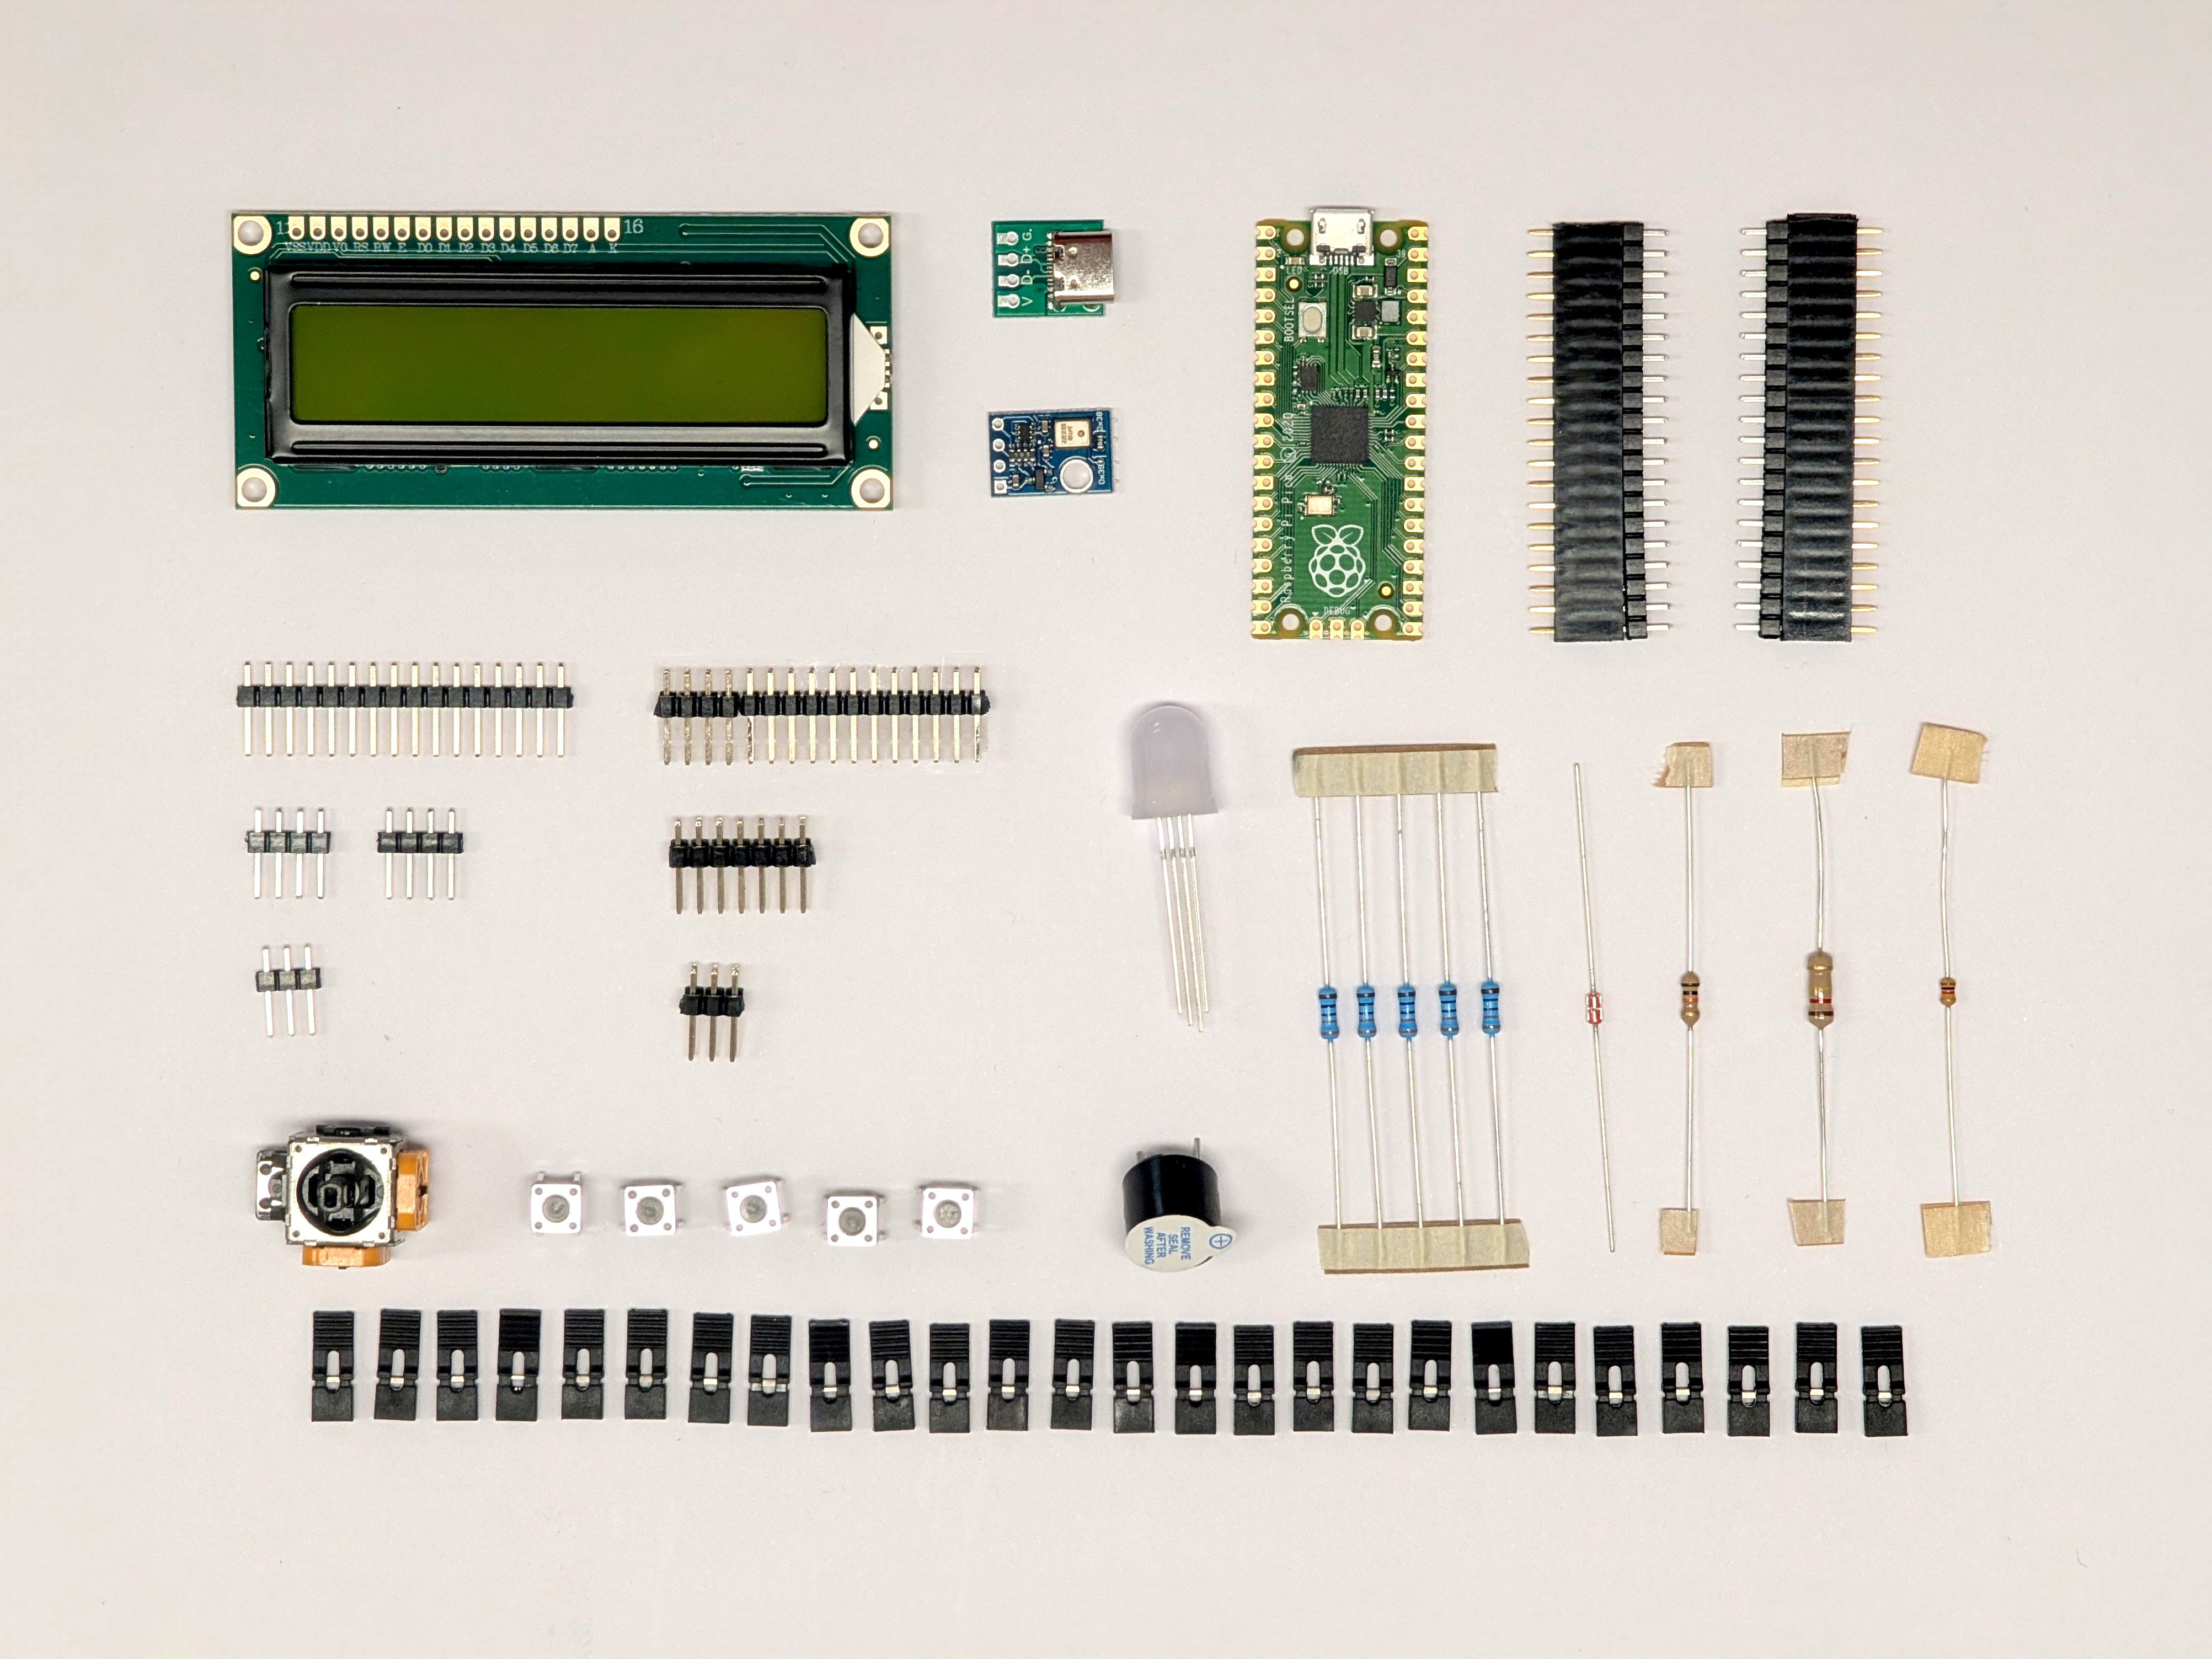
\includegraphics[width=0.8\textwidth]{overview_without_pcb.jpg}
\end{figure}

\subsection*{Bill of Materials}

Please check if you have all the necessary components listed below:

\begin{itemize}
    \item 1x Buzzerino circuit board (Buzzerino PCB)
    \item 1x Raspberry Pi Pico
    \item 1x 1602A LCD display
    \item 1x AHT10 digital temperature and humidity sensor
    \item 1x USB-C breakout board
    \item 1x 10 mm RGB LED
    \item 1x buzzer
    \item 1x analogue joystick
    \item 5x 6 mm push buttons
    \item 1x 100 k$\Omega$ NTC temperature-dependent resistor
    \item 5x 330 $\Omega$ resistors
    \item 1x 1 k$\Omega$ resistor
    \item 1x 10 k$\Omega$ resistor
    \item 1x 120 k$\Omega$ resistor
    \item 2x 1x20 pin headers and sockets (keep them plugged together)
    \item 1x 1x16 pin header
    \item 2x 1x4 pin headers
    \item 1x 1x3 pin header
    \item 1x 2x16 pin header
    \item 1x 2x7 pin header
    \item 1x 2x3 pin header
    \item 26x jumper
\end{itemize}

\subsection*{Assembly of the Raspberry Pi Pico}

\begin{figure}[H]
    \centering
    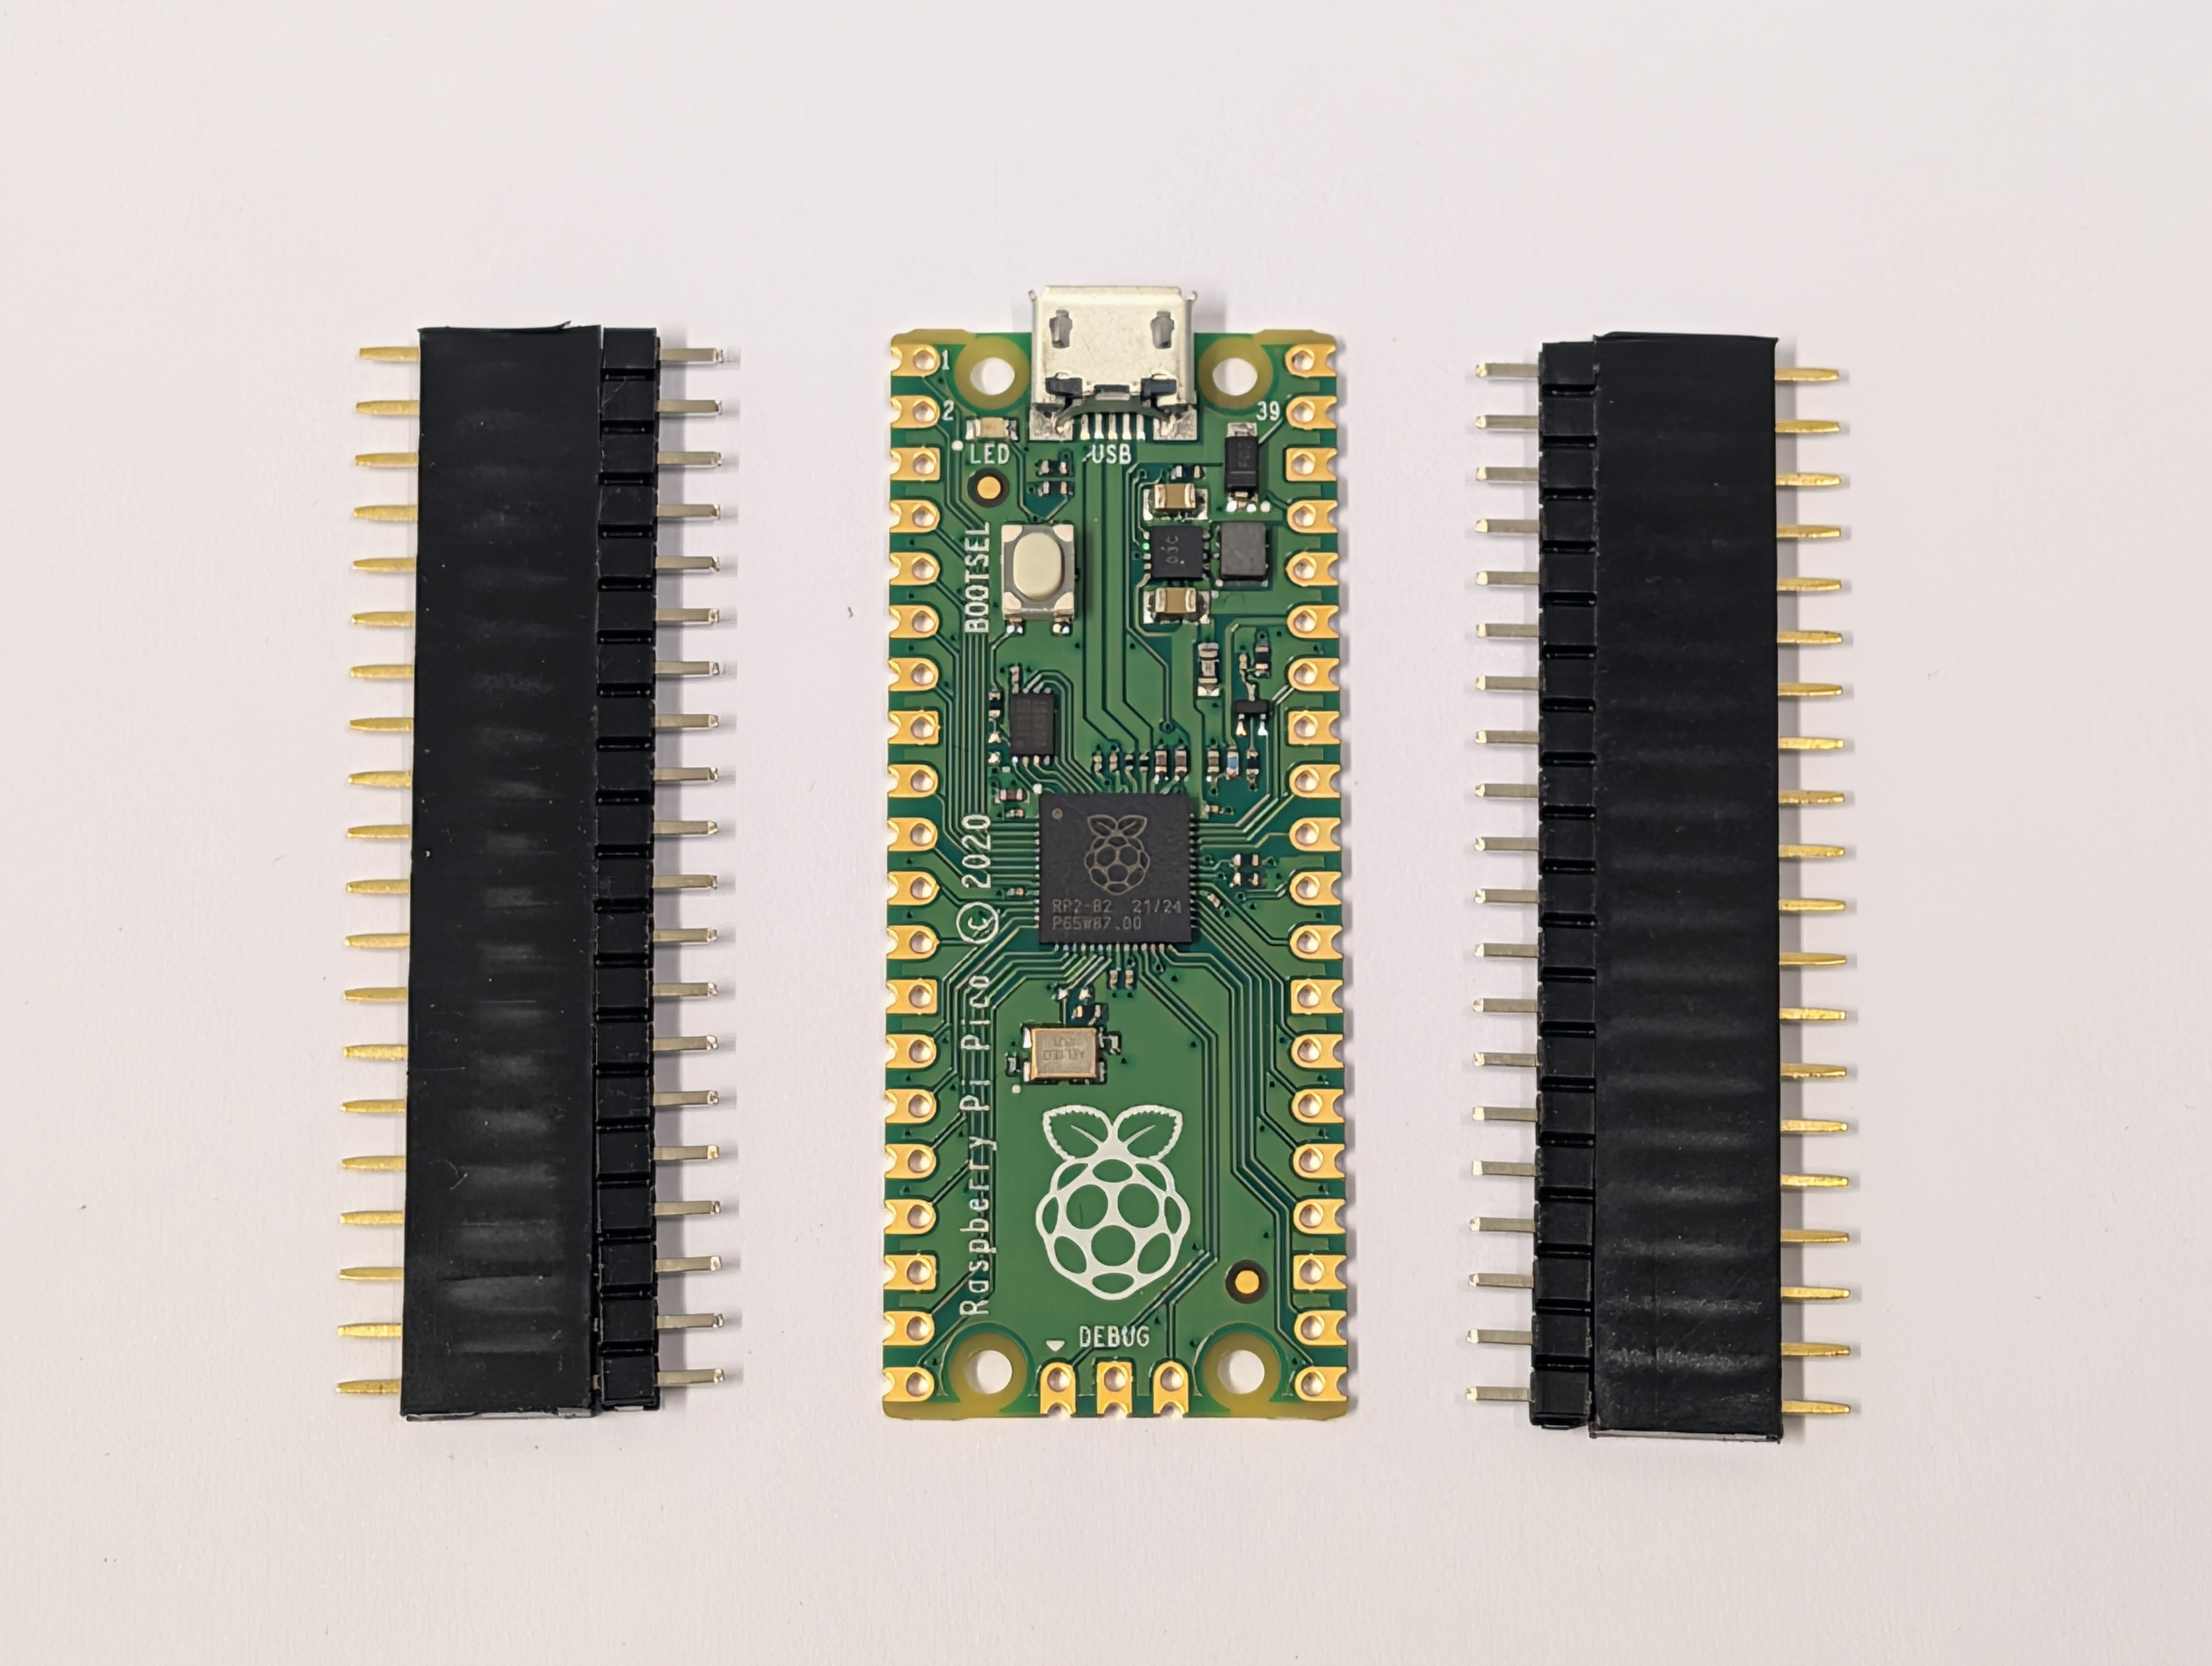
\includegraphics[width=0.75\textwidth]{pictures_of_construction/instruction_step_1.jpg}
\end{figure}

We will start by soldering the two 1x20 pin headers and sockets to the Raspberry Pi Pico board. The pin strips are each two parts plugged together; keep them together, as this will keep the contacts aligned. The side with the slimmer plastic piece will be soldered to the Raspberry Pi Pico (in the picture above, the inner one).

Start by putting the pin headers into the Raspberry Pi Pico and the Buzzerino PCB. The Raspberry Pi Pico should sit flat and parallel on both pin strips.

\begin{figure}[H]
    \centering
    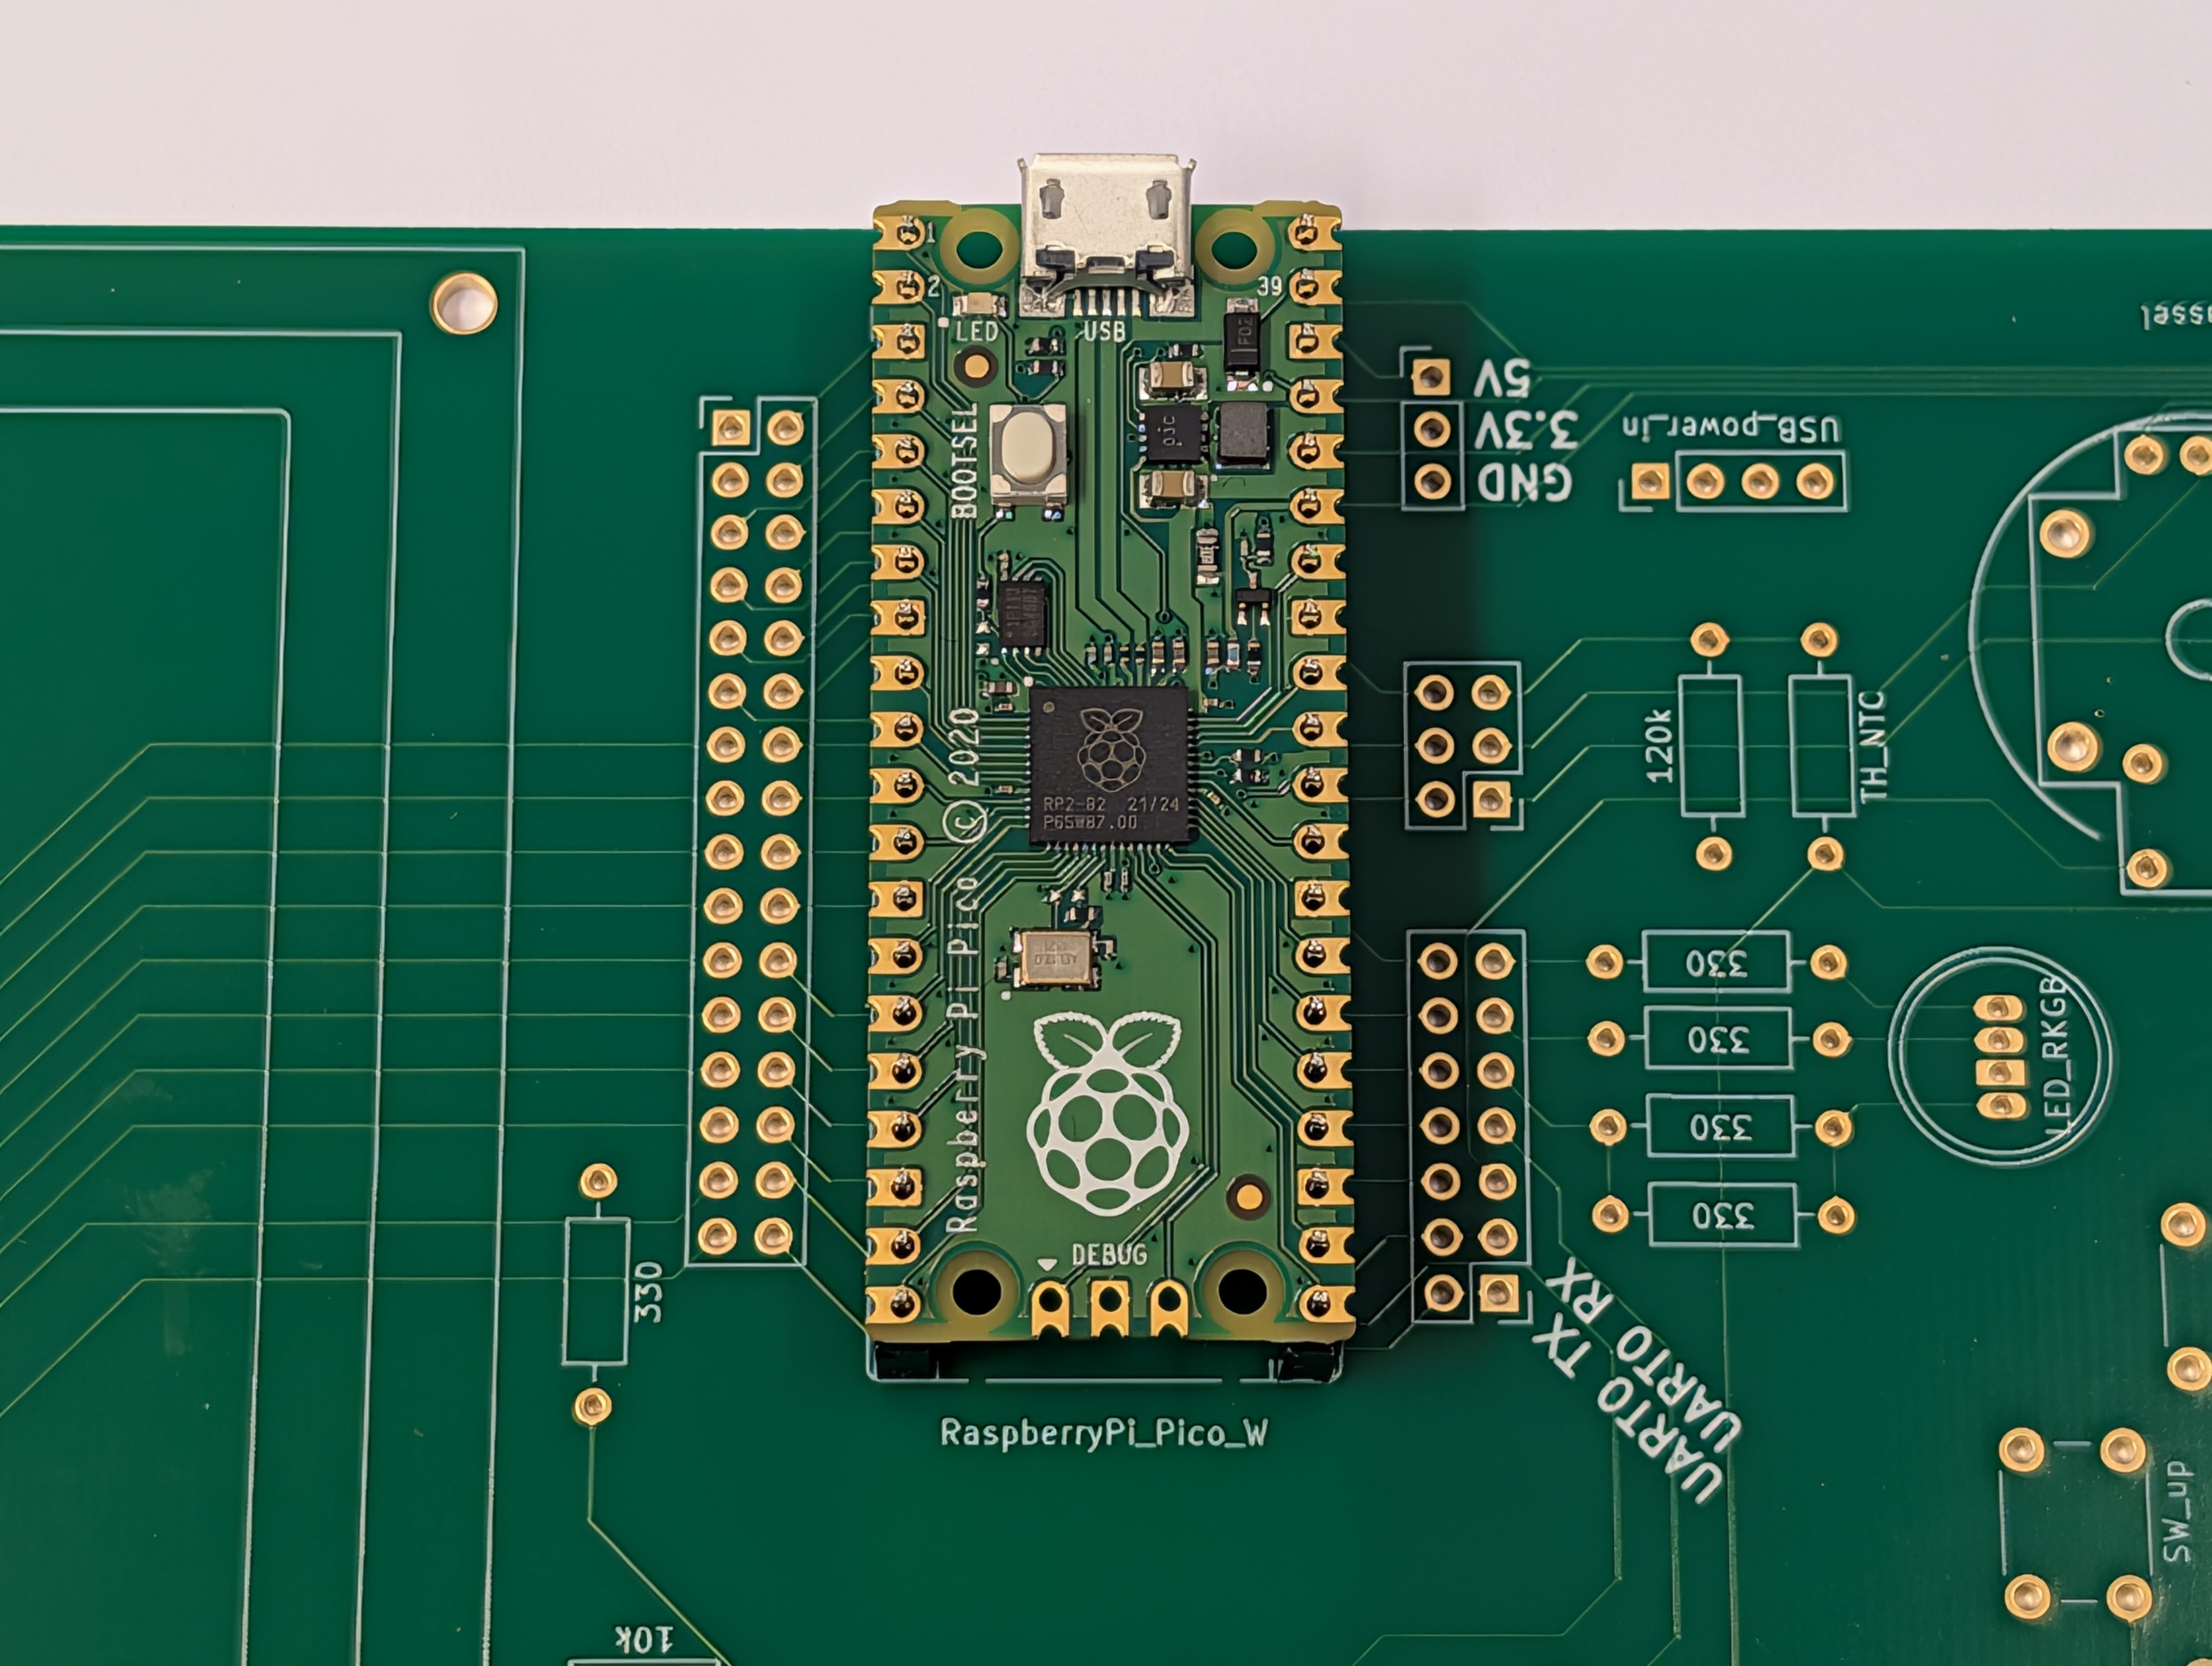
\includegraphics[width=0.75\textwidth]{pictures_of_construction/instruction_step_2.jpg}
\end{figure}

Now we can solder our first connections. Heat one of the corner pins with your soldering iron. Check with solder whether the joint is up to temperature by gently feeding it into the heated pin. If the solder melts, you can remove the soldering iron and let the connection cool down.

\begin{figure}[H]
    \centering
    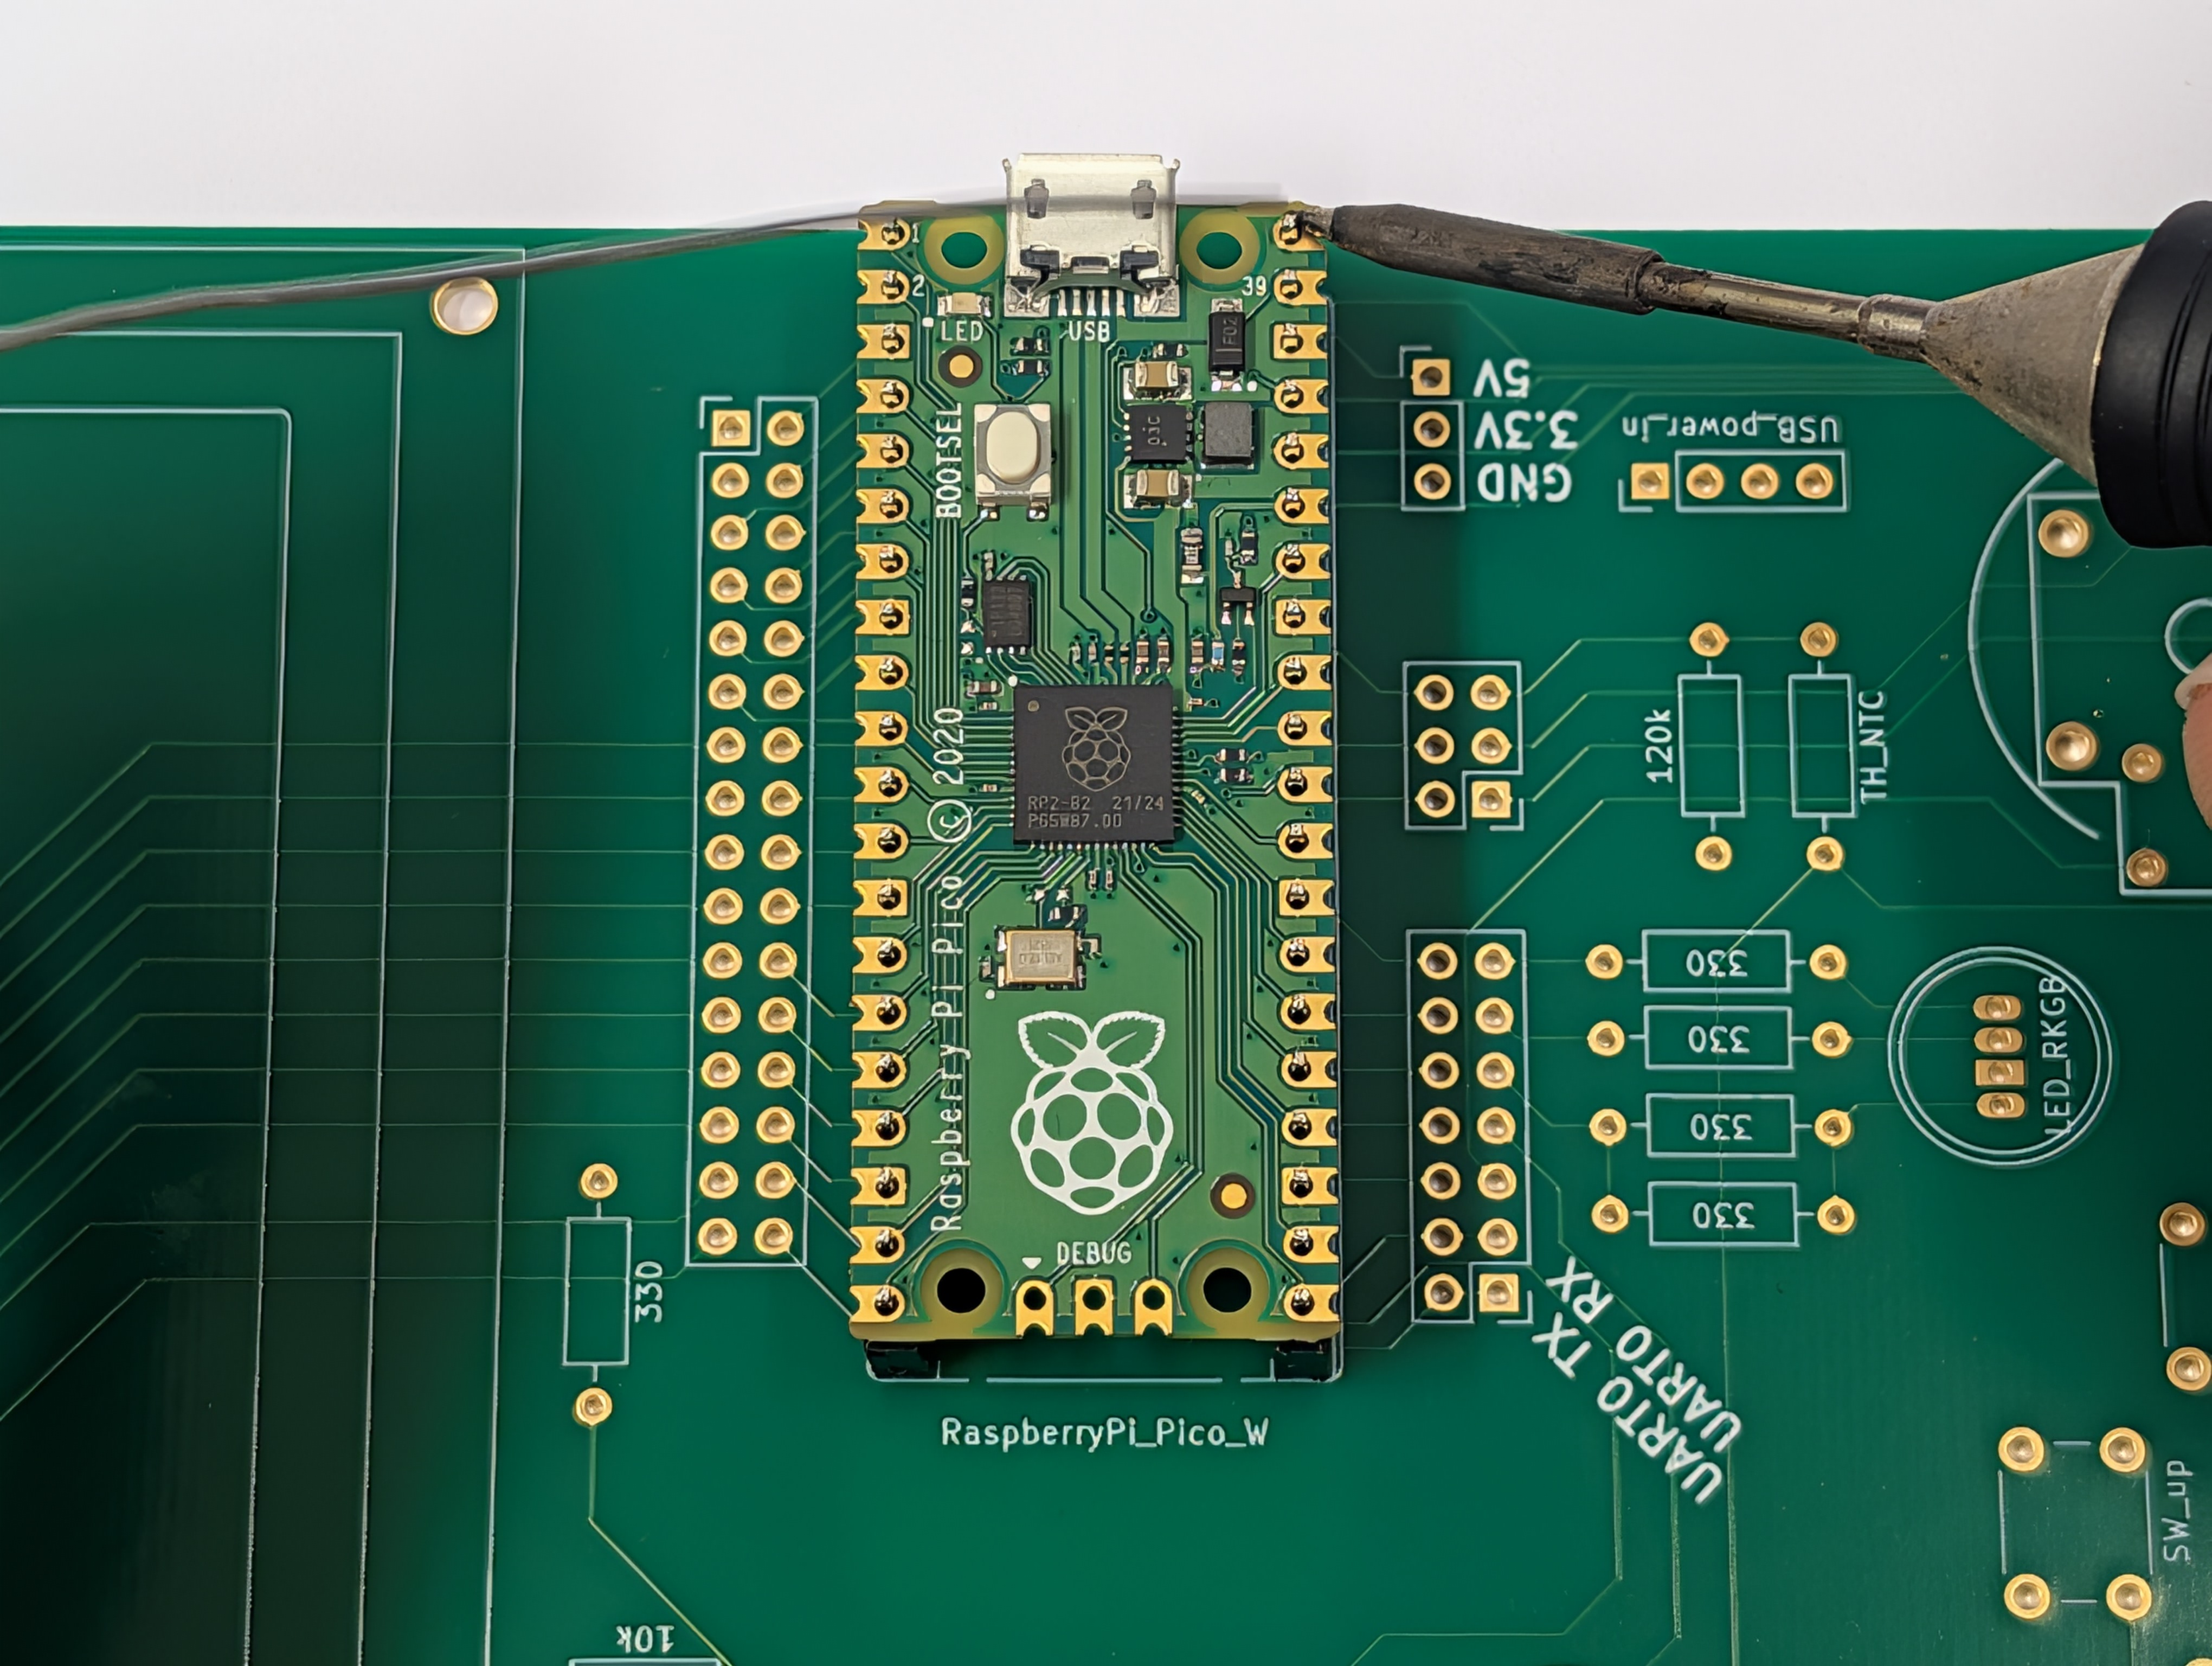
\includegraphics[width=0.75\textwidth]{pictures_of_construction/instruction_step_3.jpg}
\end{figure}

Continue by soldering the three other corners.

\begin{figure}[H]
    \centering
    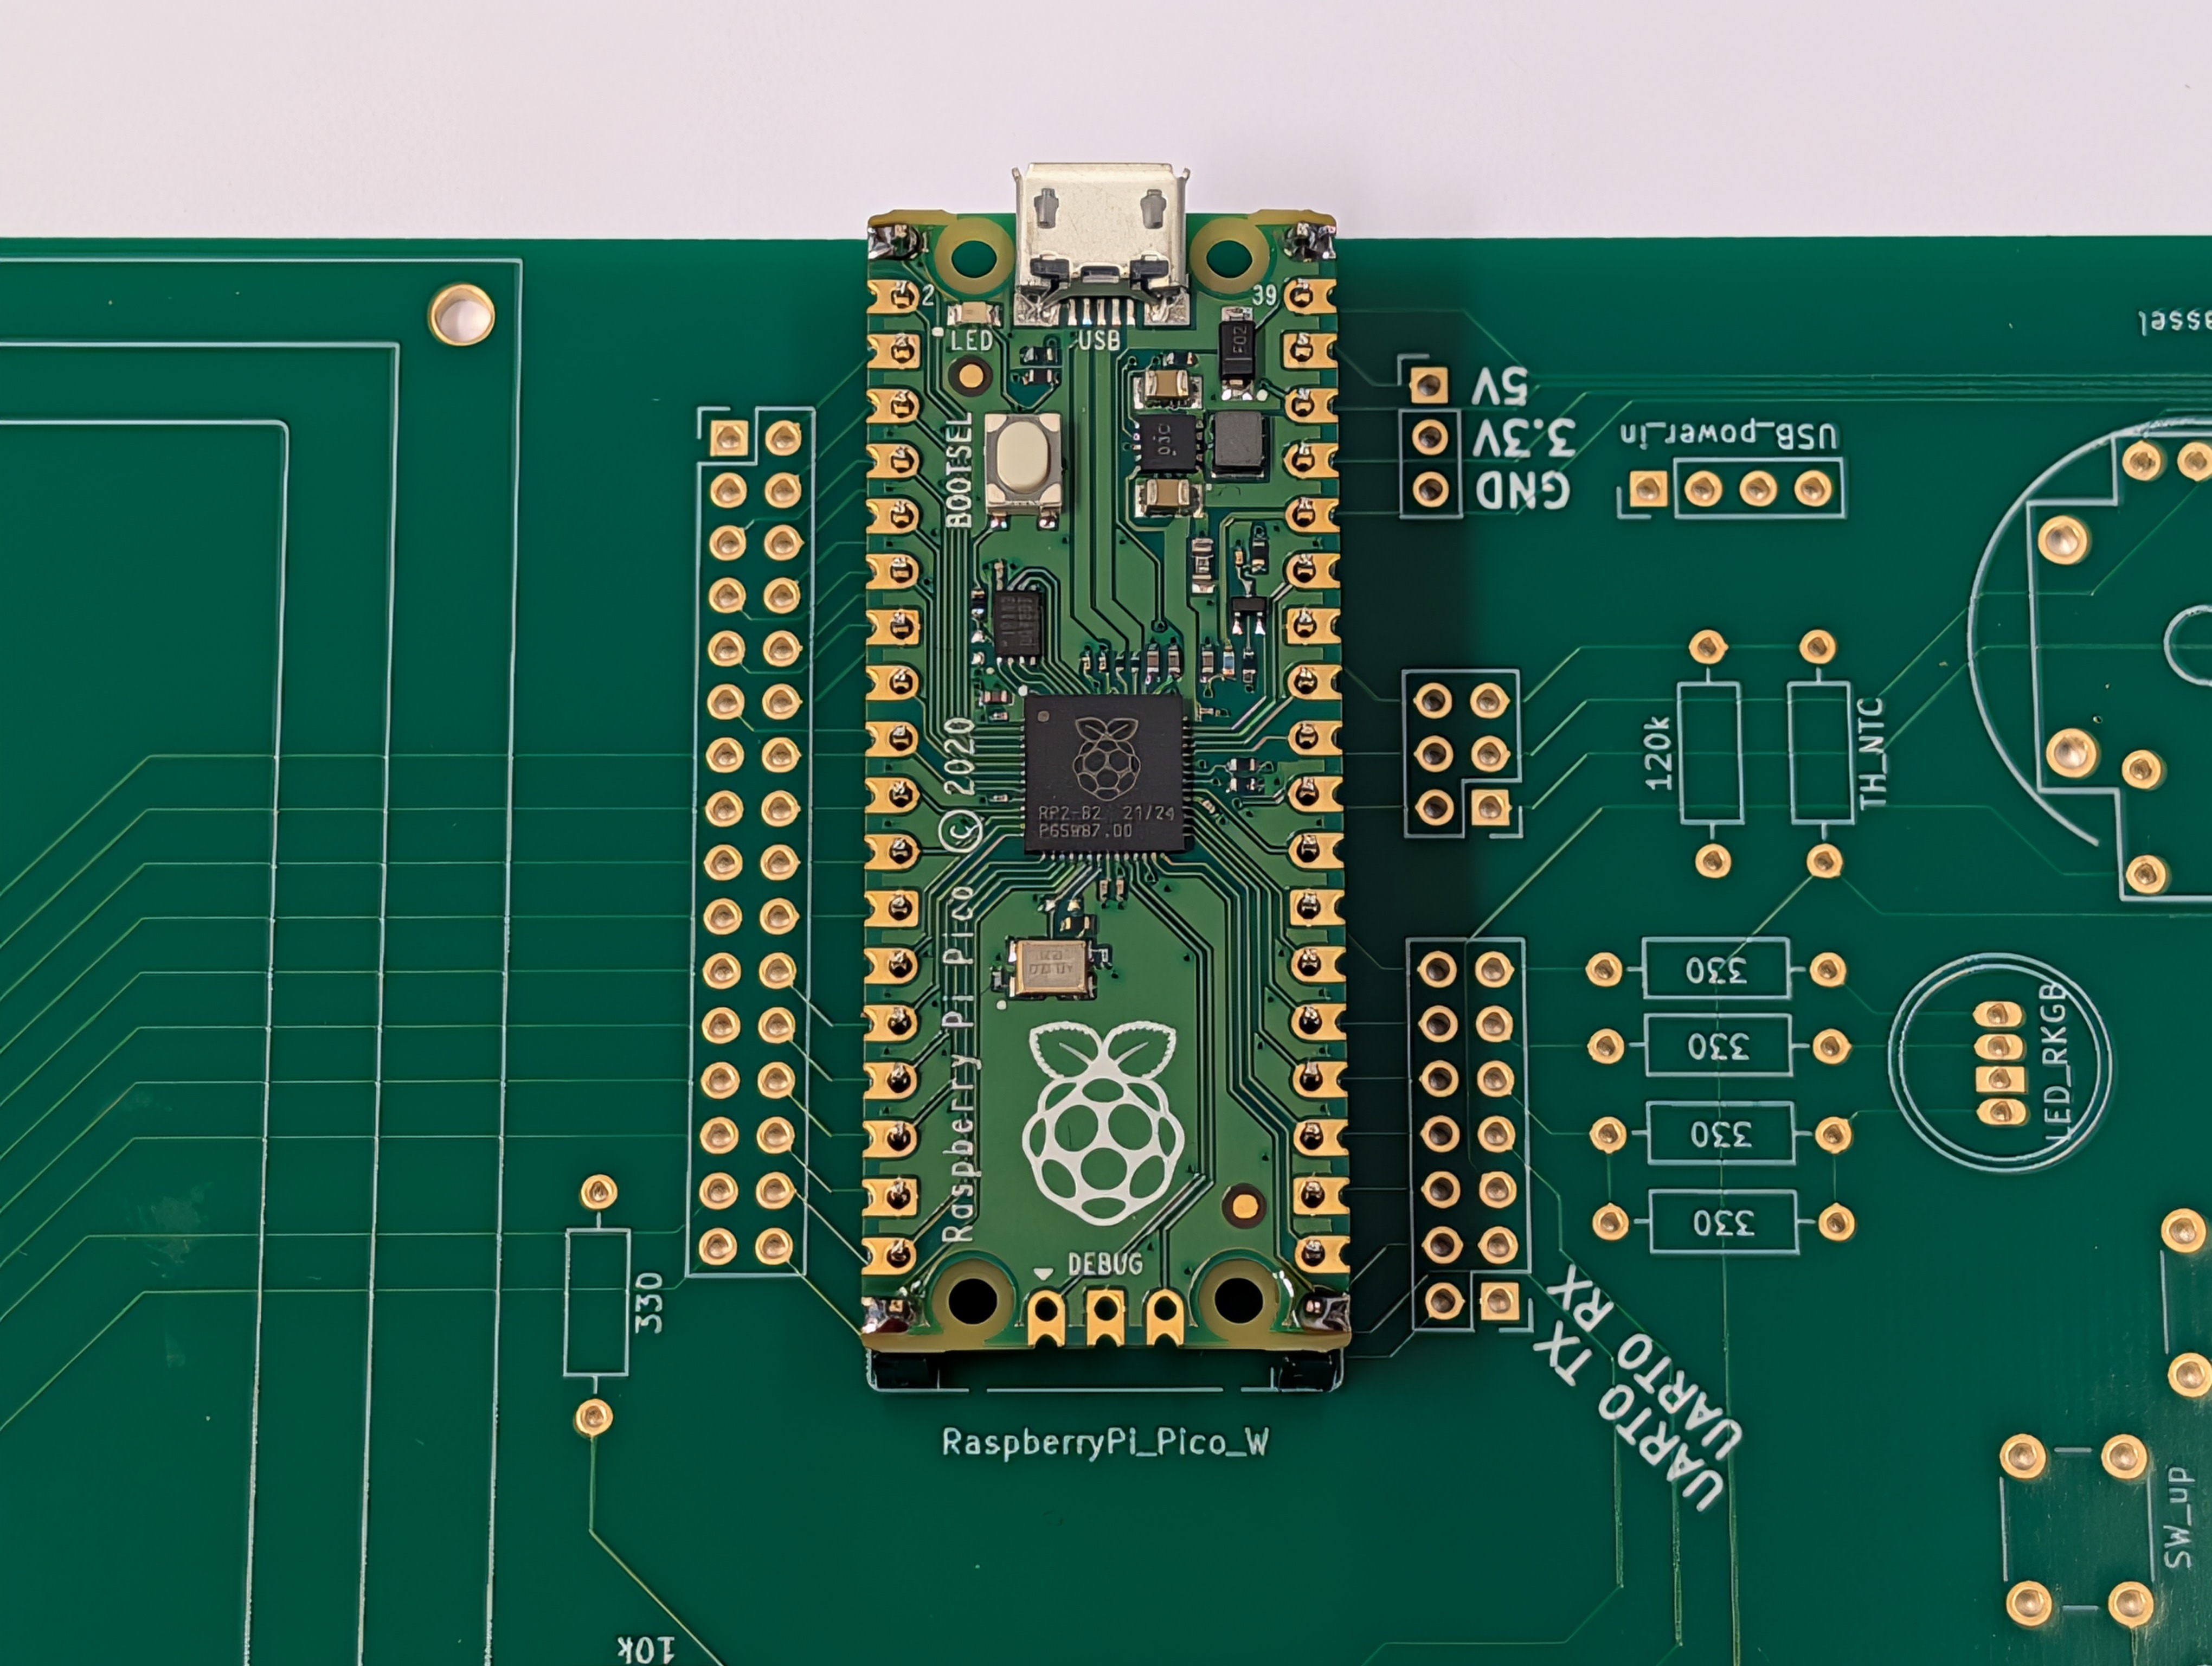
\includegraphics[width=0.75\textwidth]{pictures_of_construction/instruction_step_4.jpg}
\end{figure}

Now you can remove the Raspberry Pi Pico from the Buzzerino PCB (with the pin headers still together).

\begin{figure}[H]
    \centering
    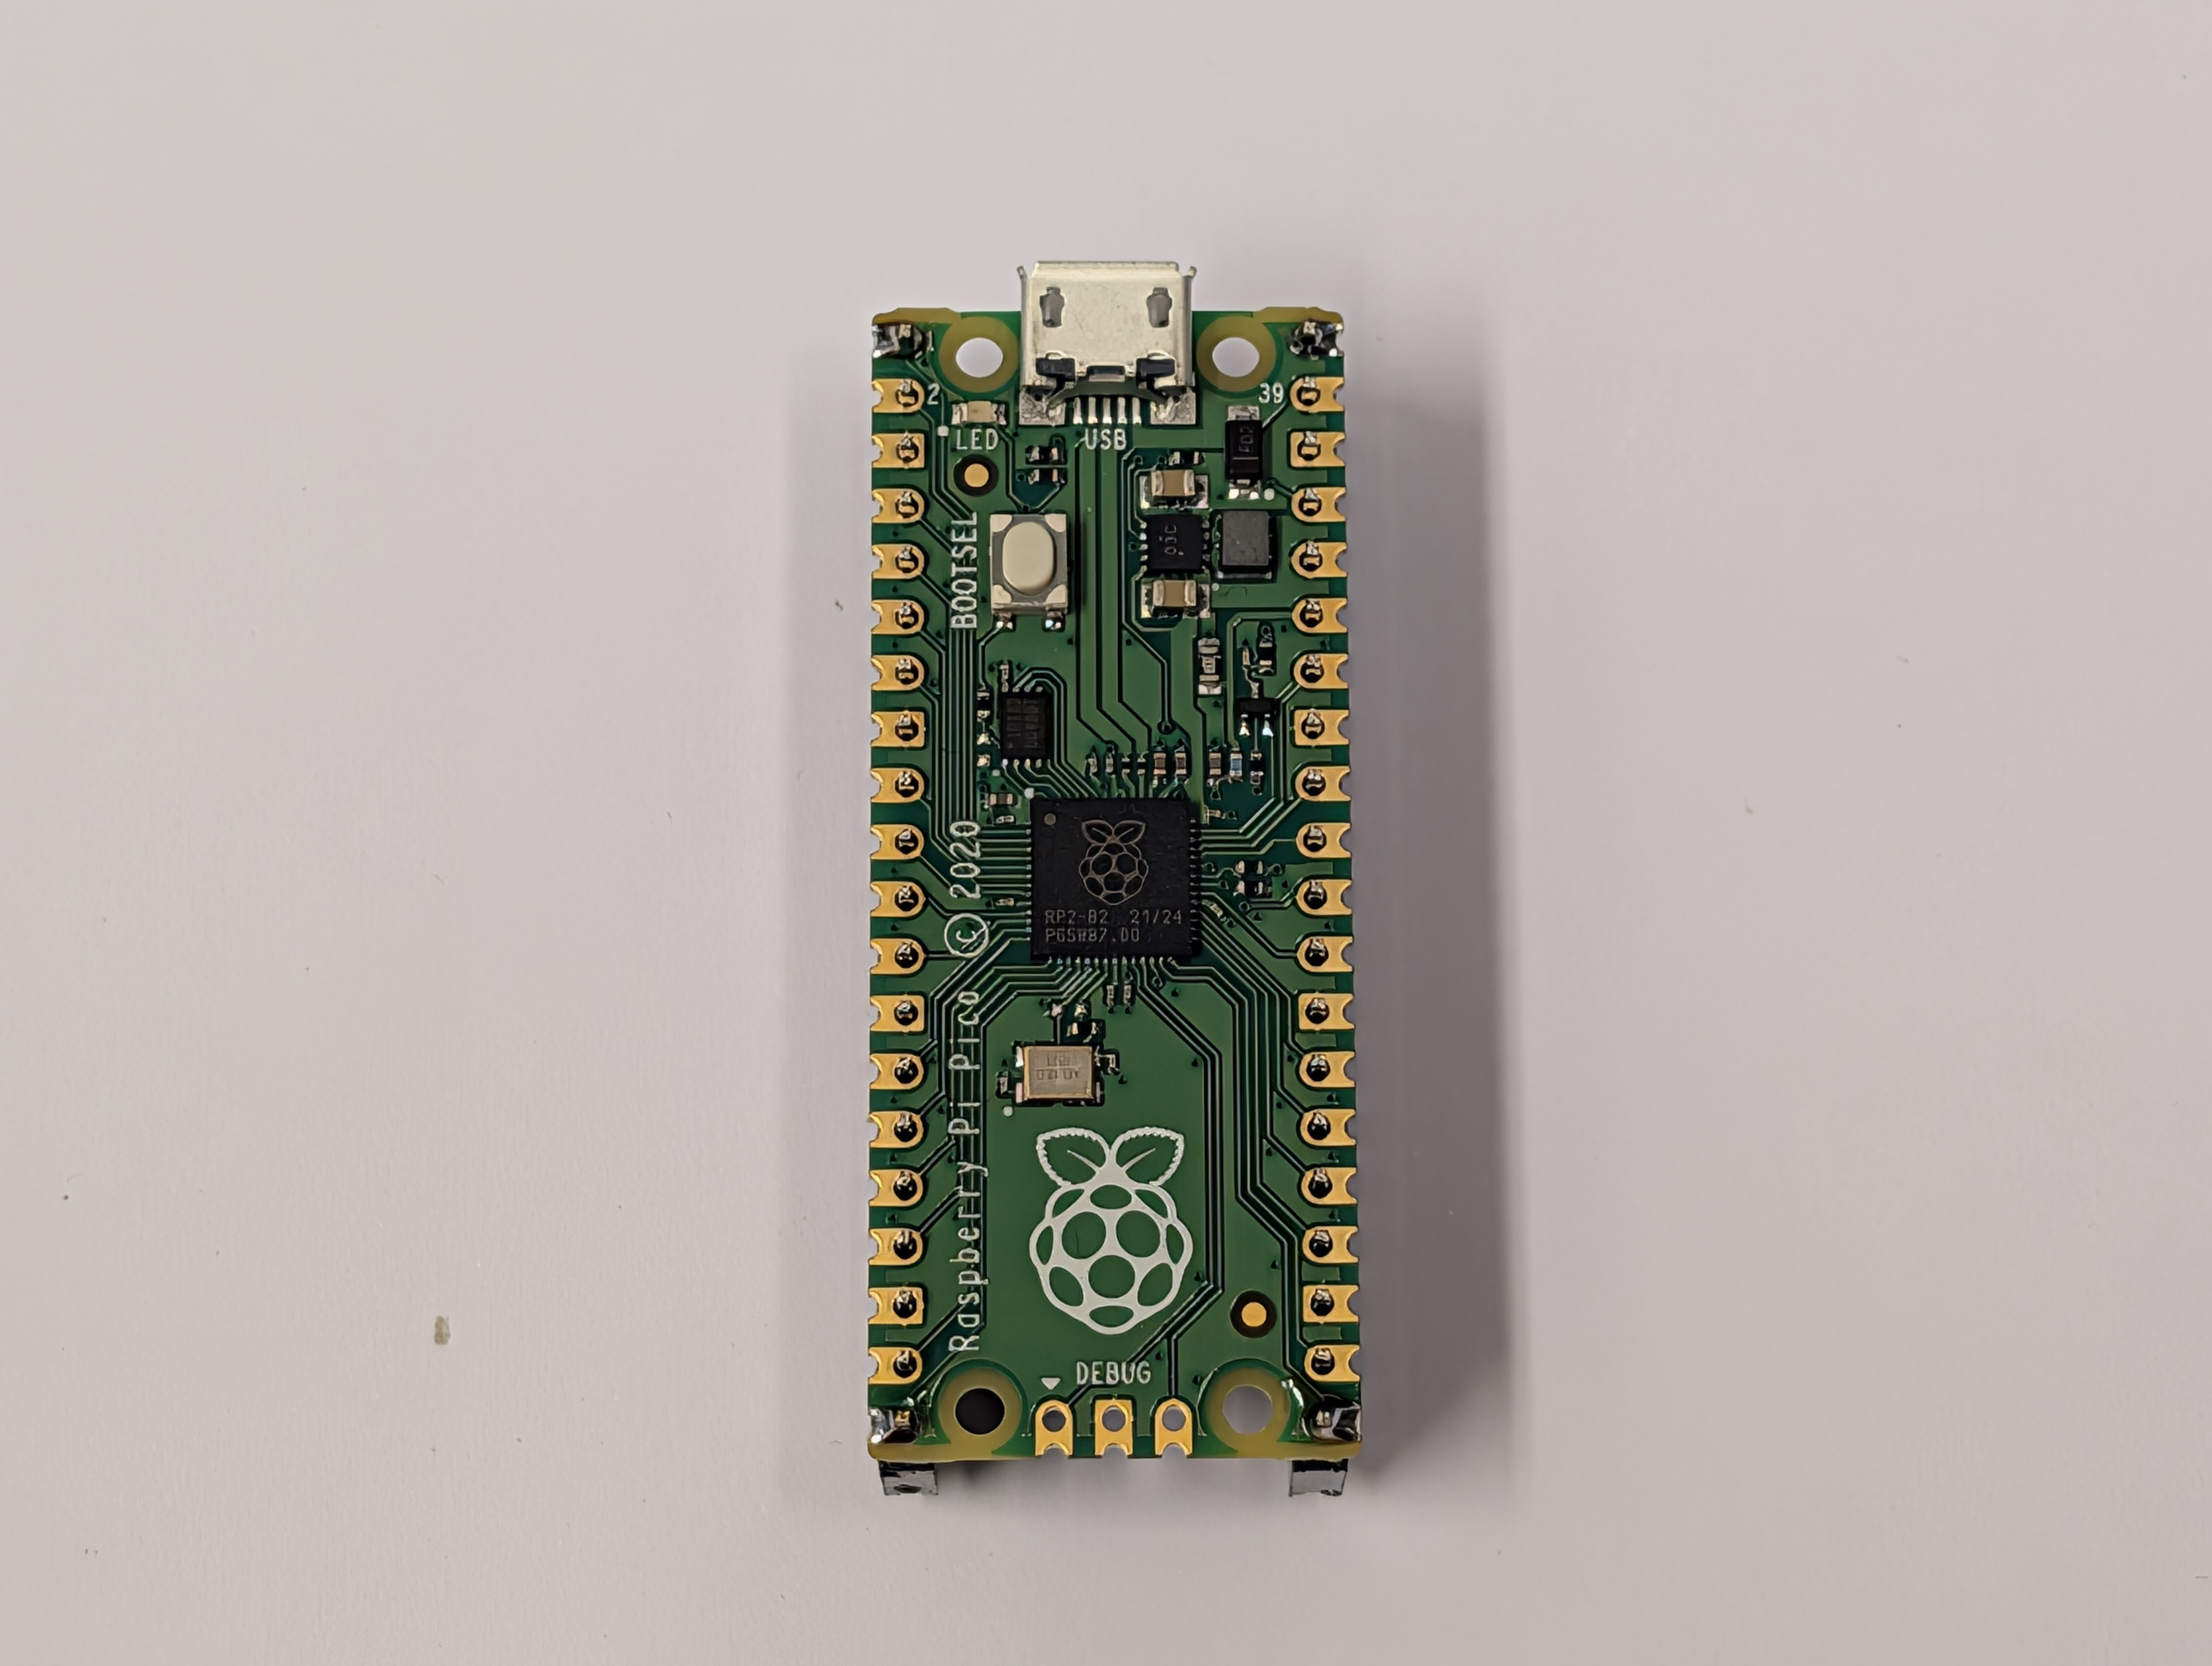
\includegraphics[width=0.75\textwidth]{pictures_of_construction/instruction_step_5.jpg}
\end{figure}

With the Raspberry Pi Pico now free, but the pin strips still attached to it, you can fully solder both sides.

\begin{figure}[H]
    \centering
    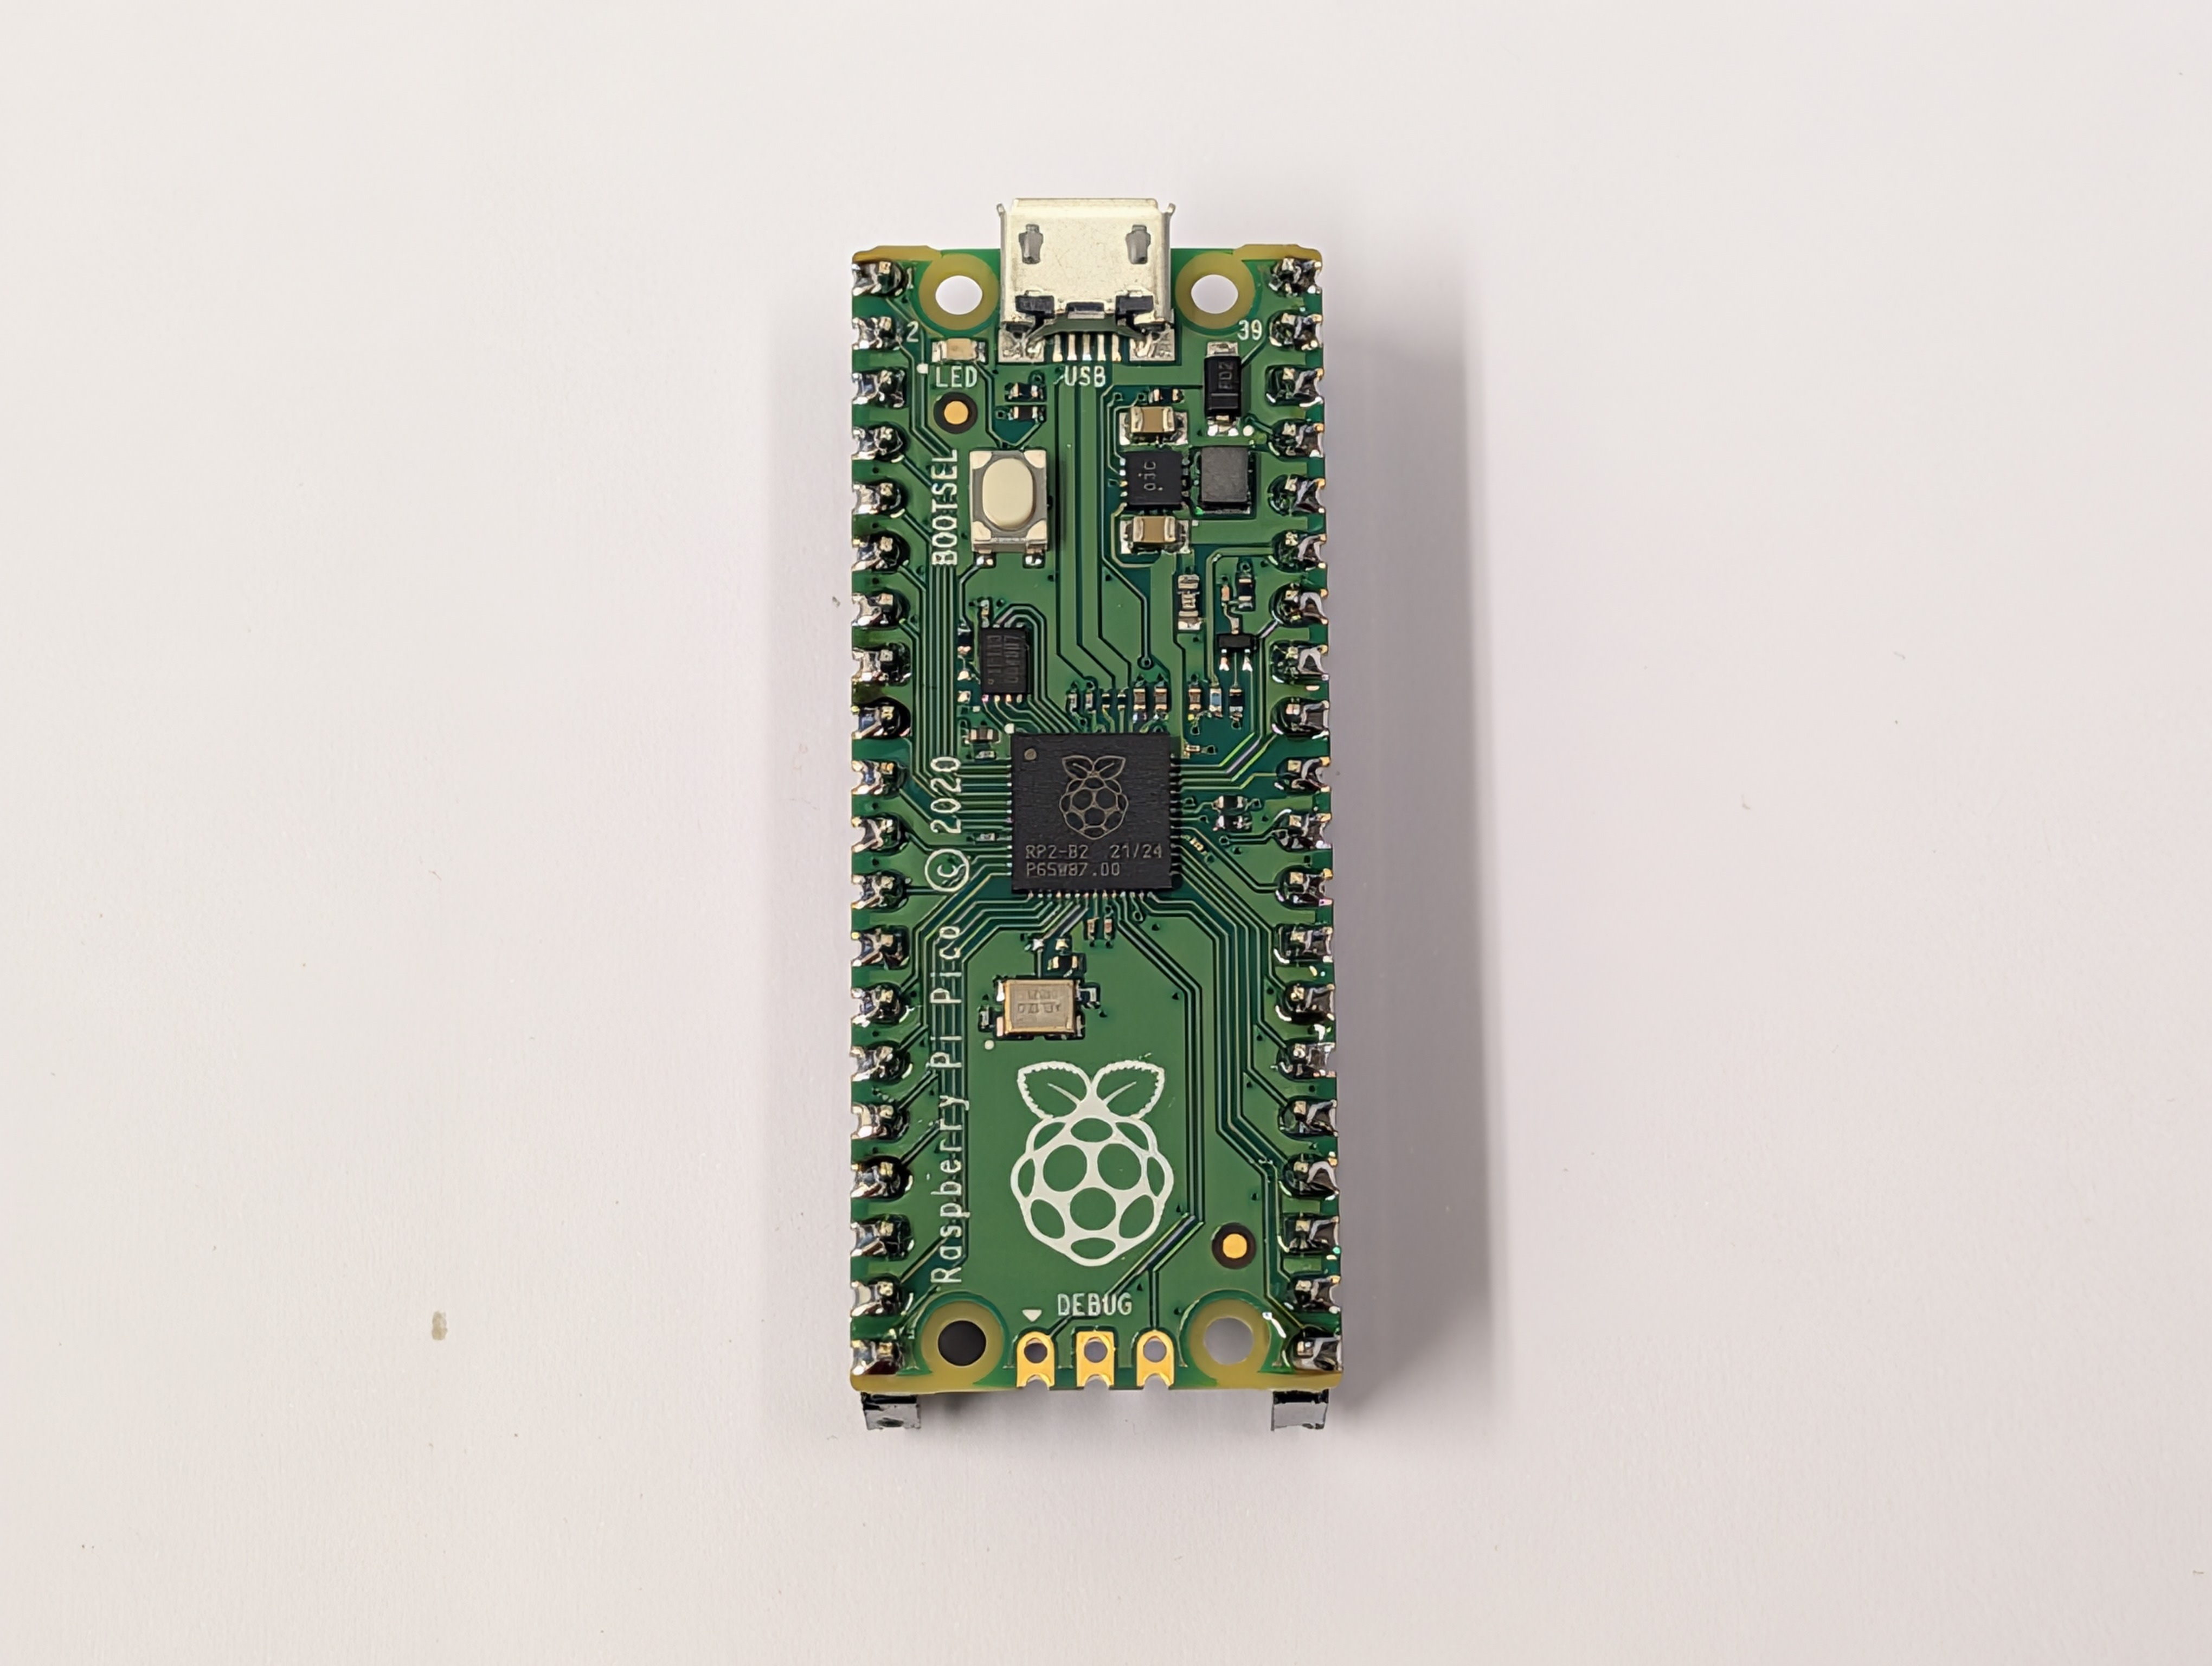
\includegraphics[width=0.75\textwidth]{pictures_of_construction/instruction_step_6.jpg}
\end{figure}

\subsection*{Assembly of the USB-C breakout board}

\begin{figure}[H]
    \centering
    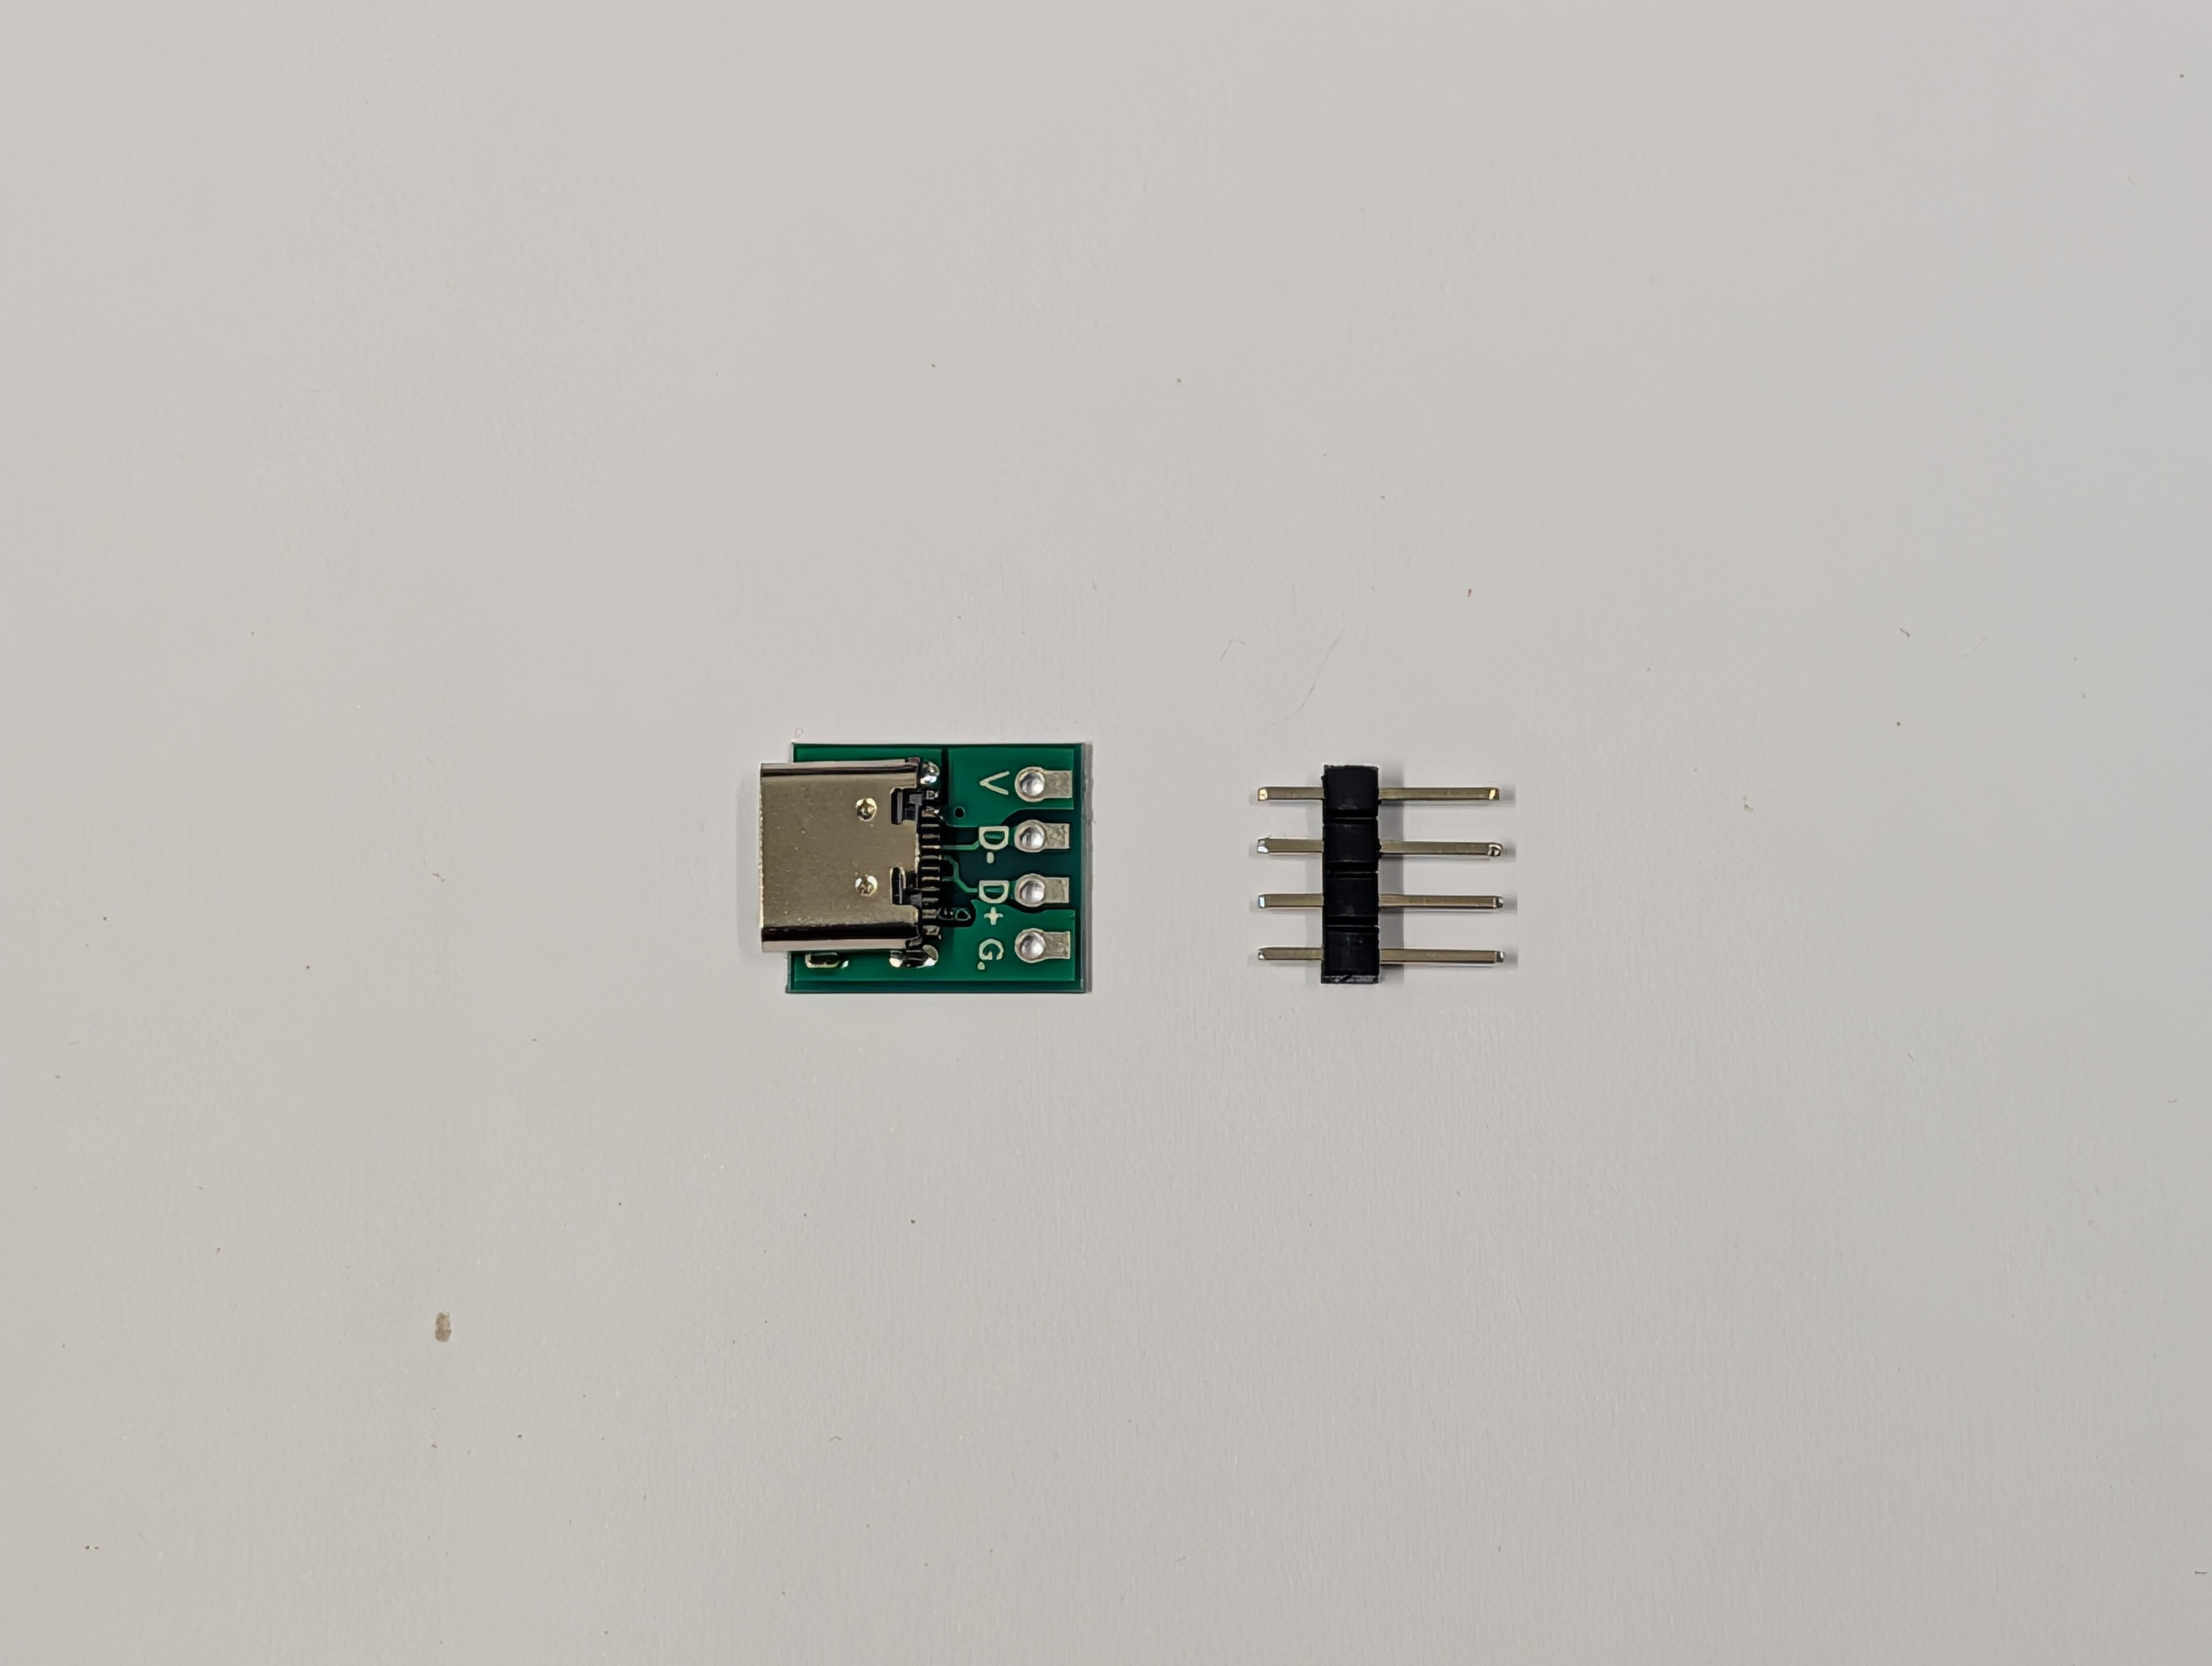
\includegraphics[width=0.75\textwidth]{pictures_of_construction/instruction_step_7.jpg}
\end{figure}

Now we will solder the 1x4 pin header to the USB-C breakout board. Because both pieces are very small, it is a good tactic to plug them together and place them on your table.

\begin{figure}[H]
    \centering
    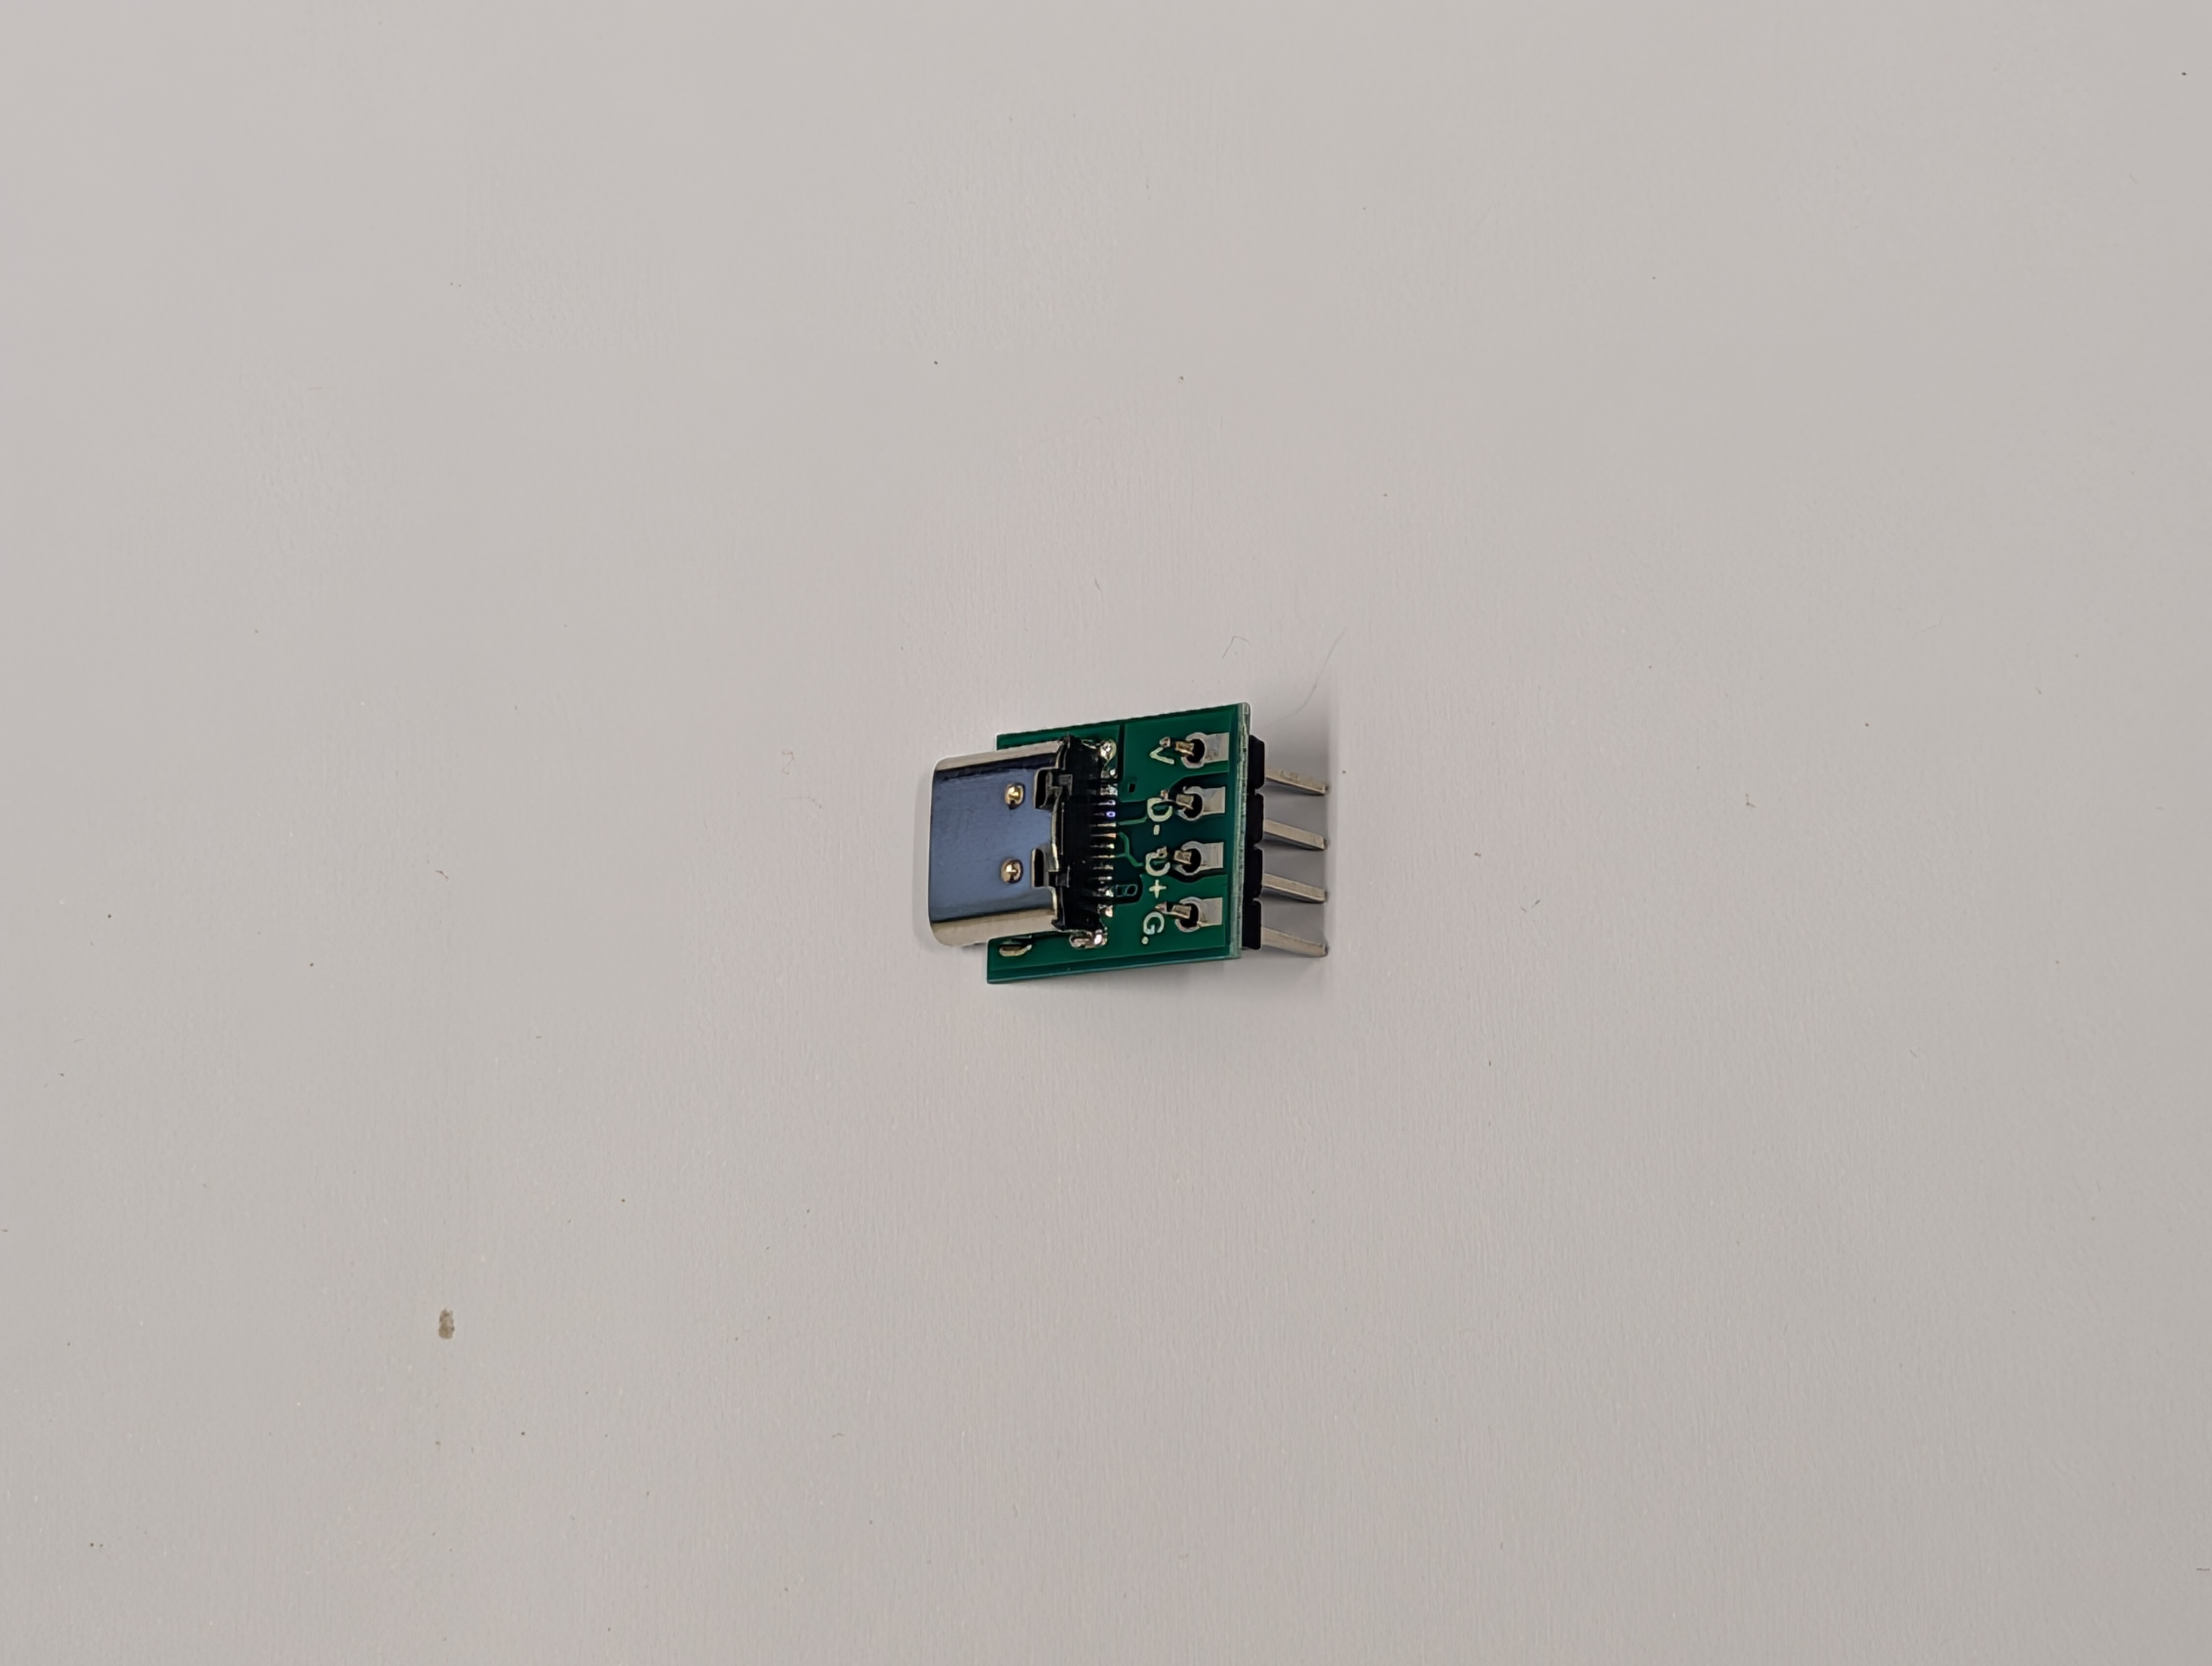
\includegraphics[width=0.75\textwidth]{pictures_of_construction/instruction_step_8.jpg}
\end{figure}

Start by soldering only one pin, as the angle between the board and the pin header will likely be slightly crooked.

\begin{figure}[H]
    \centering
    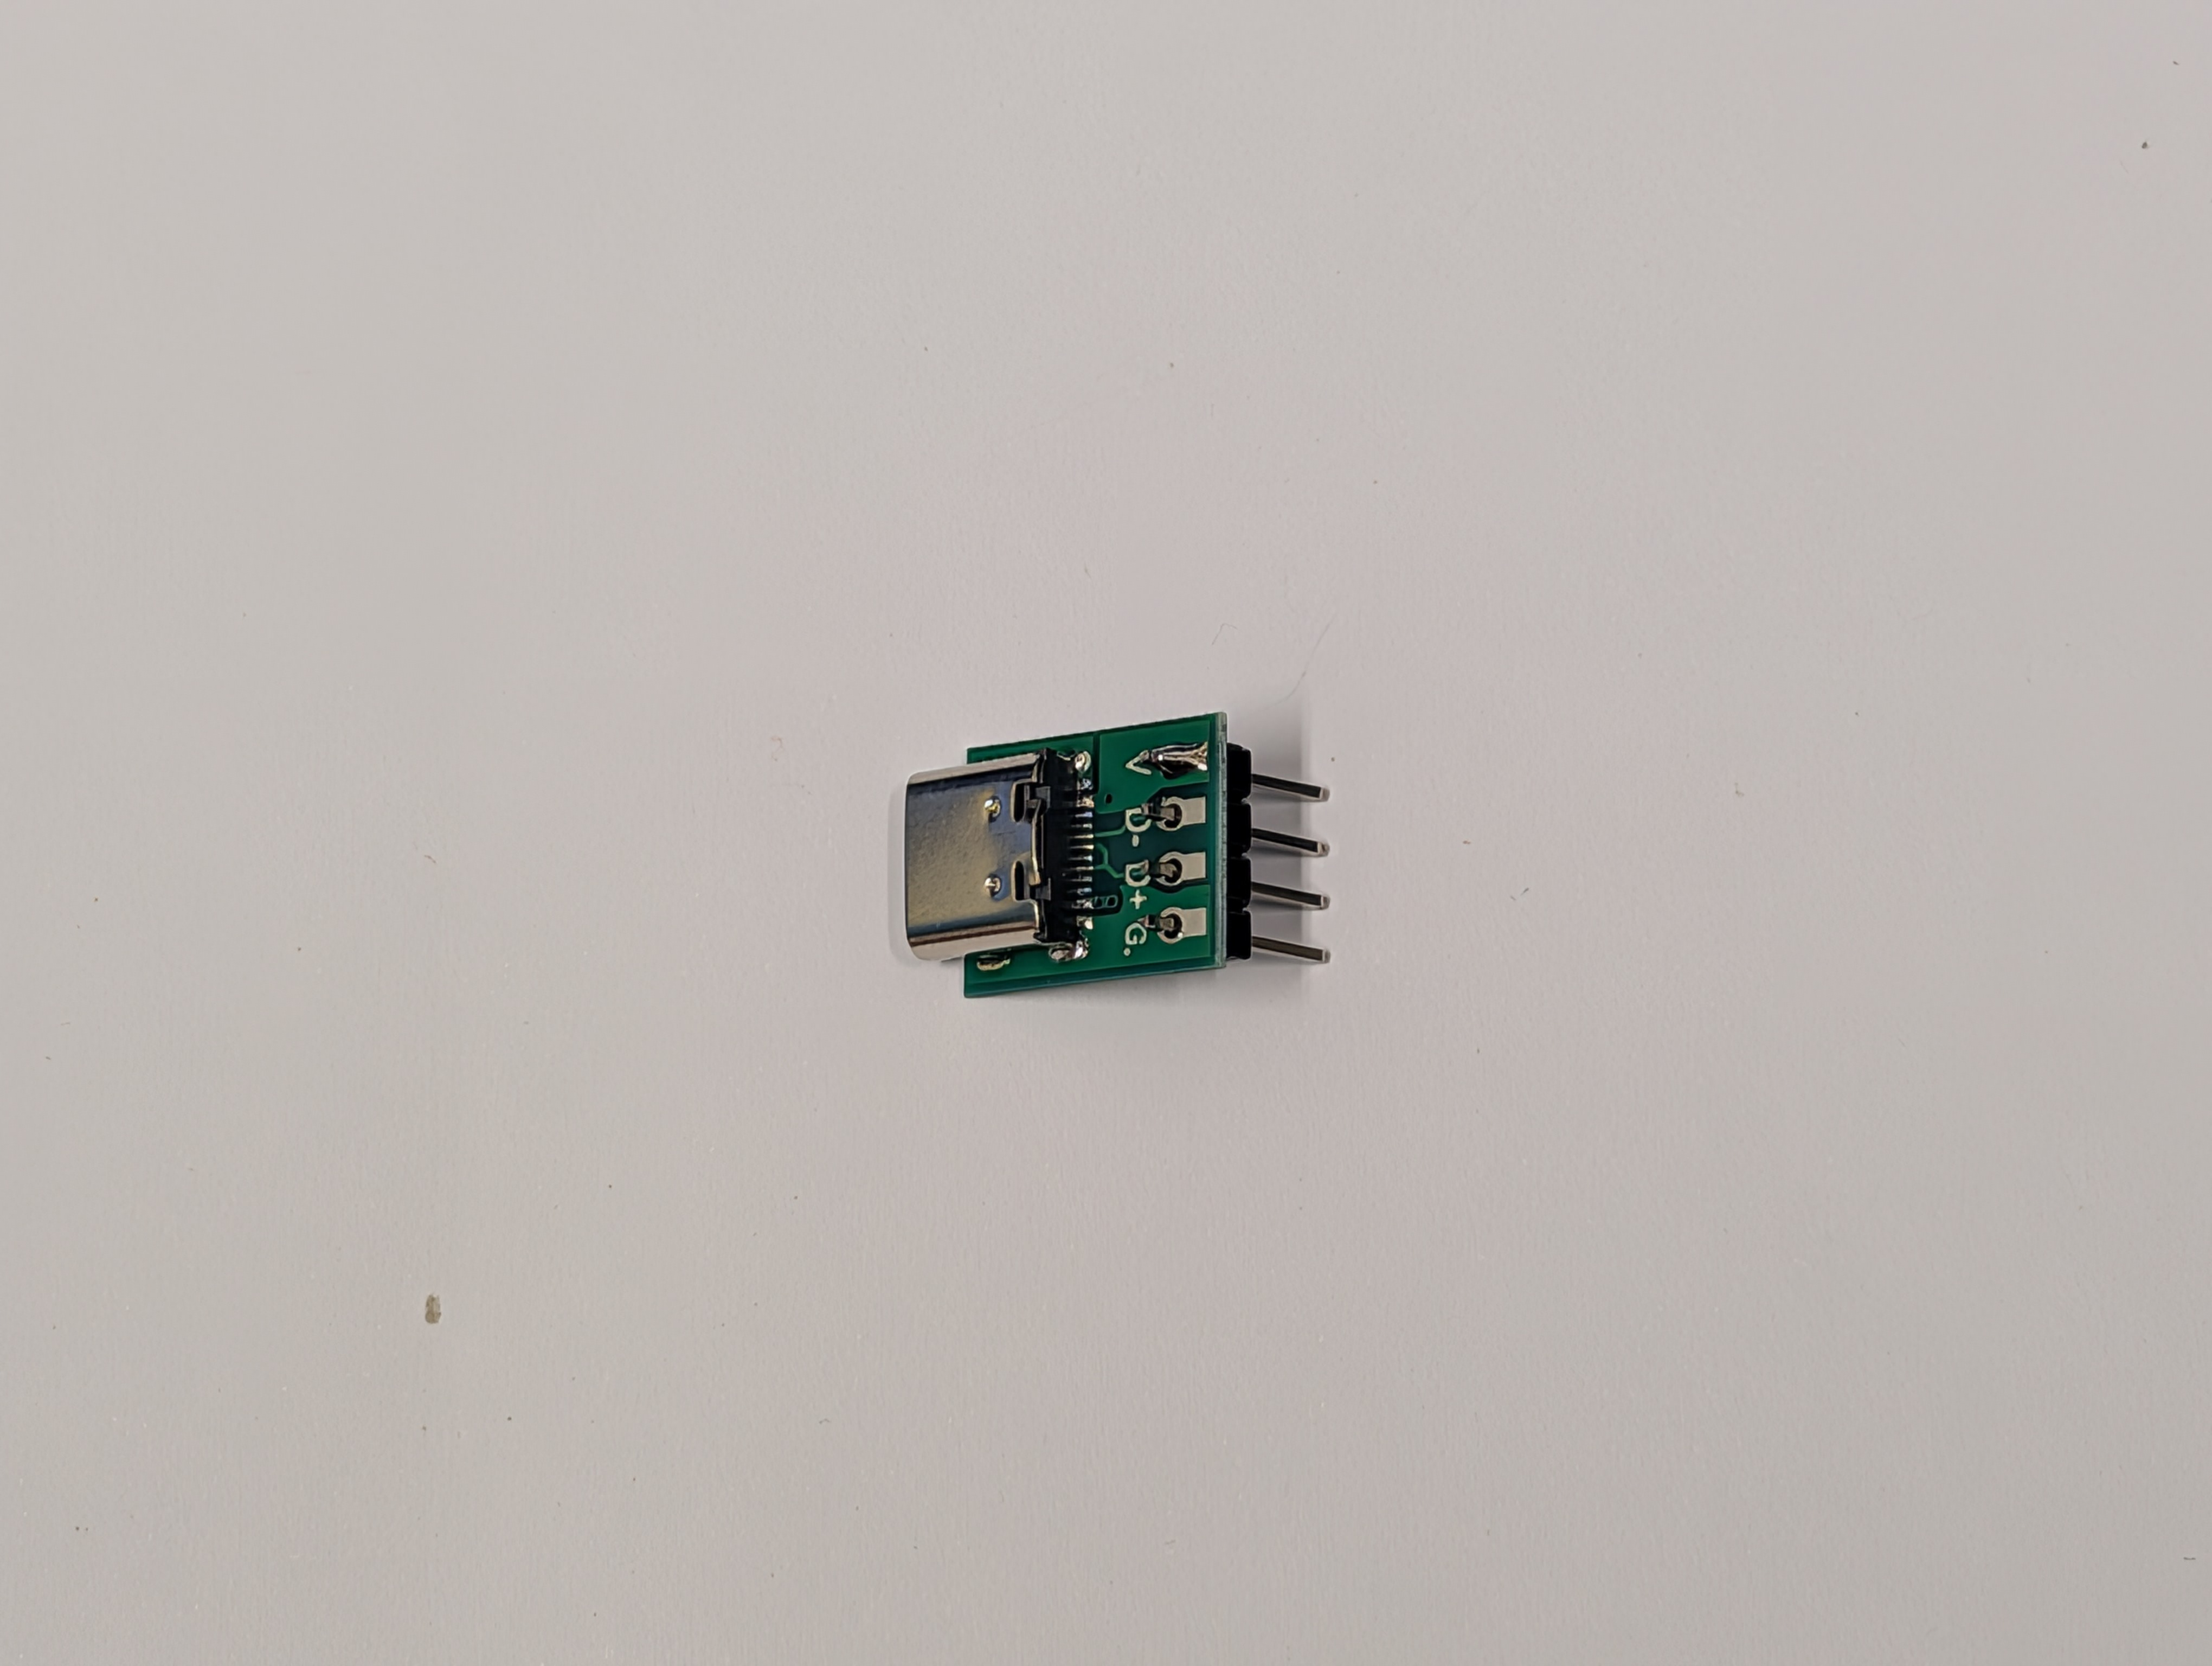
\includegraphics[width=0.75\textwidth]{pictures_of_construction/instruction_step_9.jpg}
\end{figure}

\begin{figure}[H]
    \centering
    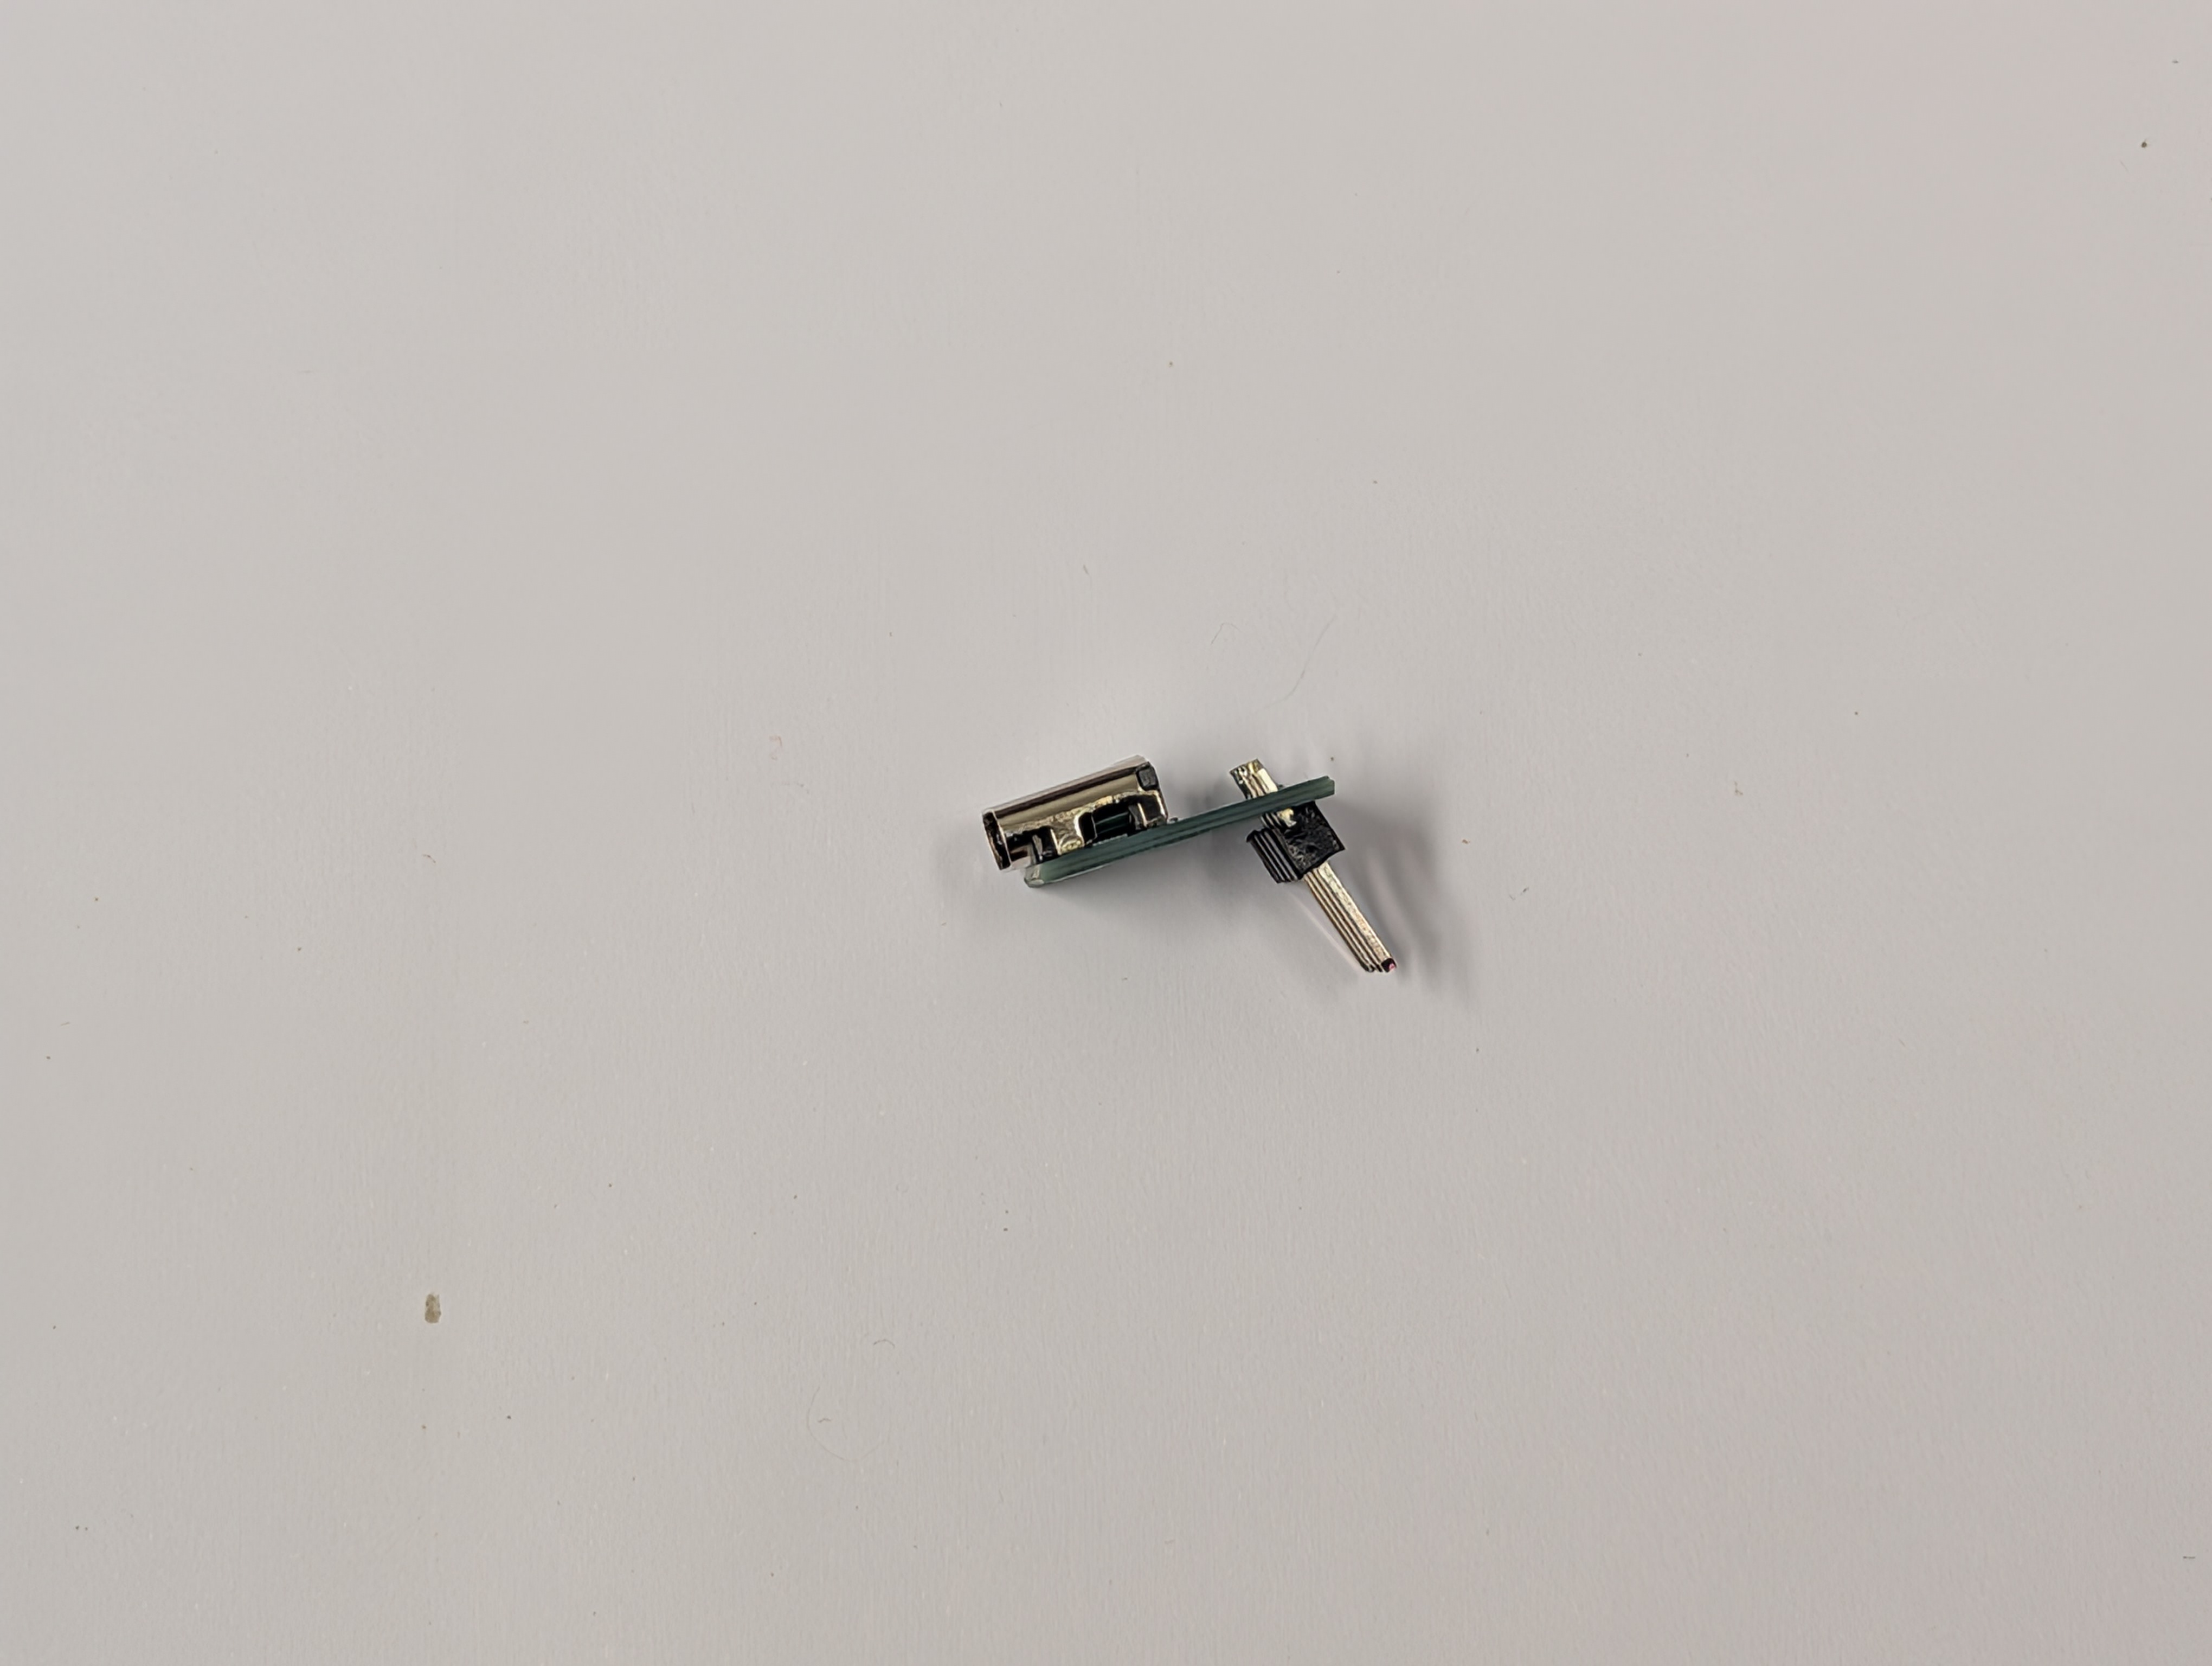
\includegraphics[width=0.75\textwidth]{pictures_of_construction/instruction_step_10.jpg}
\end{figure}

To correct the angle of the pin header, hold both pieces together and carefully reheat the solder joint. Now you can correct any misalignment. Once the pins are perpendicular to the board, solder all four pins.

\begin{figure}[H]
    \centering
    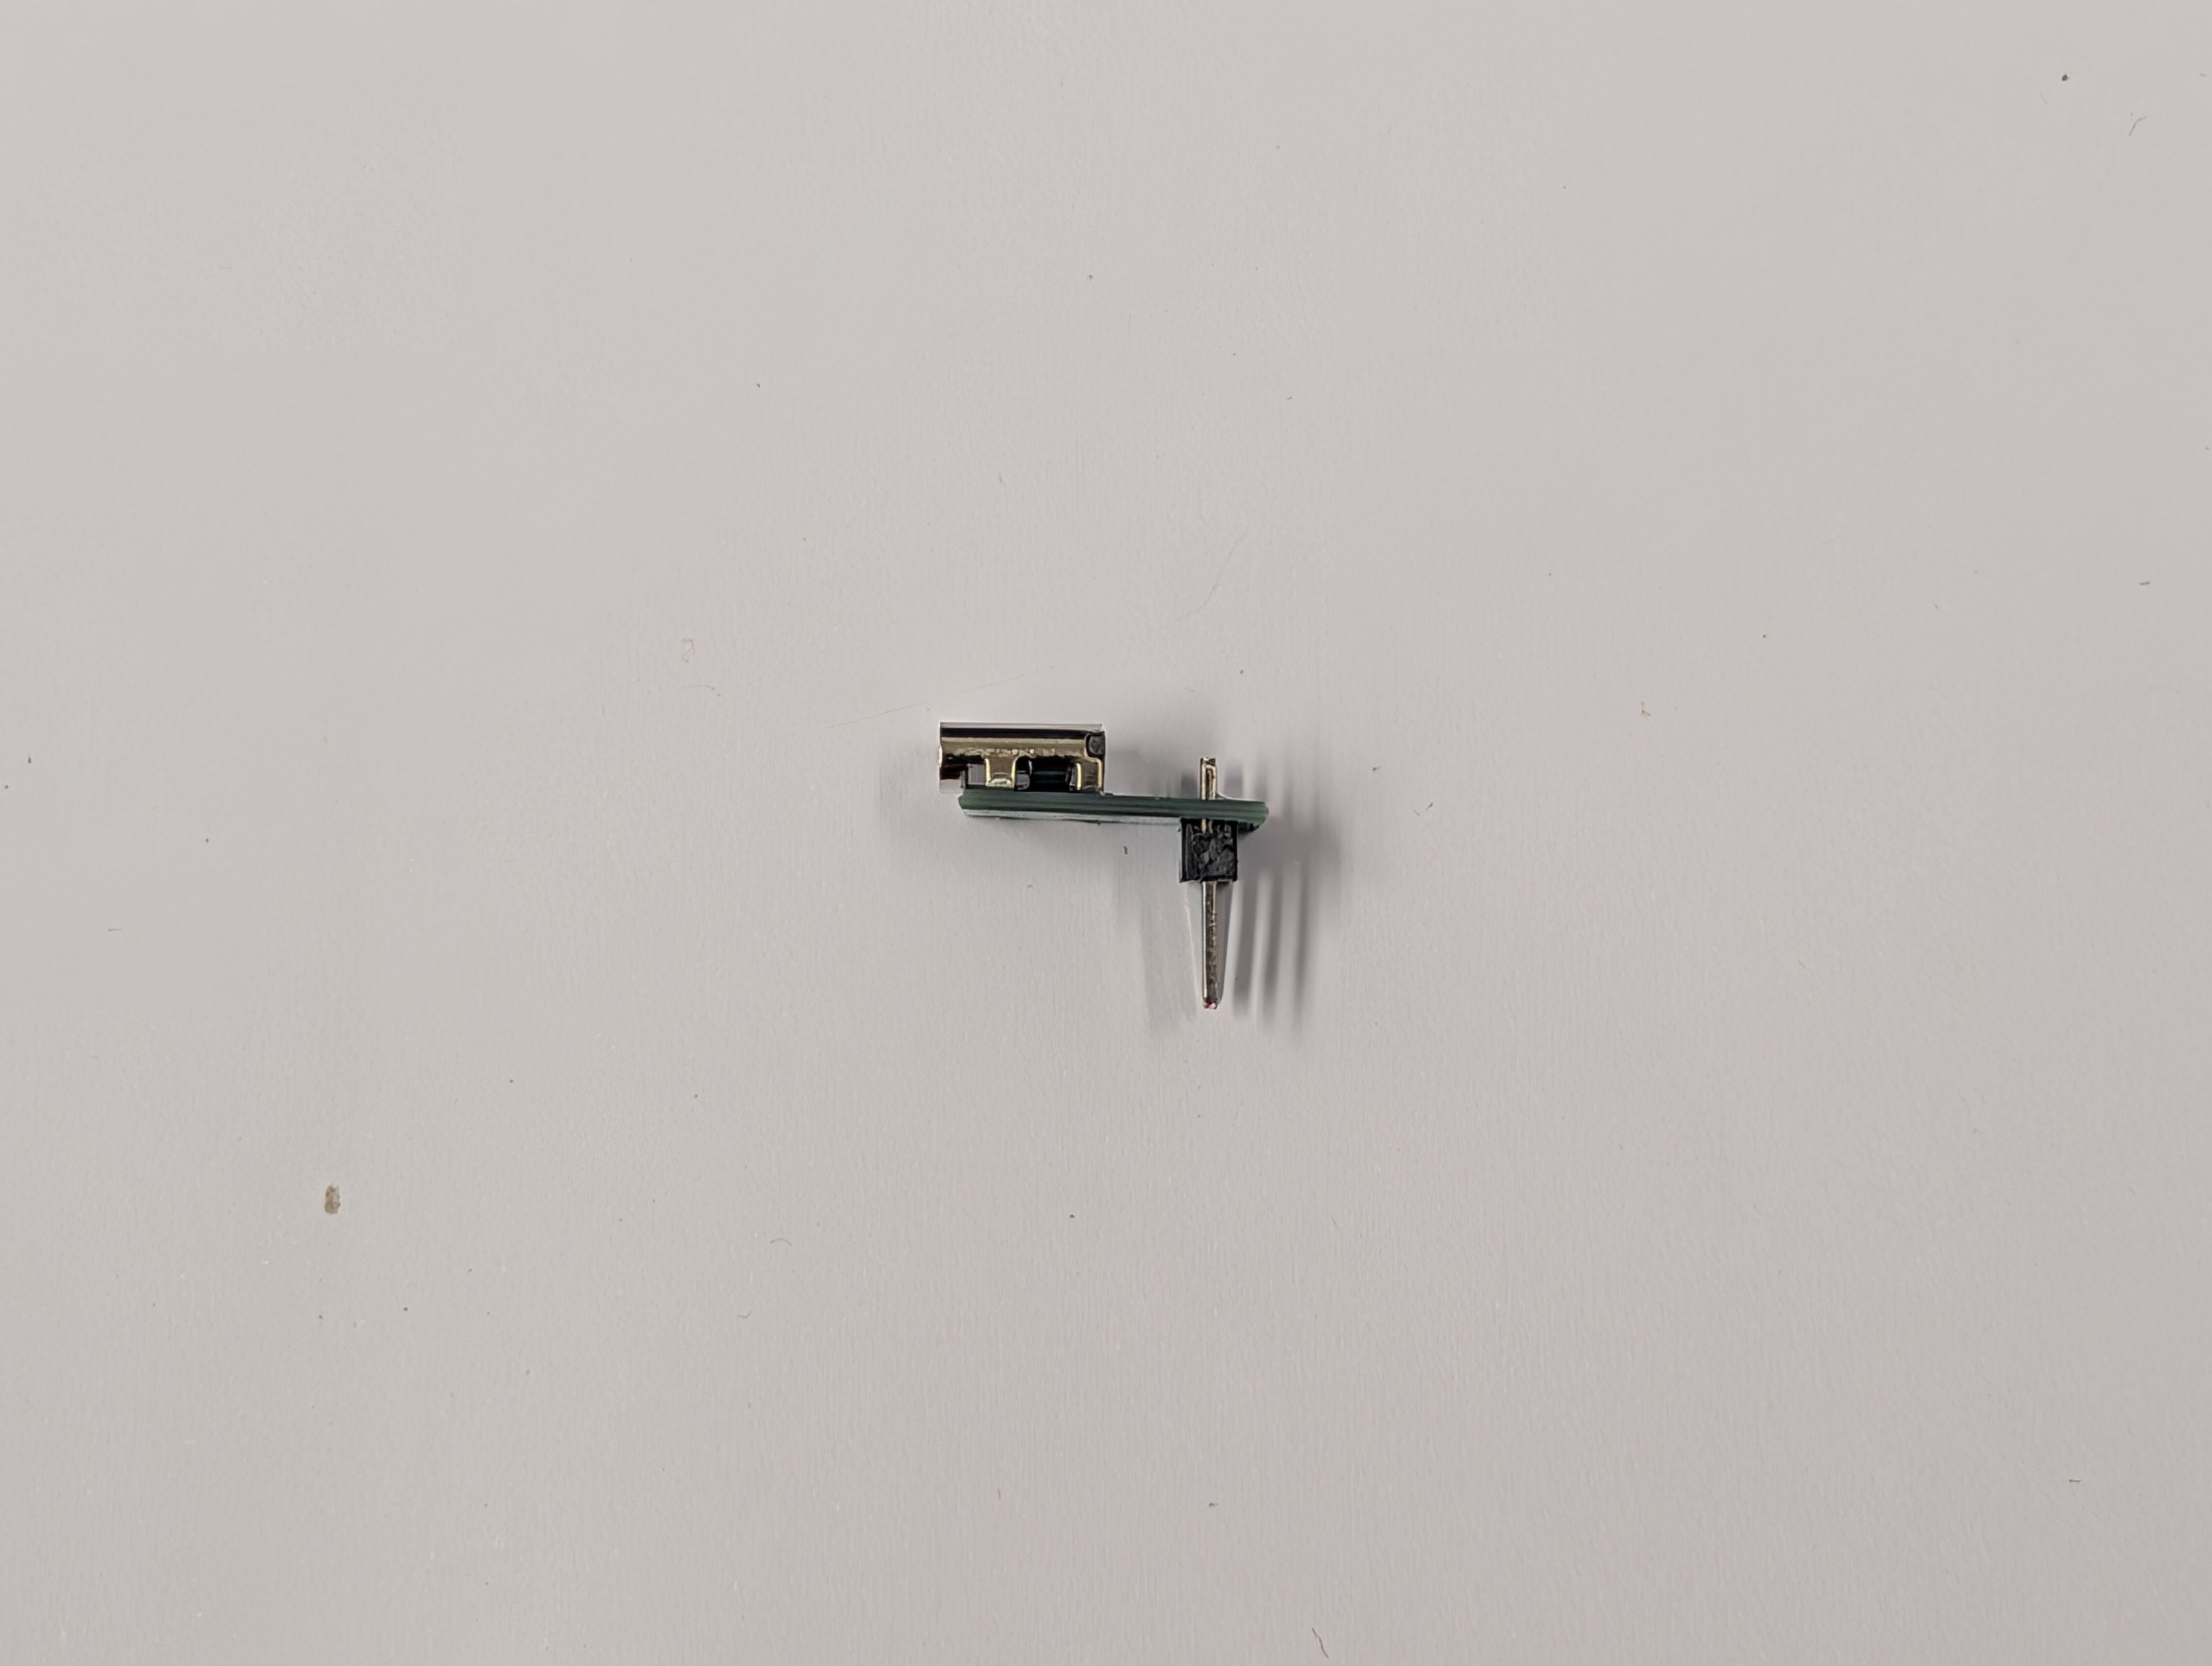
\includegraphics[width=0.75\textwidth]{pictures_of_construction/instruction_step_11.jpg}
\end{figure}

\subsection*{Assembly of the AHT10 digital temperature sensor}

\begin{figure}[H]
    \centering
    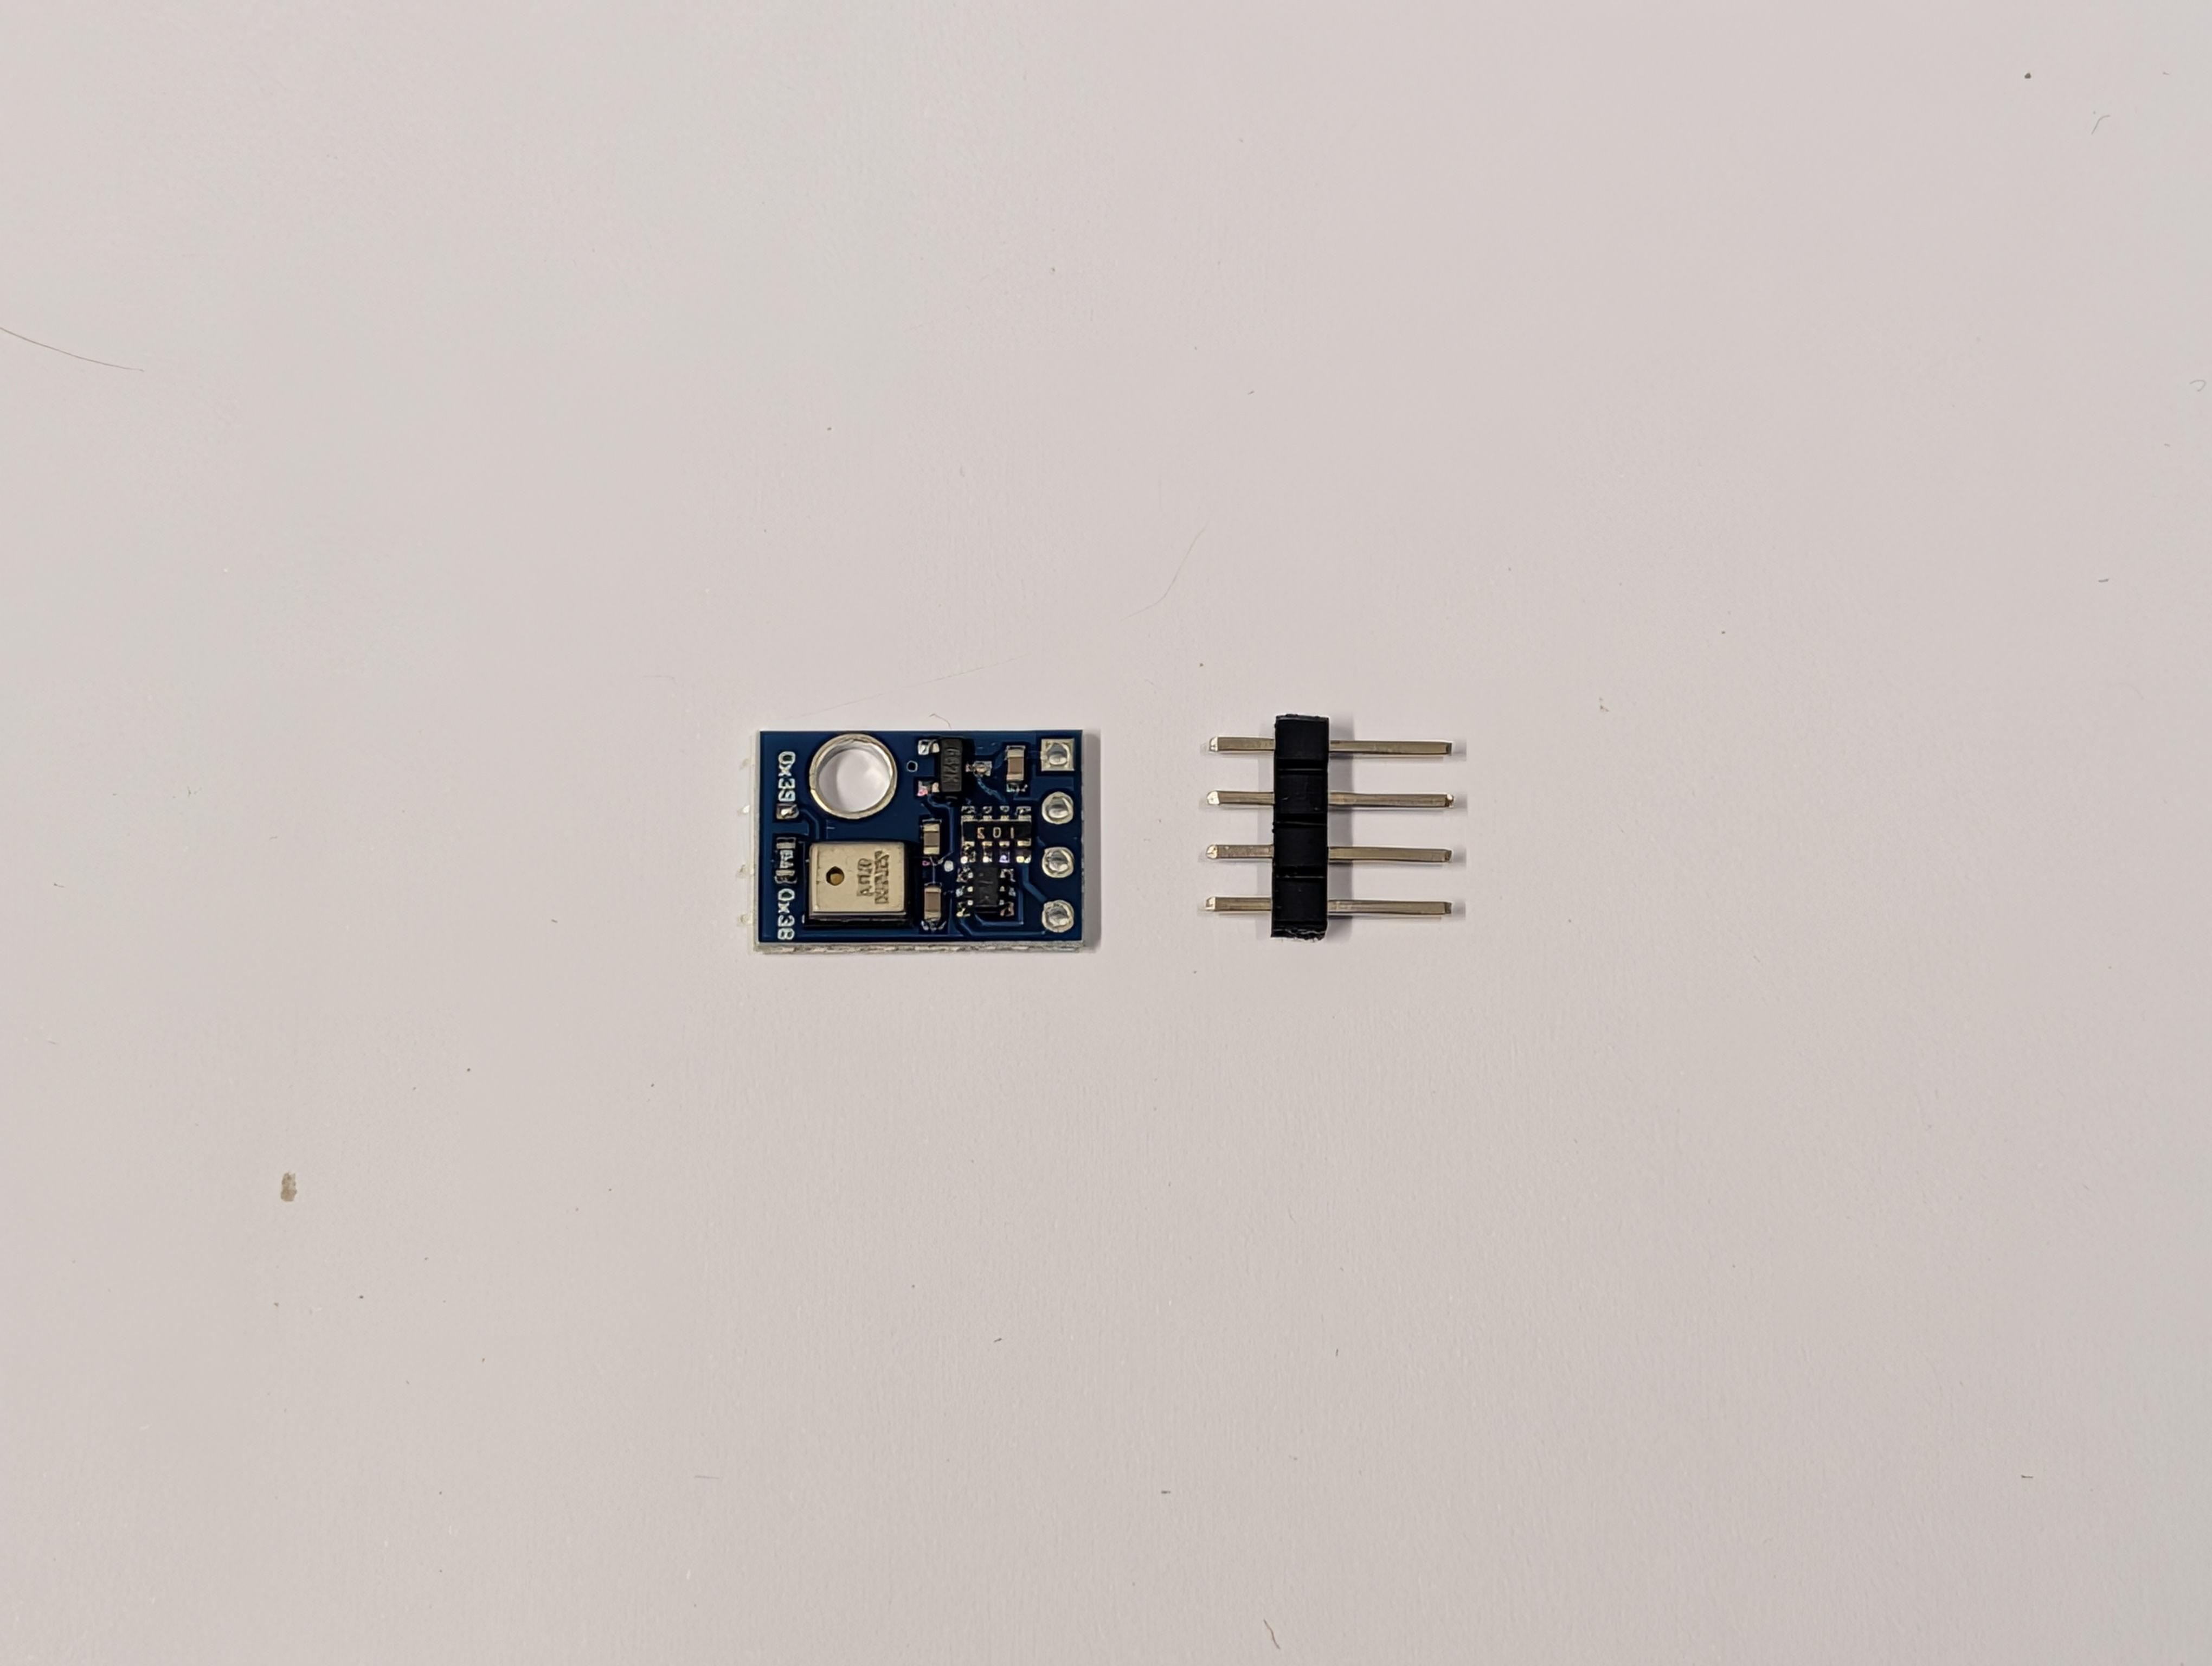
\includegraphics[width=0.75\textwidth]{pictures_of_construction/instruction_step_12.jpg}
\end{figure}

The assembly of the AHT10 digital temperature sensor is identical to that of the USB-C breakout board. Start by soldering only one pin and correct the alignment so it is nice and perpendicular.

\begin{figure}[H]
    \centering
    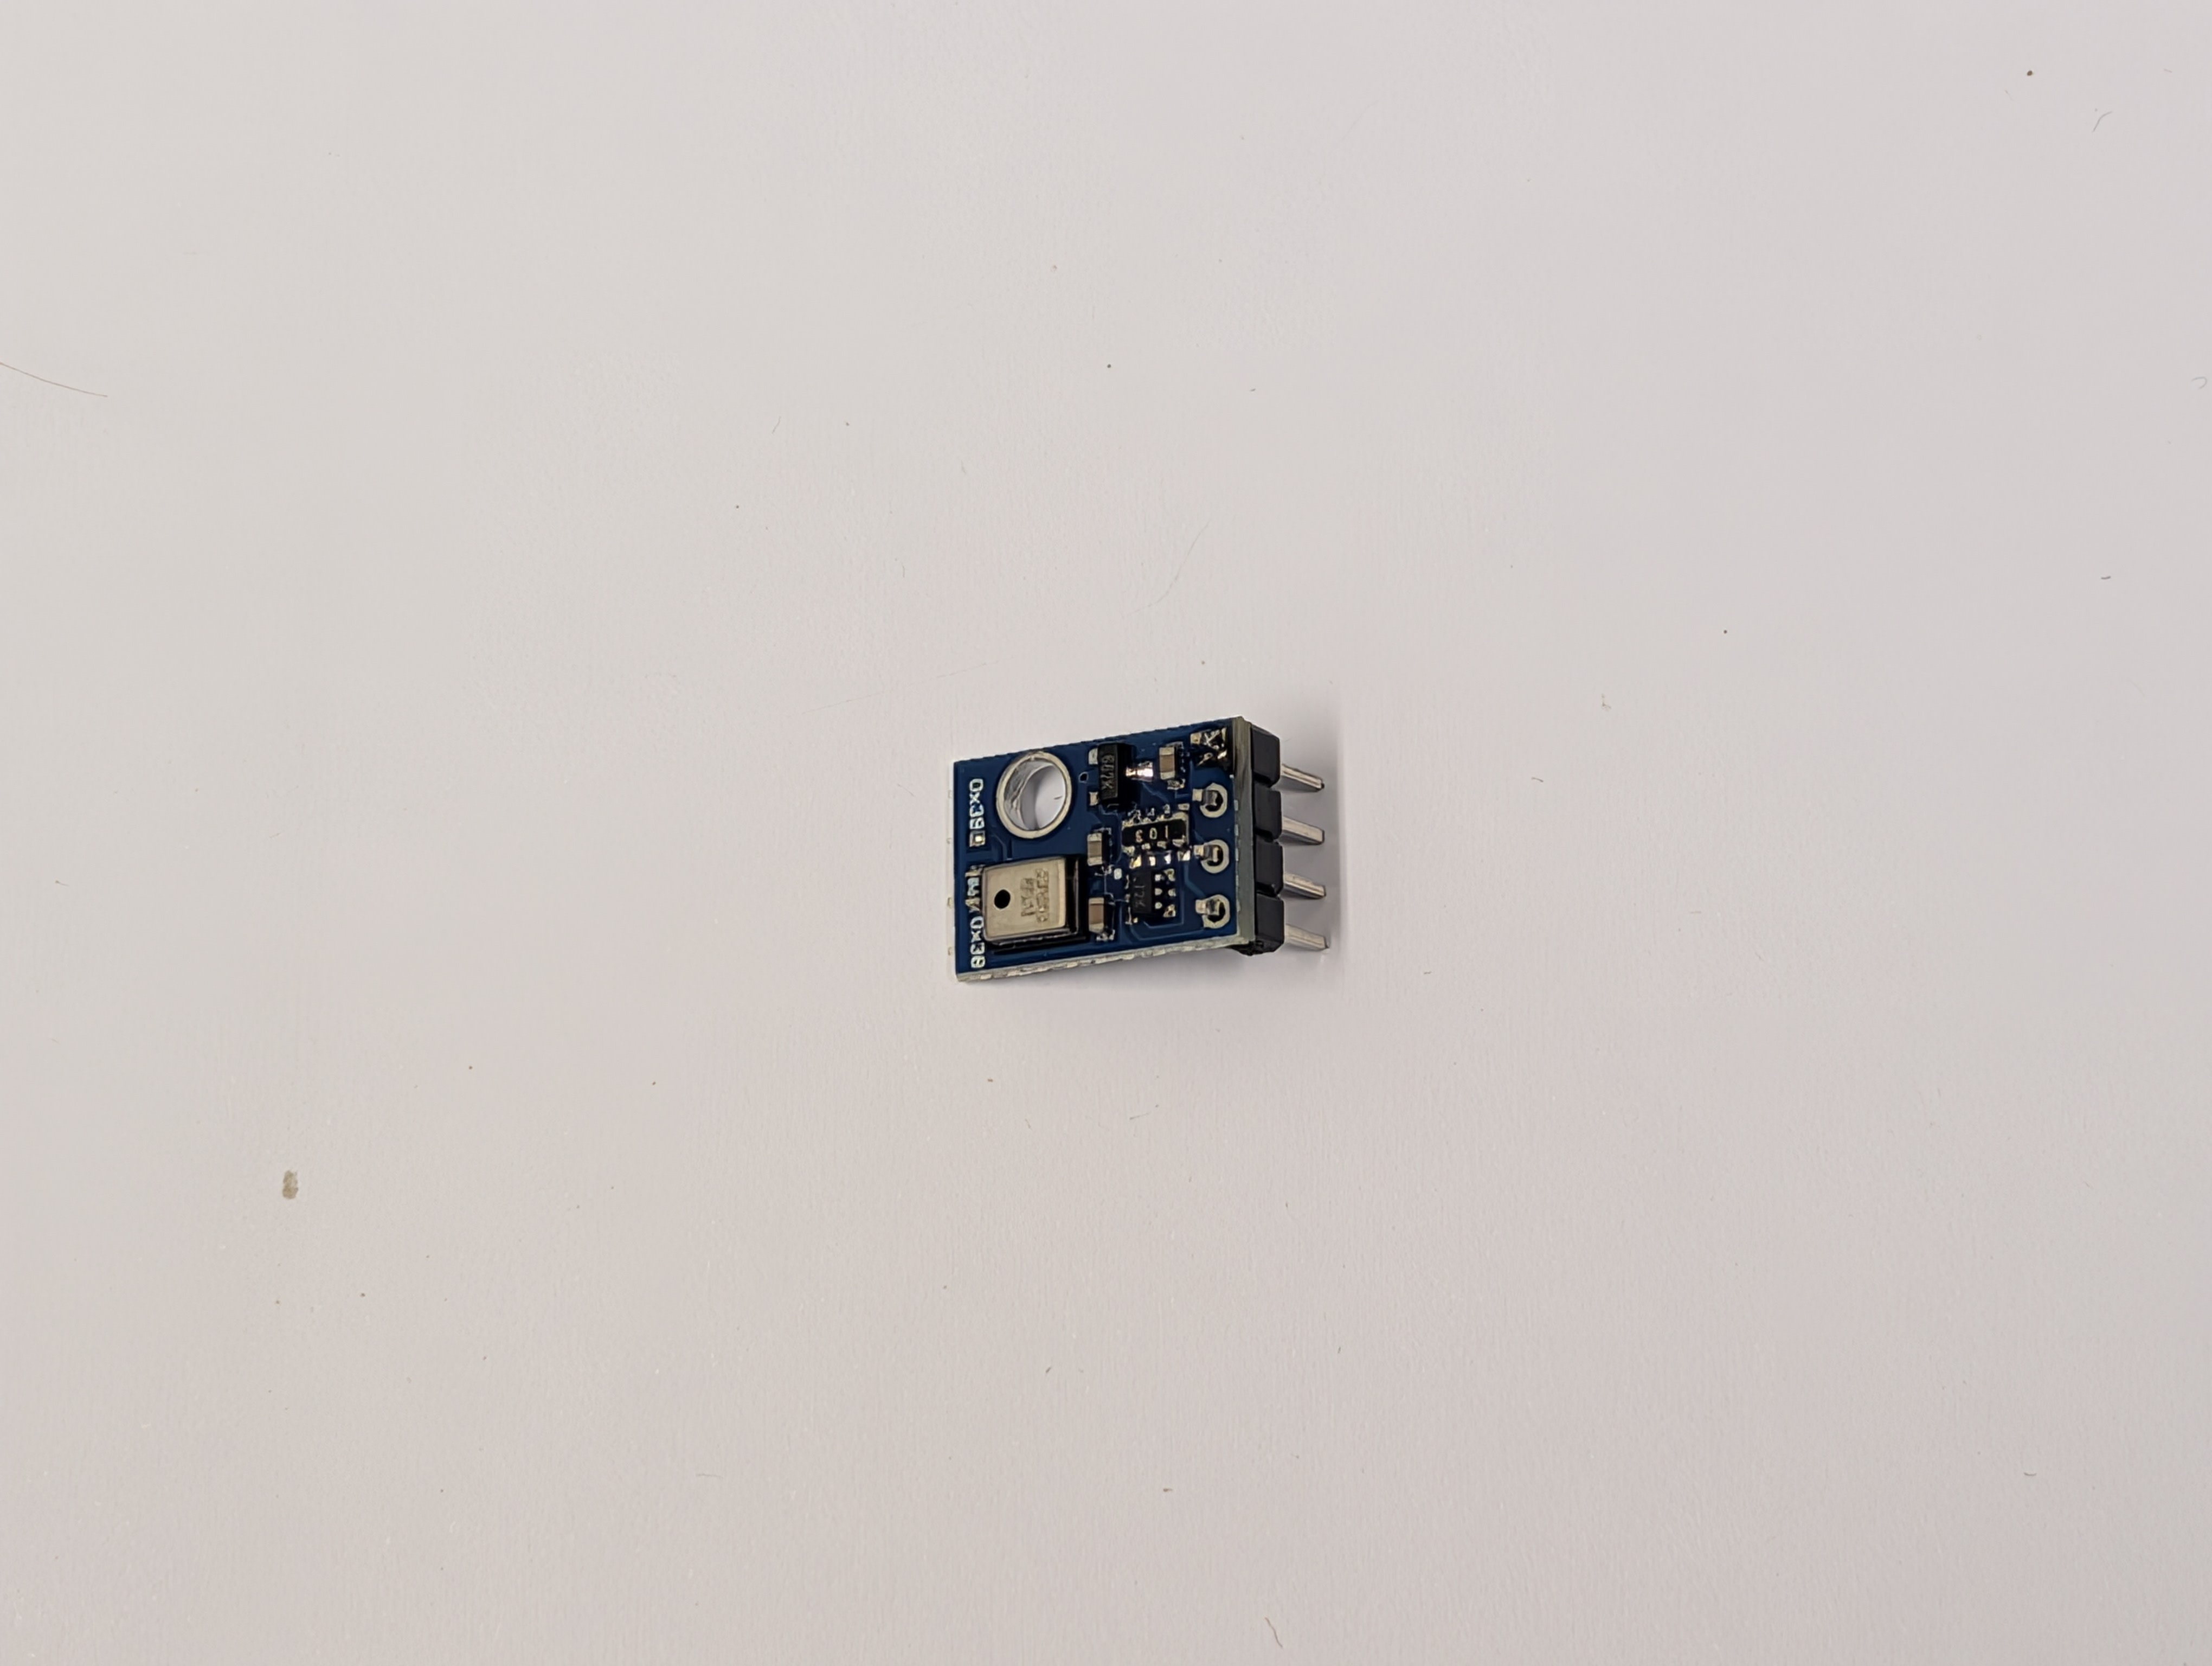
\includegraphics[width=0.75\textwidth]{pictures_of_construction/instruction_step_13.jpg}
\end{figure}

\subsection*{Assembly of the 1602A LCD display}

\begin{figure}[H]
    \centering
    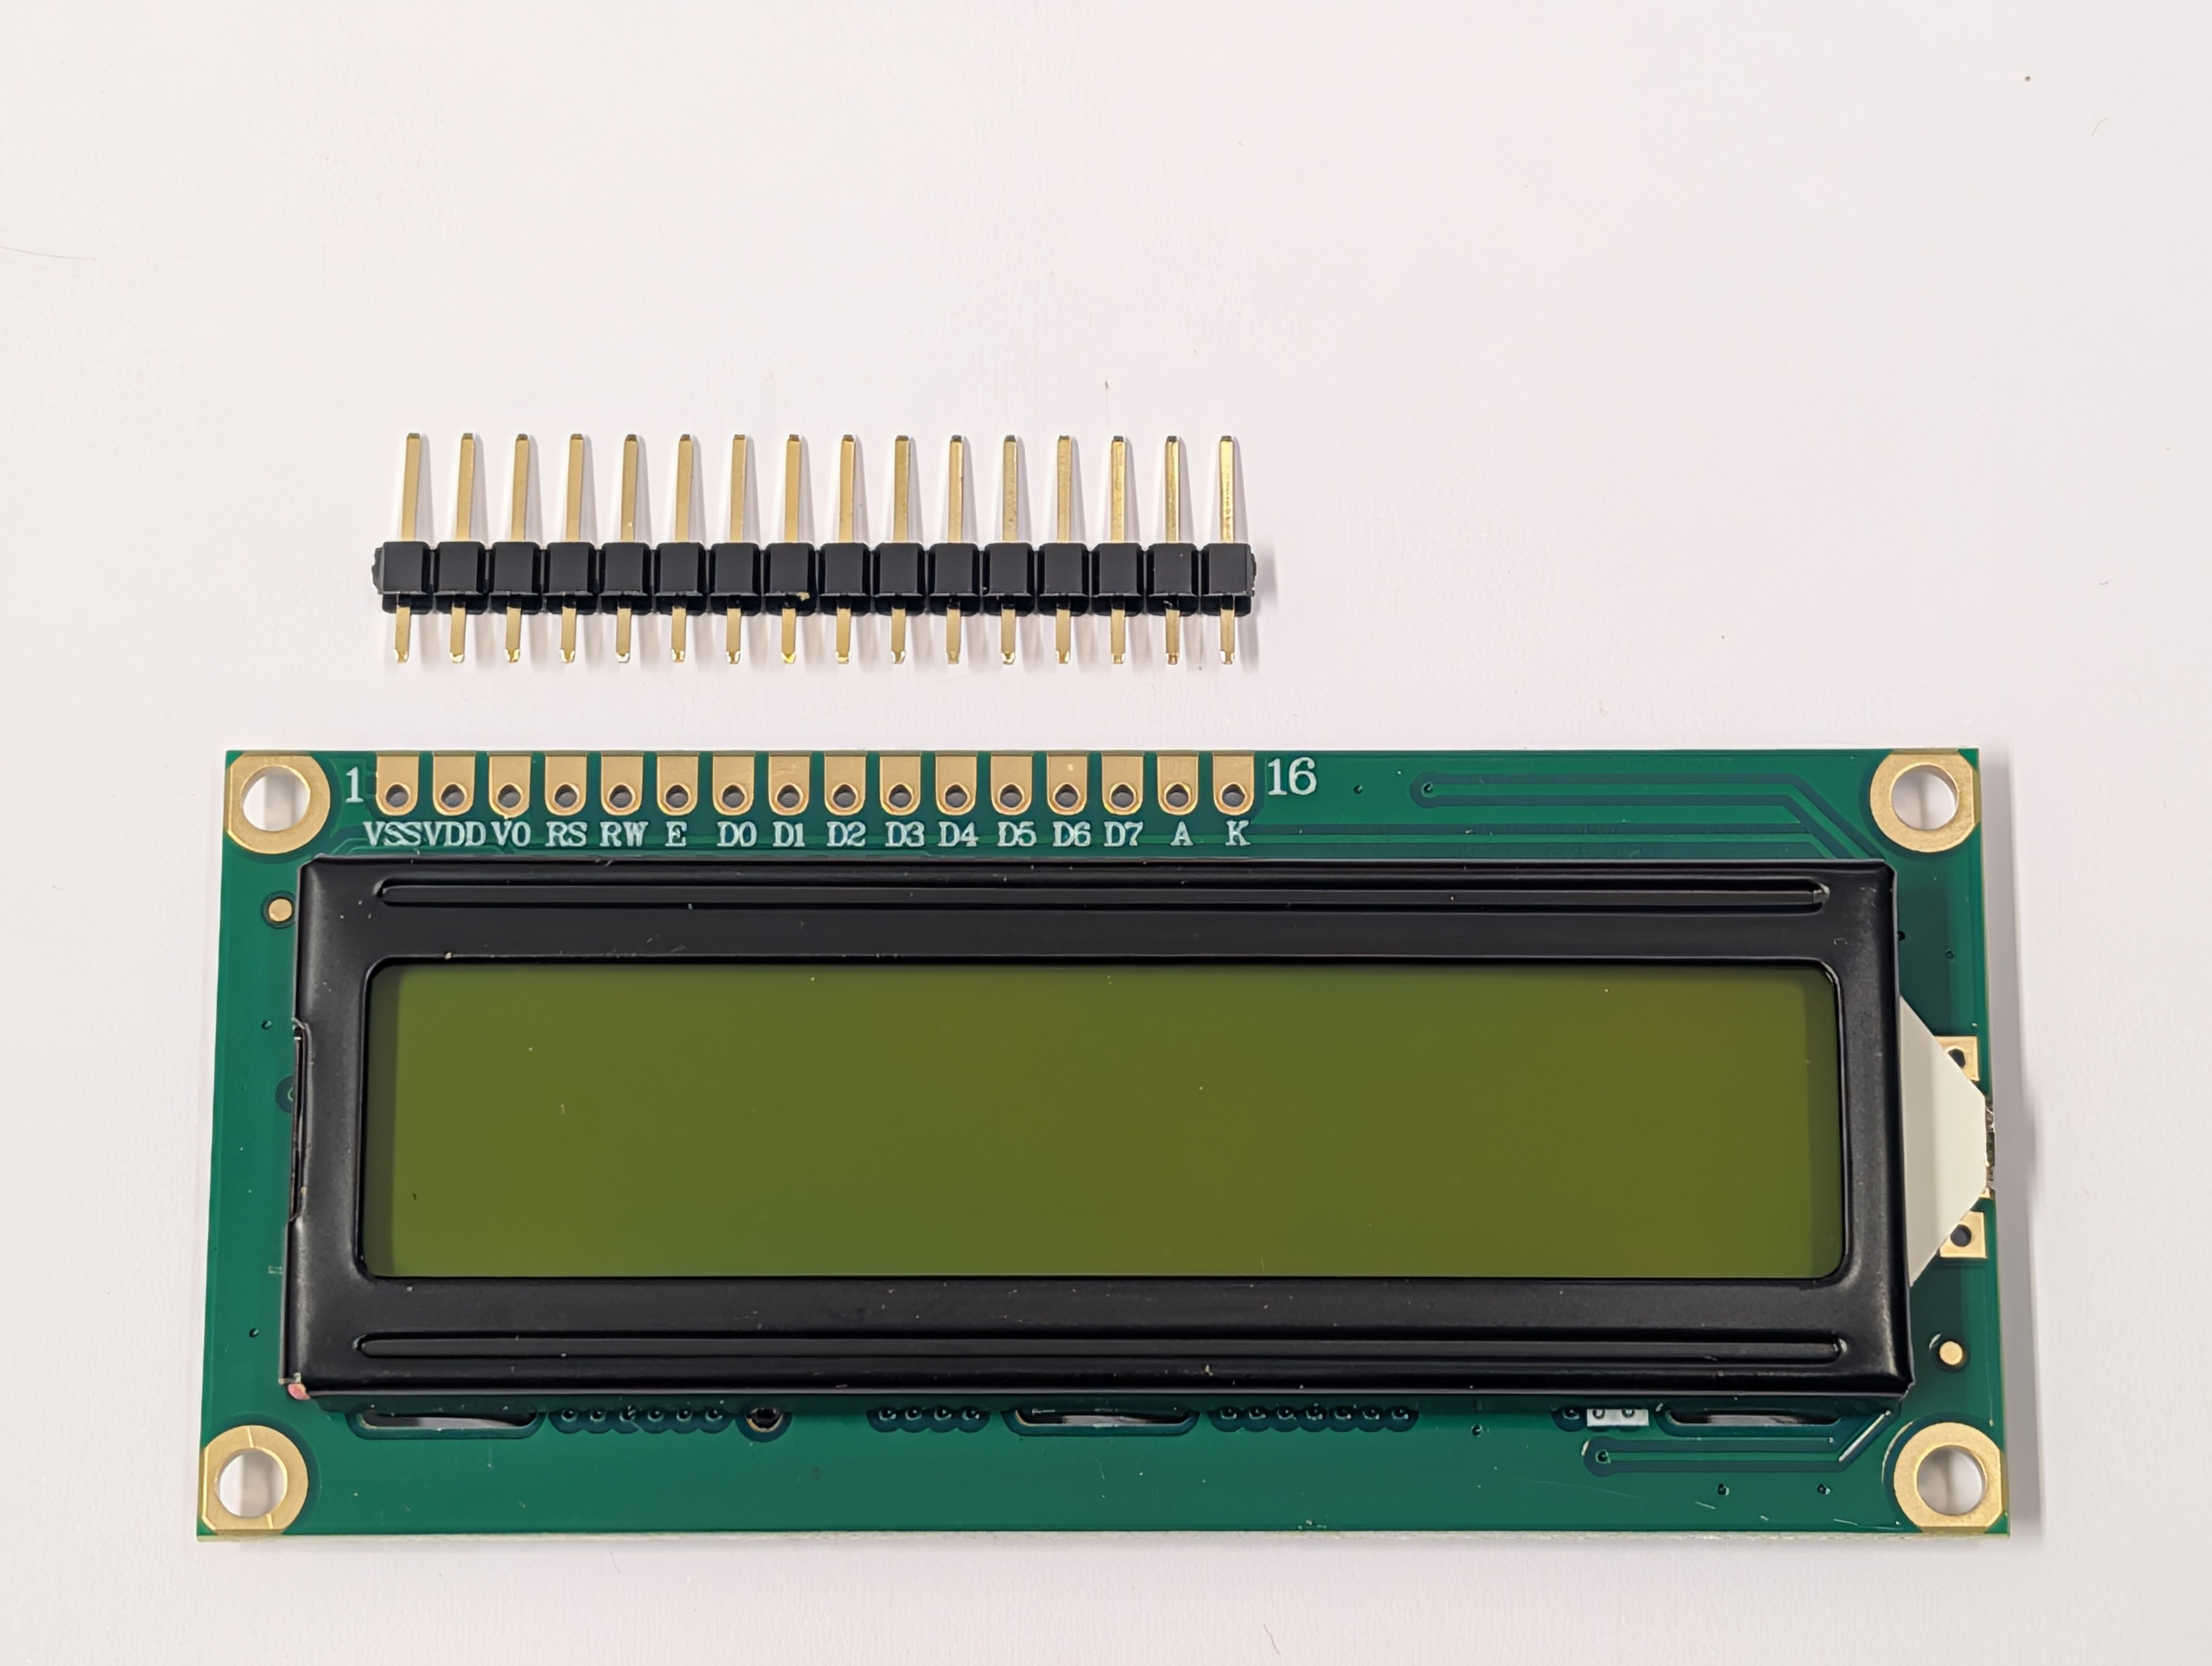
\includegraphics[width=0.75\textwidth]{pictures_of_construction/instruction_step_14.jpg}
\end{figure}

The assembly of the 1602A LCD display is very similar to the previous two steps. First solder one pin, check for squareness and correct, then solder all pins.

\begin{figure}[H]
    \centering
    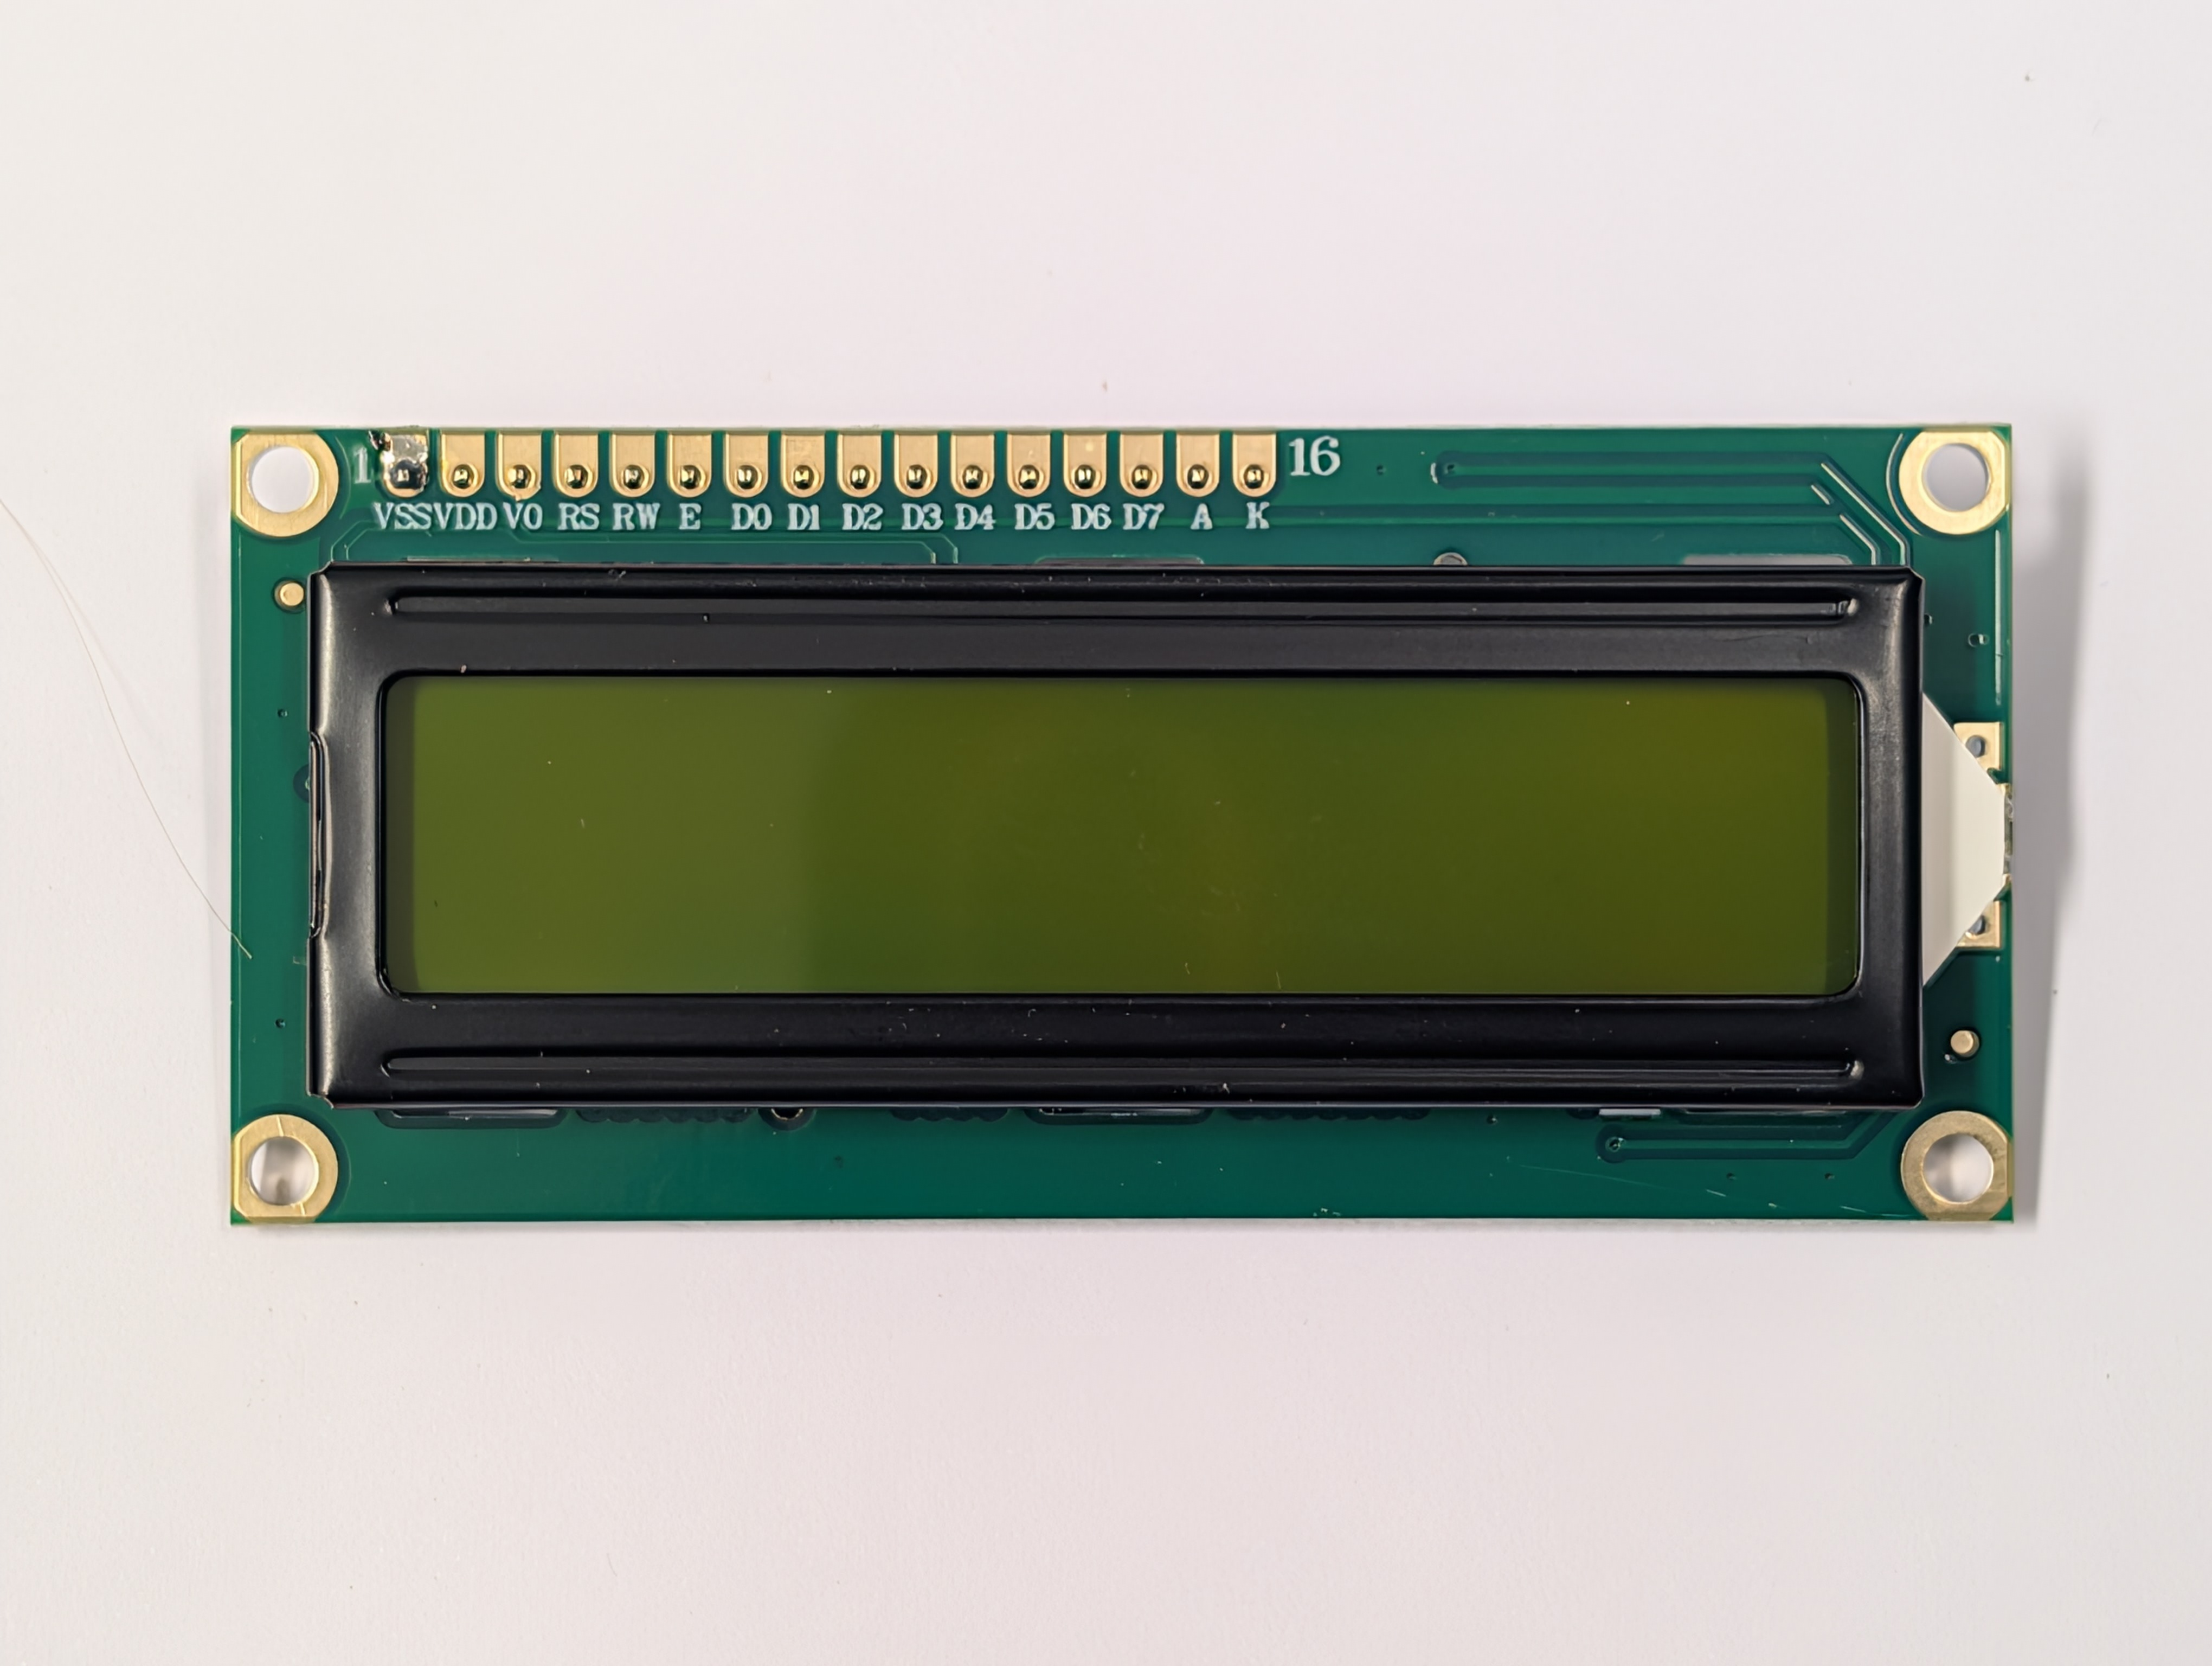
\includegraphics[width=0.75\textwidth]{pictures_of_construction/instruction_step_15.jpg}
\end{figure}

\begin{figure}[H]
    \centering
    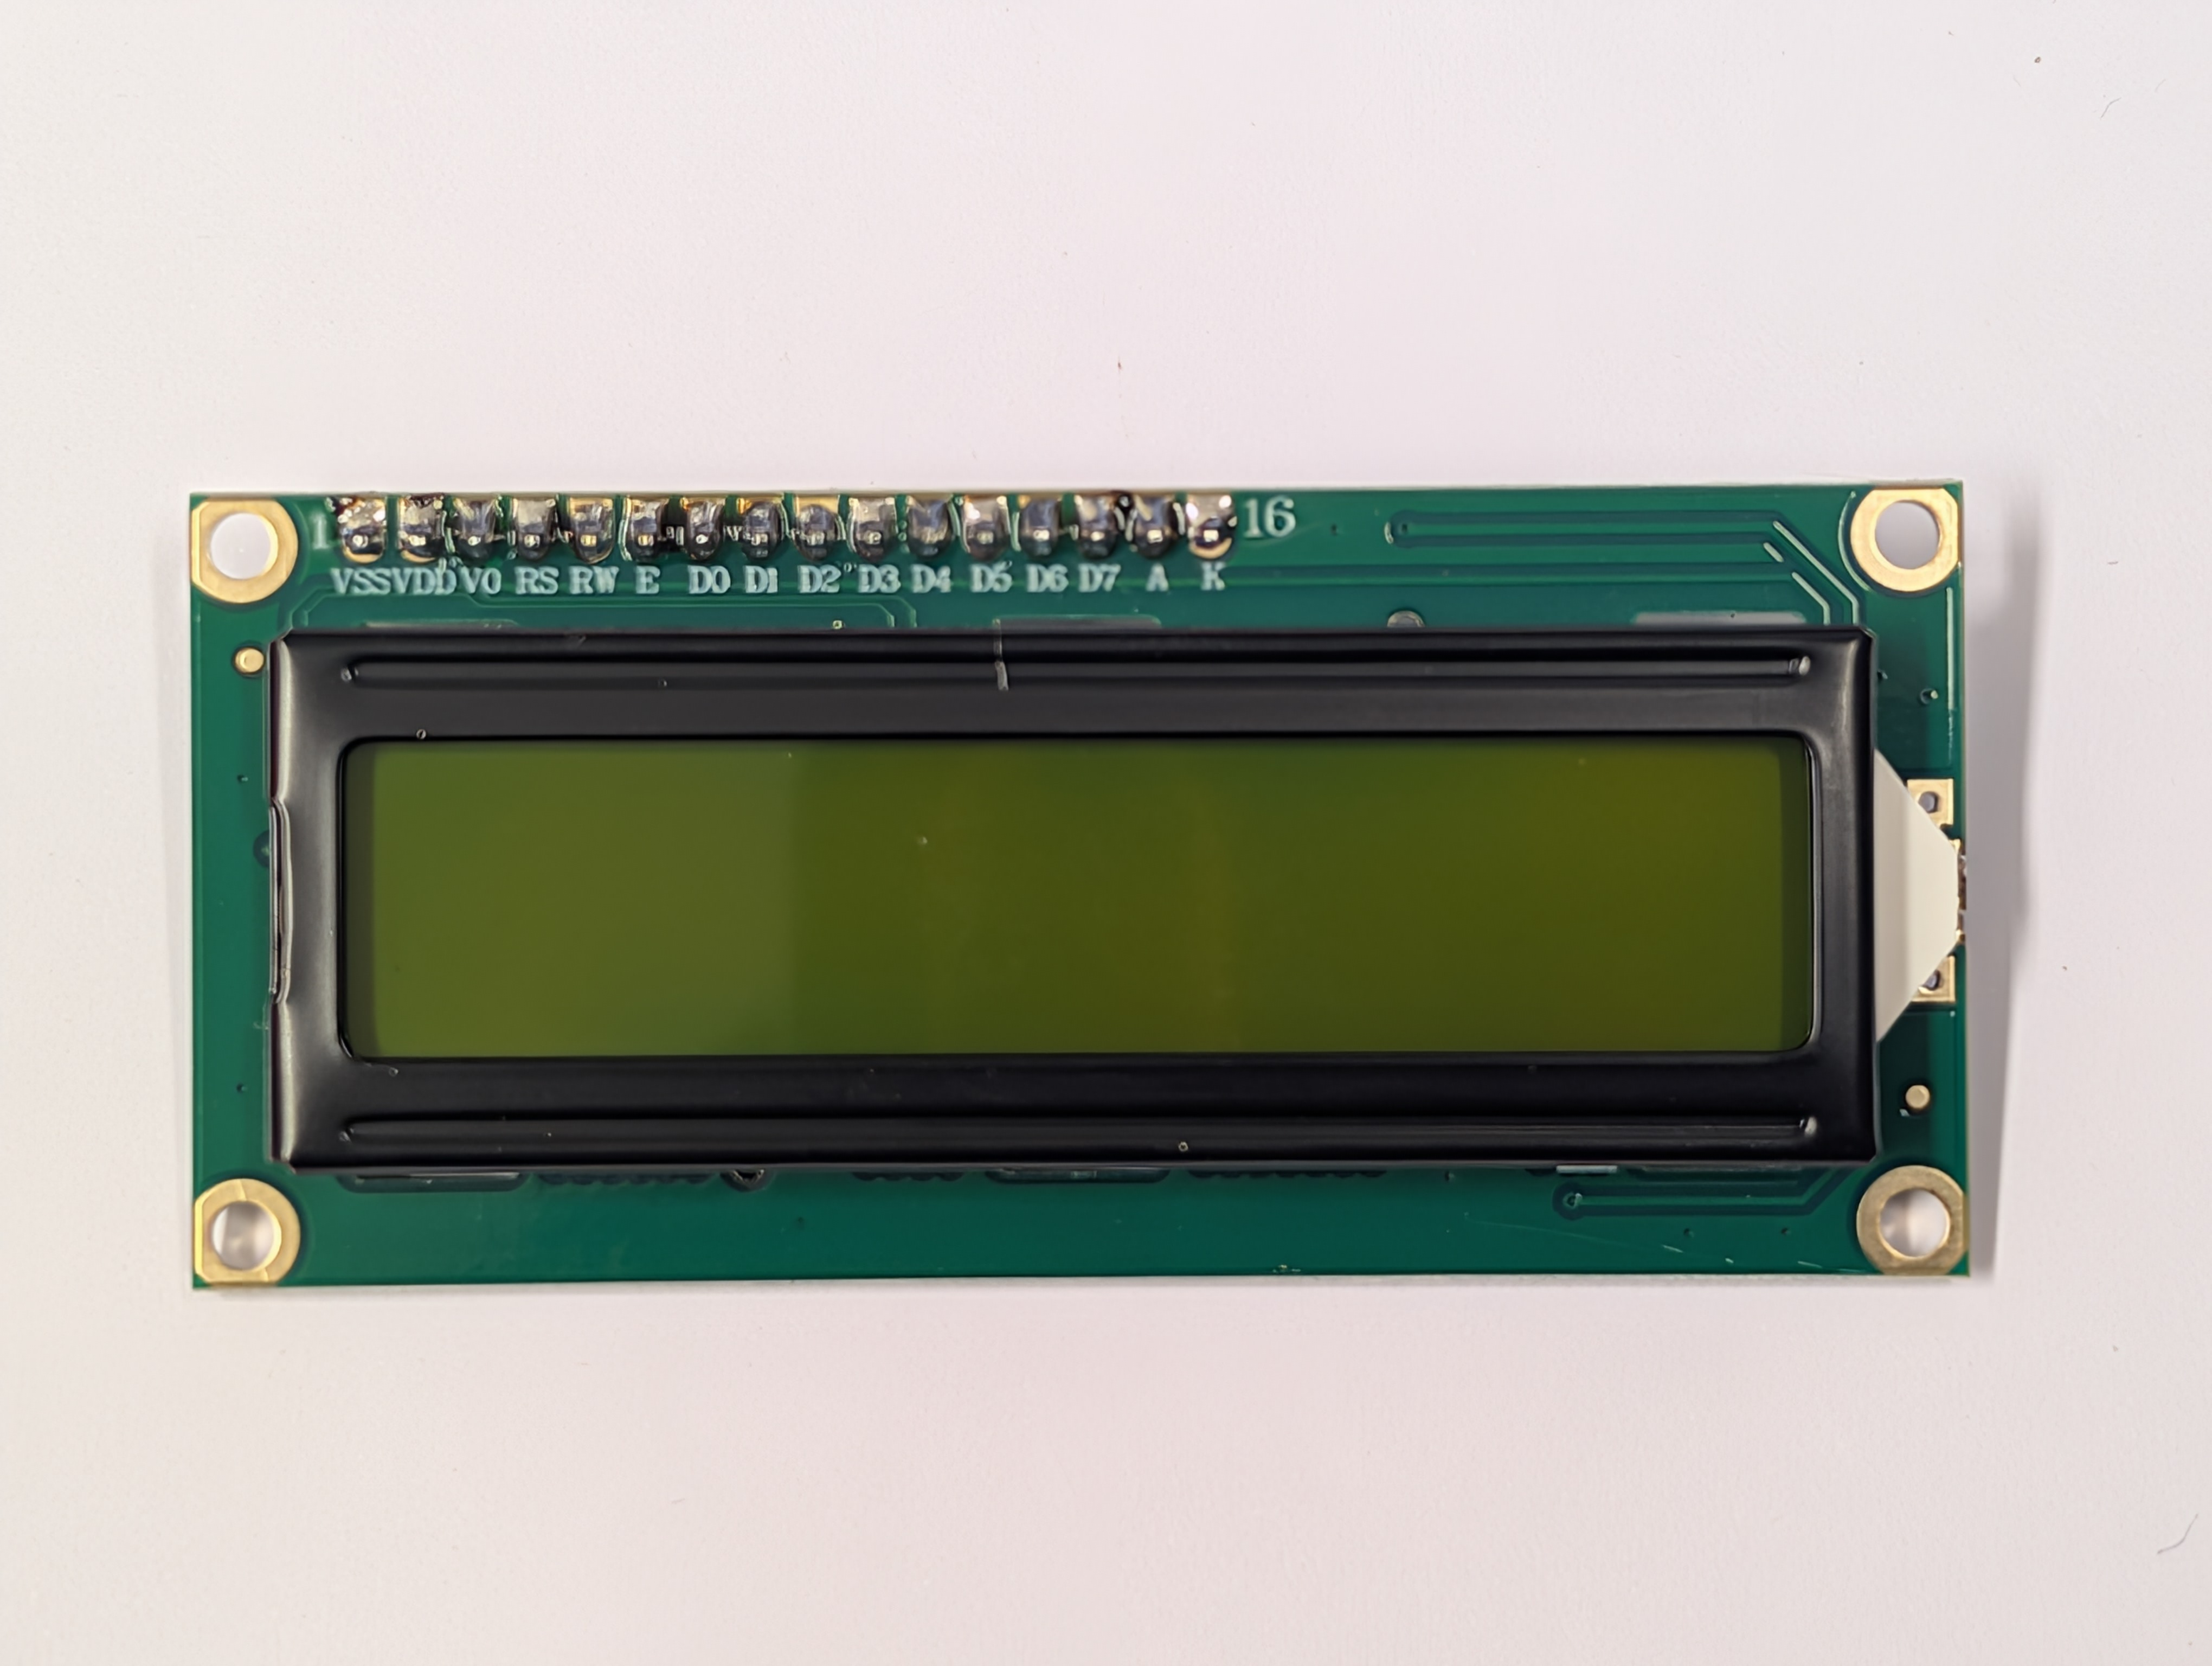
\includegraphics[width=0.75\textwidth]{pictures_of_construction/instruction_step_16.jpg}
\end{figure}

\subsection*{Installation of resistors}

\subsubsection*{100 k$\Omega$ NTC temperature-dependent resistor}

The 100 k$\Omega$ NTC temperature-dependent resistor has a glass body with no markings.

\begin{figure}[H]
    \centering
    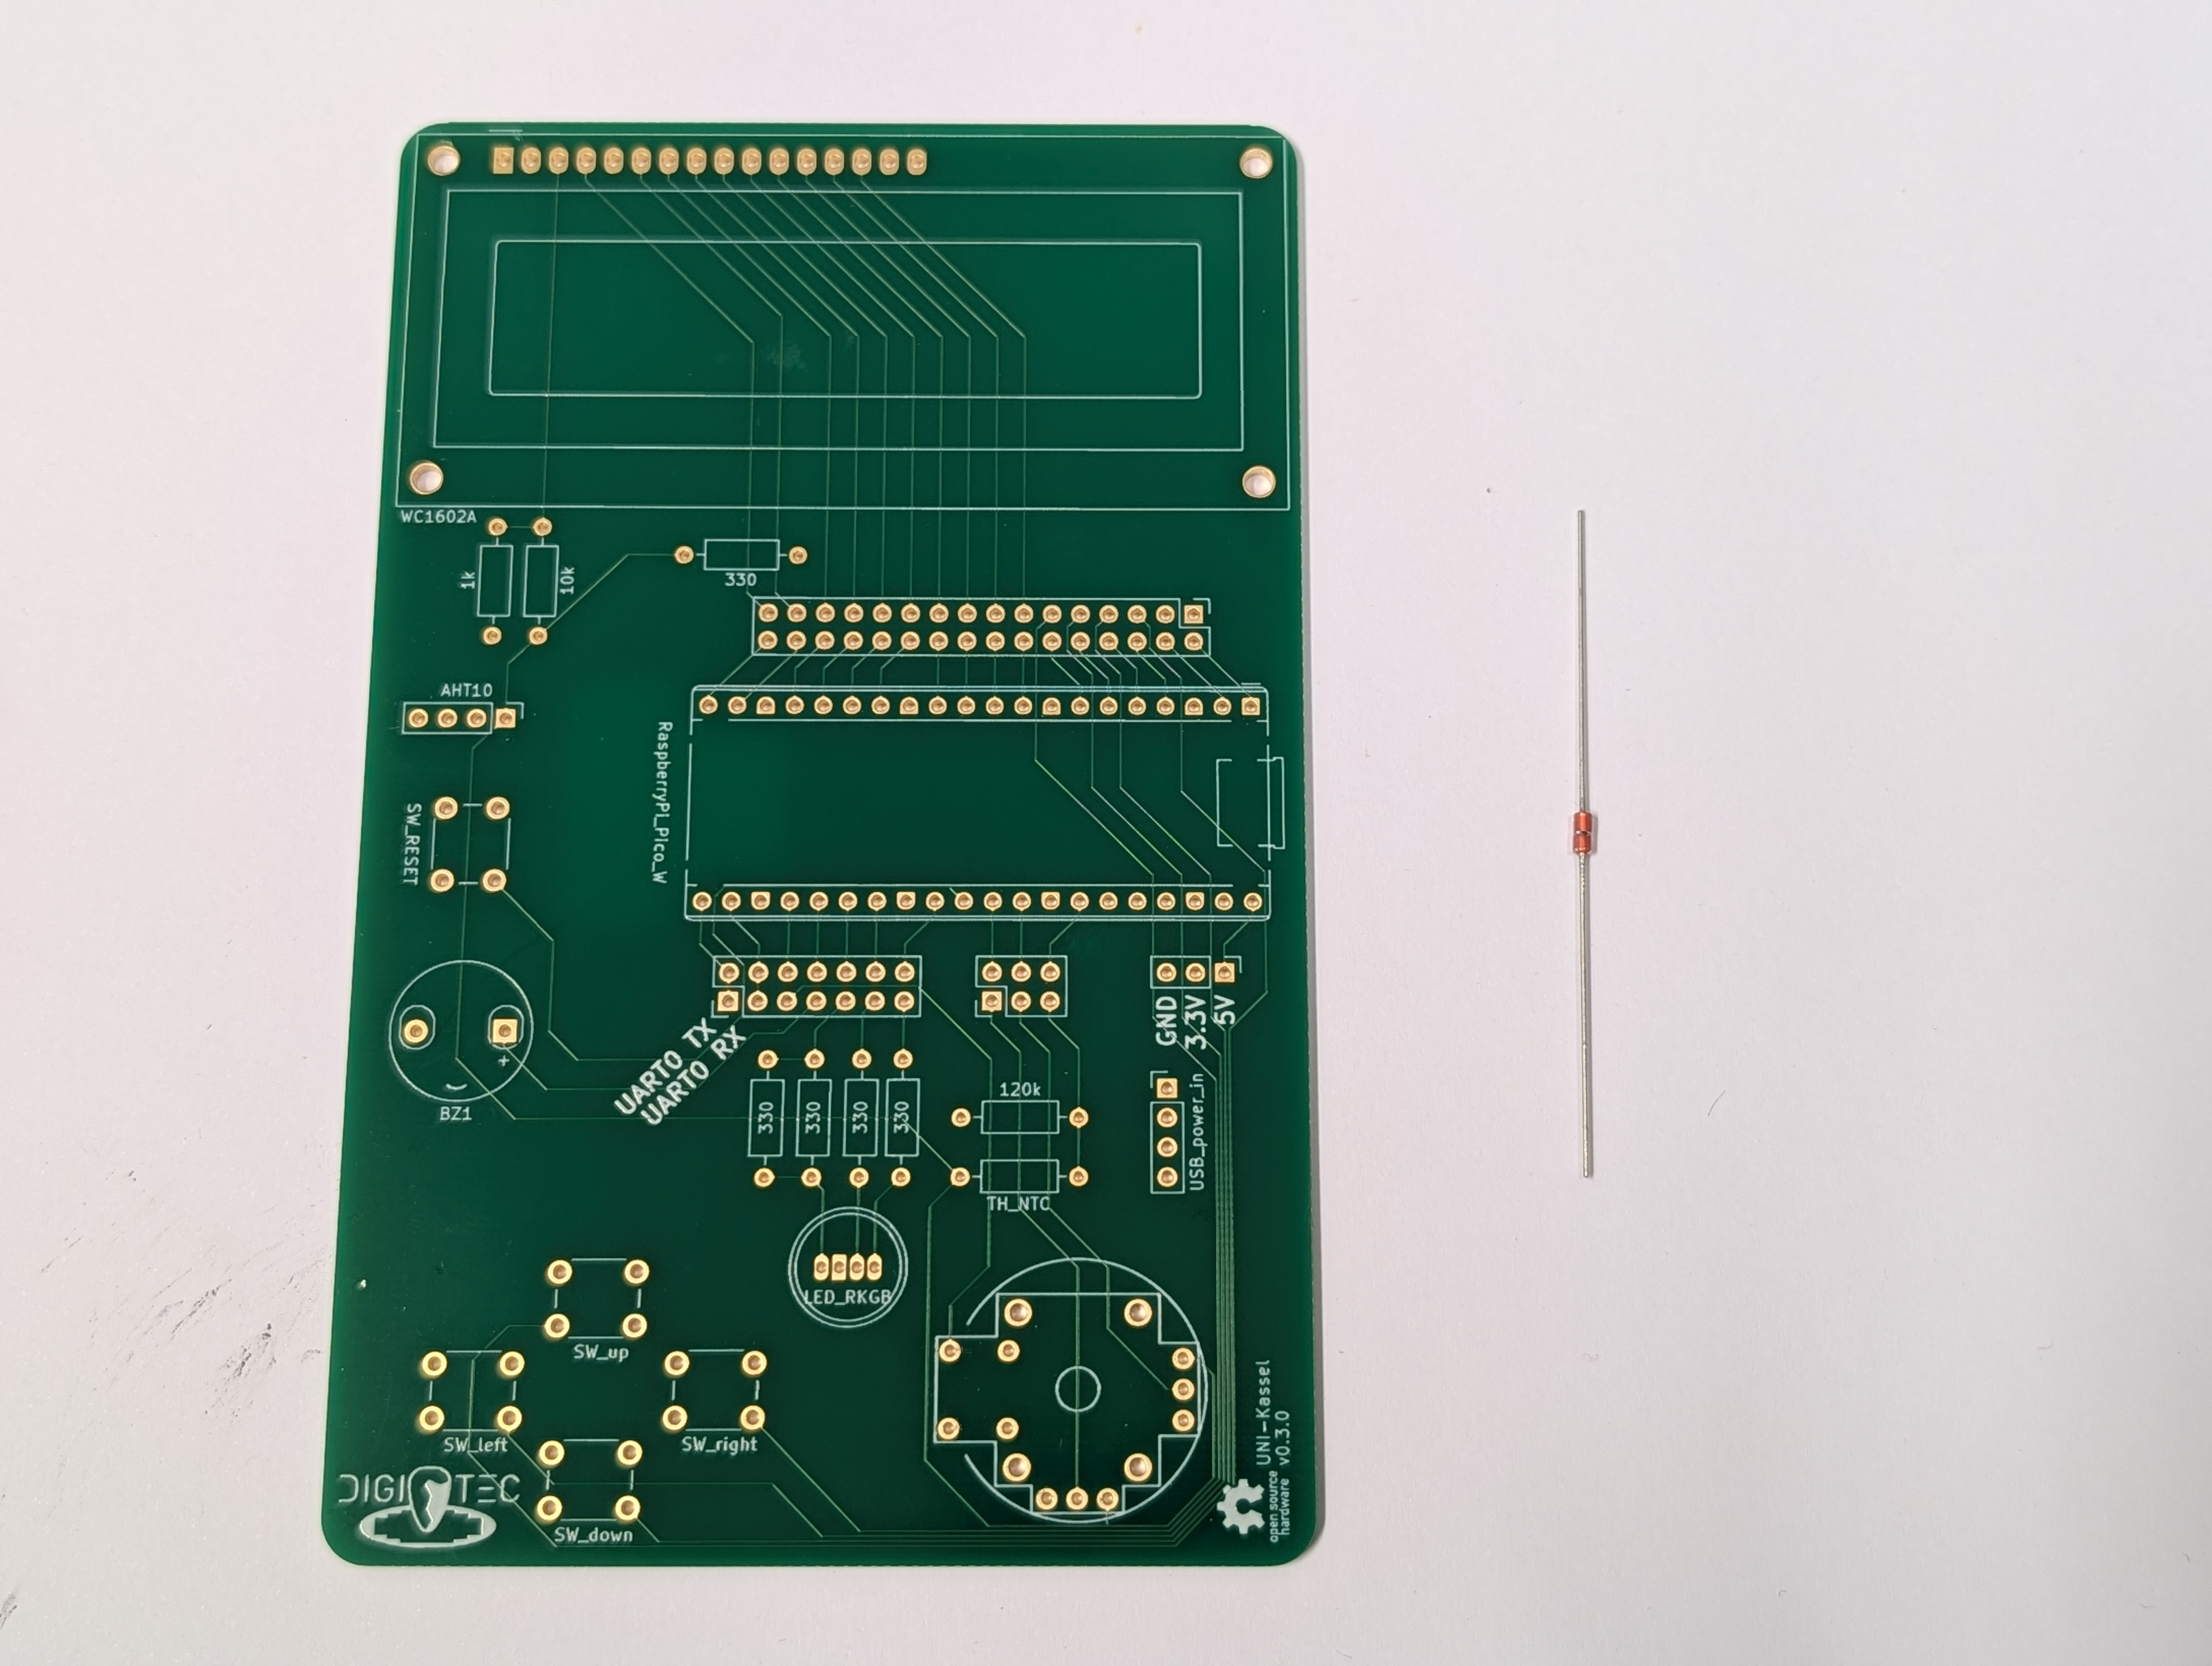
\includegraphics[width=0.75\textwidth]{pictures_of_construction/instruction_step_17.jpg}
\end{figure}

The resistors come with straight leads and need to be formed. For that purpose hold them with one hand between two fingers and pull them to a U-shape with your other hand as seen in the following pictures:

\begin{figure}[H]
    \centering
    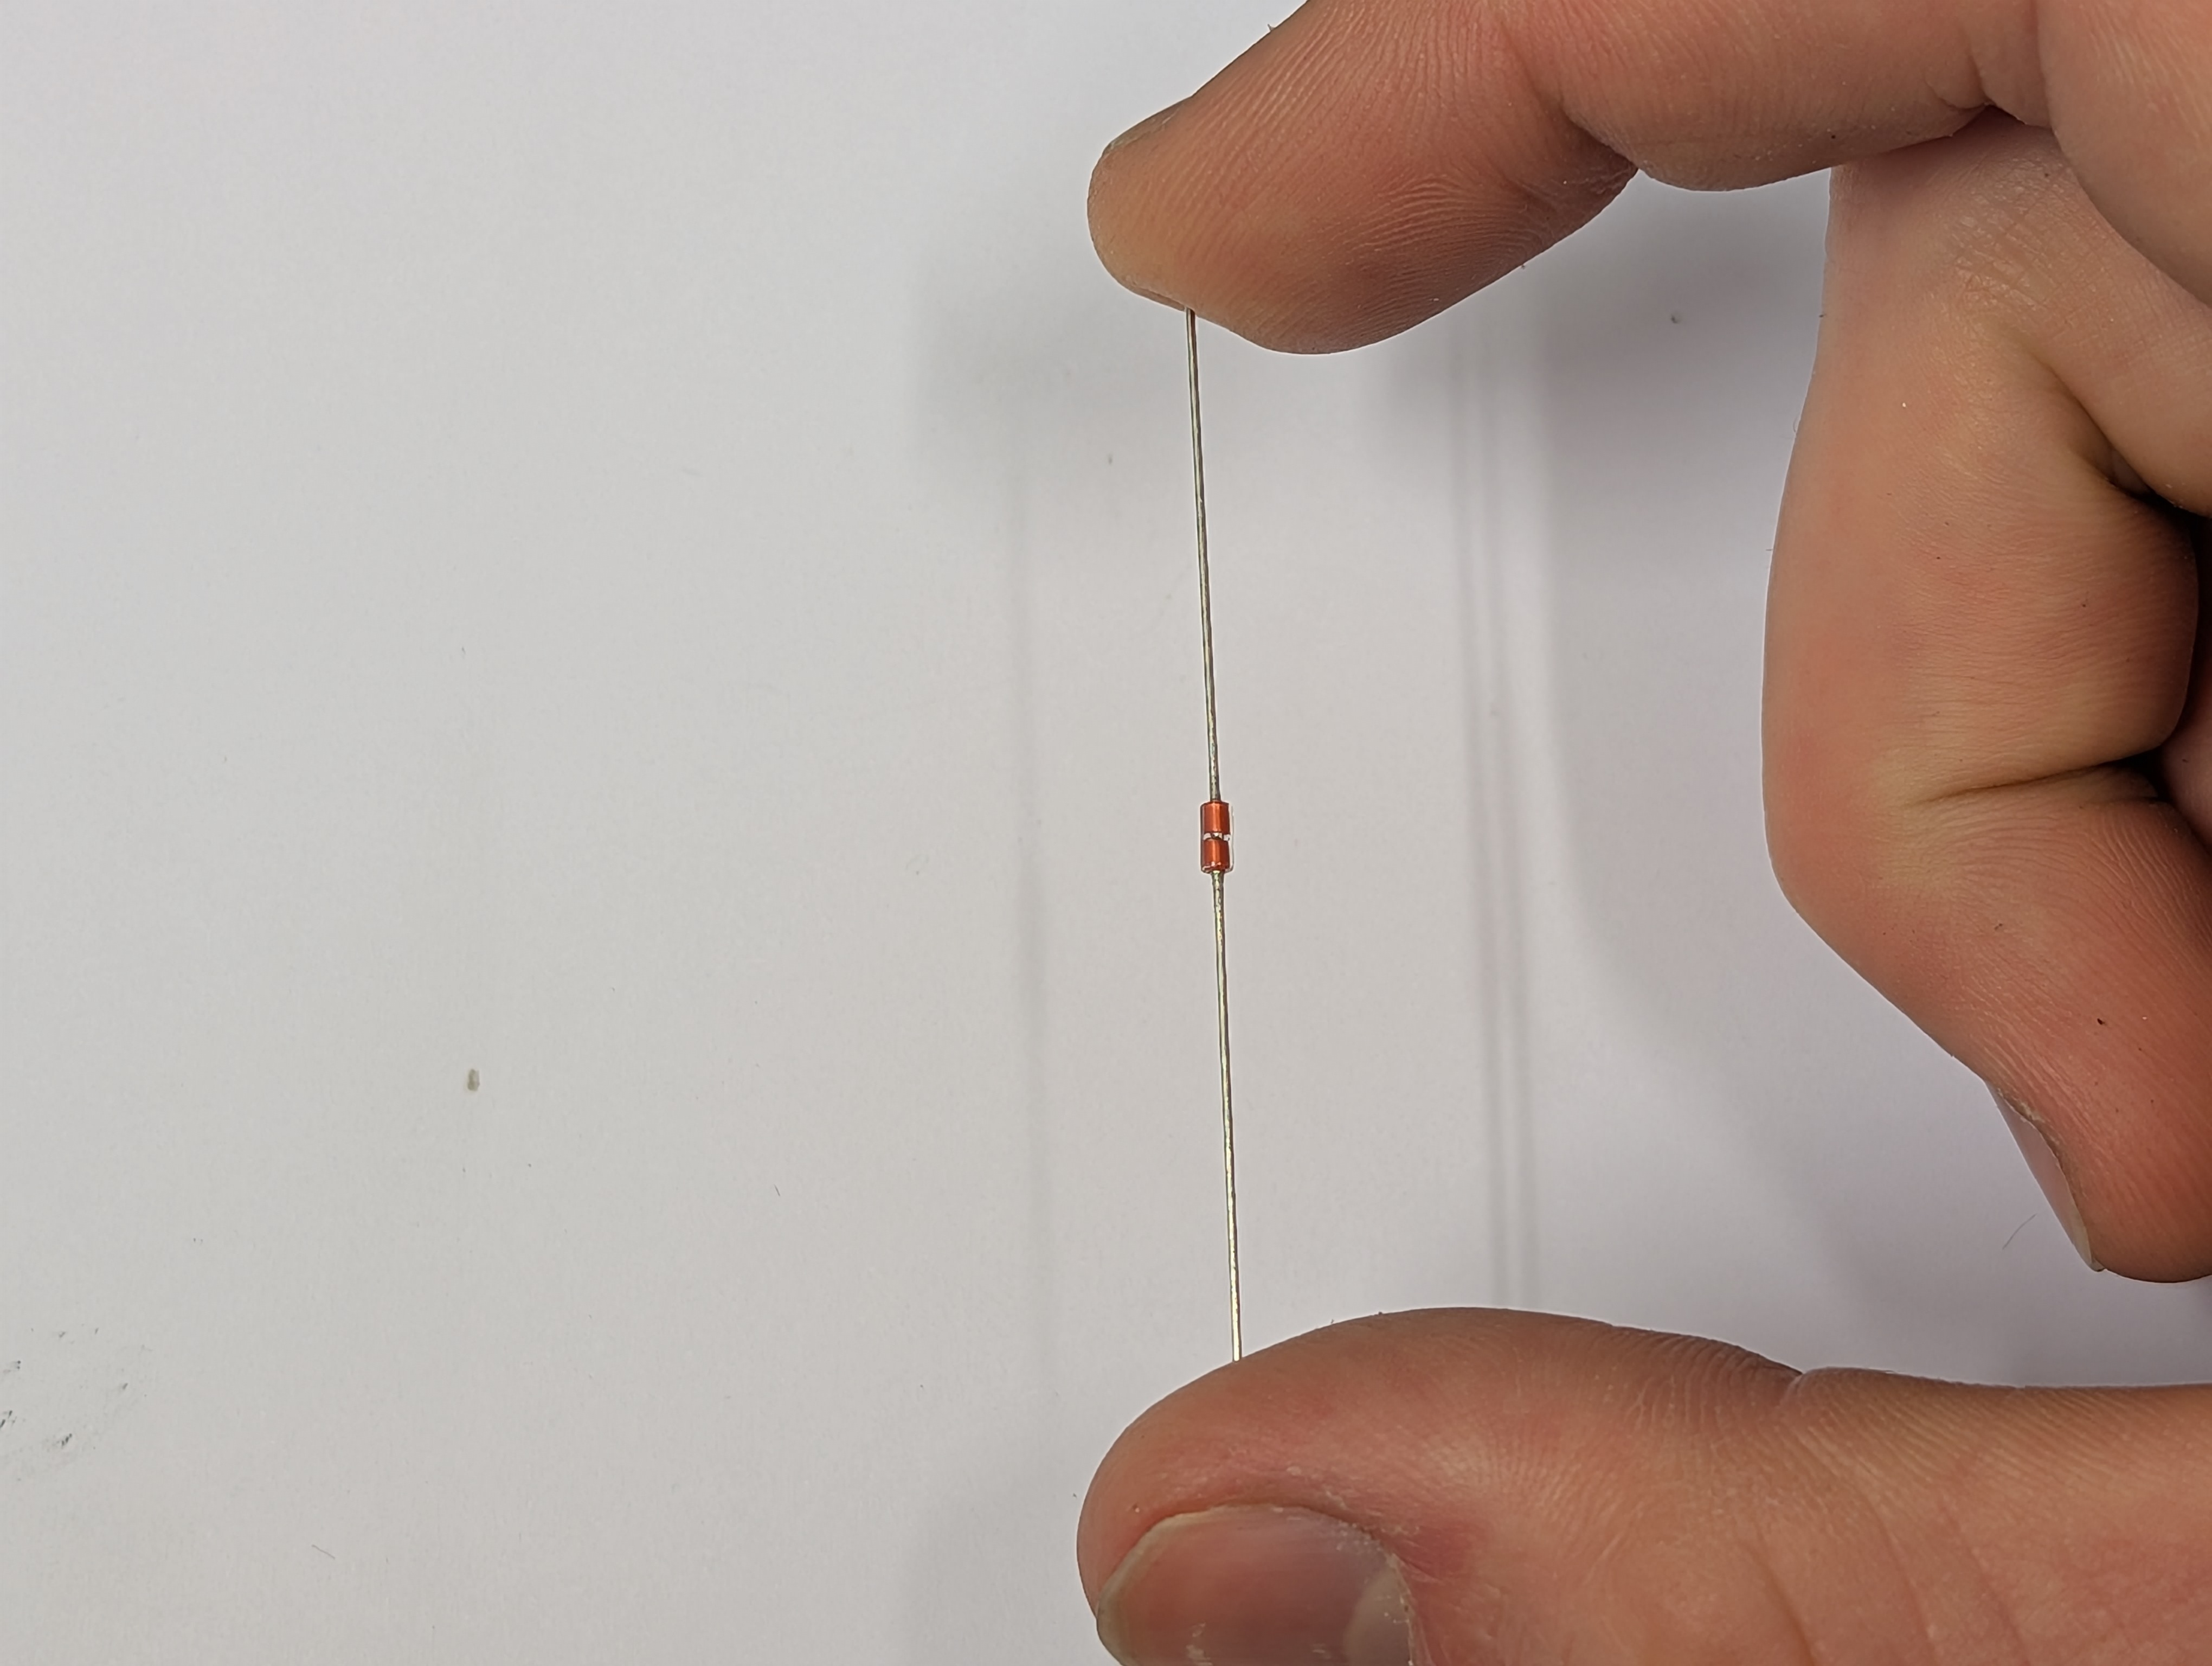
\includegraphics[width=0.75\textwidth]{pictures_of_construction/instruction_step_18.jpg}
\end{figure}

\begin{figure}[H]
    \centering
    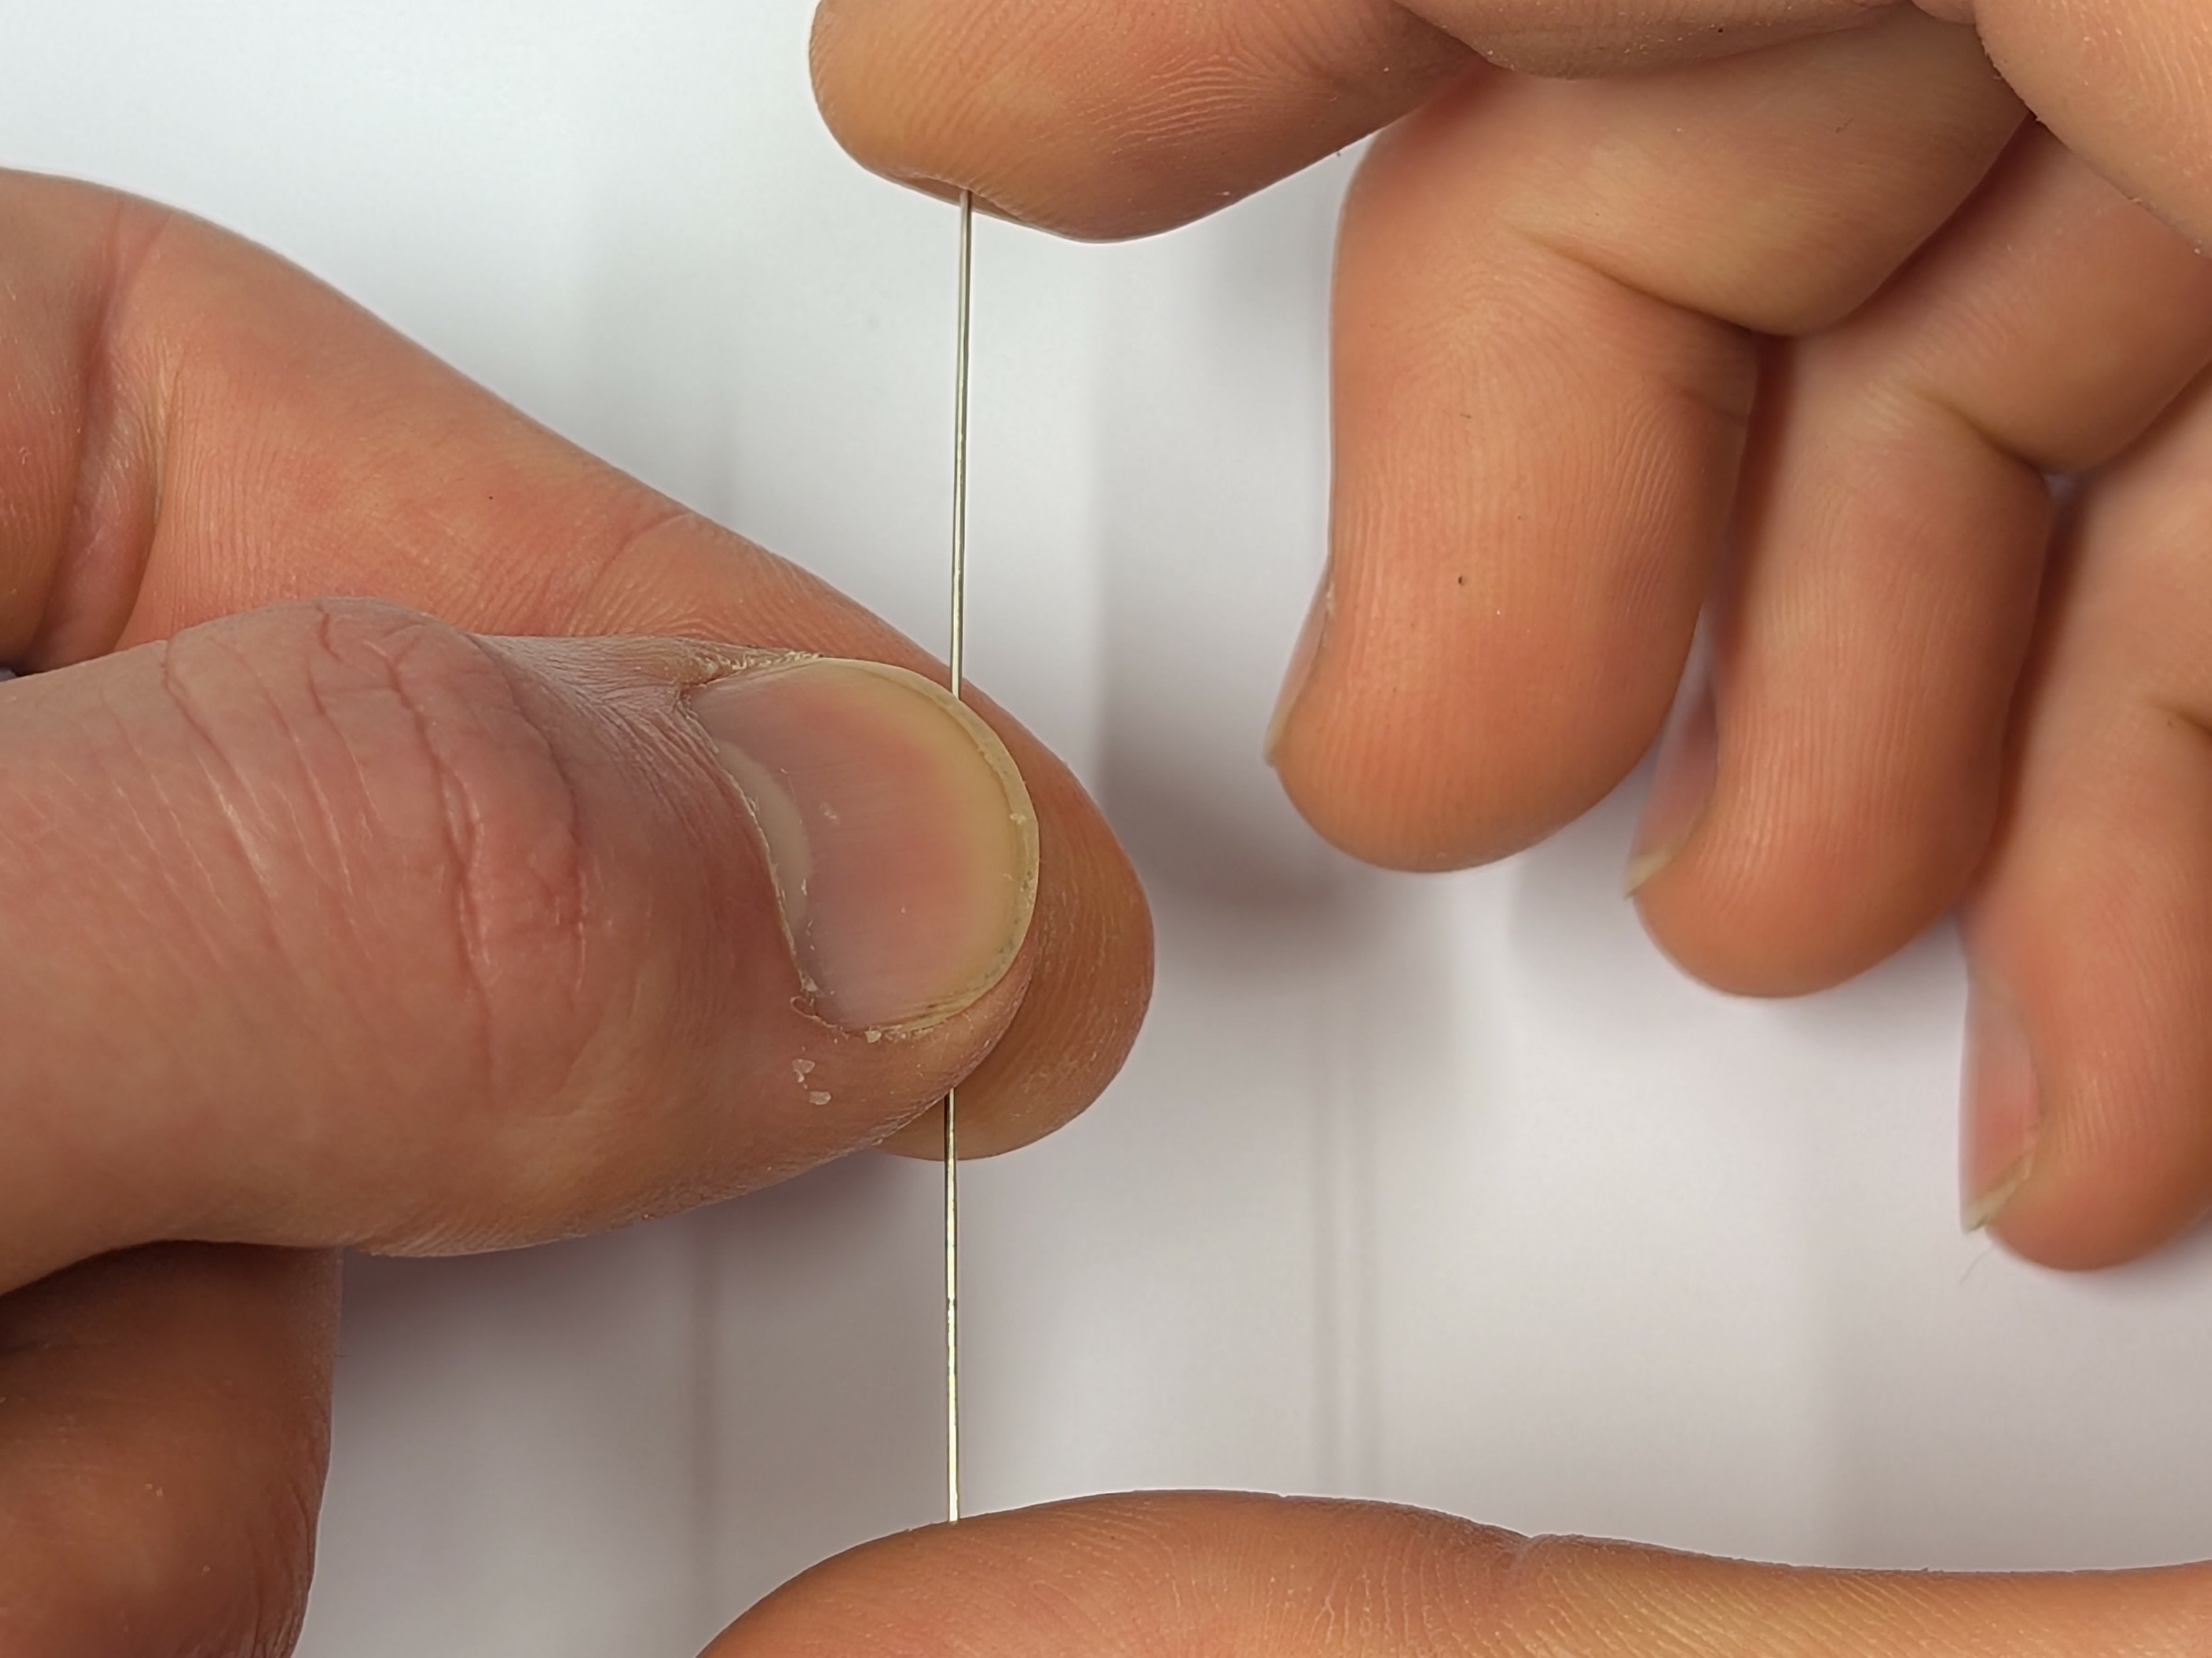
\includegraphics[width=0.75\textwidth]{pictures_of_construction/instruction_step_19.jpg}
\end{figure}

\begin{figure}[H]
    \centering
    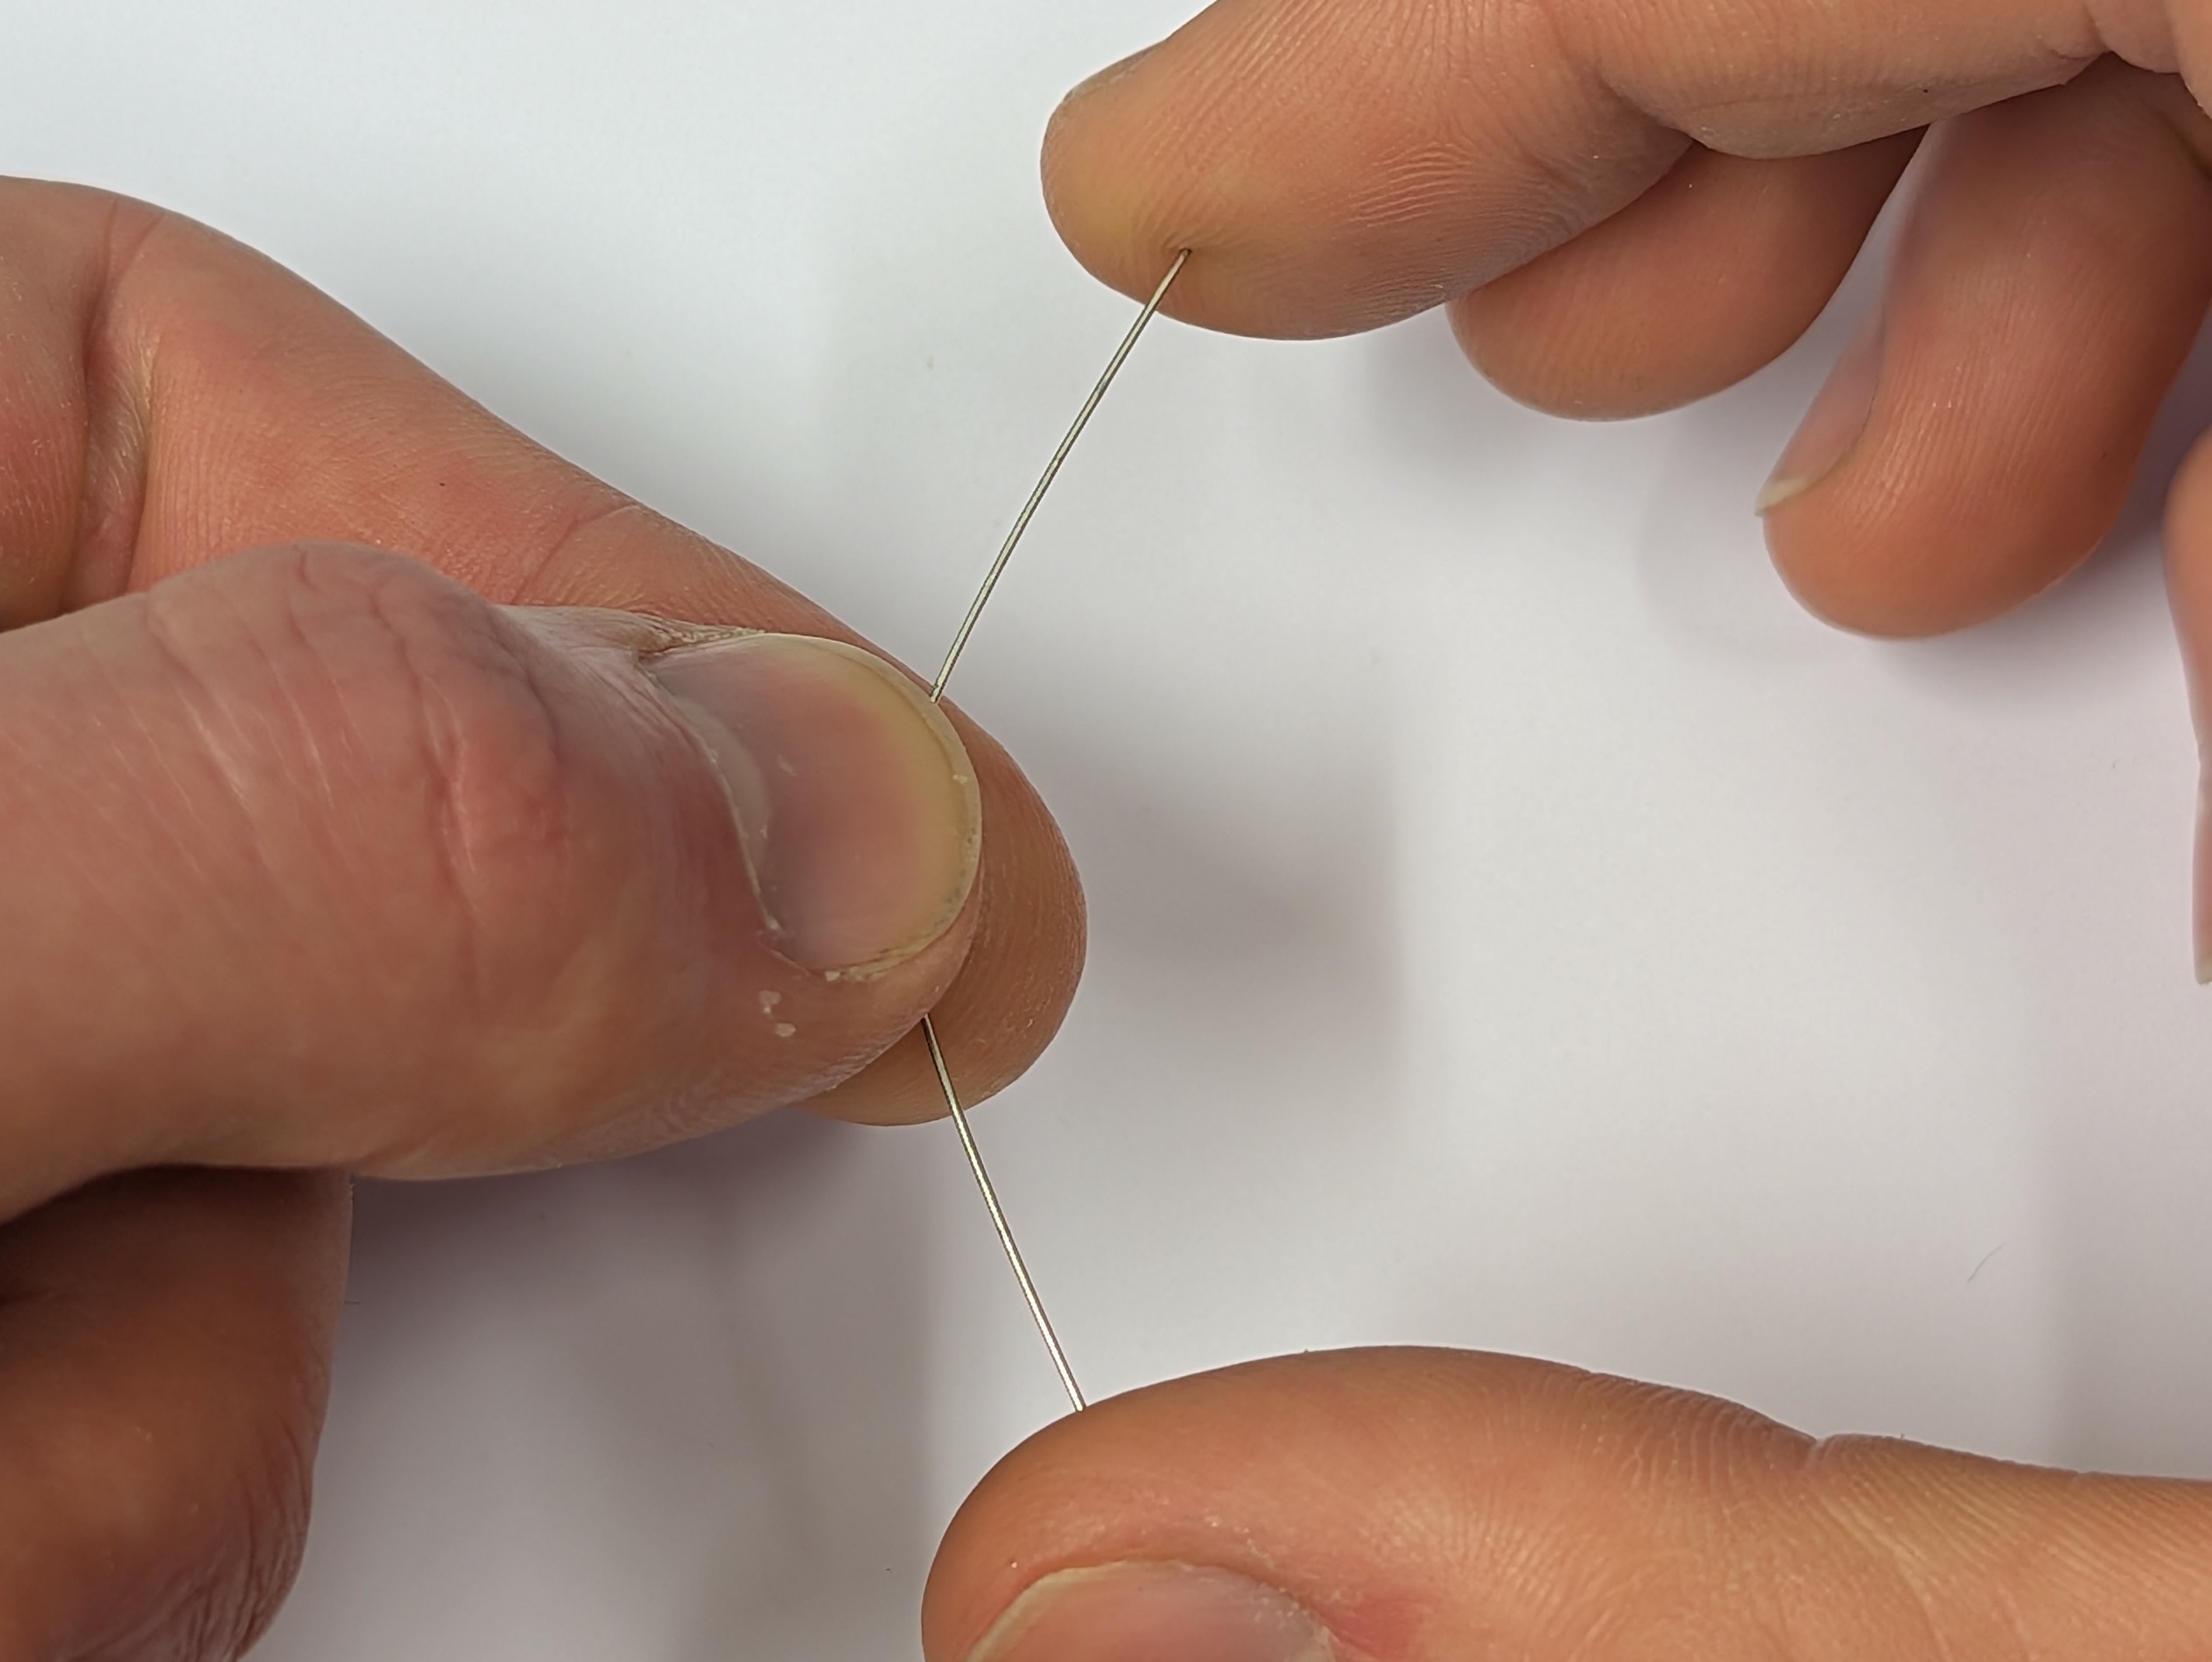
\includegraphics[width=0.75\textwidth]{pictures_of_construction/instruction_step_20.jpg}
\end{figure}

\begin{figure}[H]
    \centering
    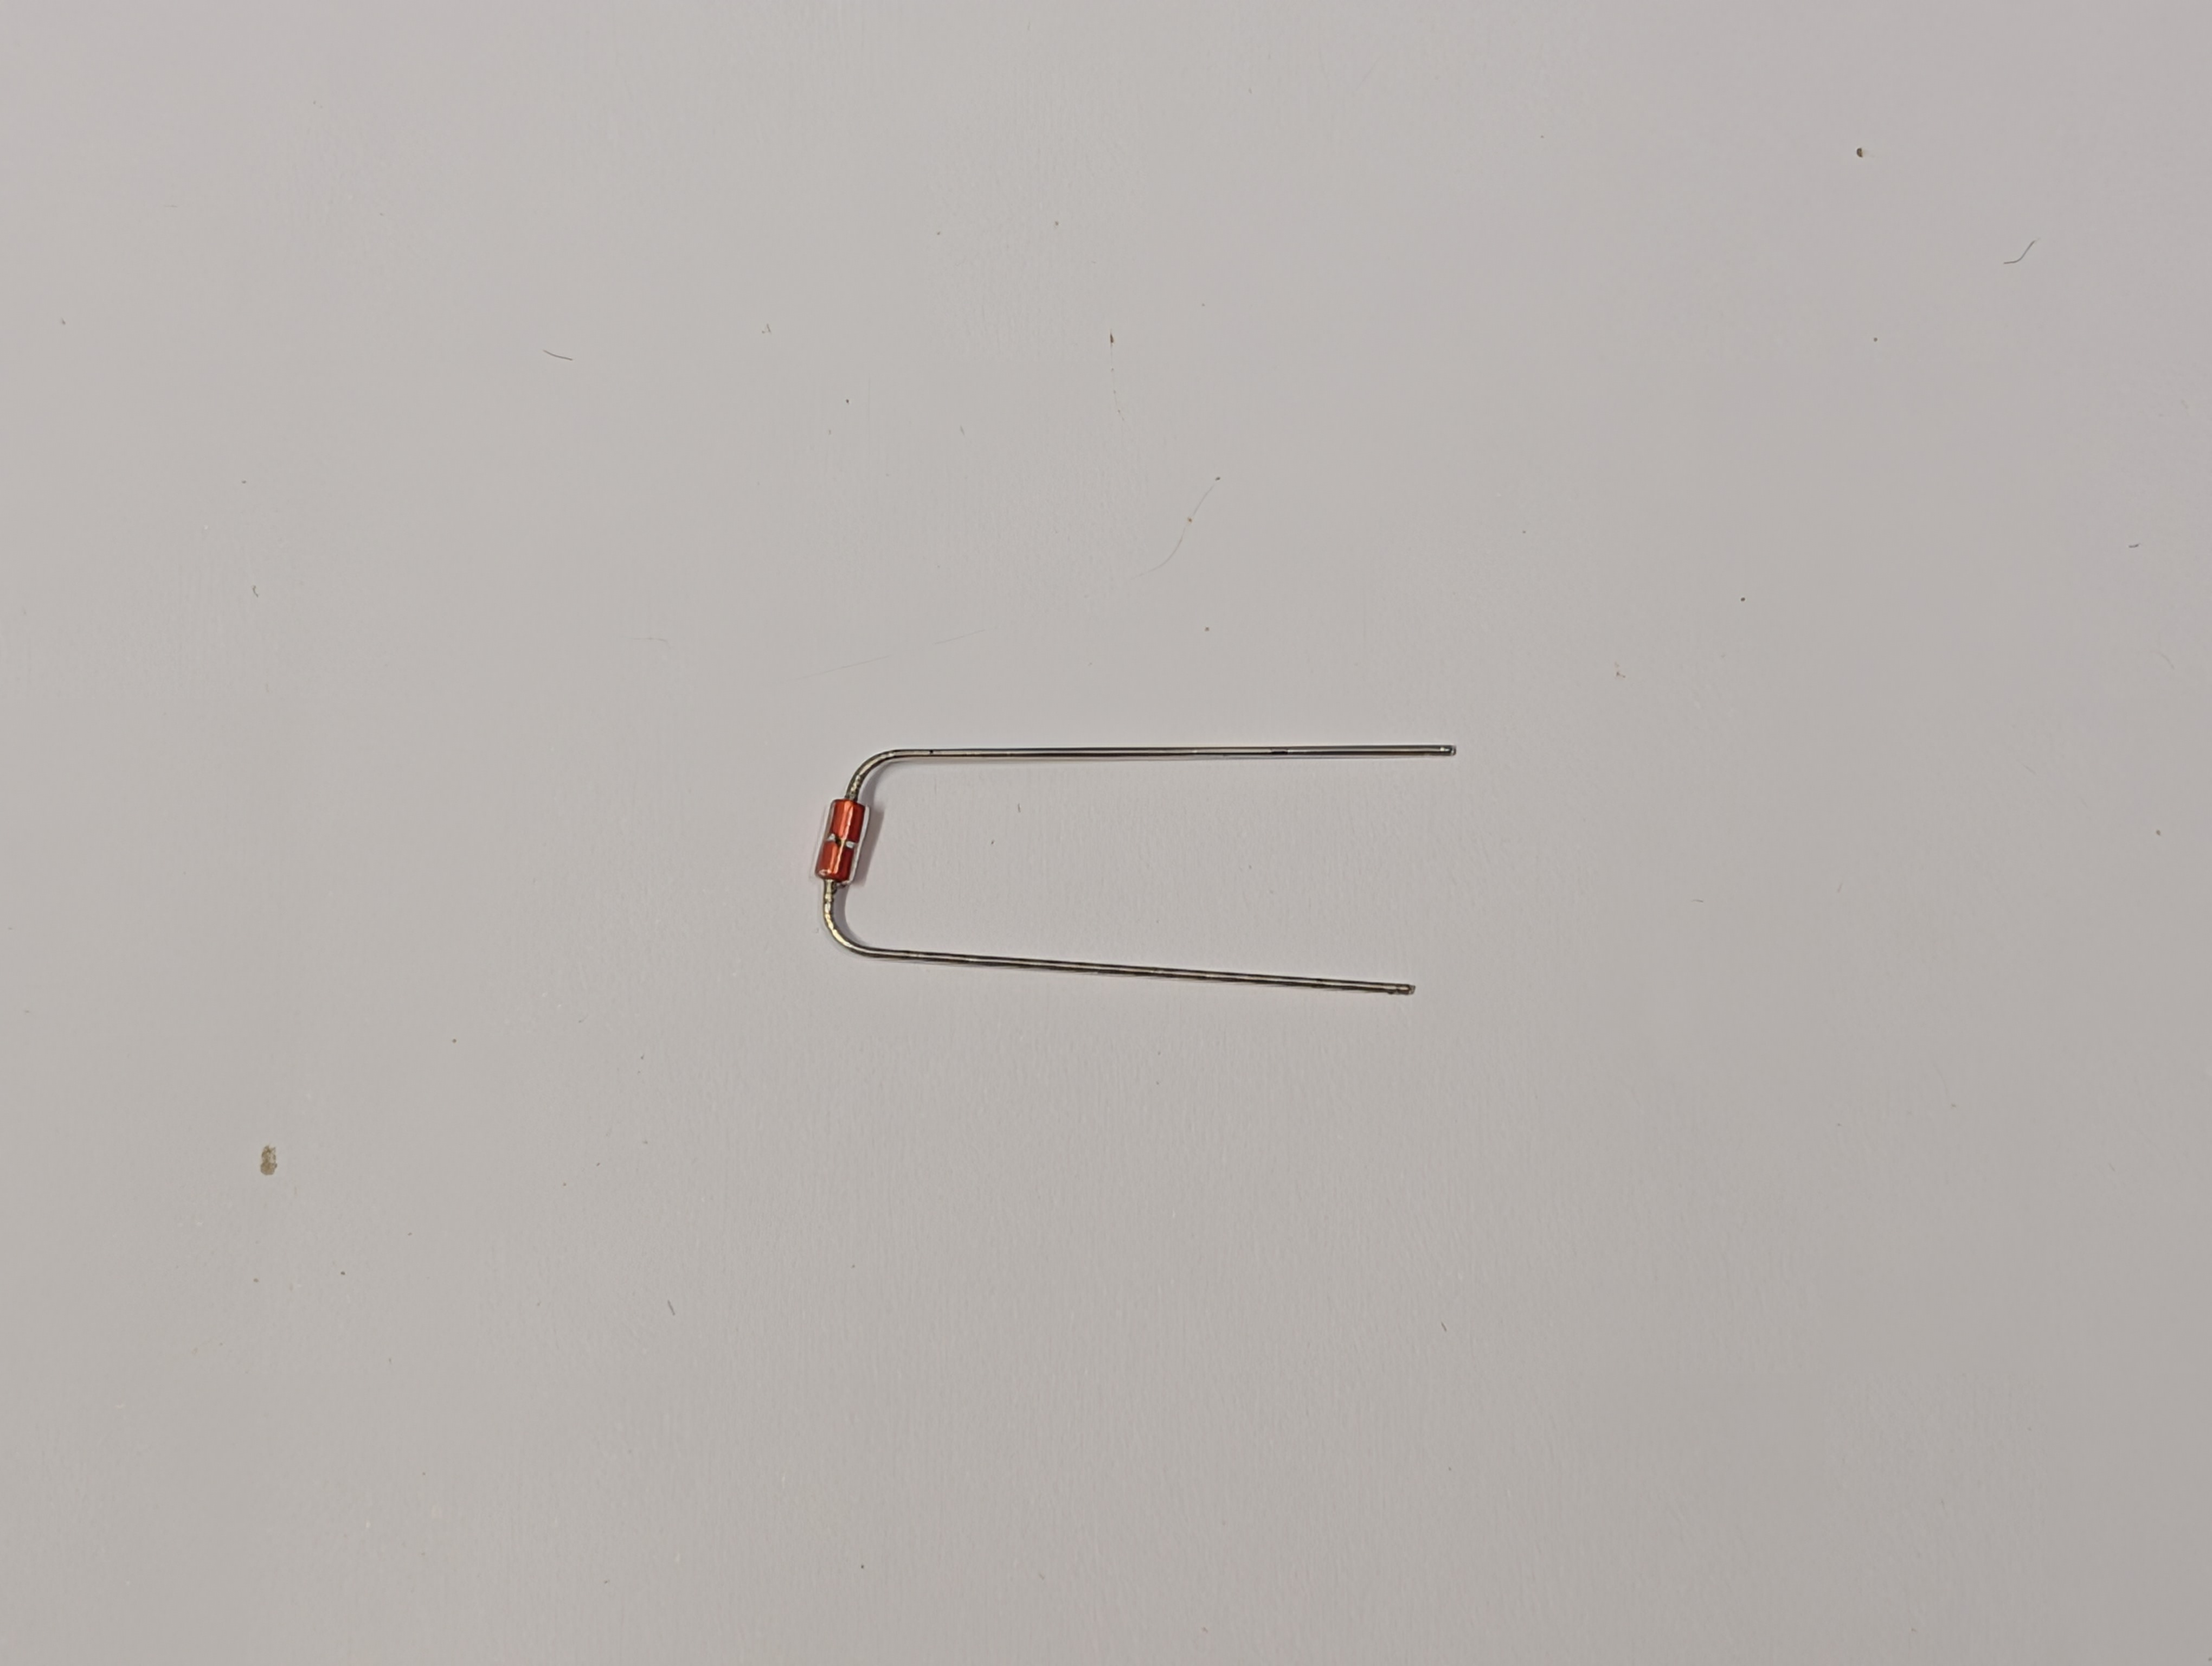
\includegraphics[width=0.75\textwidth]{pictures_of_construction/instruction_step_21.jpg}
\end{figure}

\begin{figure}[H]
    \centering
    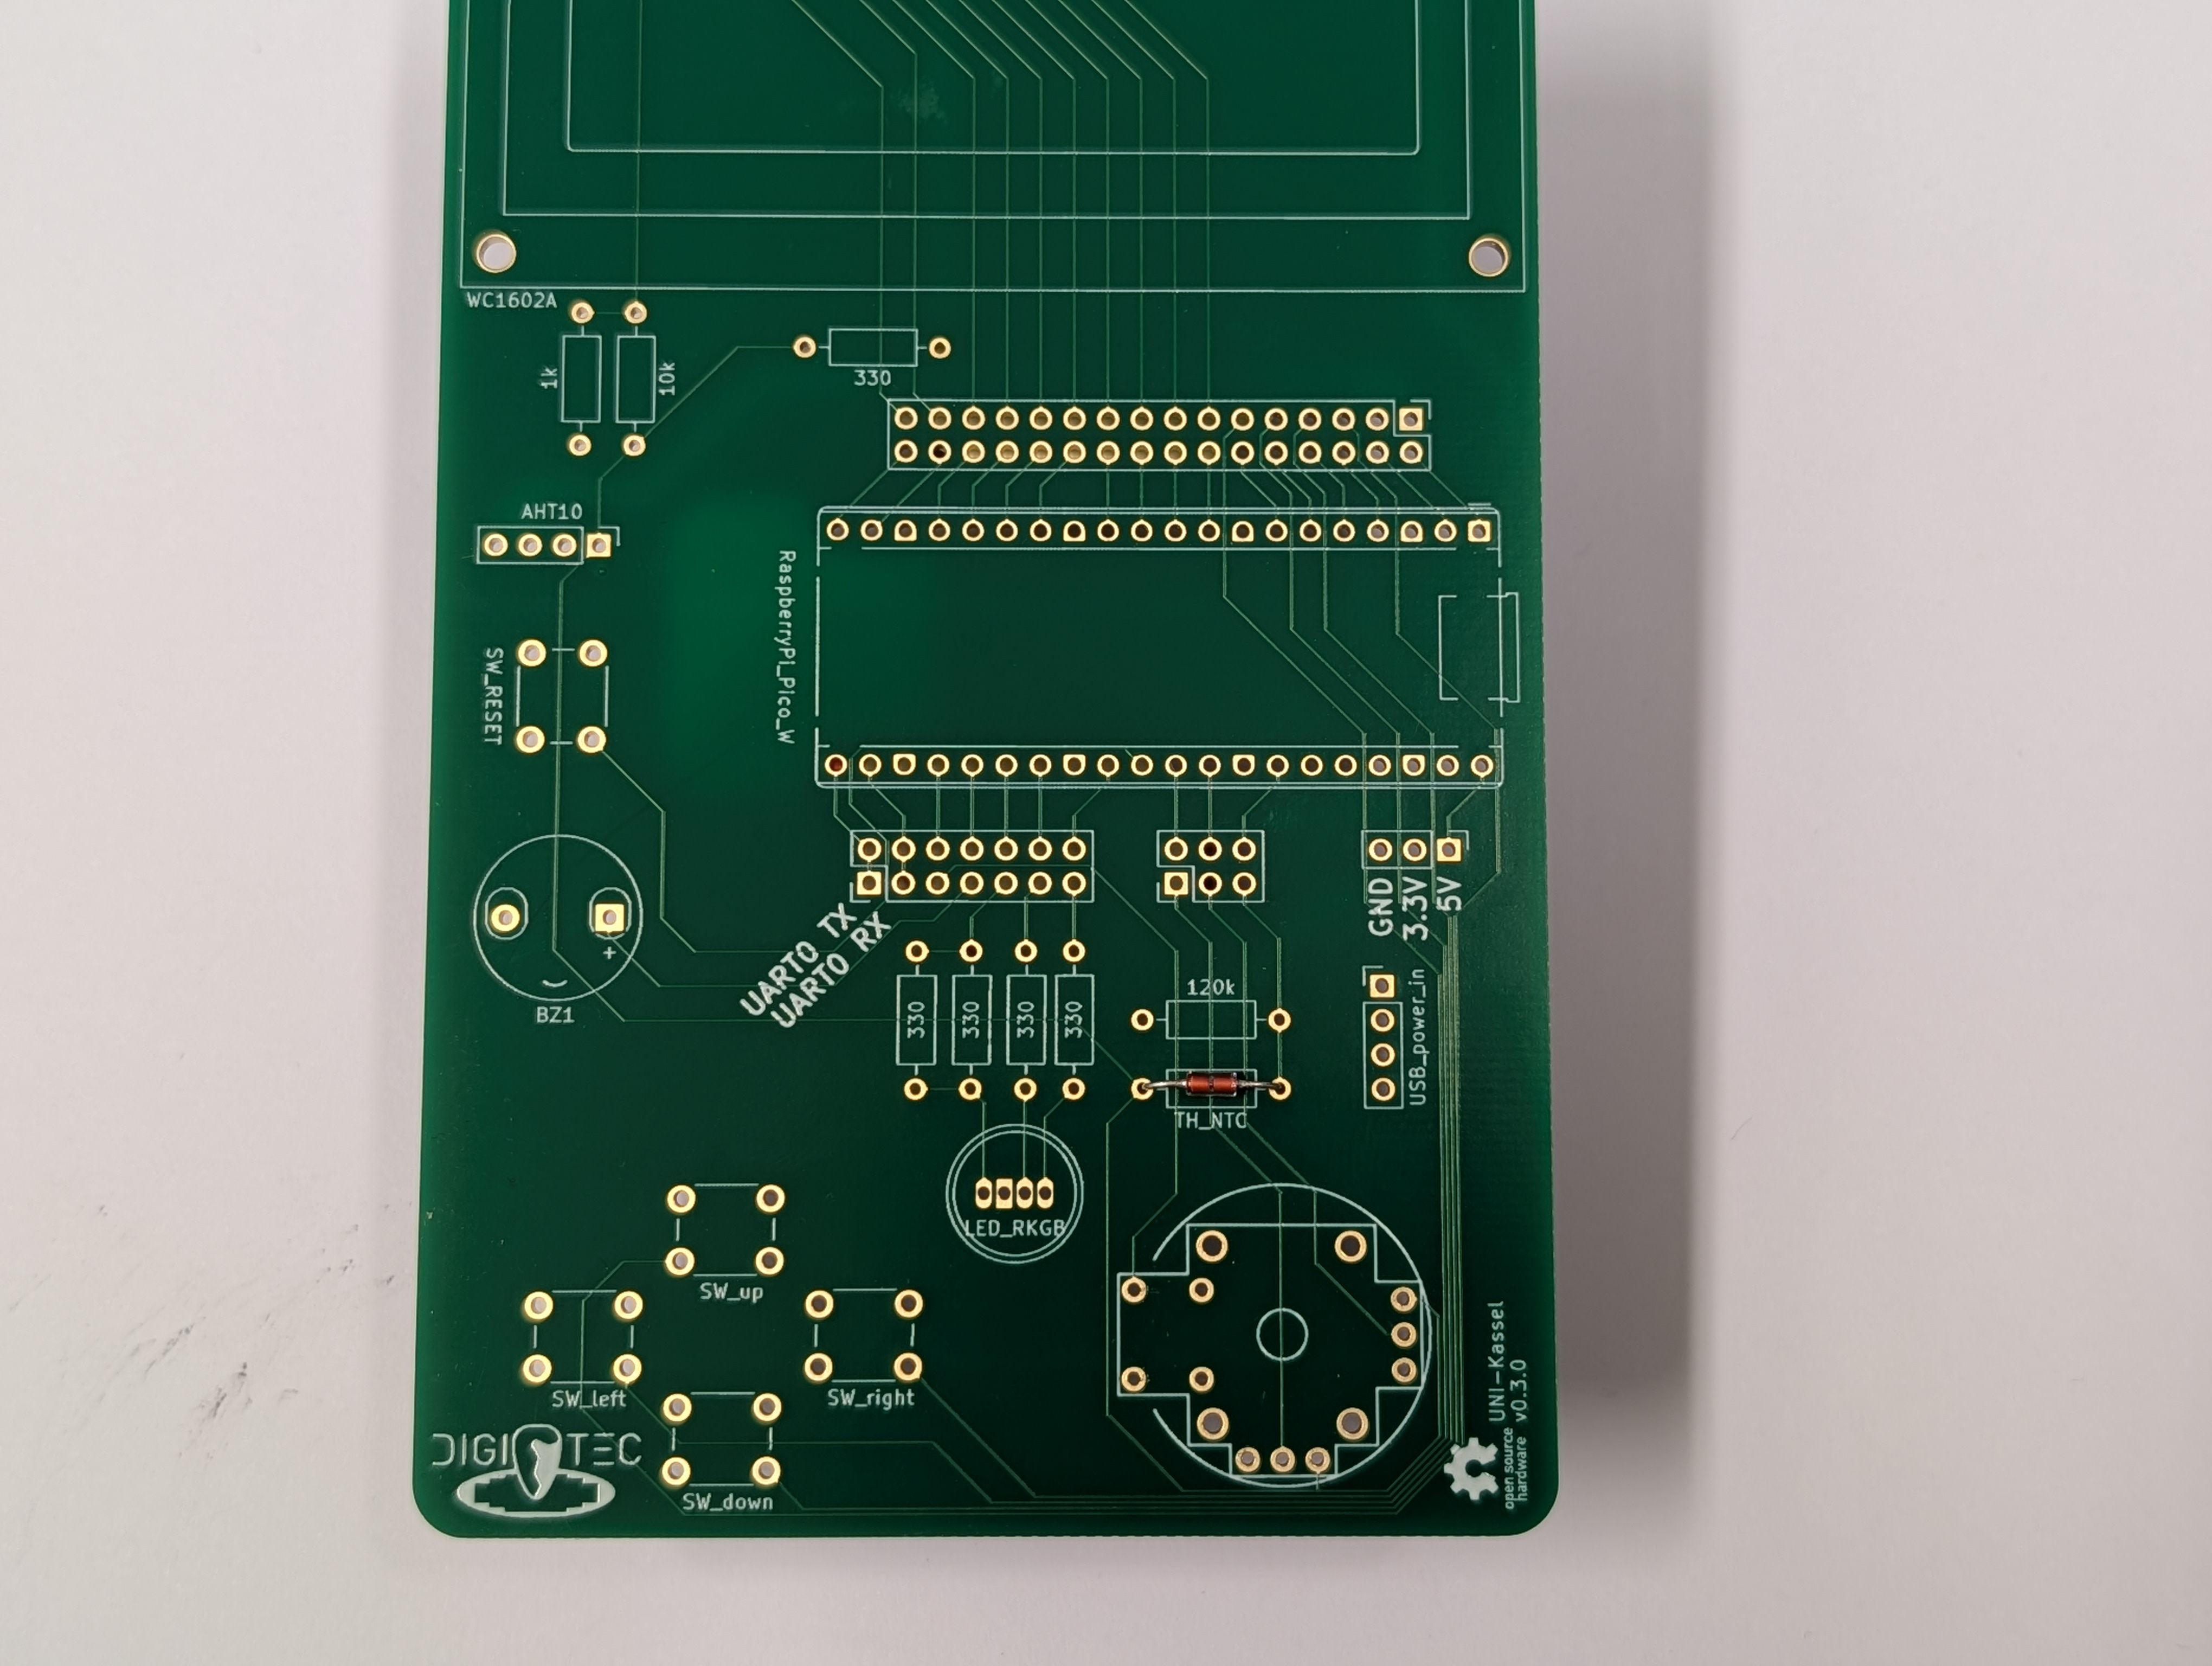
\includegraphics[width=0.75\textwidth]{pictures_of_construction/instruction_step_22.jpg}
\end{figure}

The newly formed resistor can now be inserted into the Buzzerino PCB at the position marked \texttt{TH\_NTC}.\\
\textbf{Important:} The printed side of the Buzzerino PCB is the front of the PCB. The lower left corner should have our DIGETEC logo.

\begin{figure}[H]
    \centering
    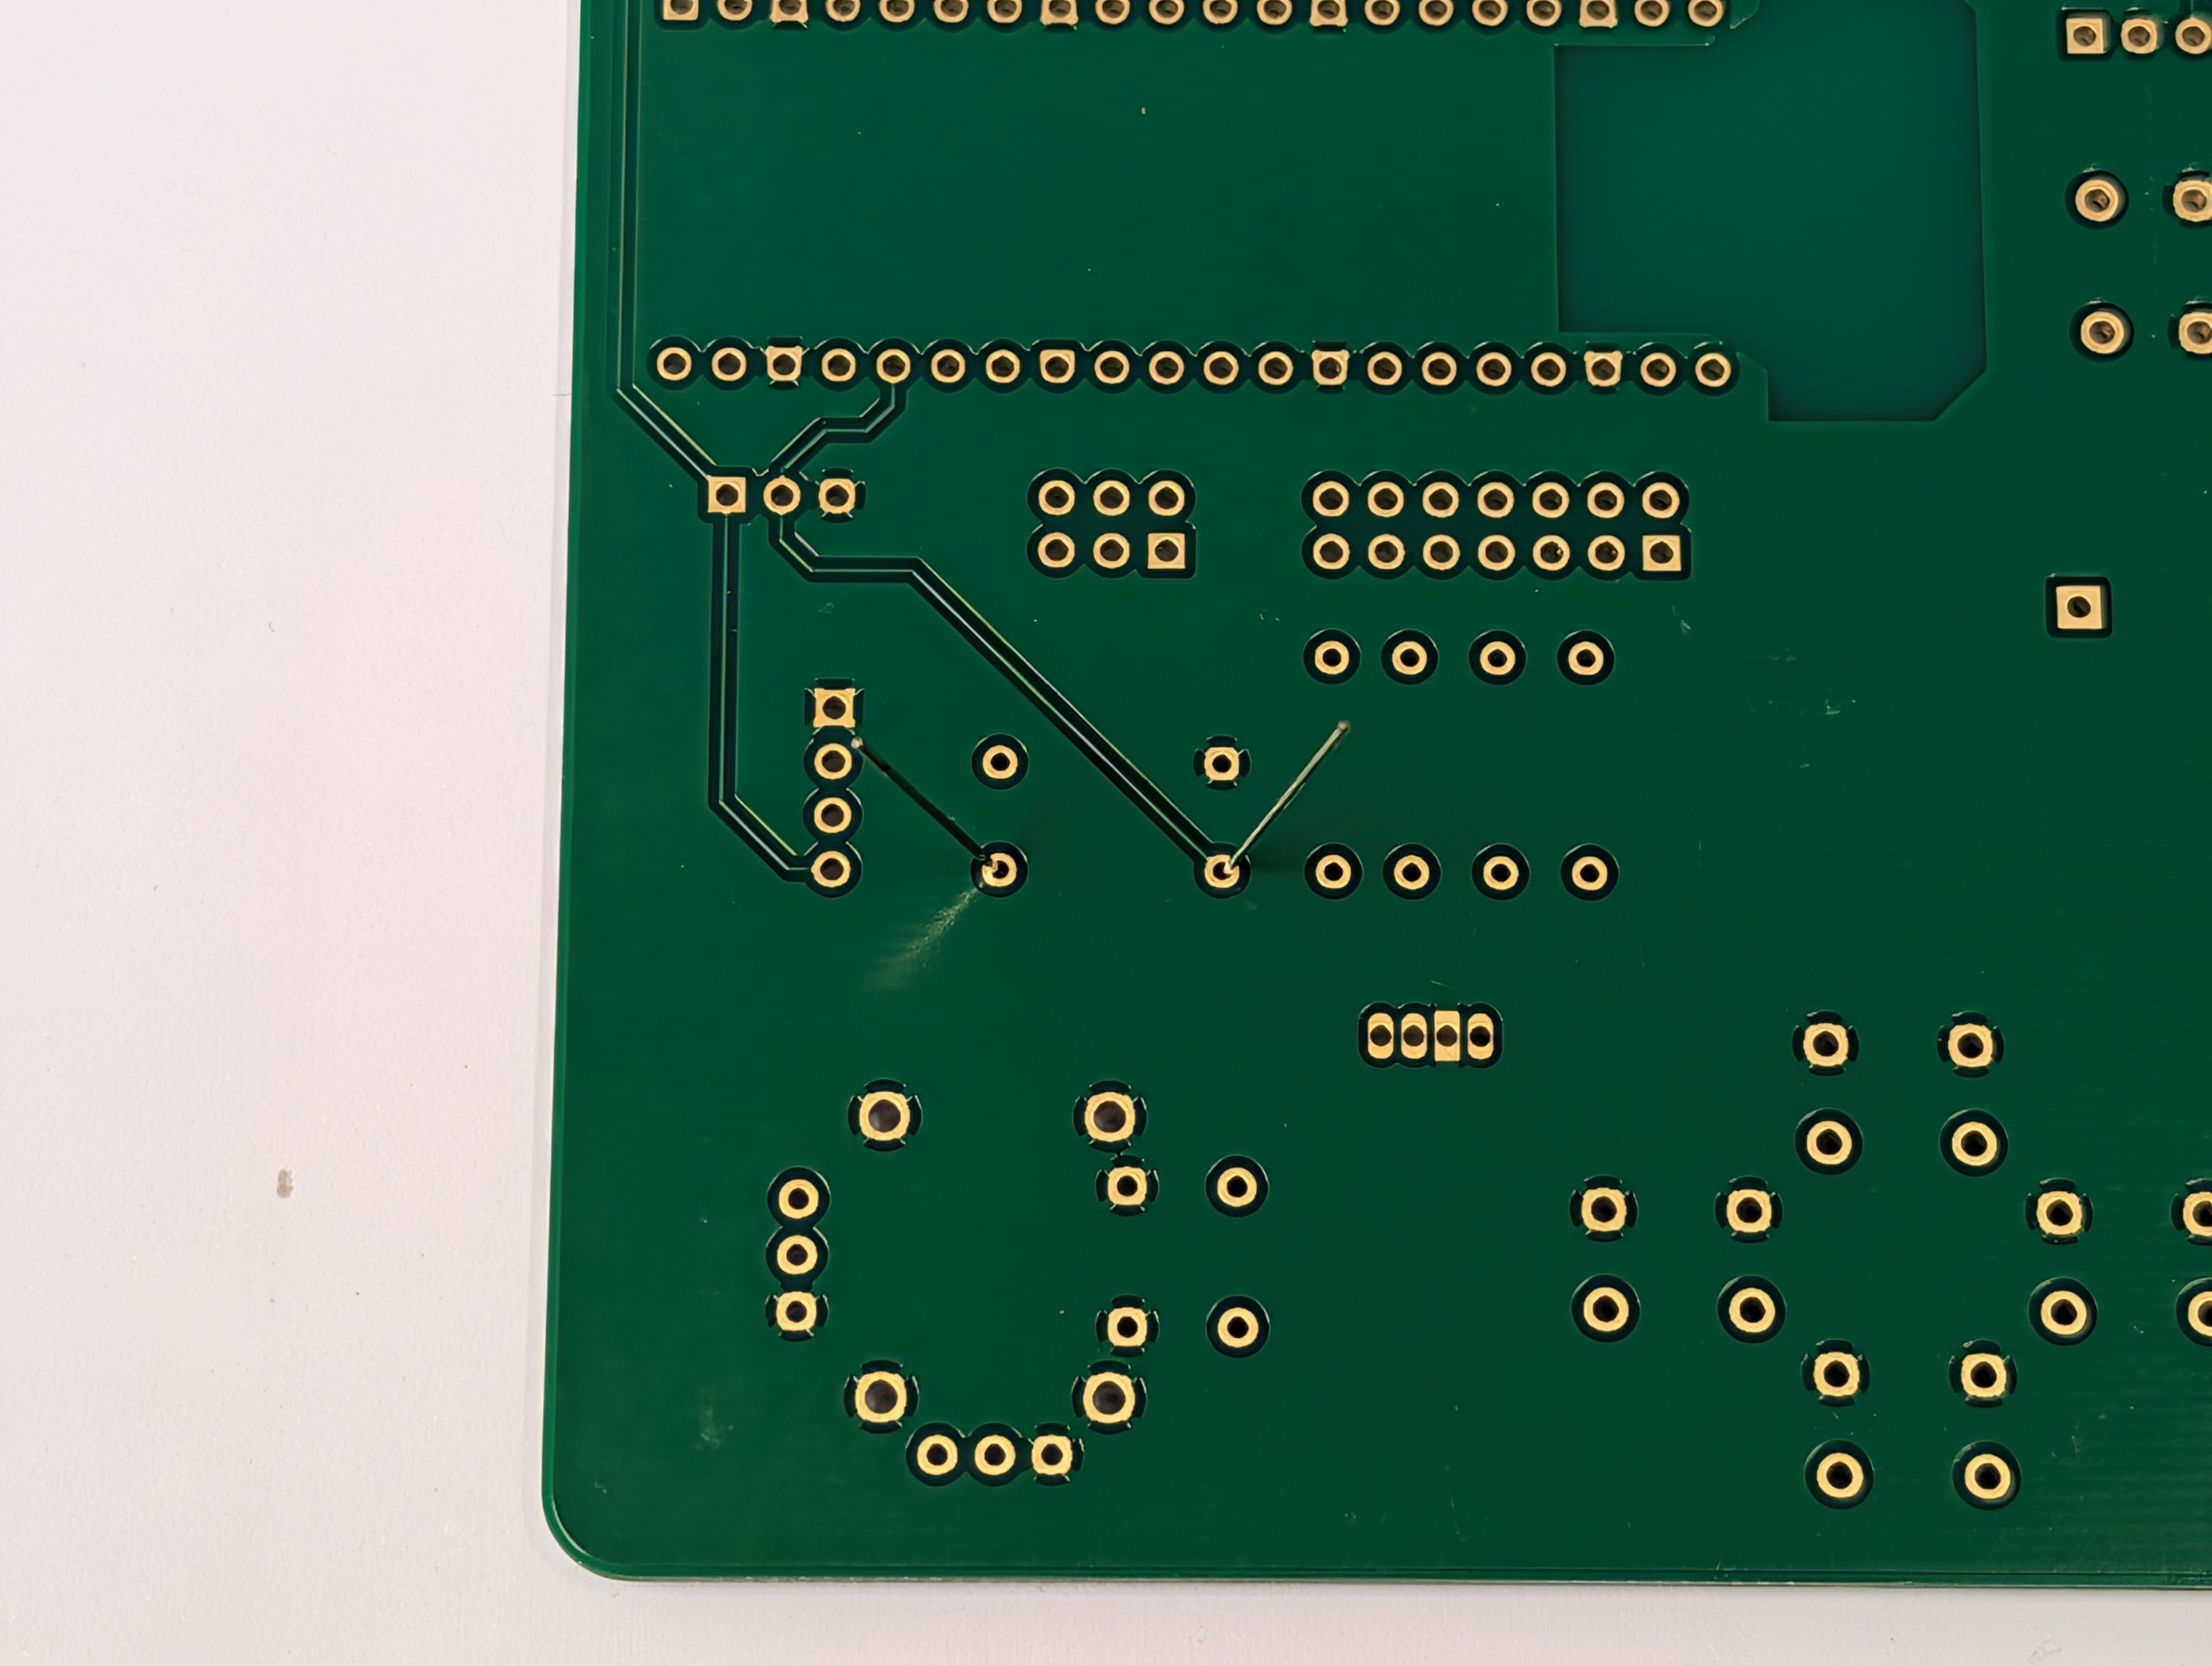
\includegraphics[width=0.75\textwidth]{pictures_of_construction/instruction_step_23.jpg}
\end{figure}

As a tip for soldering beginners, you can slightly bend the leads outwards after fully seating the resistor. This will help keep it in place.

\begin{figure}[H]
    \centering
    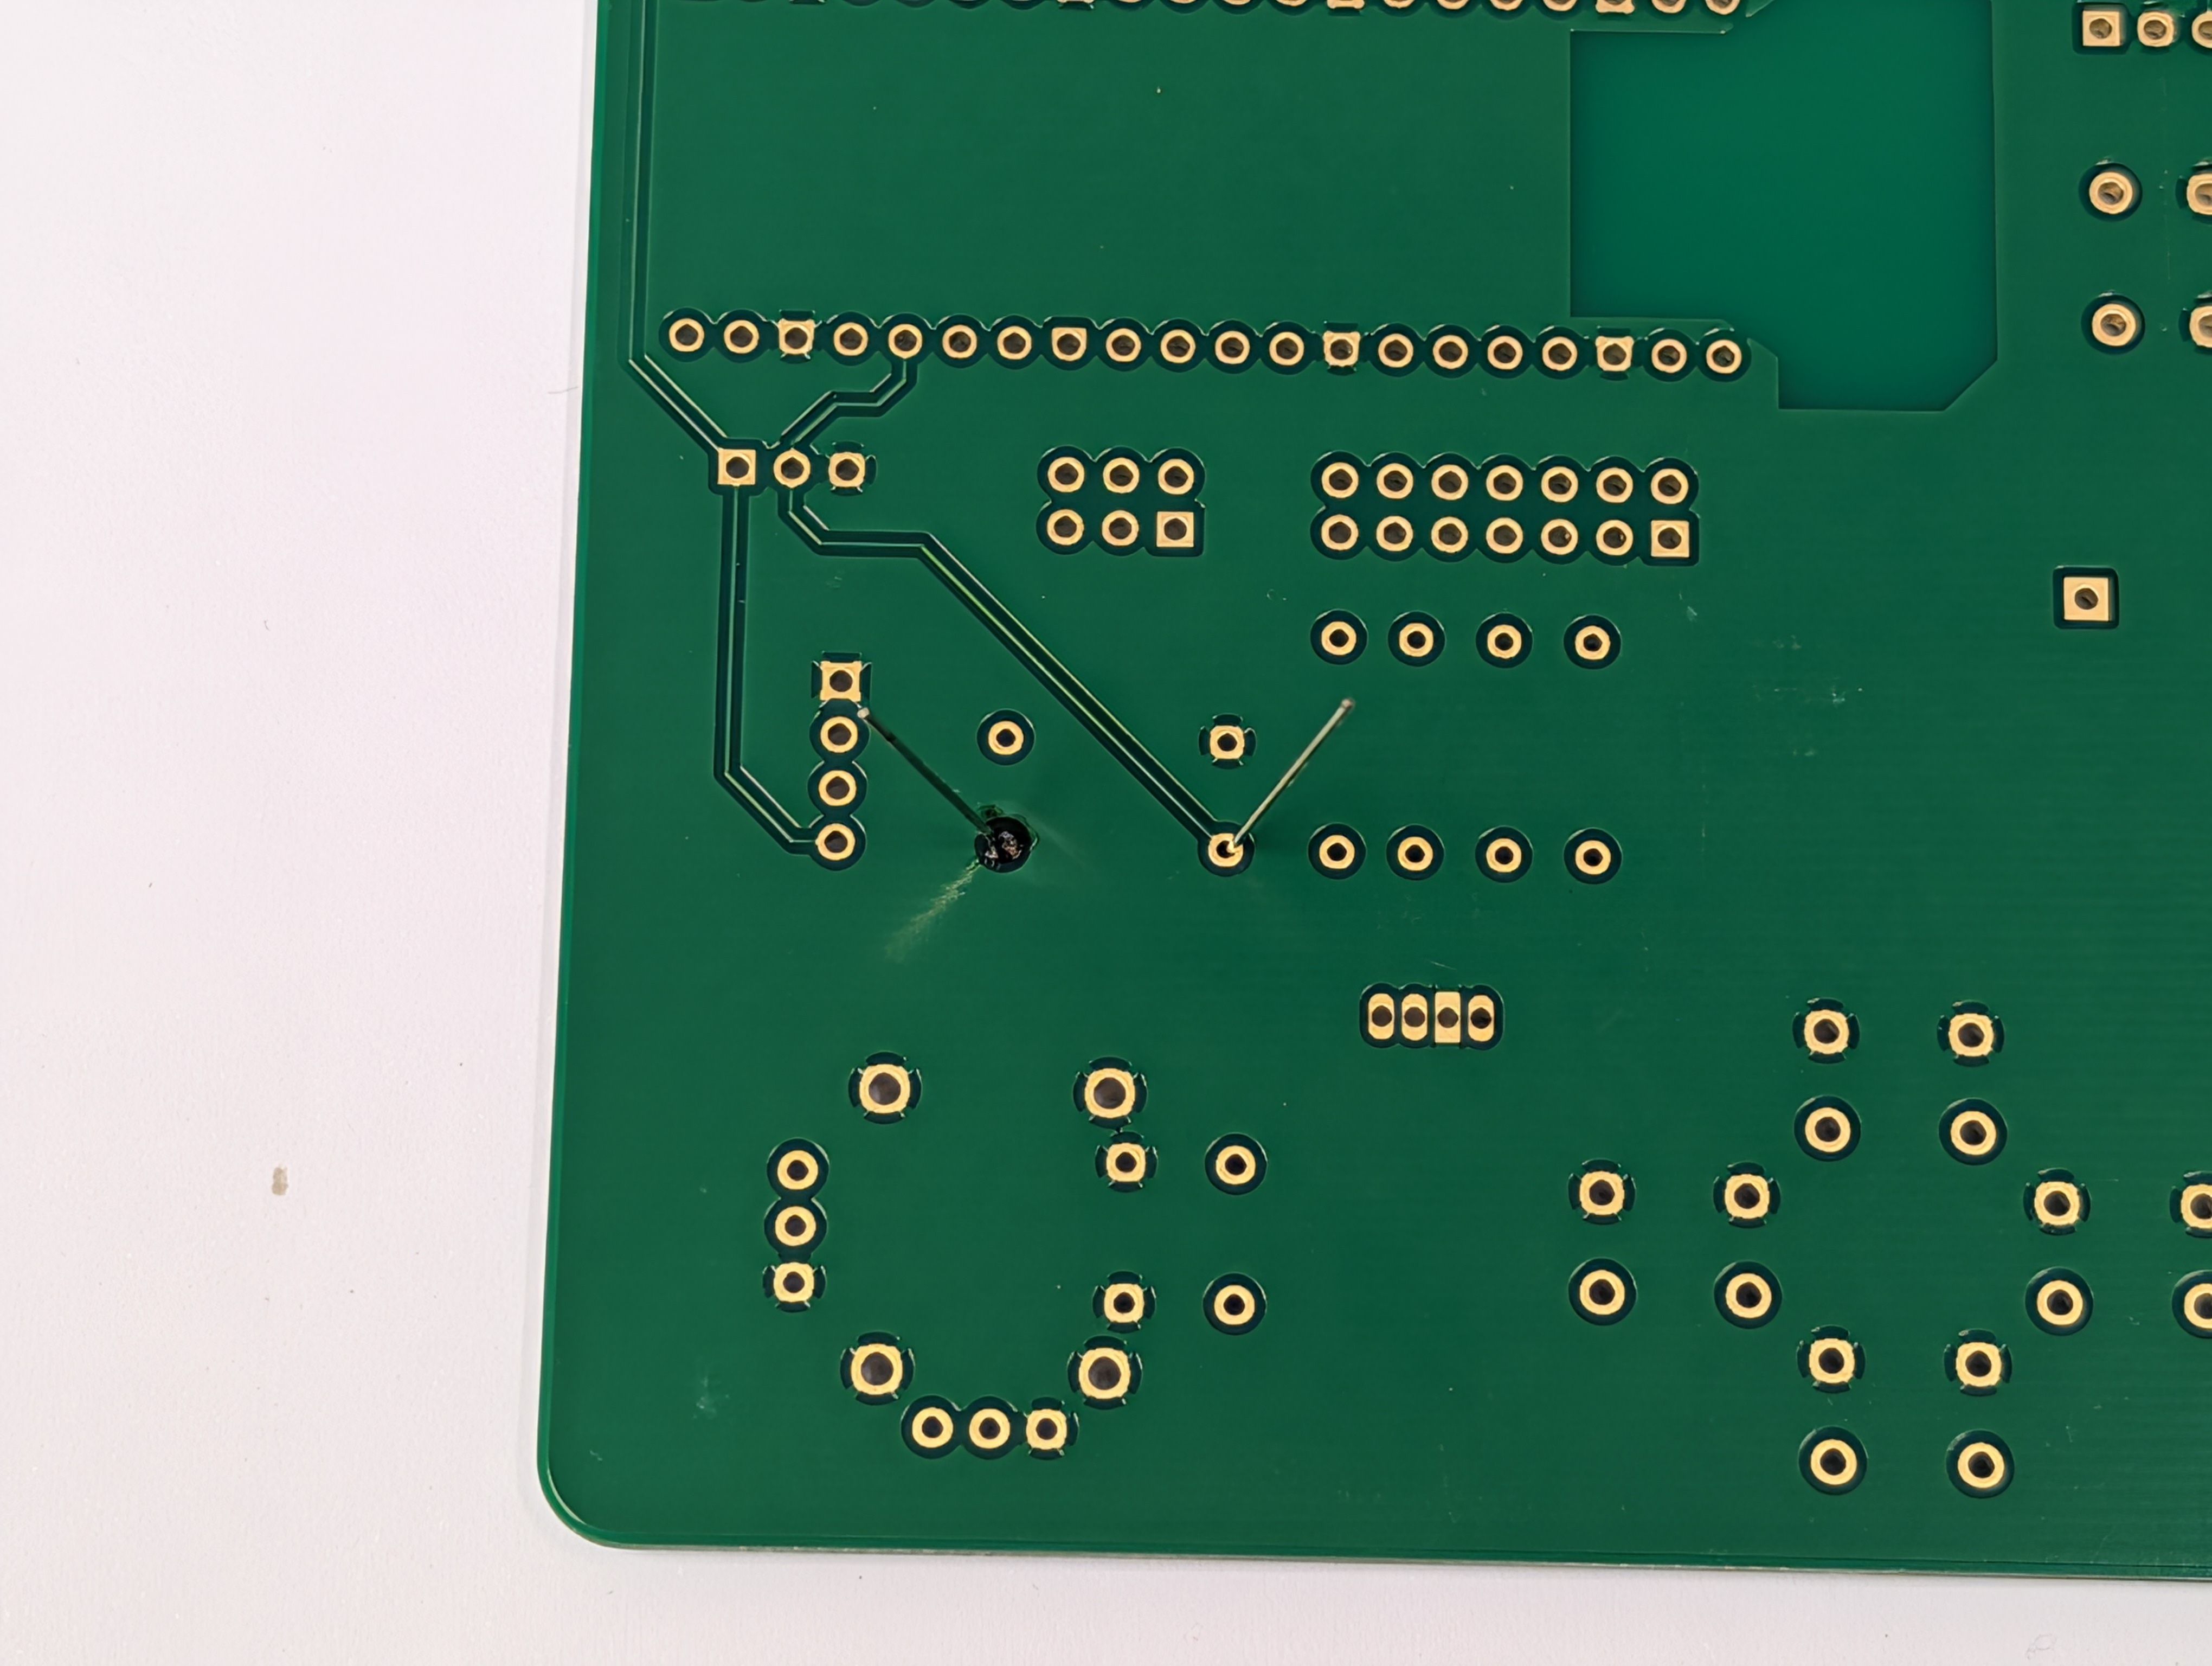
\includegraphics[width=0.75\textwidth]{pictures_of_construction/instruction_step_24.jpg}
\end{figure}

Like the previous solder joints, it is good practice to start by soldering one lead first, then correct the positioning, and finally solder both.

\begin{figure}[H]
    \centering
    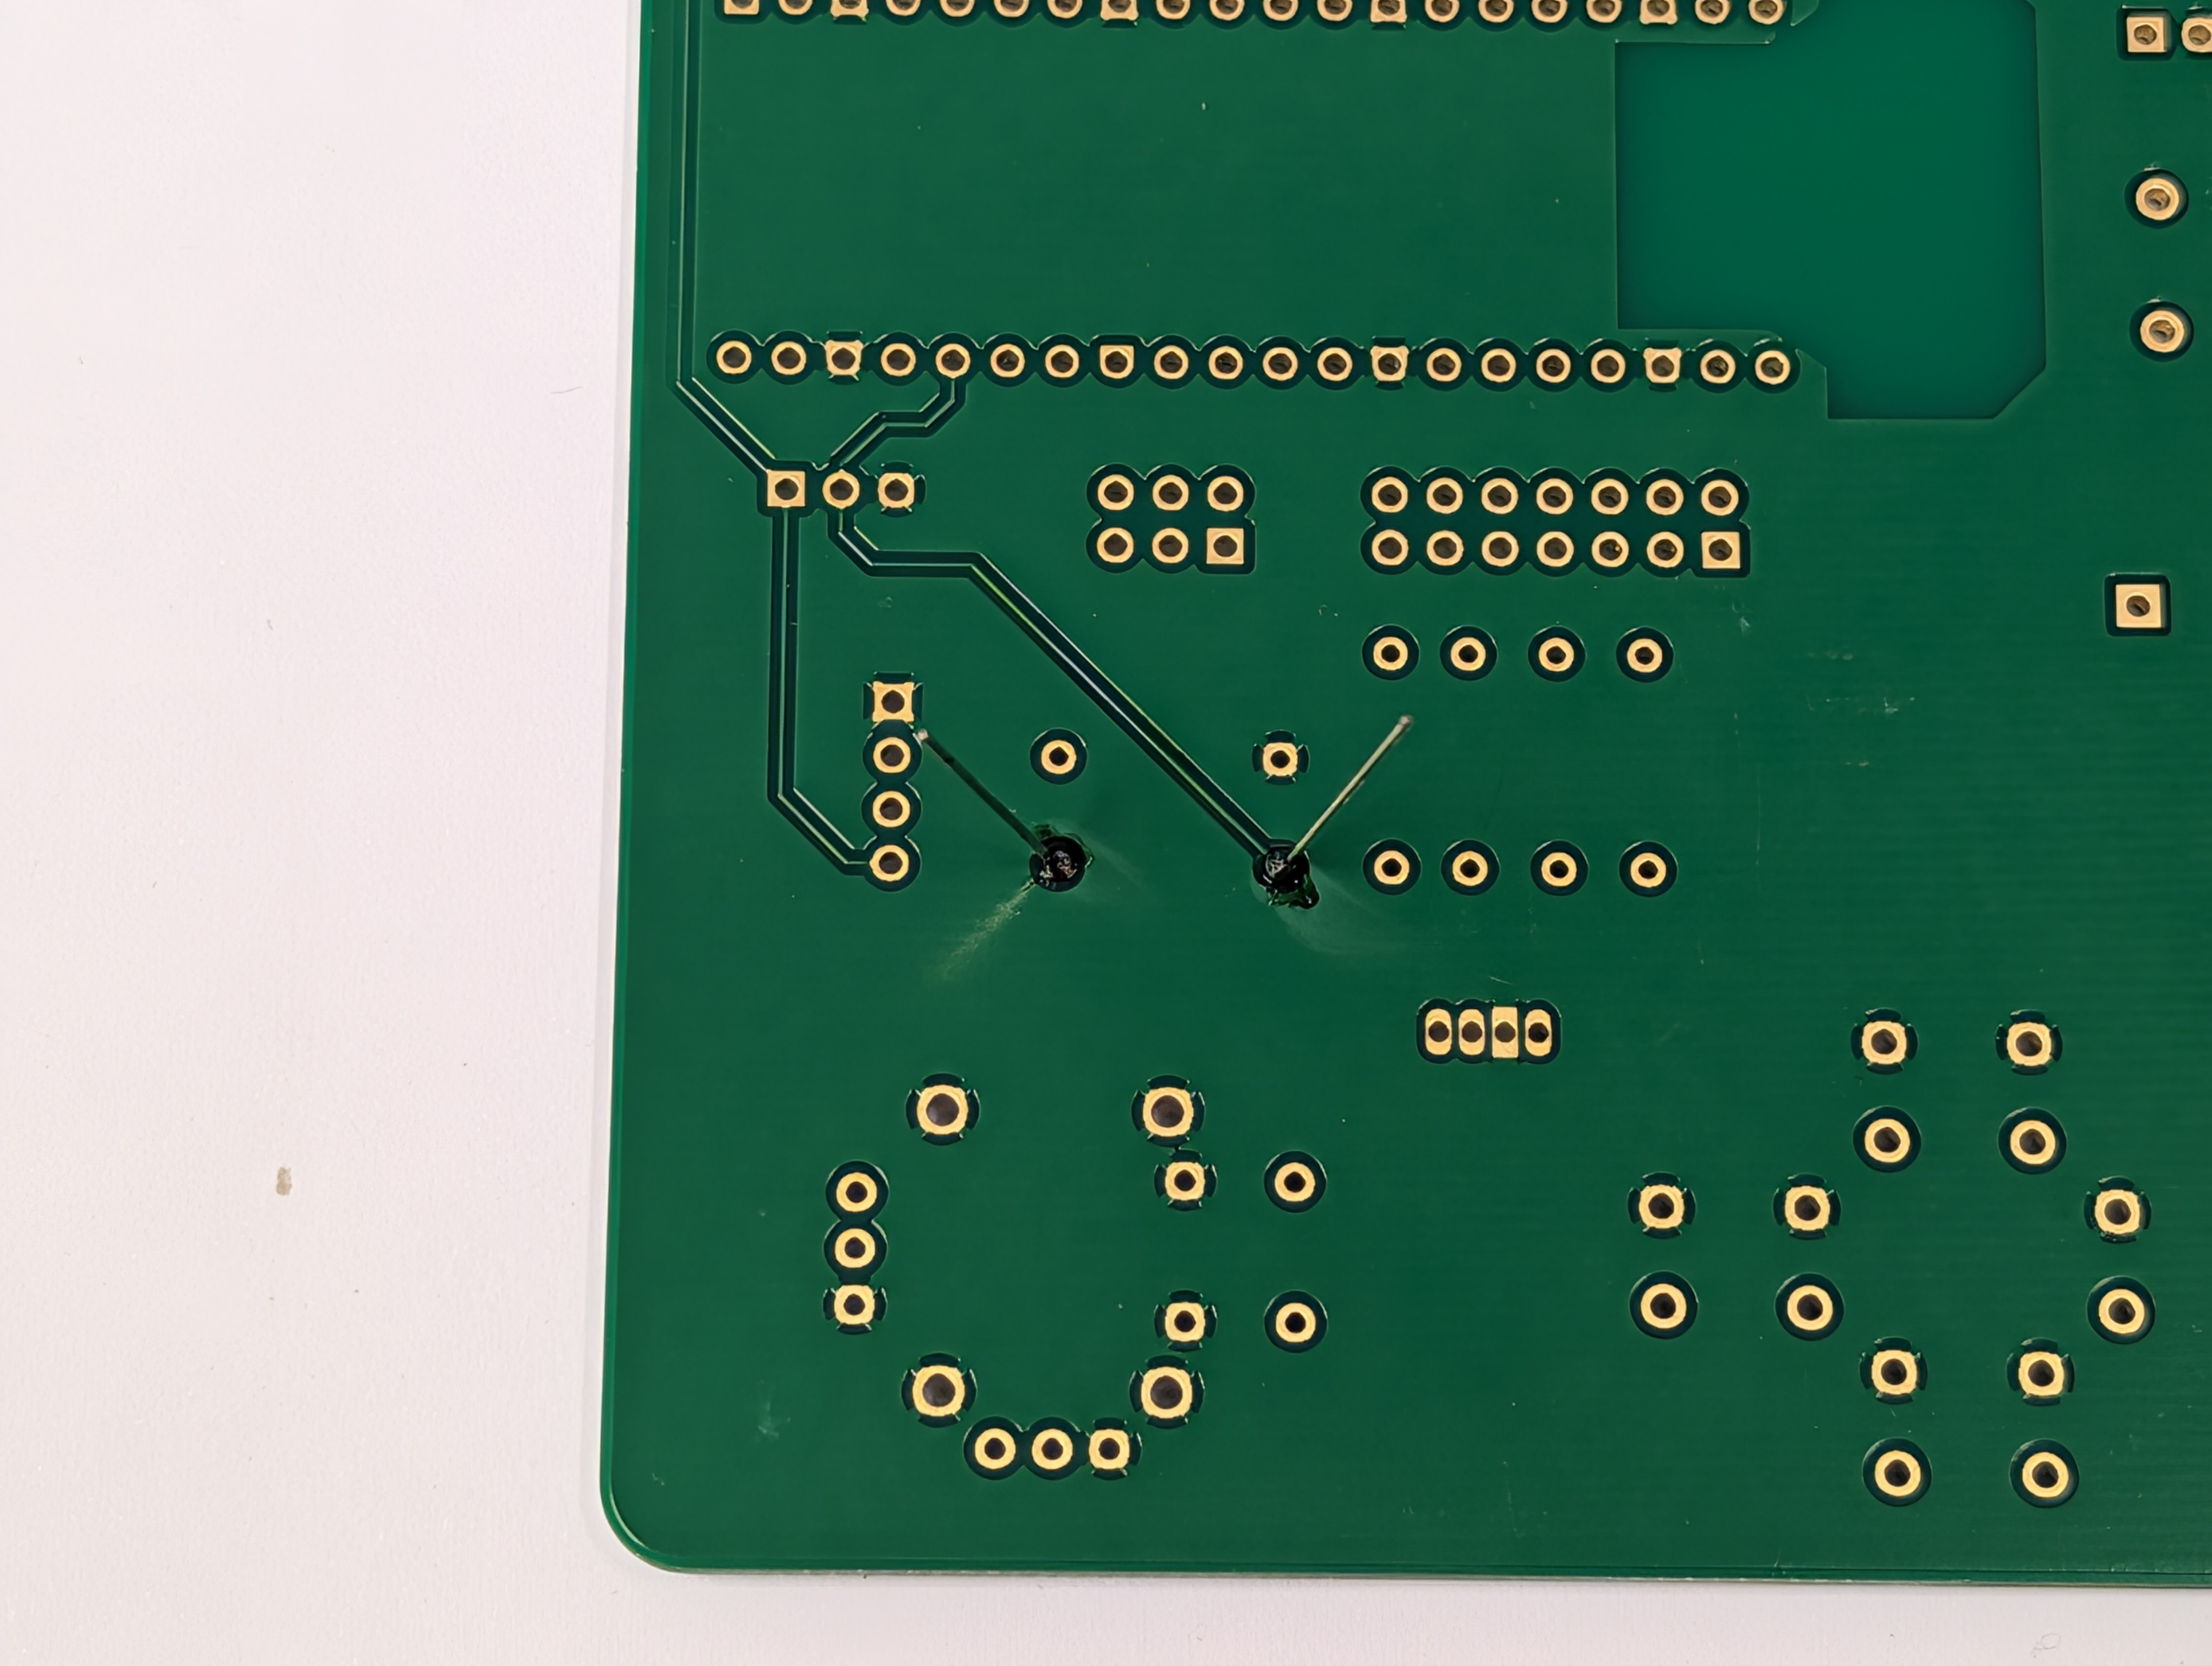
\includegraphics[width=0.75\textwidth]{pictures_of_construction/instruction_step_25.jpg}
\end{figure}

\begin{figure}[H]
    \centering
    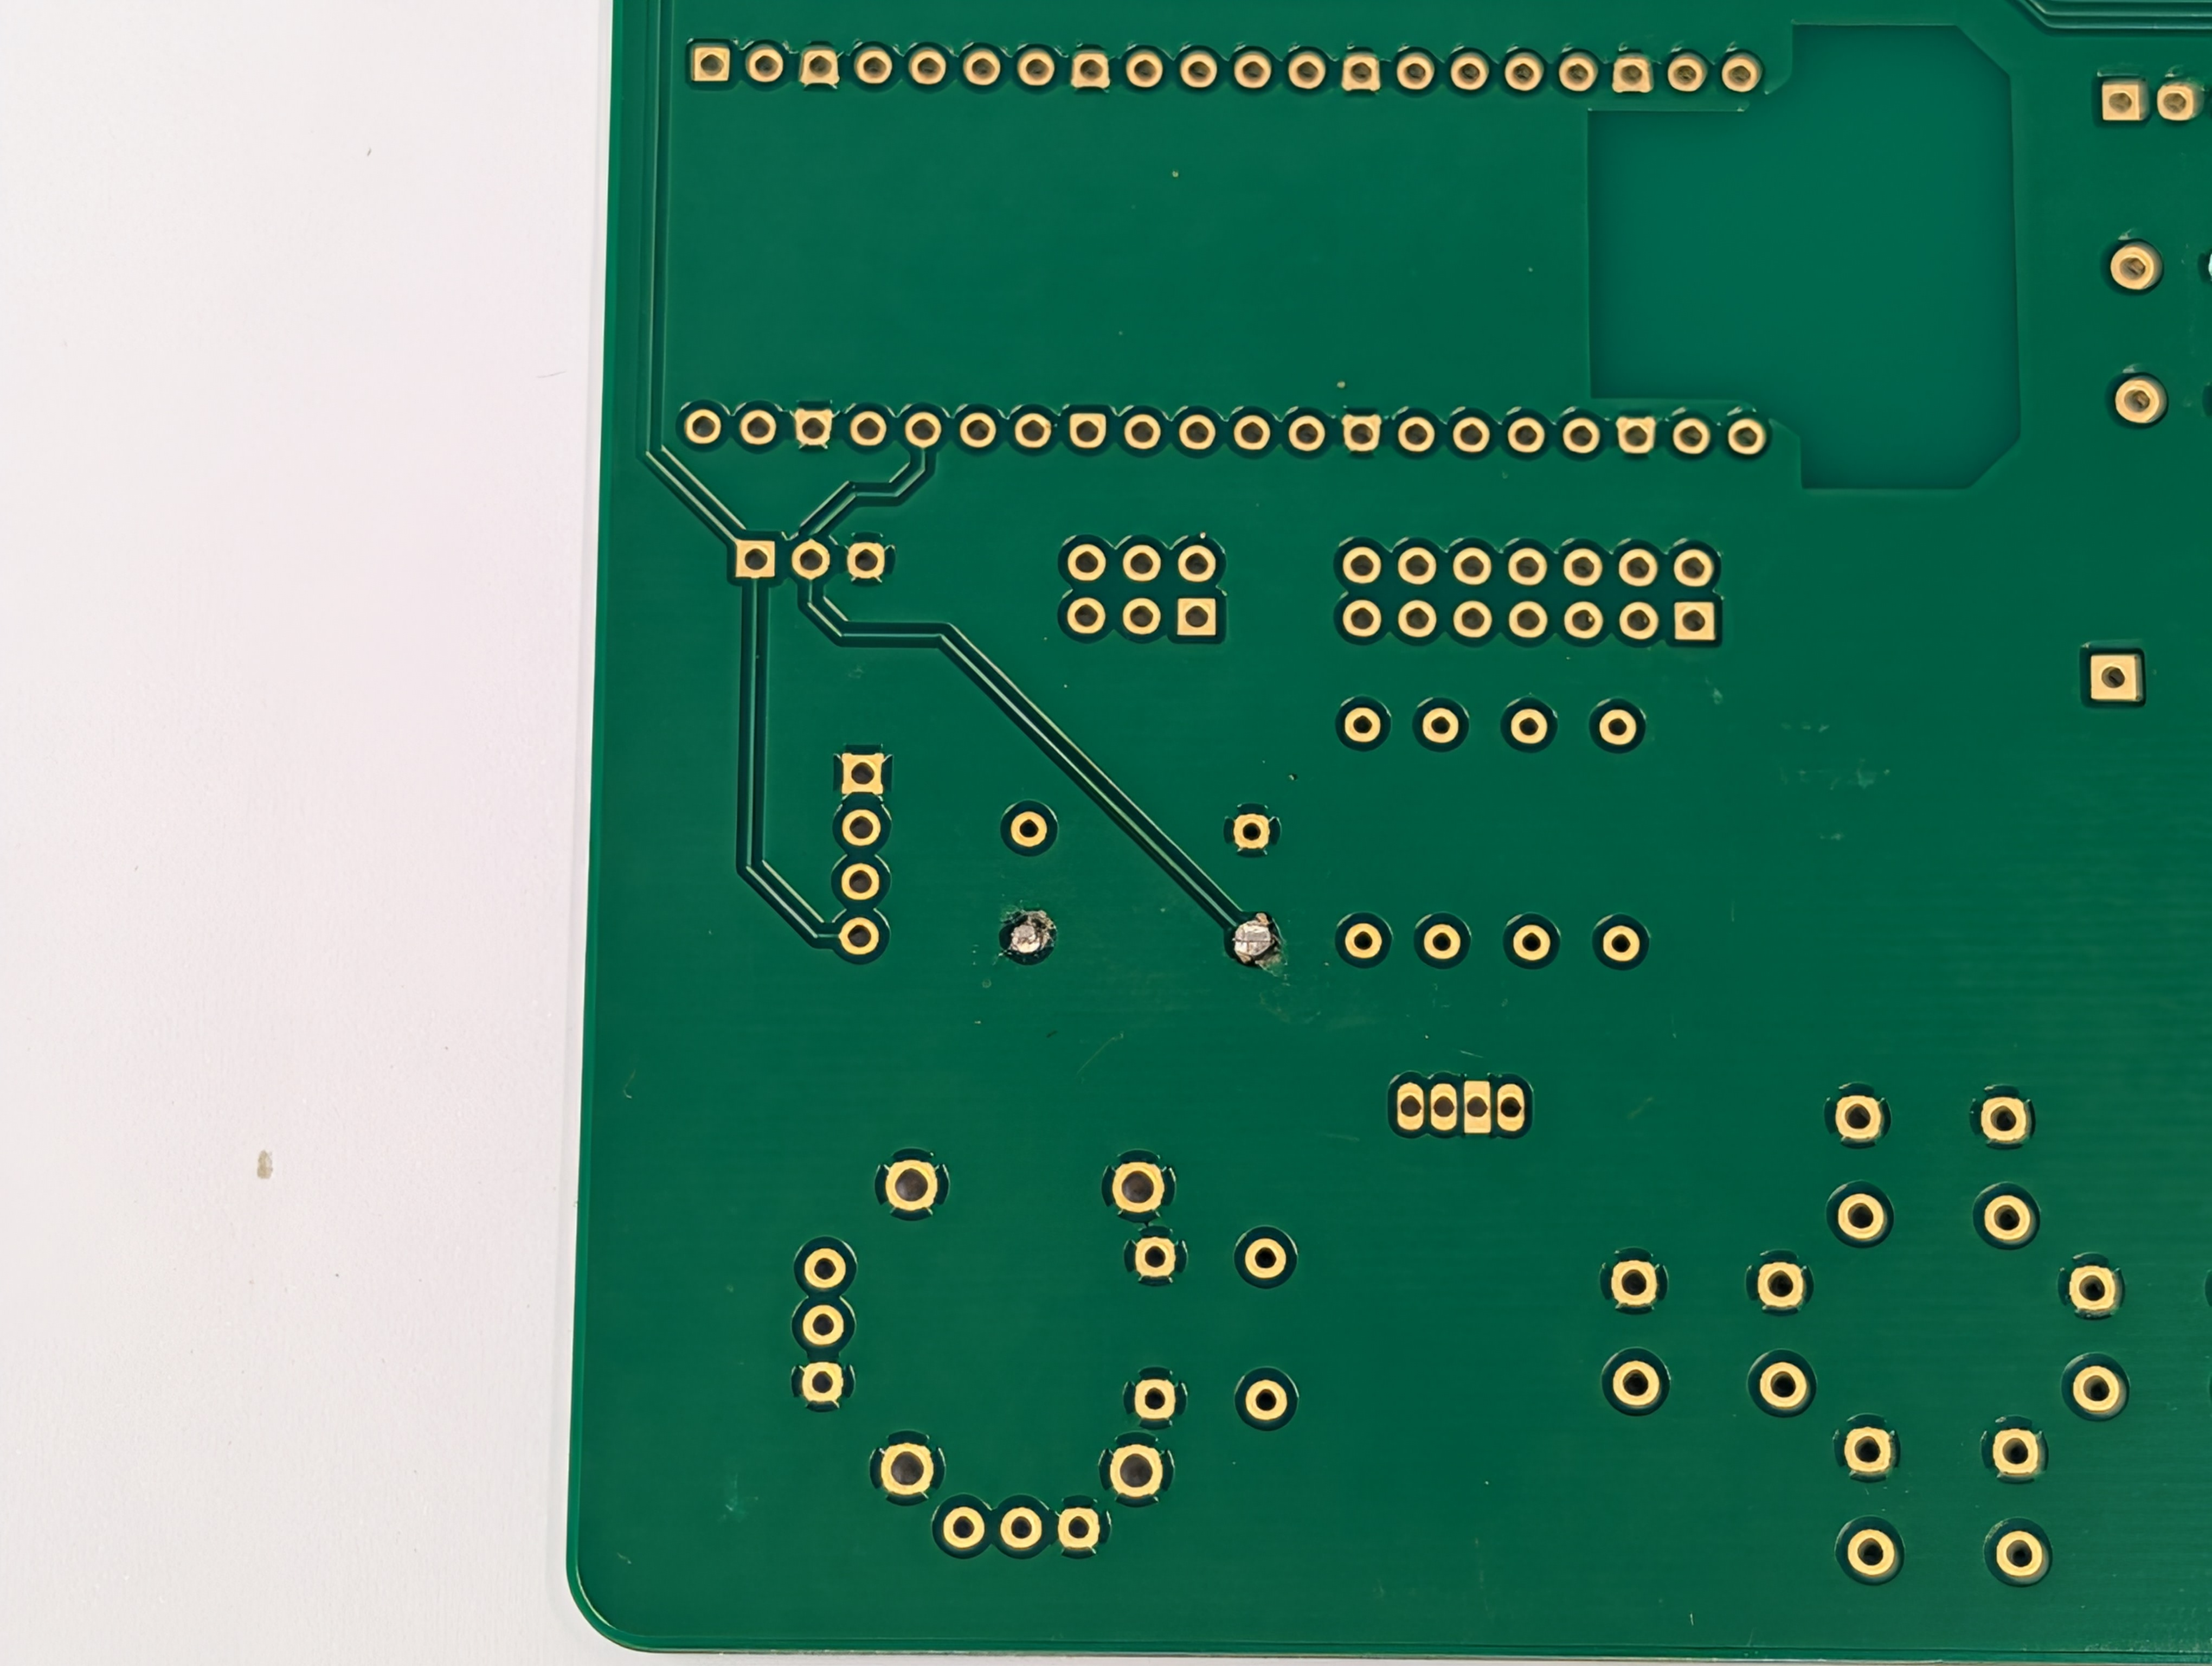
\includegraphics[width=0.75\textwidth]{pictures_of_construction/instruction_step_26.jpg}
\end{figure}

After the resistor is fully seated, you can clip the leads flush with side cutters.

\subsubsection*{1 k$\Omega$ resistor}

The 1 k$\Omega$ resistor has stripes as markings (Brown | Black | Red | Gold).

\begin{figure}[H]
    \centering
    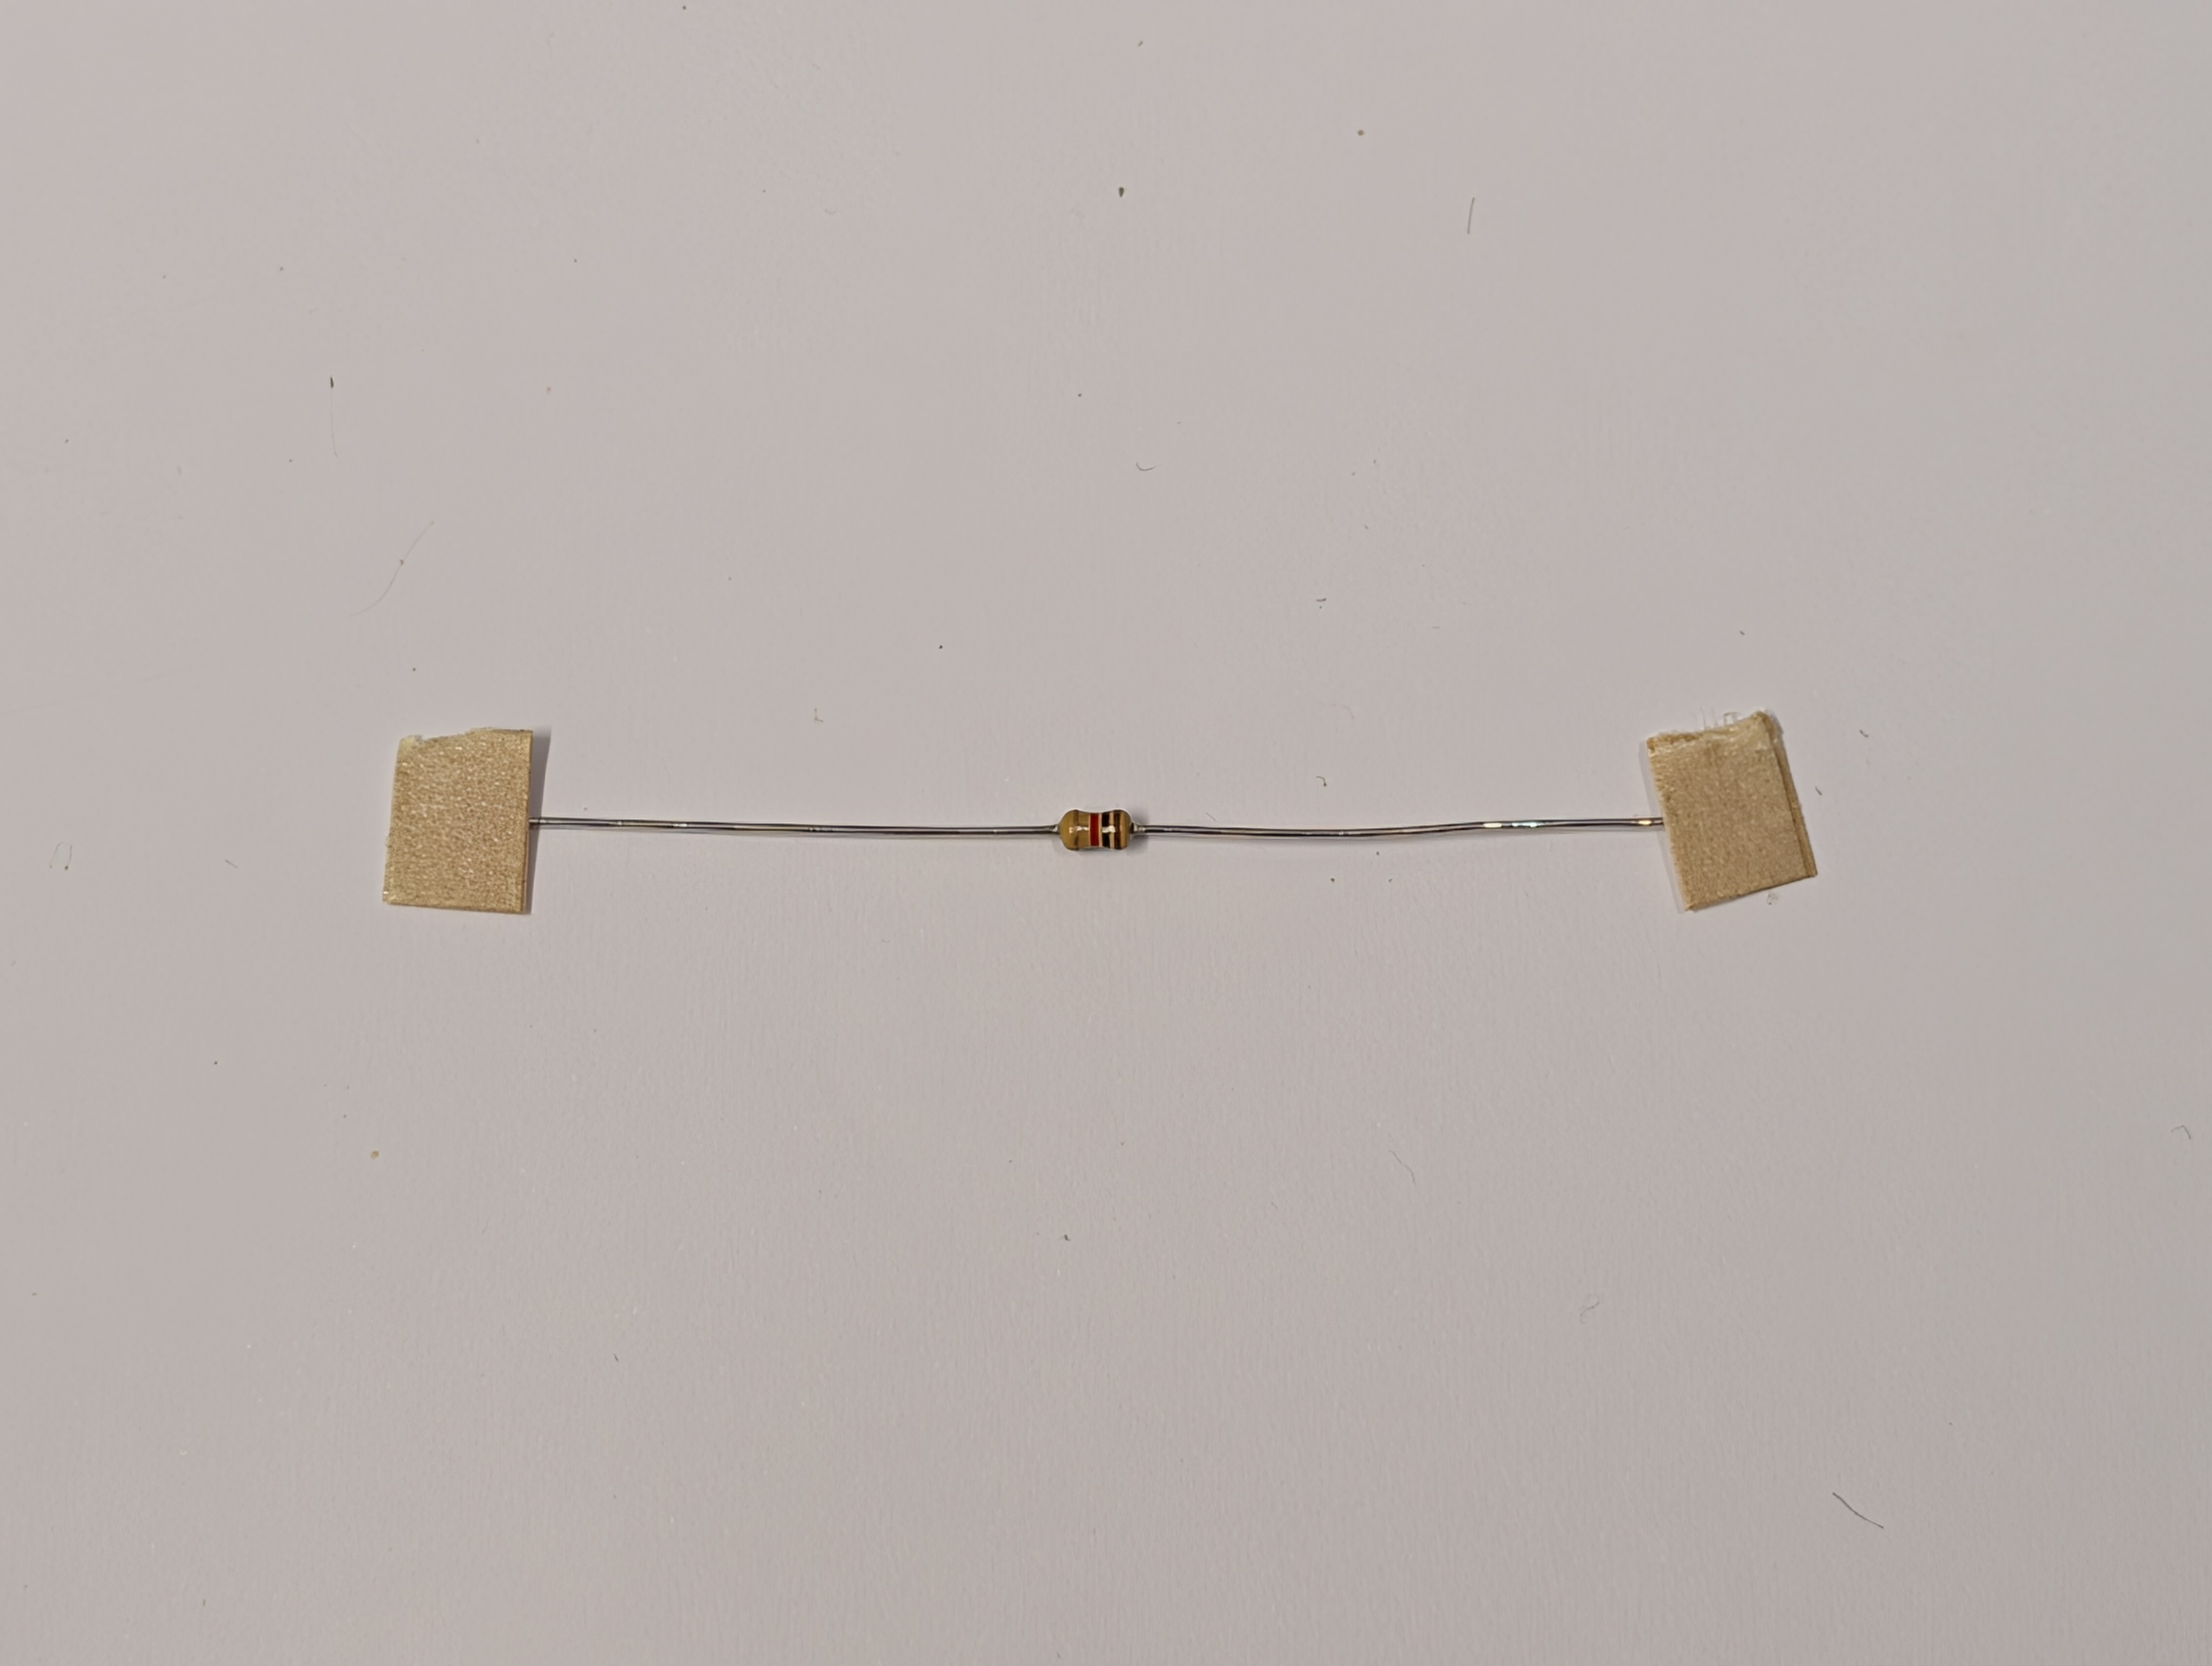
\includegraphics[width=0.75\textwidth]{pictures_of_construction/instruction_step_27.jpg}
\end{figure}

\begin{figure}[H]
    \centering
    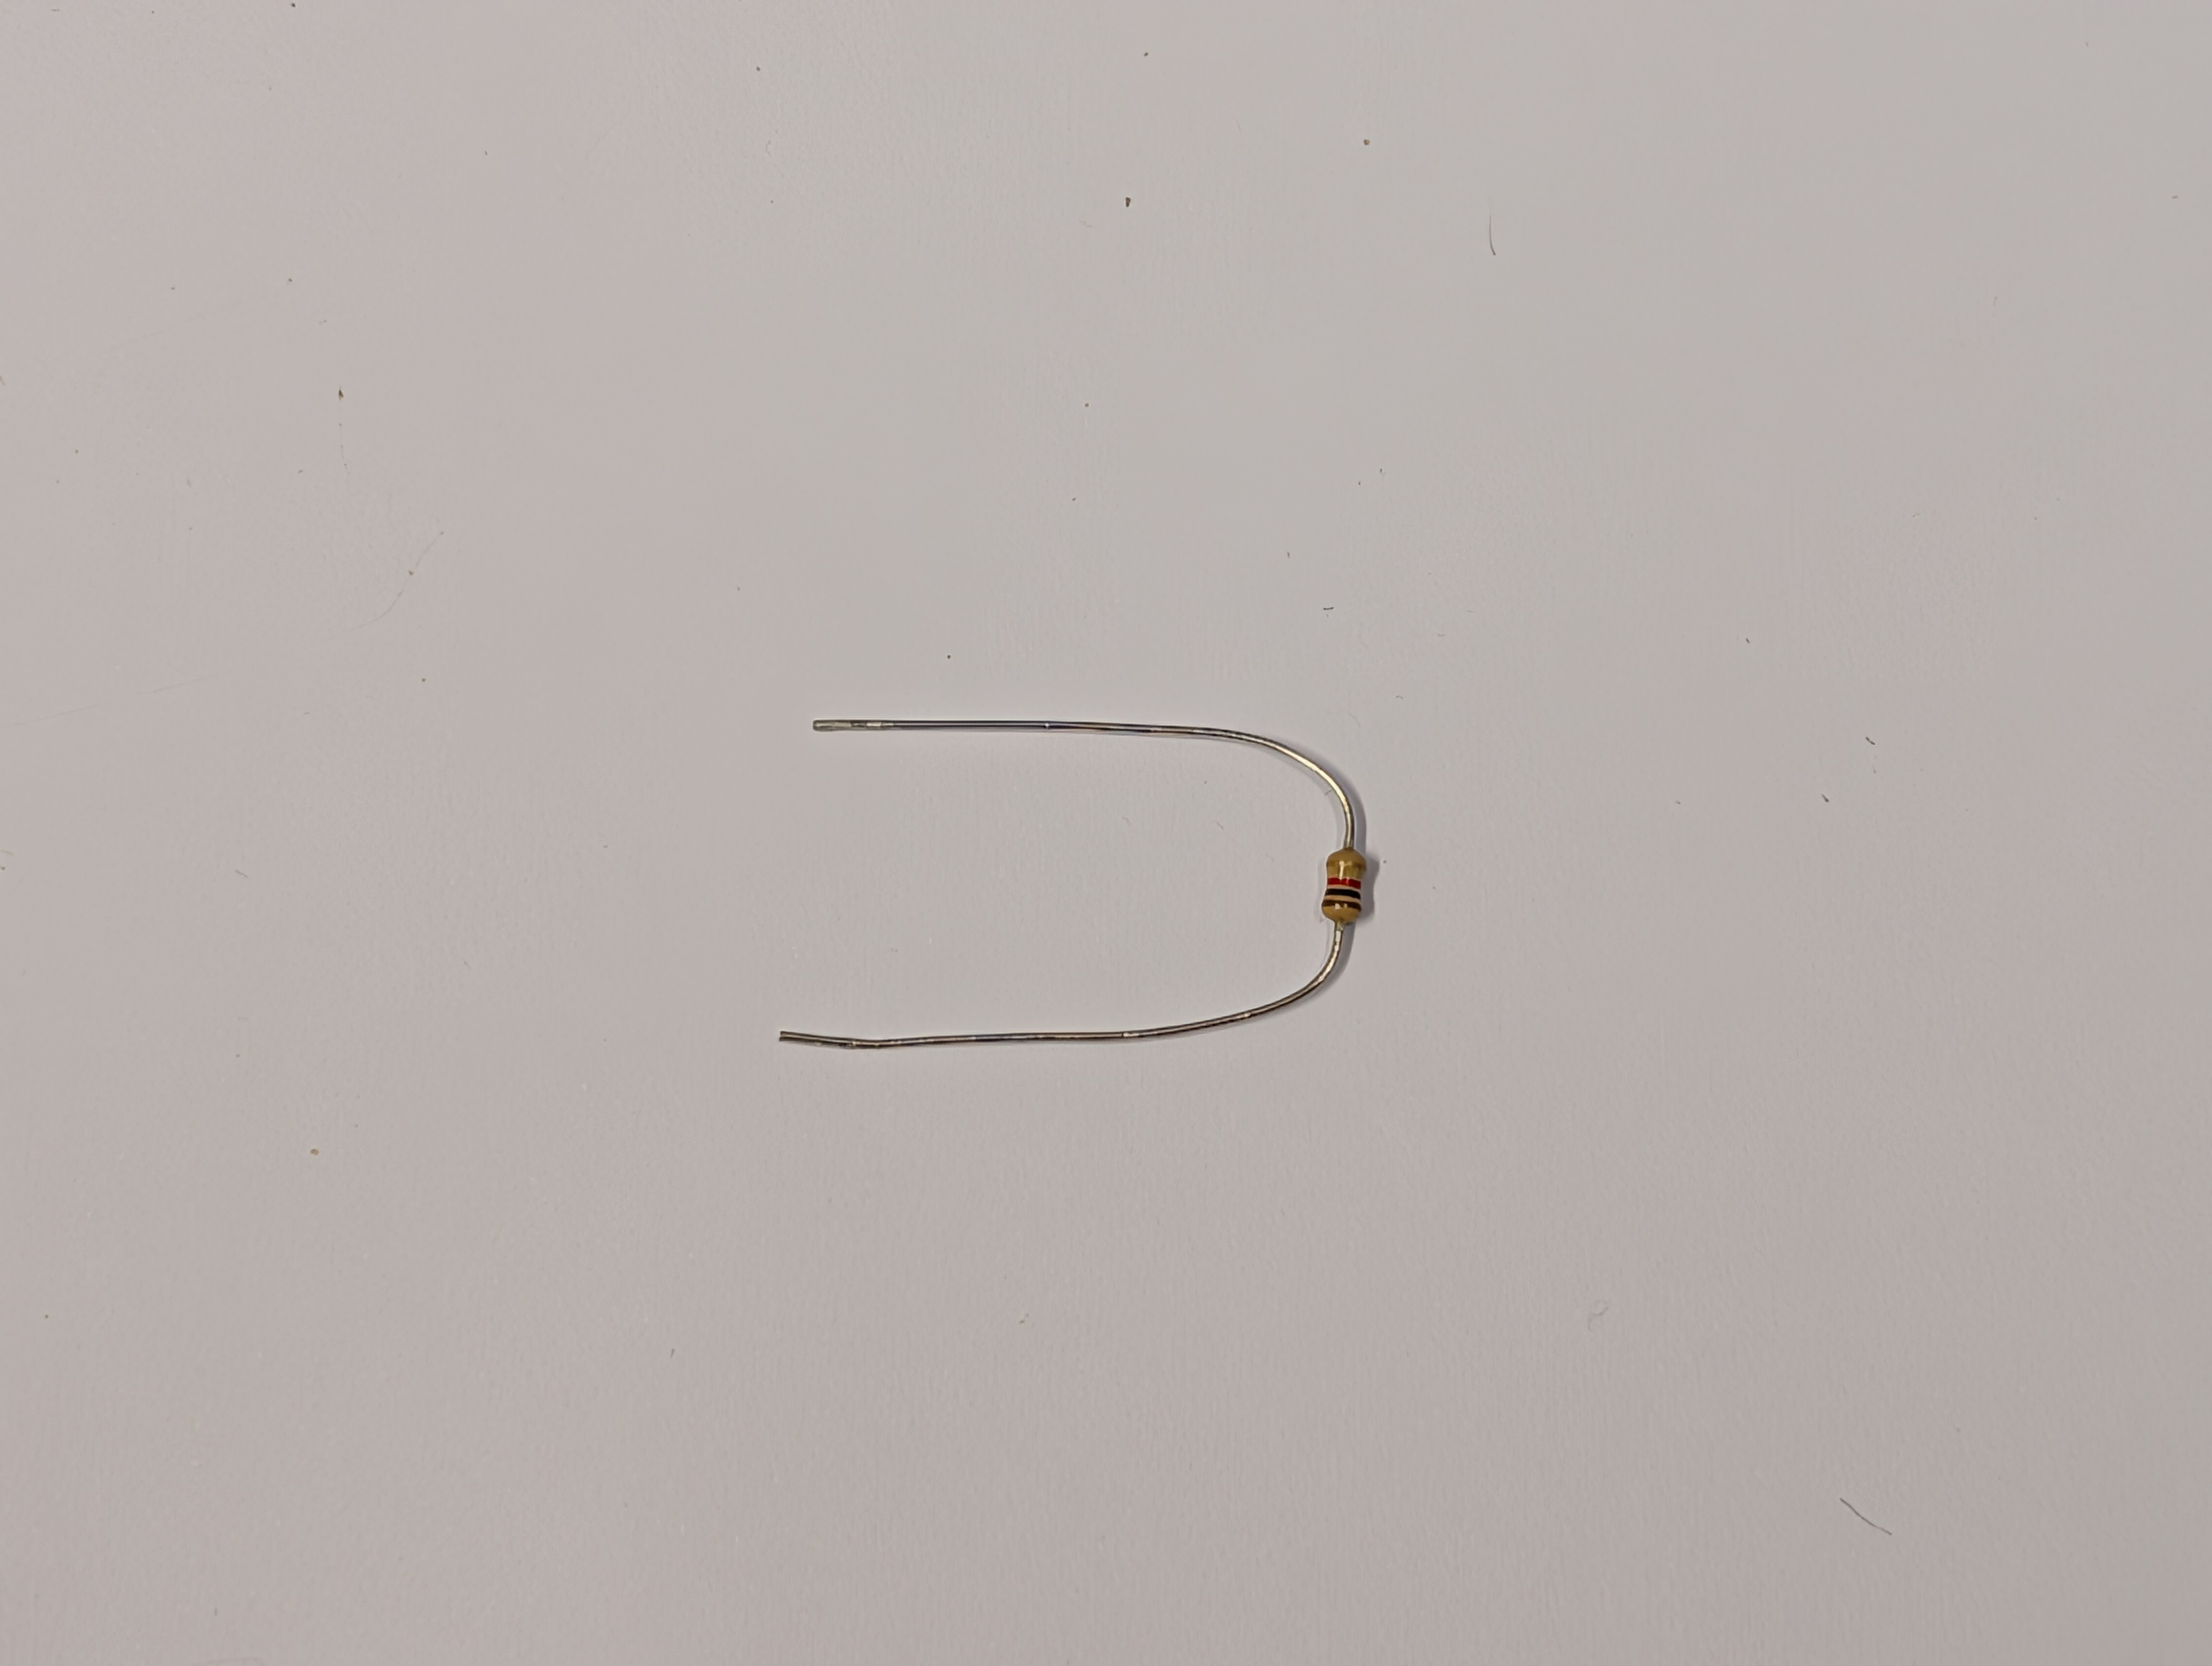
\includegraphics[width=0.75\textwidth]{pictures_of_construction/instruction_step_28.jpg}
\end{figure}

The installation of the different resistors is essentially identical. For the 1 k$\Omega$ resistor, start by forming it roughly U-shaped.

\begin{figure}[H]
    \centering
    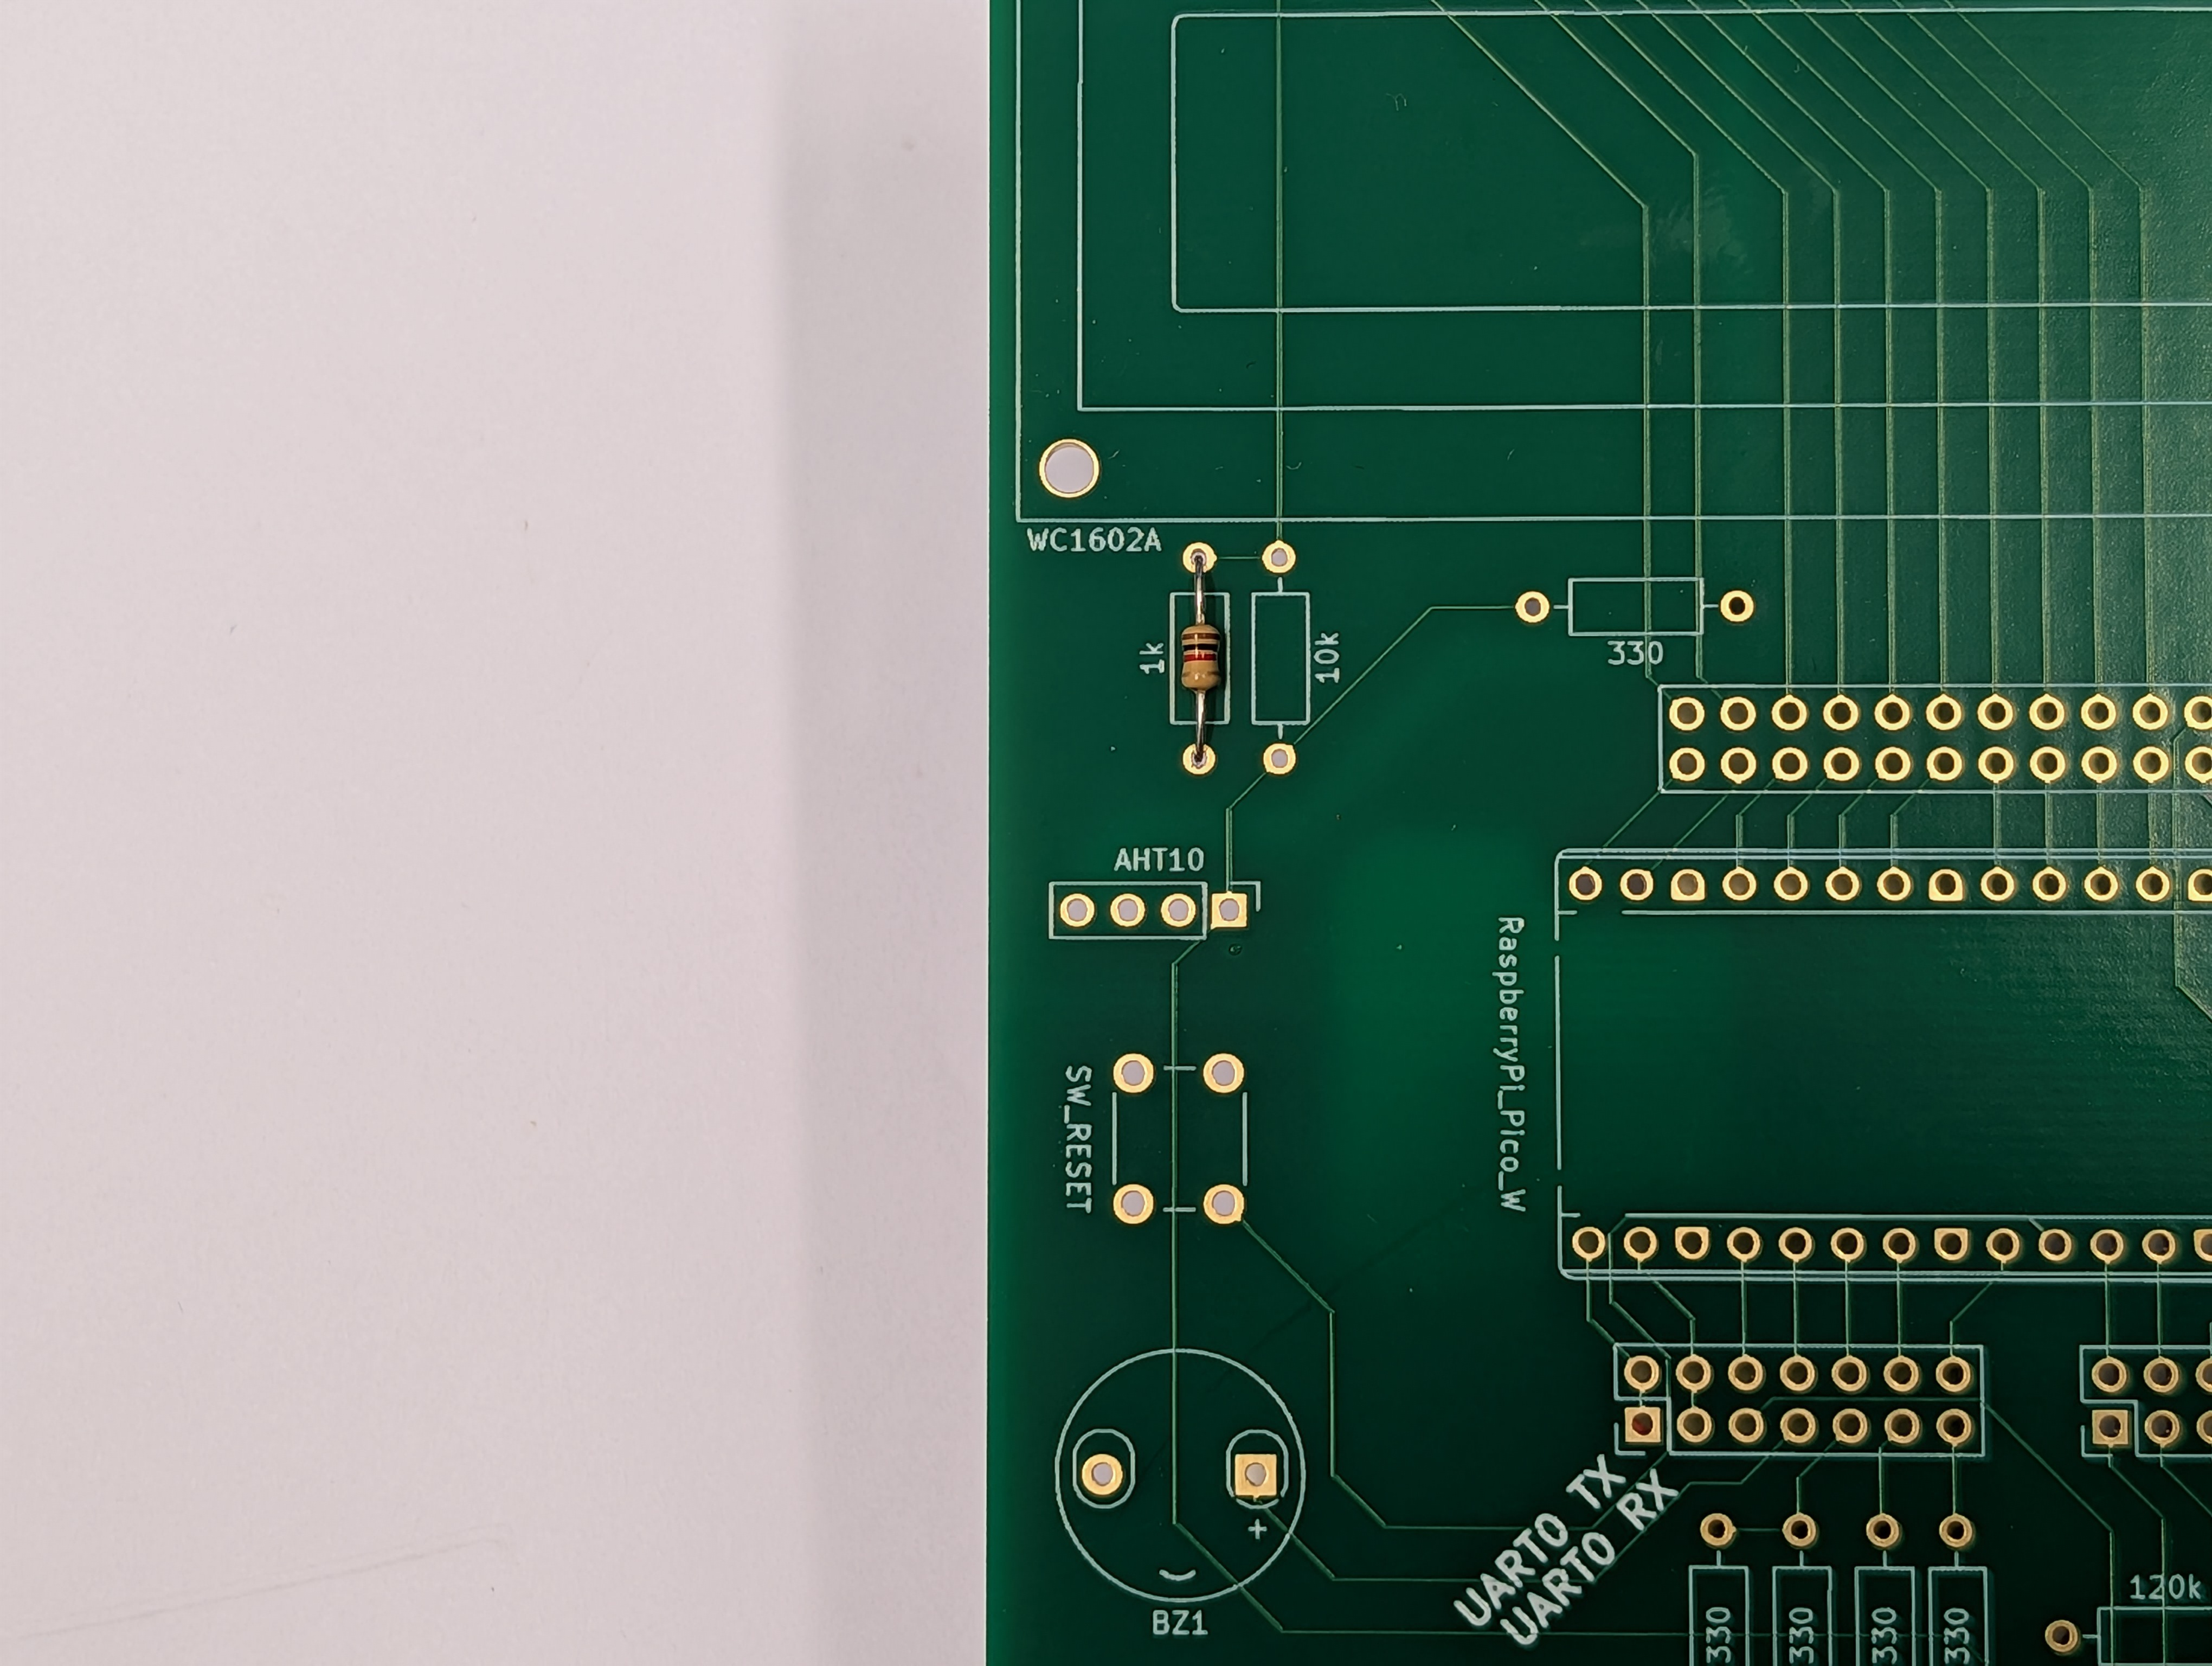
\includegraphics[width=0.75\textwidth]{pictures_of_construction/instruction_step_29.jpg}
\end{figure}

Then place it in its position, solder one leg, correct the placement, solder completely, and clip the leads flush.

\subsubsection*{10 k$\Omega$ resistor}

The 10 k$\Omega$ resistor has stripes as markings (Brown | Black | Orange | Gold).

\begin{figure}[H]
    \centering
    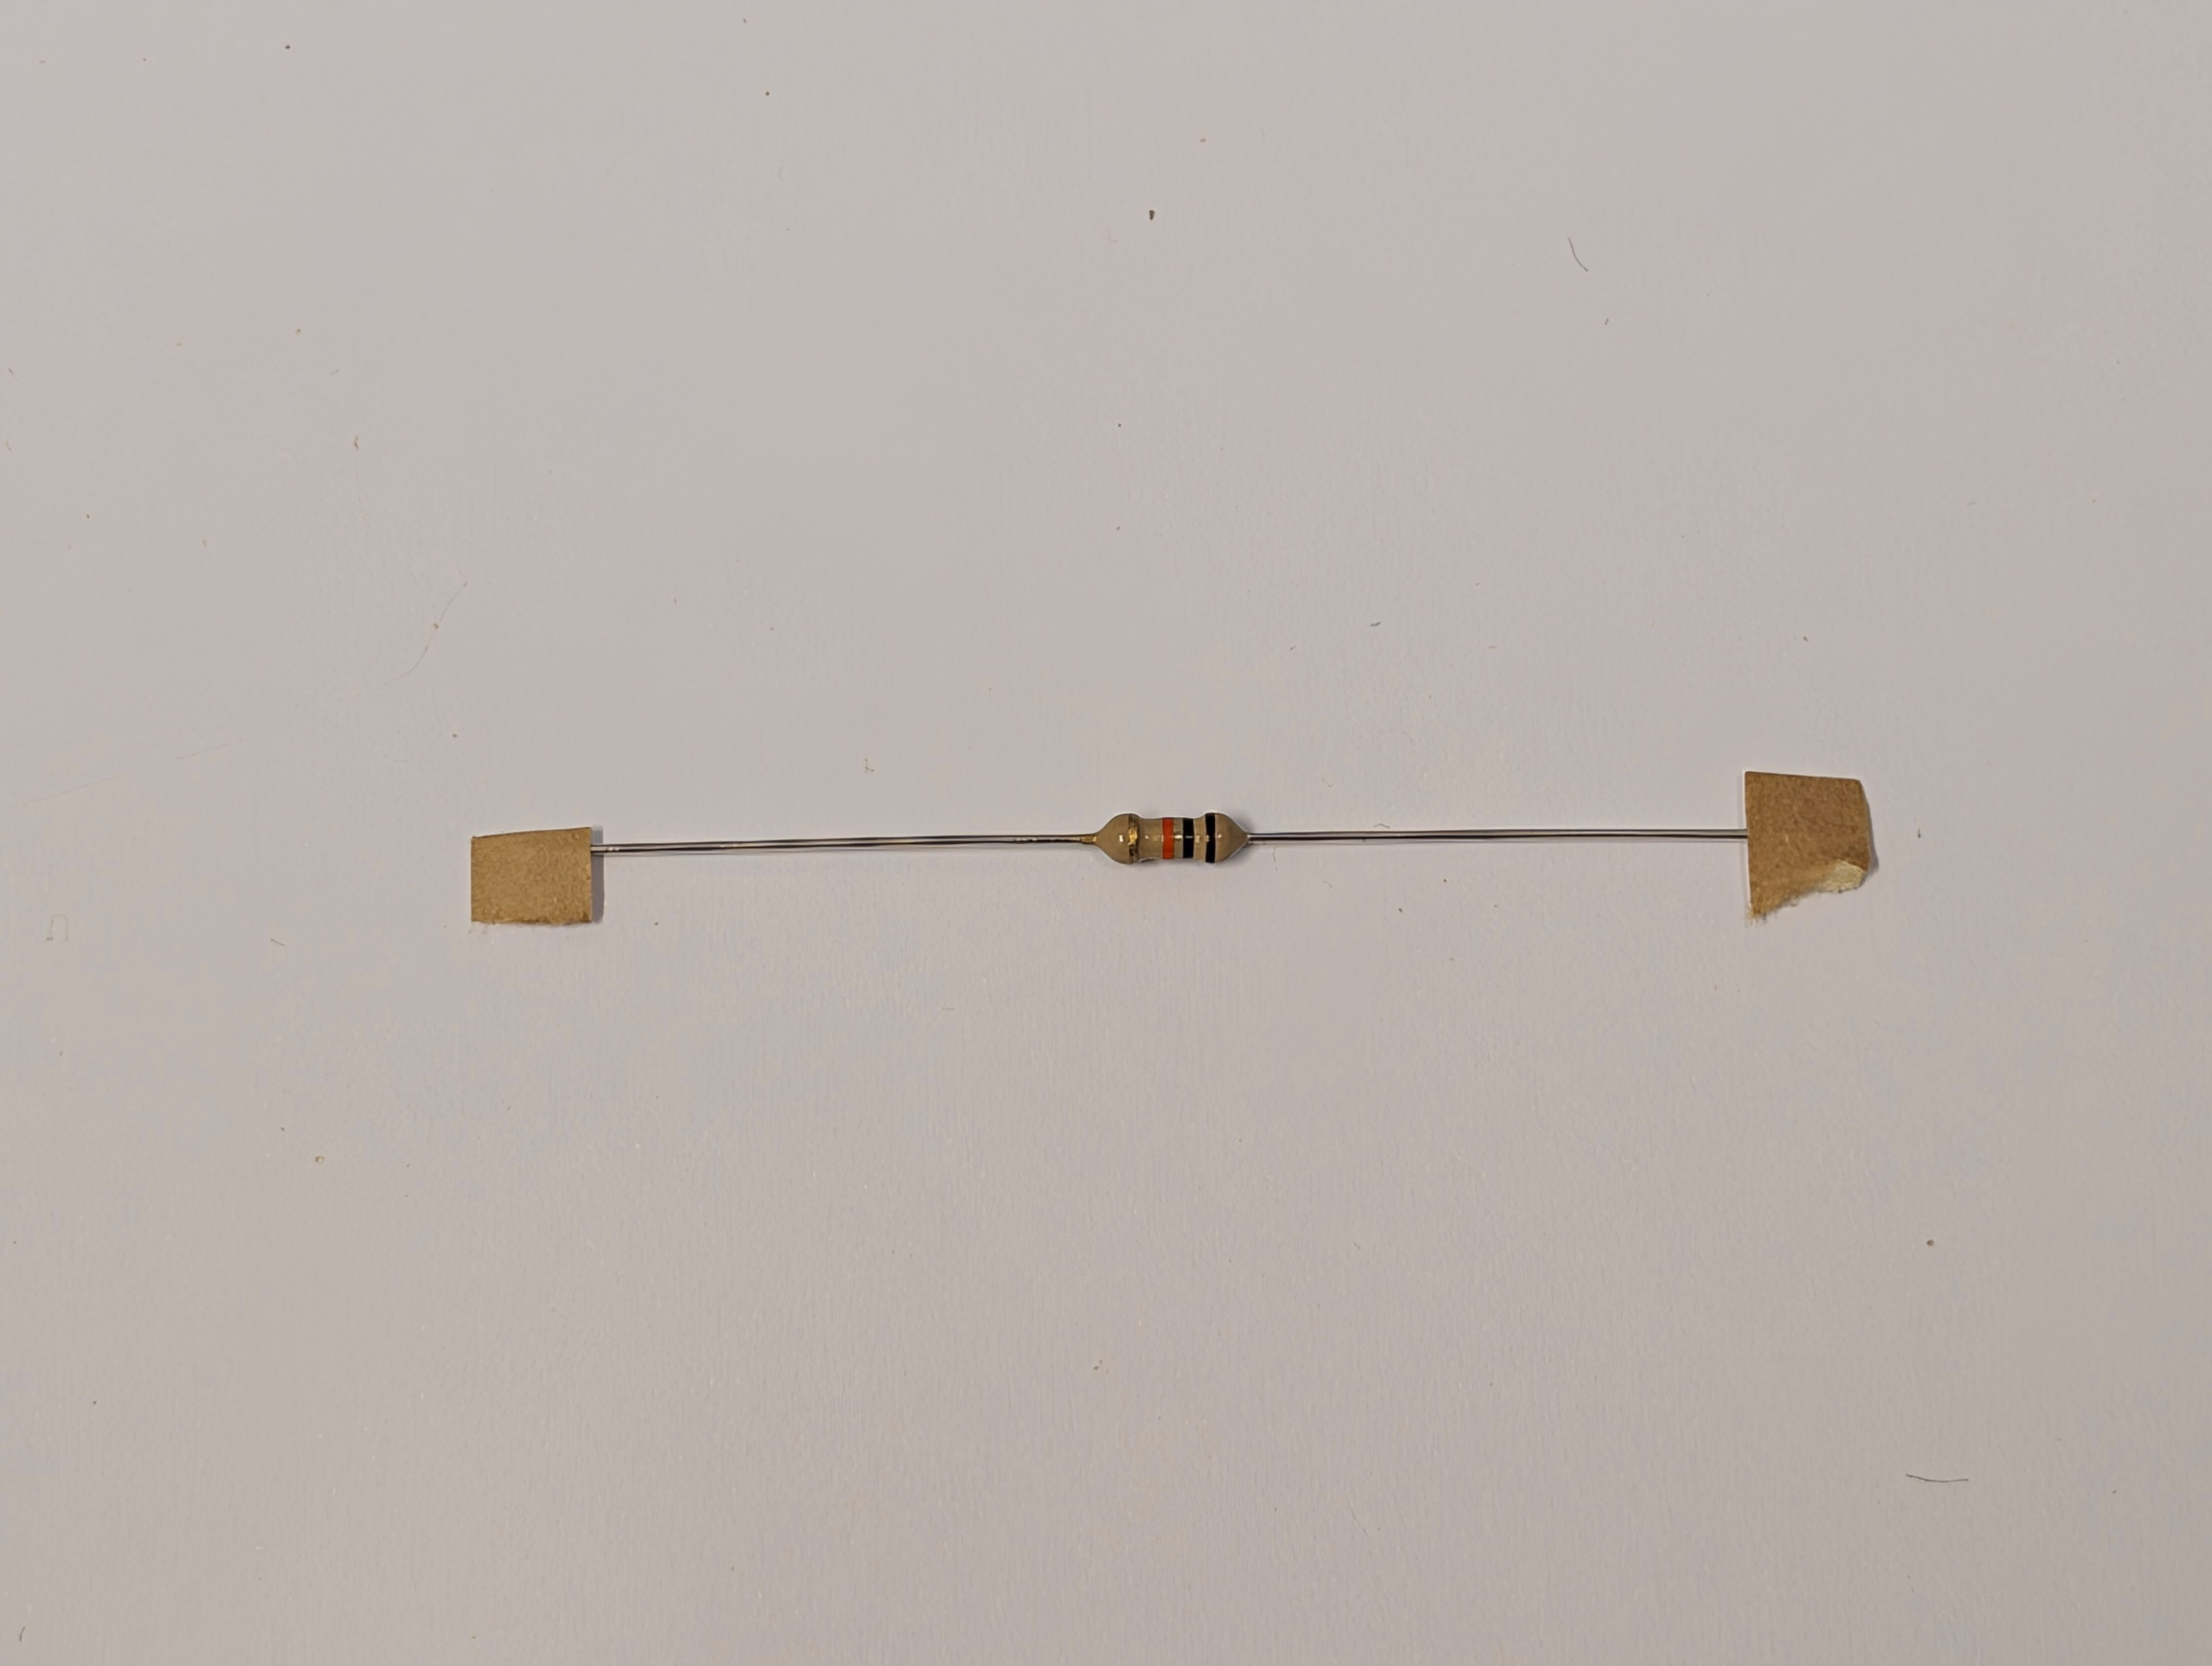
\includegraphics[width=0.75\textwidth]{pictures_of_construction/instruction_step_30.jpg}
\end{figure}

\begin{figure}[H]
    \centering
    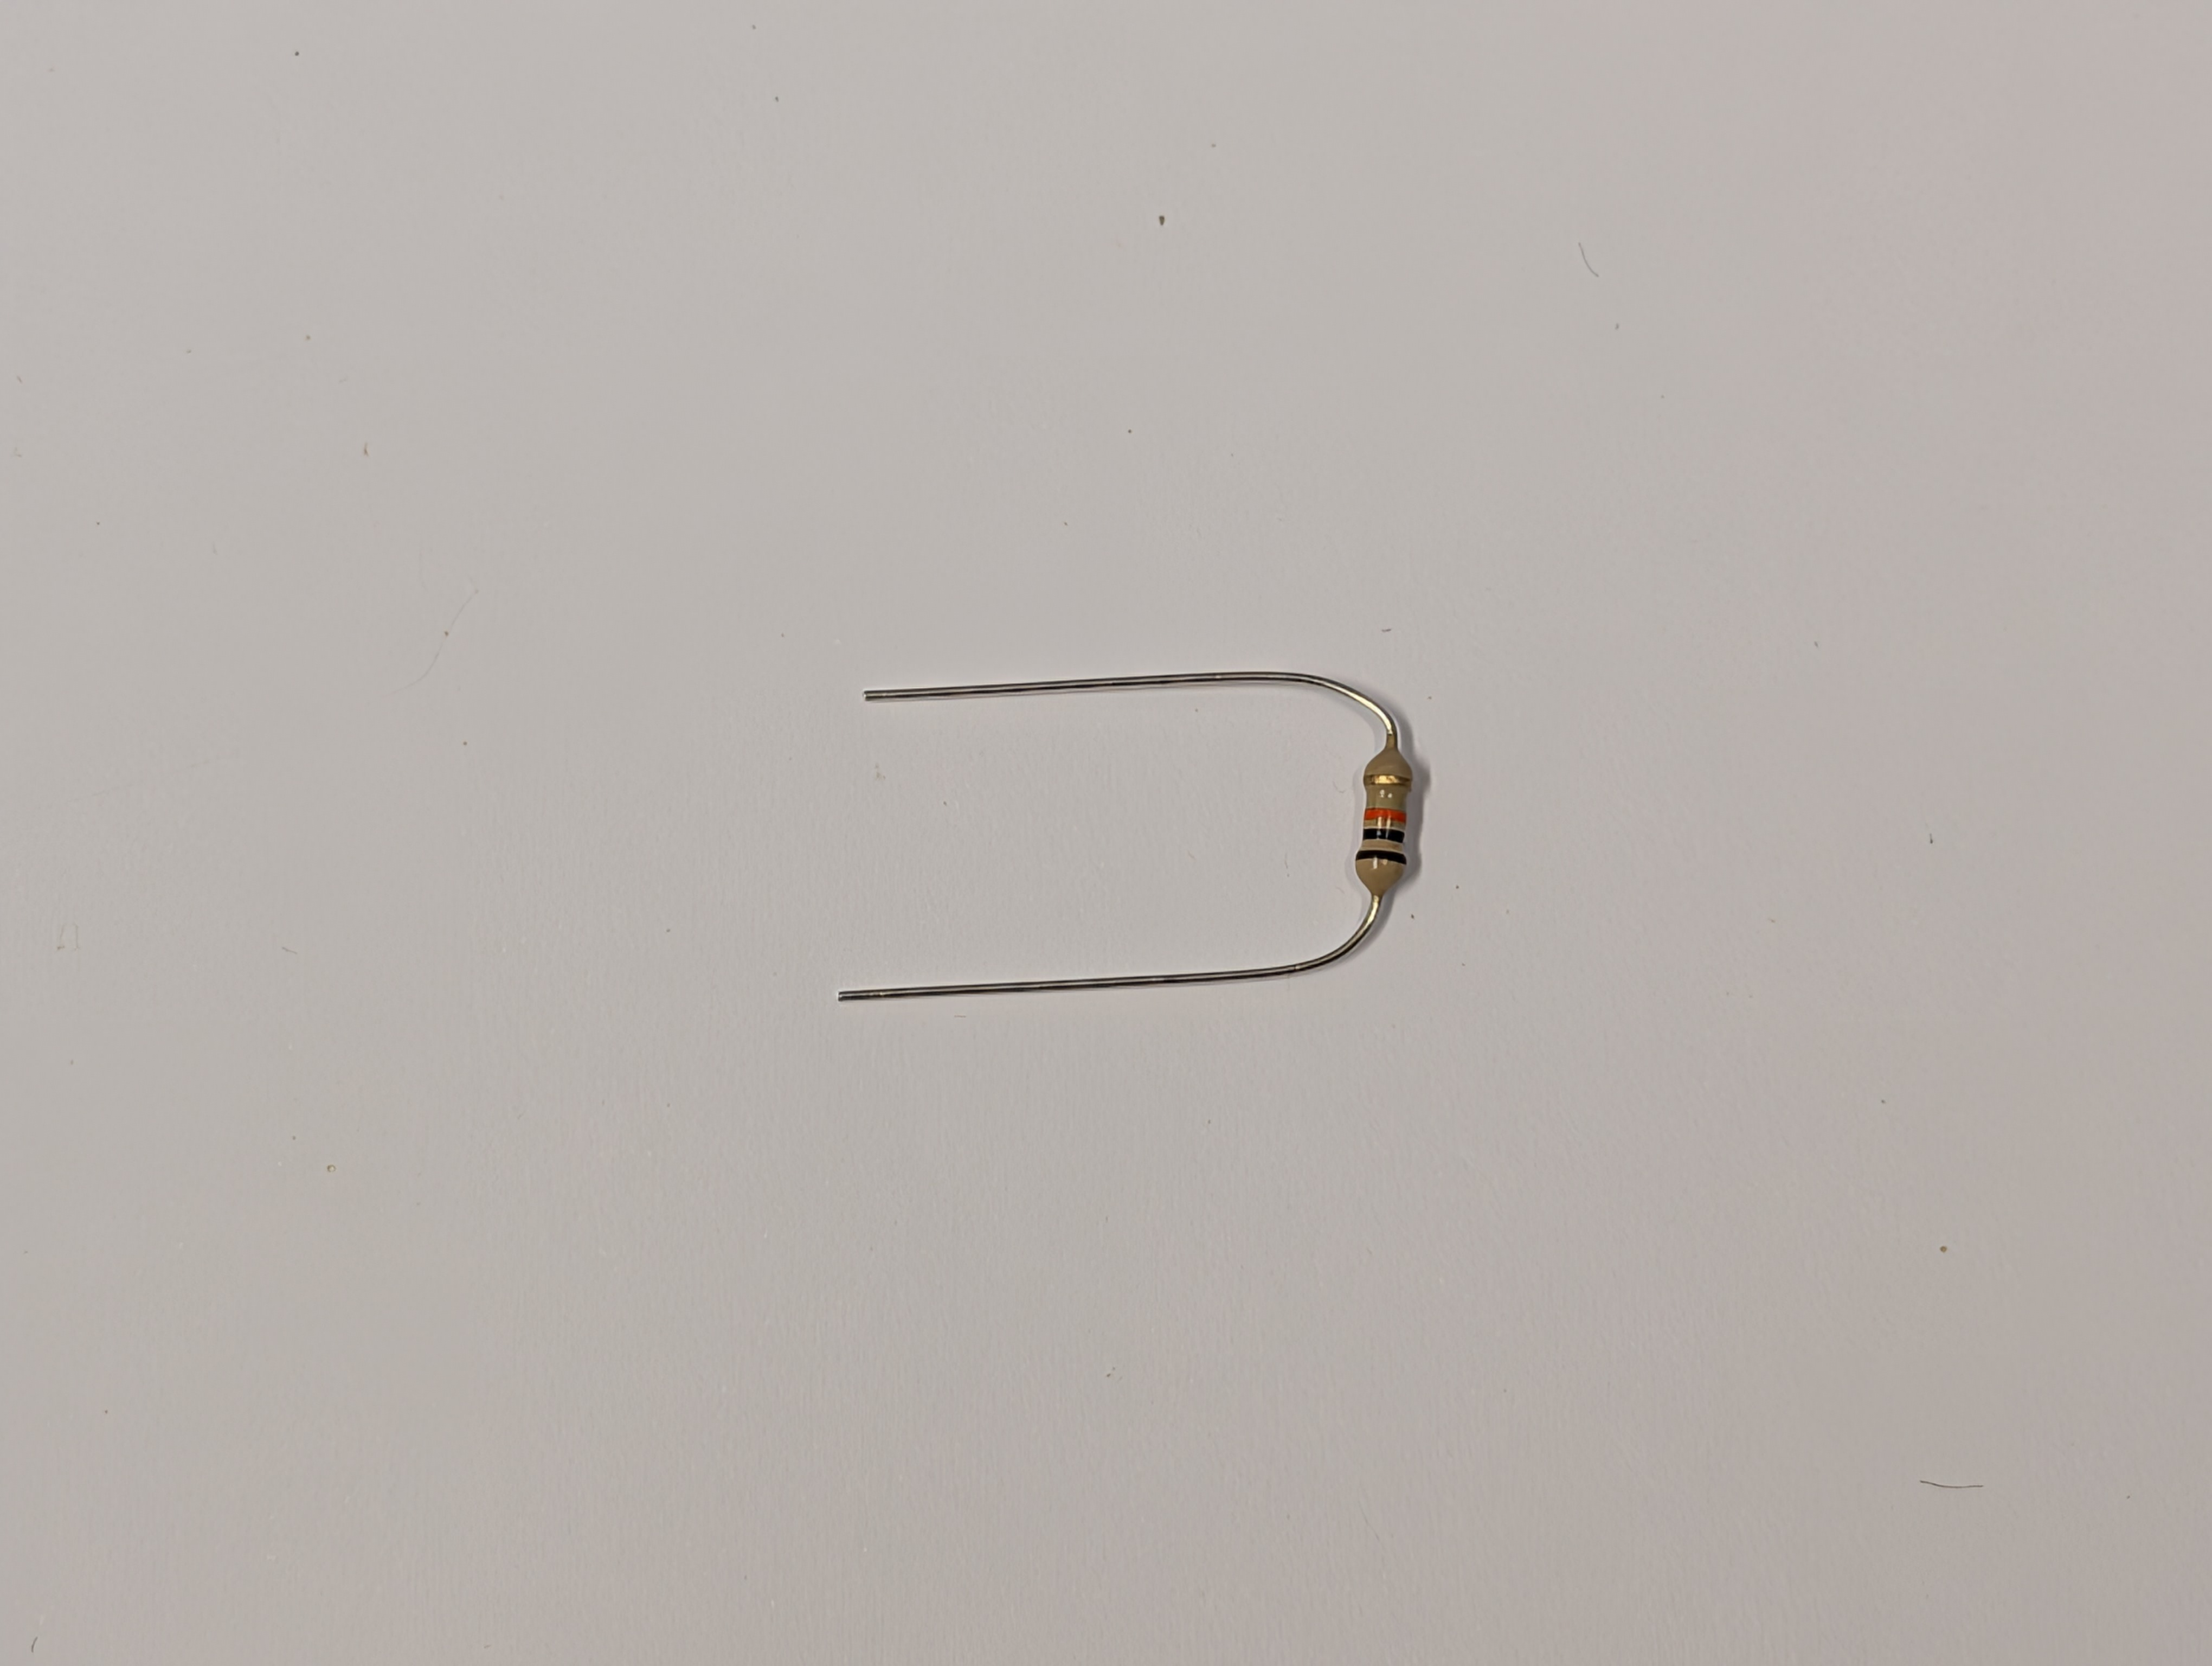
\includegraphics[width=0.75\textwidth]{pictures_of_construction/instruction_step_31.jpg}
\end{figure}

\begin{figure}[H]
    \centering
    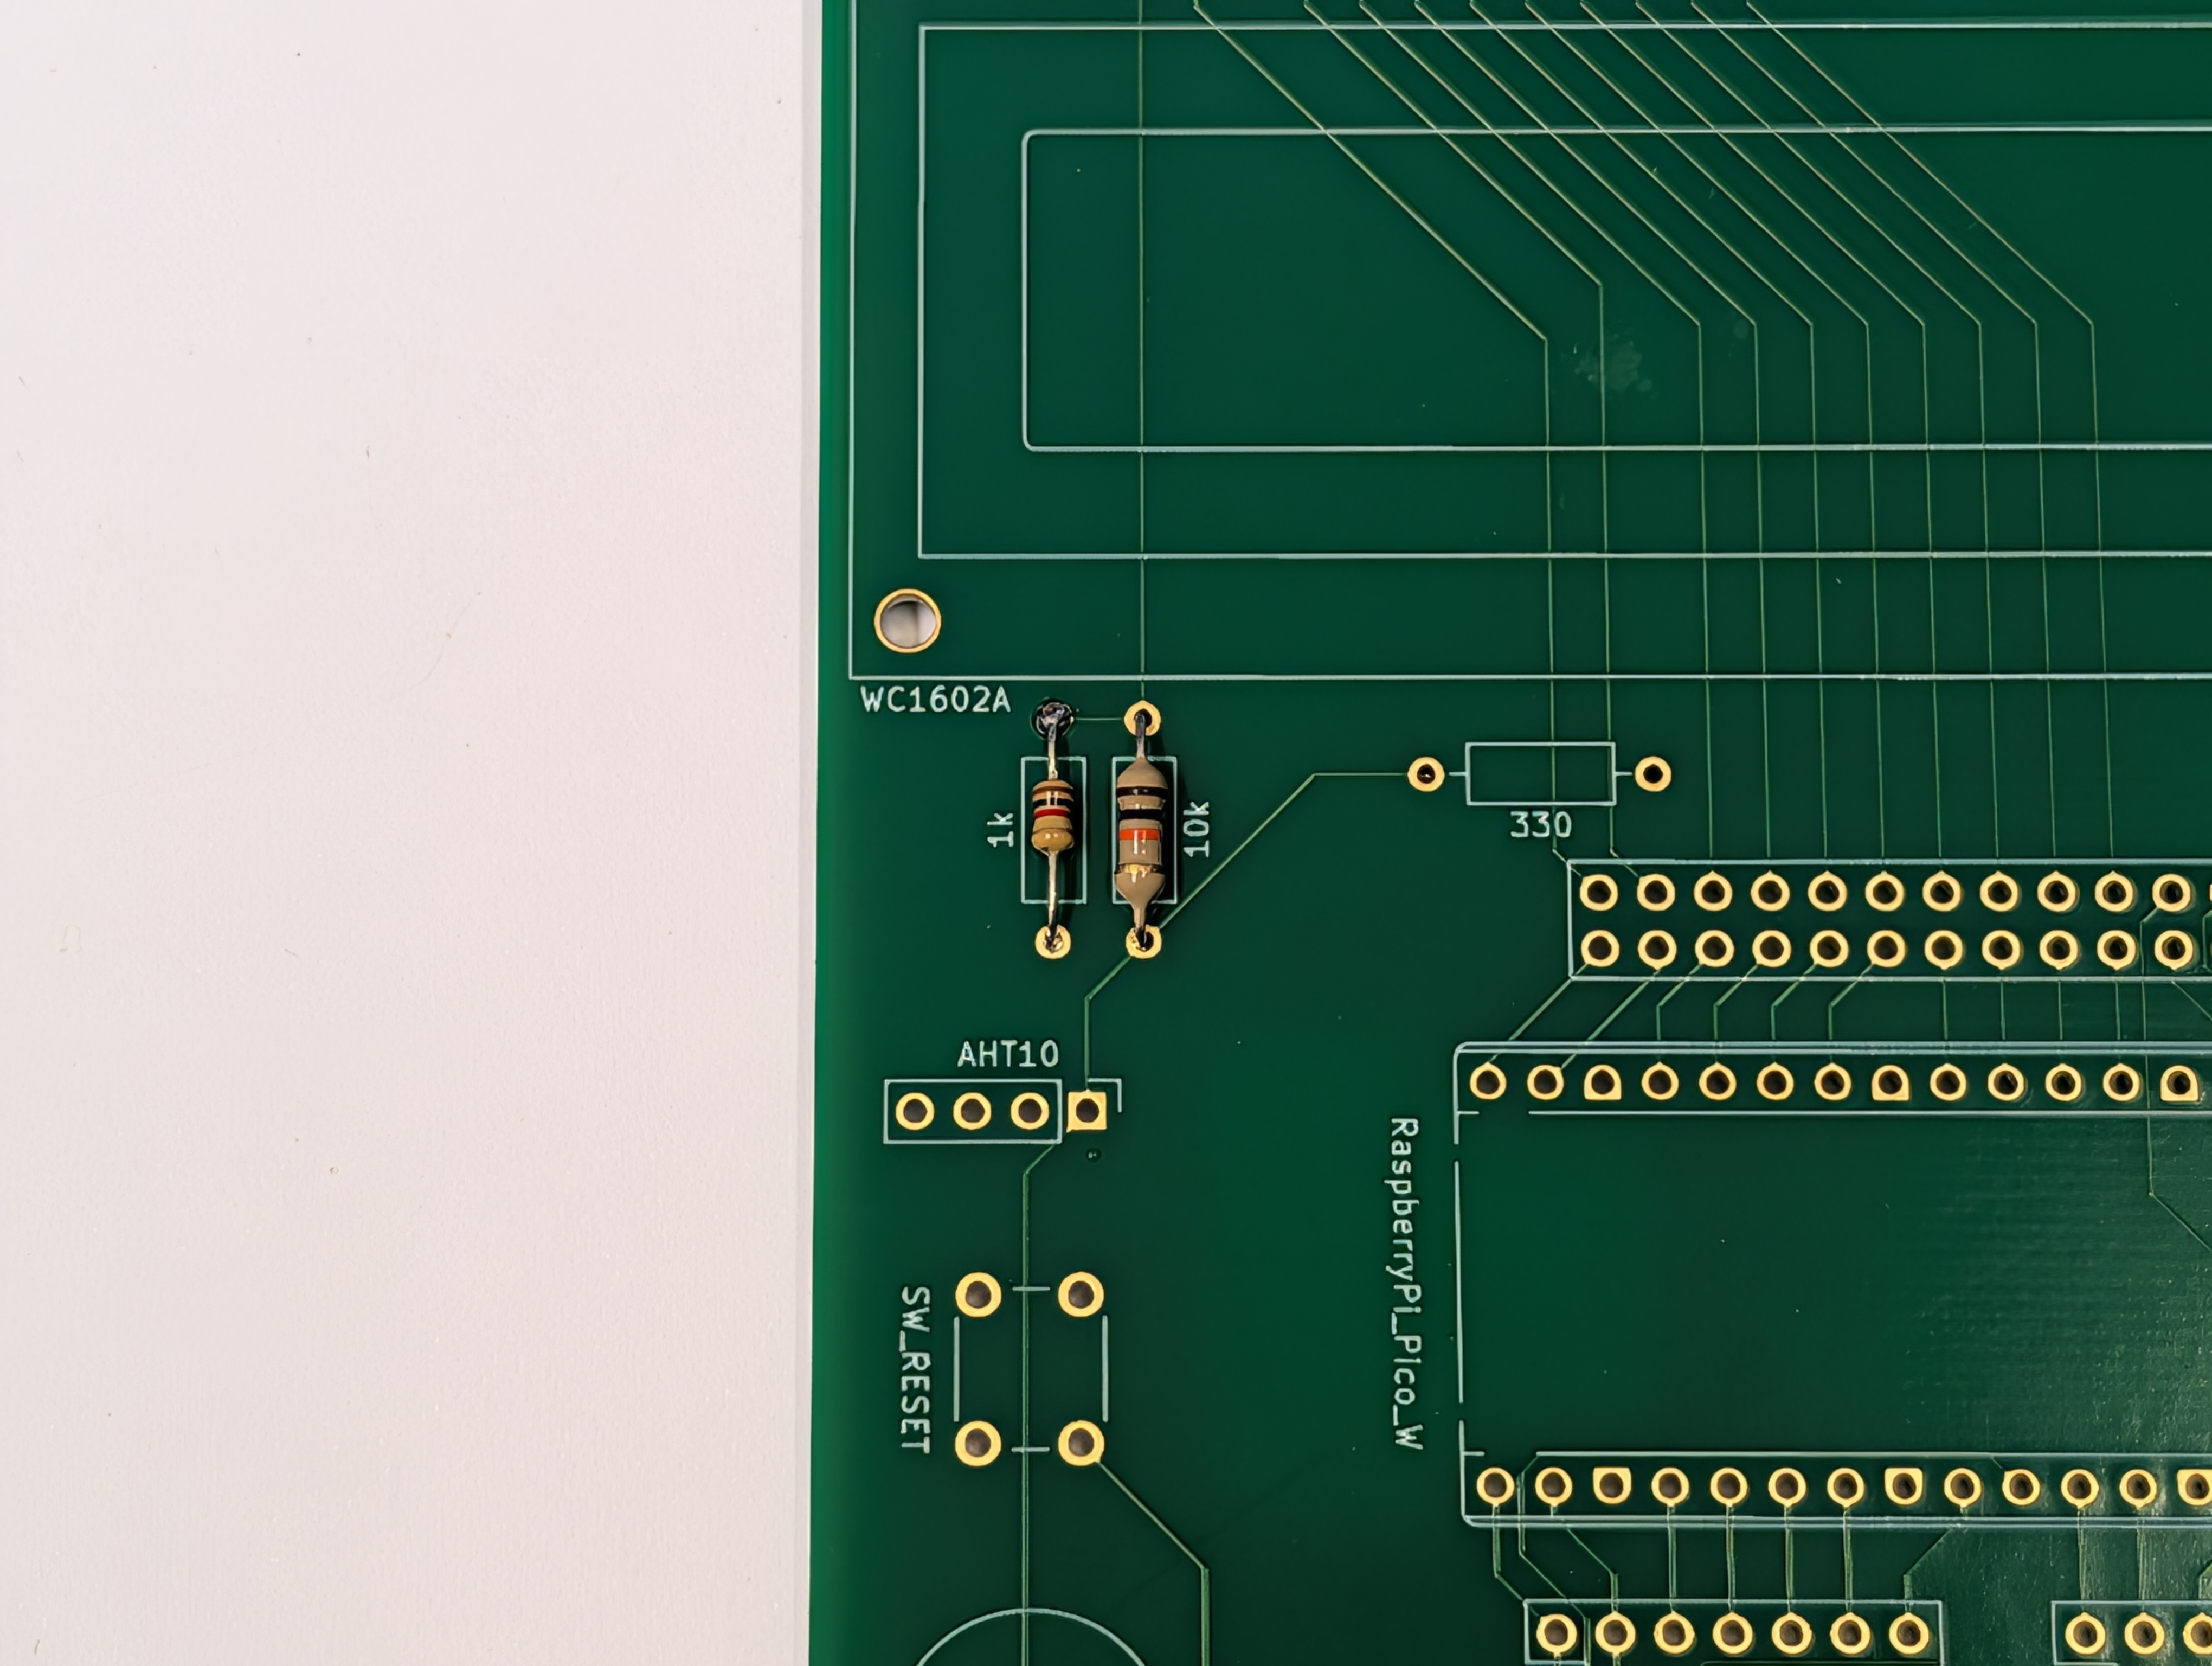
\includegraphics[width=0.75\textwidth]{pictures_of_construction/instruction_step_32.jpg}
\end{figure}

For the 10 k$\Omega$ resistor: form, place, solder one leg, correct, solder fully, and clip flush.

\subsubsection*{330 $\Omega$ resistors}

The 330 $\Omega$ resistors have stripes as markings (Orange | Orange | Black | Black | Brown).

\begin{figure}[H]
    \centering
    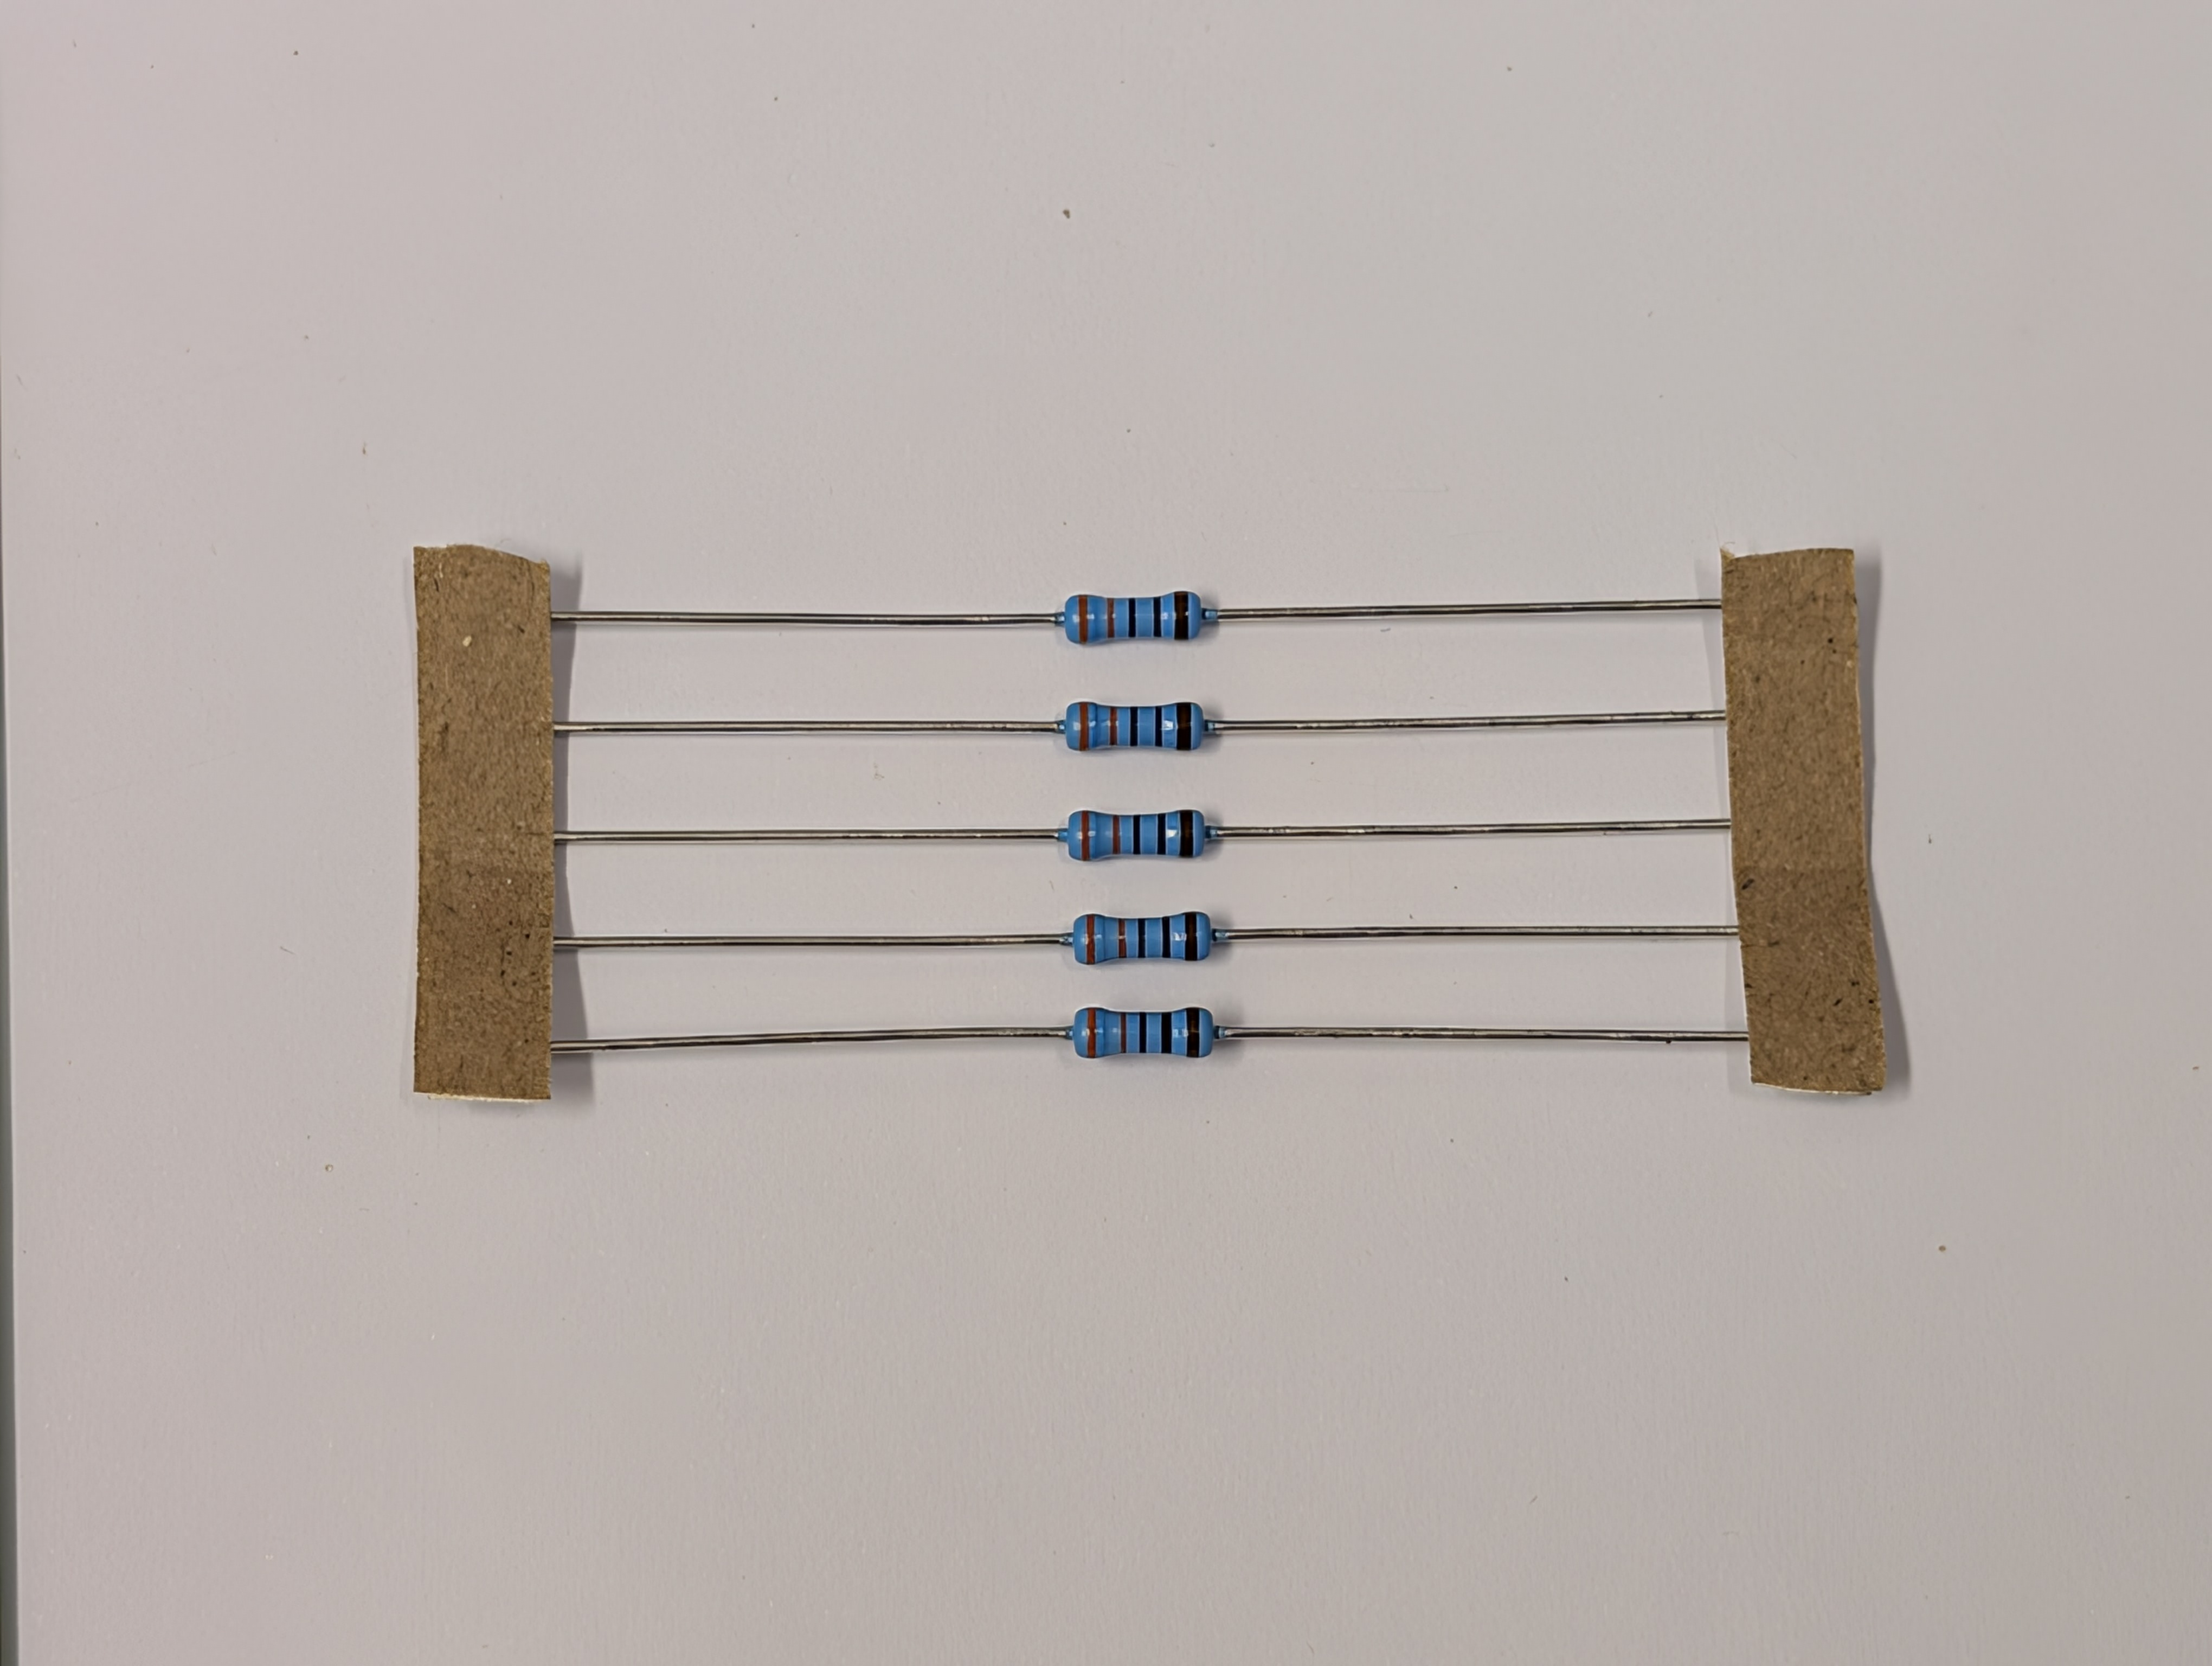
\includegraphics[width=0.75\textwidth]{pictures_of_construction/instruction_step_33.jpg}
\end{figure}

\begin{figure}[H]
    \centering
    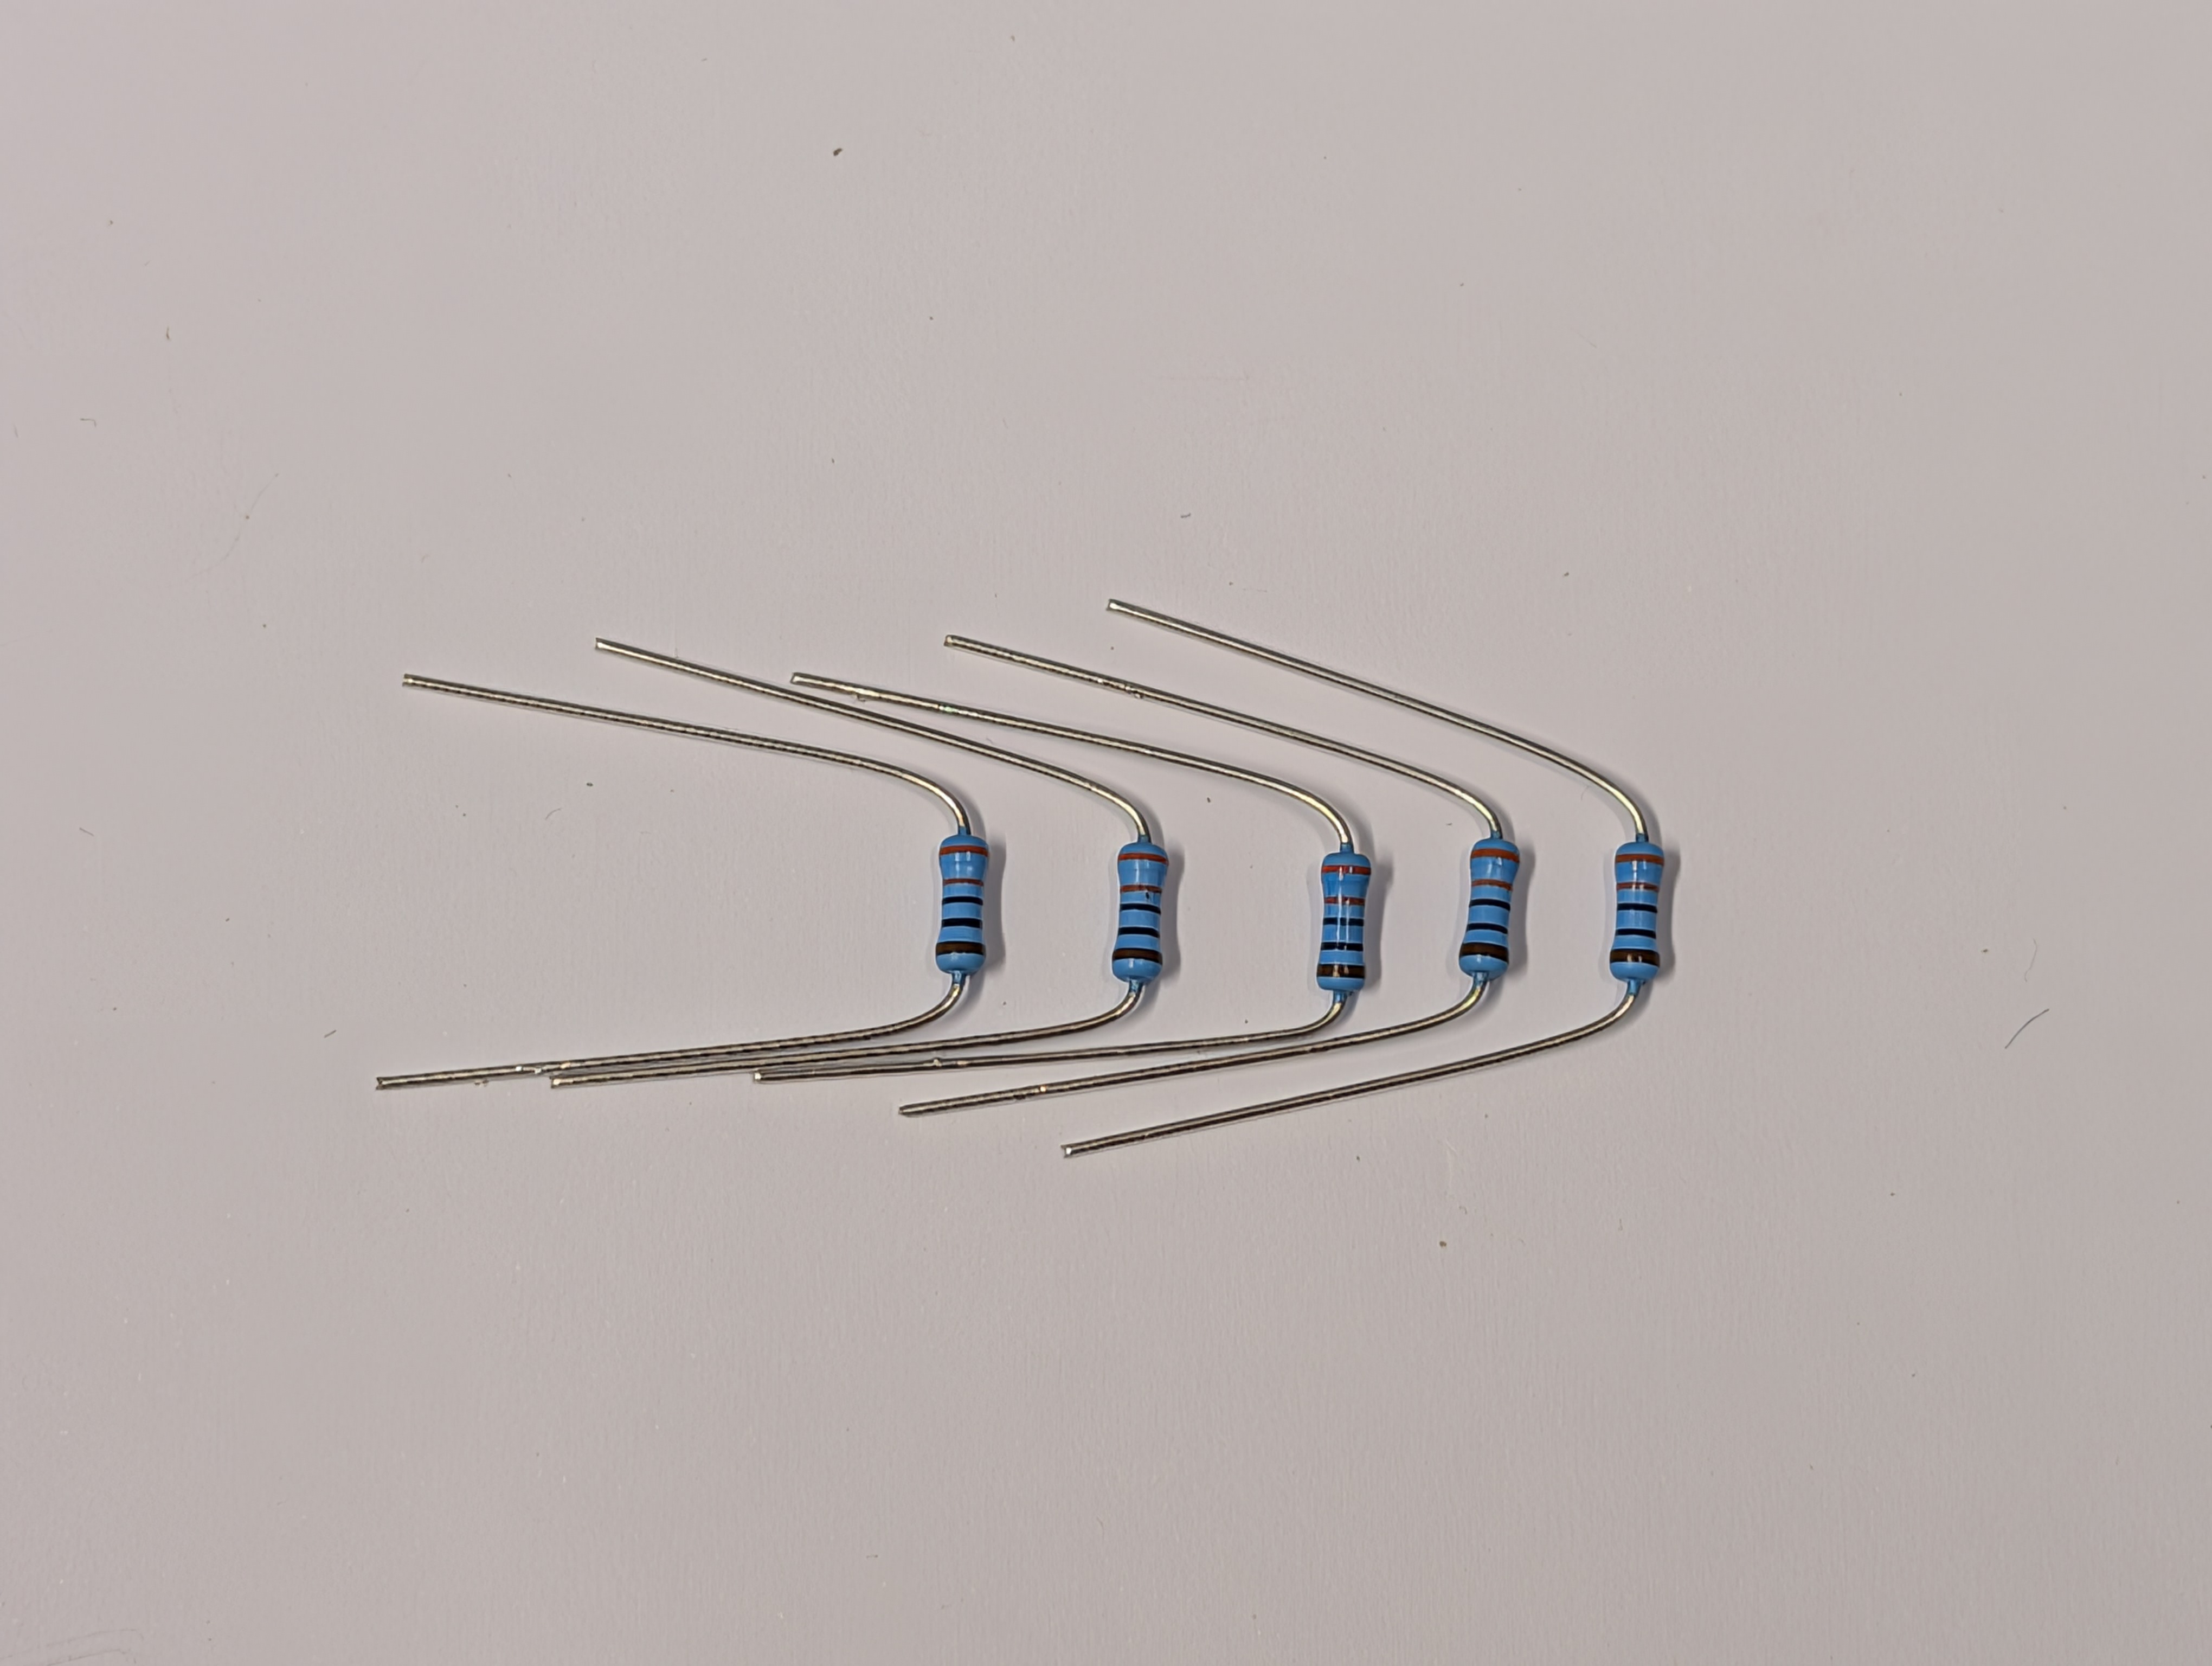
\includegraphics[width=0.75\textwidth]{pictures_of_construction/instruction_step_34.jpg}
\end{figure}

\begin{figure}[H]
    \centering
    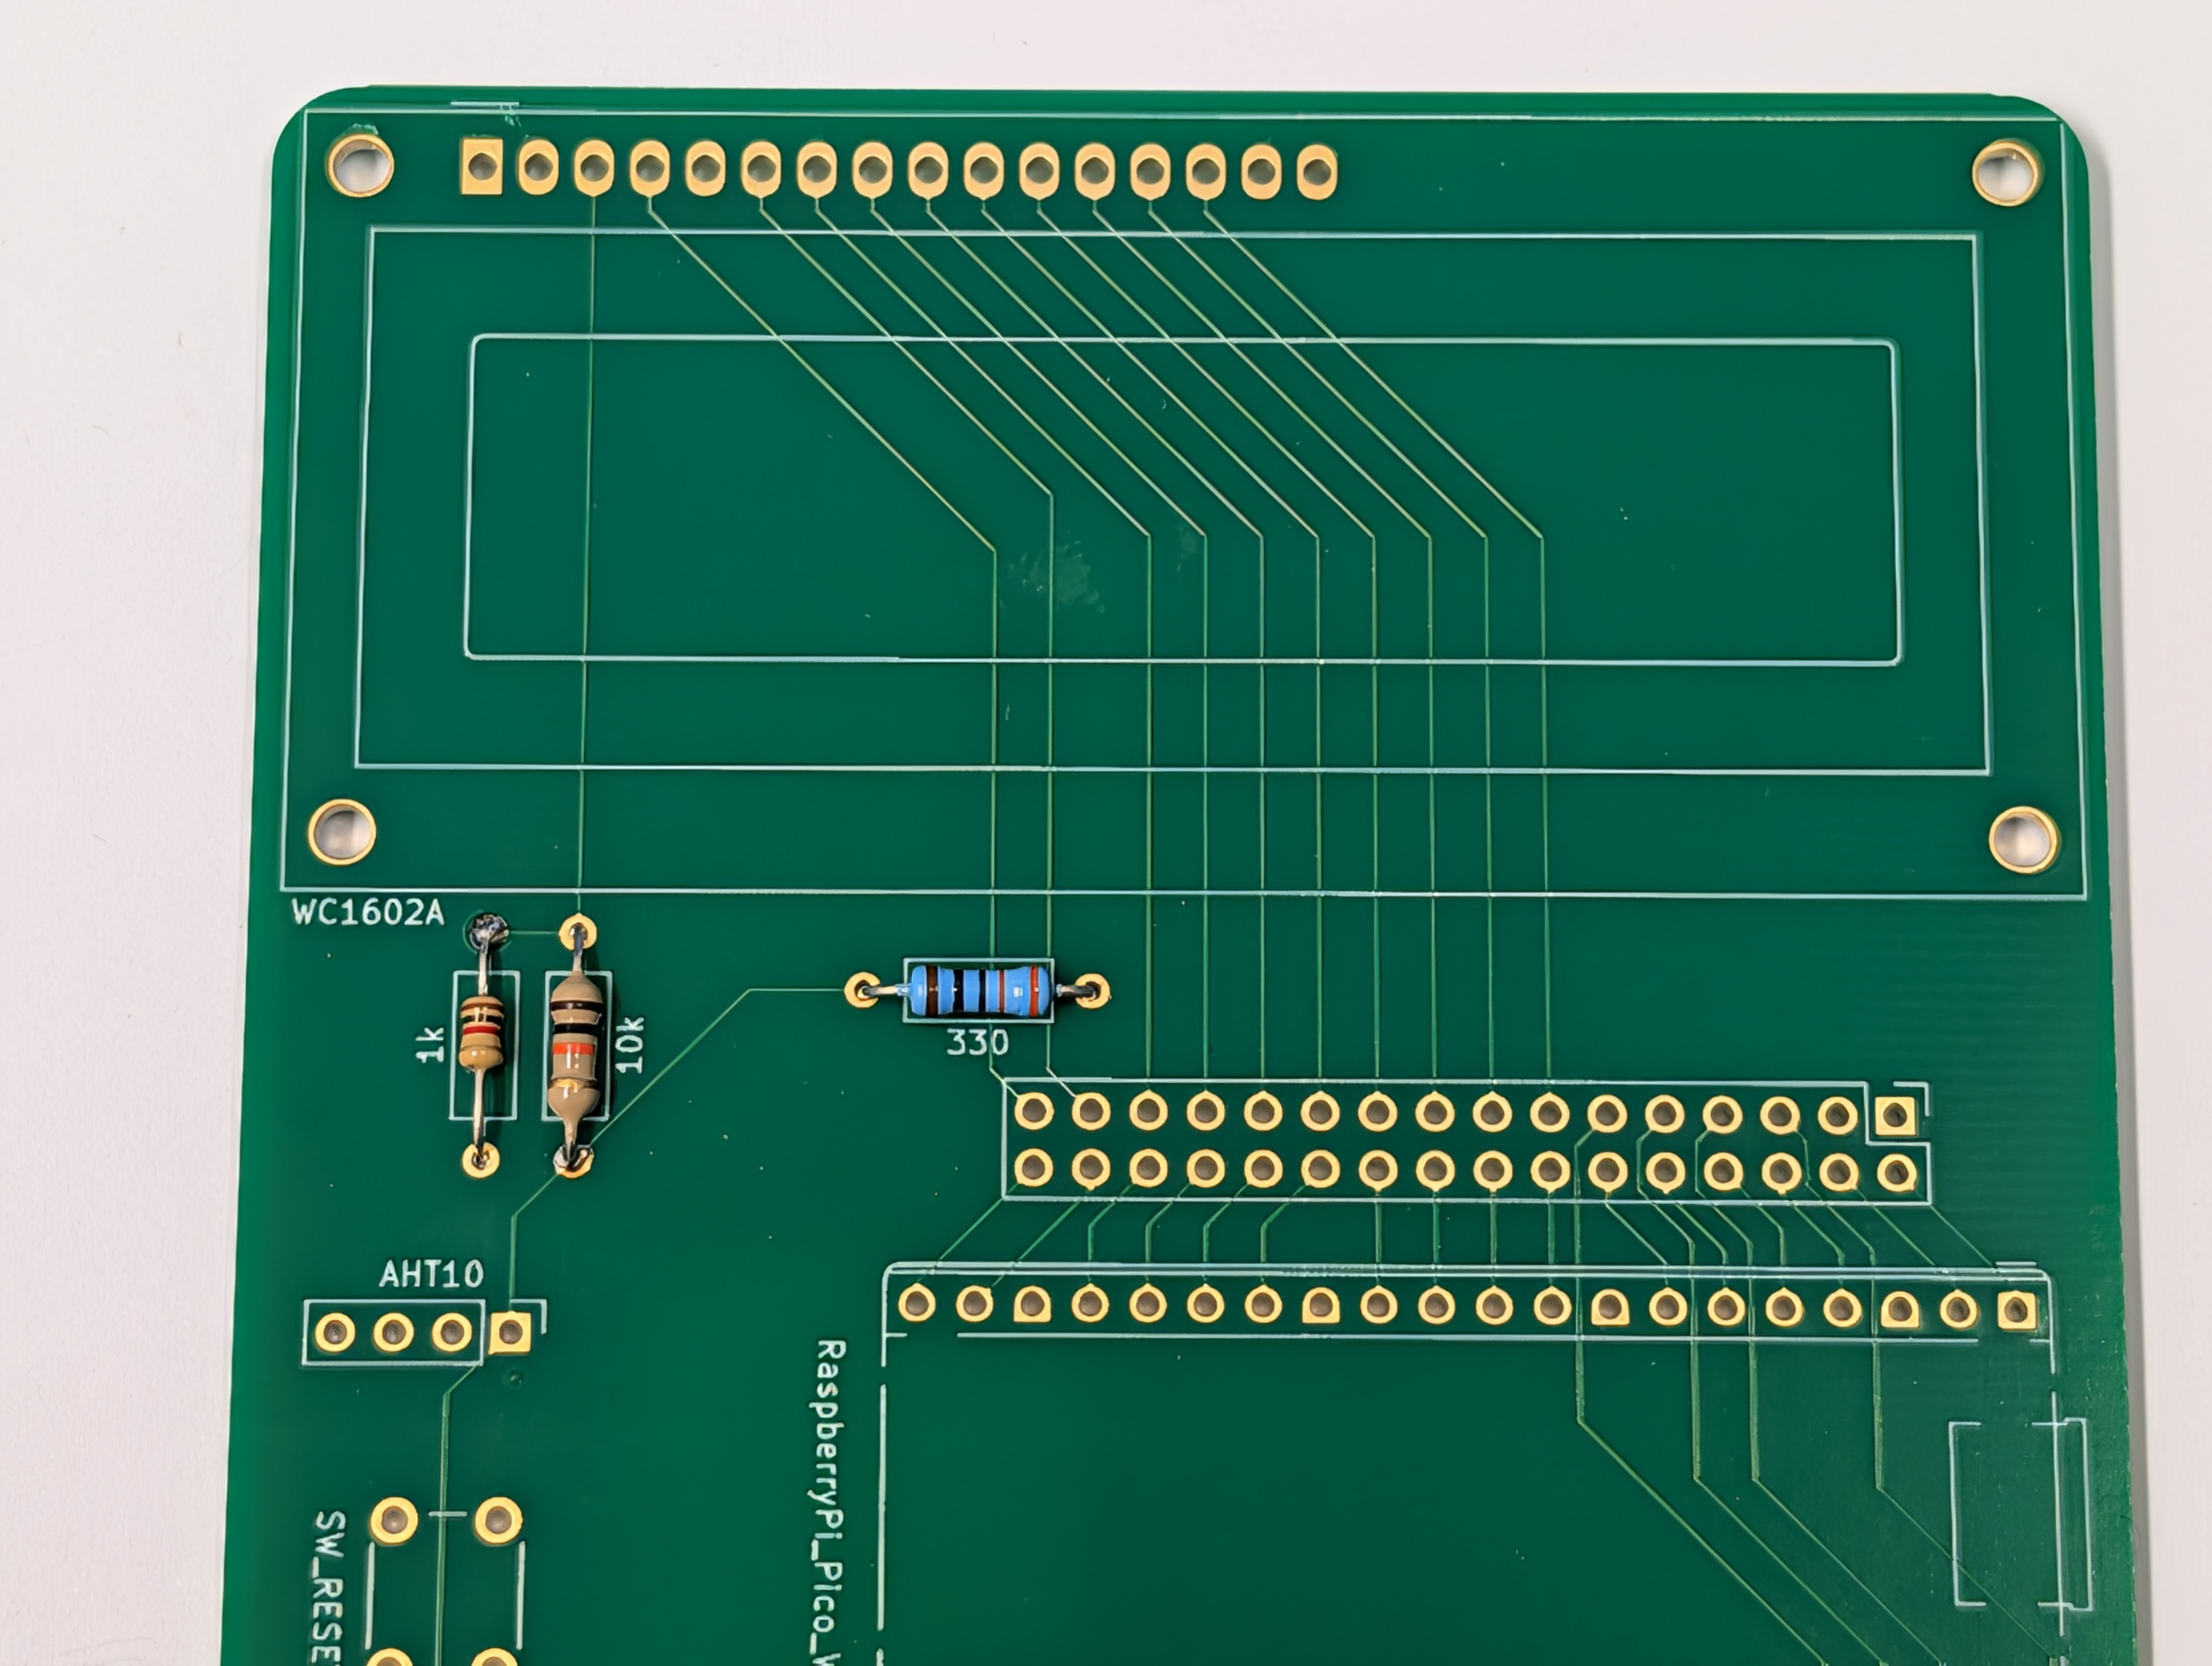
\includegraphics[width=0.75\textwidth]{pictures_of_construction/instruction_step_35.jpg}
\end{figure}

\begin{figure}[H]
    \centering
    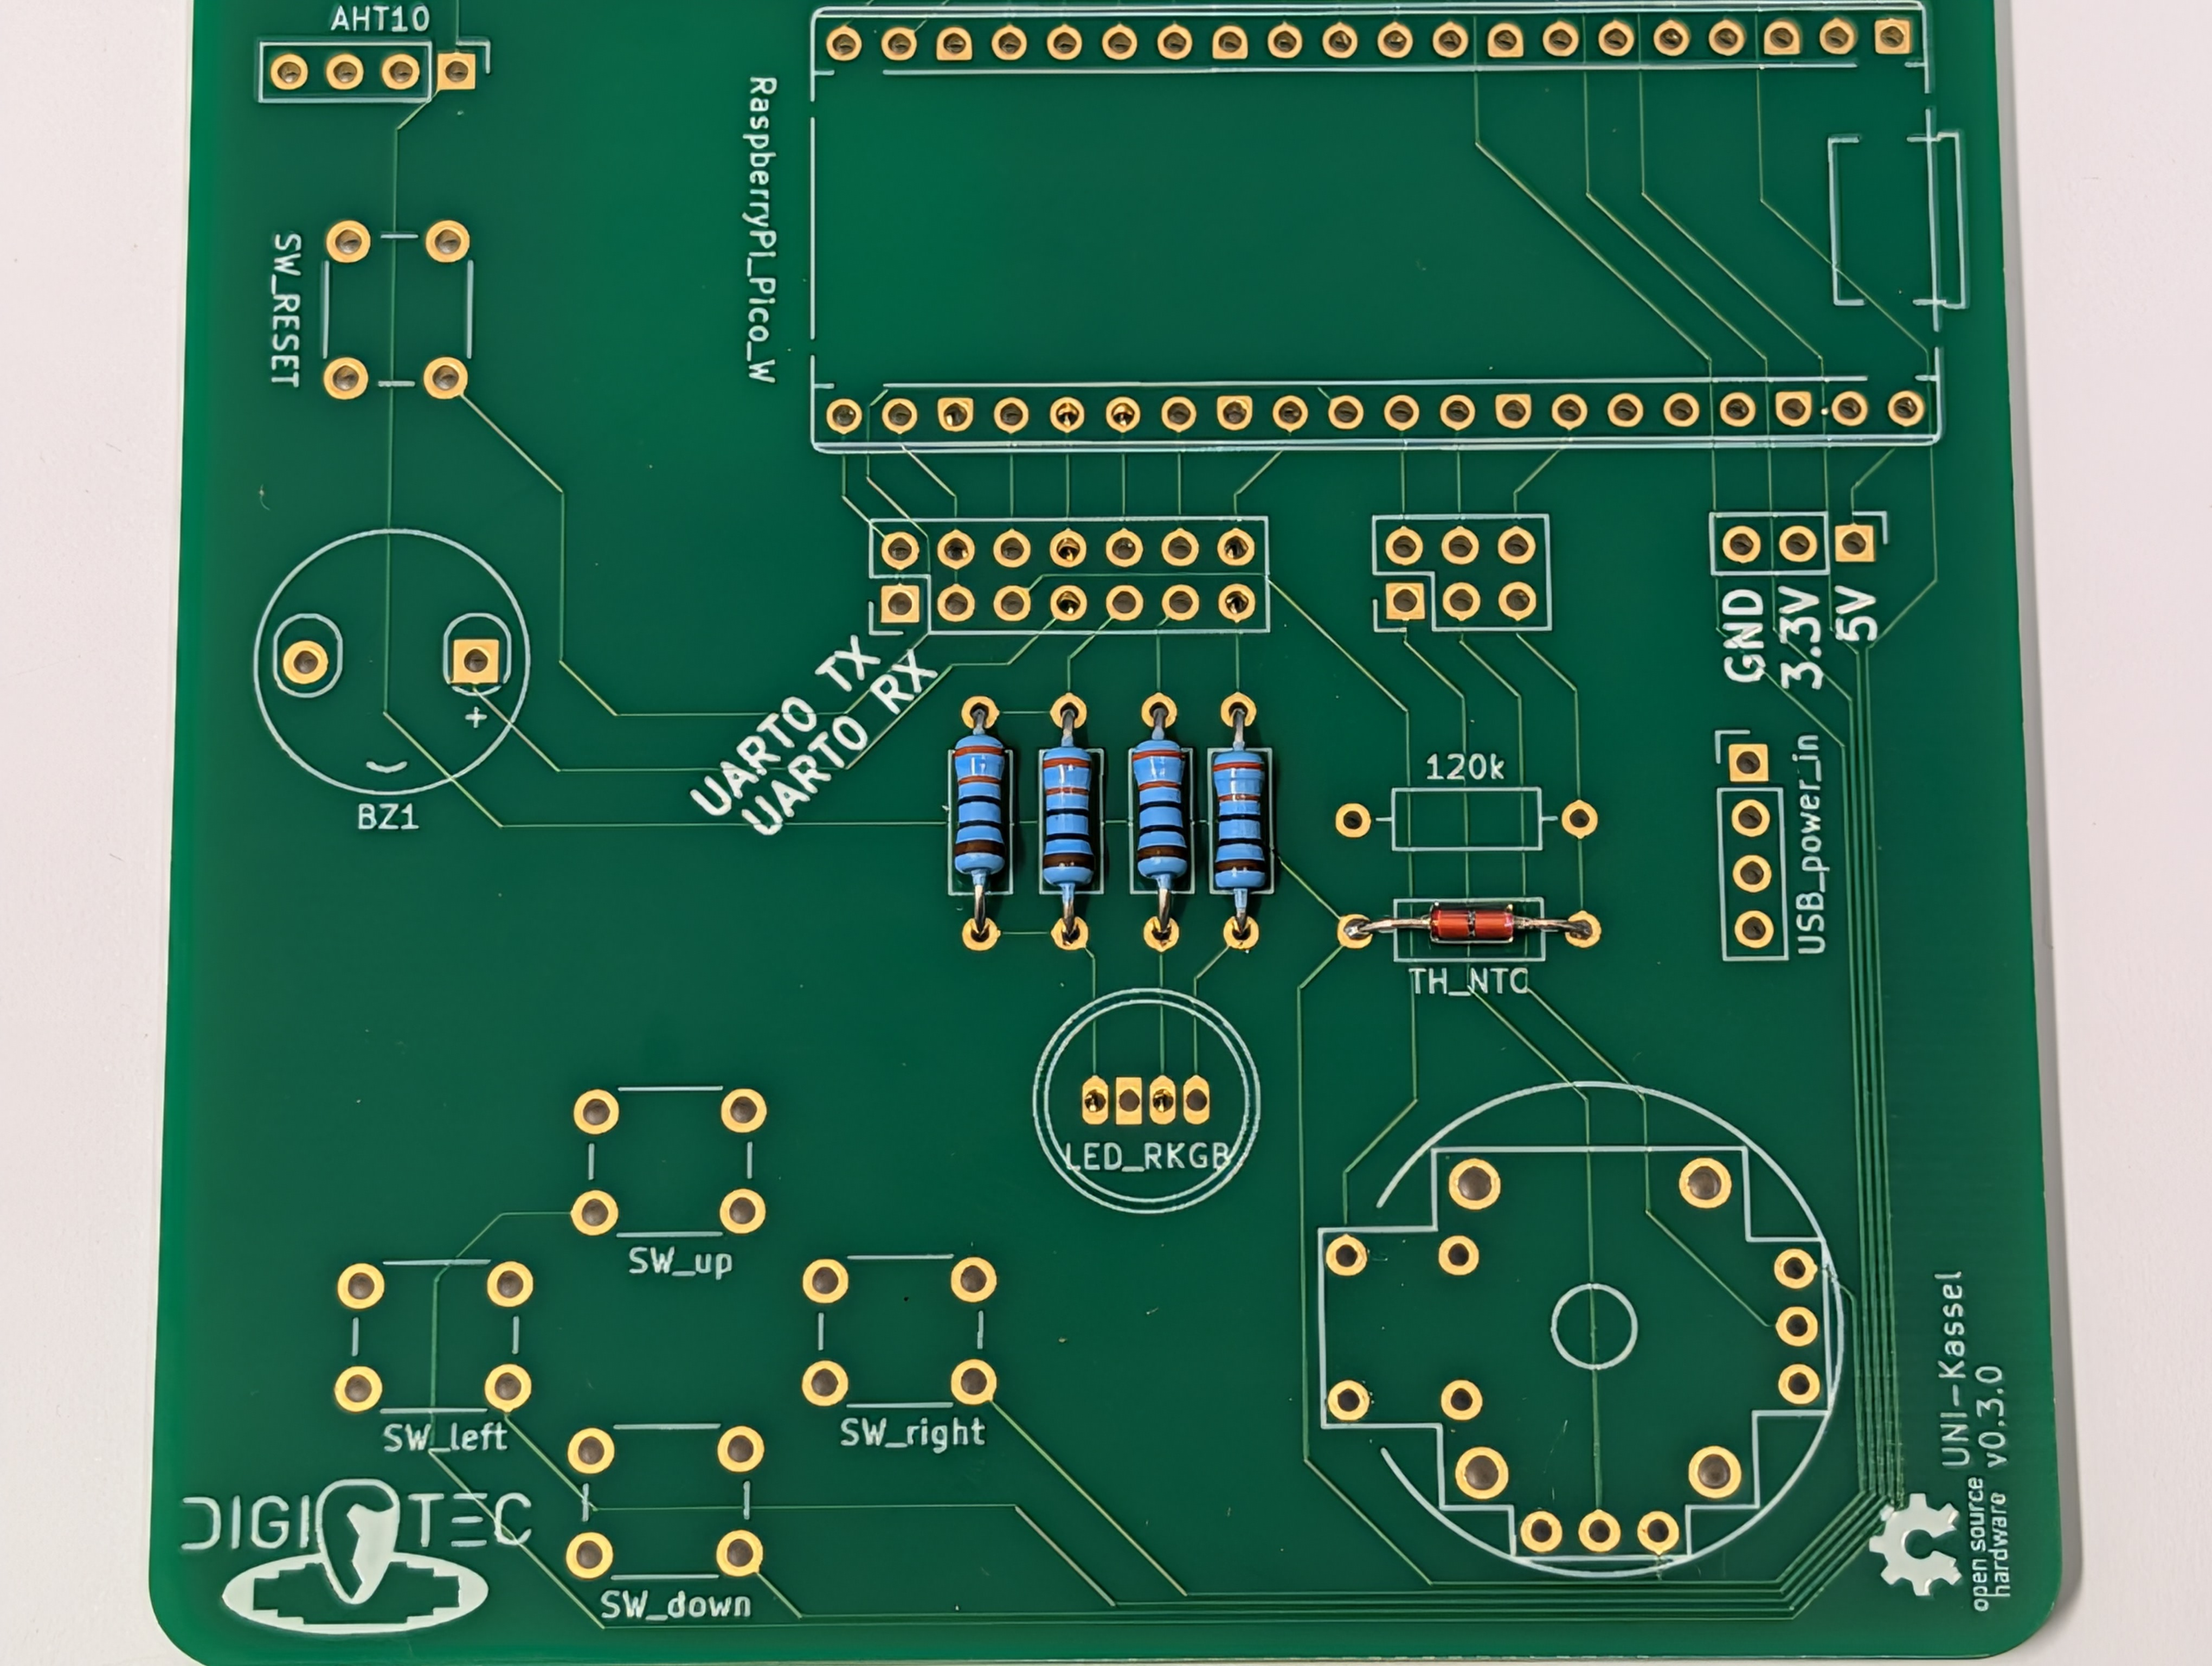
\includegraphics[width=0.75\textwidth]{pictures_of_construction/instruction_step_36.jpg}
\end{figure}

For the 330 $\Omega$ resistors: form, place, solder one leg, correct, solder fully, and clip flush.

\subsubsection*{120 k$\Omega$ resistor}

The 120 k$\Omega$ resistor has stripes as markings (Brown | Red | Yellow | Gold).

\begin{figure}[H]
    \centering
    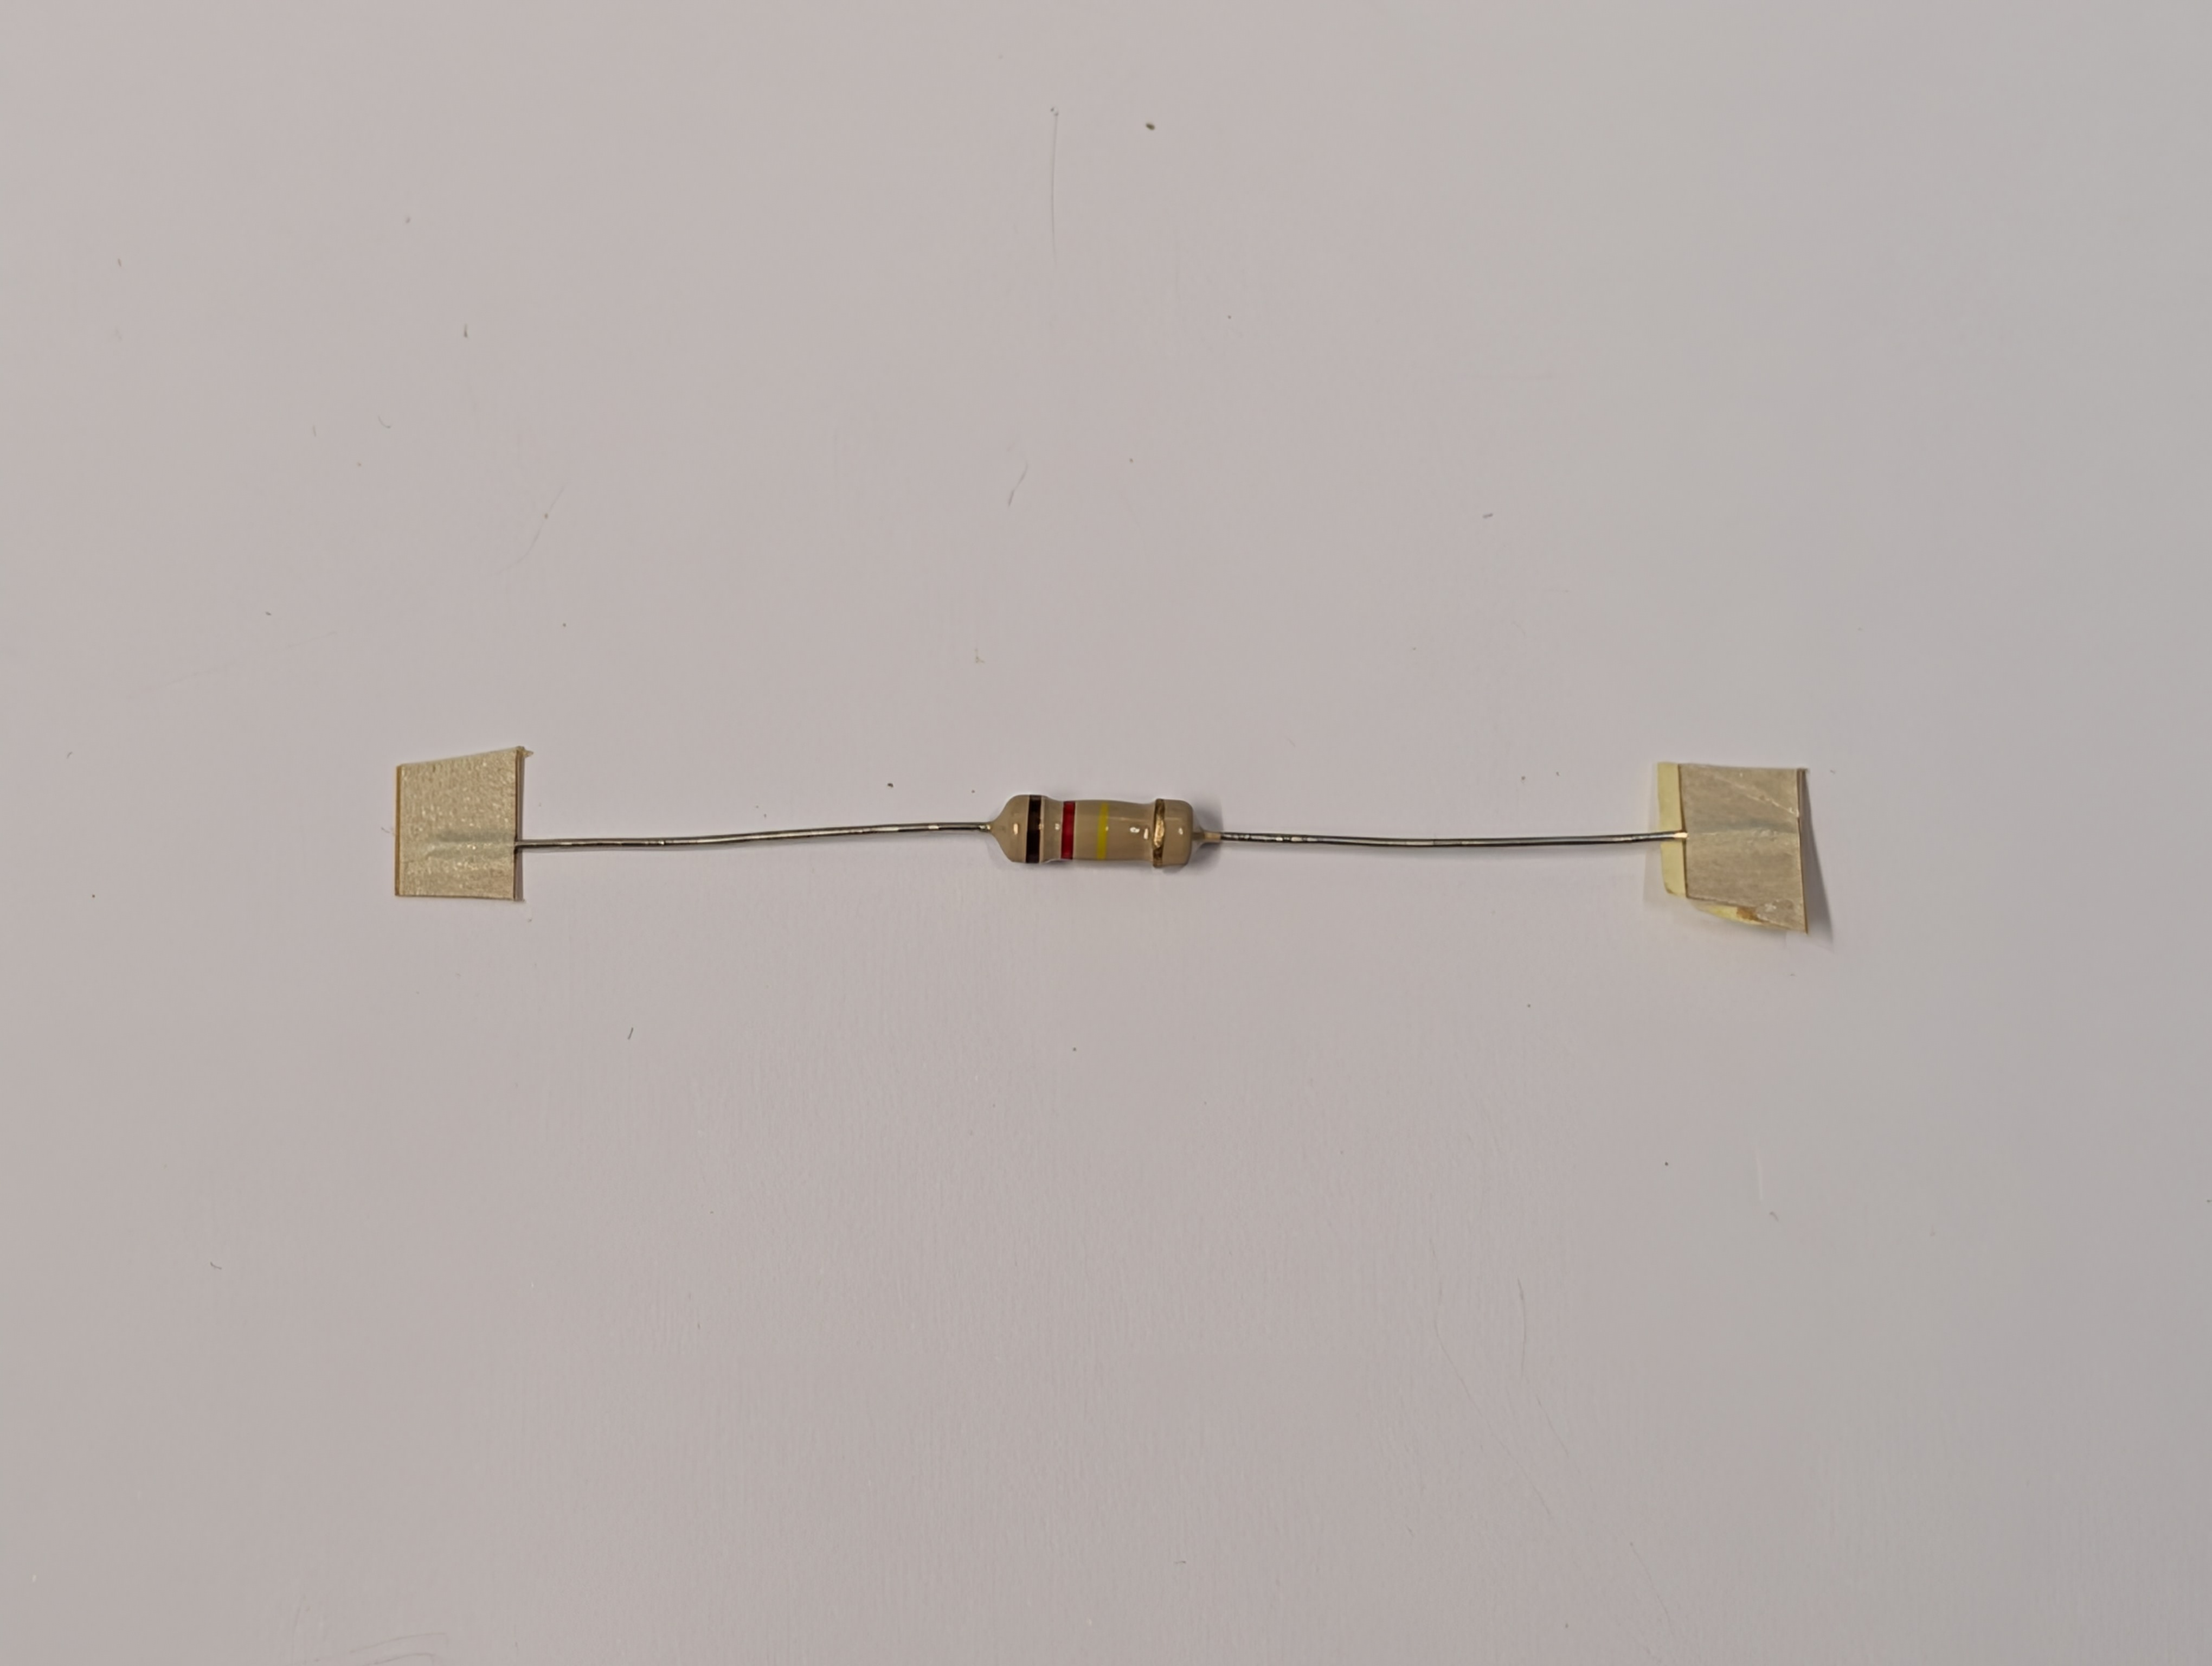
\includegraphics[width=0.75\textwidth]{pictures_of_construction/instruction_step_37.jpg}
\end{figure}

\begin{figure}[H]
    \centering
    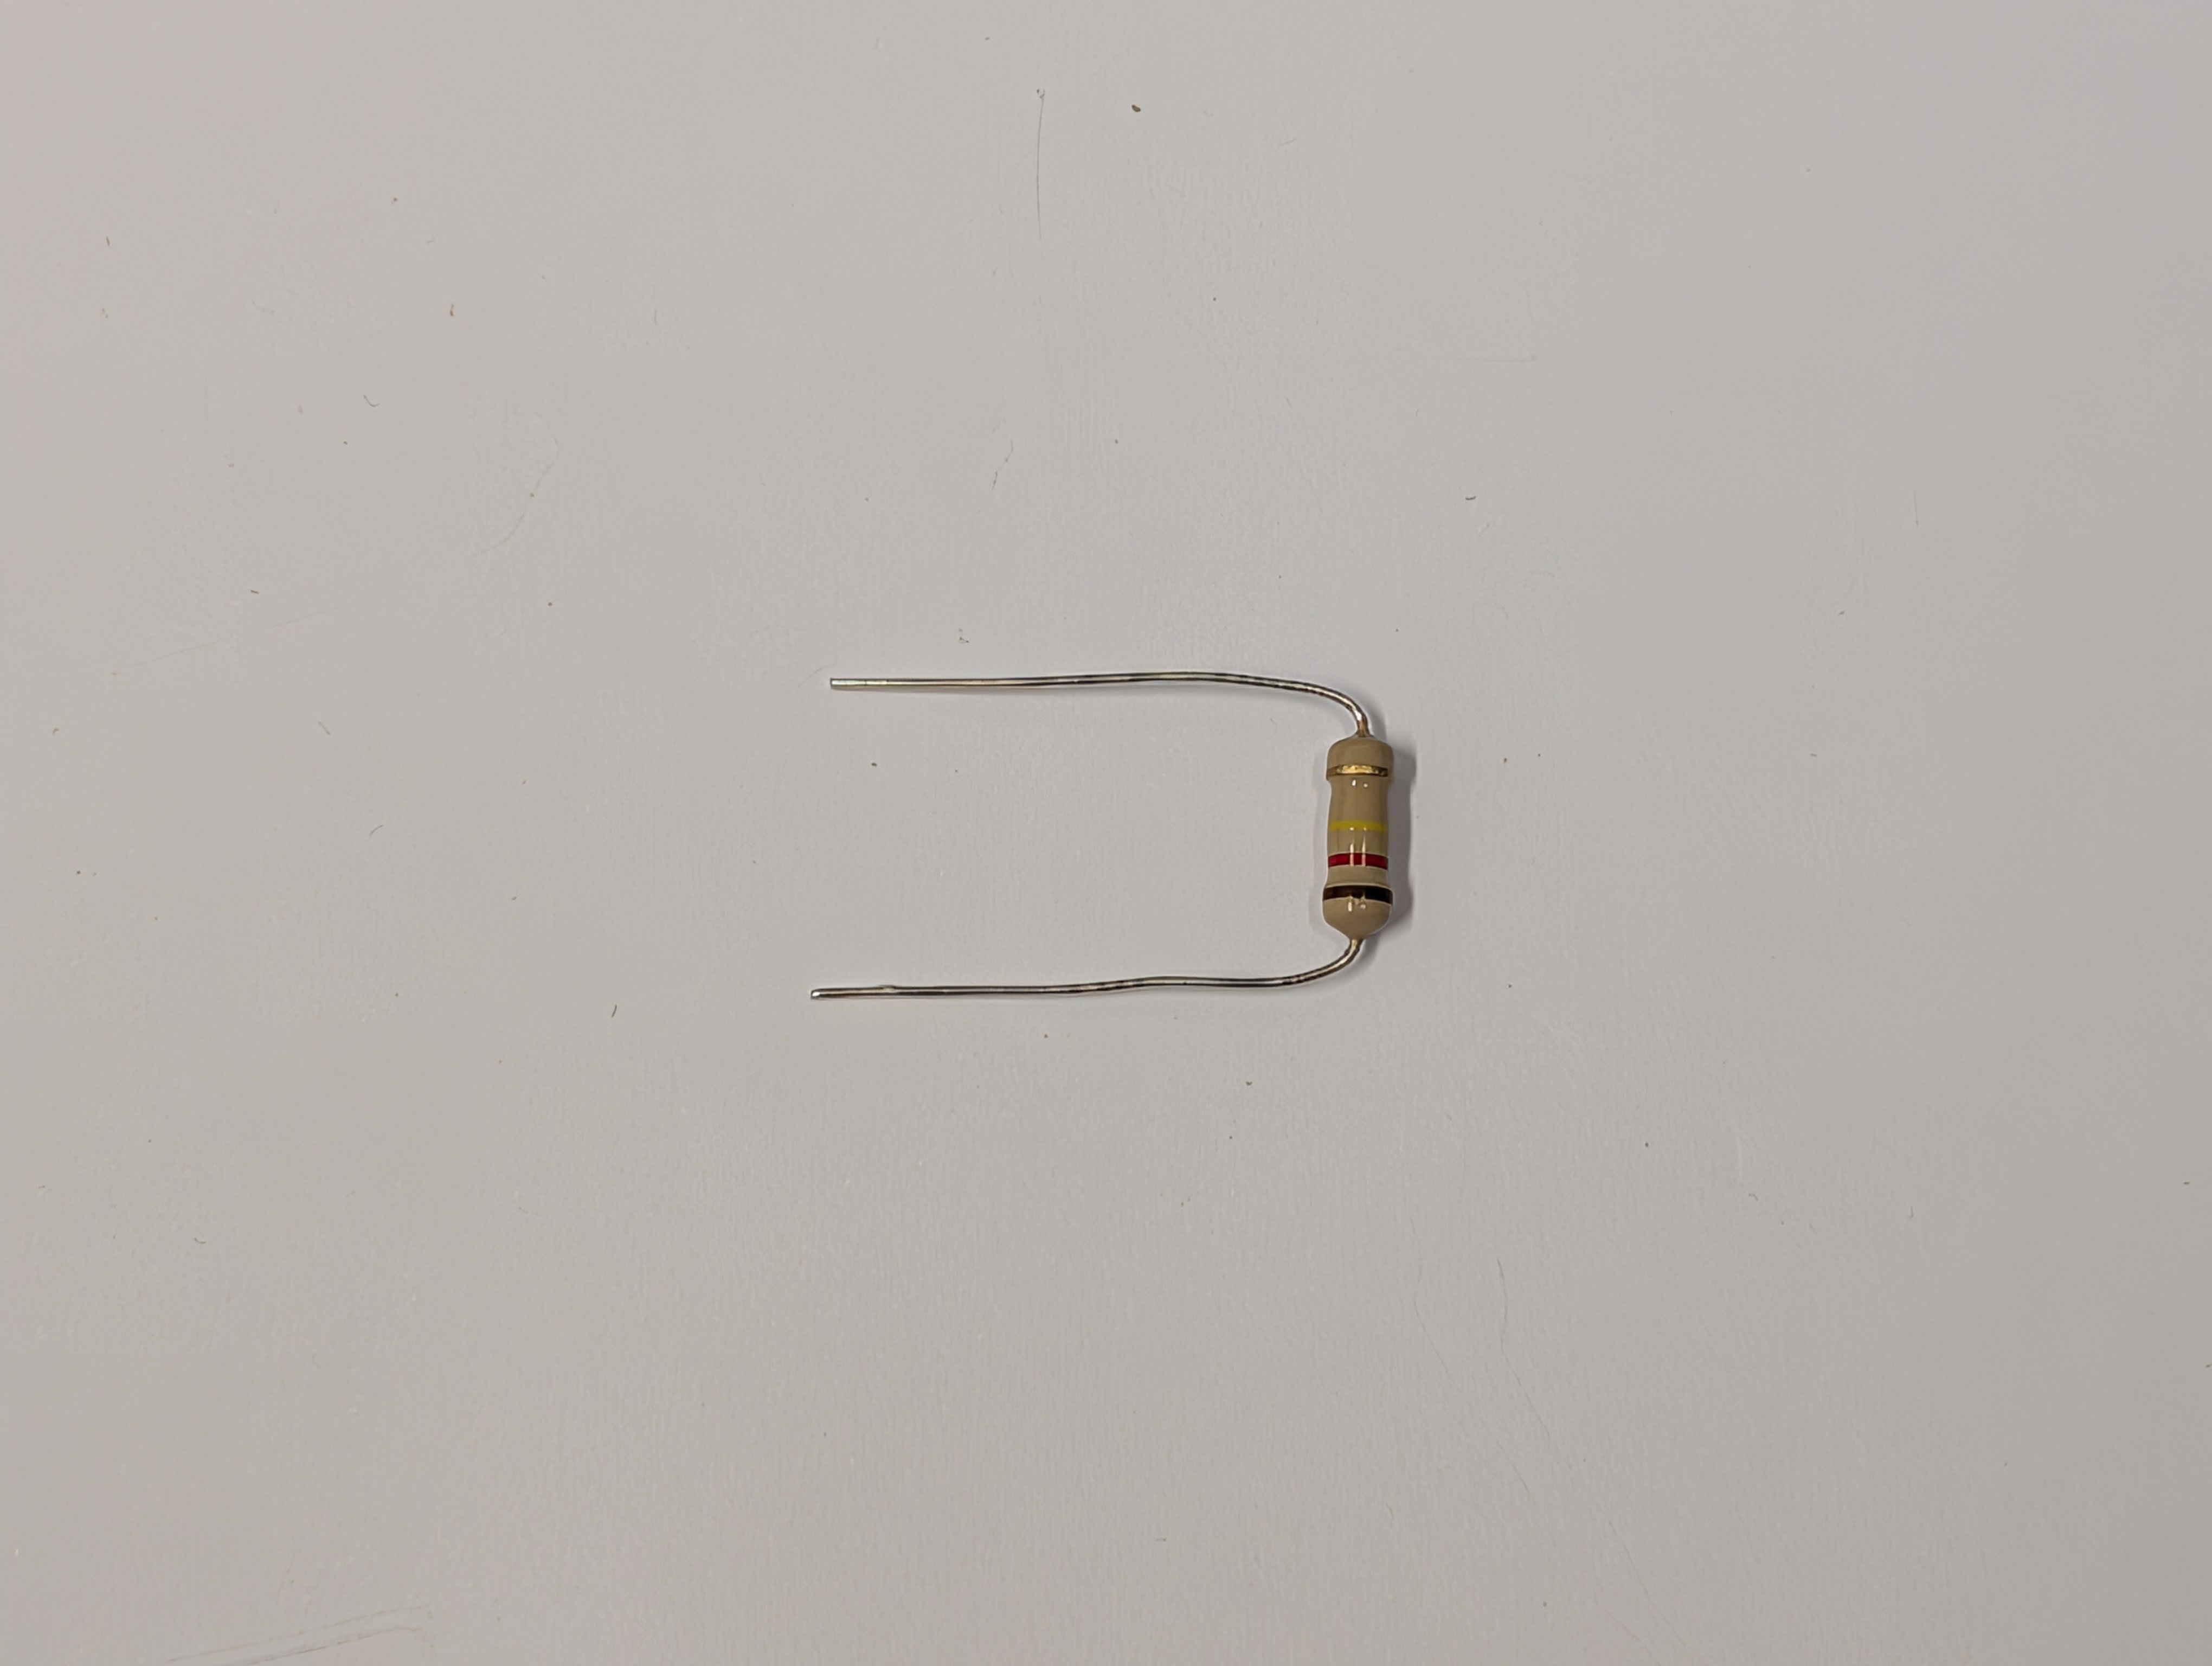
\includegraphics[width=0.75\textwidth]{pictures_of_construction/instruction_step_38.jpg}
\end{figure}

\begin{figure}[H]
    \centering
    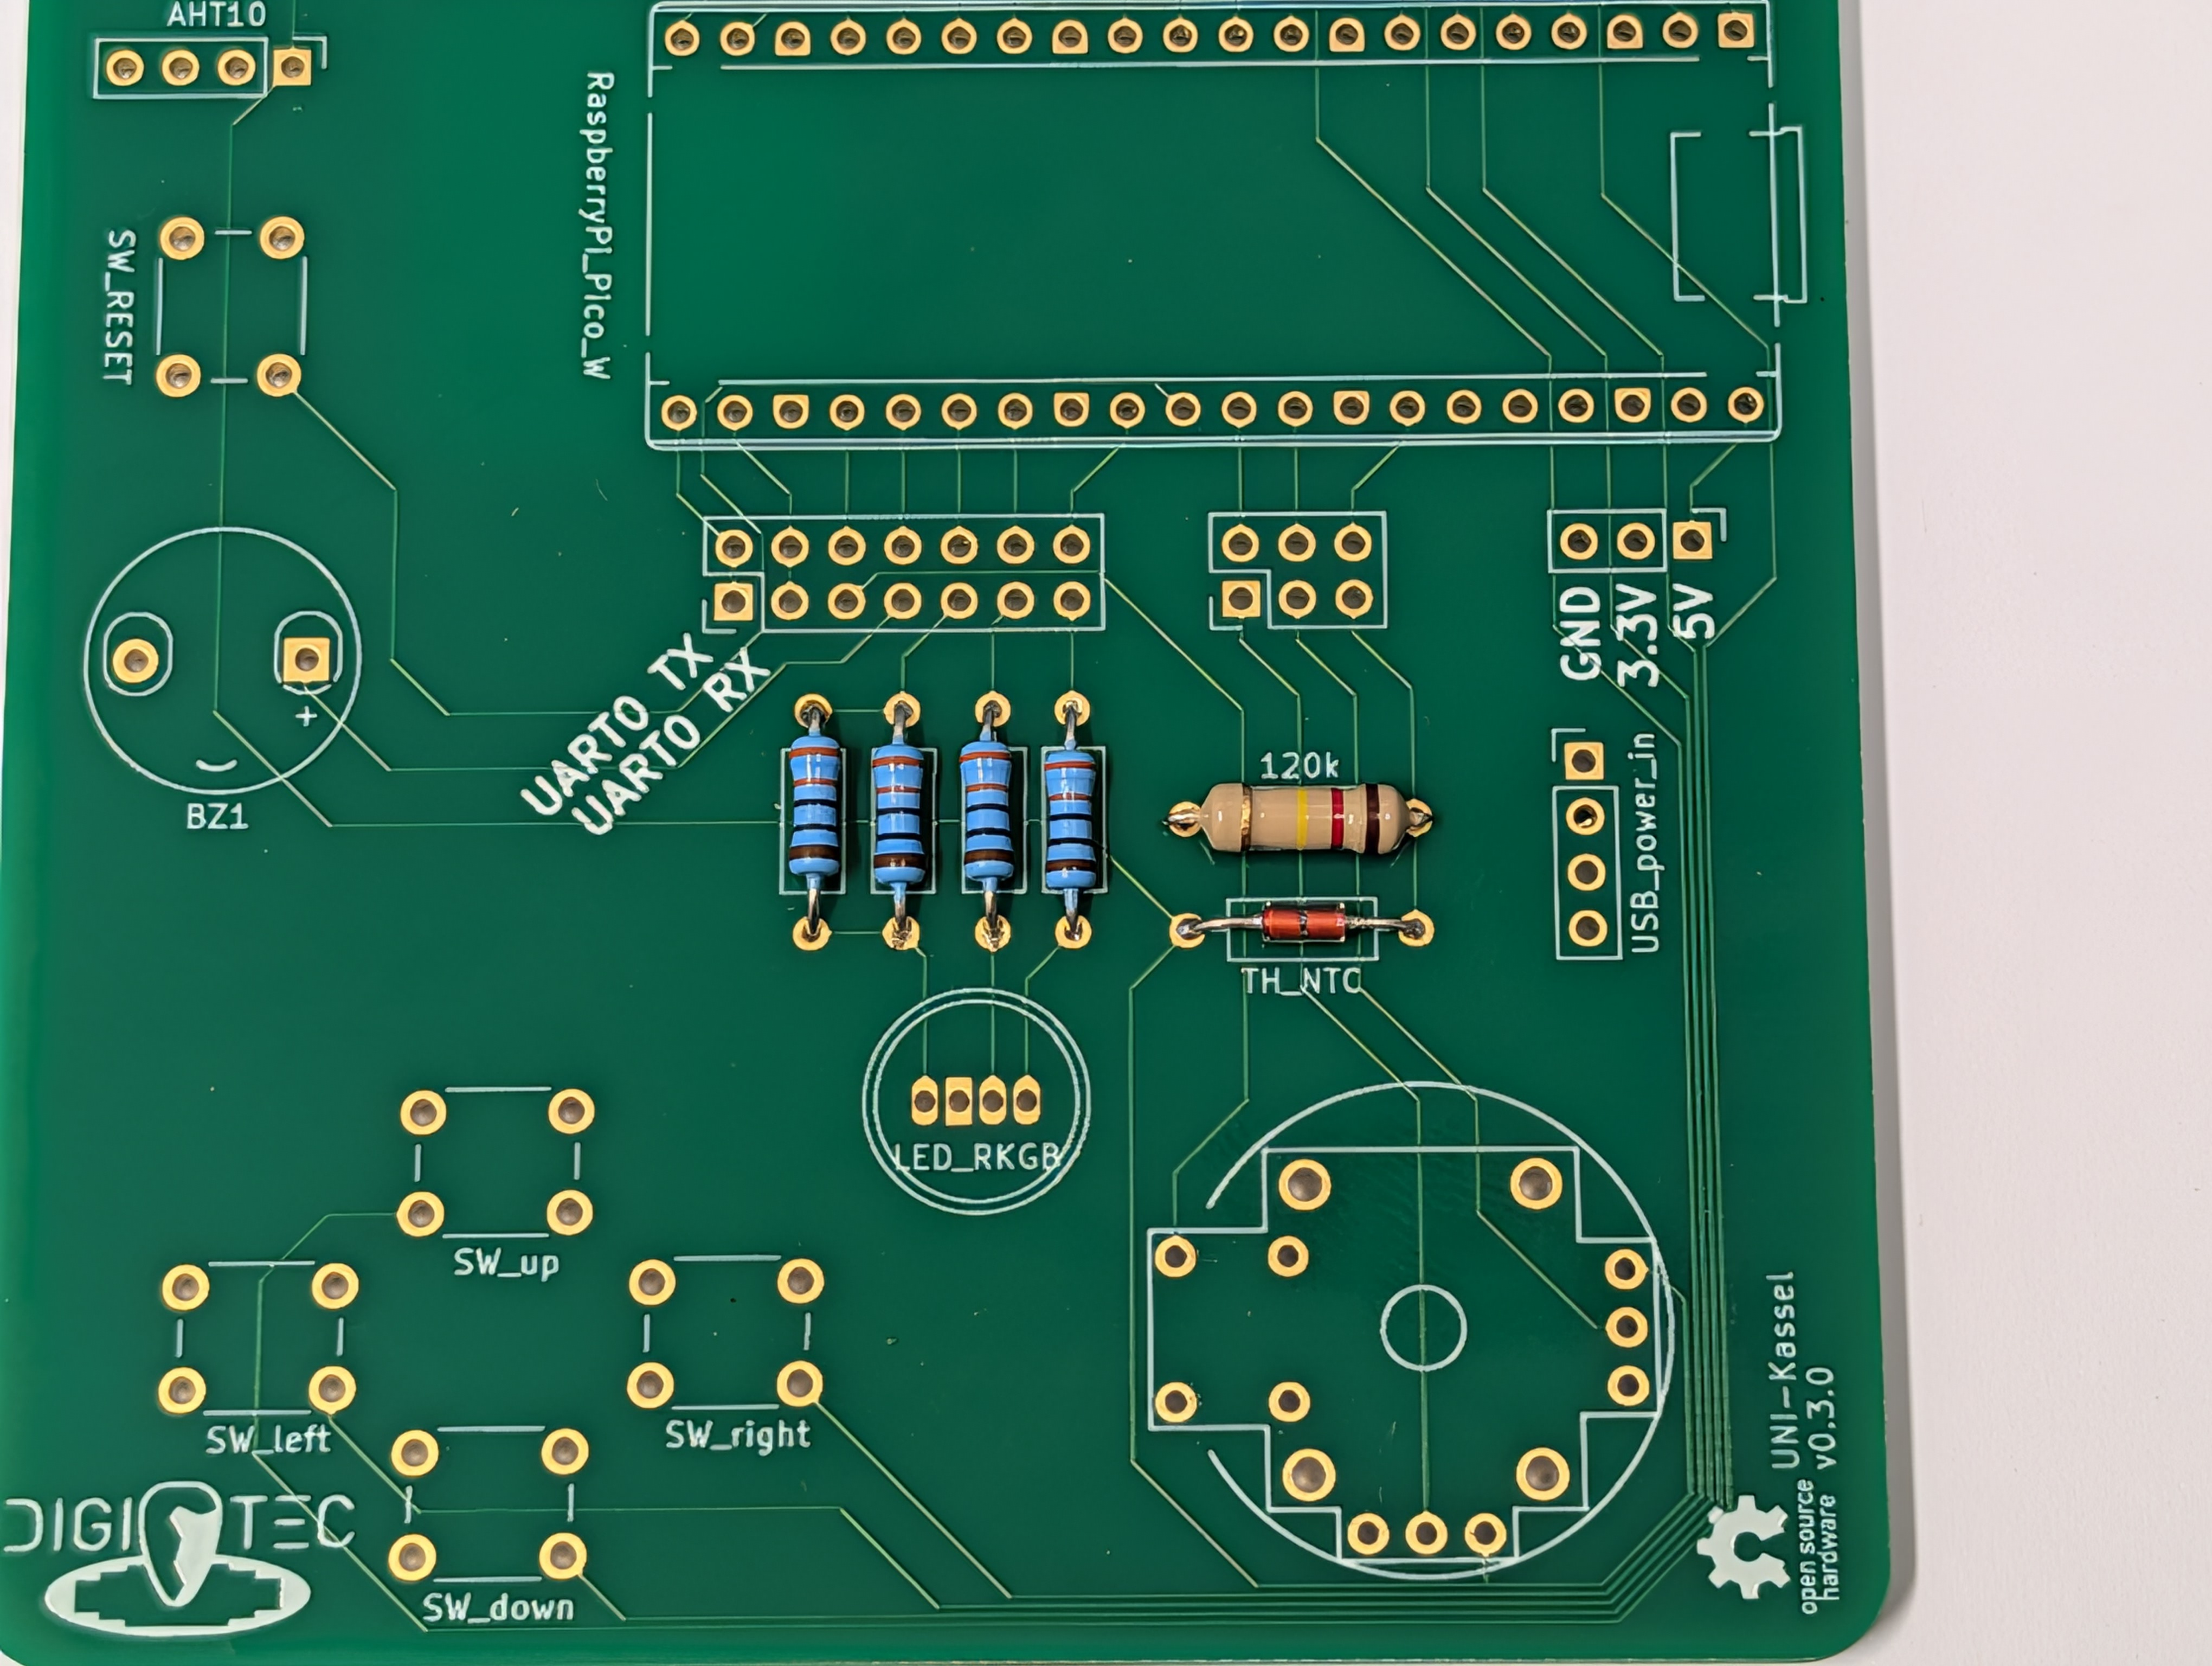
\includegraphics[width=0.75\textwidth]{pictures_of_construction/instruction_step_39.jpg}
\end{figure}

For the 120 k$\Omega$ resistor: form, place, solder one leg, correct, solder fully, and clip flush.

\subsection*{Installation of the buttons}

\begin{figure}[H]
    \centering
    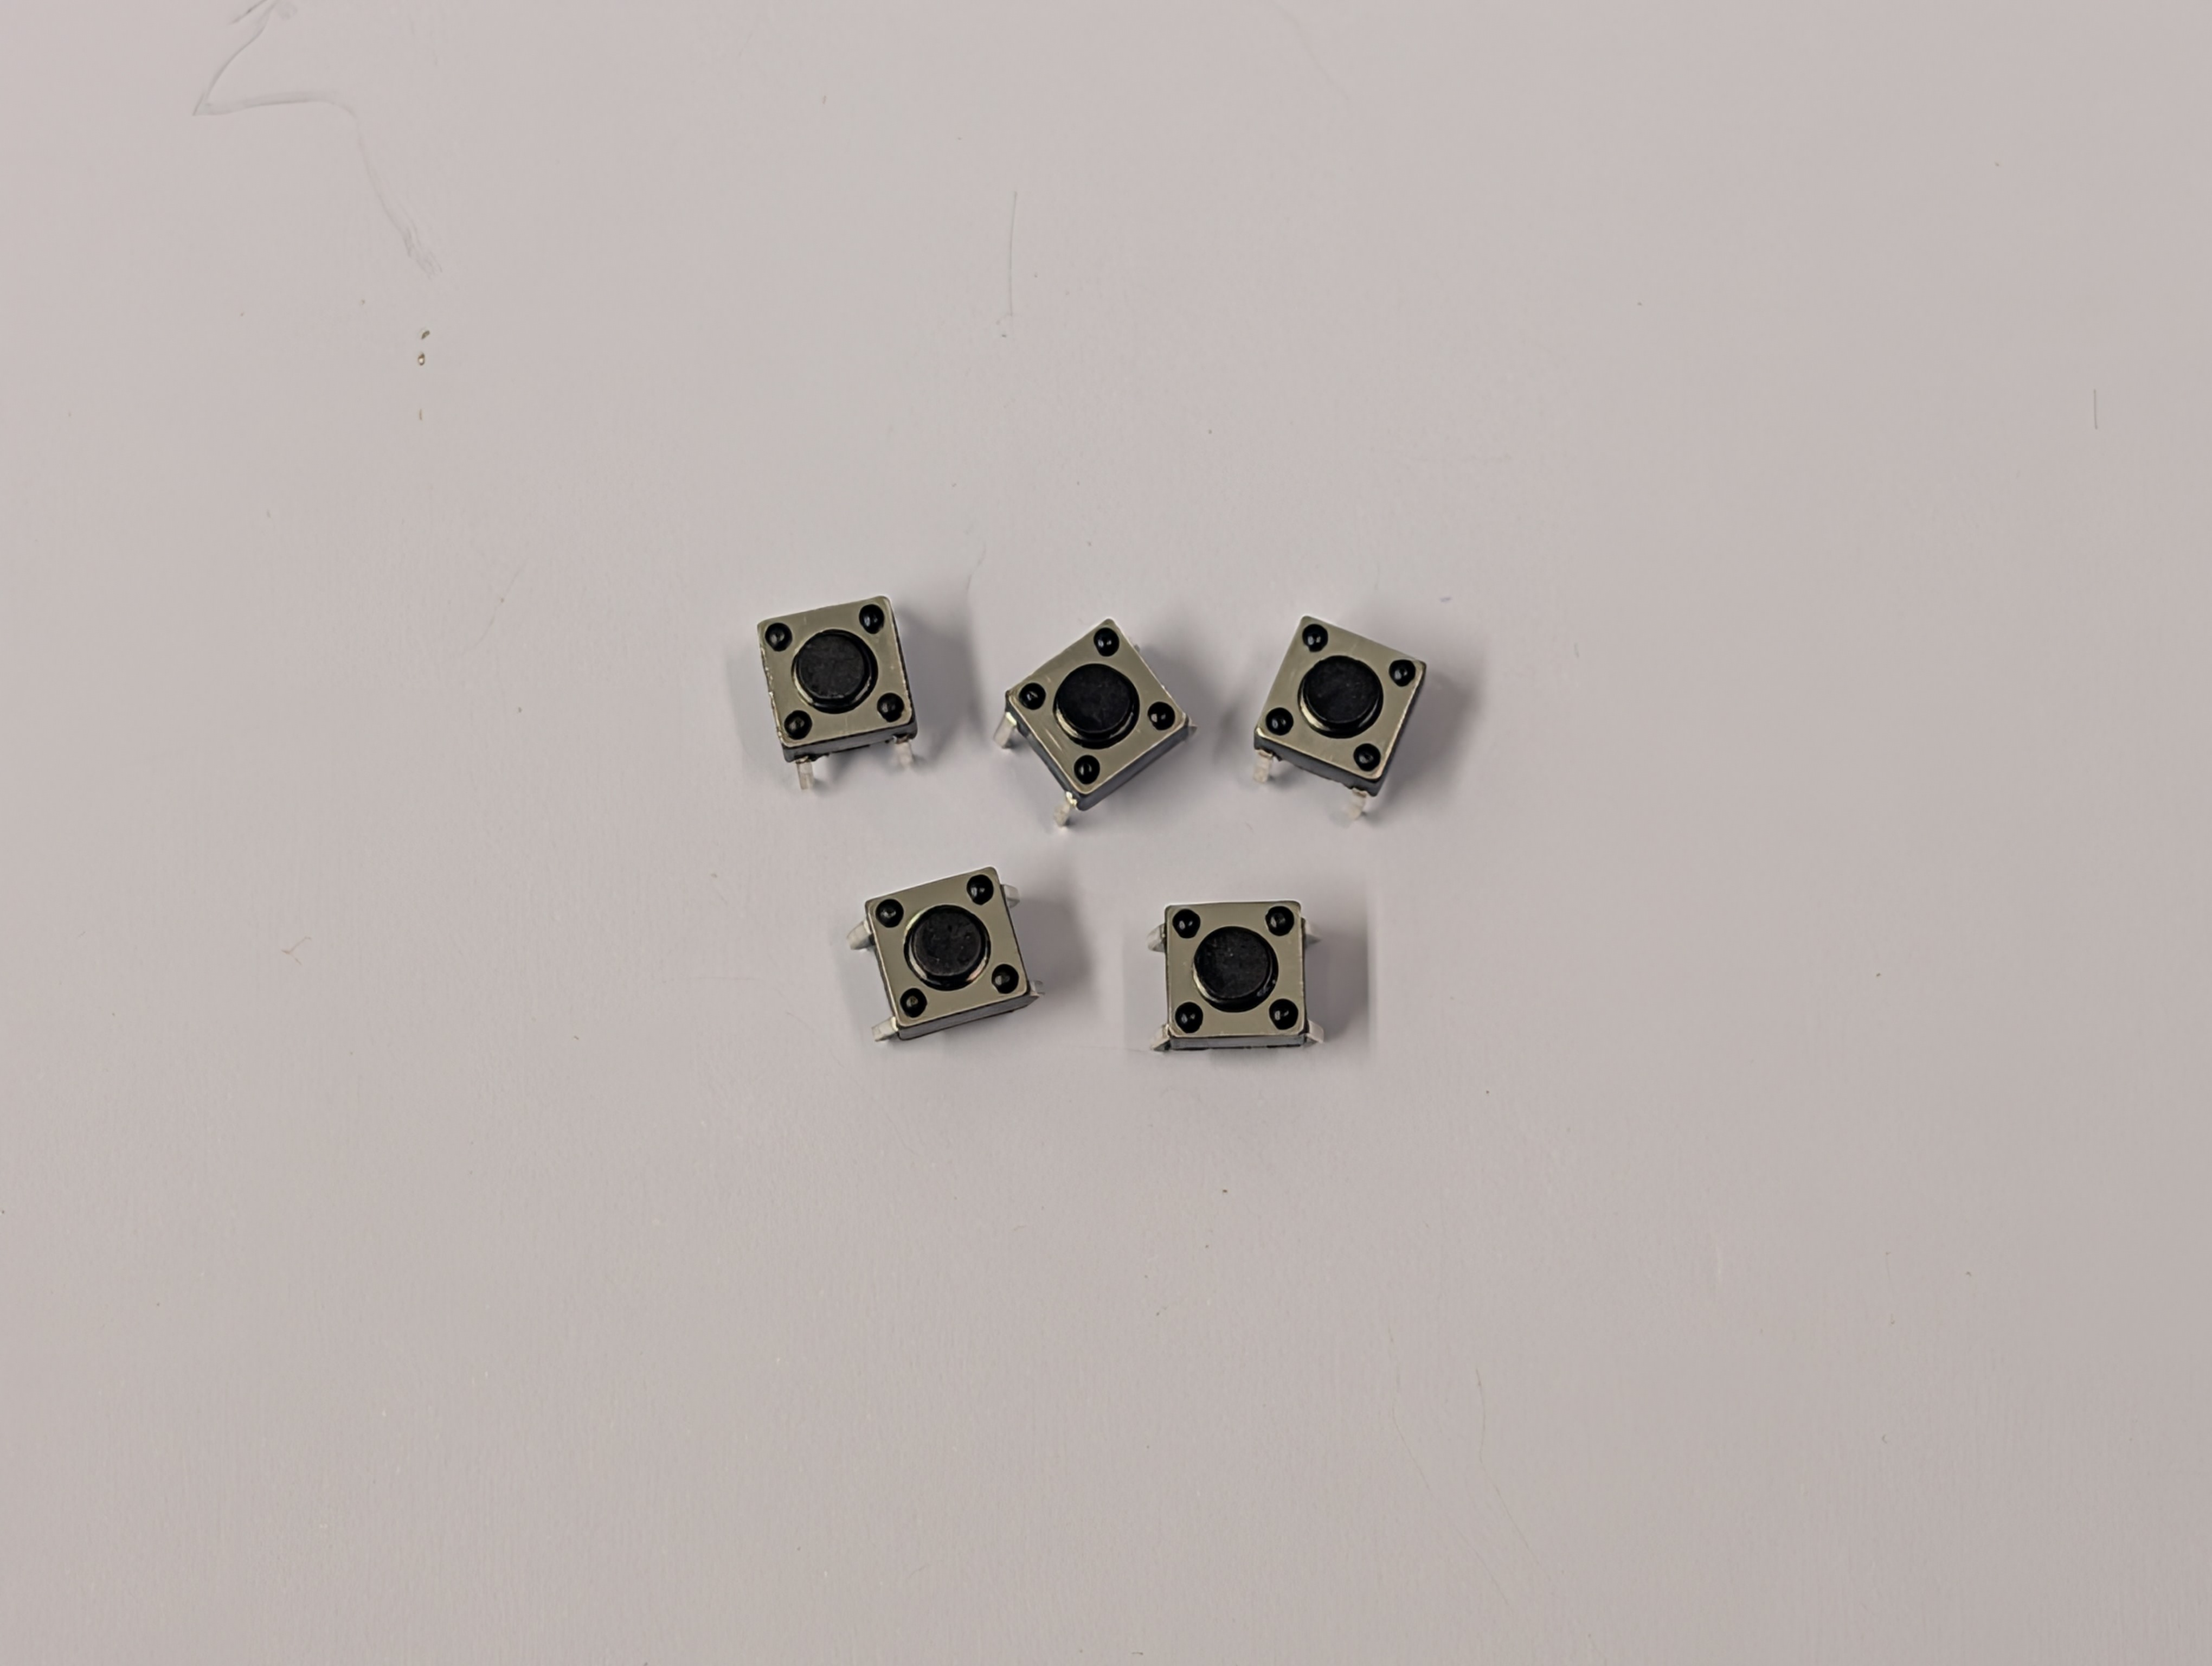
\includegraphics[width=0.75\textwidth]{pictures_of_construction/instruction_step_40.jpg}
\end{figure}

For the assembly of the Buzzerino PCB, we will go from the shortest to the highest component. This helps you successfully solder your board.

\begin{figure}[H]
    \centering
    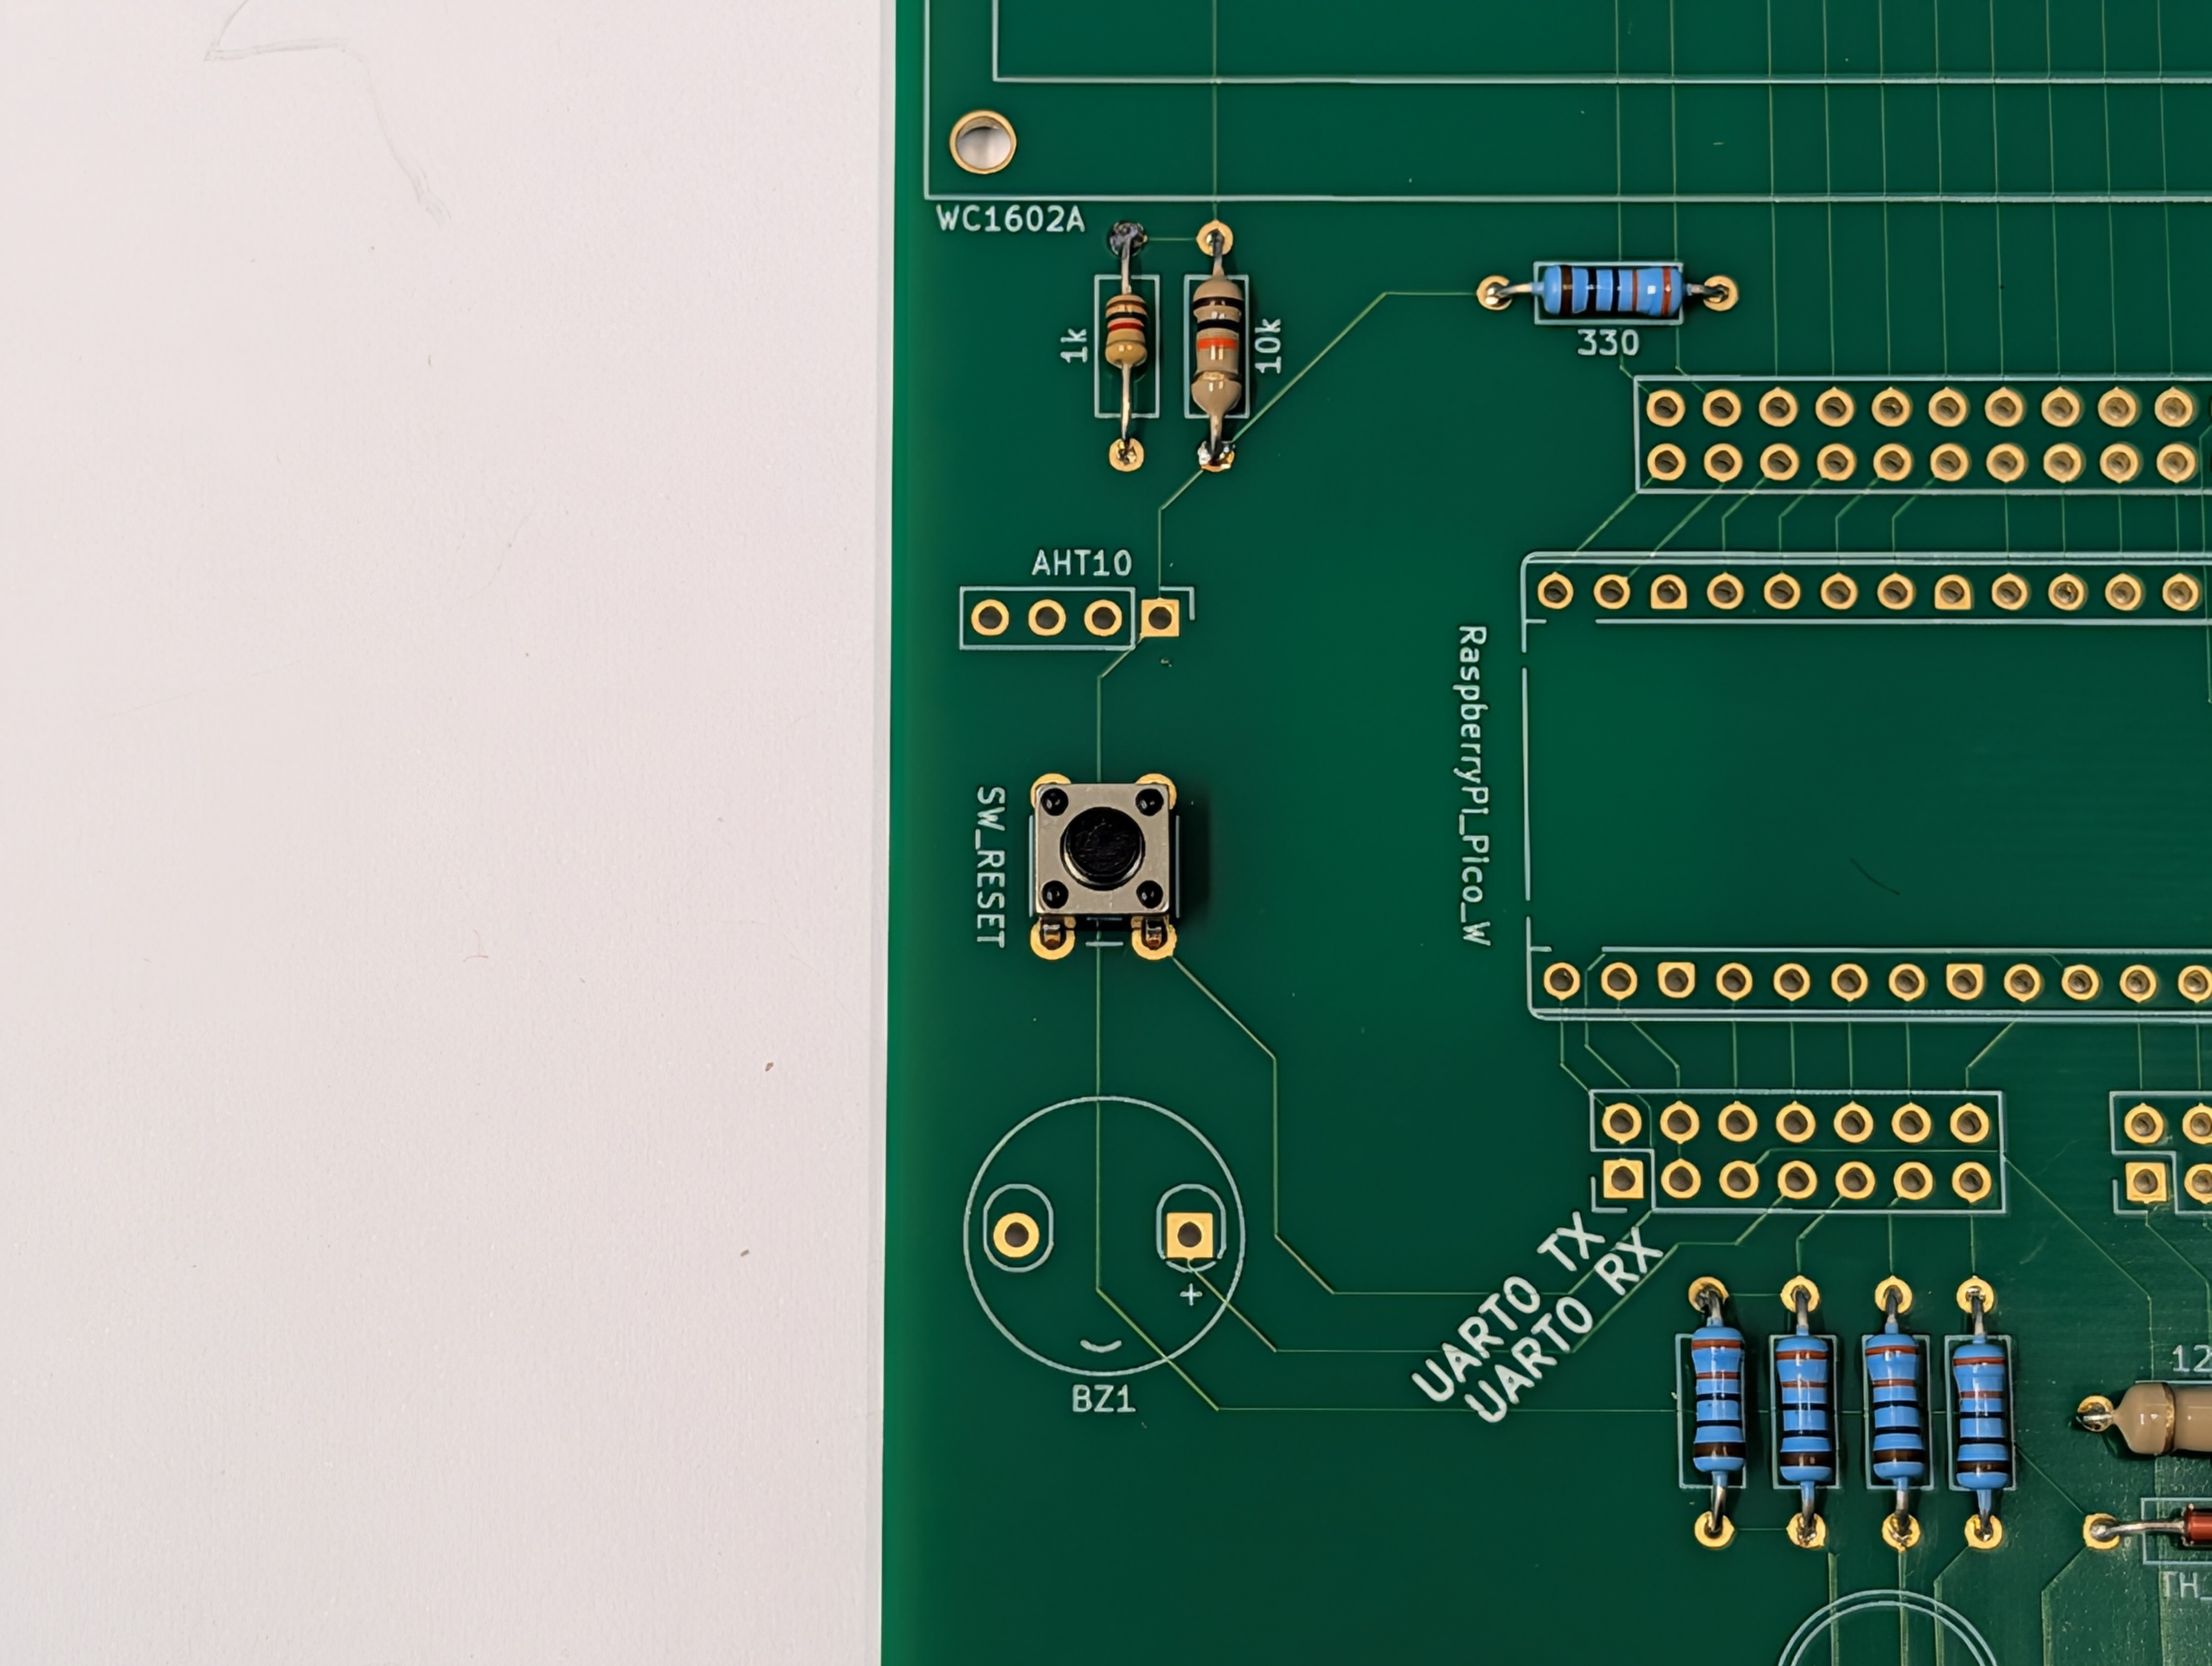
\includegraphics[width=0.75\textwidth]{pictures_of_construction/instruction_step_41.jpg}
\end{figure}

\begin{figure}[H]
    \centering
    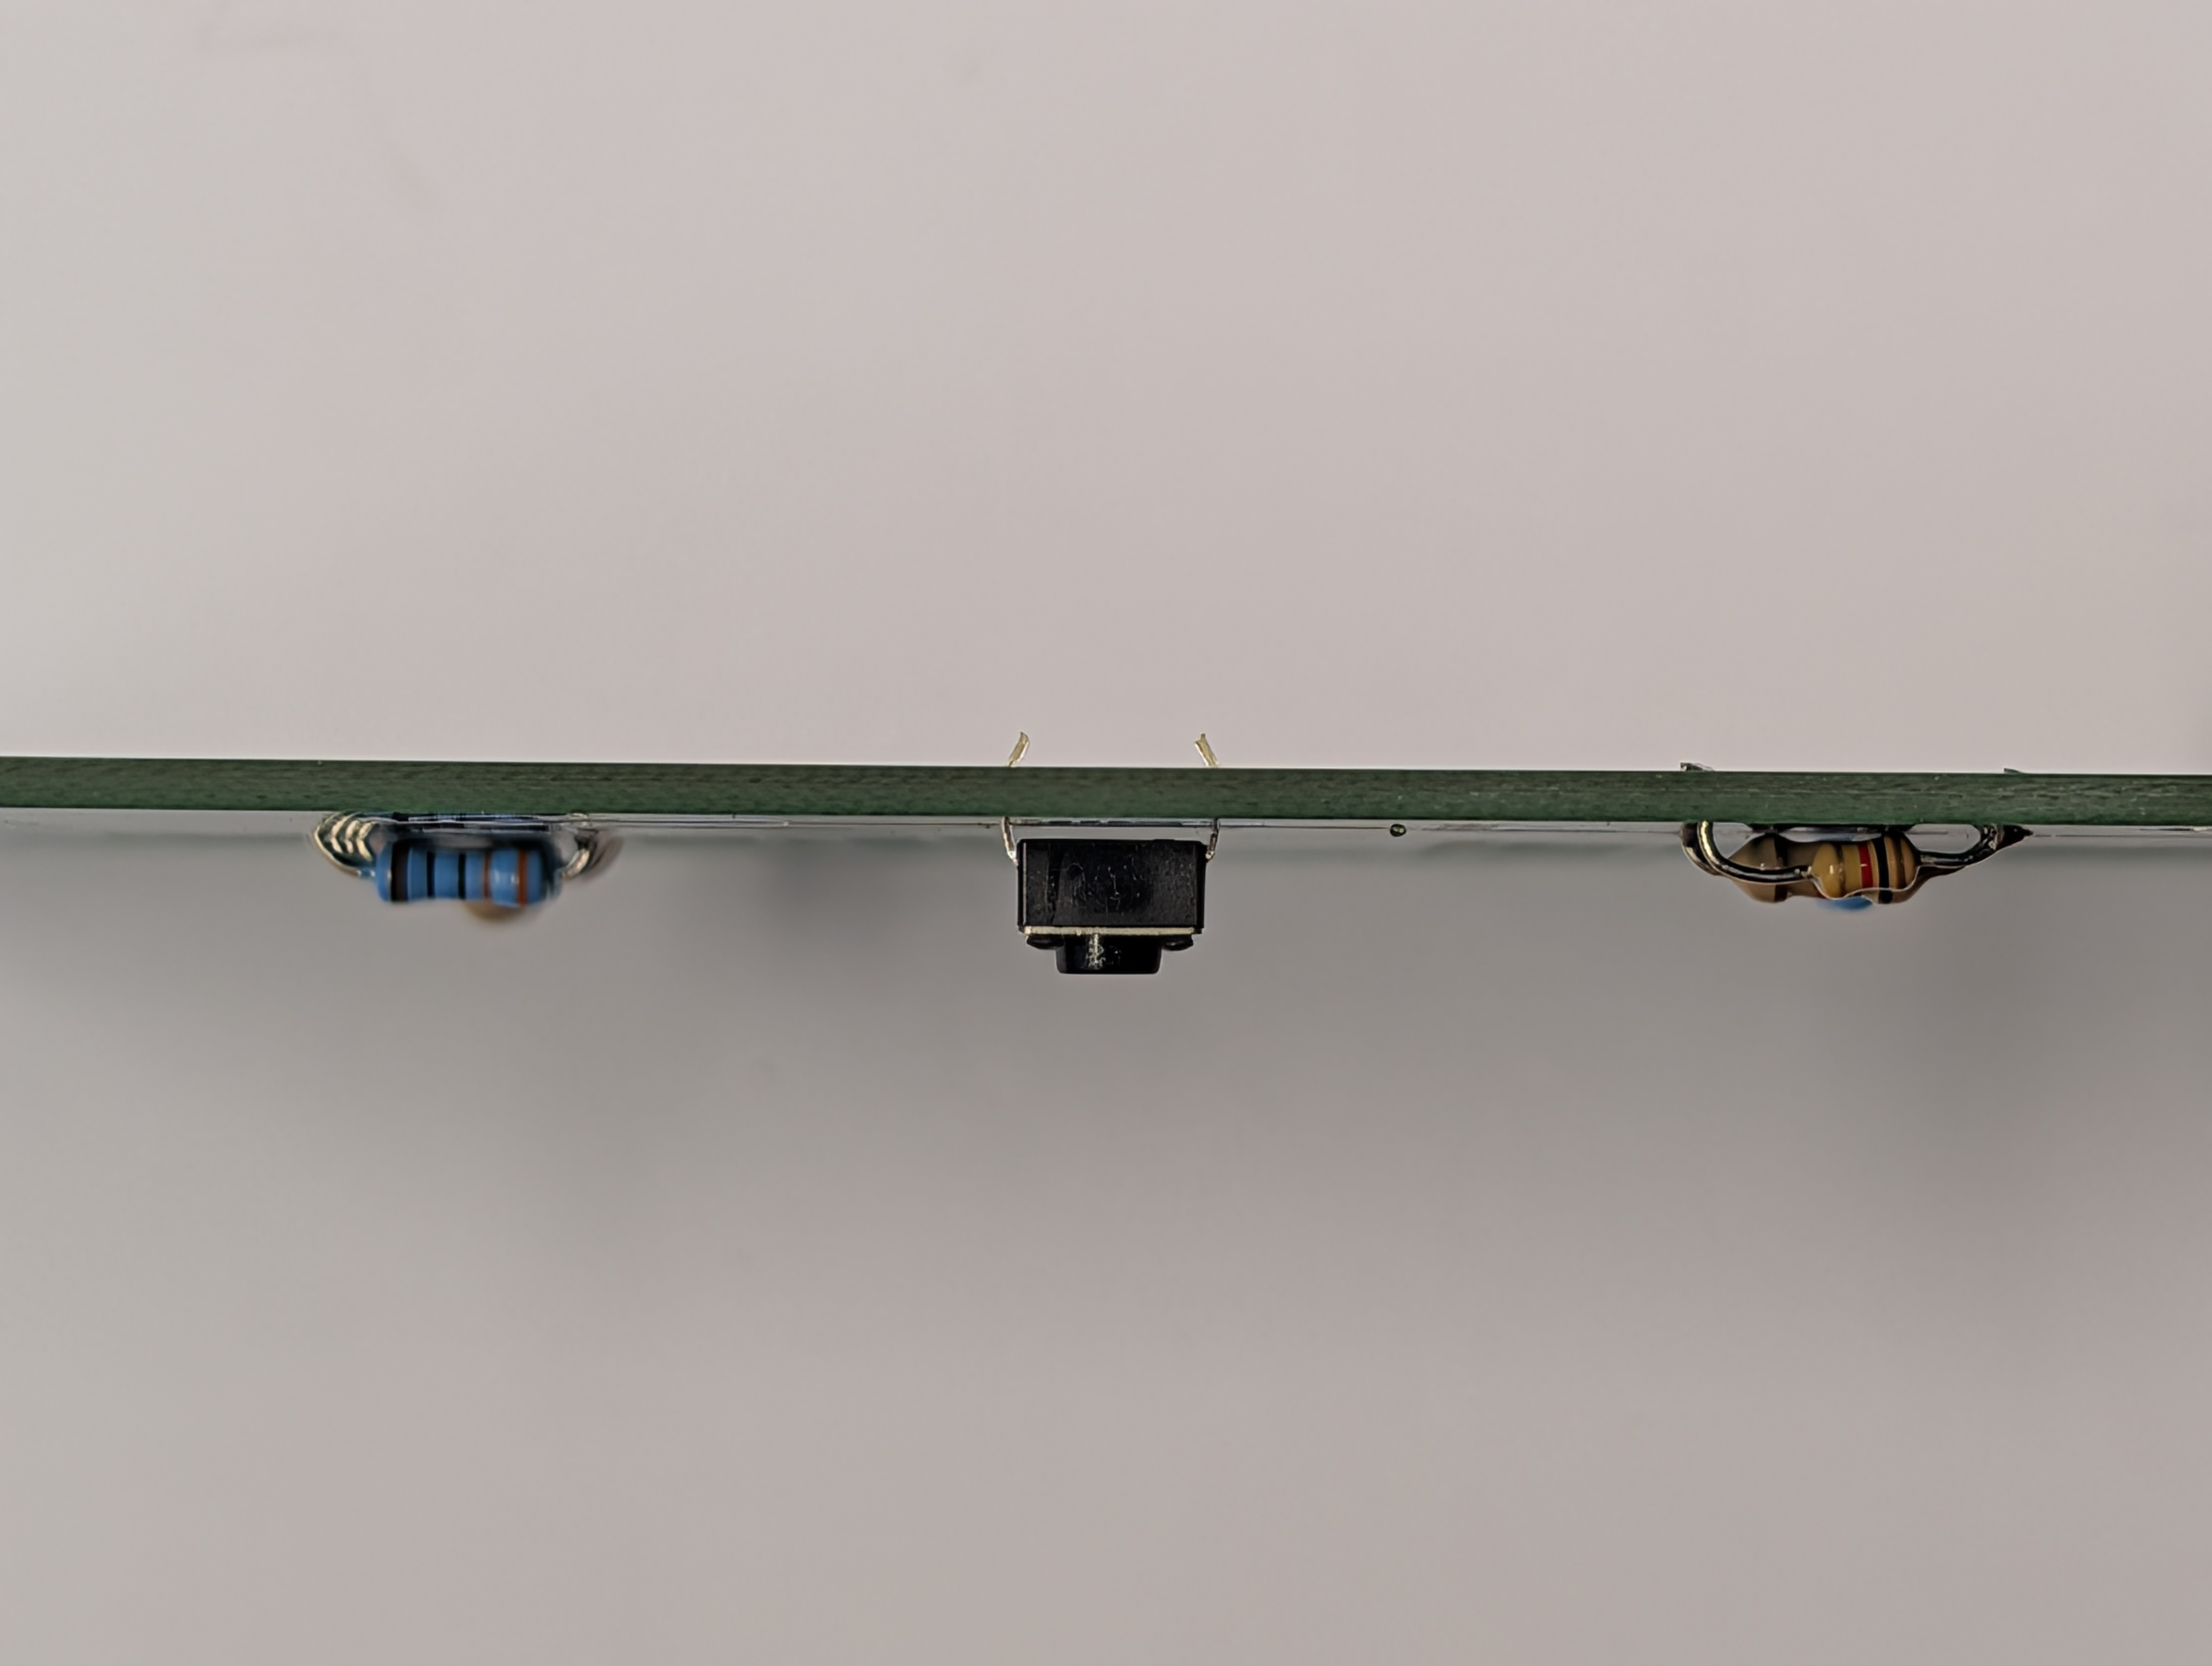
\includegraphics[width=0.75\textwidth]{pictures_of_construction/instruction_step_42.jpg}
\end{figure}

The shape of the button legs is designed to snap into the Buzzerino PCB. After placing the buttons, check if they sit flush to the Buzzerino PCB. Then solder and clip the leads.

\begin{figure}[H]
    \centering
    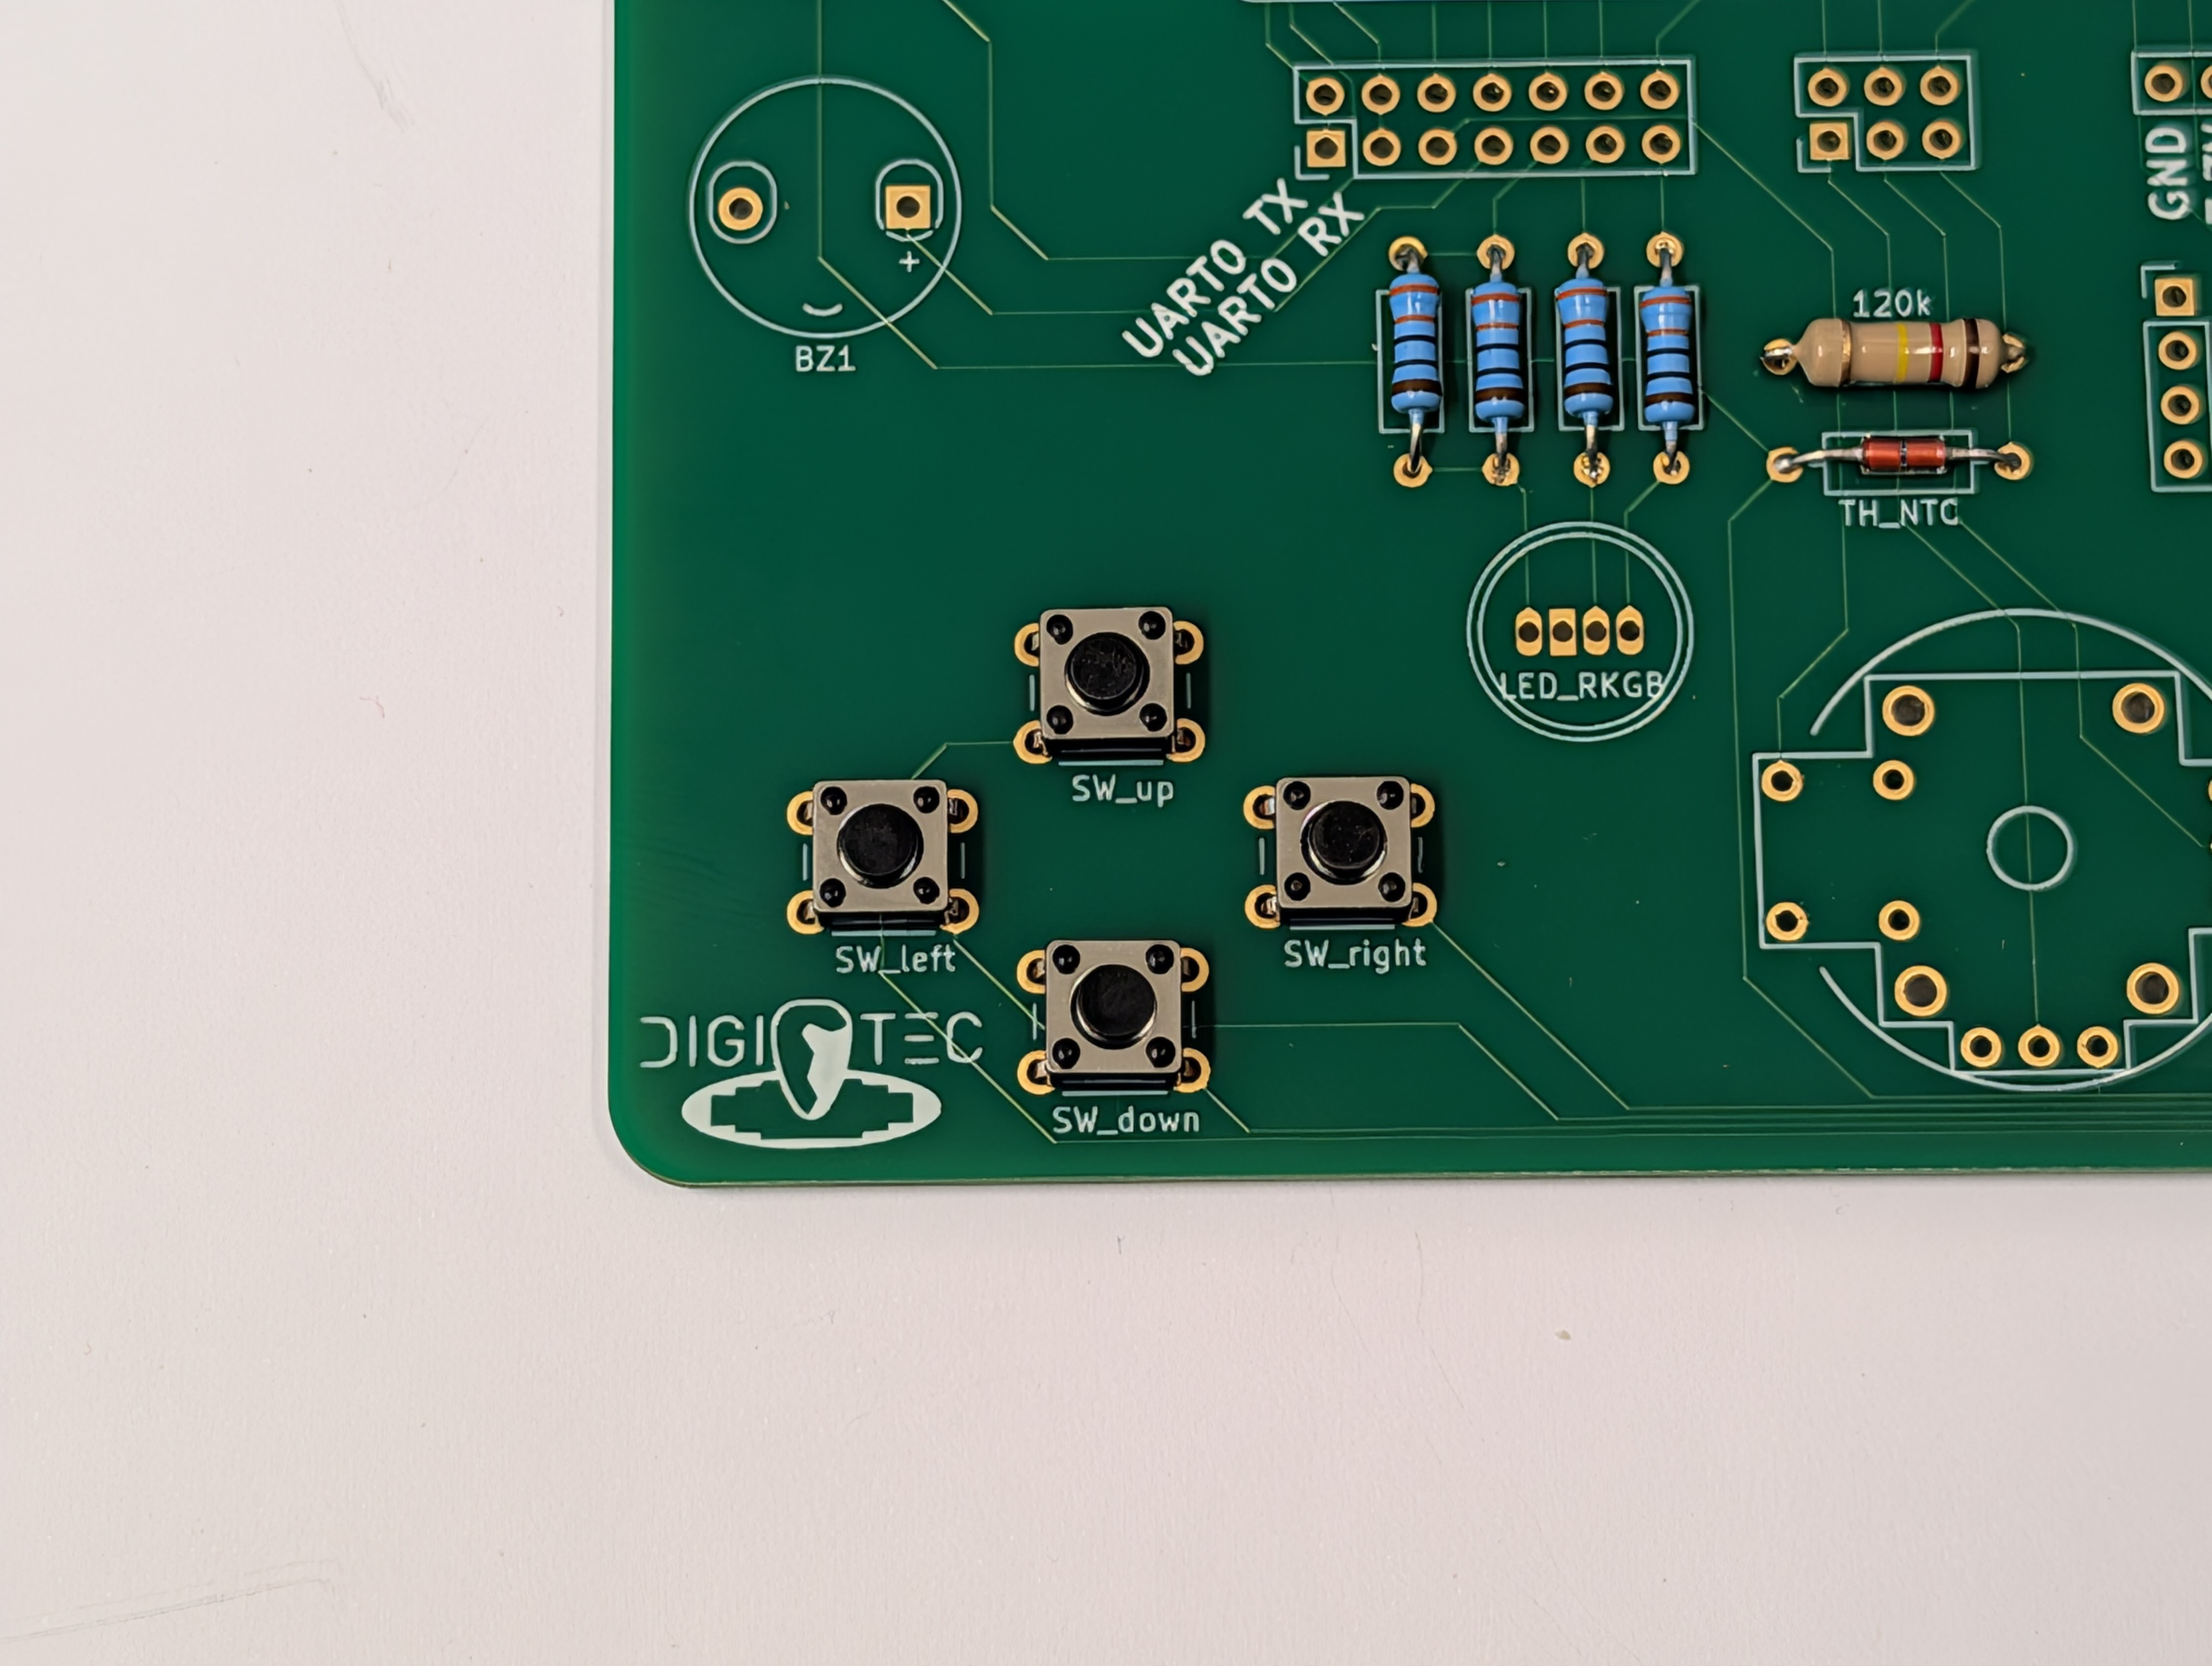
\includegraphics[width=0.75\textwidth]{pictures_of_construction/instruction_step_43.jpg}
\end{figure}

With the D-pad buttons it is the same procedure as with the reset button.

\subsection*{Soldering the pin header}

\textbf{Repeated Error: The short side shall go through the board!}

\begin{figure}[H]
    \centering
    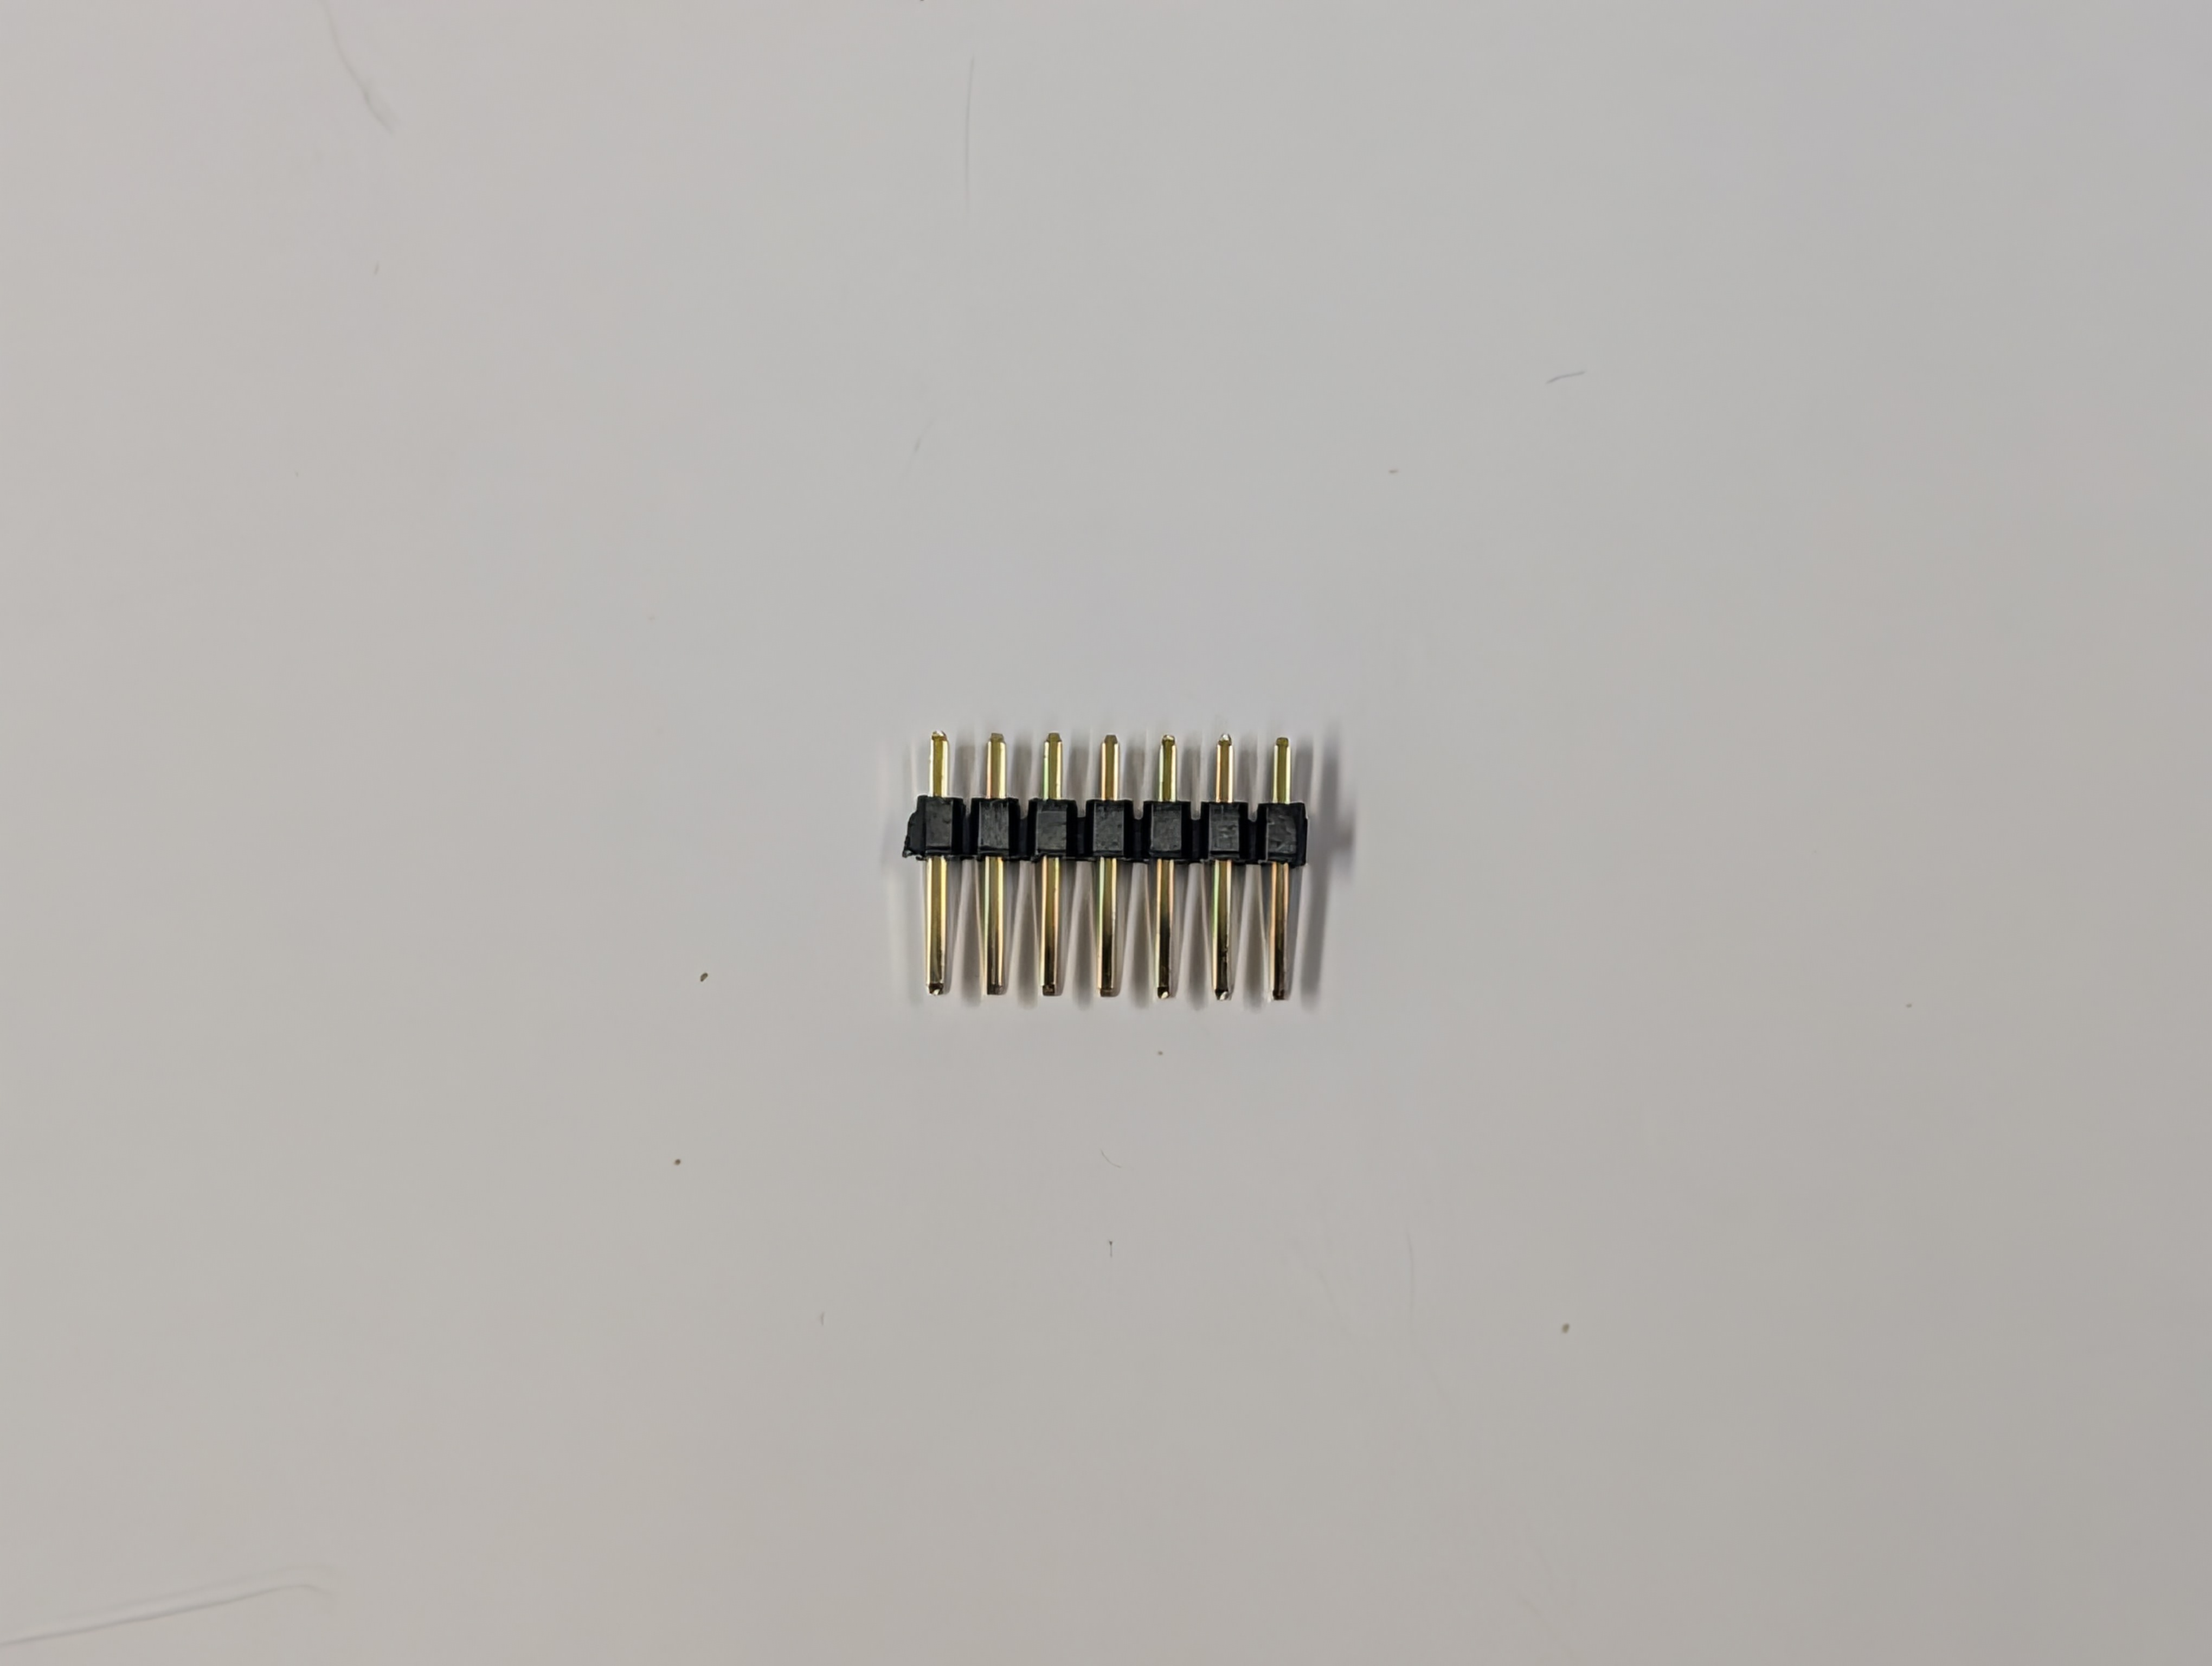
\includegraphics[width=0.75\textwidth]{pictures_of_construction/instruction_step_44.jpg}
\end{figure}

\begin{figure}[H]
    \centering
    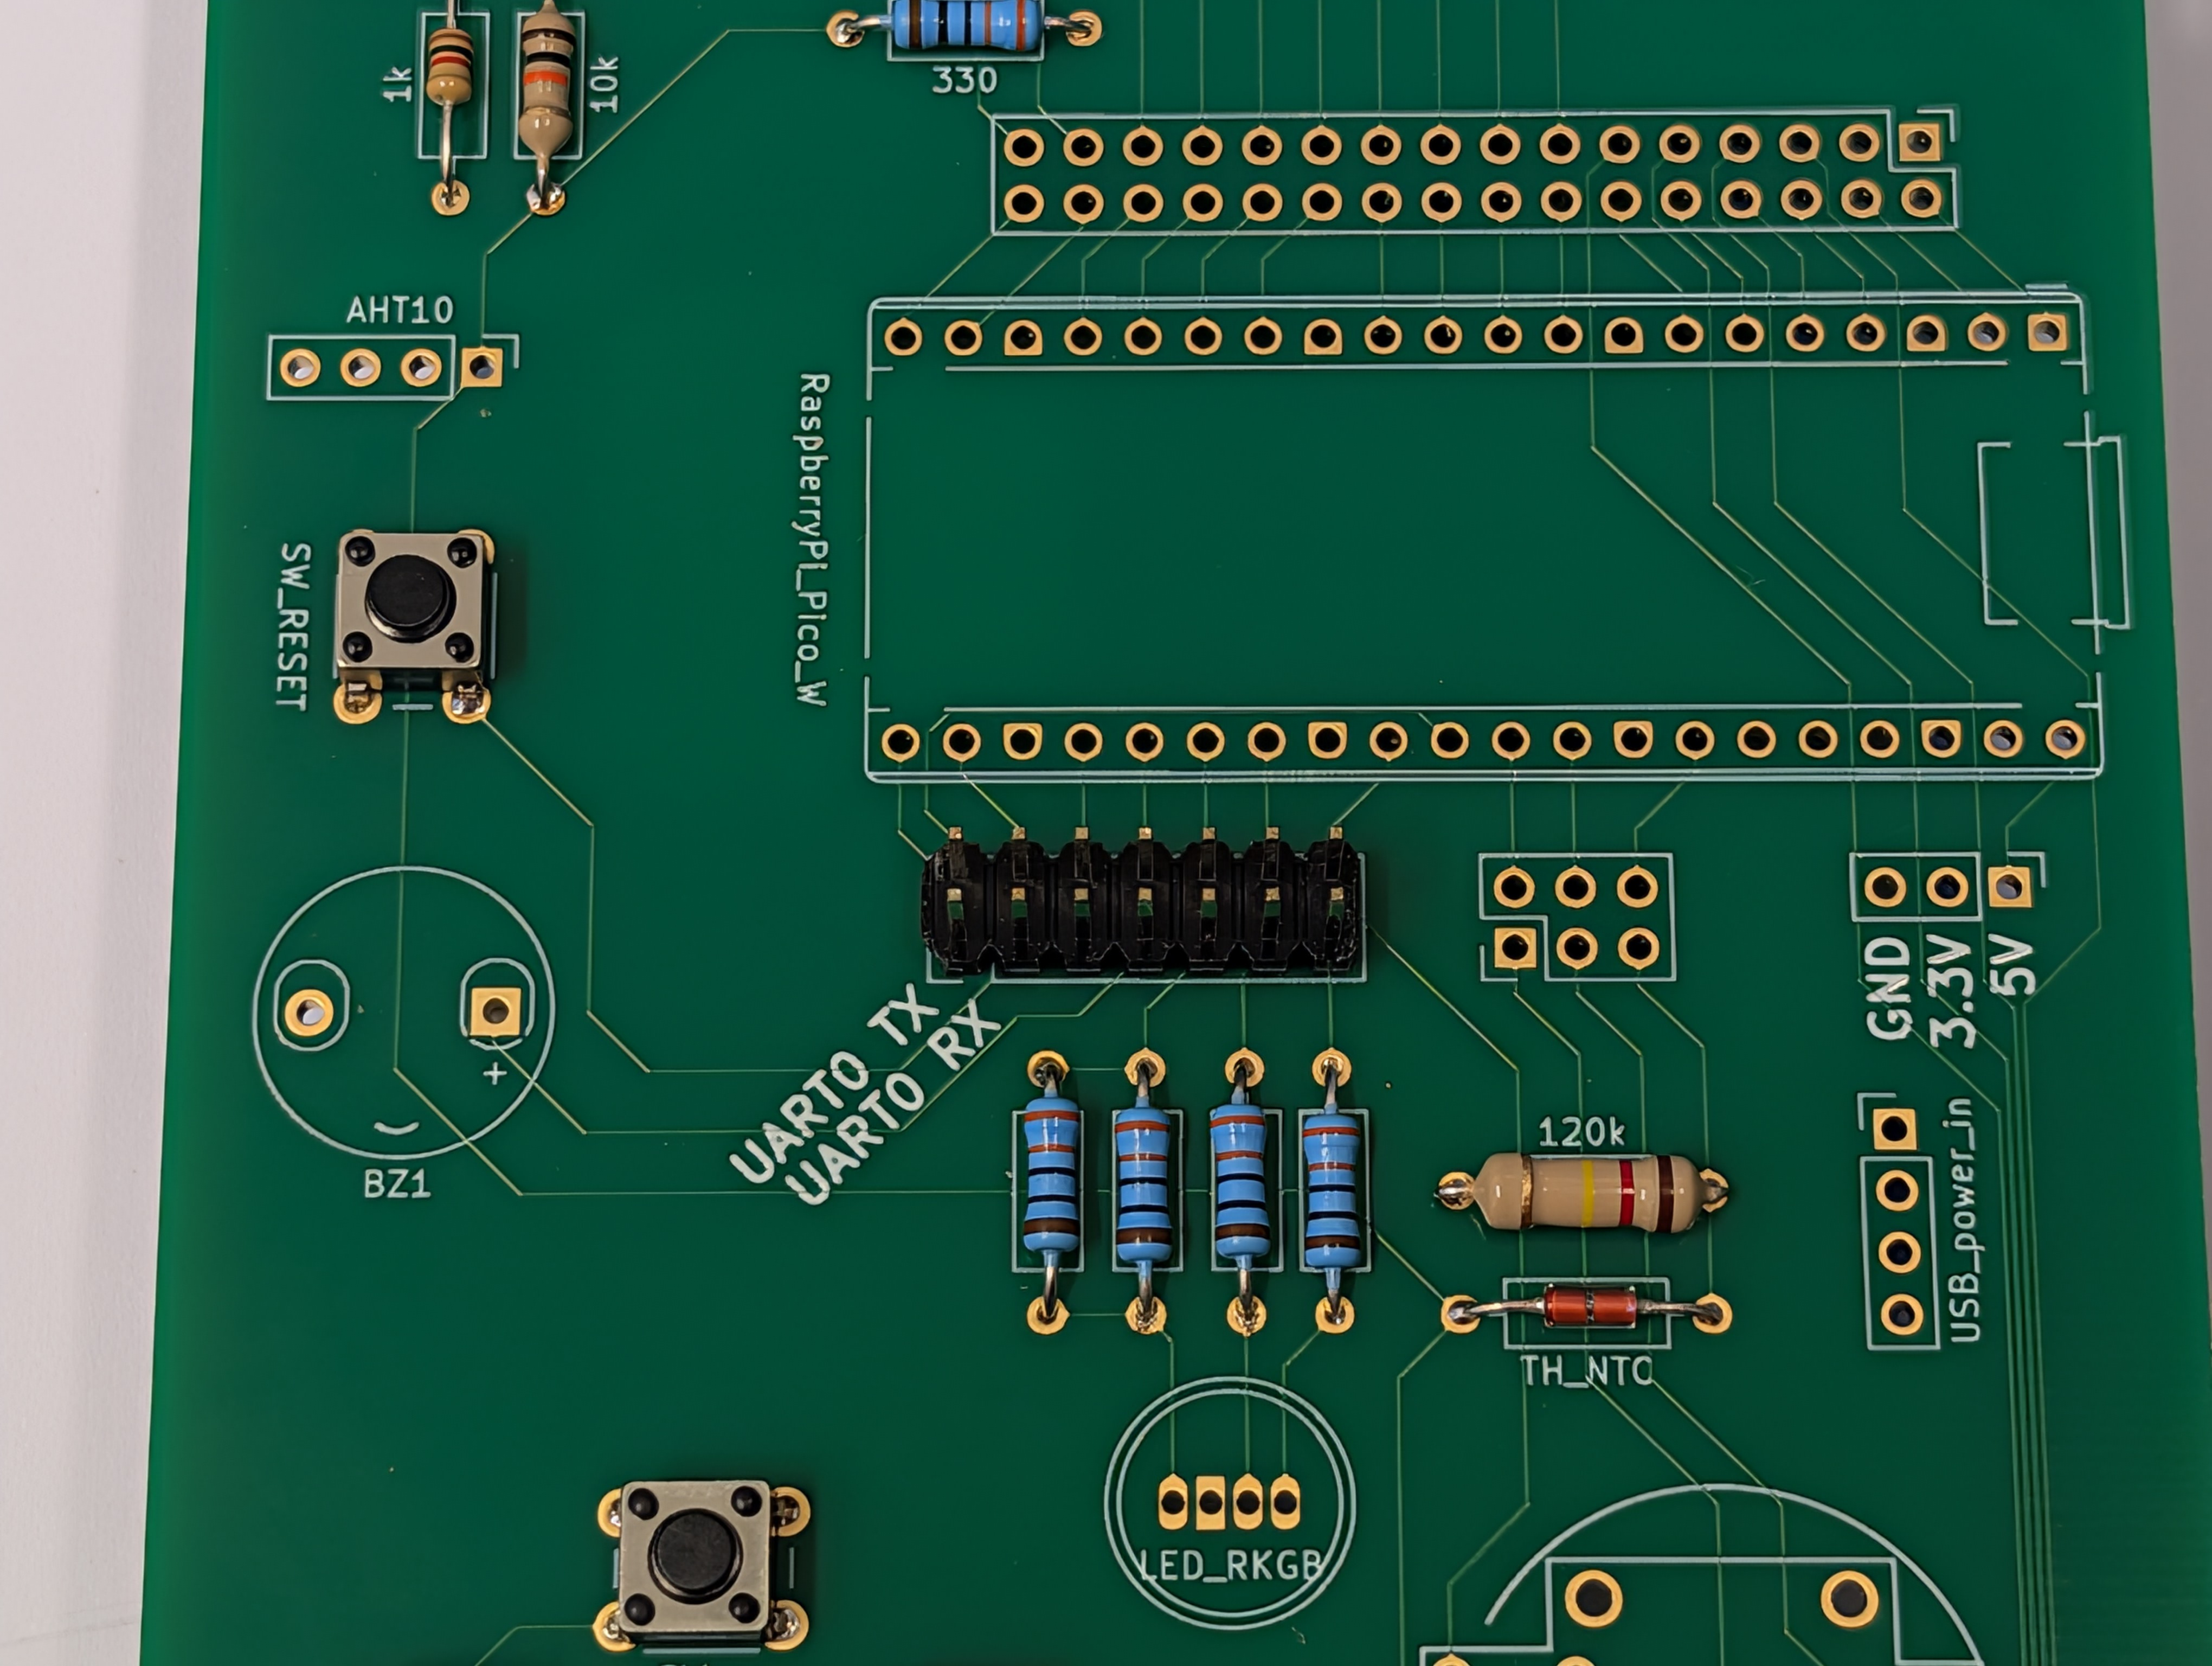
\includegraphics[width=0.75\textwidth]{pictures_of_construction/instruction_step_45.jpg}
\end{figure}

We start by soldering the 2x7 pin header to the Buzzerino PCB. \textbf{The short side shall go through the board.}

\begin{figure}[H]
    \centering
    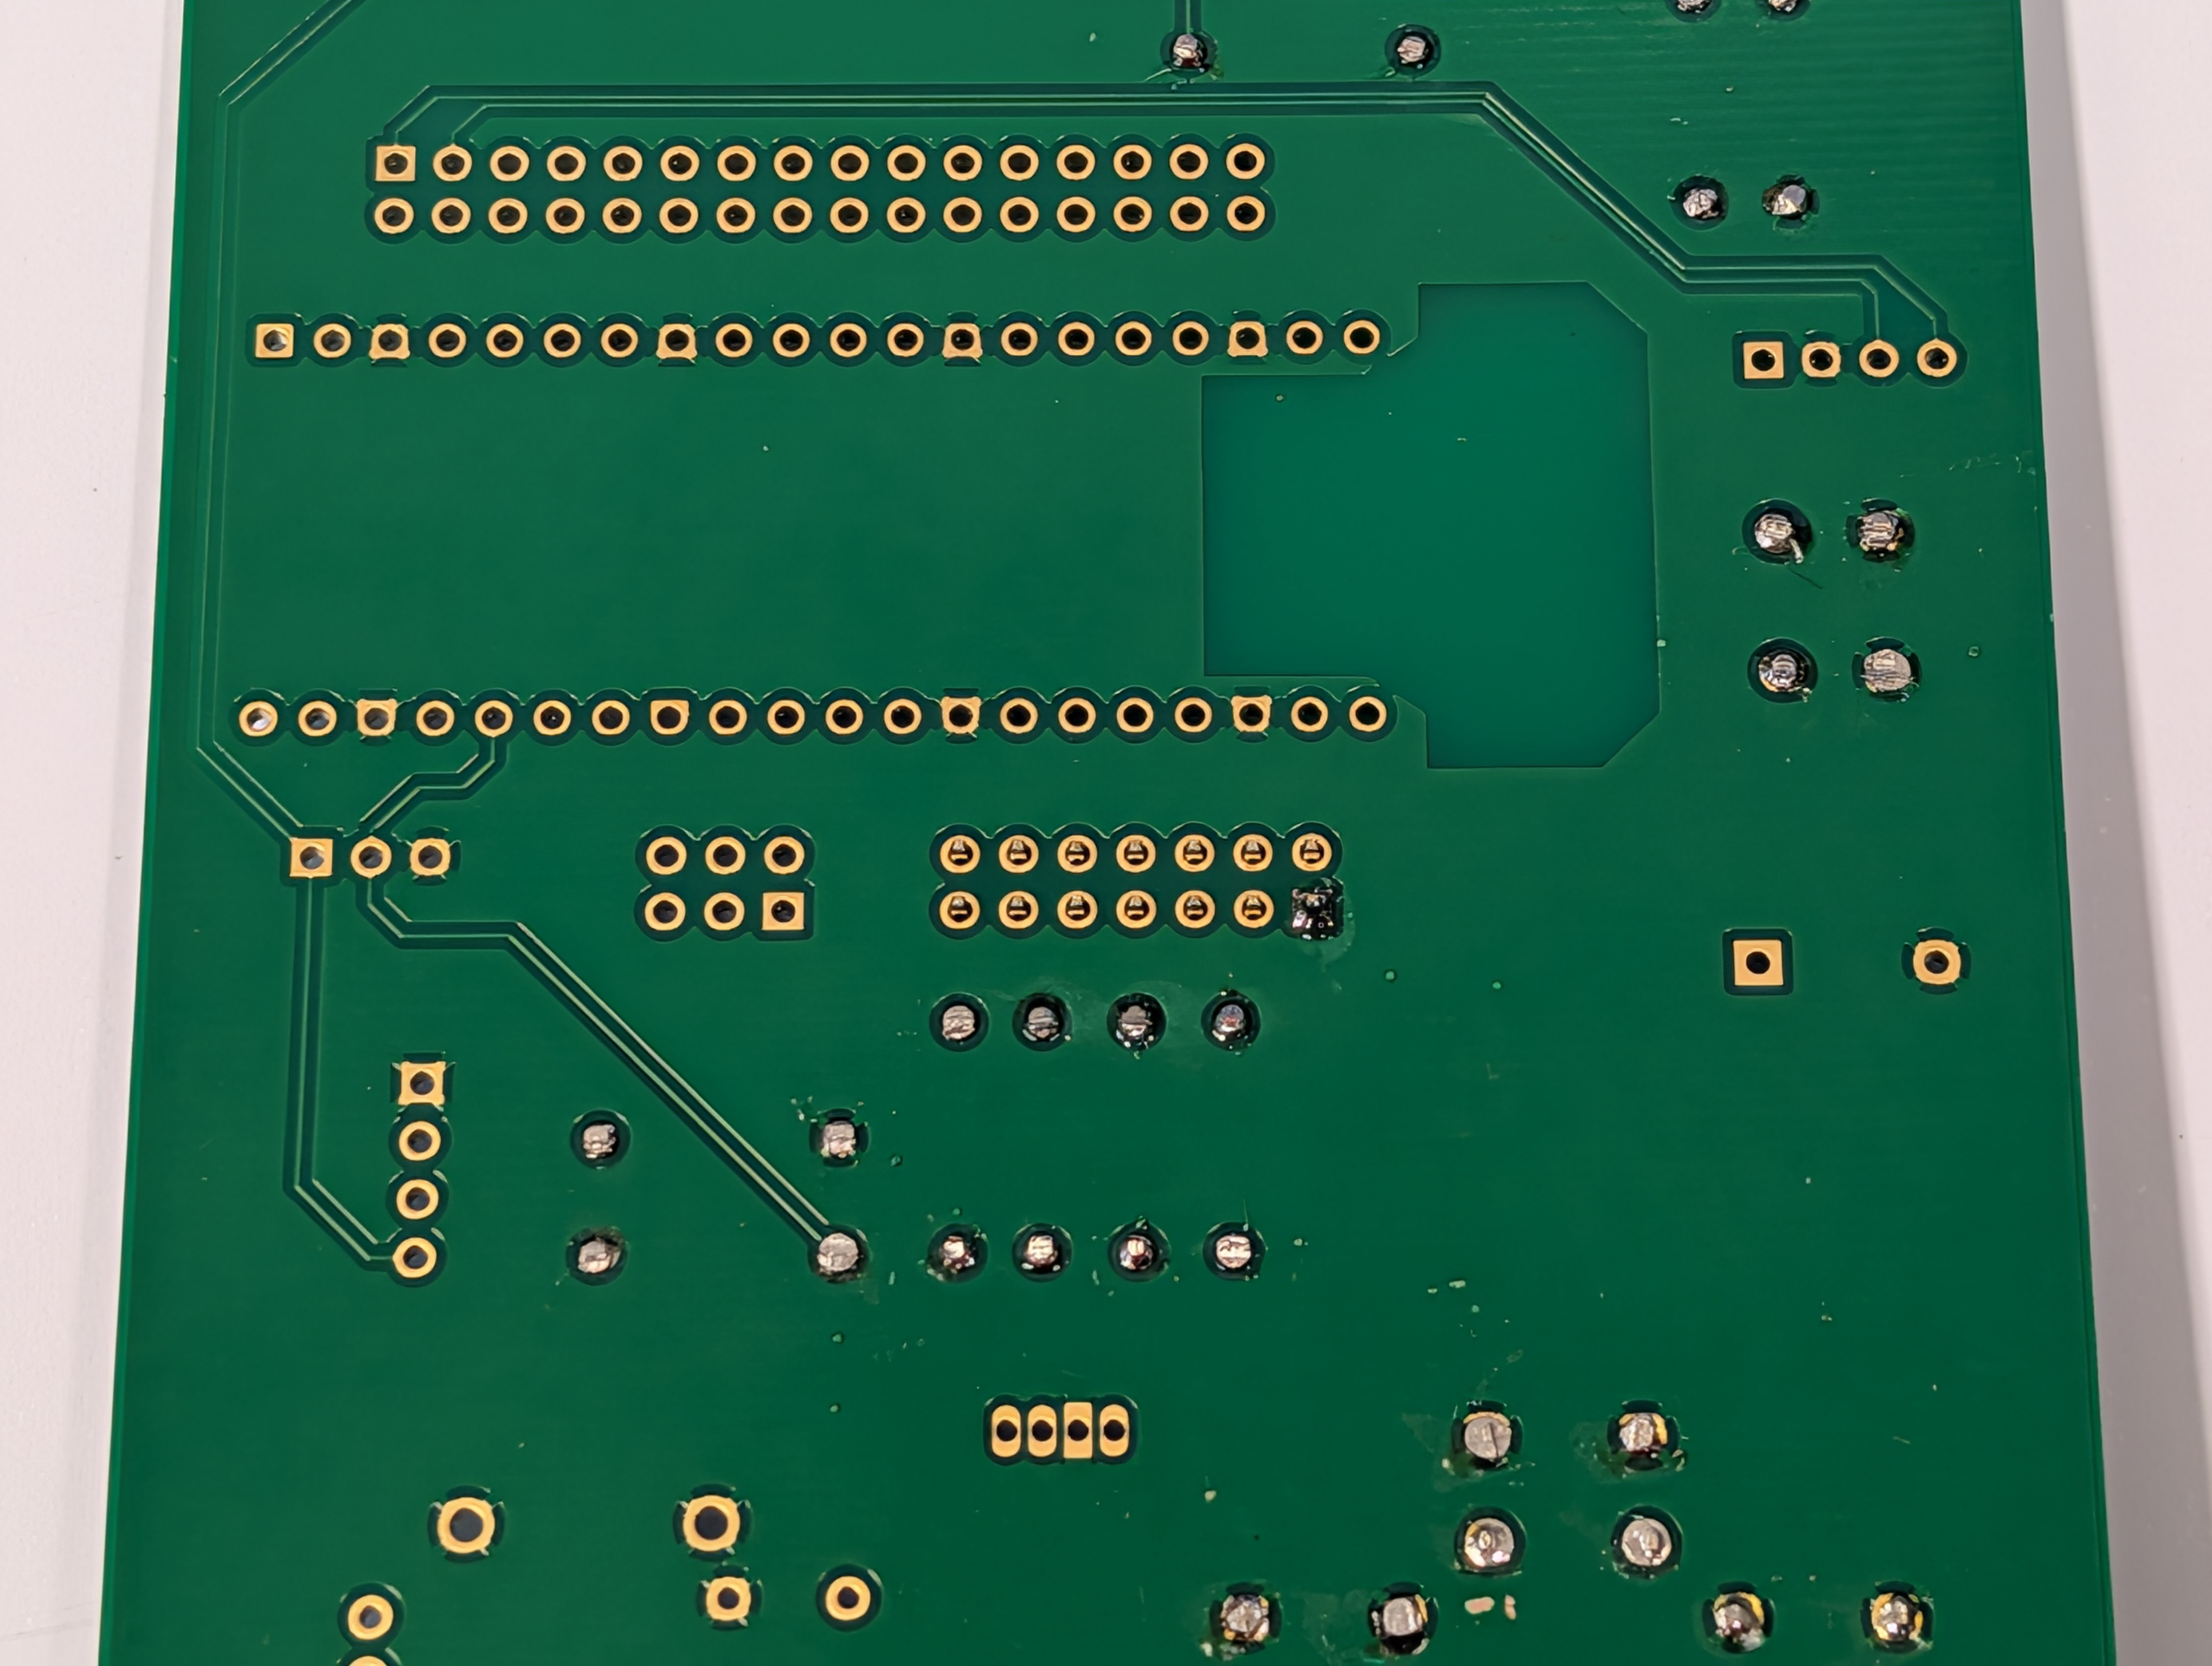
\includegraphics[width=0.75\textwidth]{pictures_of_construction/instruction_step_46.jpg}
\end{figure}

As with all the previous solder joints, it is best practice to first solder one pin and then check for alignment. The wider pin header will often move a bit out of the Buzzerino PCB and may need to be reseated. Only after the pin headers are placed completely in position should you solder the remaining pins.

\begin{figure}[H]
    \centering
    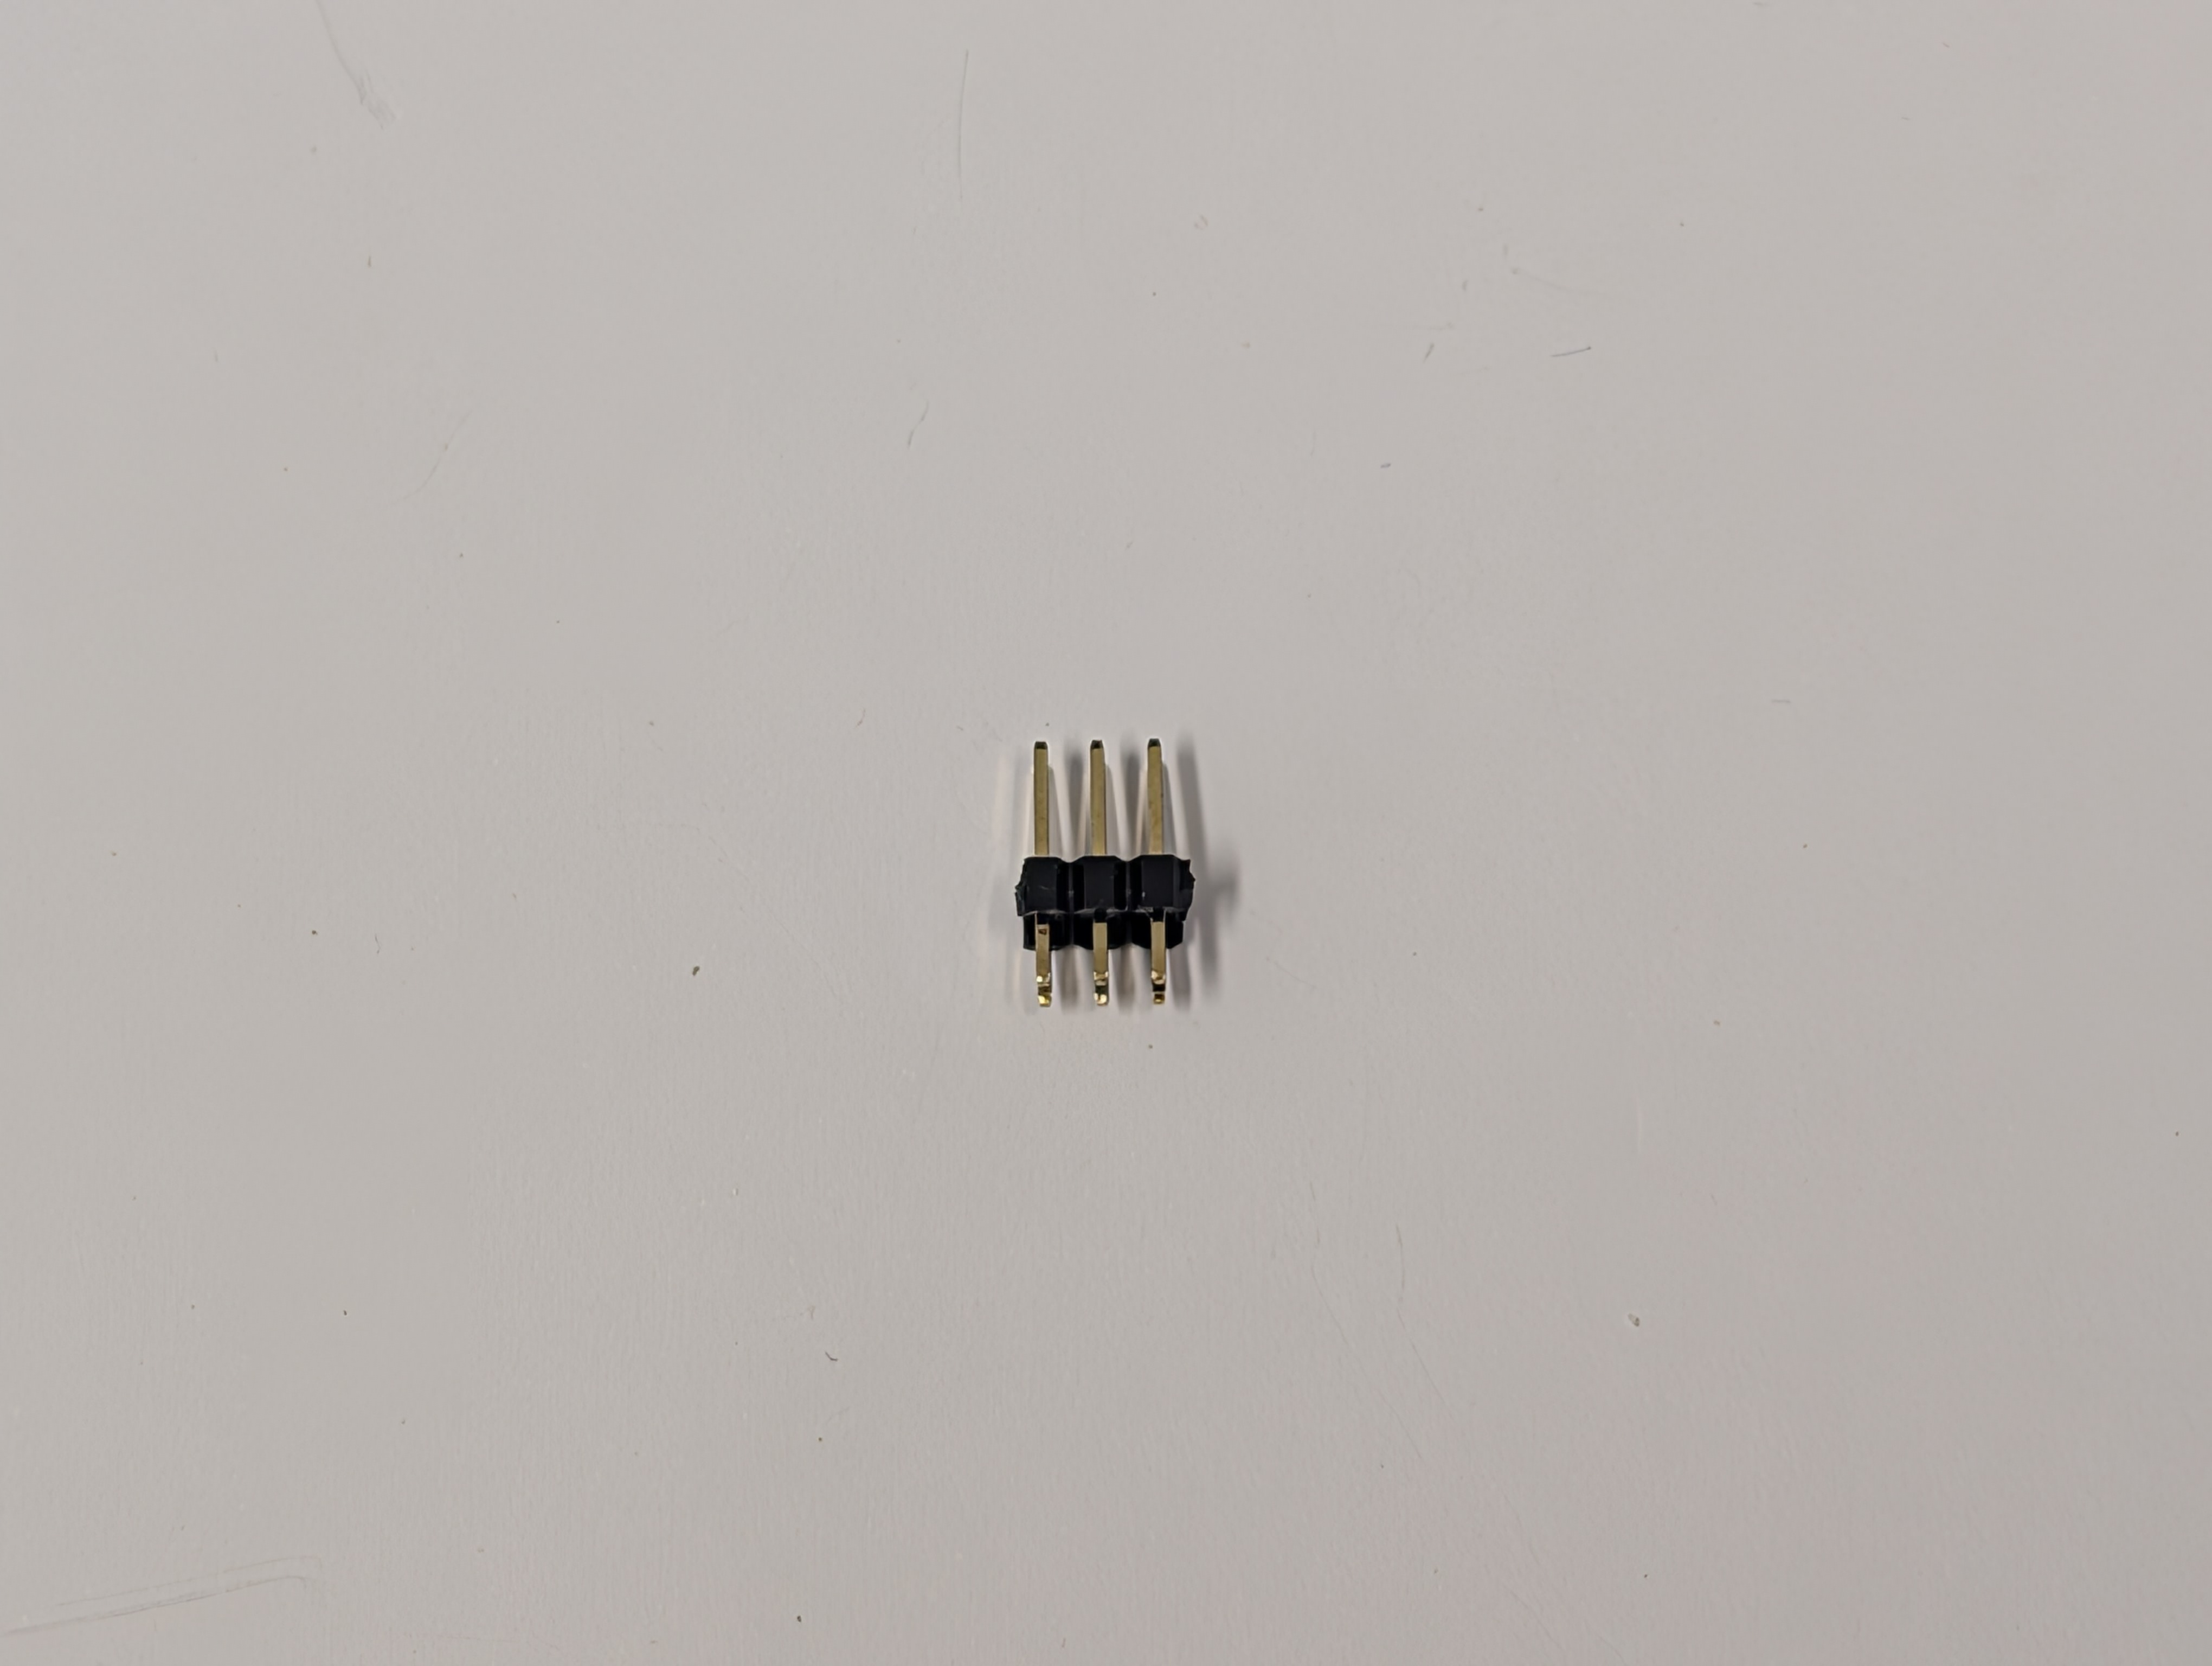
\includegraphics[width=0.75\textwidth]{pictures_of_construction/instruction_step_47.jpg}
\end{figure}

\begin{figure}[H]
    \centering
    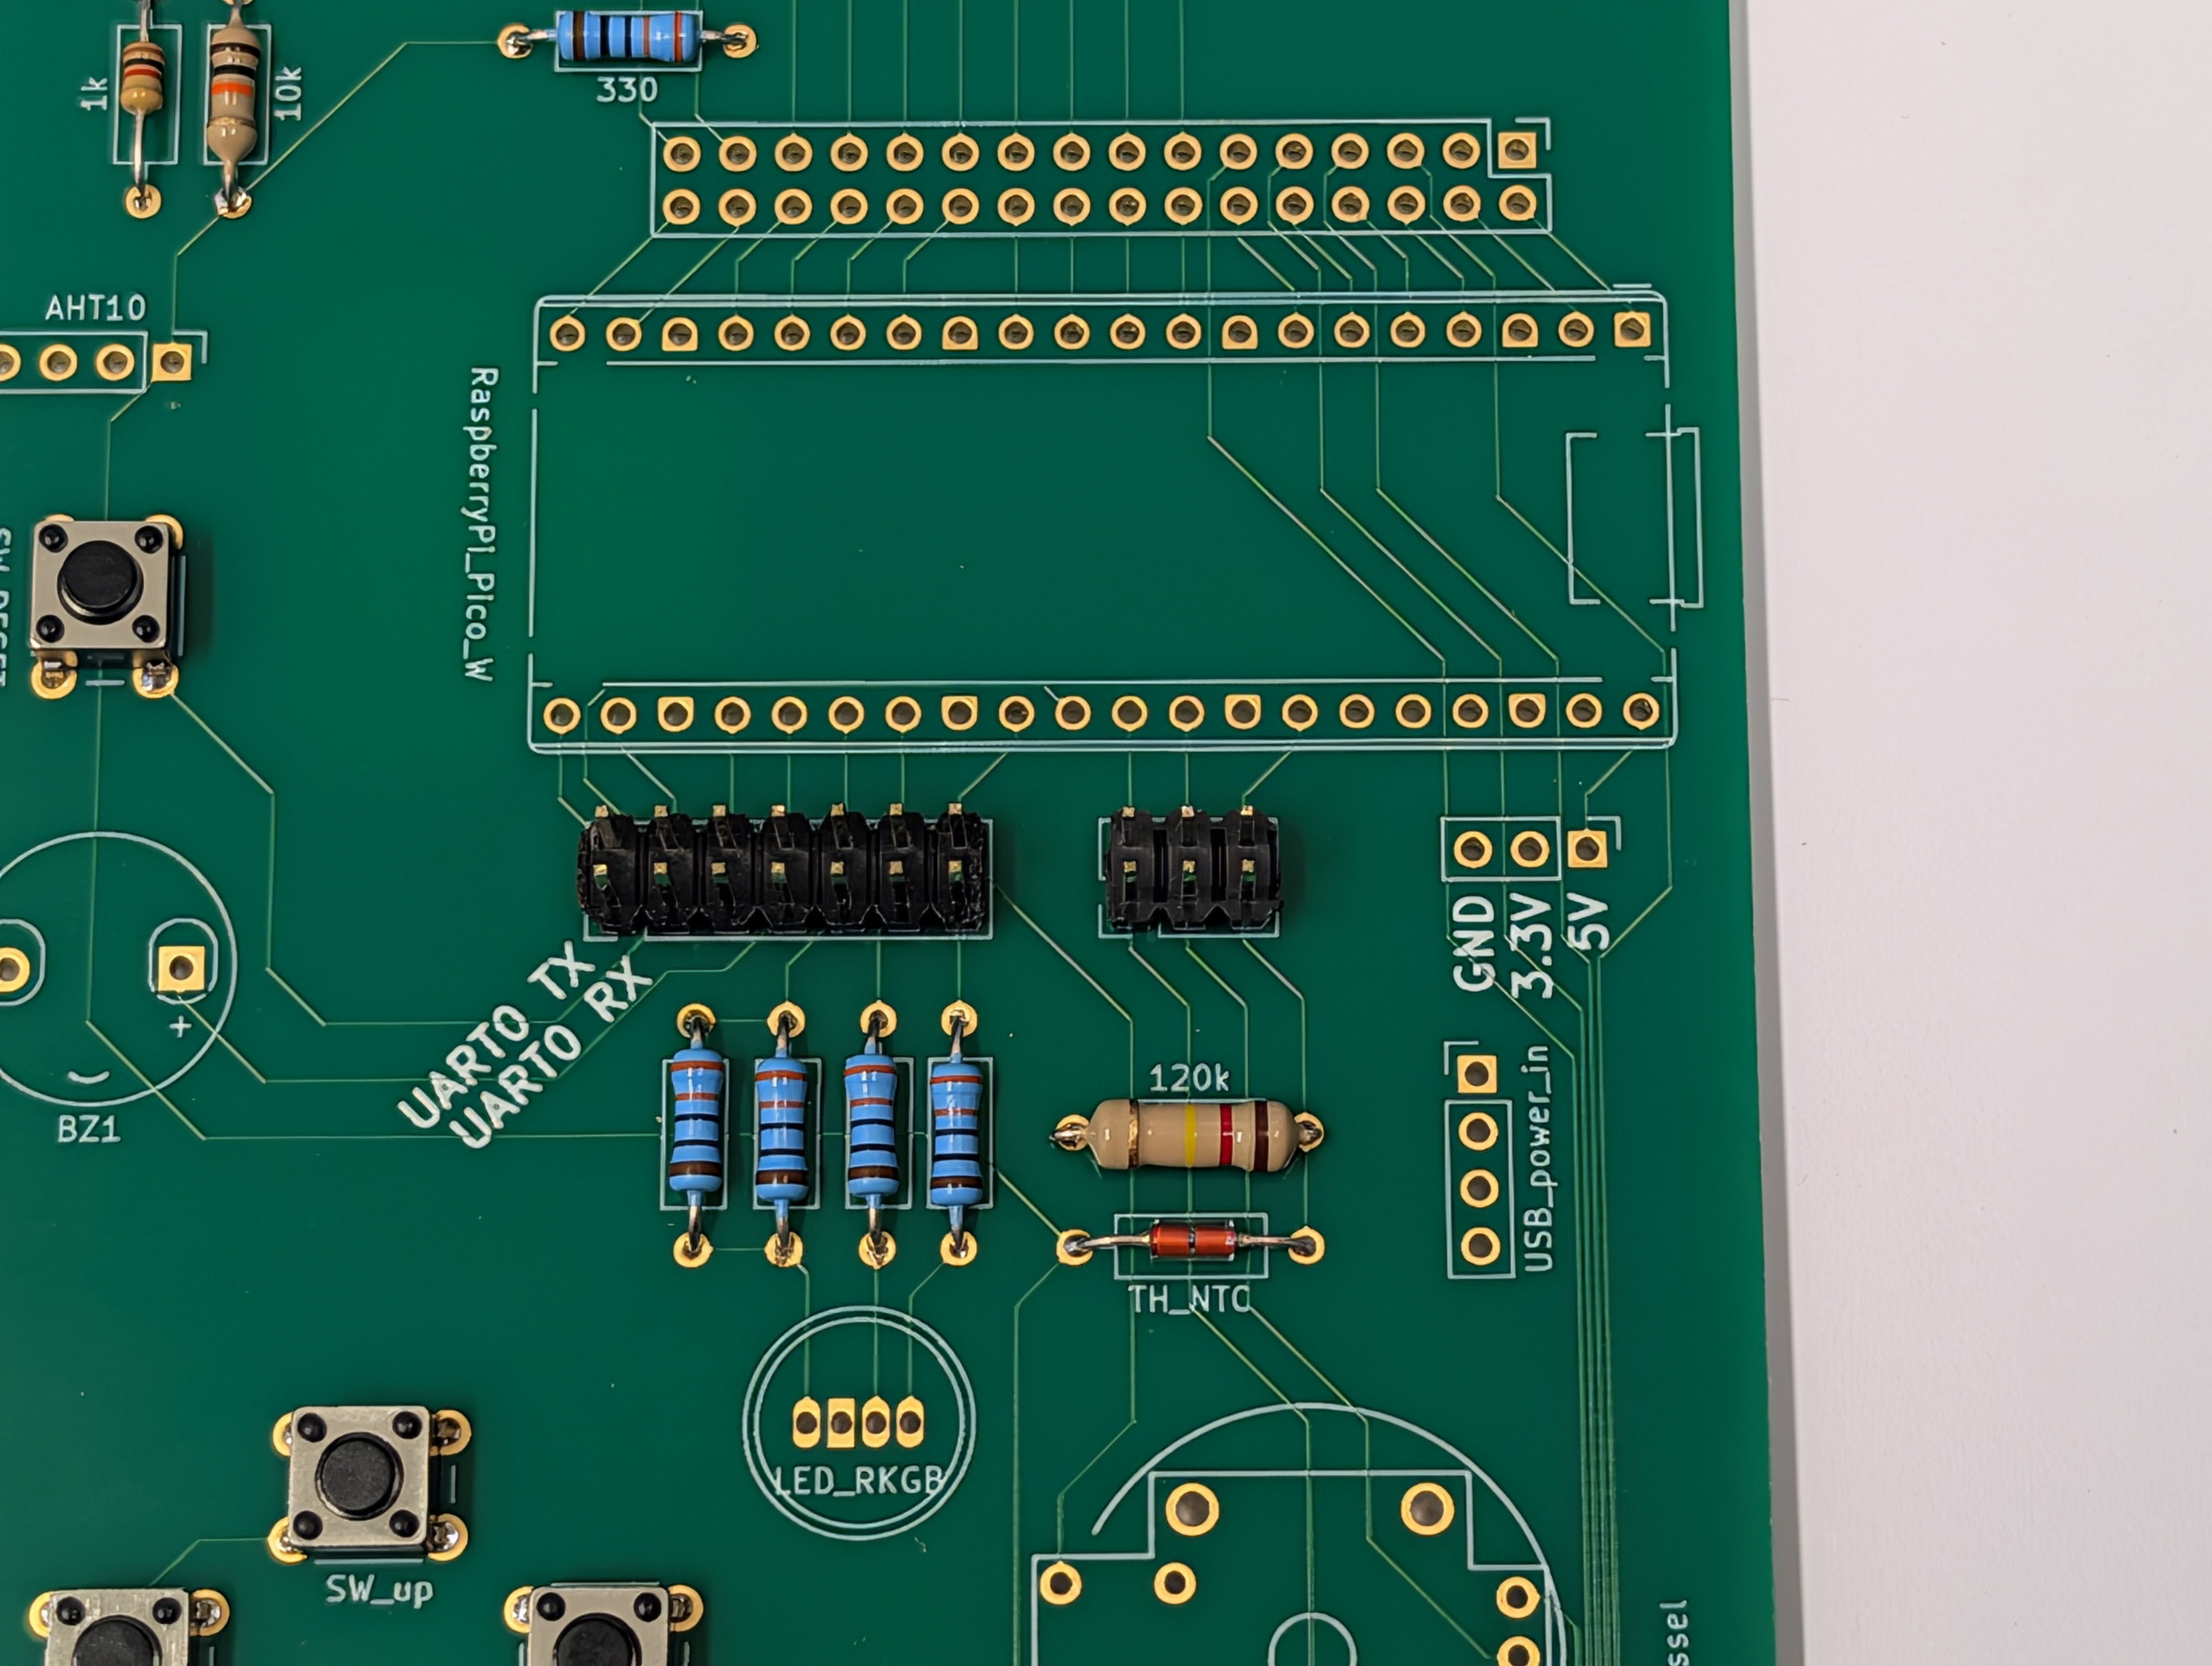
\includegraphics[width=0.75\textwidth]{pictures_of_construction/instruction_step_48.jpg}
\end{figure}

\begin{figure}[H]
    \centering
    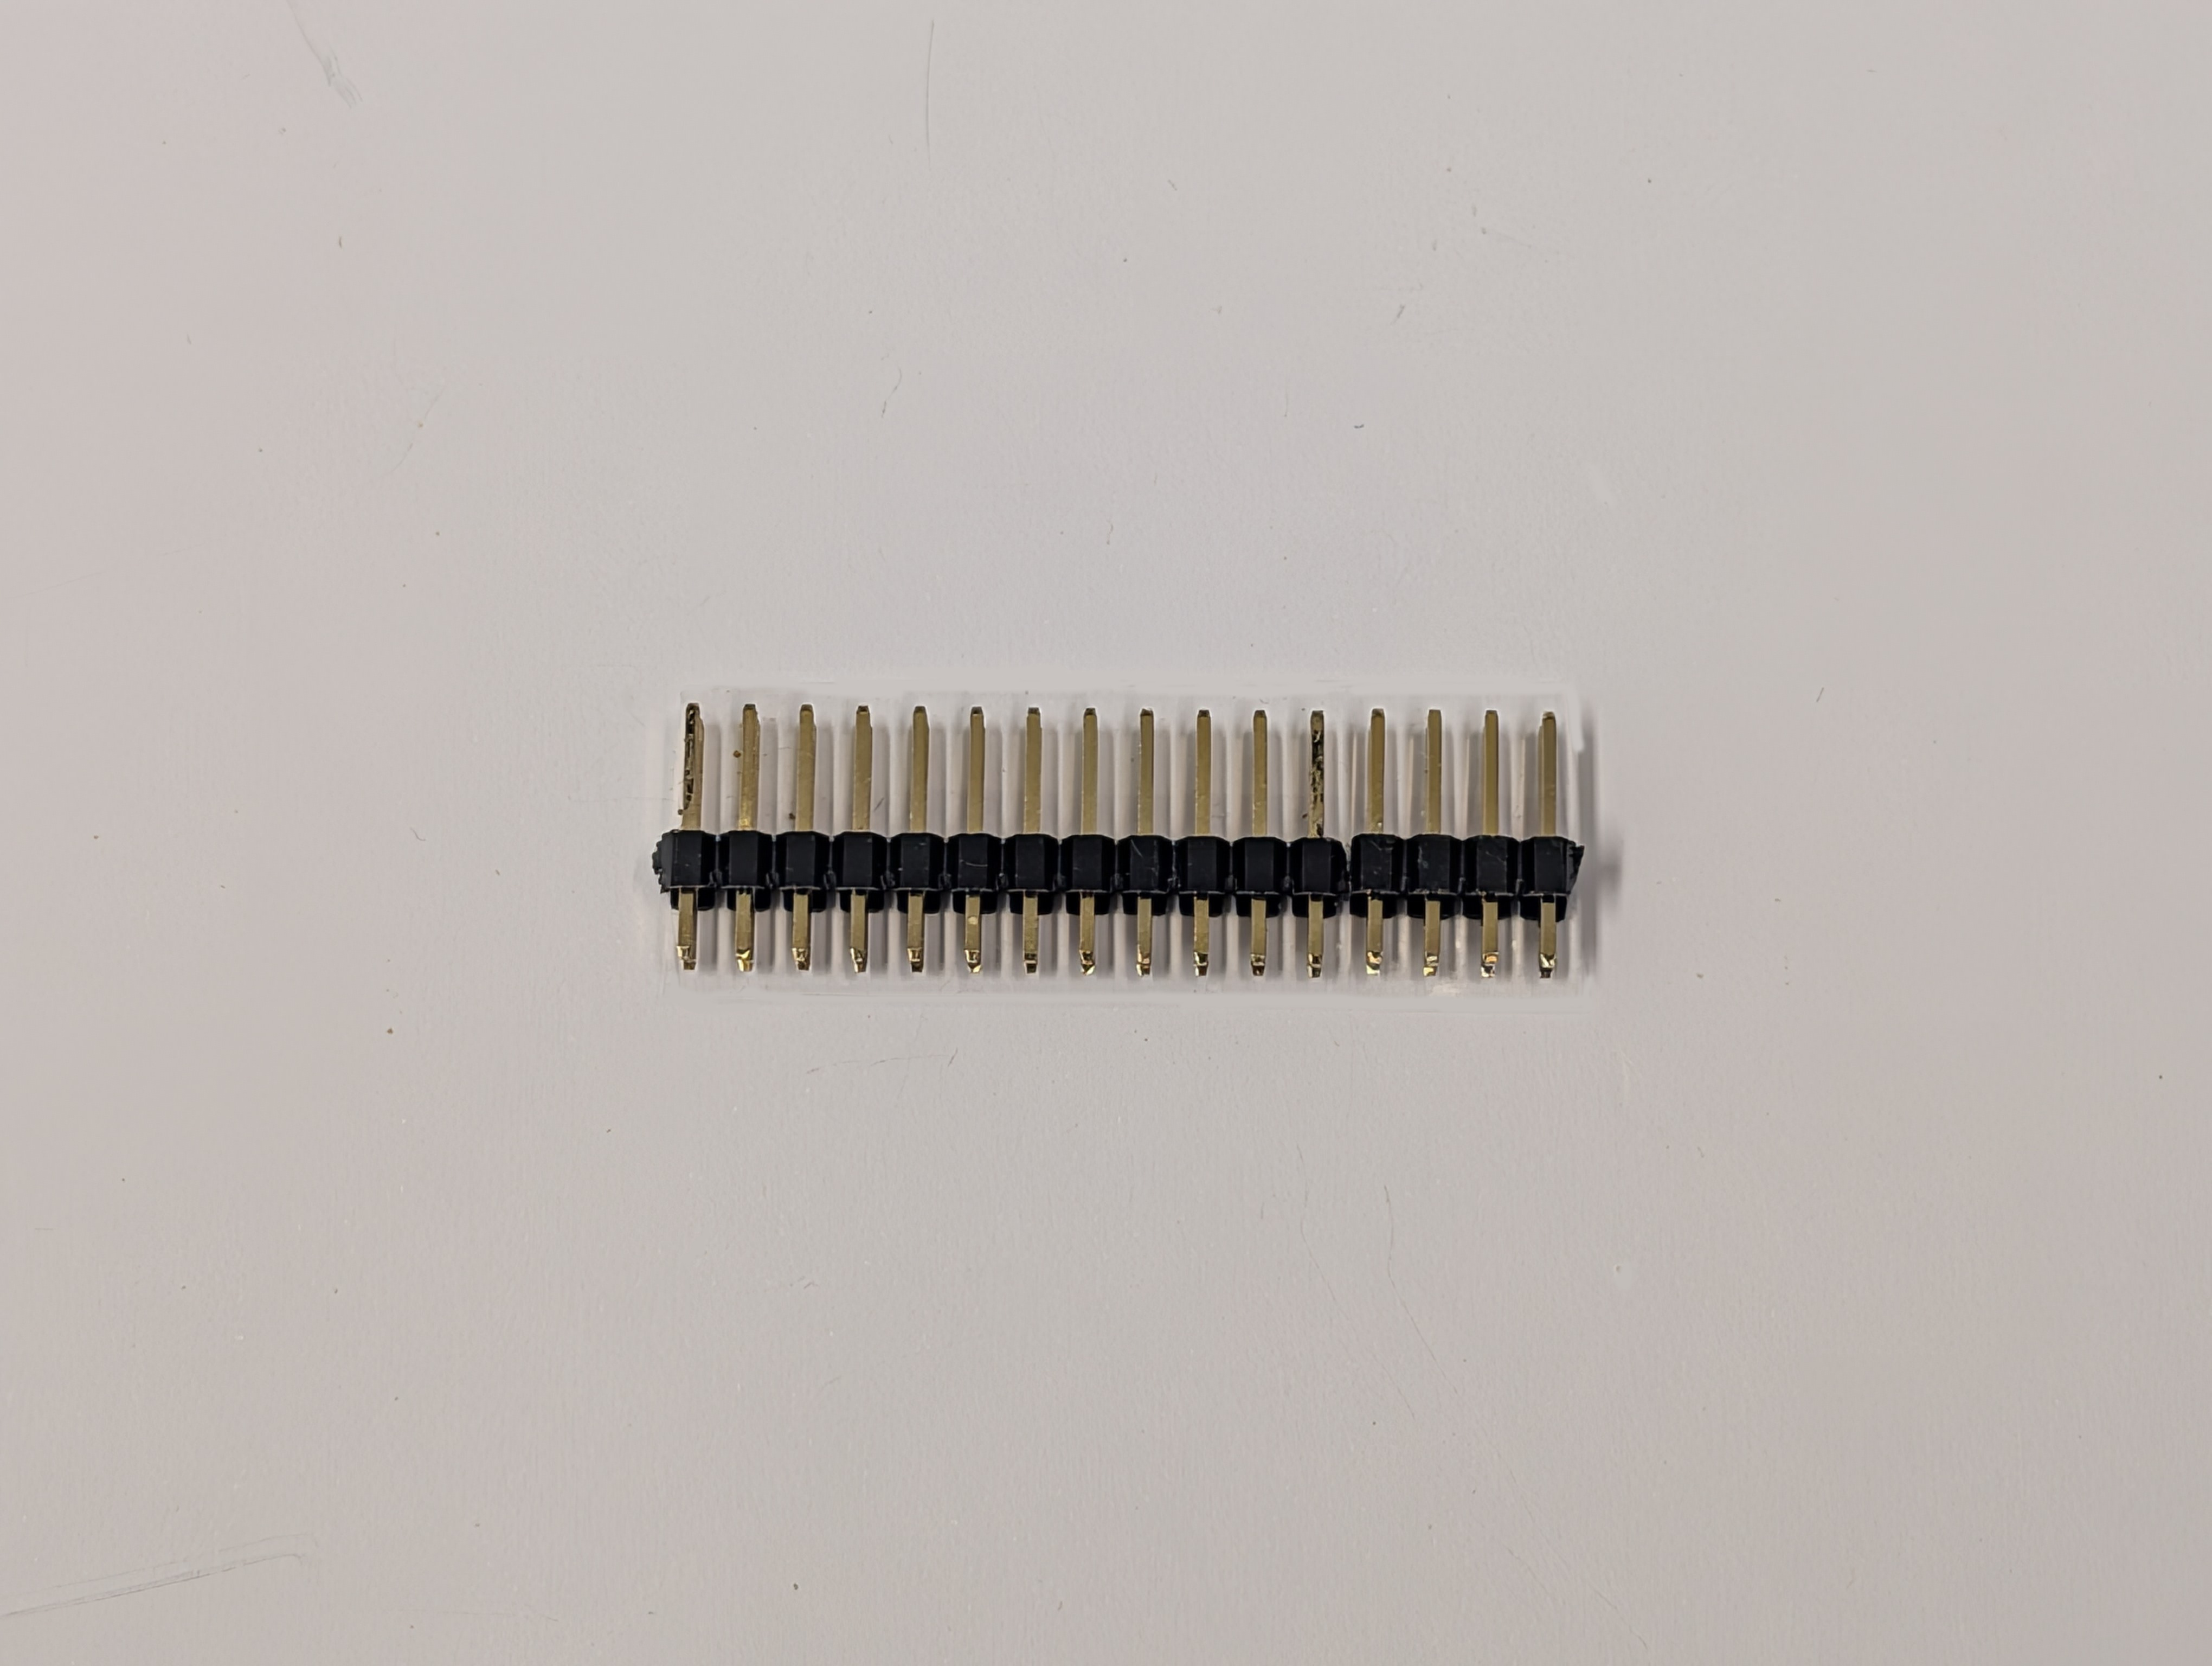
\includegraphics[width=0.75\textwidth]{pictures_of_construction/instruction_step_49.jpg}
\end{figure}

\begin{figure}[H]
    \centering
    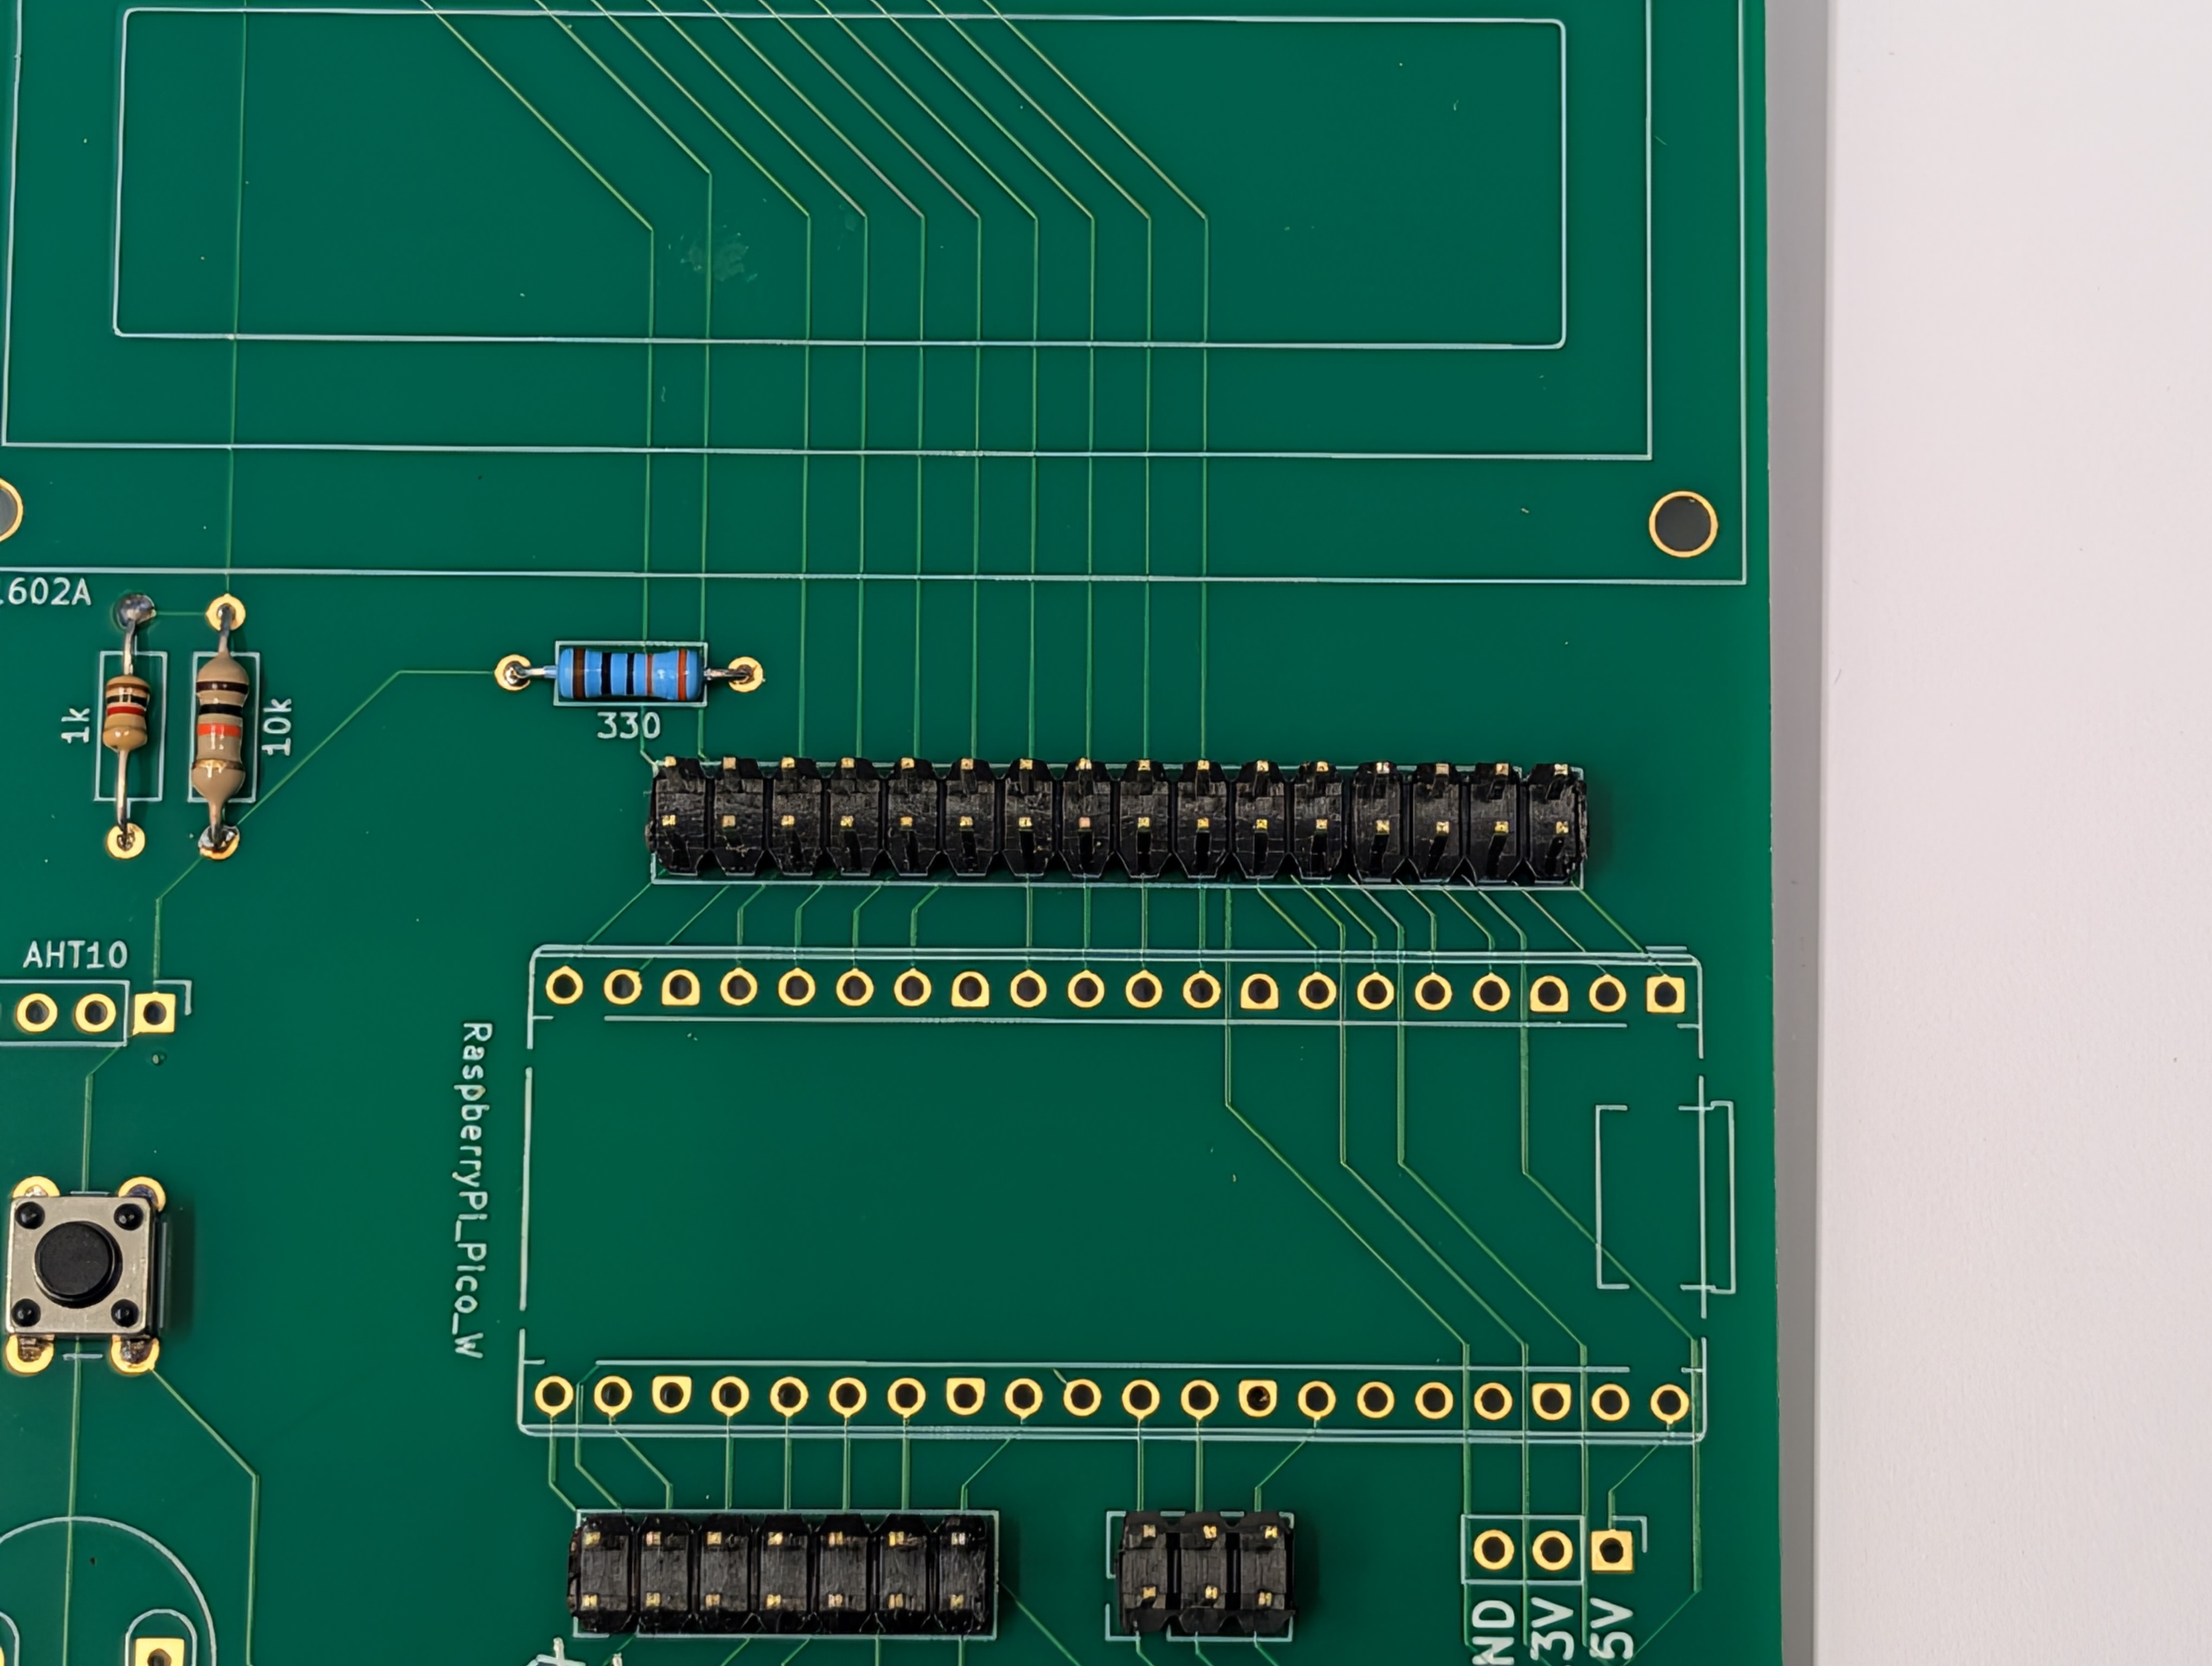
\includegraphics[width=0.75\textwidth]{pictures_of_construction/instruction_step_50.jpg}
\end{figure}

Repeat the previous step for the 2x3 and 2x16 pin headers. Start by soldering one pin, then check and correct the seating, and then solder completely.

\begin{figure}[H]
    \centering
    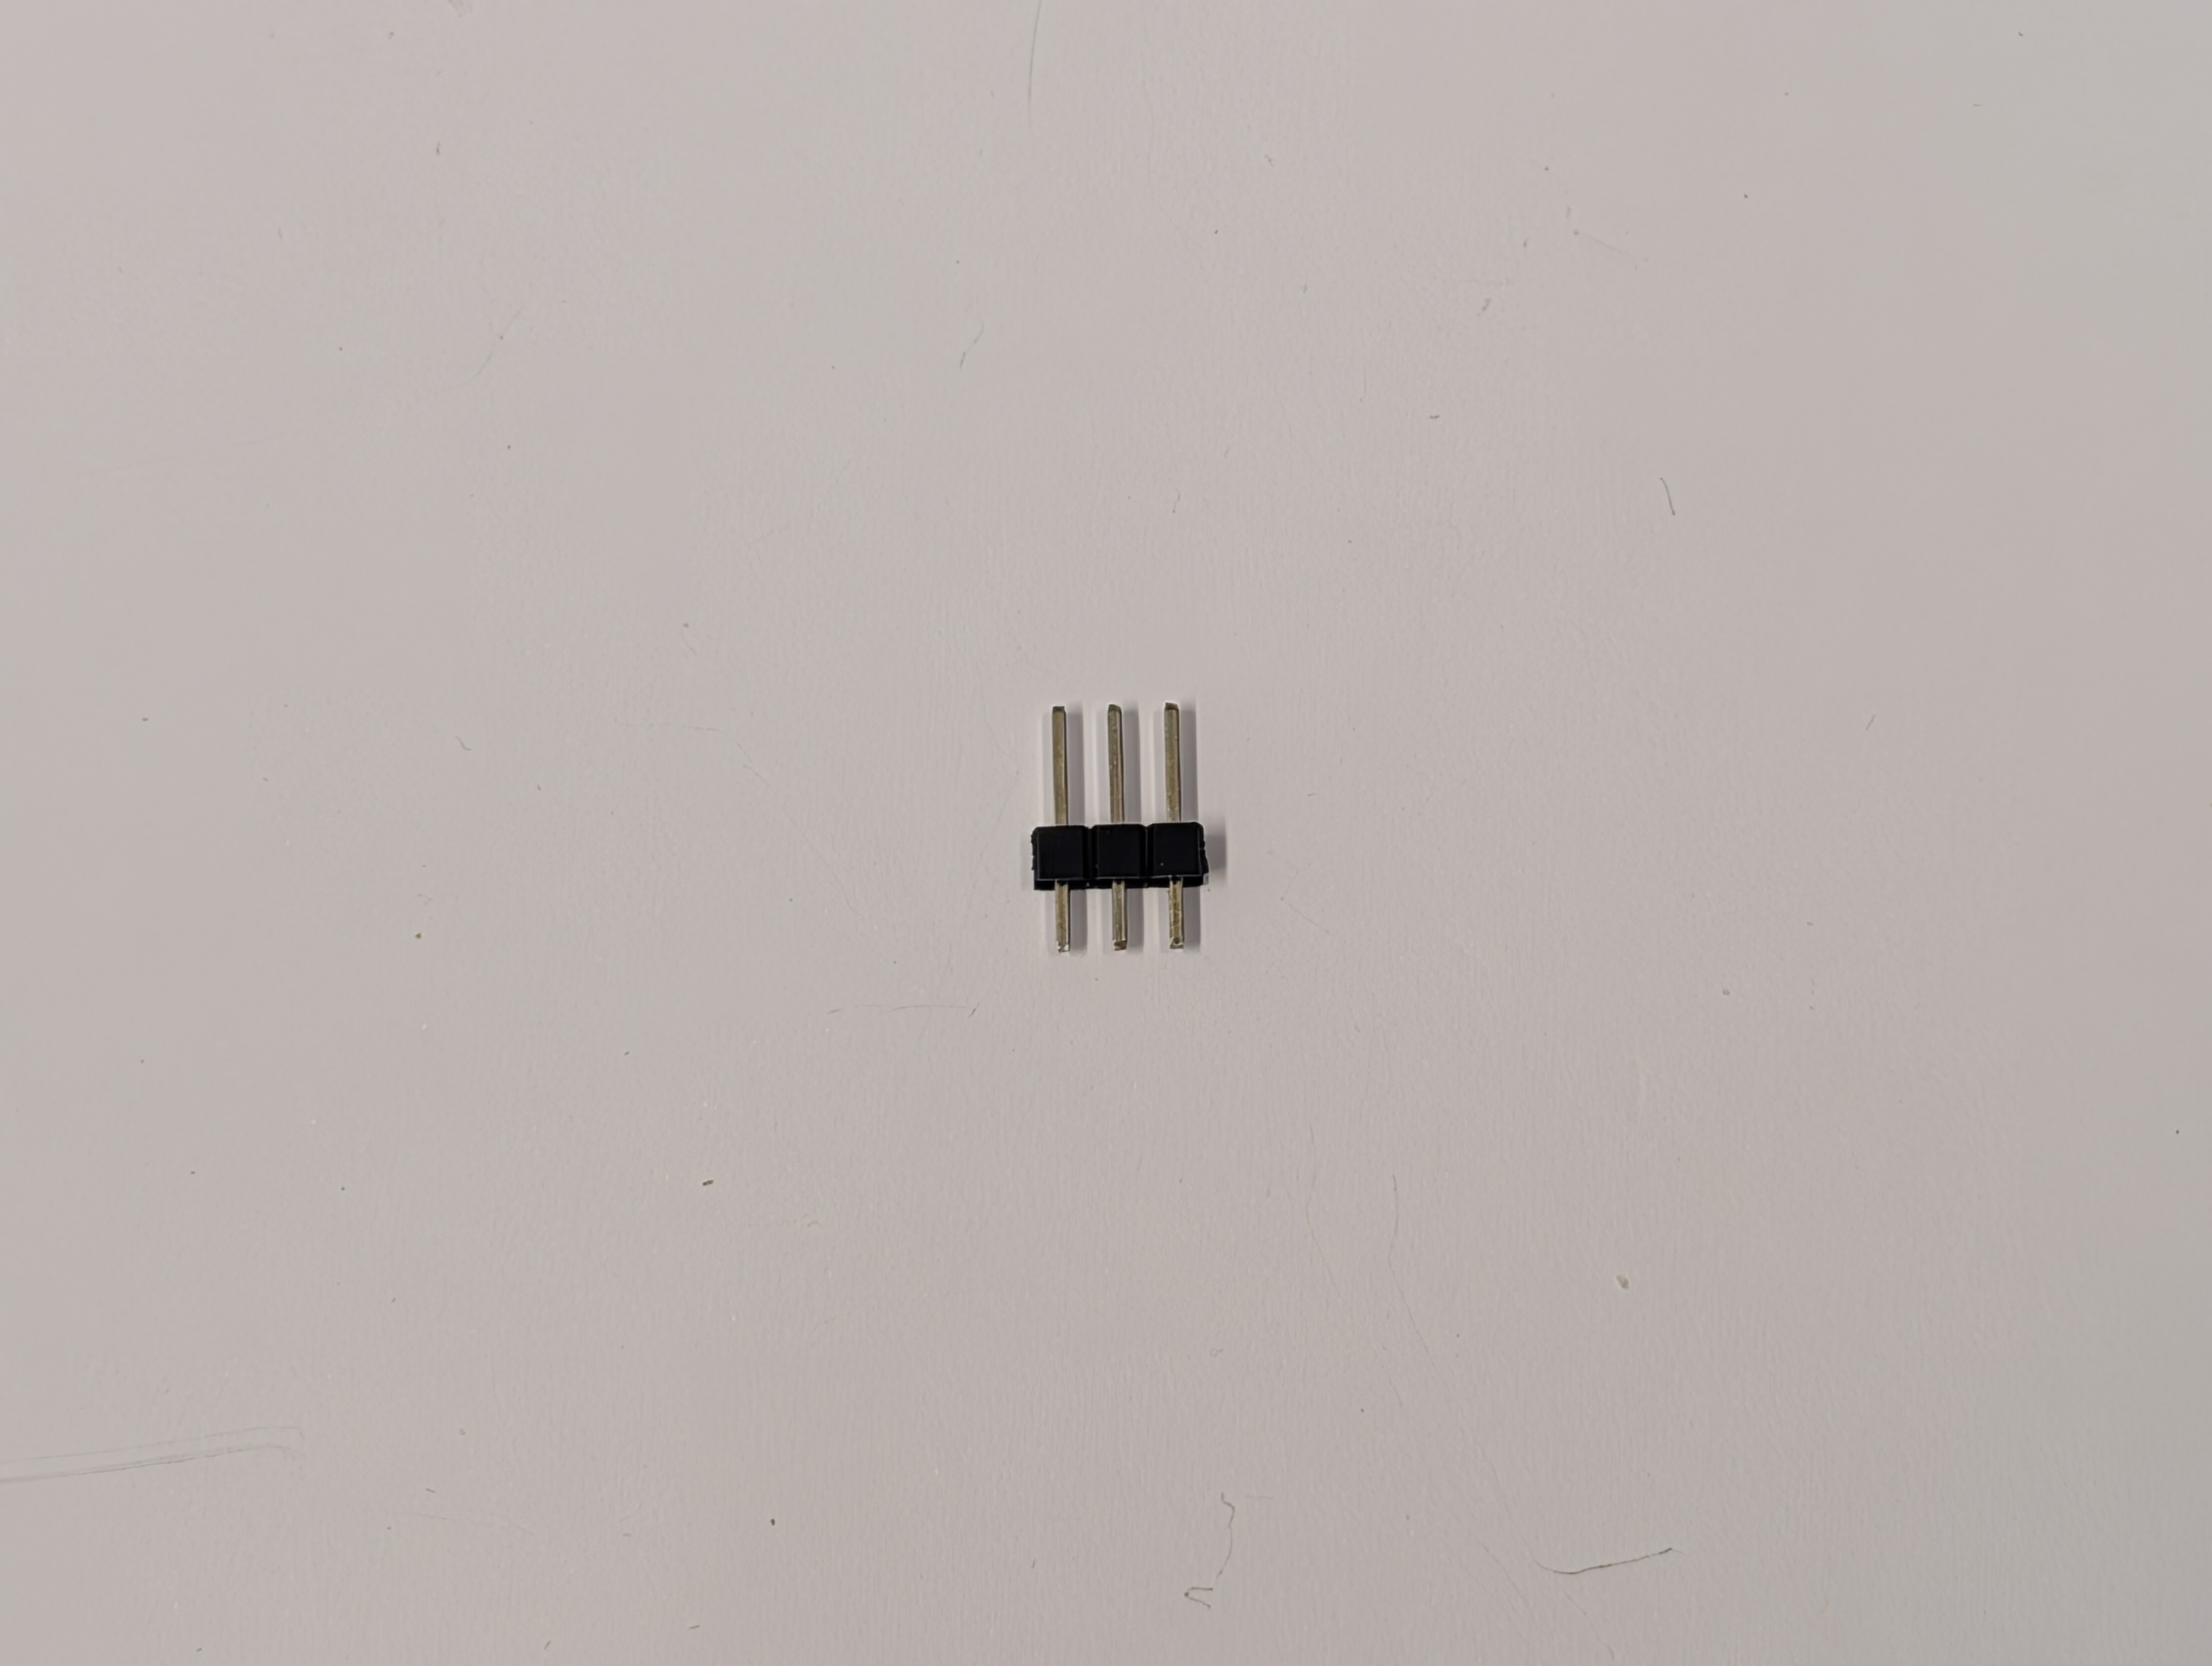
\includegraphics[width=0.75\textwidth]{pictures_of_construction/instruction_step_51.jpg}
\end{figure}

\begin{figure}[H]
    \centering
    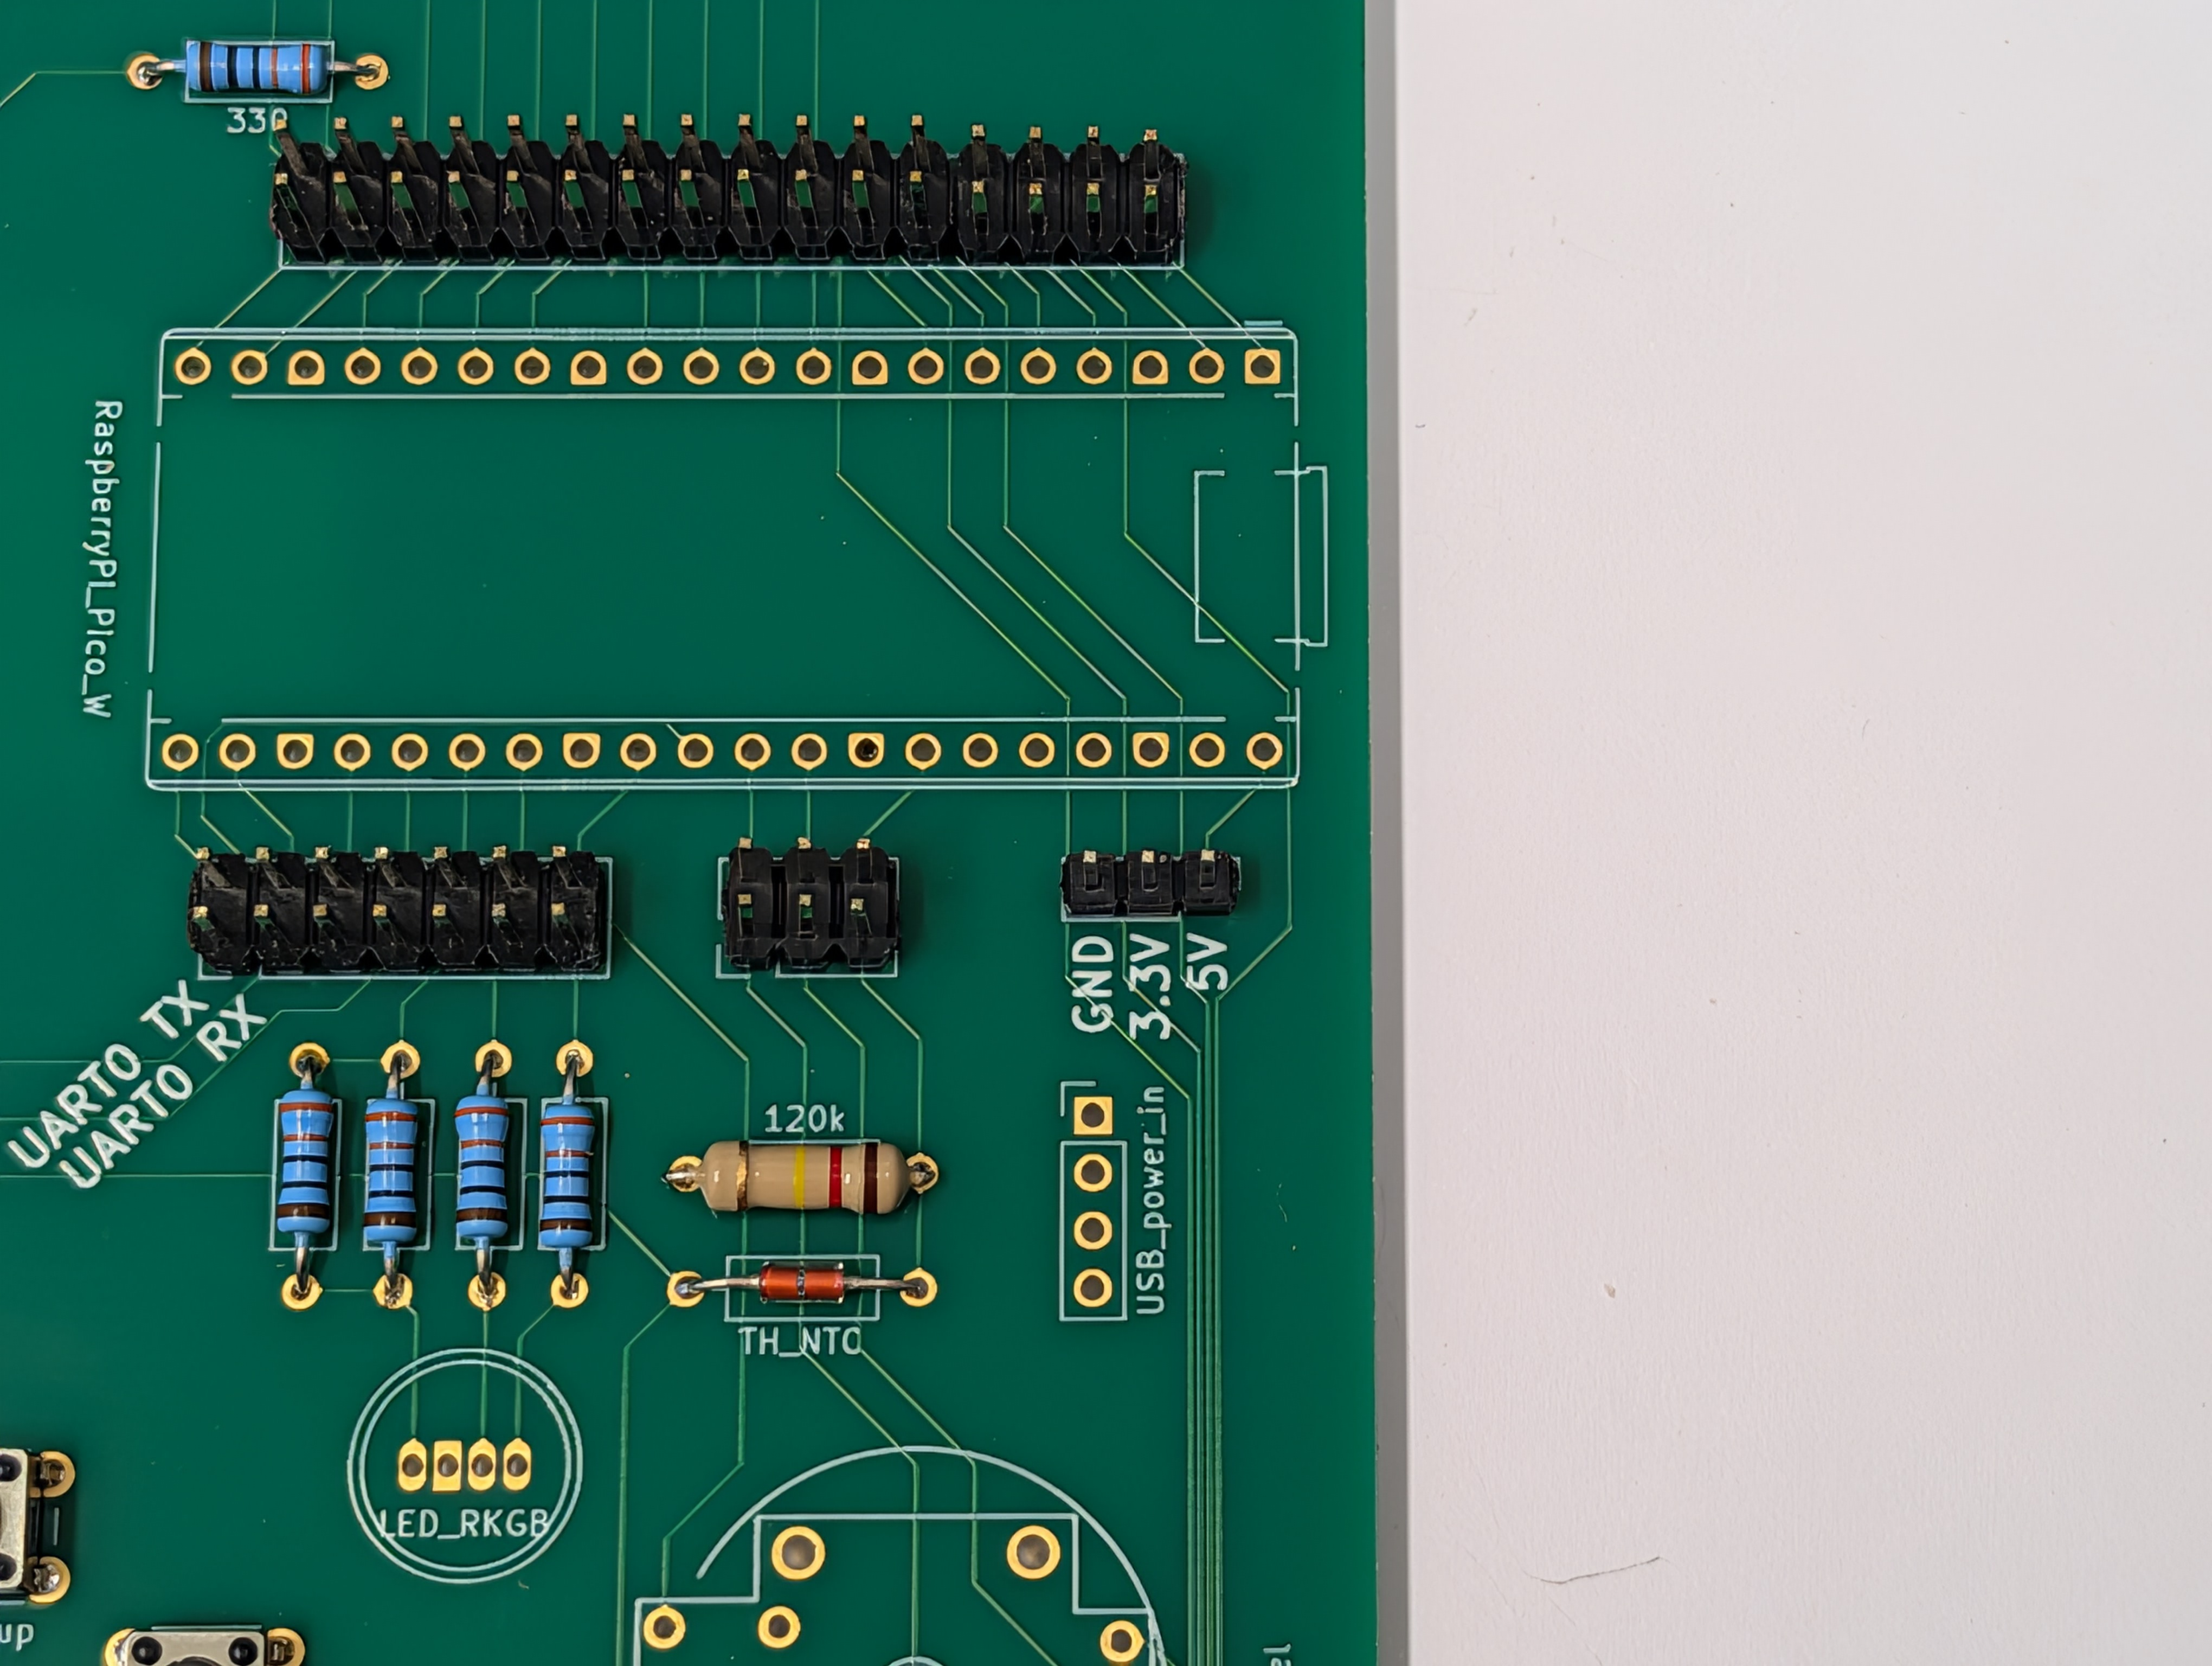
\includegraphics[width=0.75\textwidth]{pictures_of_construction/instruction_step_52.jpg}
\end{figure}

The 1x3 pin header is one of the fiddliest to install. With all the previous practice, you will be able to solder it flush and perpendicular.

\subsection*{Installation of the USB-C breakout board}

\begin{figure}[H]
    \centering
    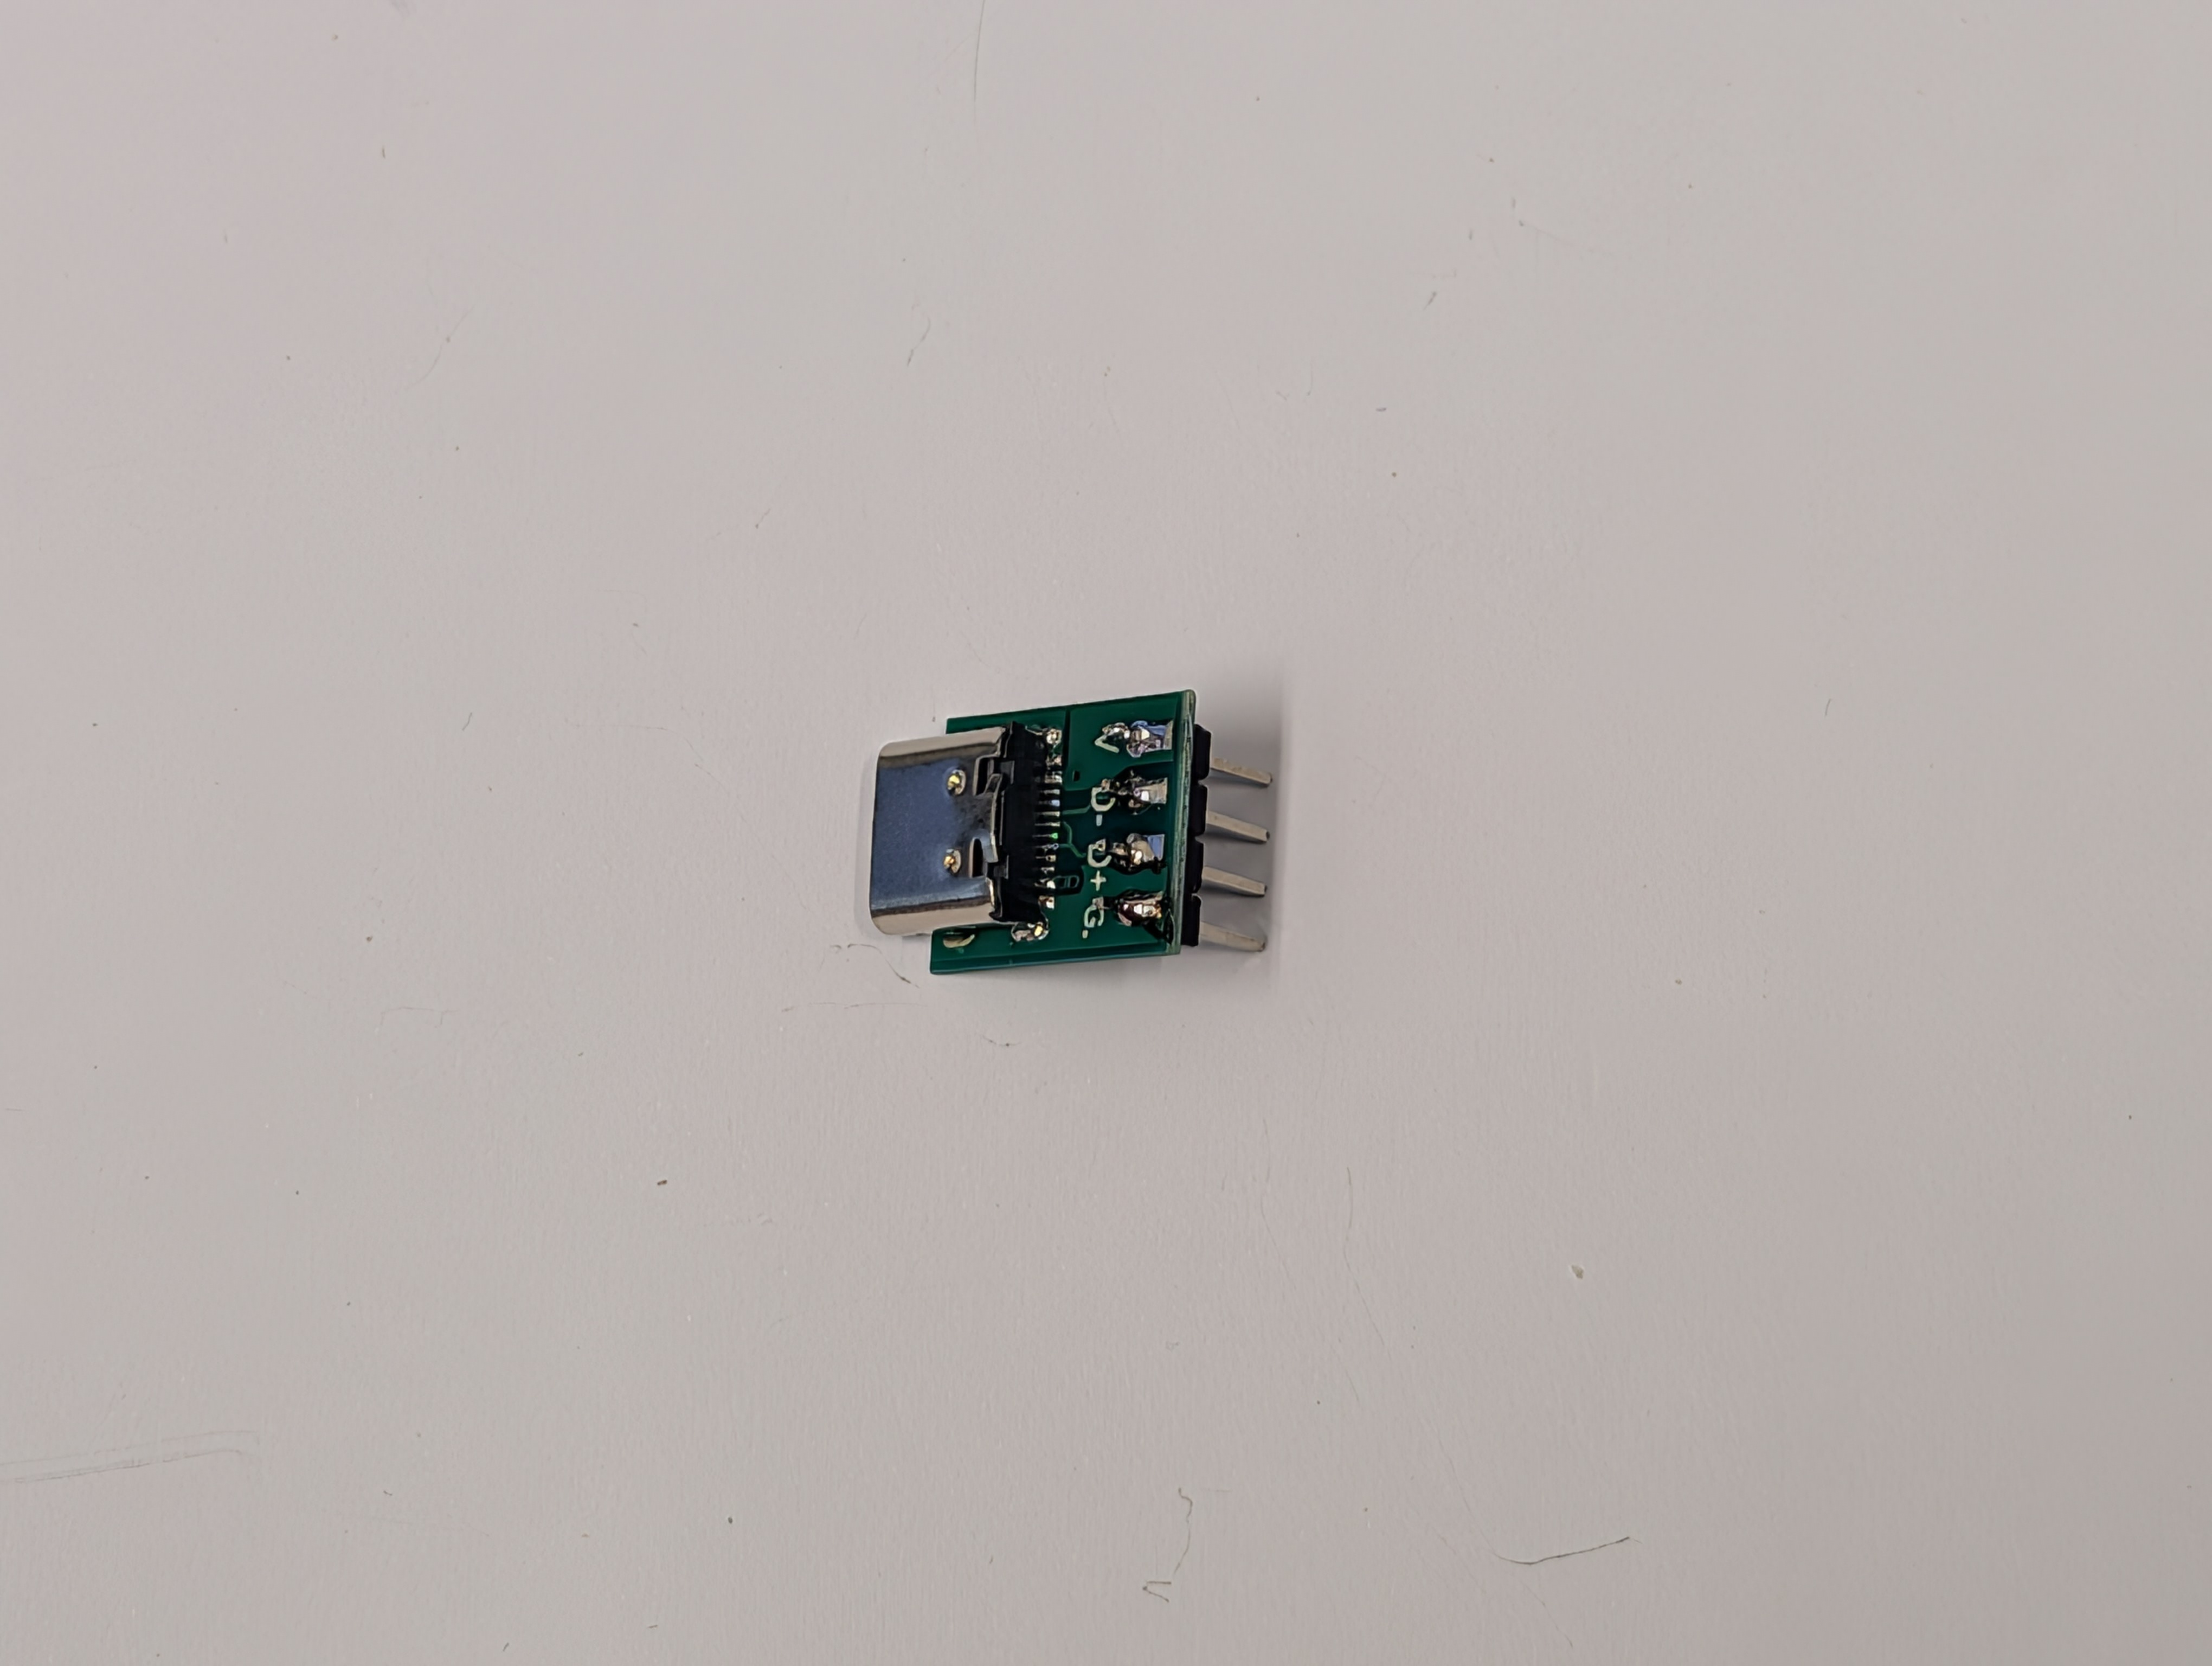
\includegraphics[width=0.75\textwidth]{pictures_of_construction/instruction_step_53.jpg}
\end{figure}

\begin{figure}[H]
    \centering
    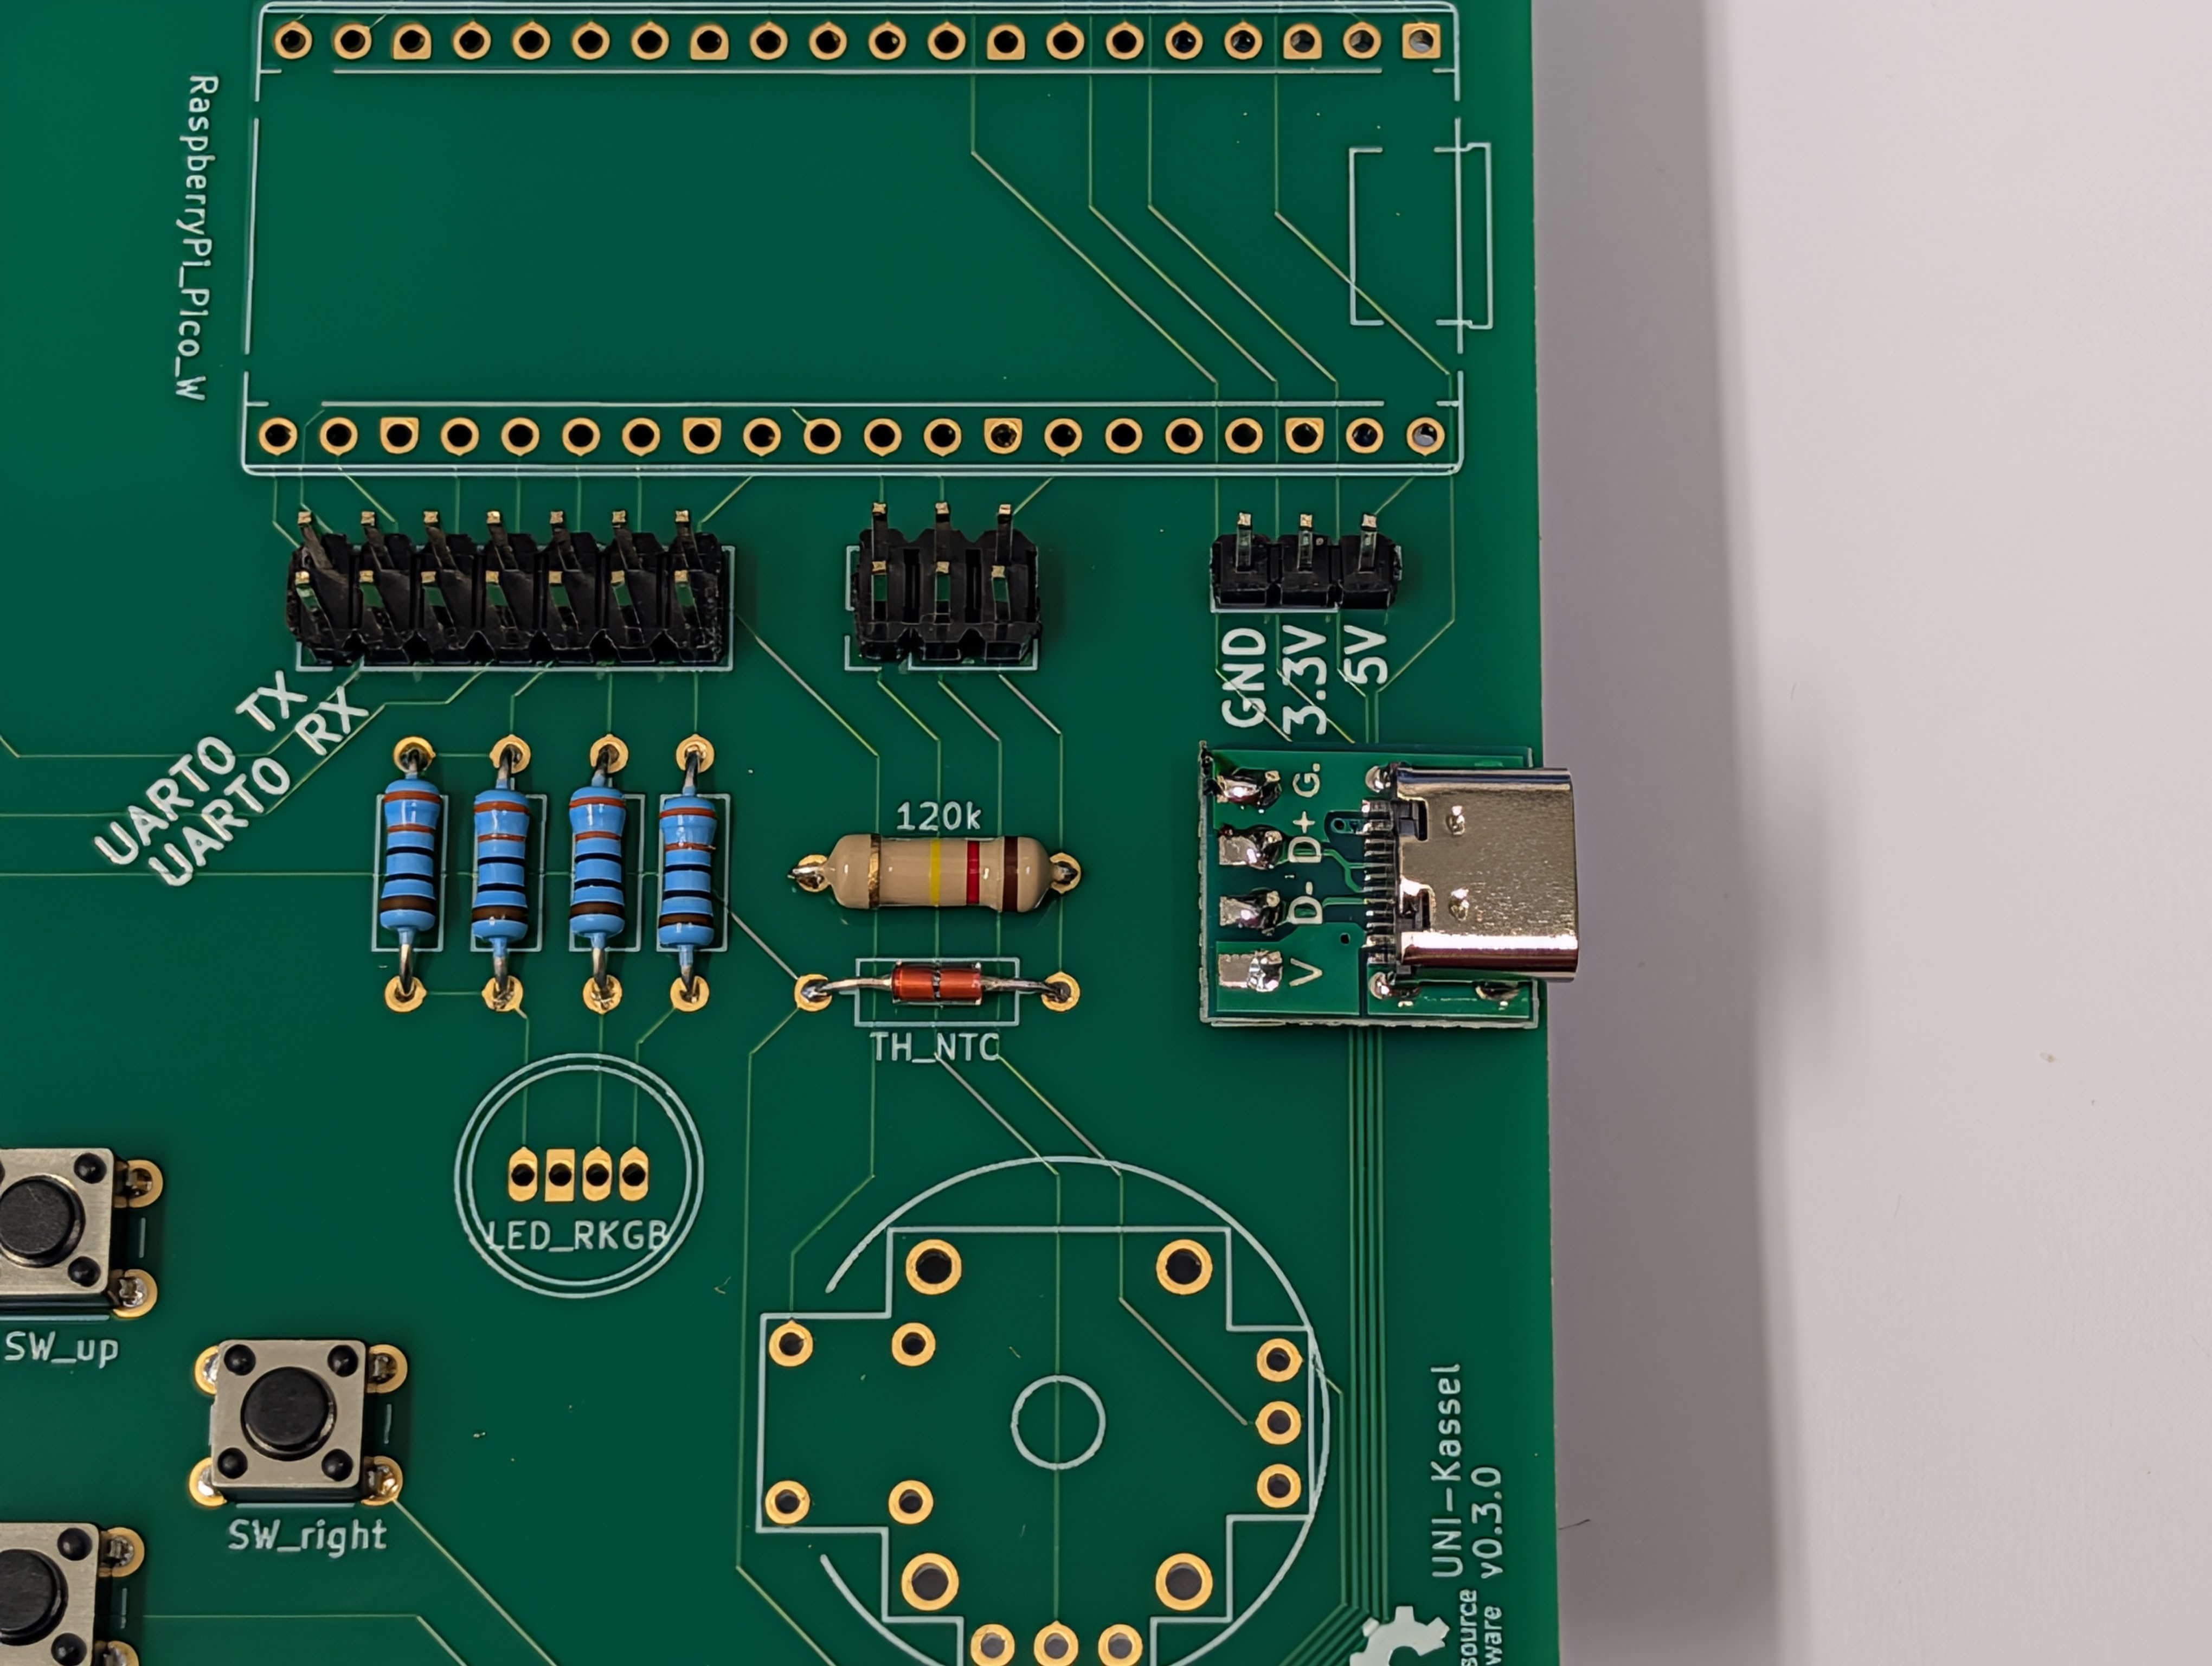
\includegraphics[width=0.75\textwidth]{pictures_of_construction/instruction_step_54.jpg}
\end{figure}

\begin{figure}[H]
    \centering
    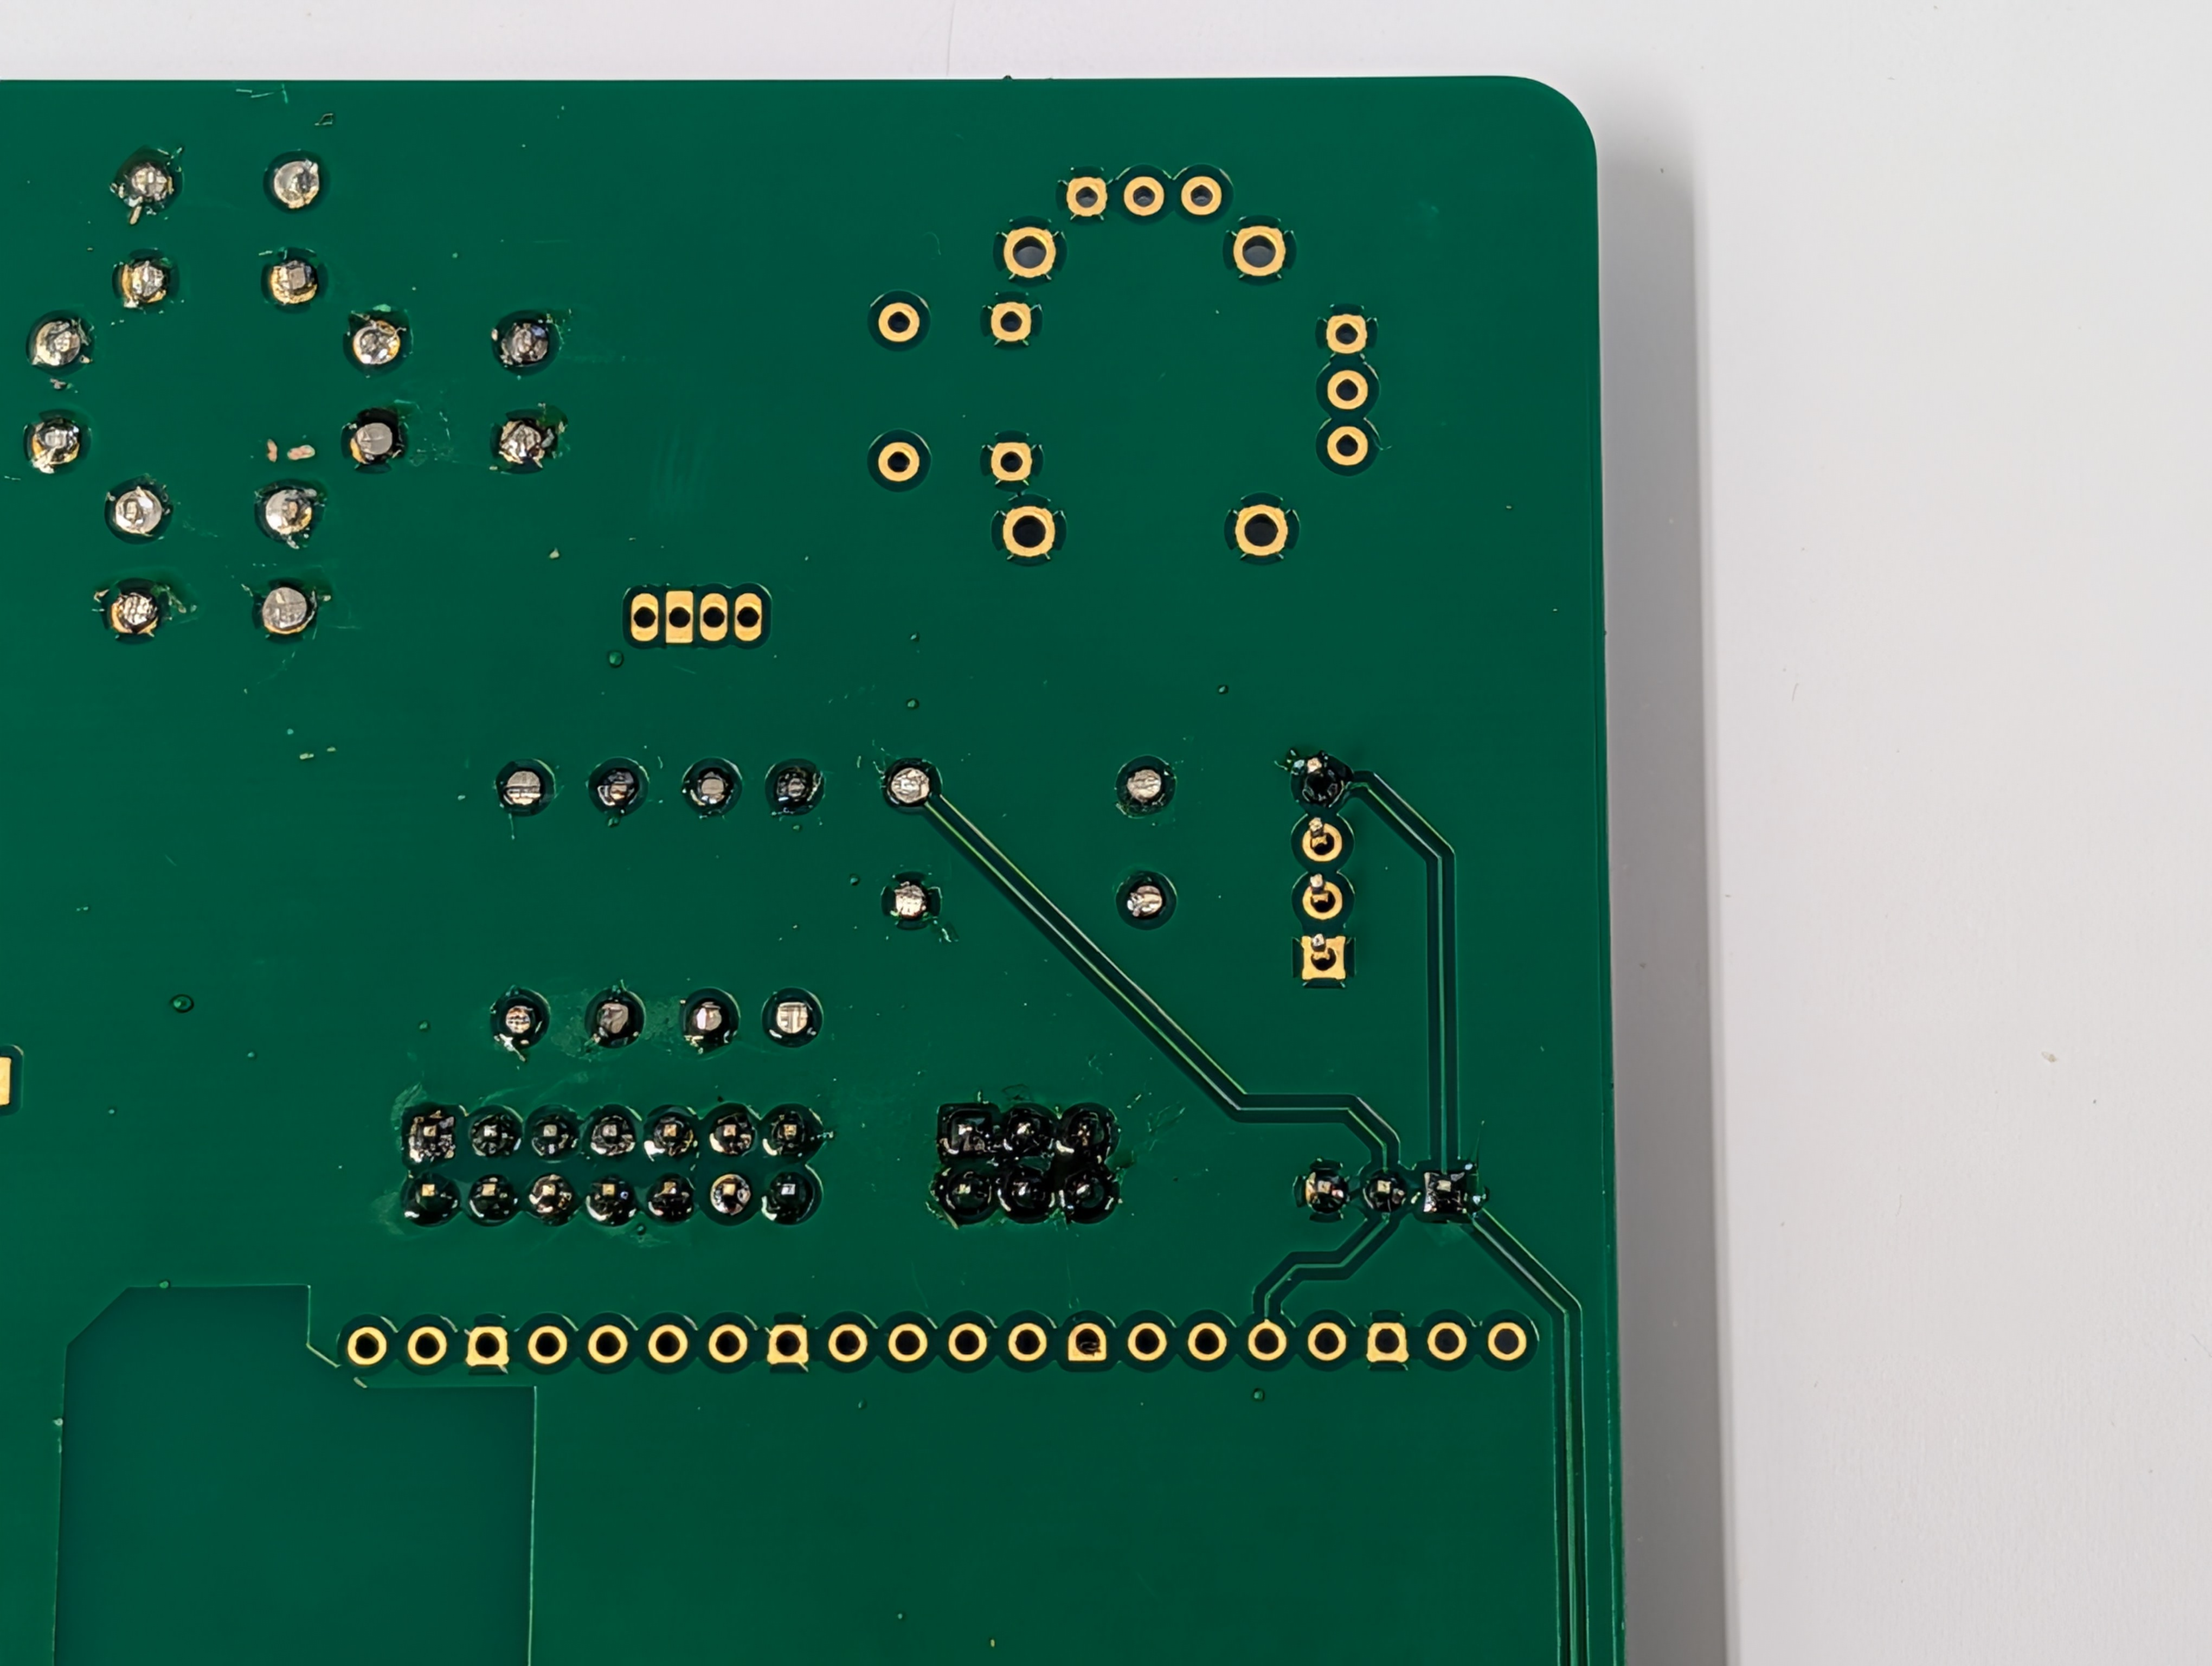
\includegraphics[width=0.75\textwidth]{pictures_of_construction/instruction_step_55.jpg}
\end{figure}

\begin{figure}[H]
    \centering
    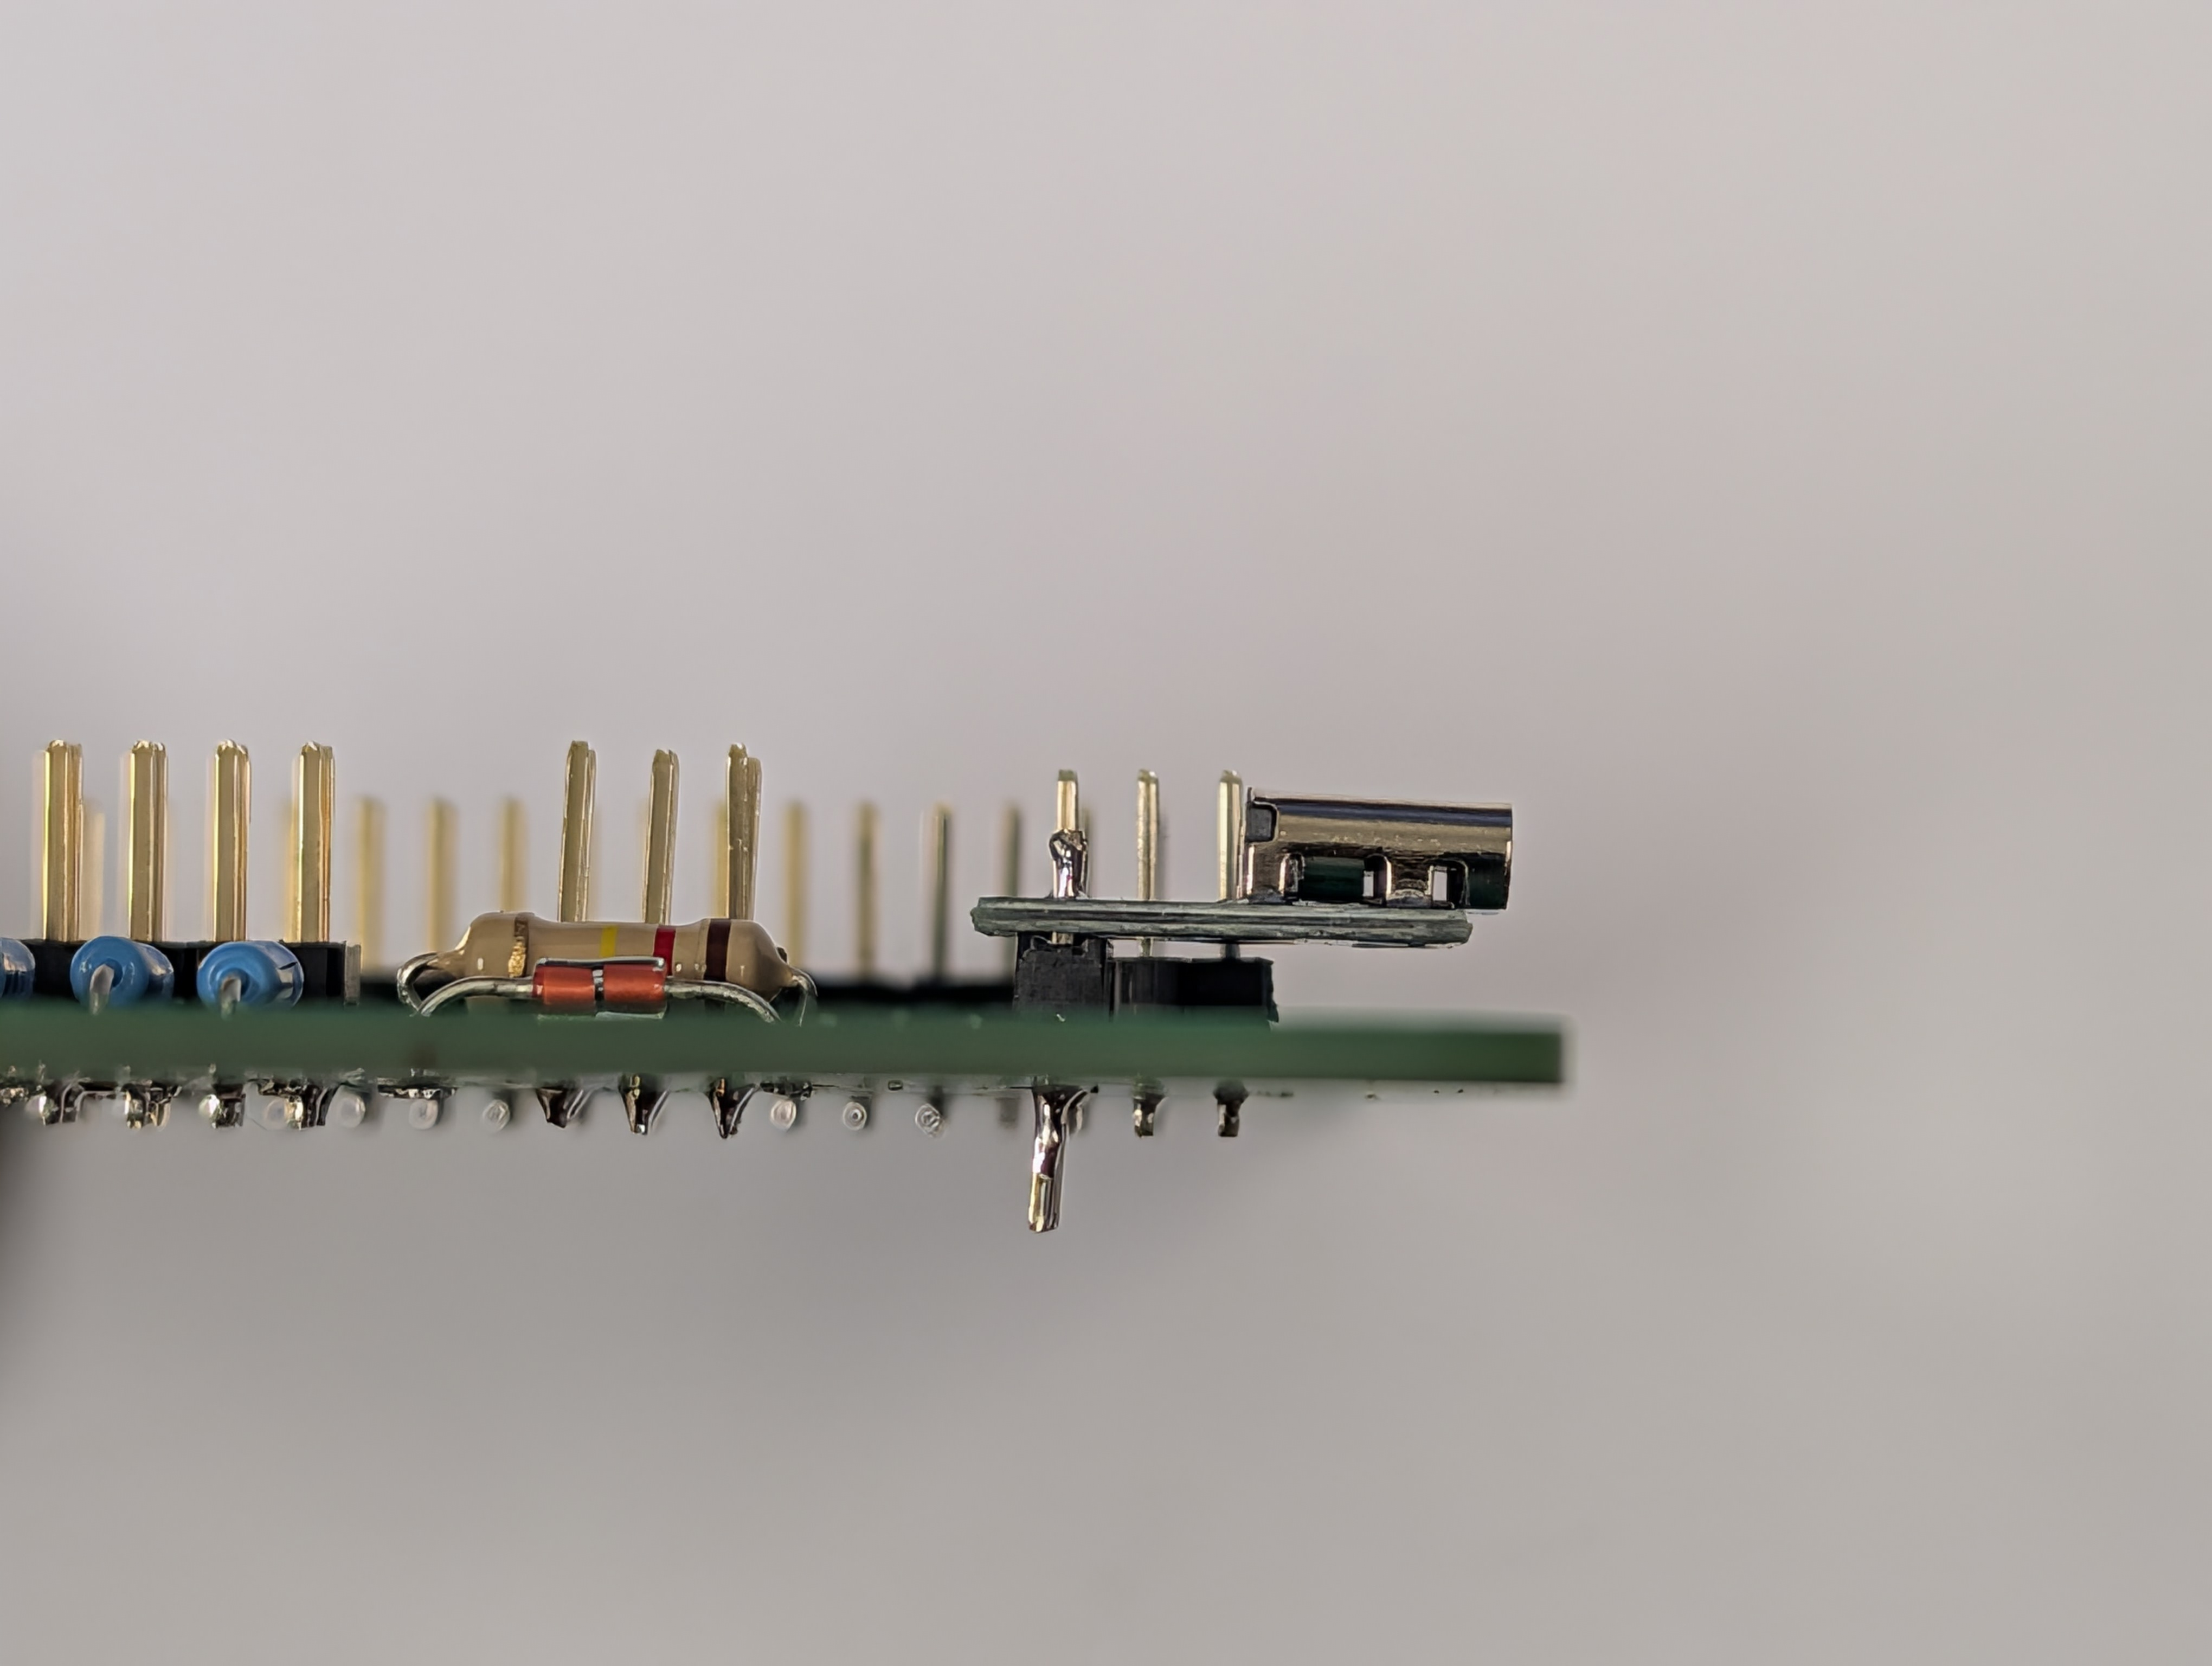
\includegraphics[width=0.75\textwidth]{pictures_of_construction/instruction_step_56.jpg}
\end{figure}

Now we can solder the USB-C breakout board. After placing it into position (right side of the Buzzerino PCB, facing outwards, the USB port should be fully visible), solder one pin. Then check for alignment; it should be parallel to the Buzzerino PCB. Then solder it completely.

\textbf{WARNING:} The pins of the USB-C breakout board, the AHT10 temperature sensor, and the 1602A LCD display are too hard for electronics side cutters. Use larger wire cutters as provided.

\subsection*{Installation of the AHT10 digital temperature sensor}

\begin{figure}[H]
    \centering
    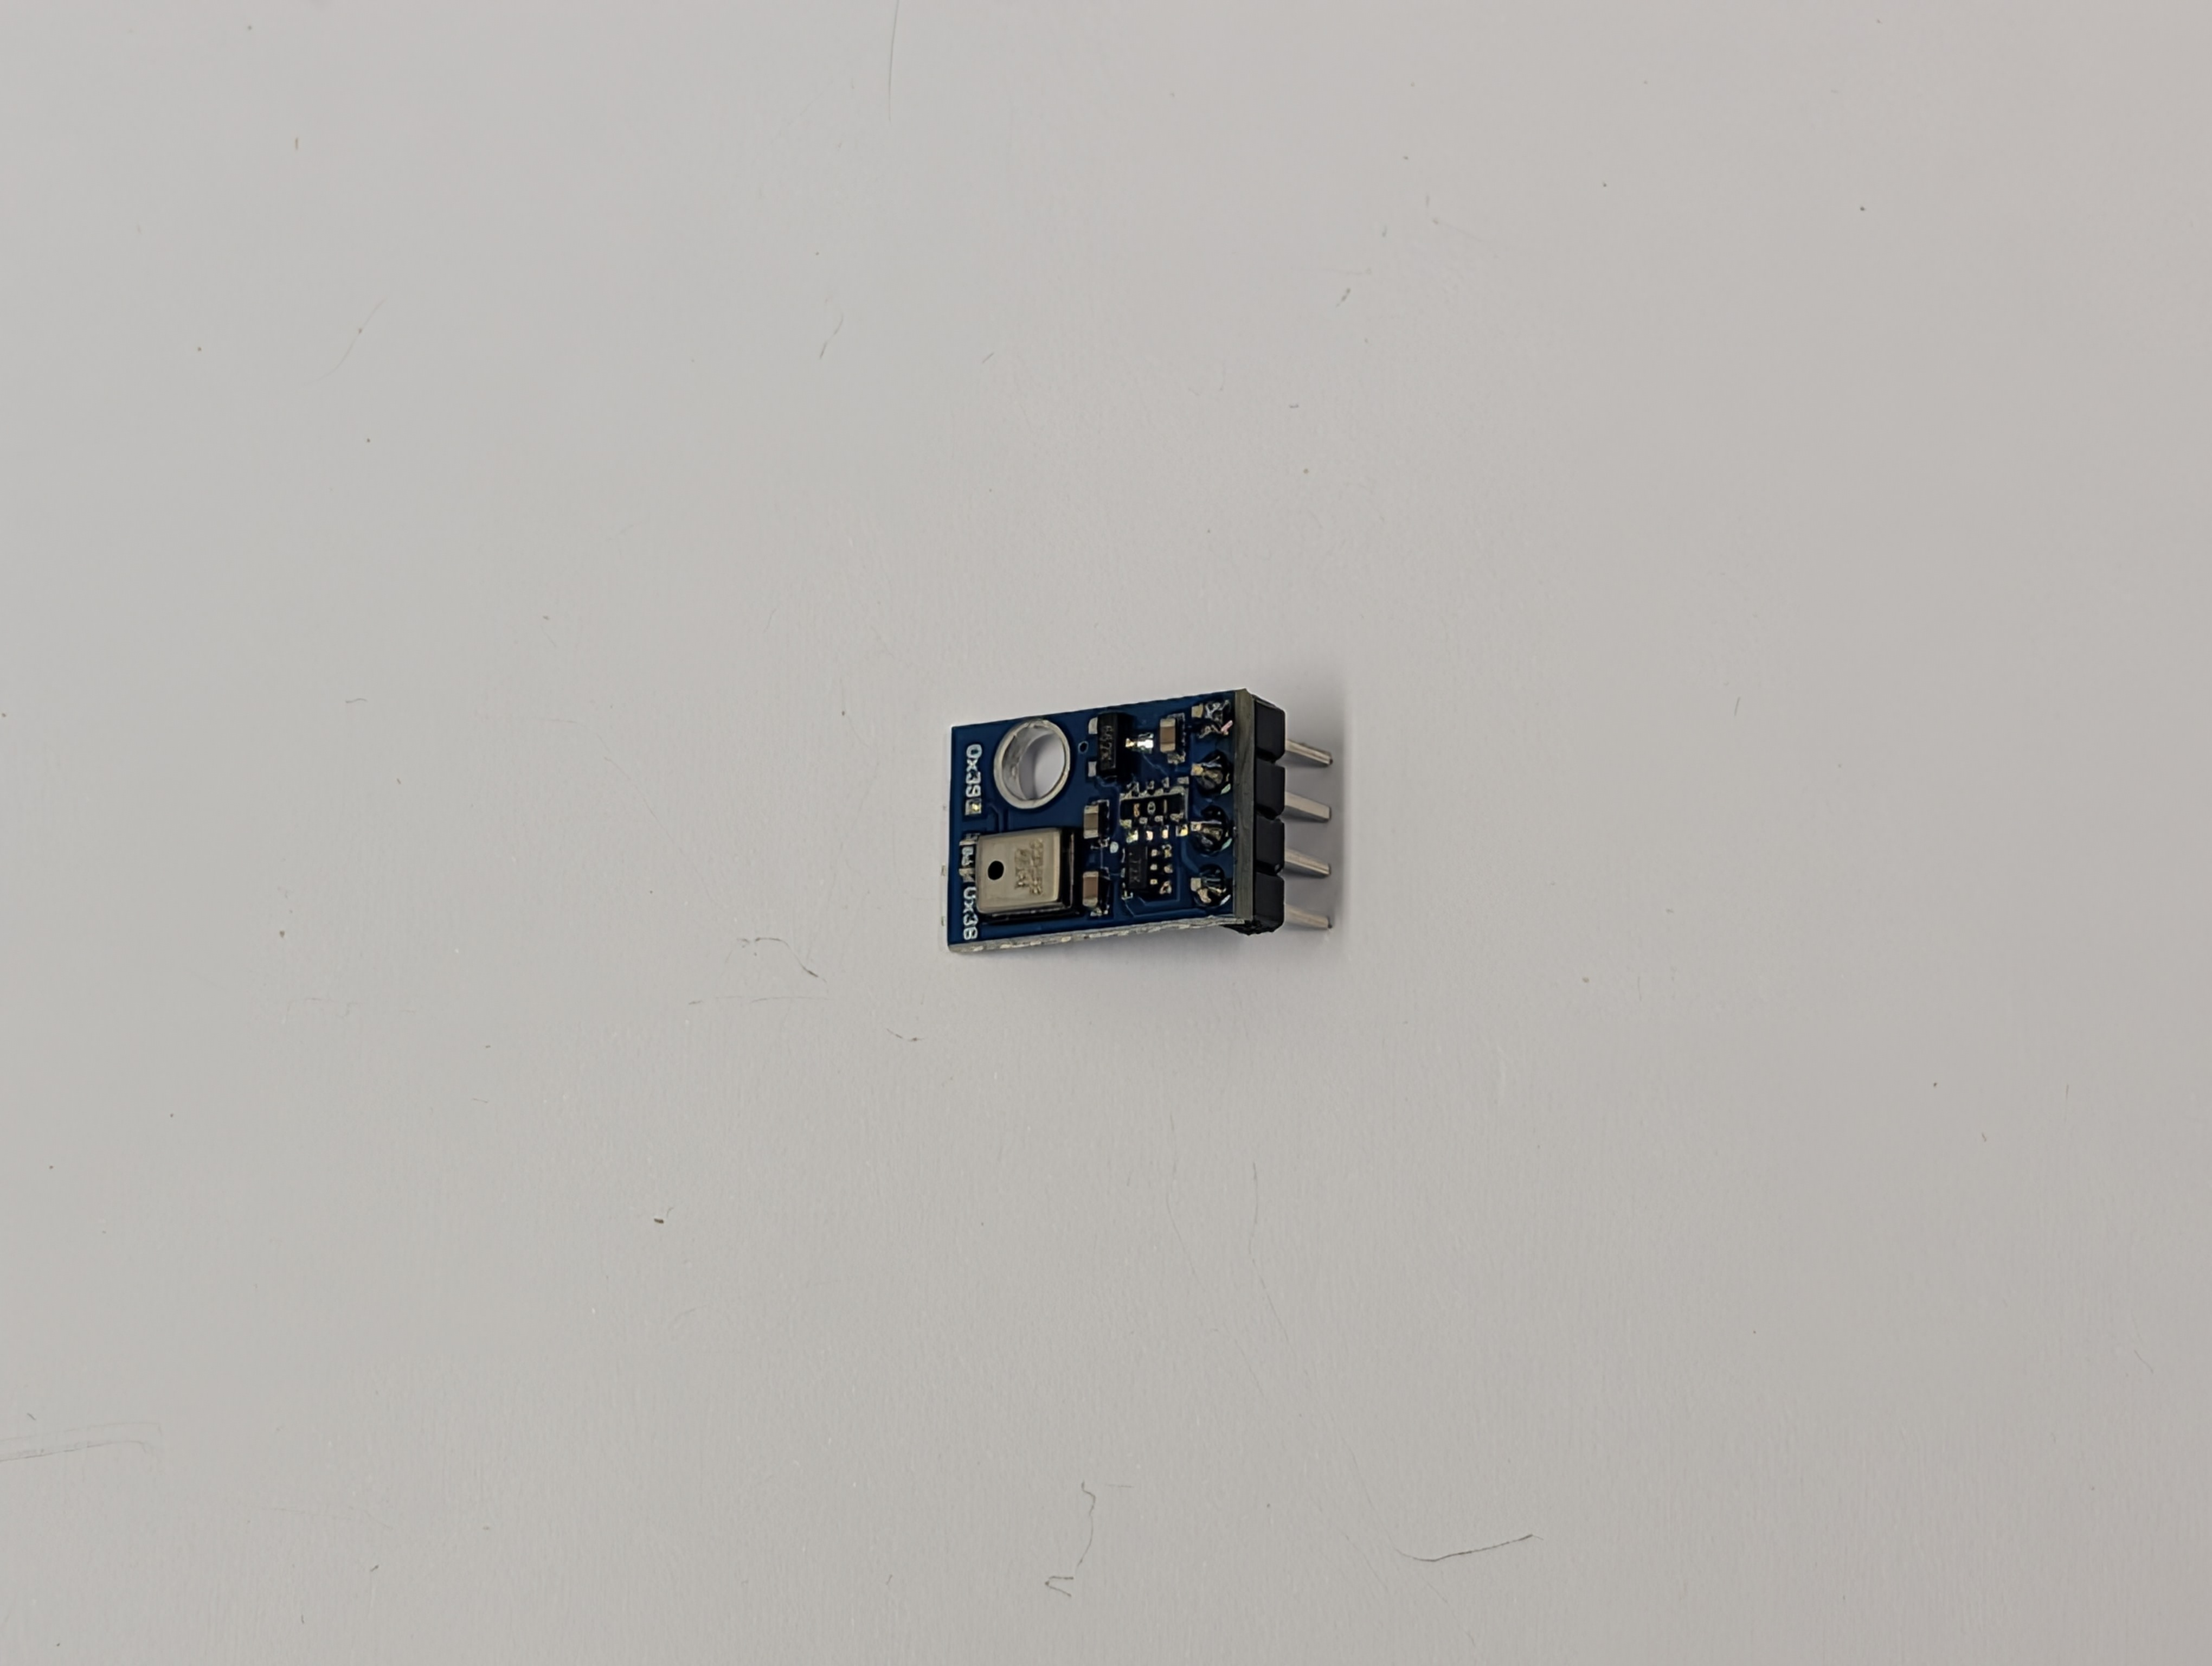
\includegraphics[width=0.75\textwidth]{pictures_of_construction/instruction_step_57.jpg}
\end{figure}

\begin{figure}[H]
    \centering
    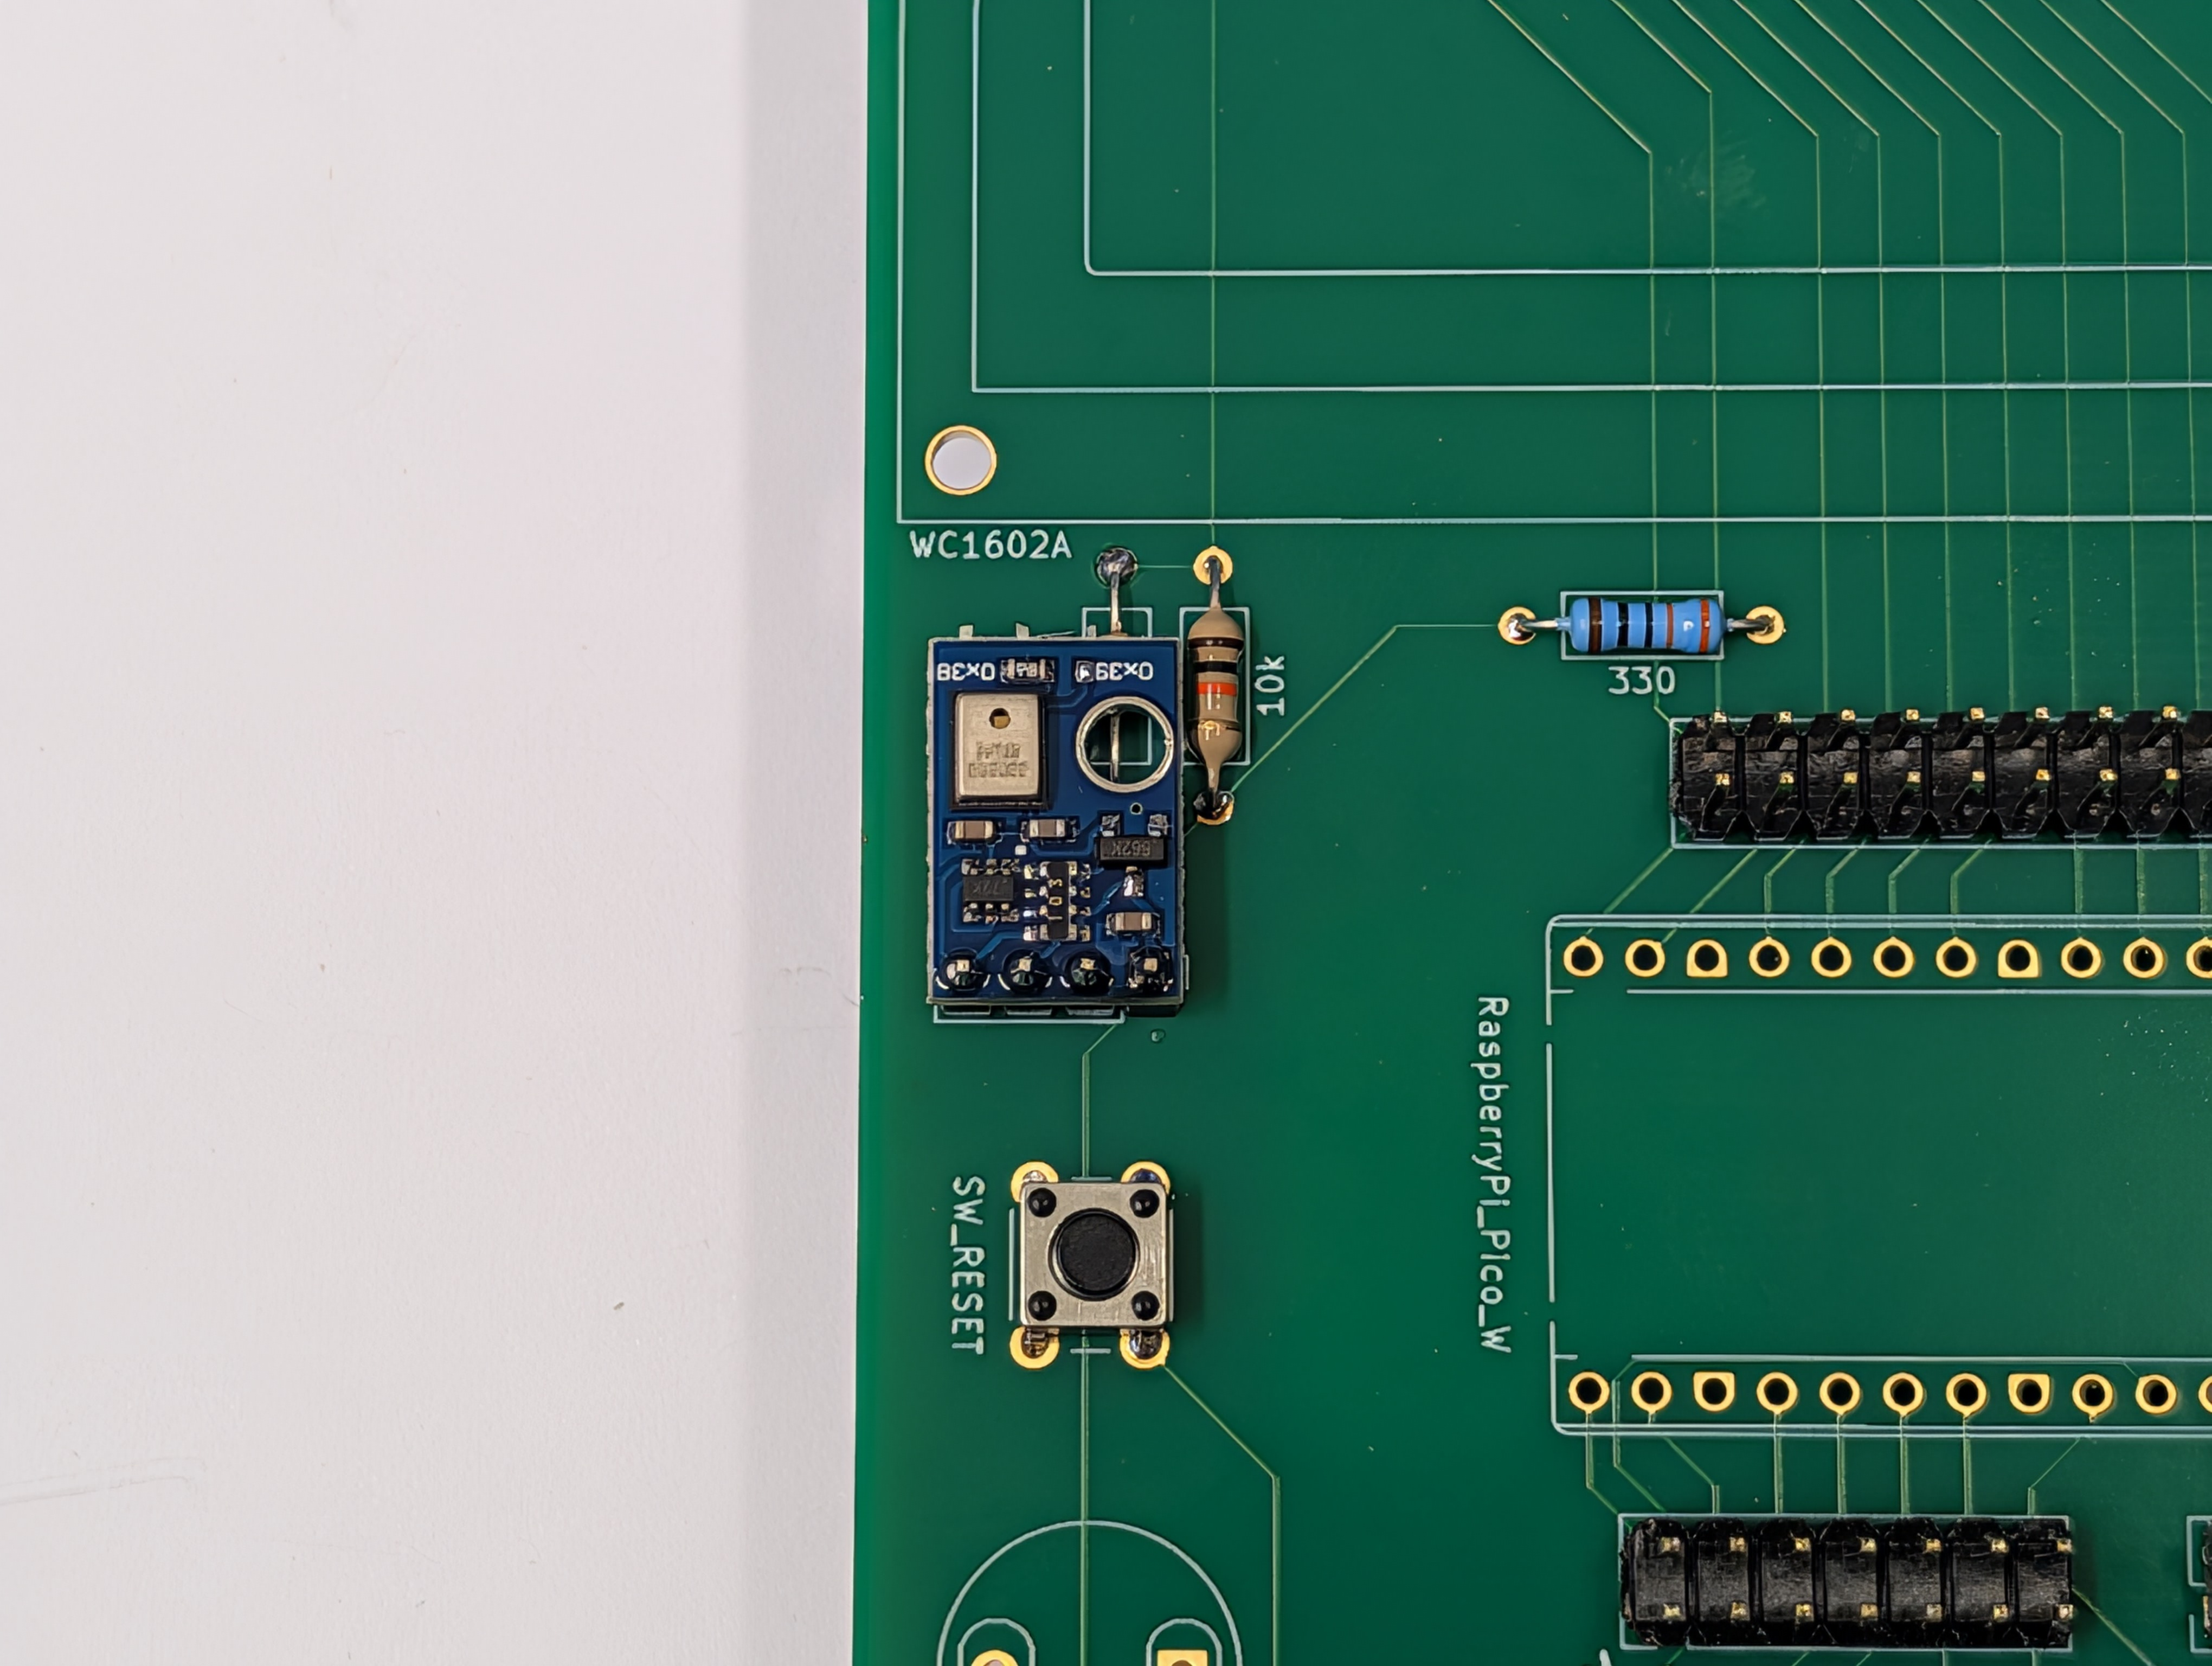
\includegraphics[width=0.75\textwidth]{pictures_of_construction/instruction_step_58.jpg}
\end{figure}

The installation of the AHT10 digital temperature sensor is analogous to the USB-C breakout board (position left side of the Buzzerino PCB, facing upwards, the components of the sub-PCB should be visible). But remember: use the larger wire cutters for cutting the pins to length.

\subsection*{Installation of the Buzzer}

\begin{figure}[H]
    \centering
    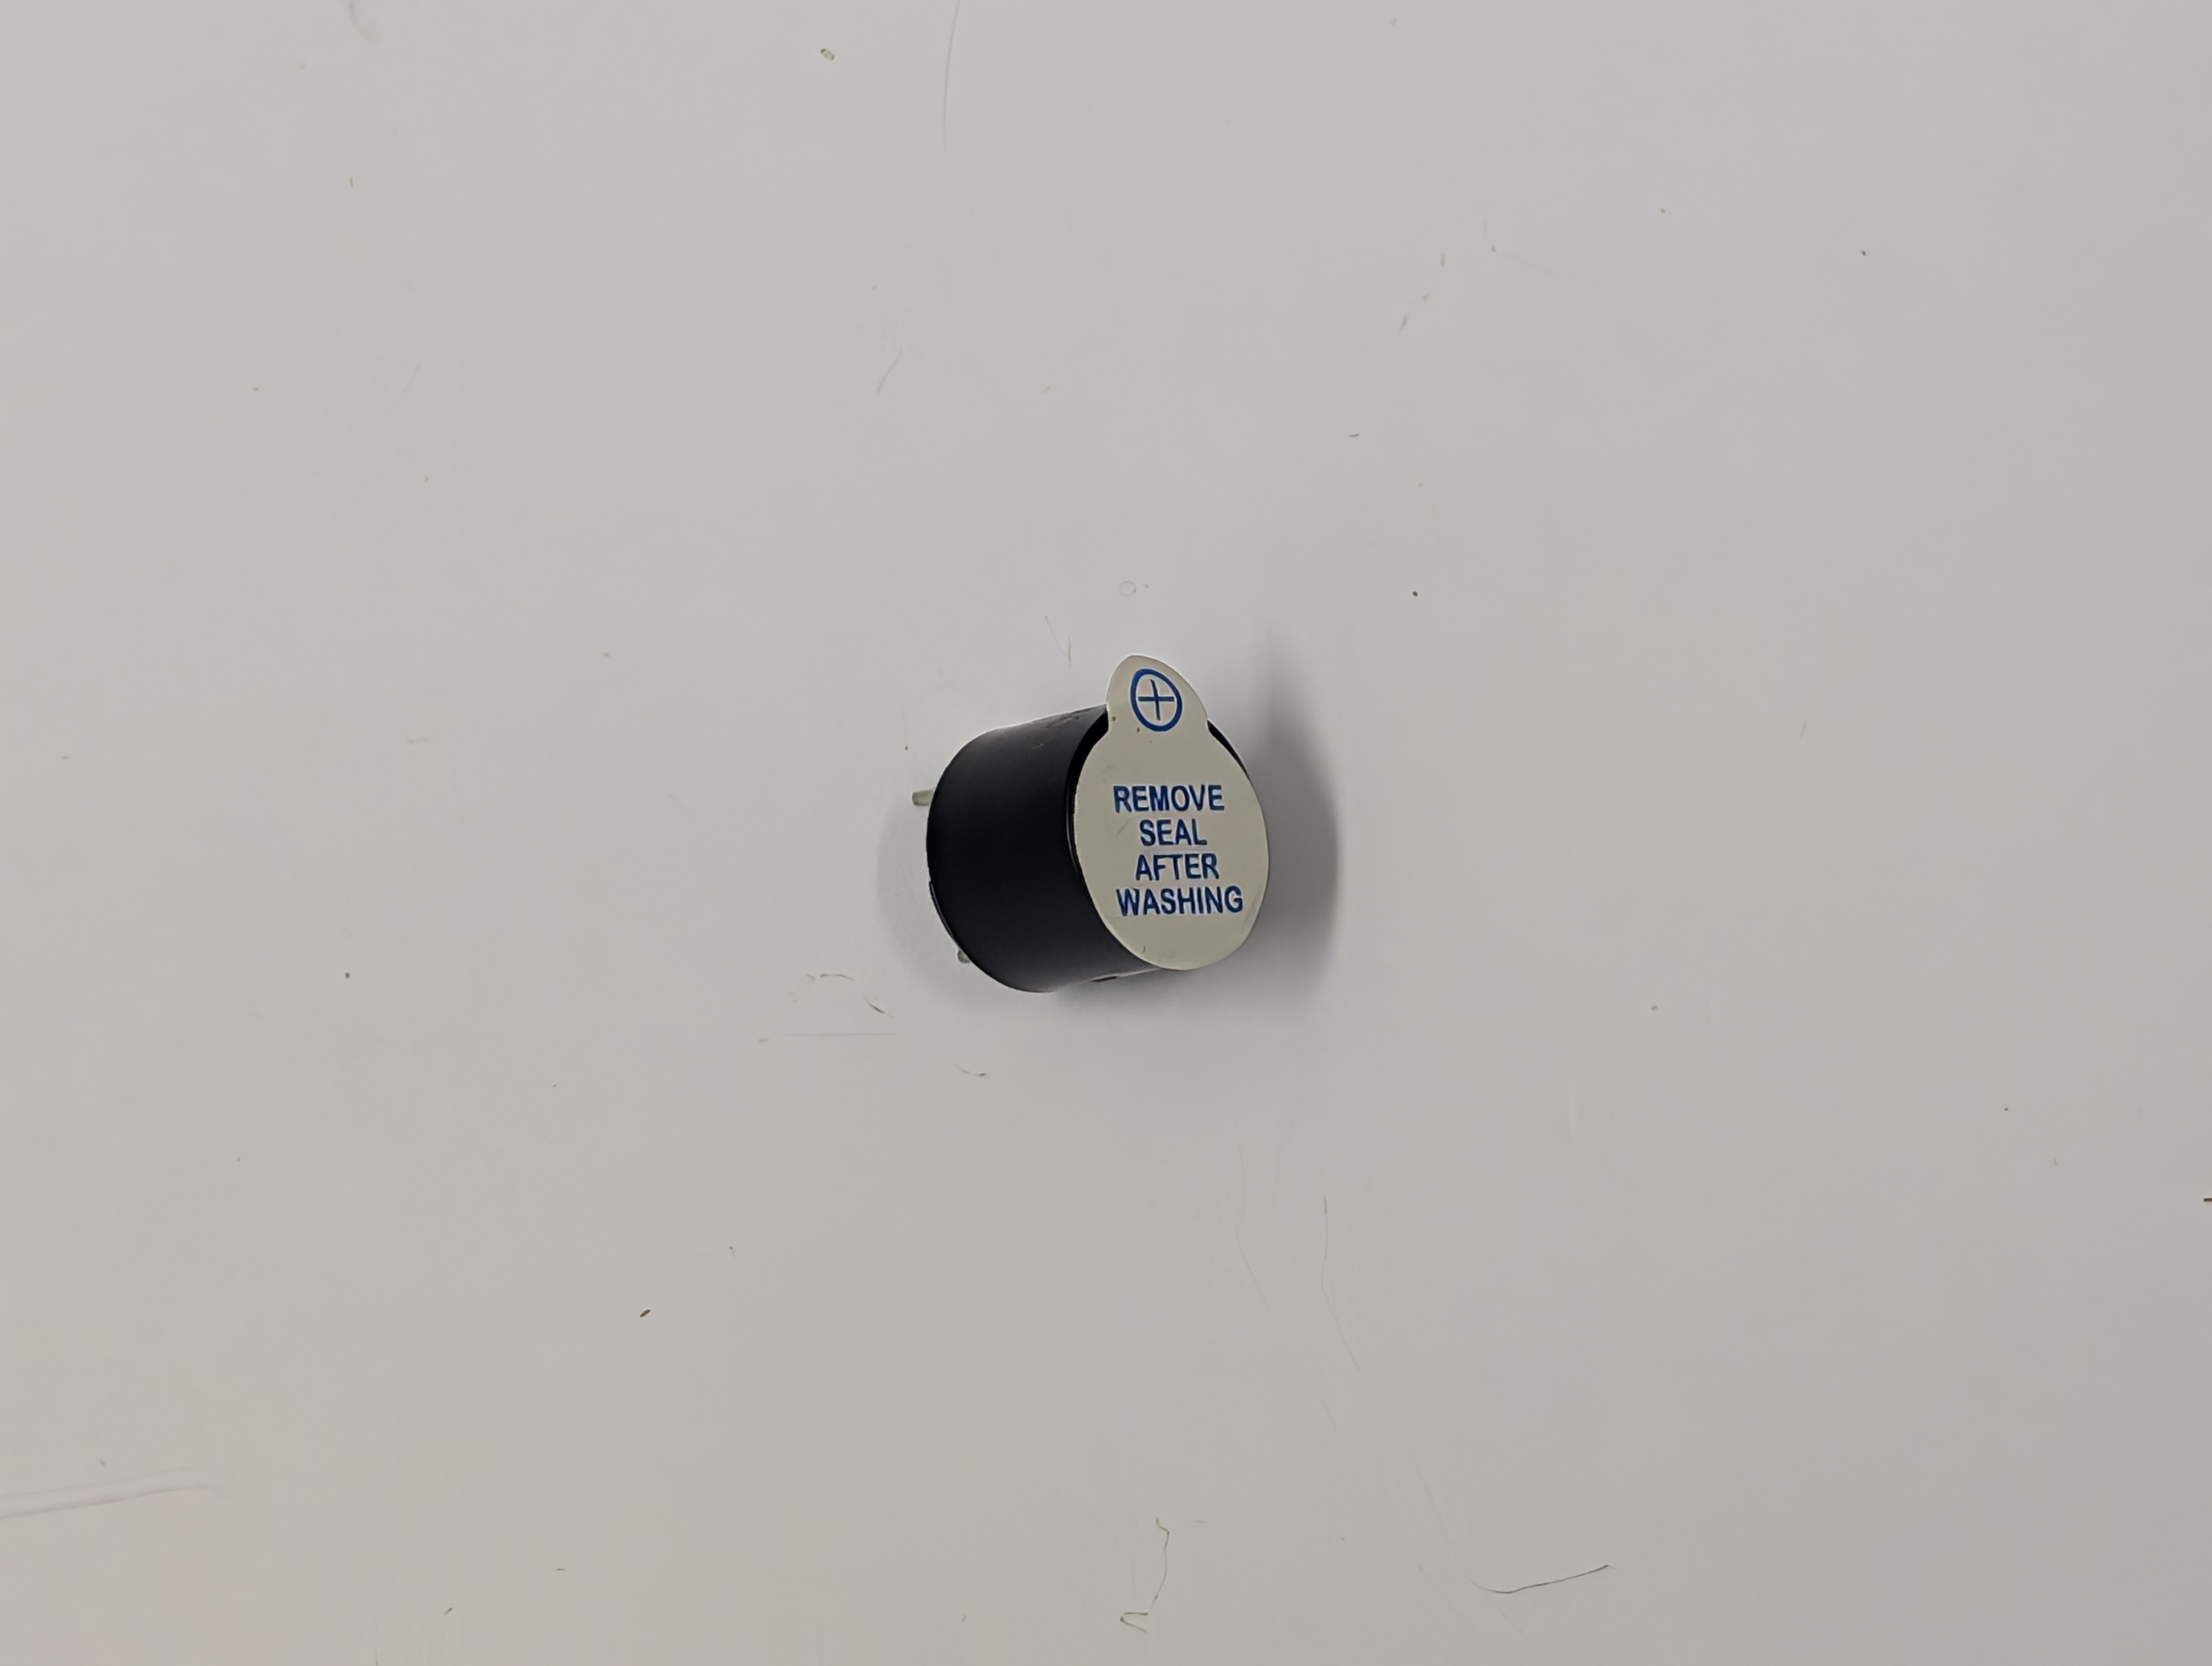
\includegraphics[width=0.75\textwidth]{pictures_of_construction/instruction_step_59.jpg}
\end{figure}

\begin{figure}[H]
    \centering
    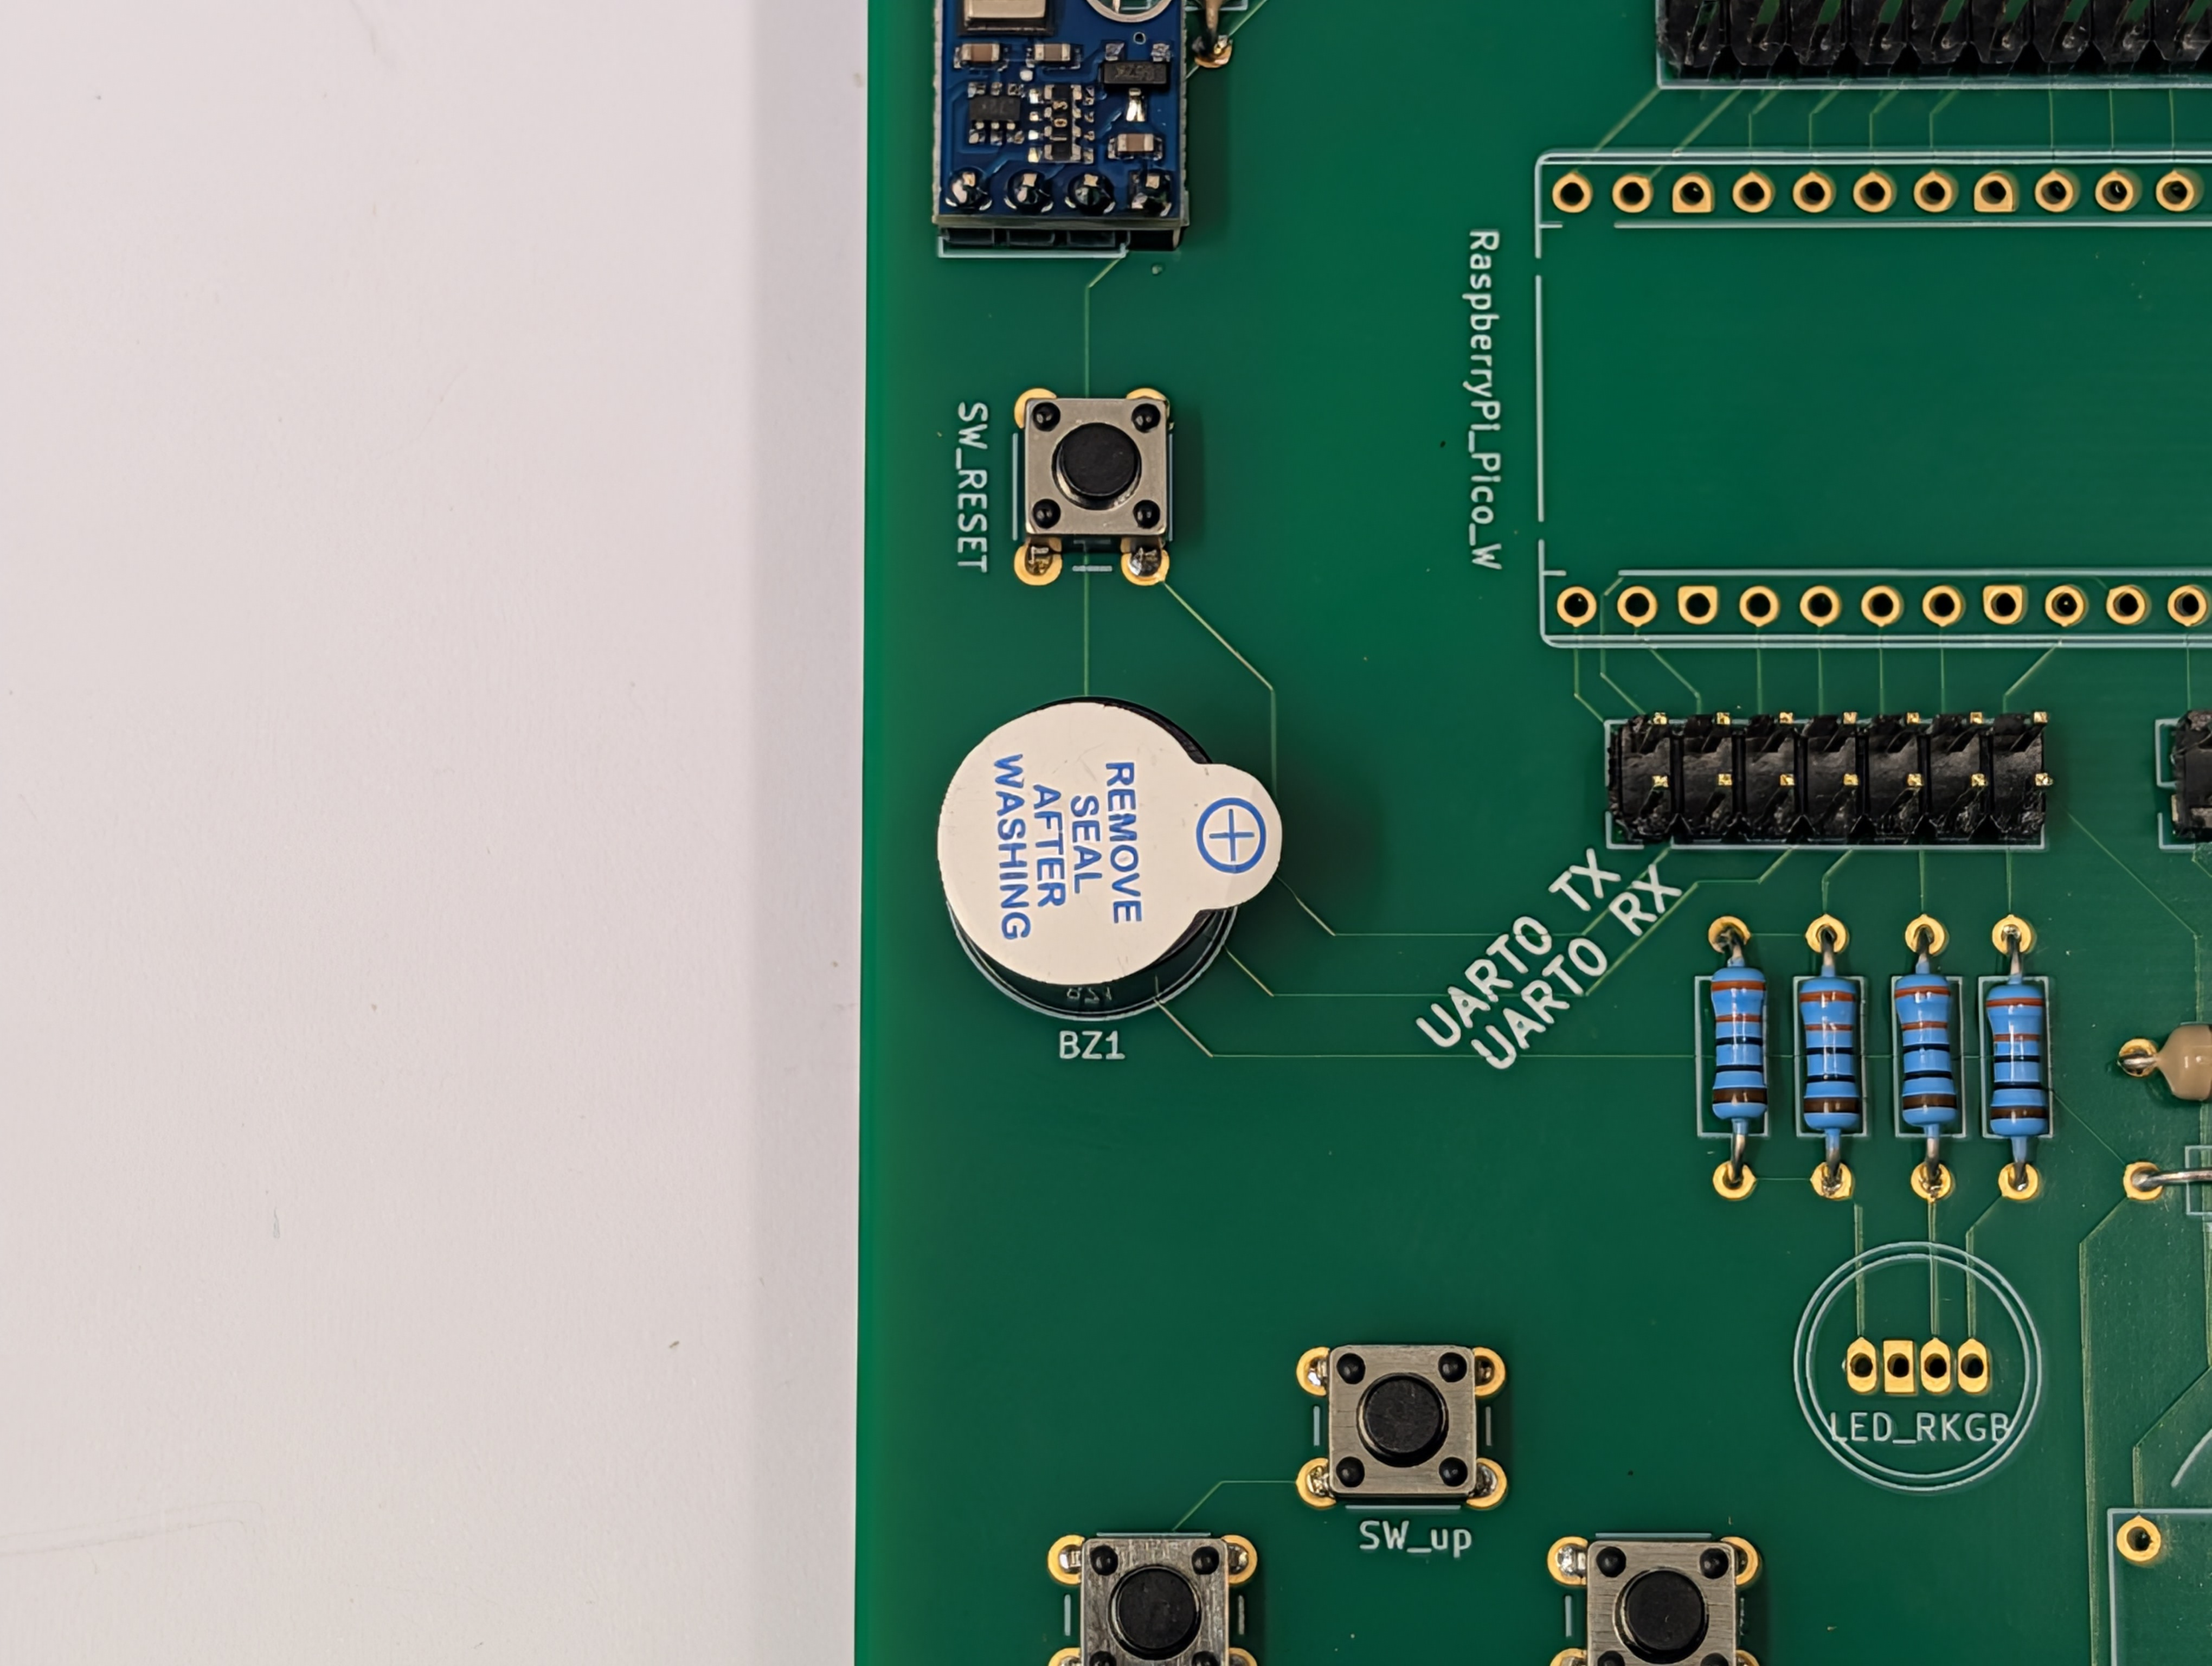
\includegraphics[width=0.75\textwidth]{pictures_of_construction/instruction_step_60.jpg}
\end{figure}

Finally, we can install the namesake of the board. This is our first polarized component. The footprint on the Buzzerino PCB shows a small \texttt{+}. Furthermore, the sticker on the buzzer has a plus on its top. These should be aligned. (If you look from the front of the Buzzerino PCB, the plus will be facing inwards.) Moreover, if you are unsure, you can check the buzzer's leads: one of them is longer than the other. This is the positive lead and shall align with the plus symbol on the Buzzerino PCB.

\subsection*{Installation of the 1602A LCD display}

\begin{figure}[H]
    \centering
    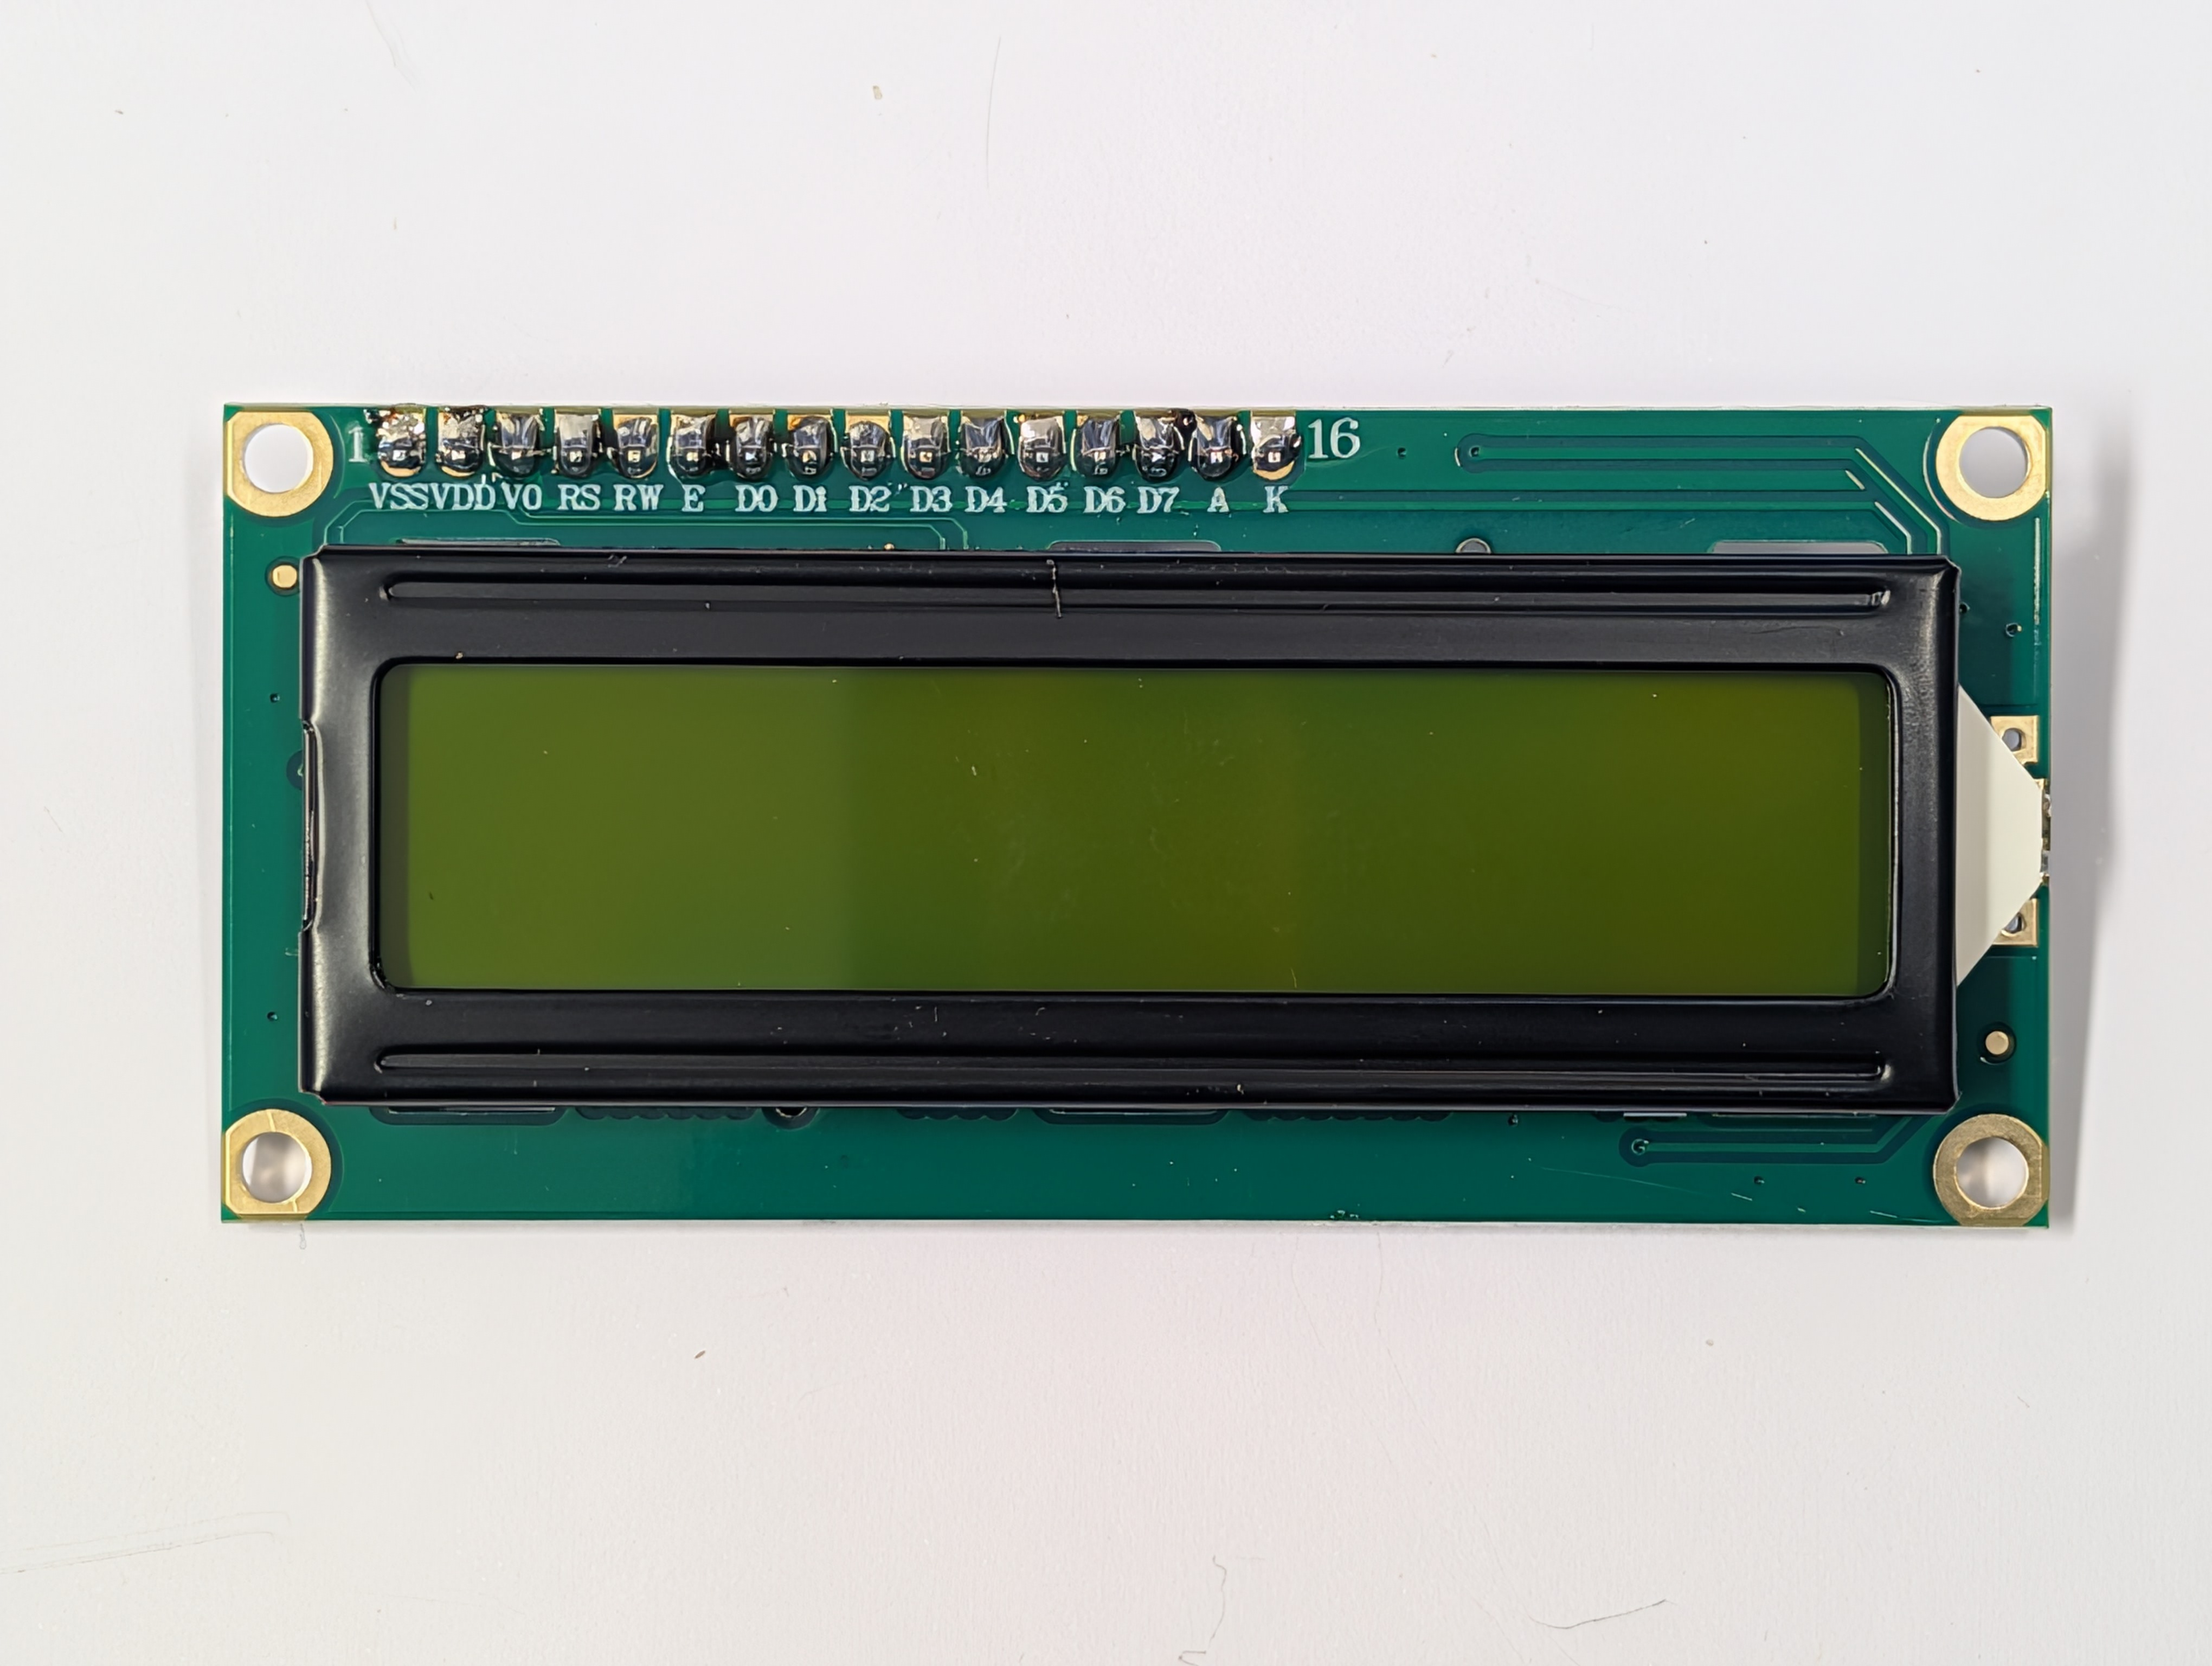
\includegraphics[width=0.75\textwidth]{pictures_of_construction/instruction_step_61.jpg}
\end{figure}

\begin{figure}[H]
    \centering
    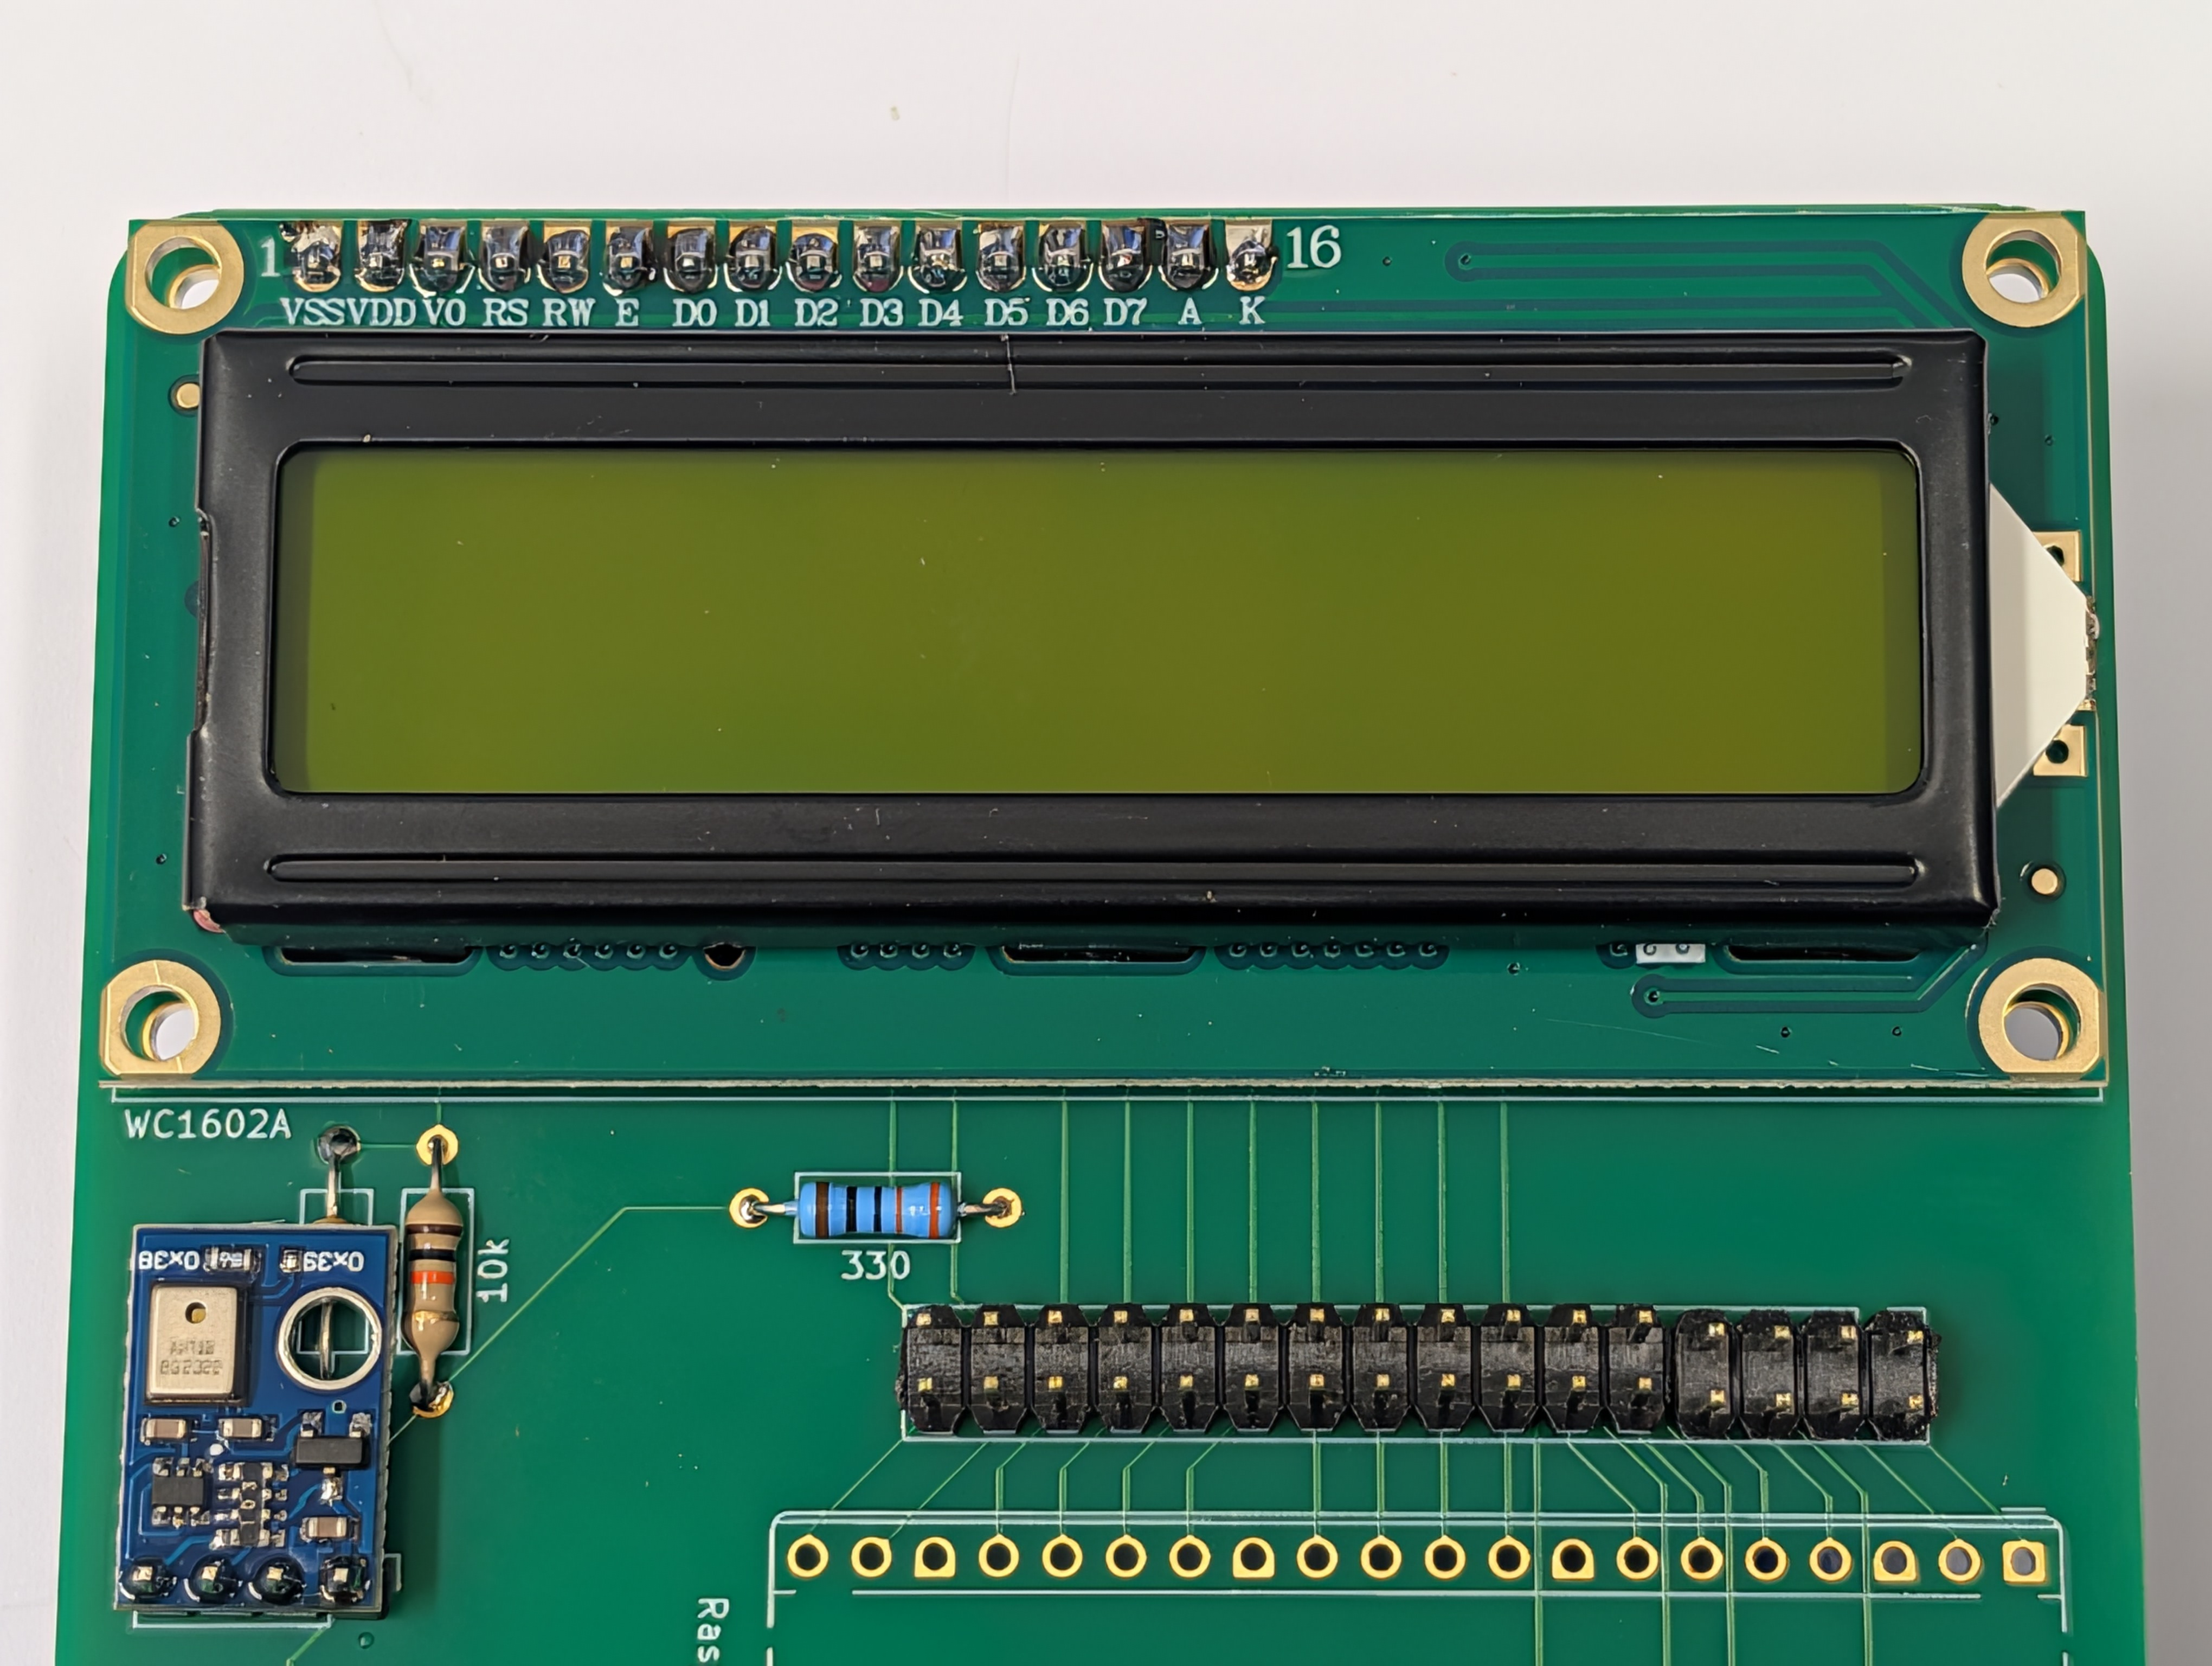
\includegraphics[width=0.75\textwidth]{pictures_of_construction/instruction_step_62.jpg}
\end{figure}

\begin{figure}[H]
    \centering
    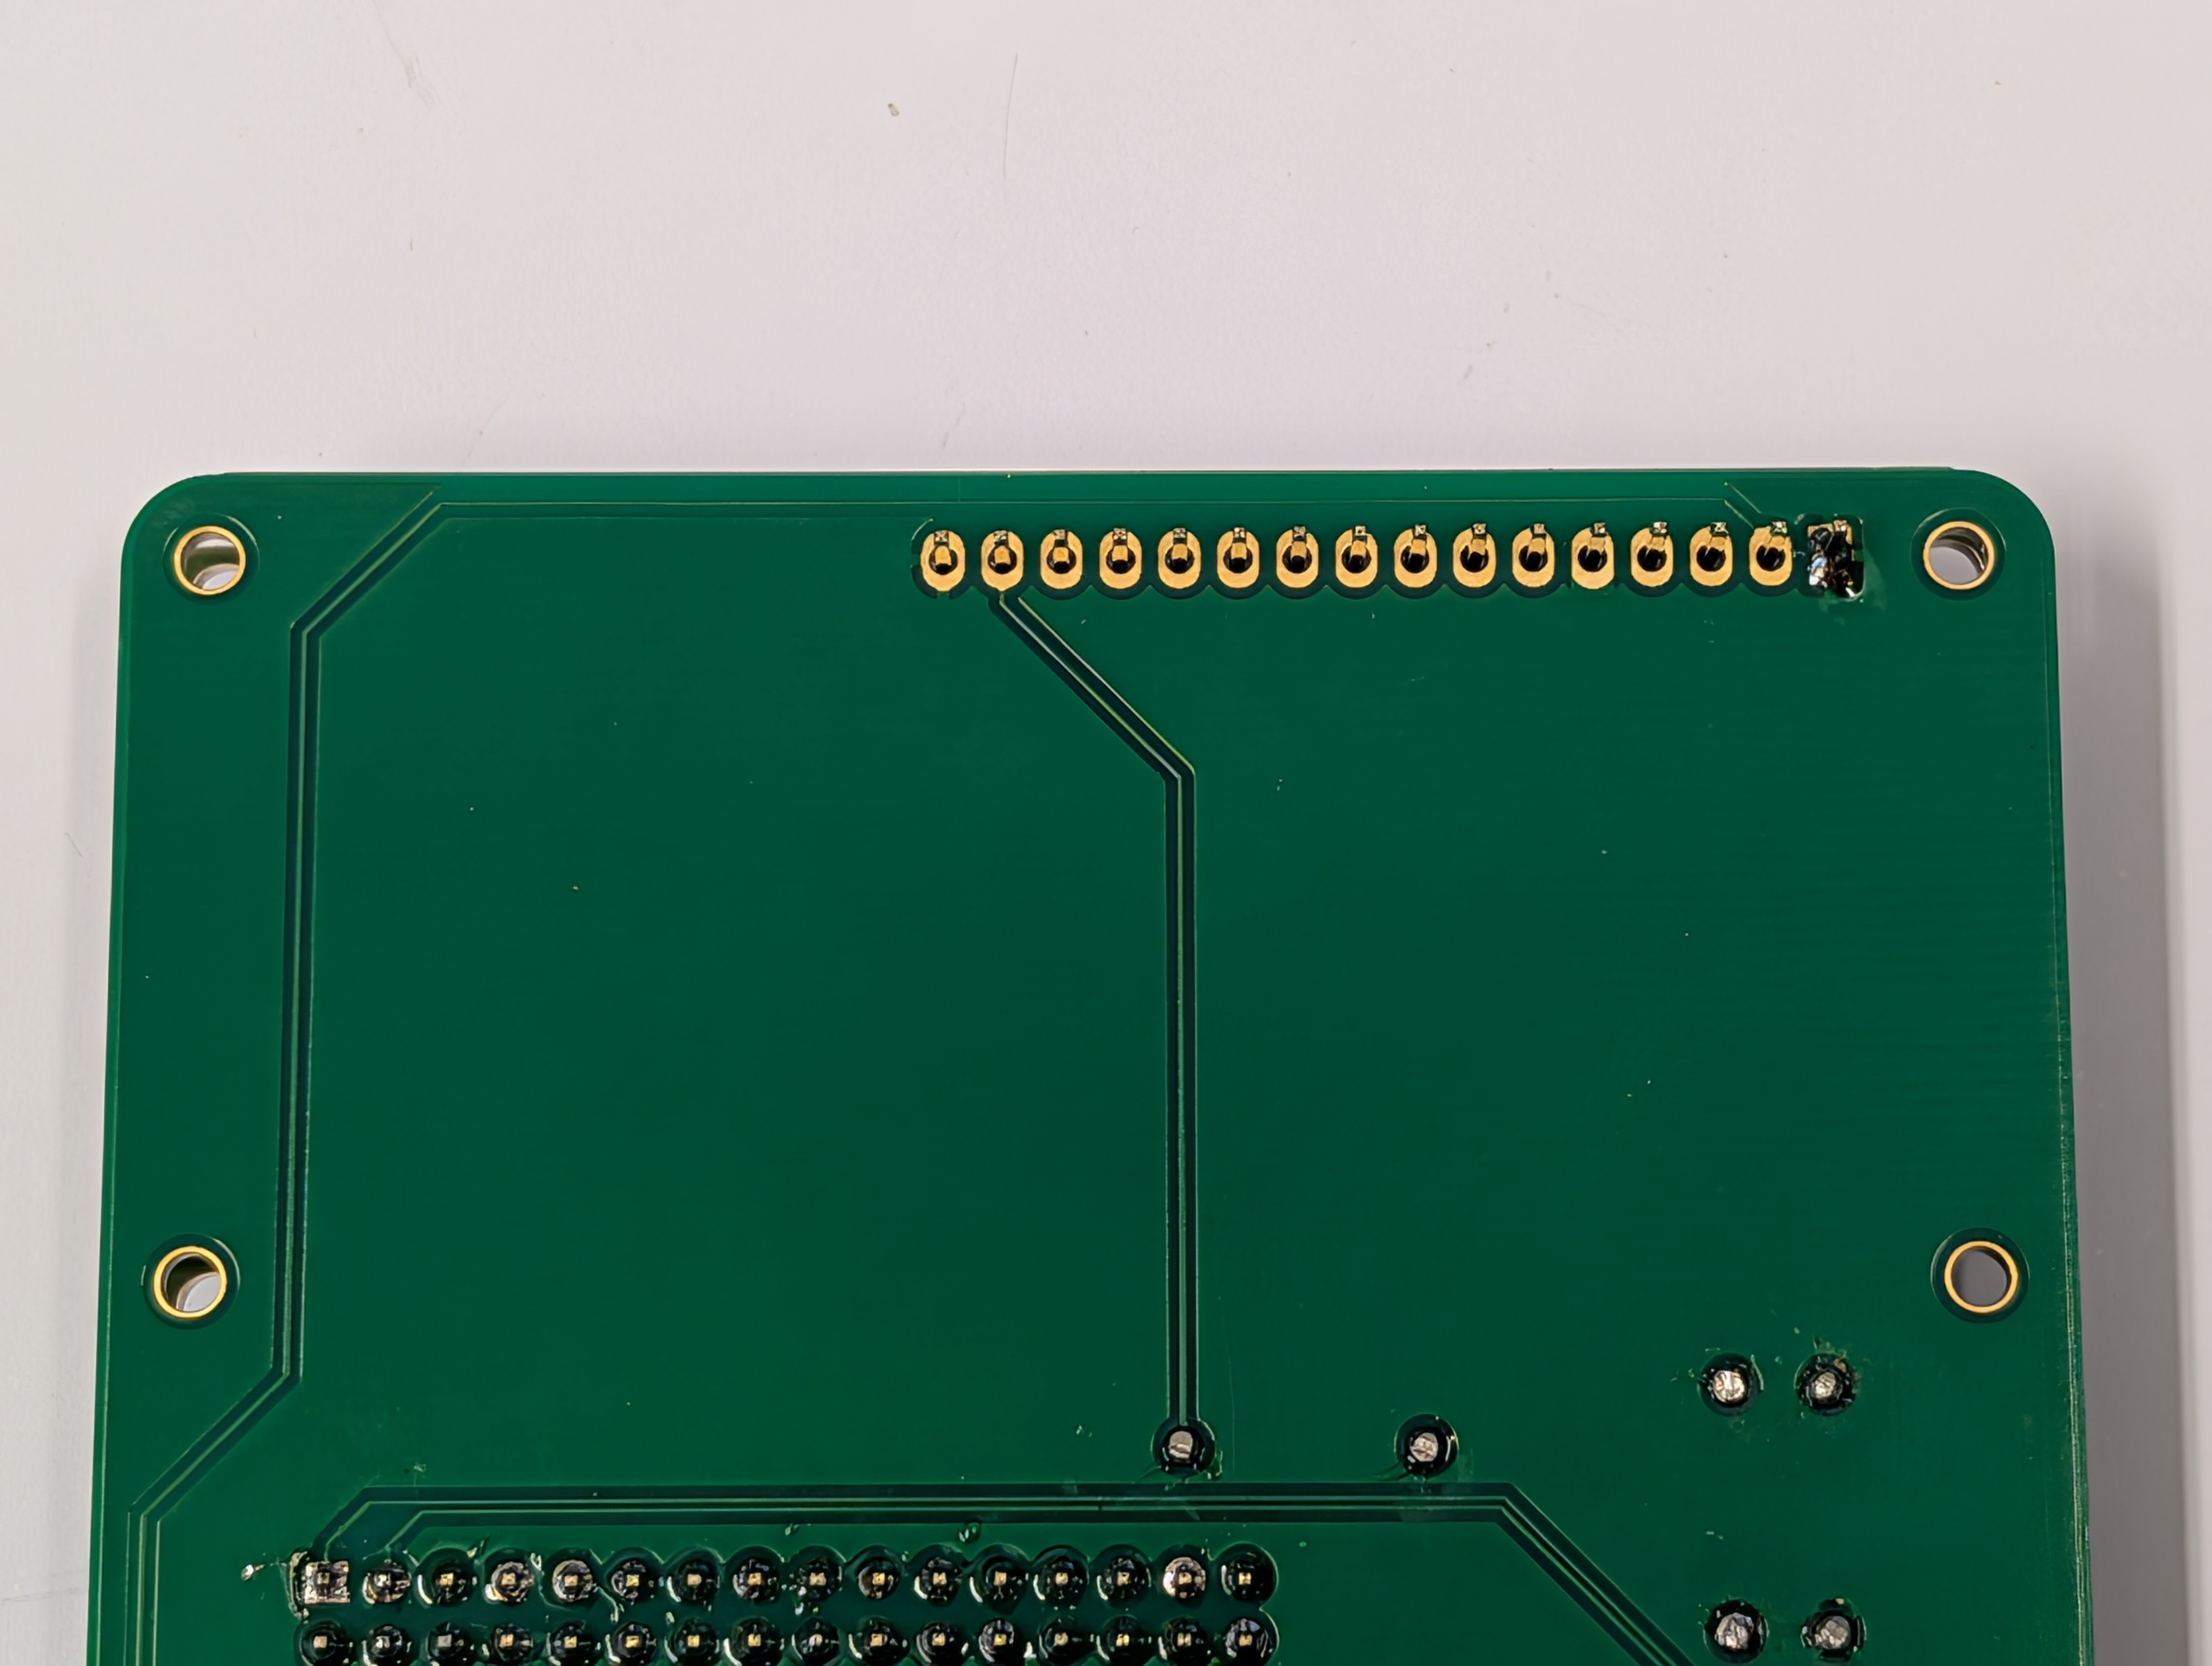
\includegraphics[width=0.75\textwidth]{pictures_of_construction/instruction_step_63.jpg}
\end{figure}

\begin{figure}[H]
    \centering
    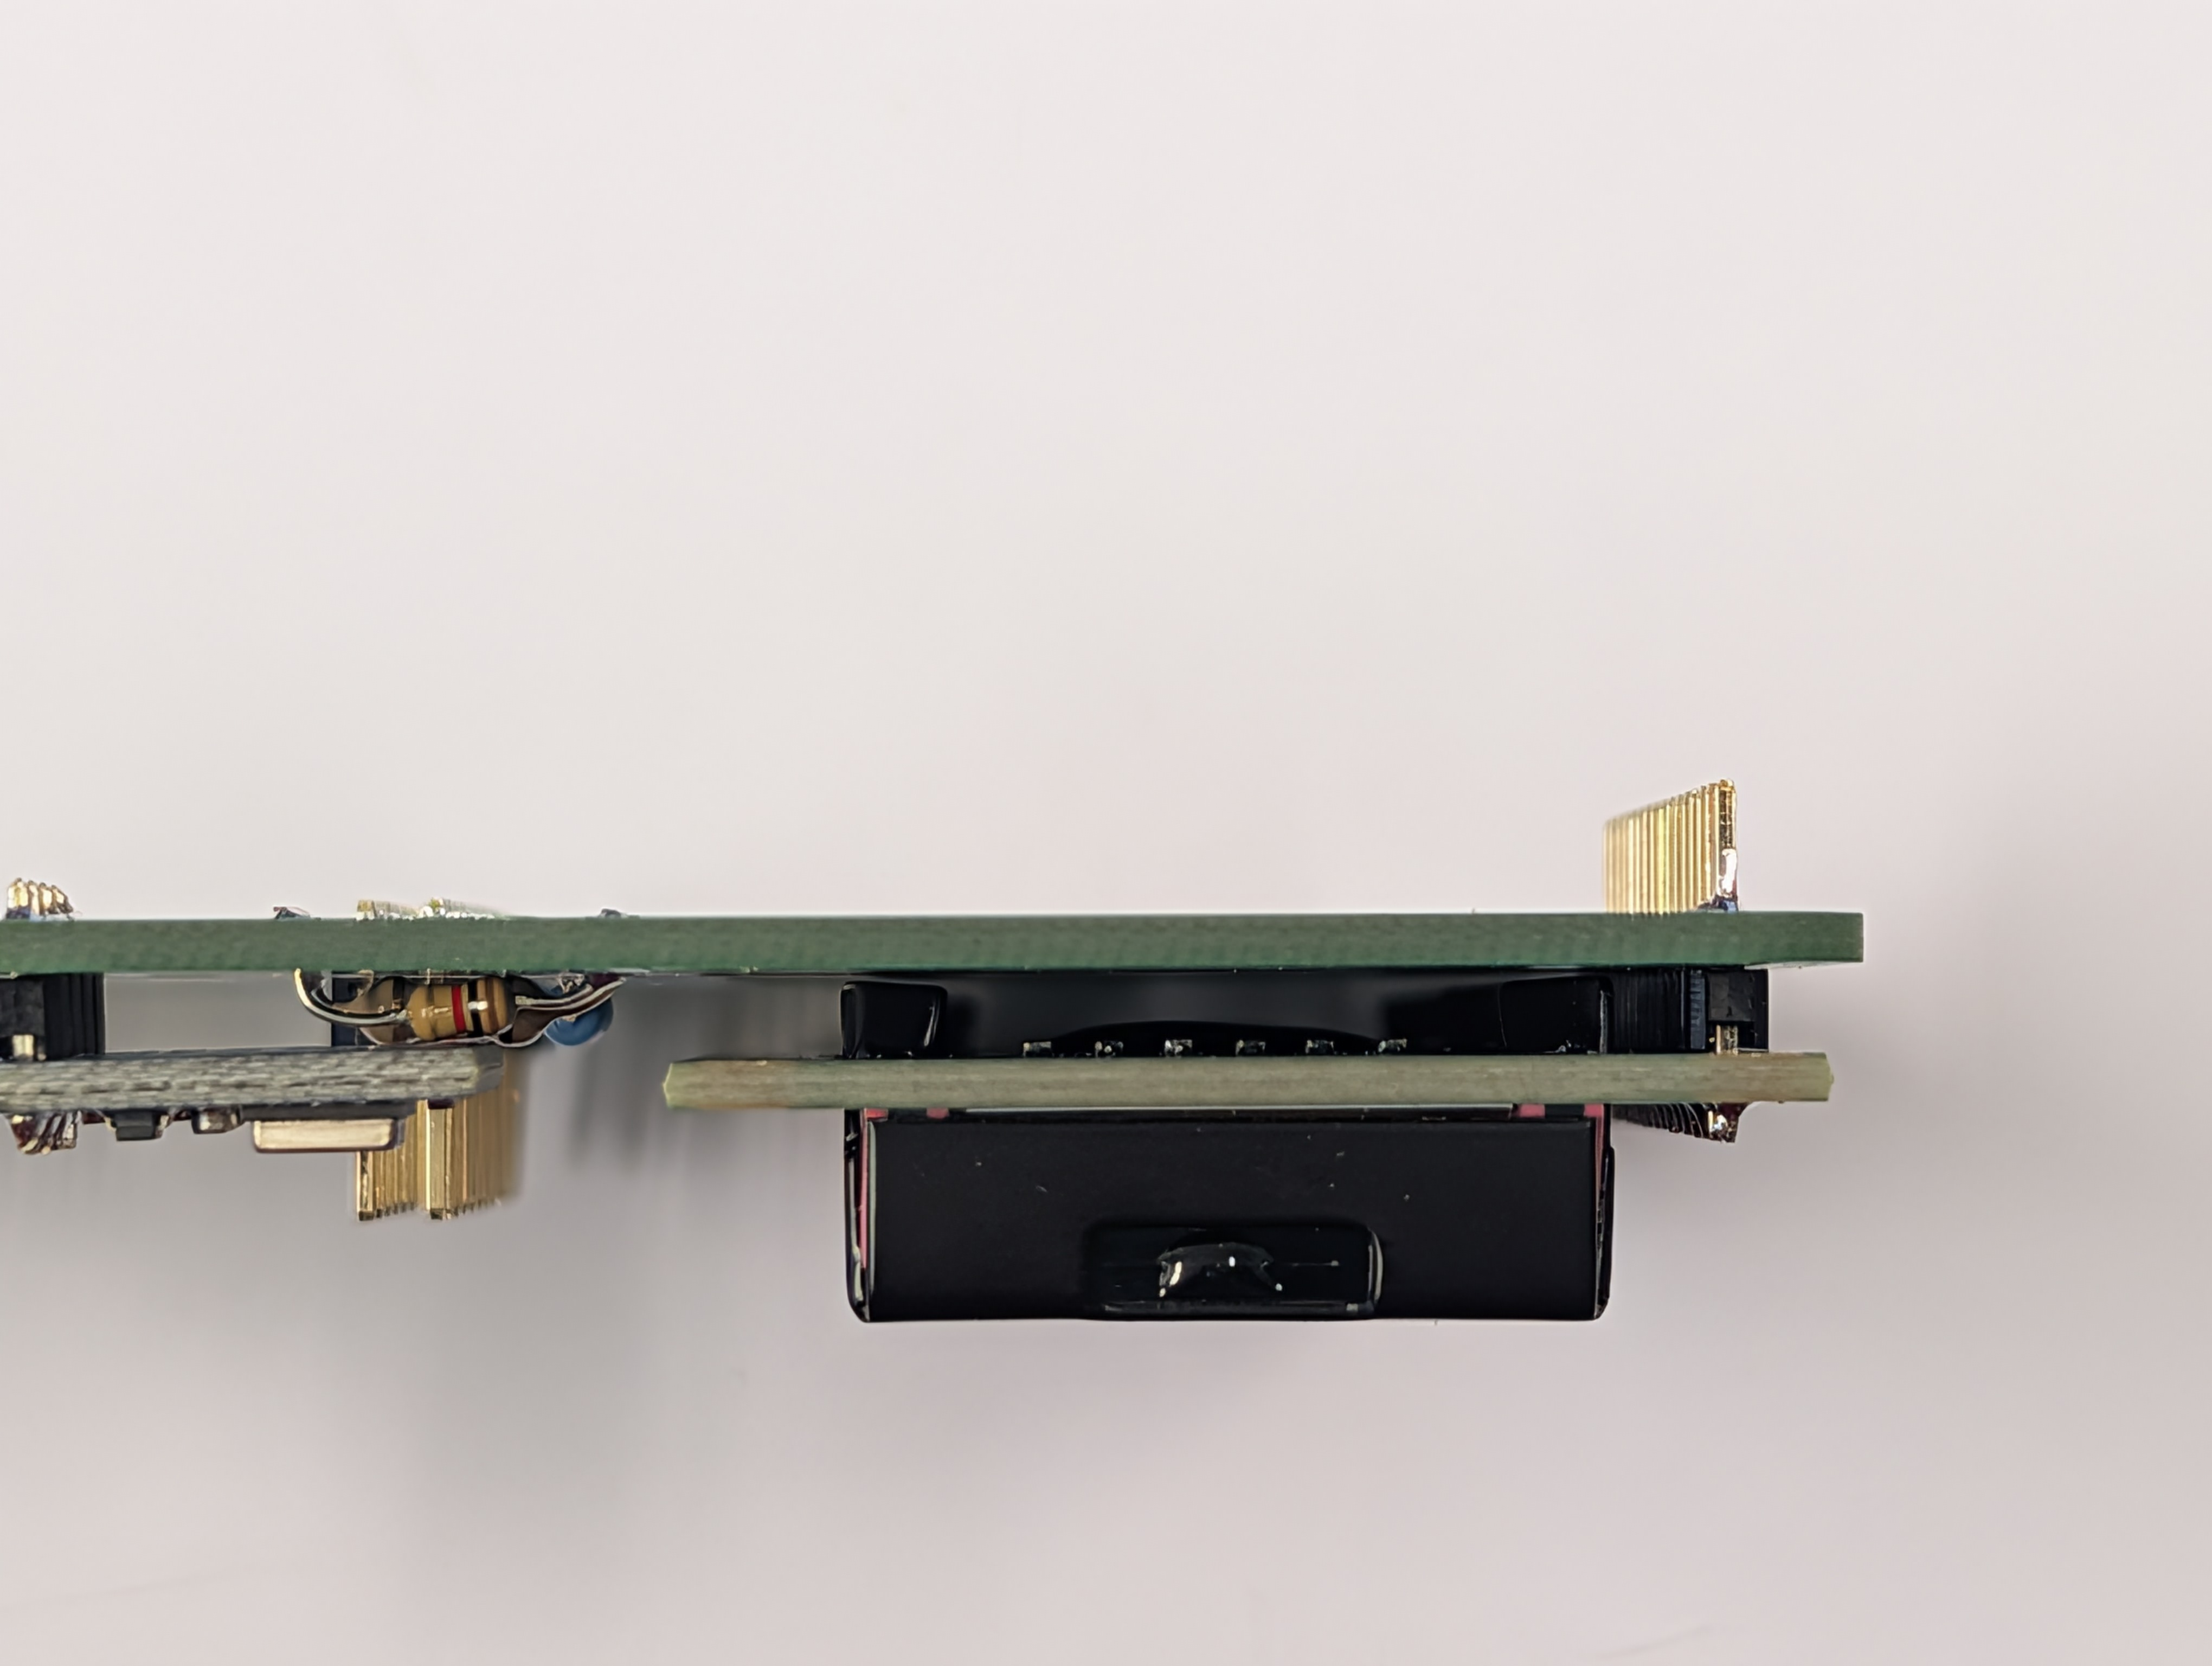
\includegraphics[width=0.75\textwidth]{pictures_of_construction/instruction_step_64.jpg}
\end{figure}

The installation of the 1602A LCD display is analogous to the USB-C breakout board. First place, then solder one pin, then check for alignment and then solder fully. But remember: use the larger wire cutters for cutting the pins to length.

\subsection*{Installation of the RGB LED}

\begin{figure}[H]
    \centering
    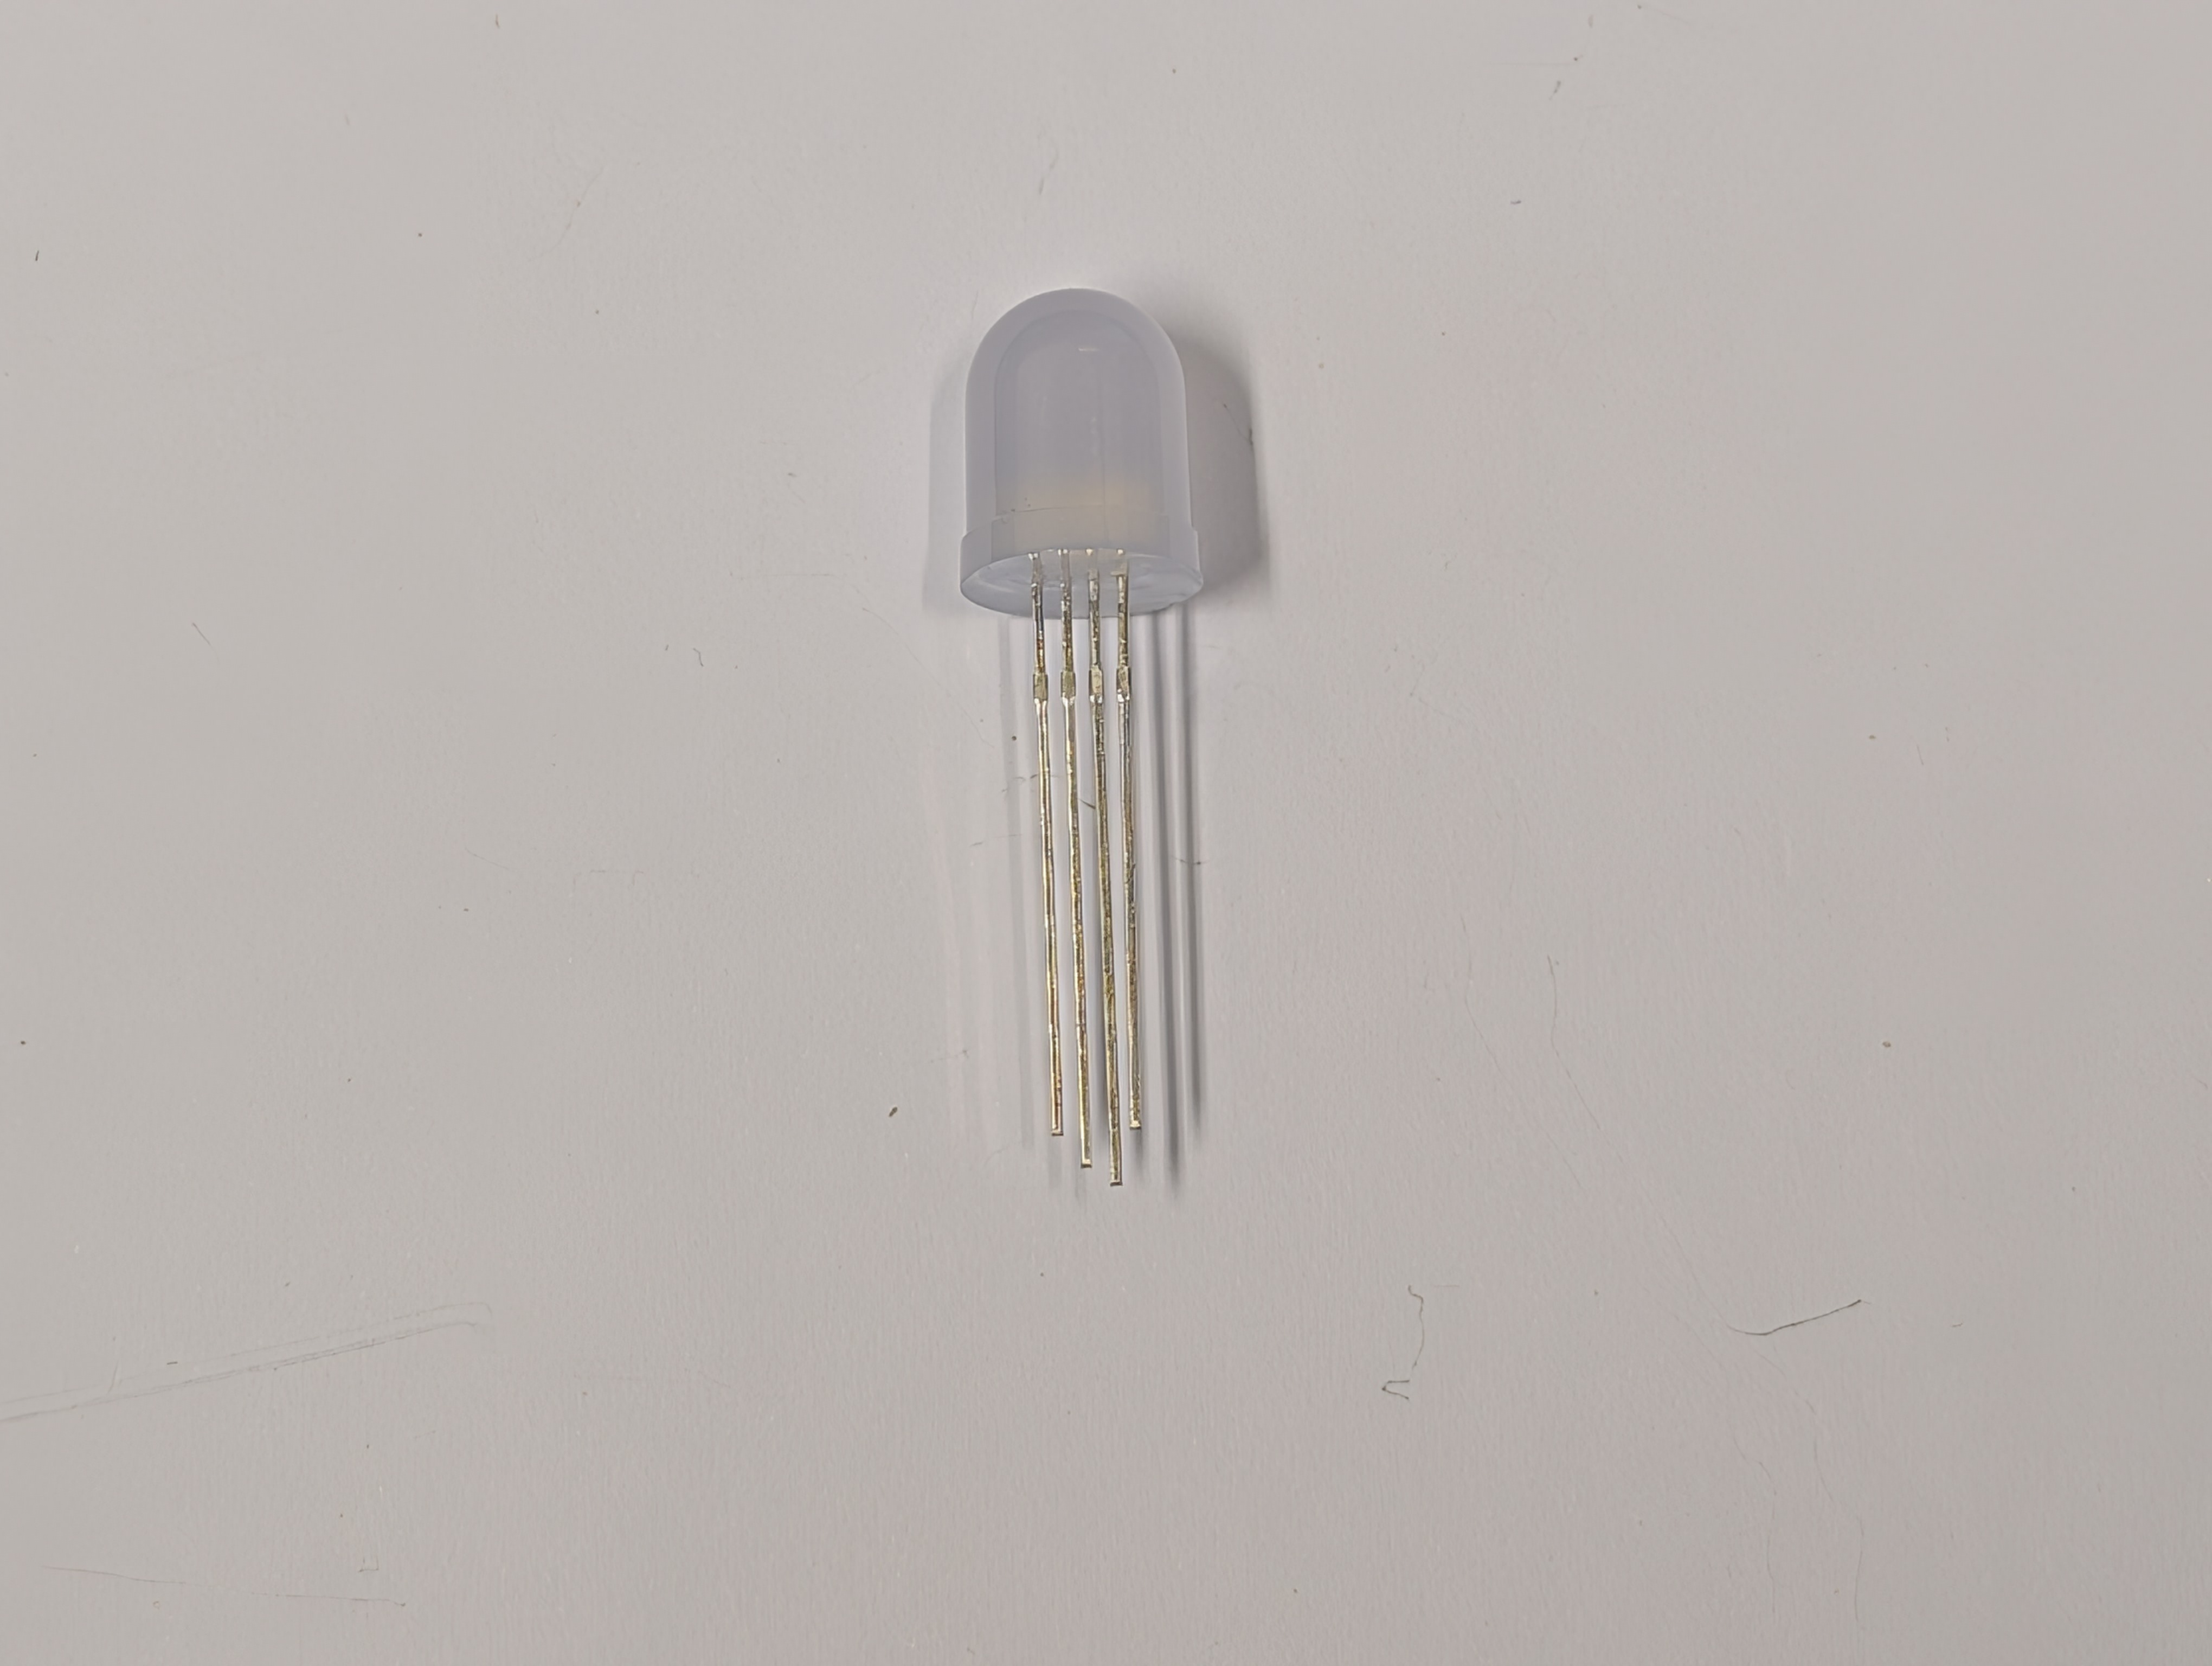
\includegraphics[width=0.75\textwidth]{pictures_of_construction/instruction_step_65.jpg}
\end{figure}

Now we can install the RGB LED.

\begin{figure}[H]
    \centering
    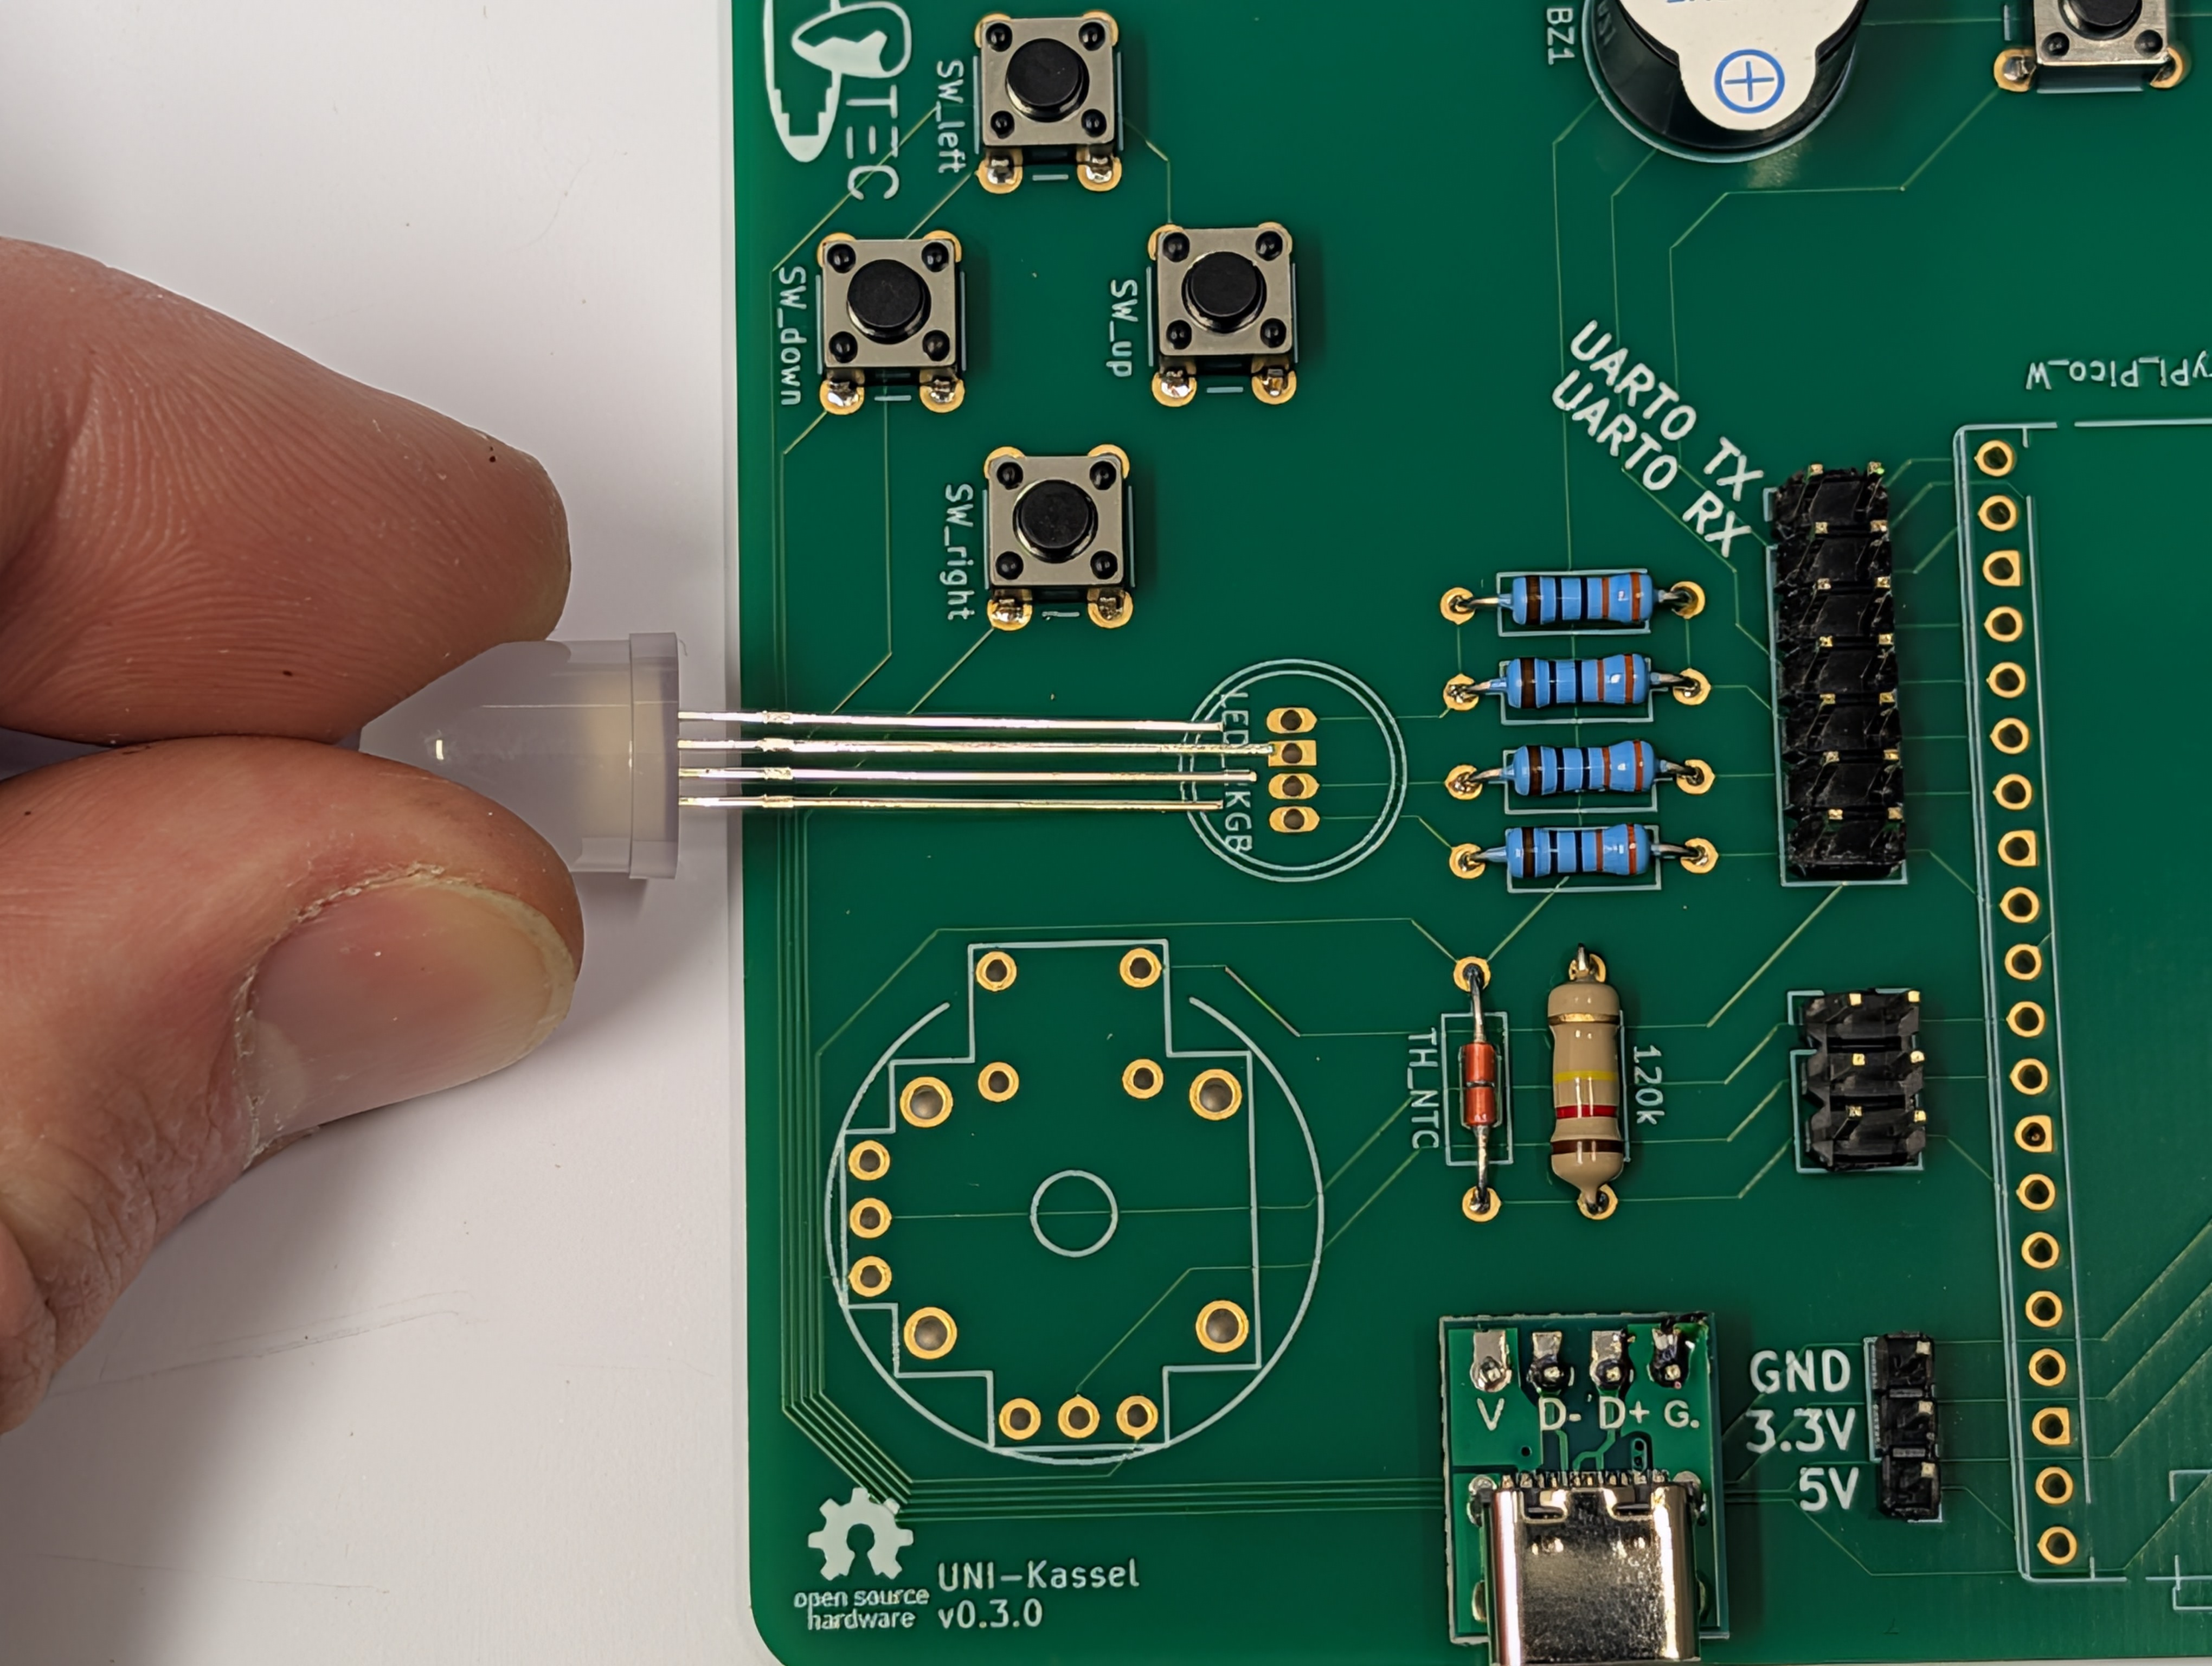
\includegraphics[width=0.75\textwidth]{pictures_of_construction/instruction_step_66.jpg}
\end{figure}

\begin{figure}[H]
    \centering
    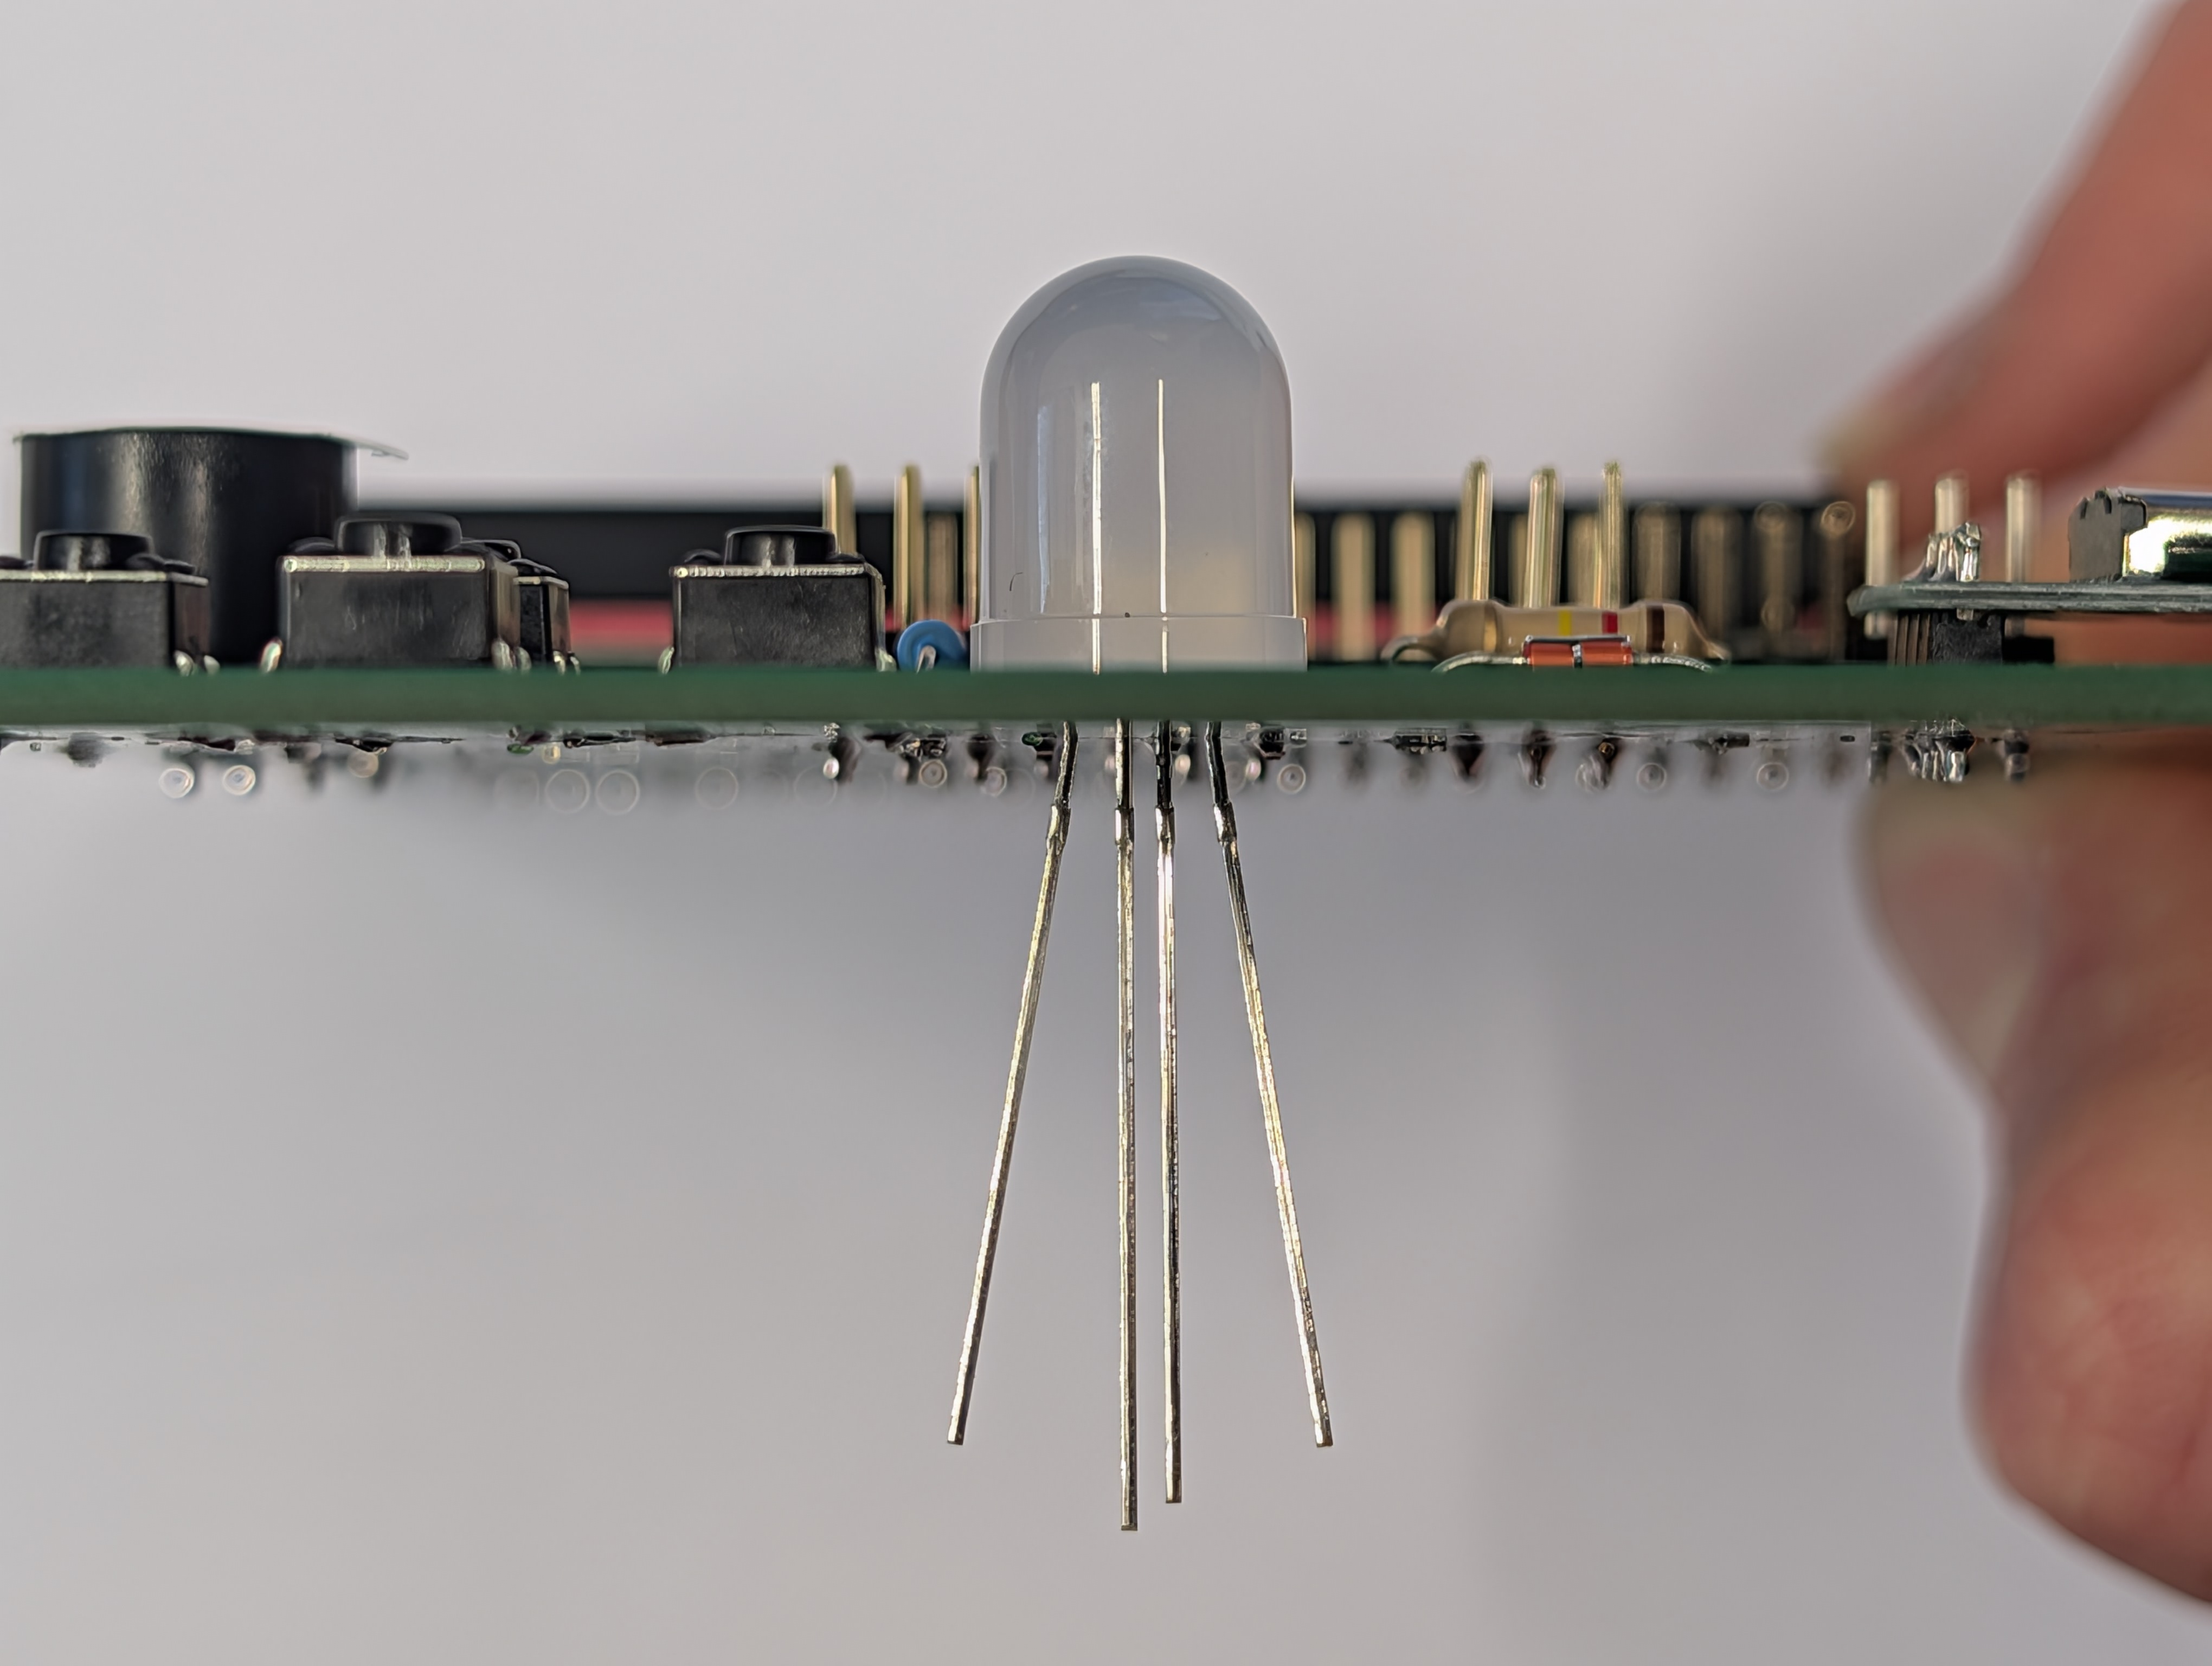
\includegraphics[width=0.75\textwidth]{pictures_of_construction/instruction_step_67.jpg}
\end{figure}

The LED is, like the buzzer, polarized. But here the longest leg is the negative connection. The footprint on the Buzzerino PCB indicates the negative connection with a square pad. Place the LED into its position. The spacing of the pads is a bit wider than the lead spacing, so the leads will spread out automatically.

\begin{figure}[H]
    \centering
    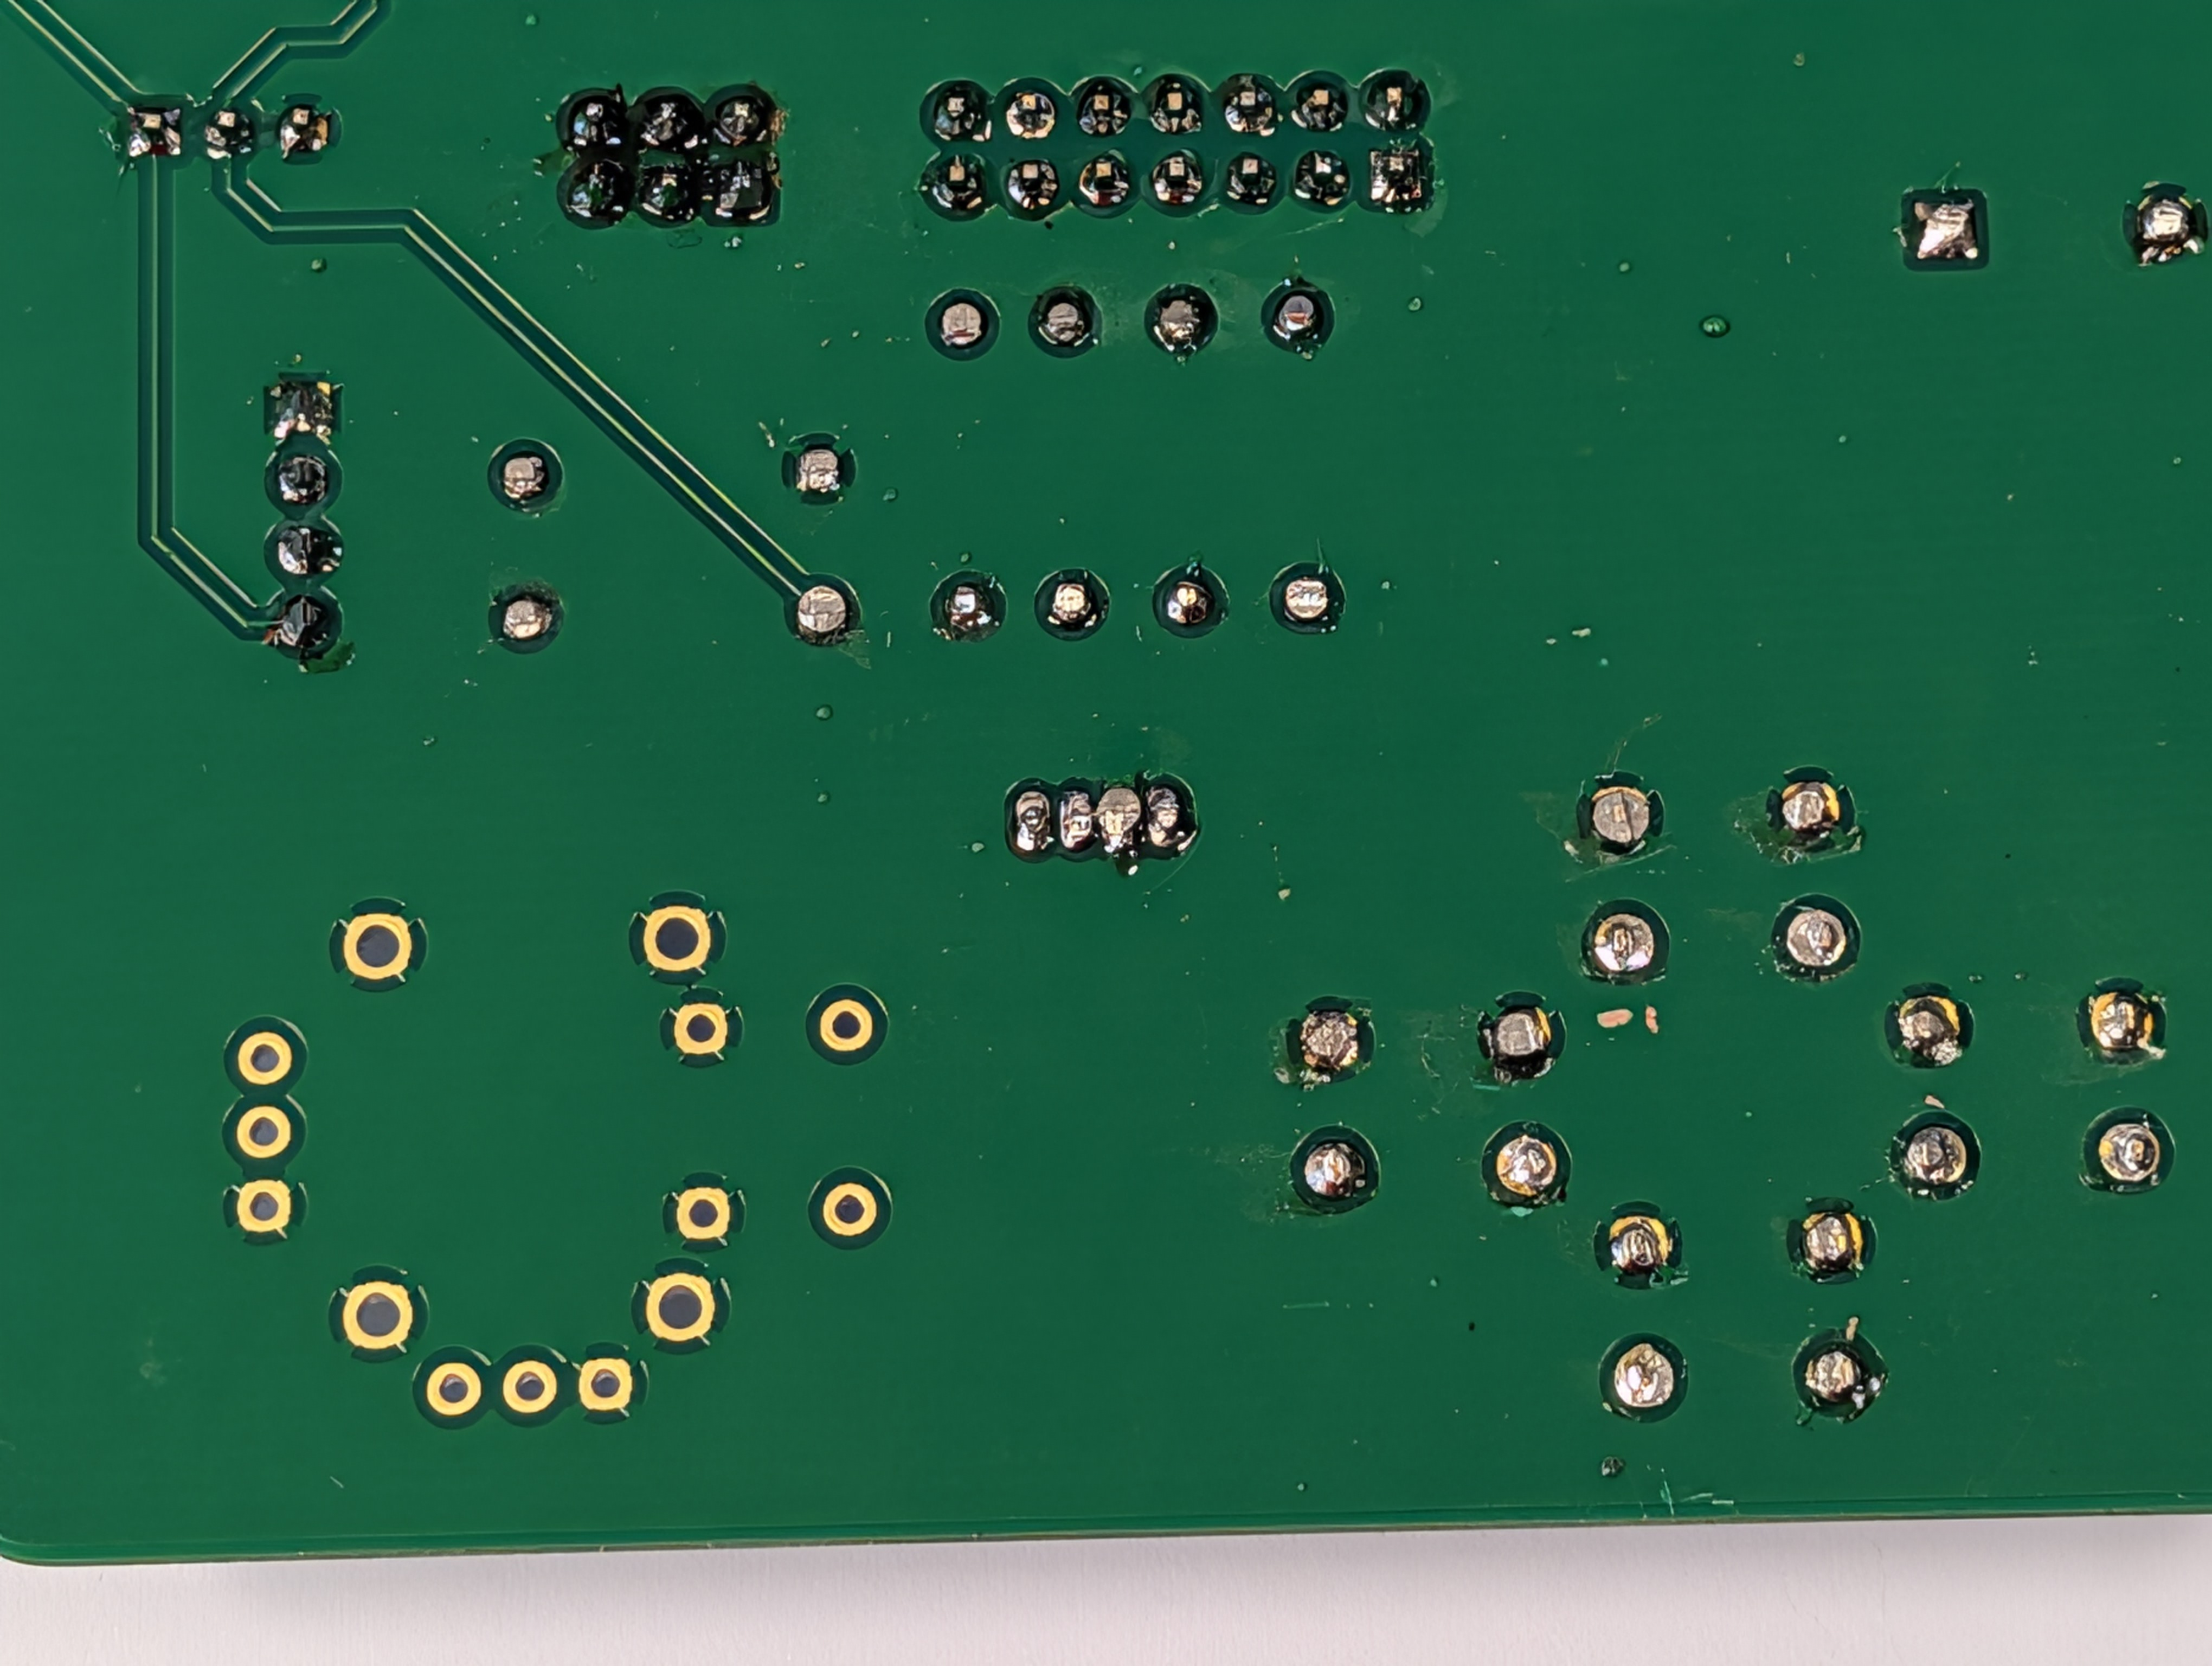
\includegraphics[width=0.75\textwidth]{pictures_of_construction/instruction_step_68.jpg}
\end{figure}

\begin{figure}[H]
    \centering
    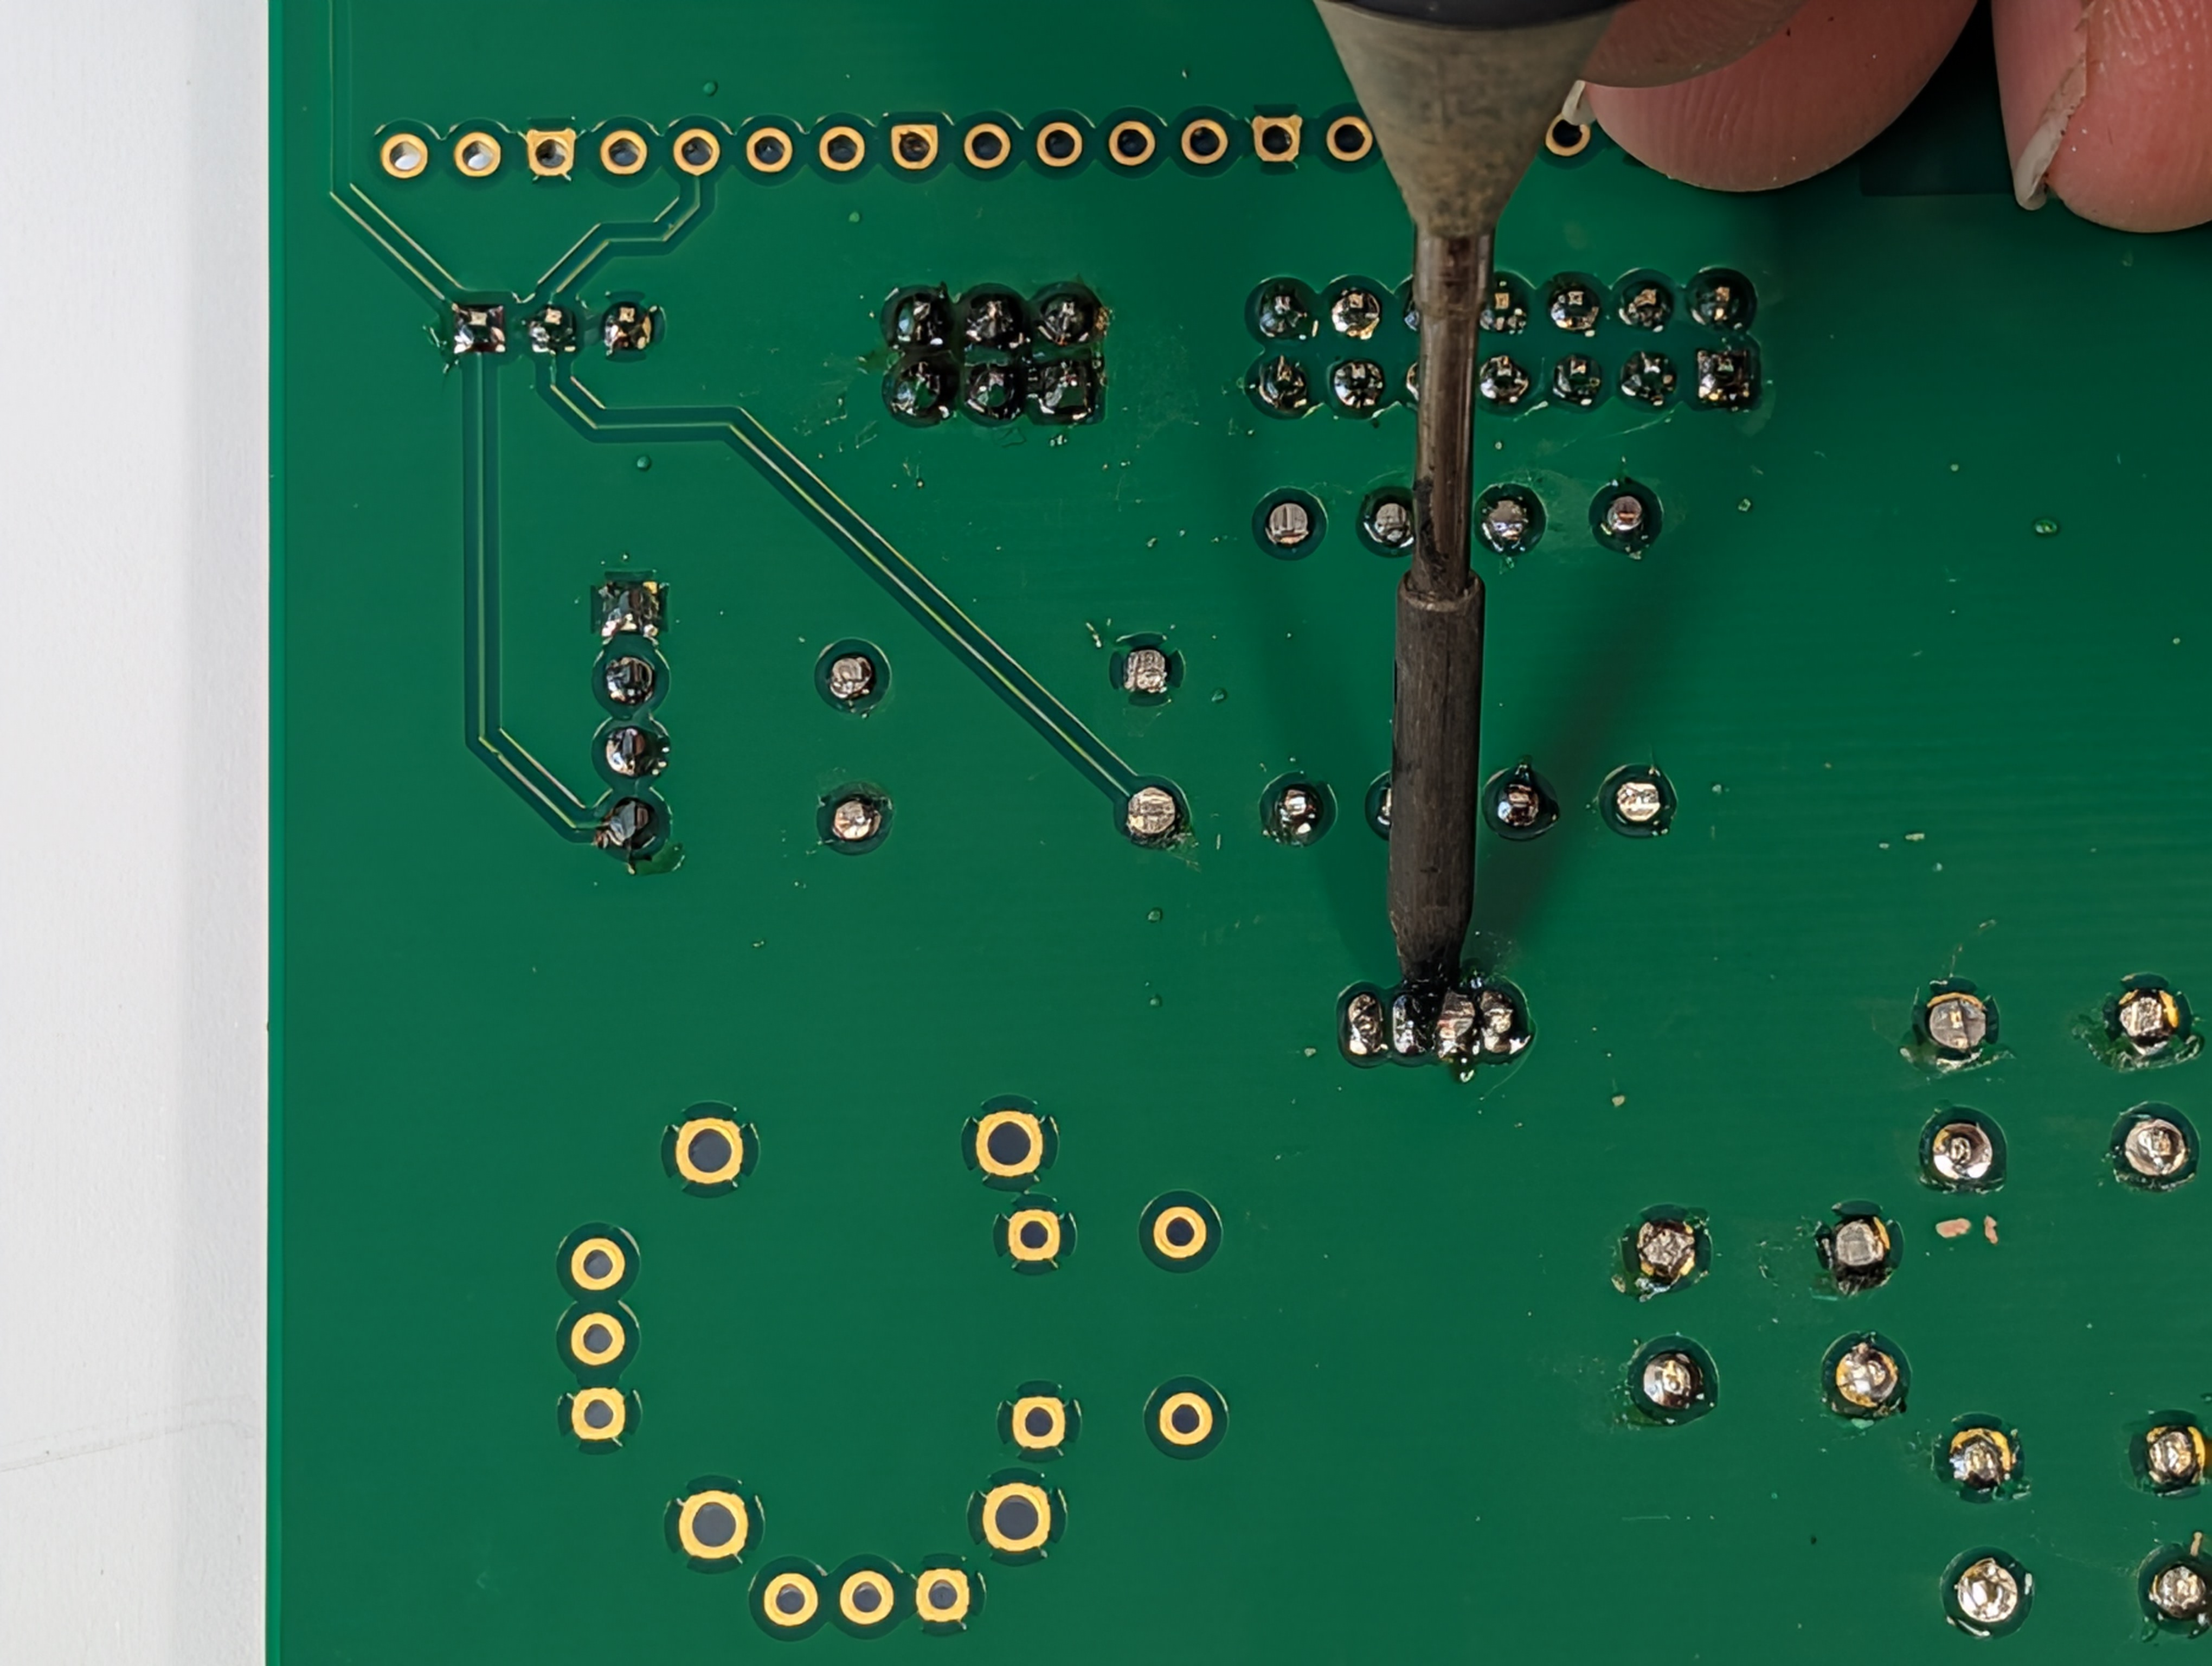
\includegraphics[width=0.75\textwidth]{pictures_of_construction/instruction_step_70.jpg}
\end{figure}

\begin{figure}[H]
    \centering
    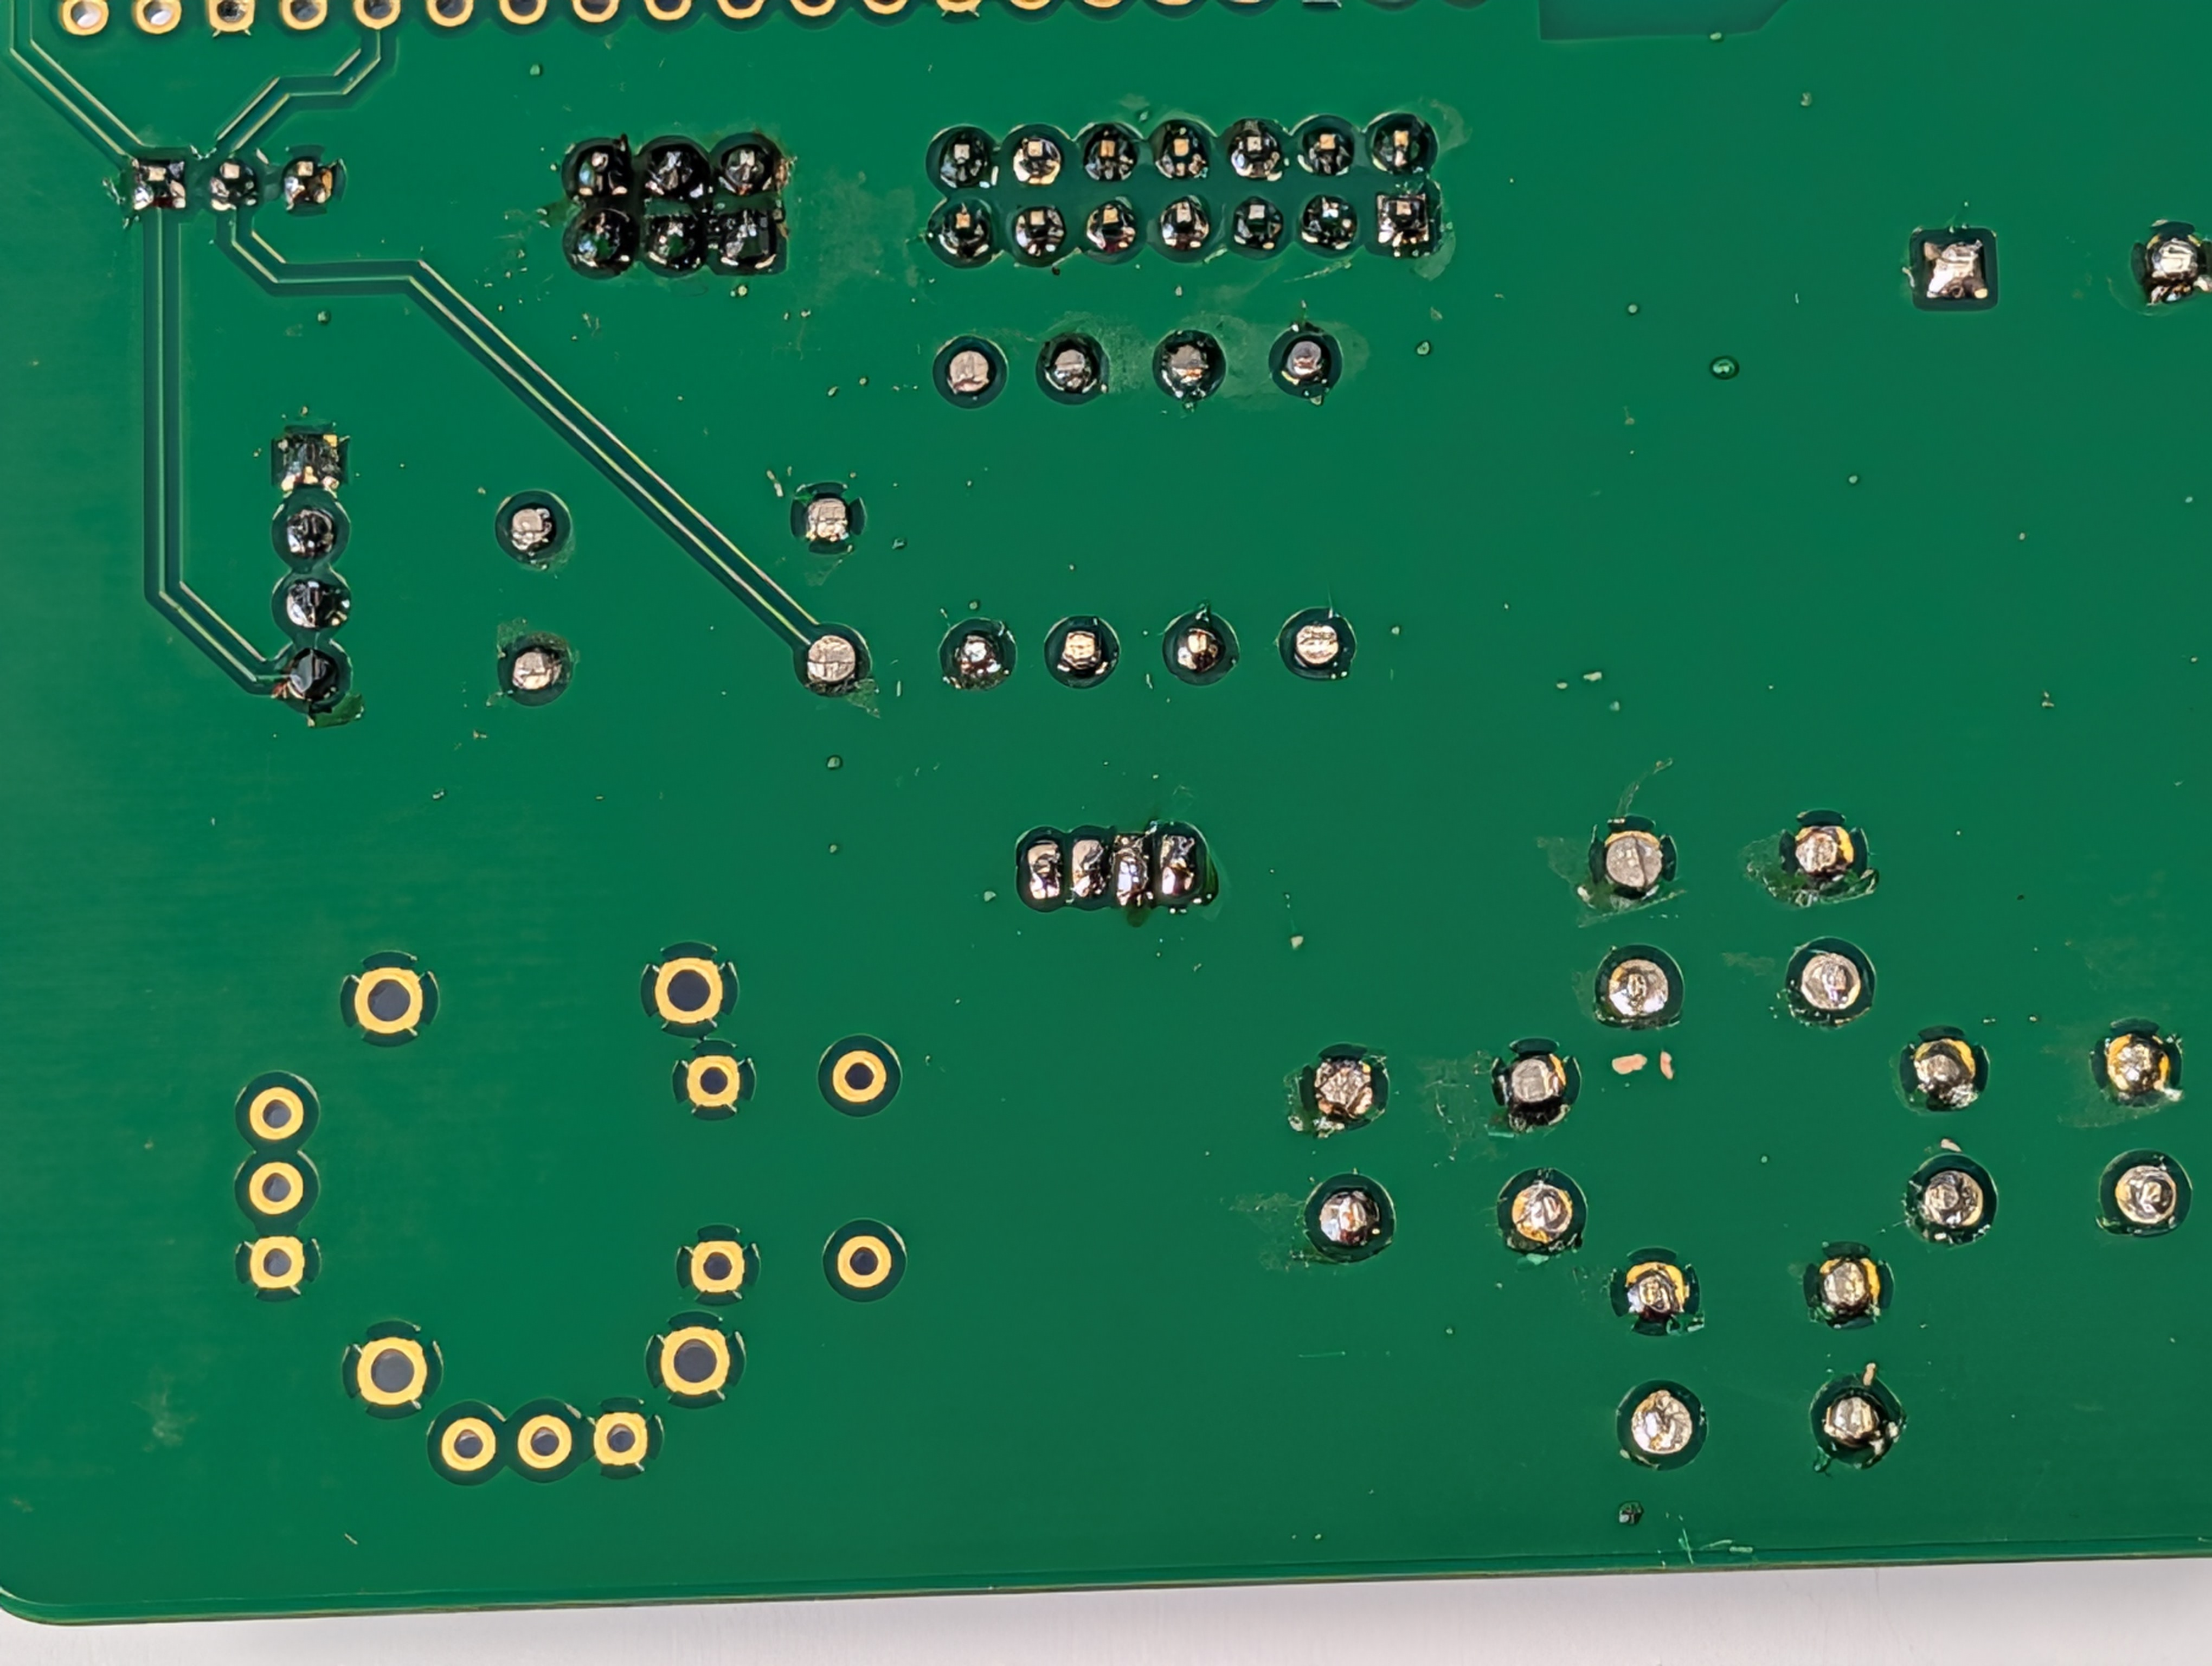
\includegraphics[width=0.75\textwidth]{pictures_of_construction/instruction_step_71.jpg}
\end{figure}

After soldering and cutting the RGB LED's leads flush, you will probably have a very ugly joint. Luckily, you can easily correct this by slowly running your soldering iron between two pins and letting them reflow. The surface tension of the solder should pull the joint nicely together, resulting in a clean joint. But check for any bridges after that. If there are any, clean your soldering tip and repeat the reflow.

\subsection*{Installation of the Raspberry Pi Pico}

\begin{figure}[H]
    \centering
    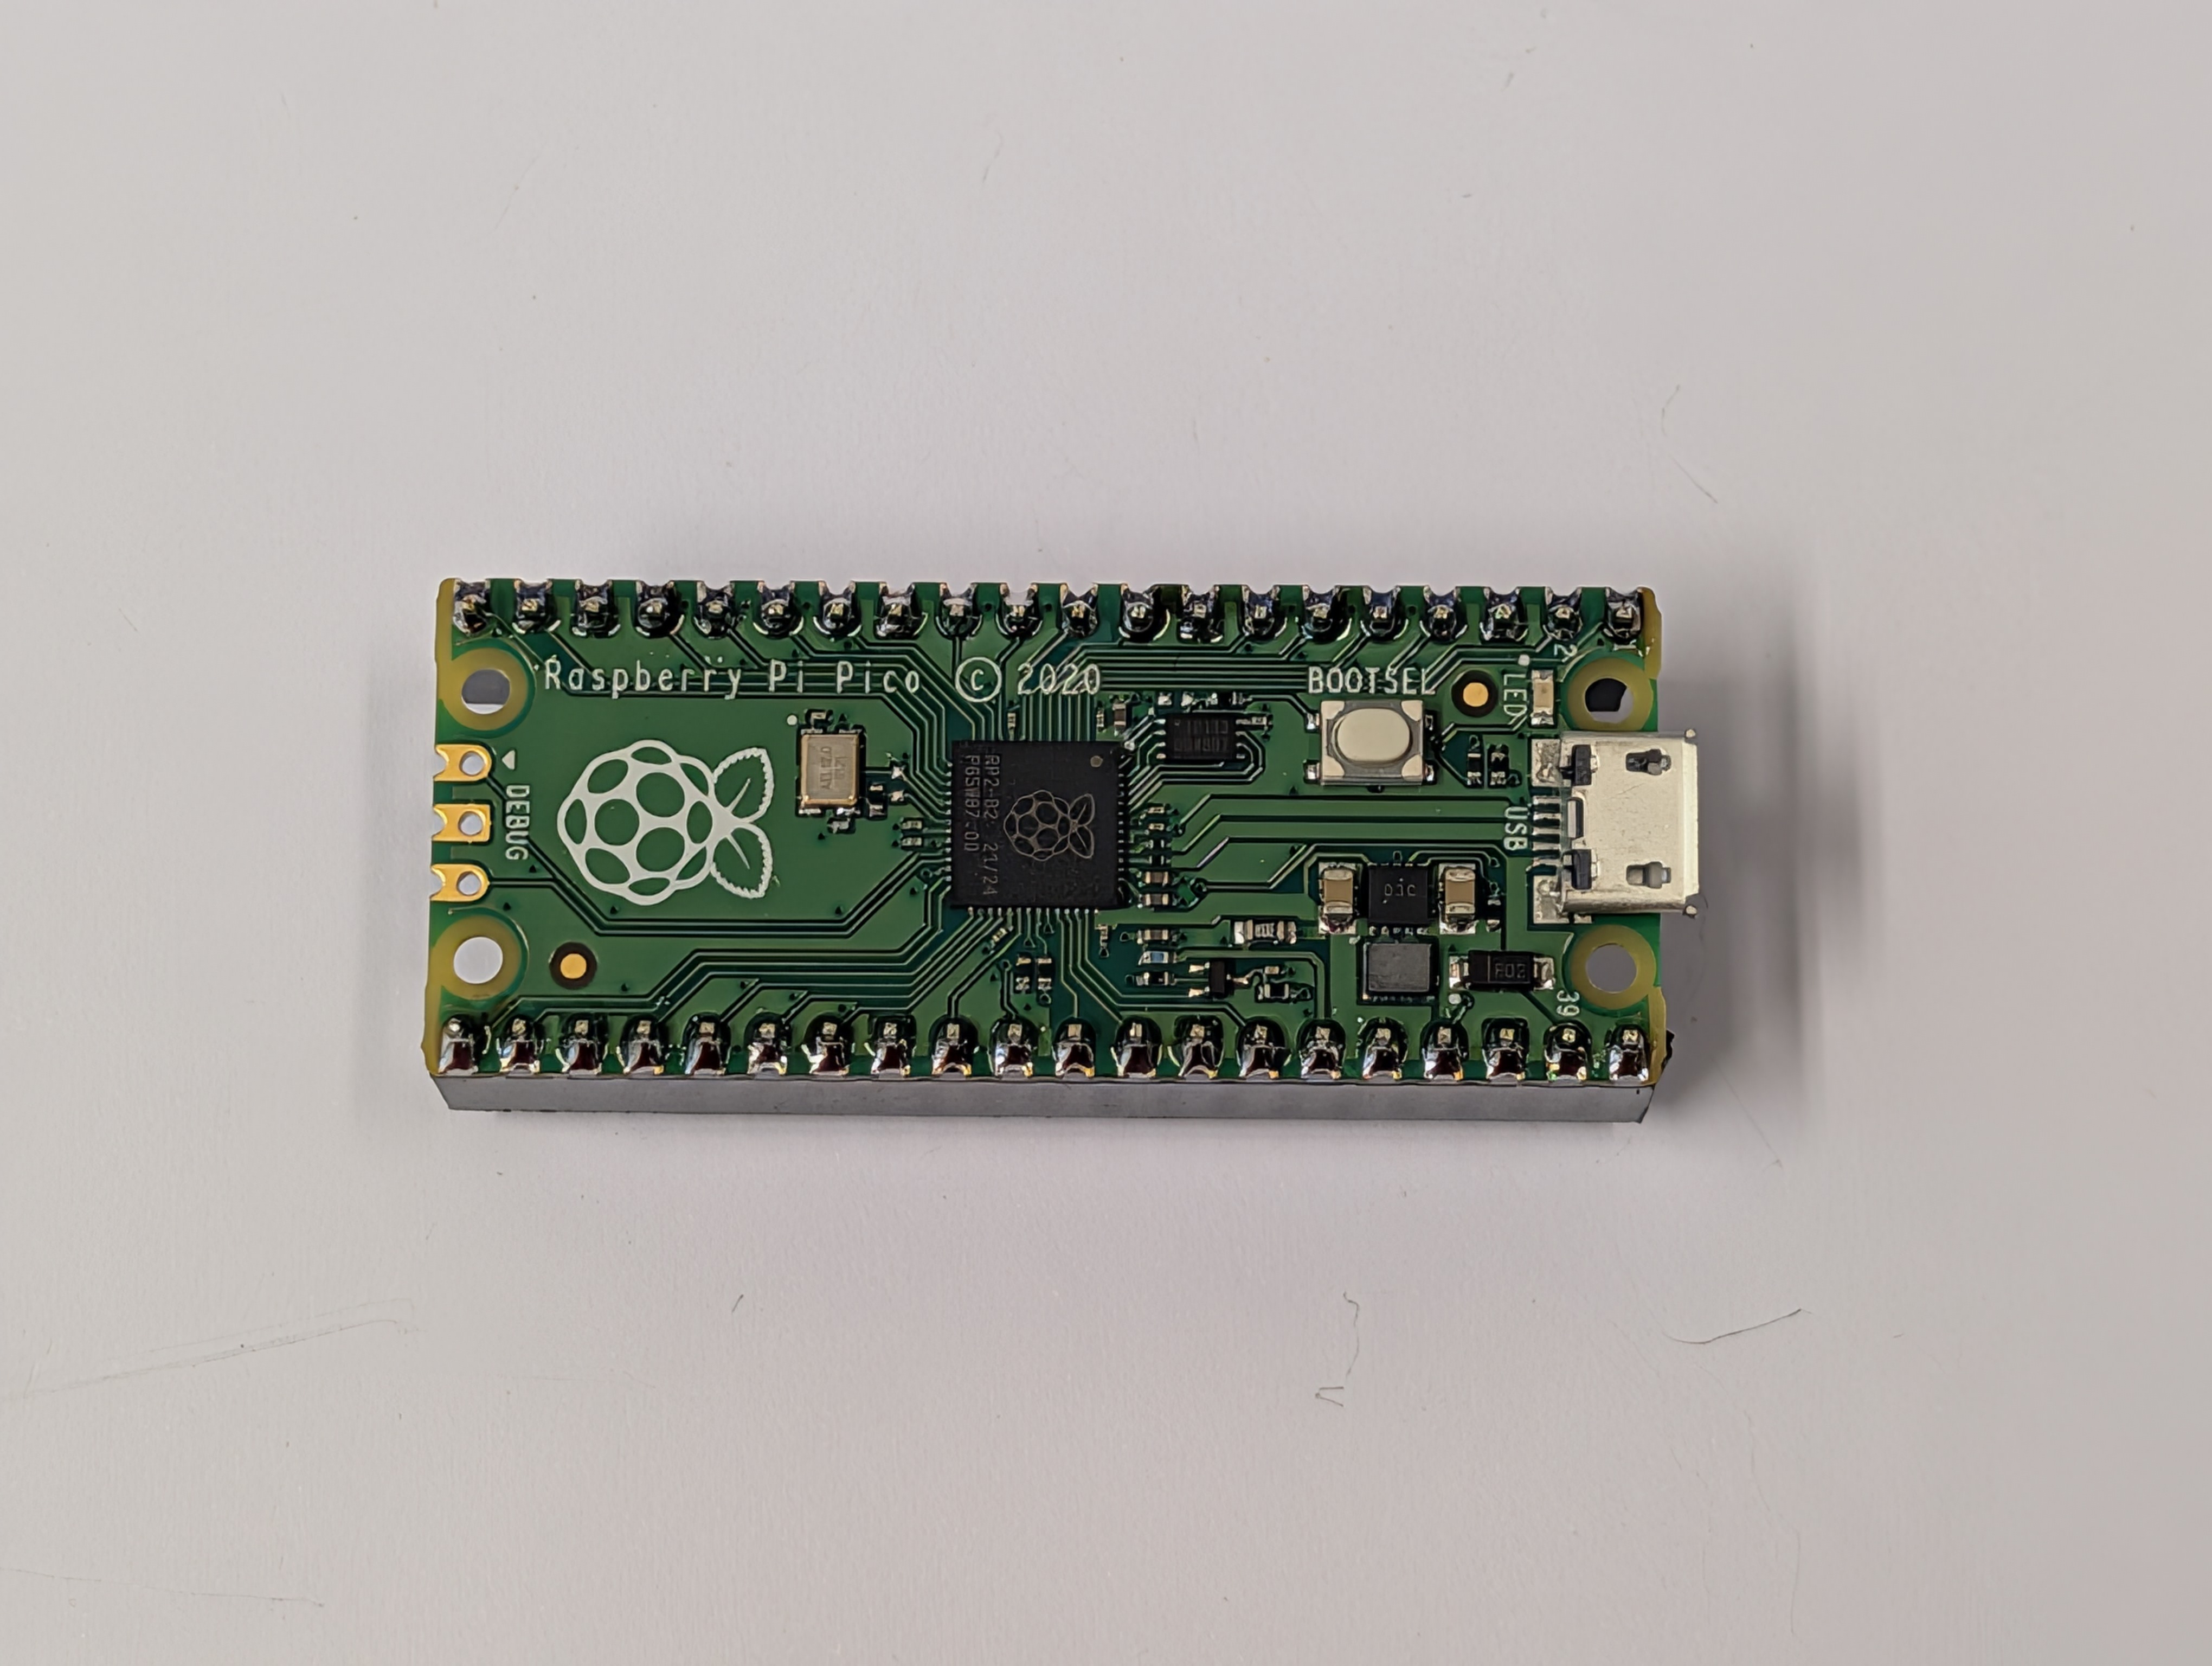
\includegraphics[width=0.75\textwidth]{pictures_of_construction/instruction_step_72.jpg}
\end{figure}

\begin{figure}[H]
    \centering
    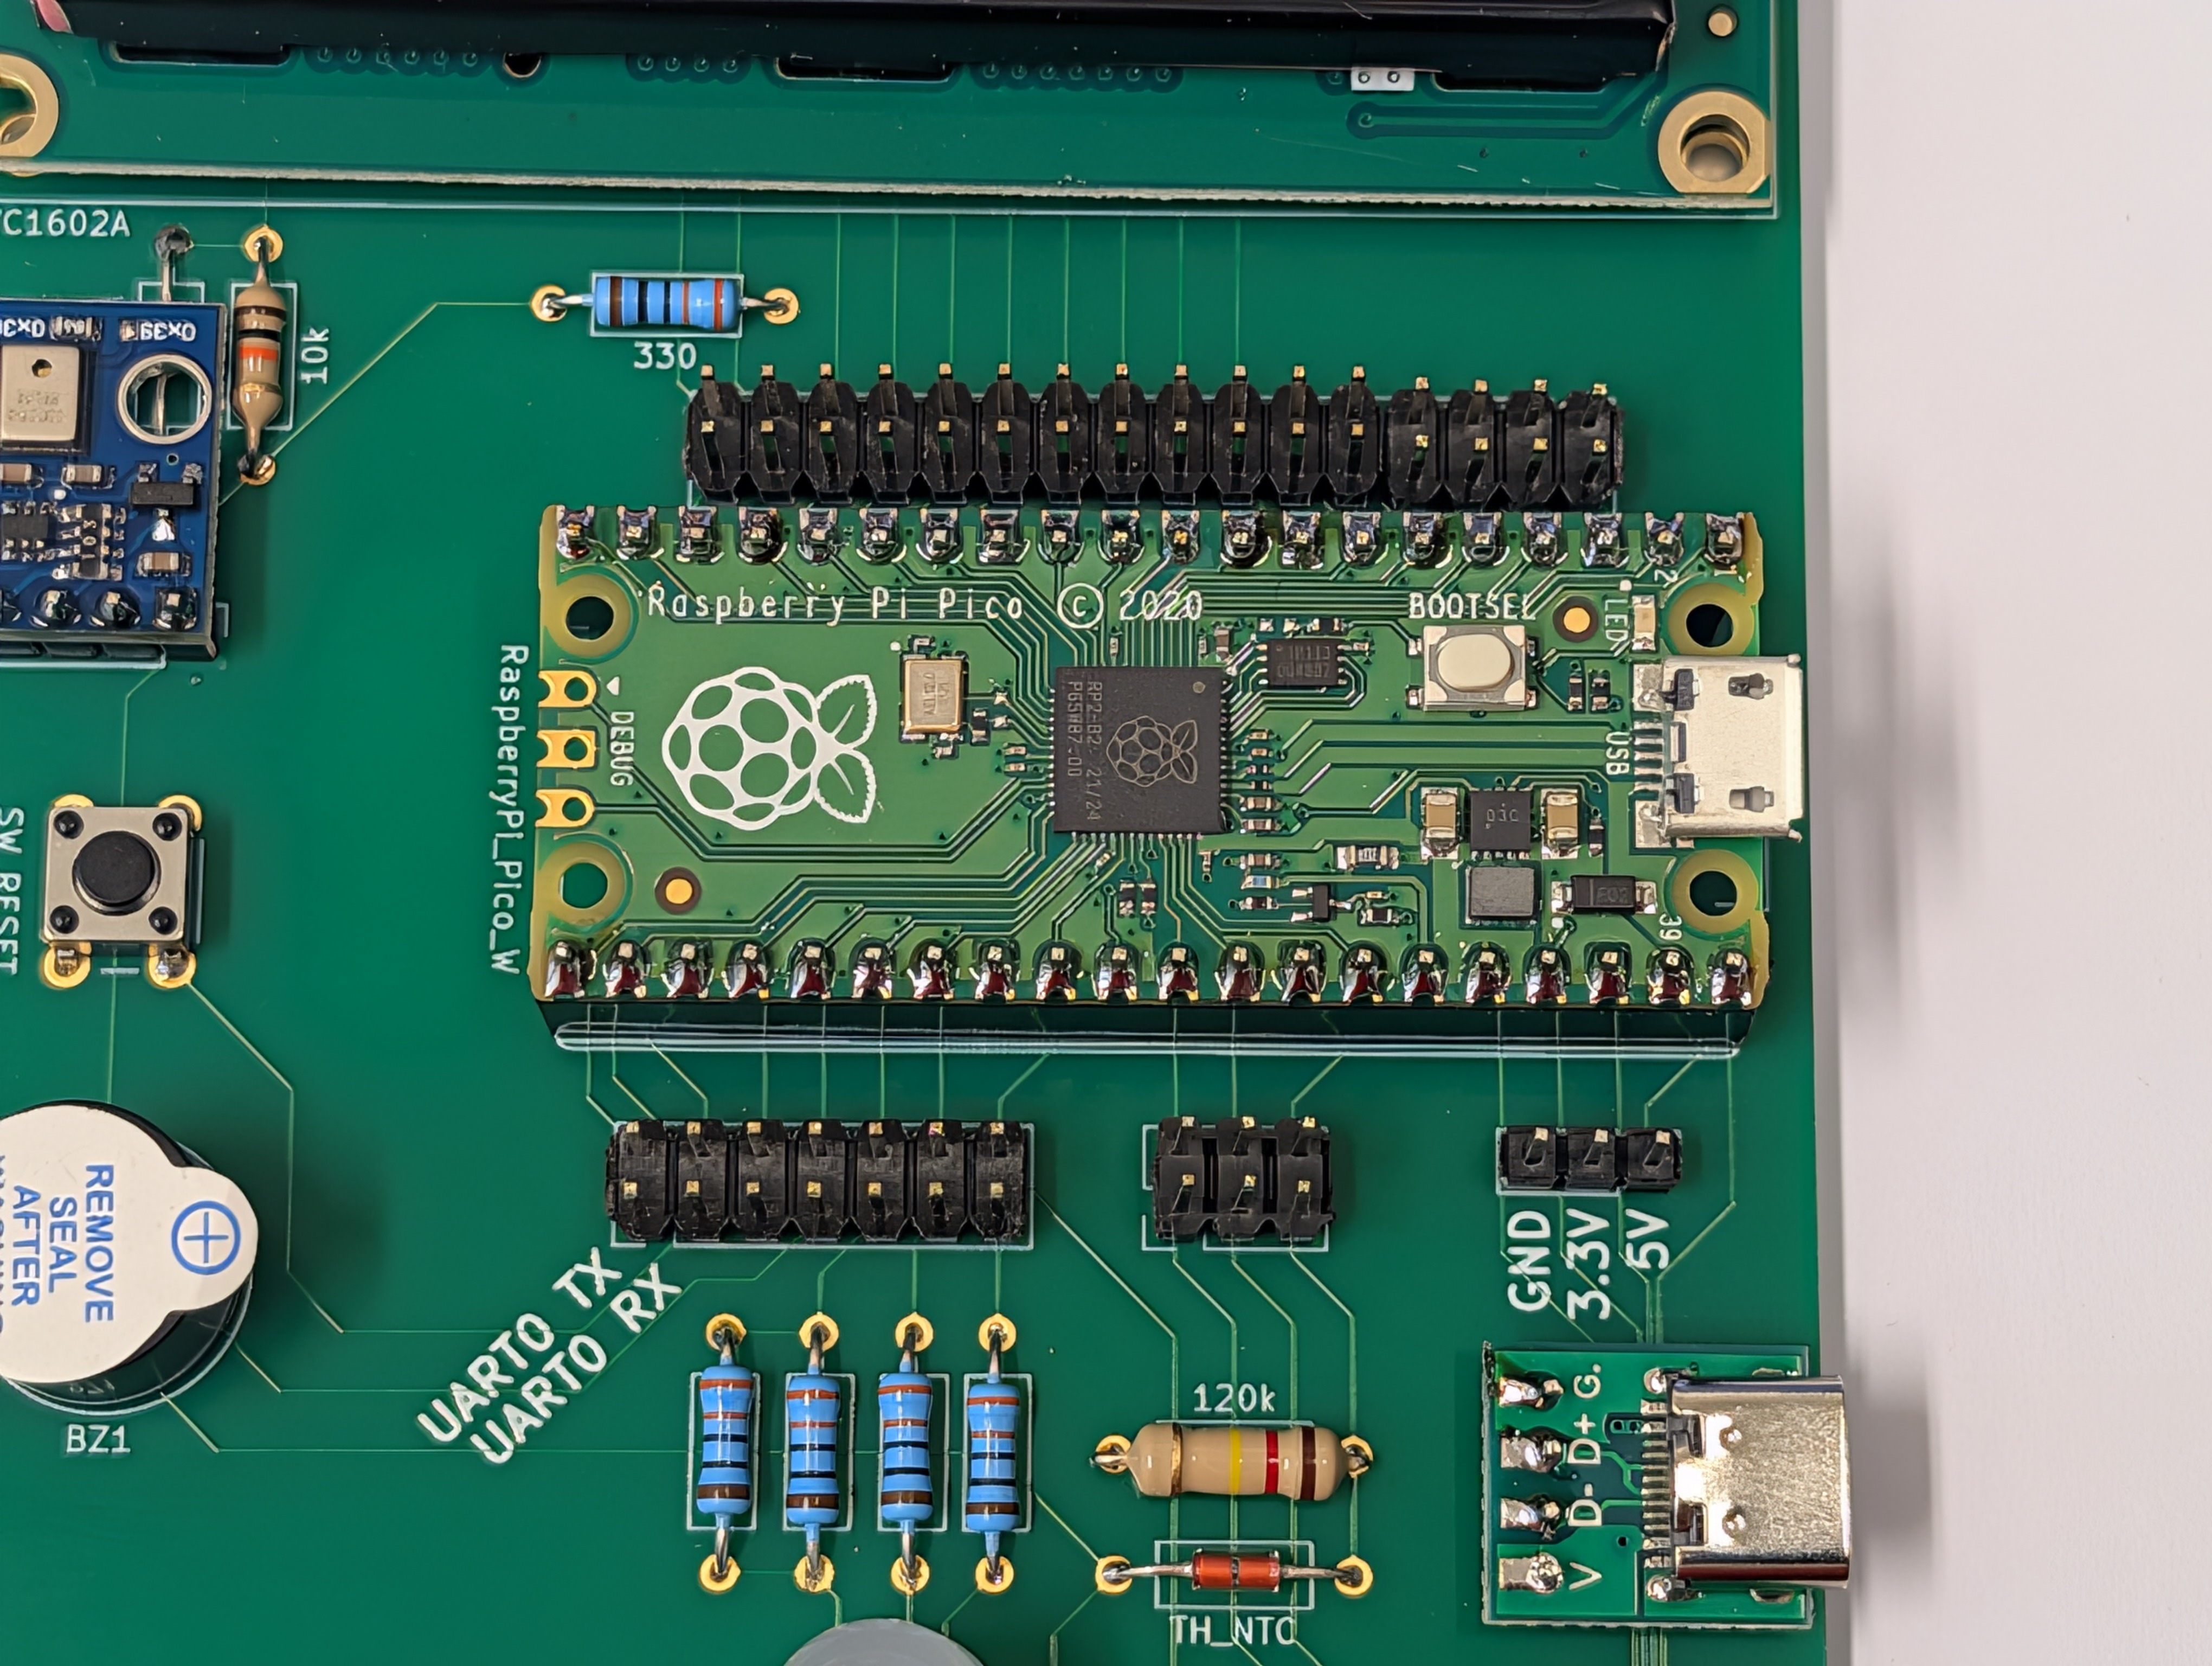
\includegraphics[width=0.75\textwidth]{pictures_of_construction/instruction_step_73.jpg}
\end{figure}

\begin{figure}[H]
    \centering
    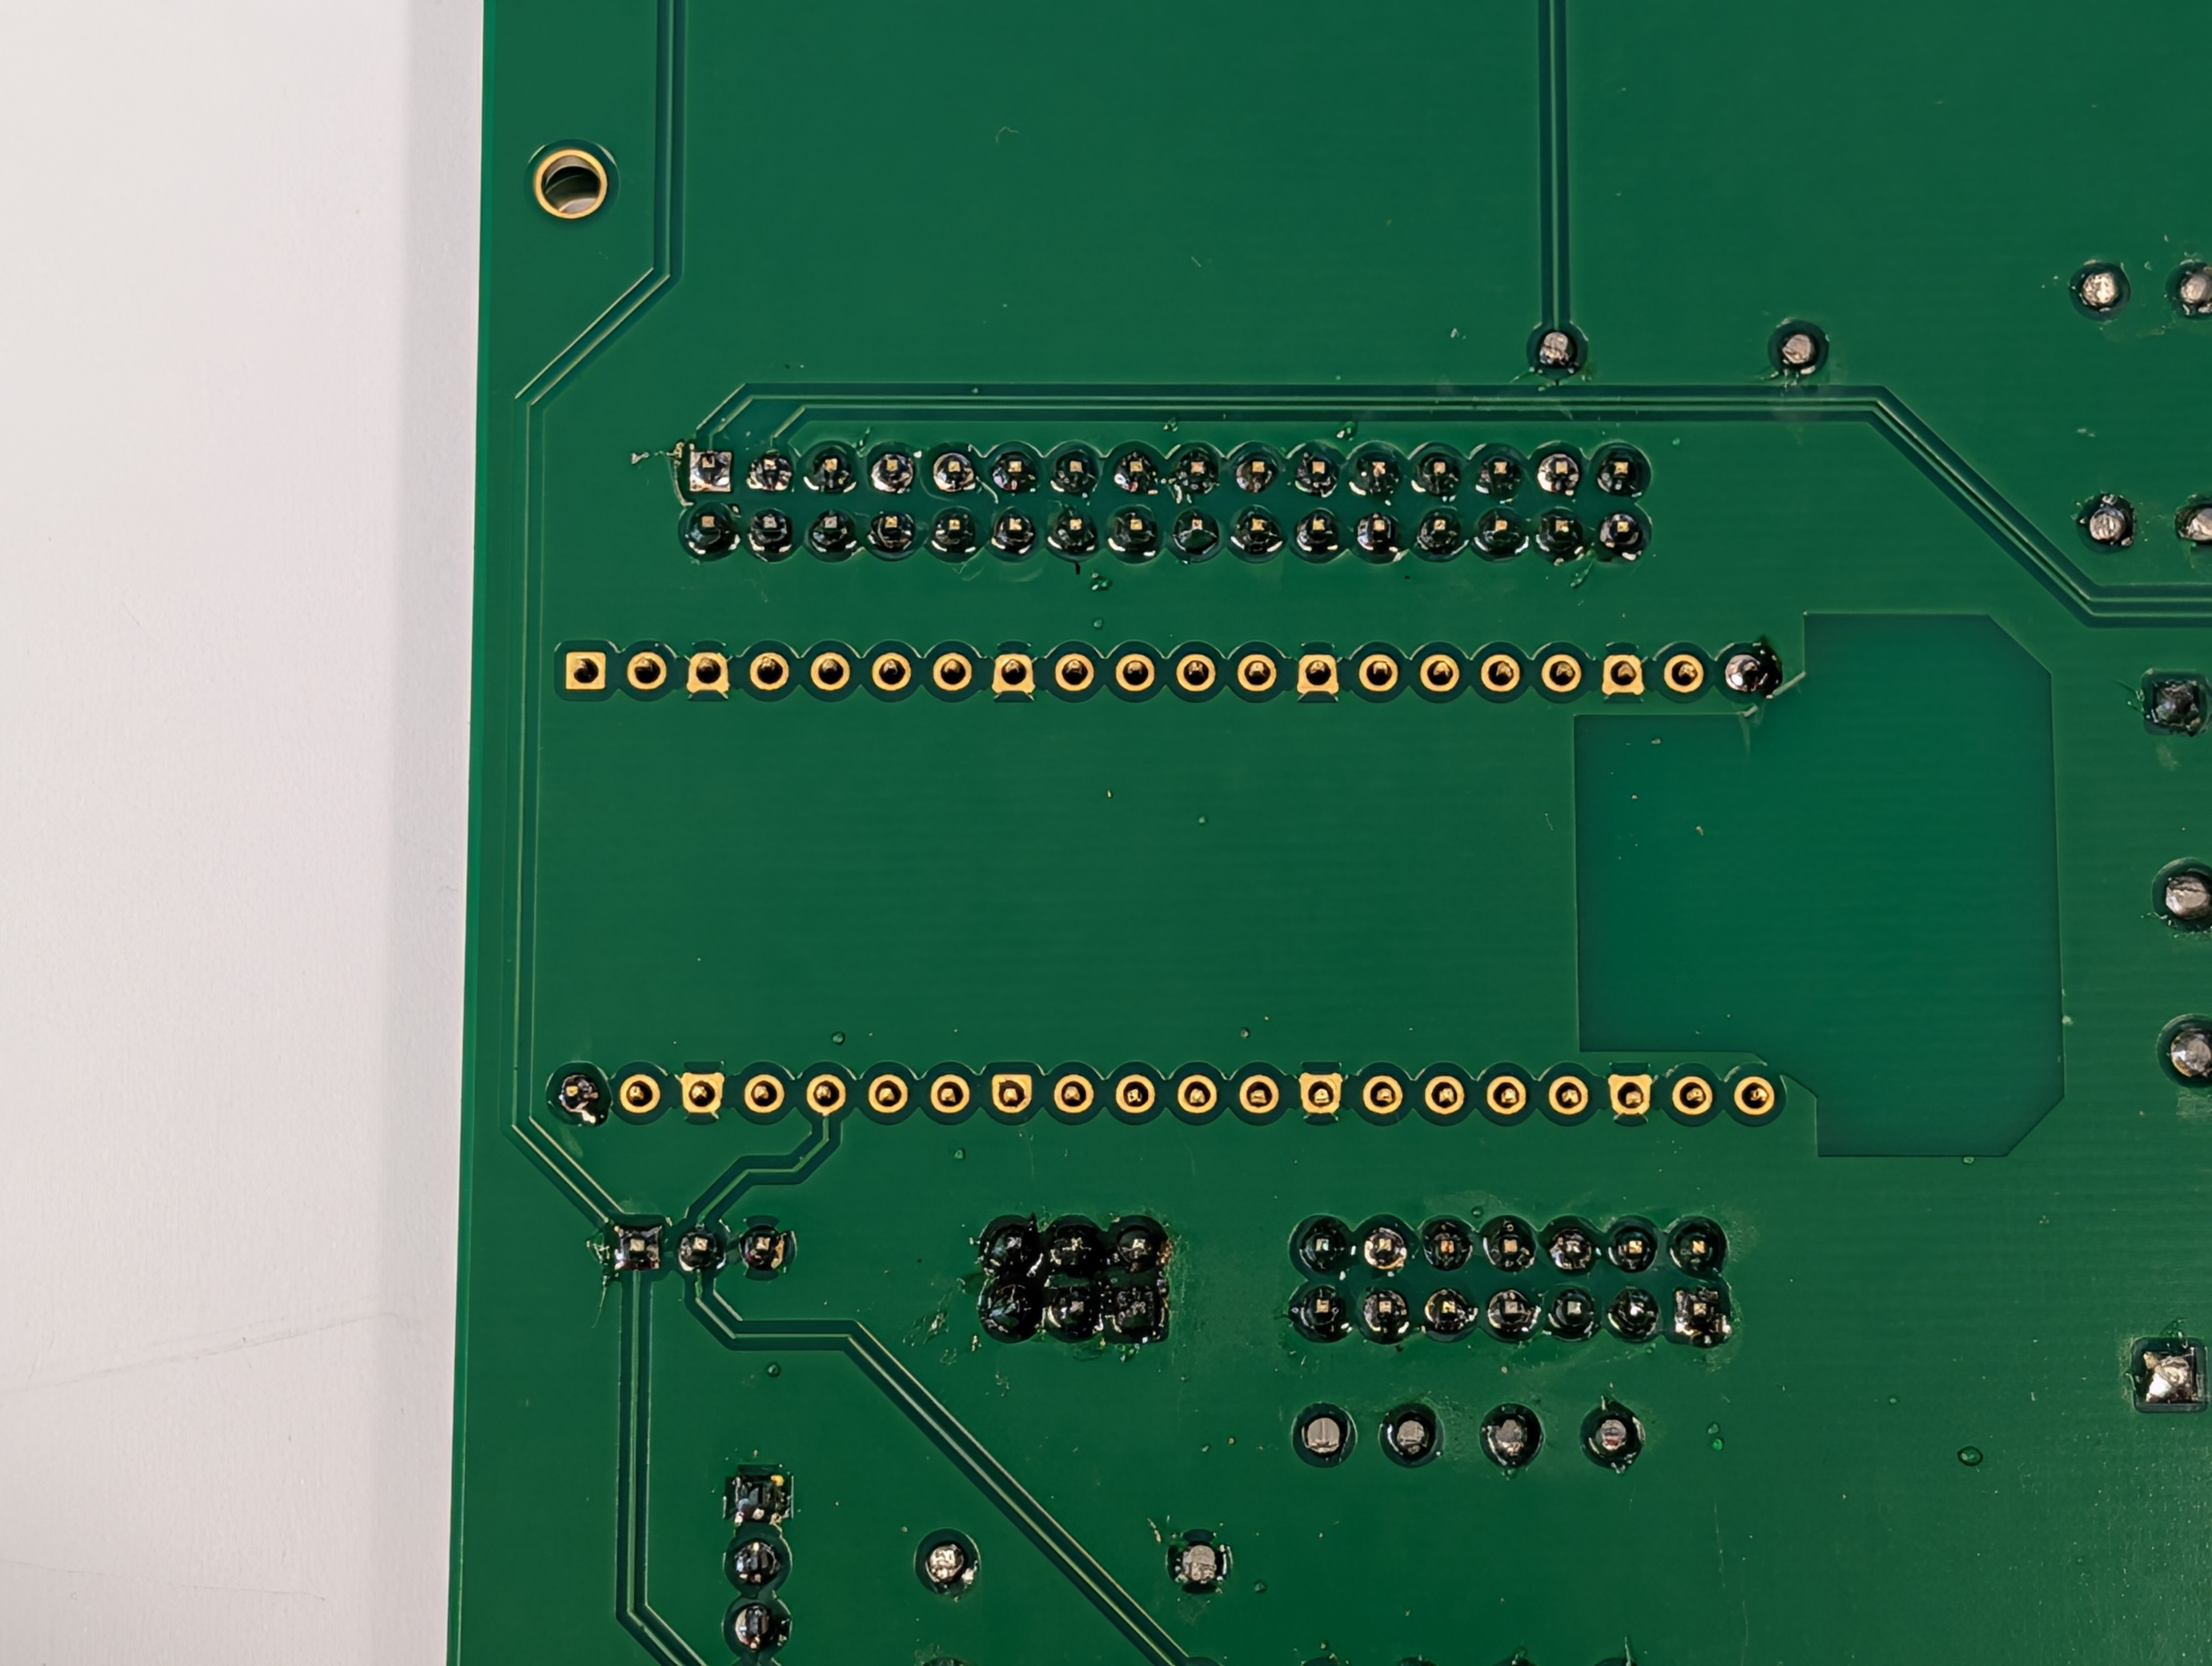
\includegraphics[width=0.75\textwidth]{pictures_of_construction/instruction_step_74.jpg}
\end{figure}

Now we can install the Raspberry Pi Pico. As with all previous complex connections, start by soldering only two opposite pins. Then check for alignment; after that, solder completely.

\subsection*{Installation of the analogue joystick}

\begin{figure}[H]
    \centering
    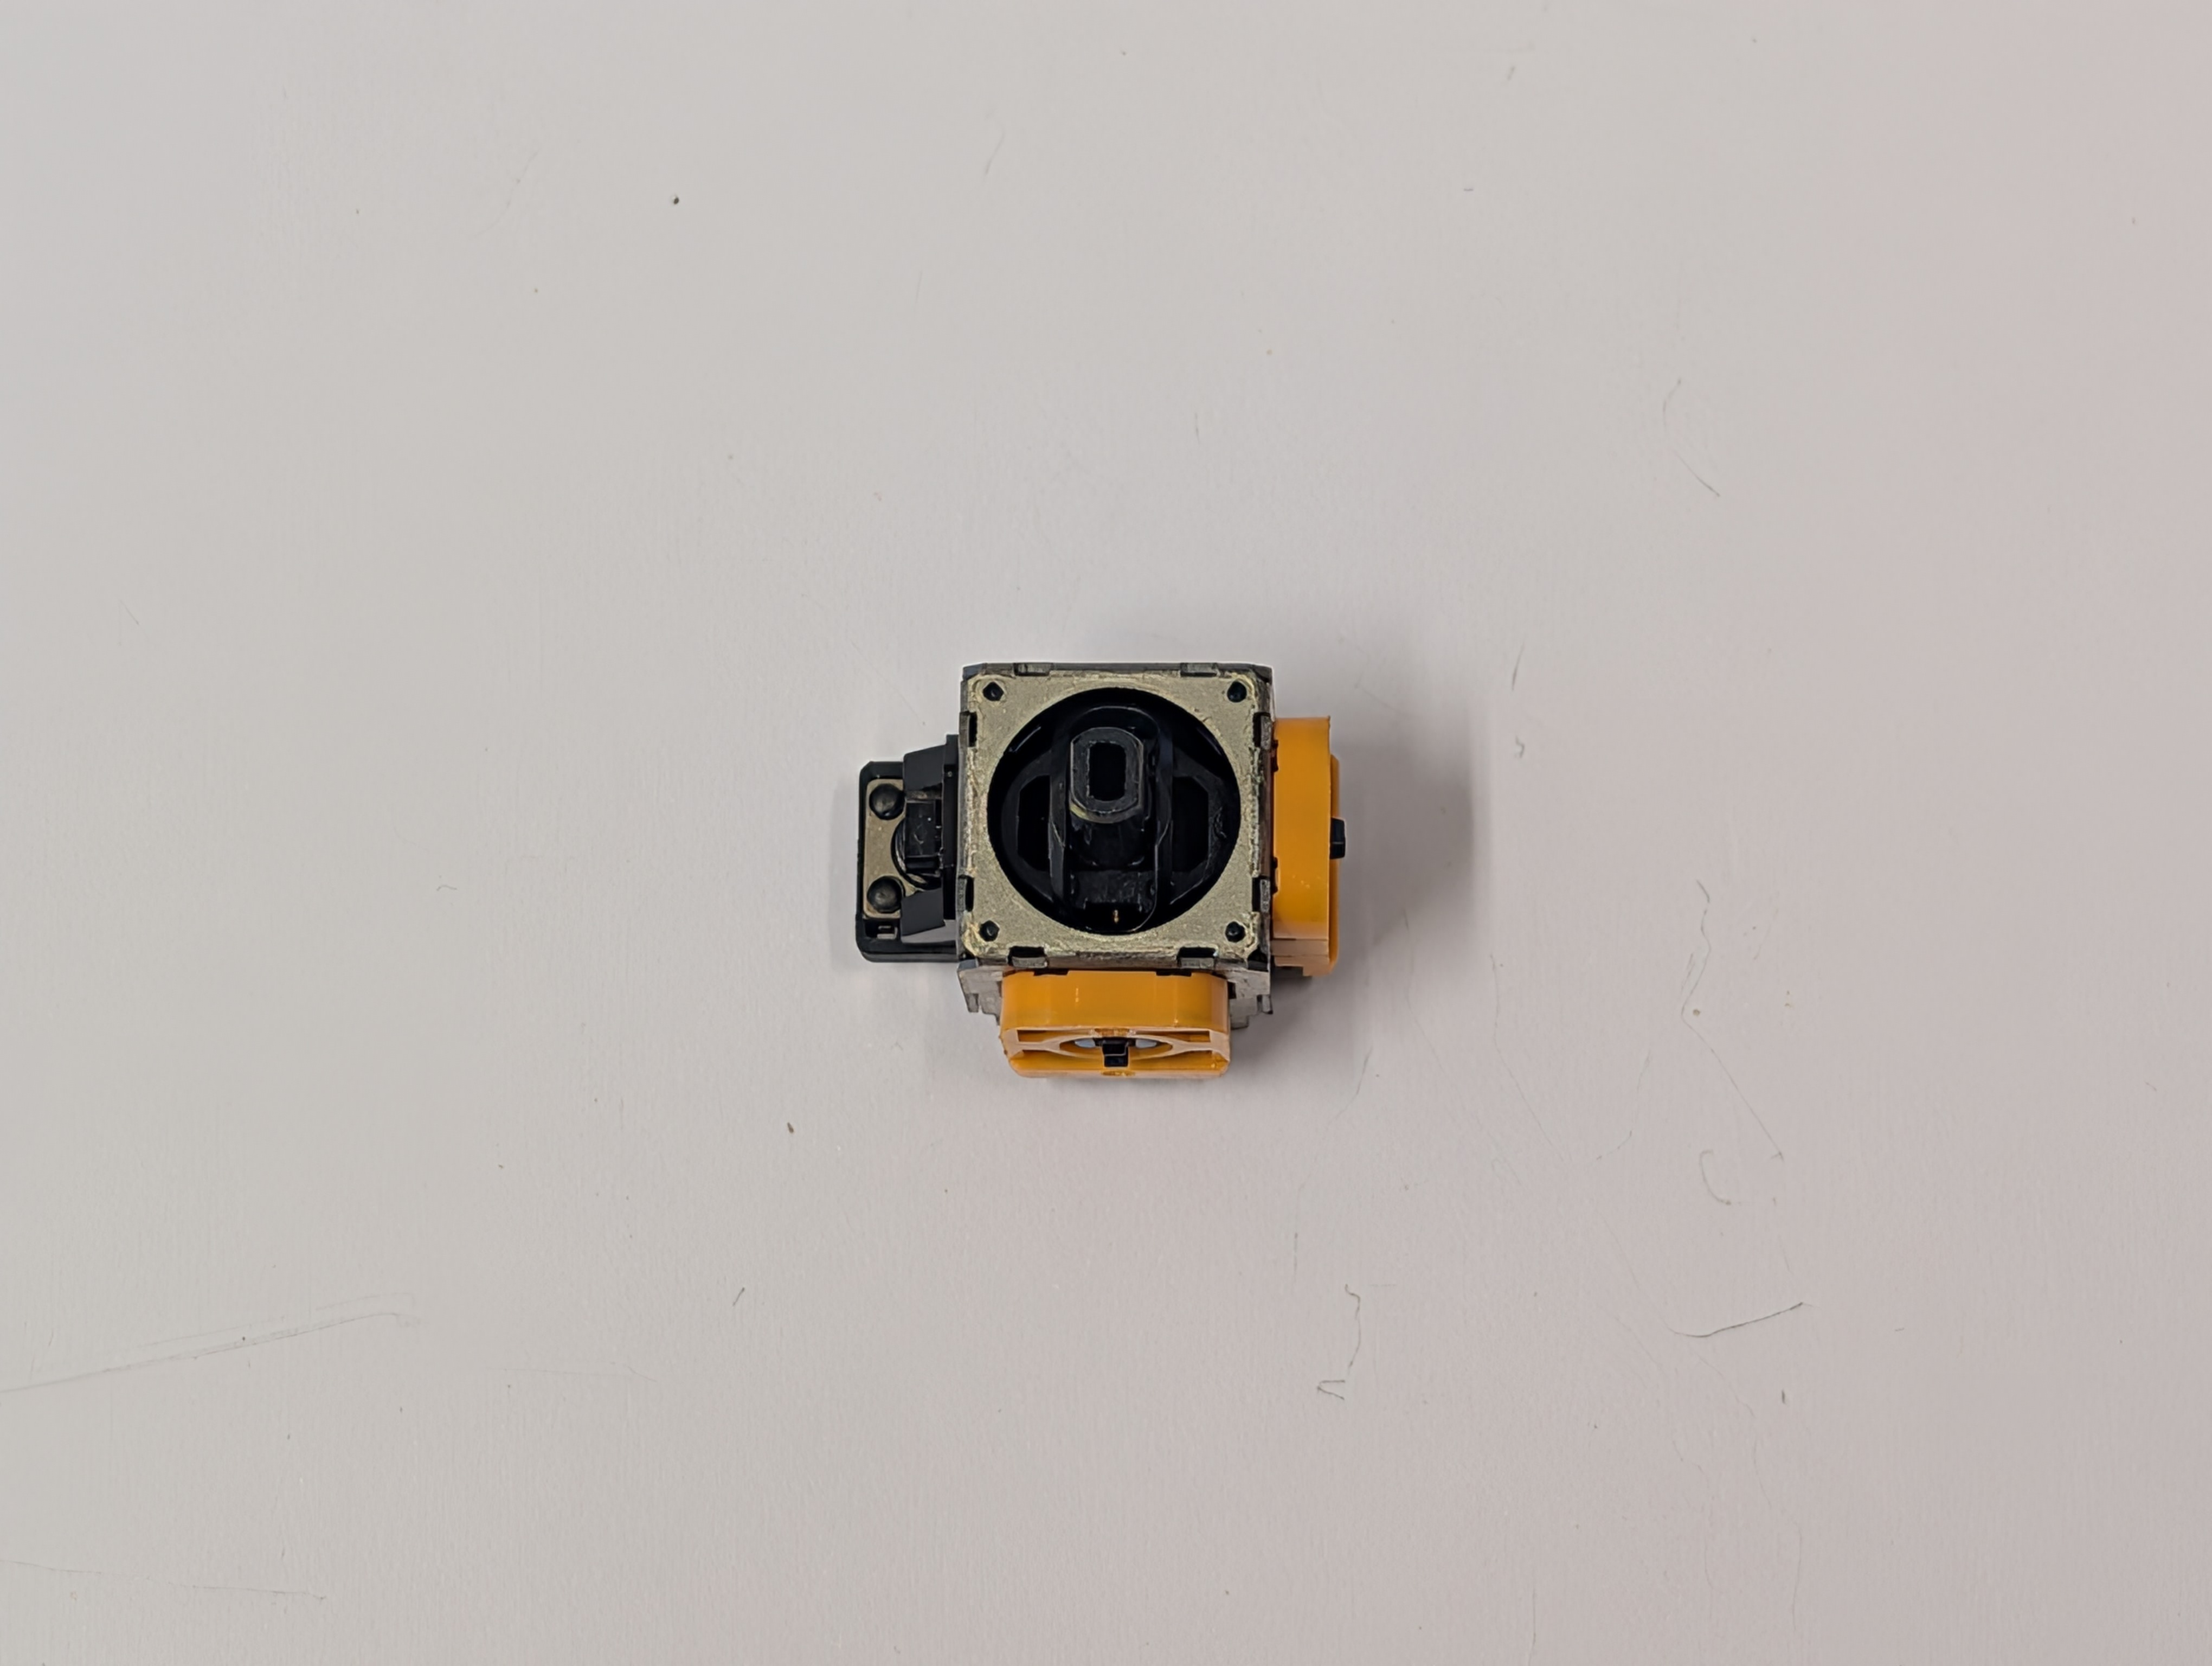
\includegraphics[width=0.75\textwidth]{pictures_of_construction/instruction_step_75.jpg}
\end{figure}

\begin{figure}[H]
    \centering
    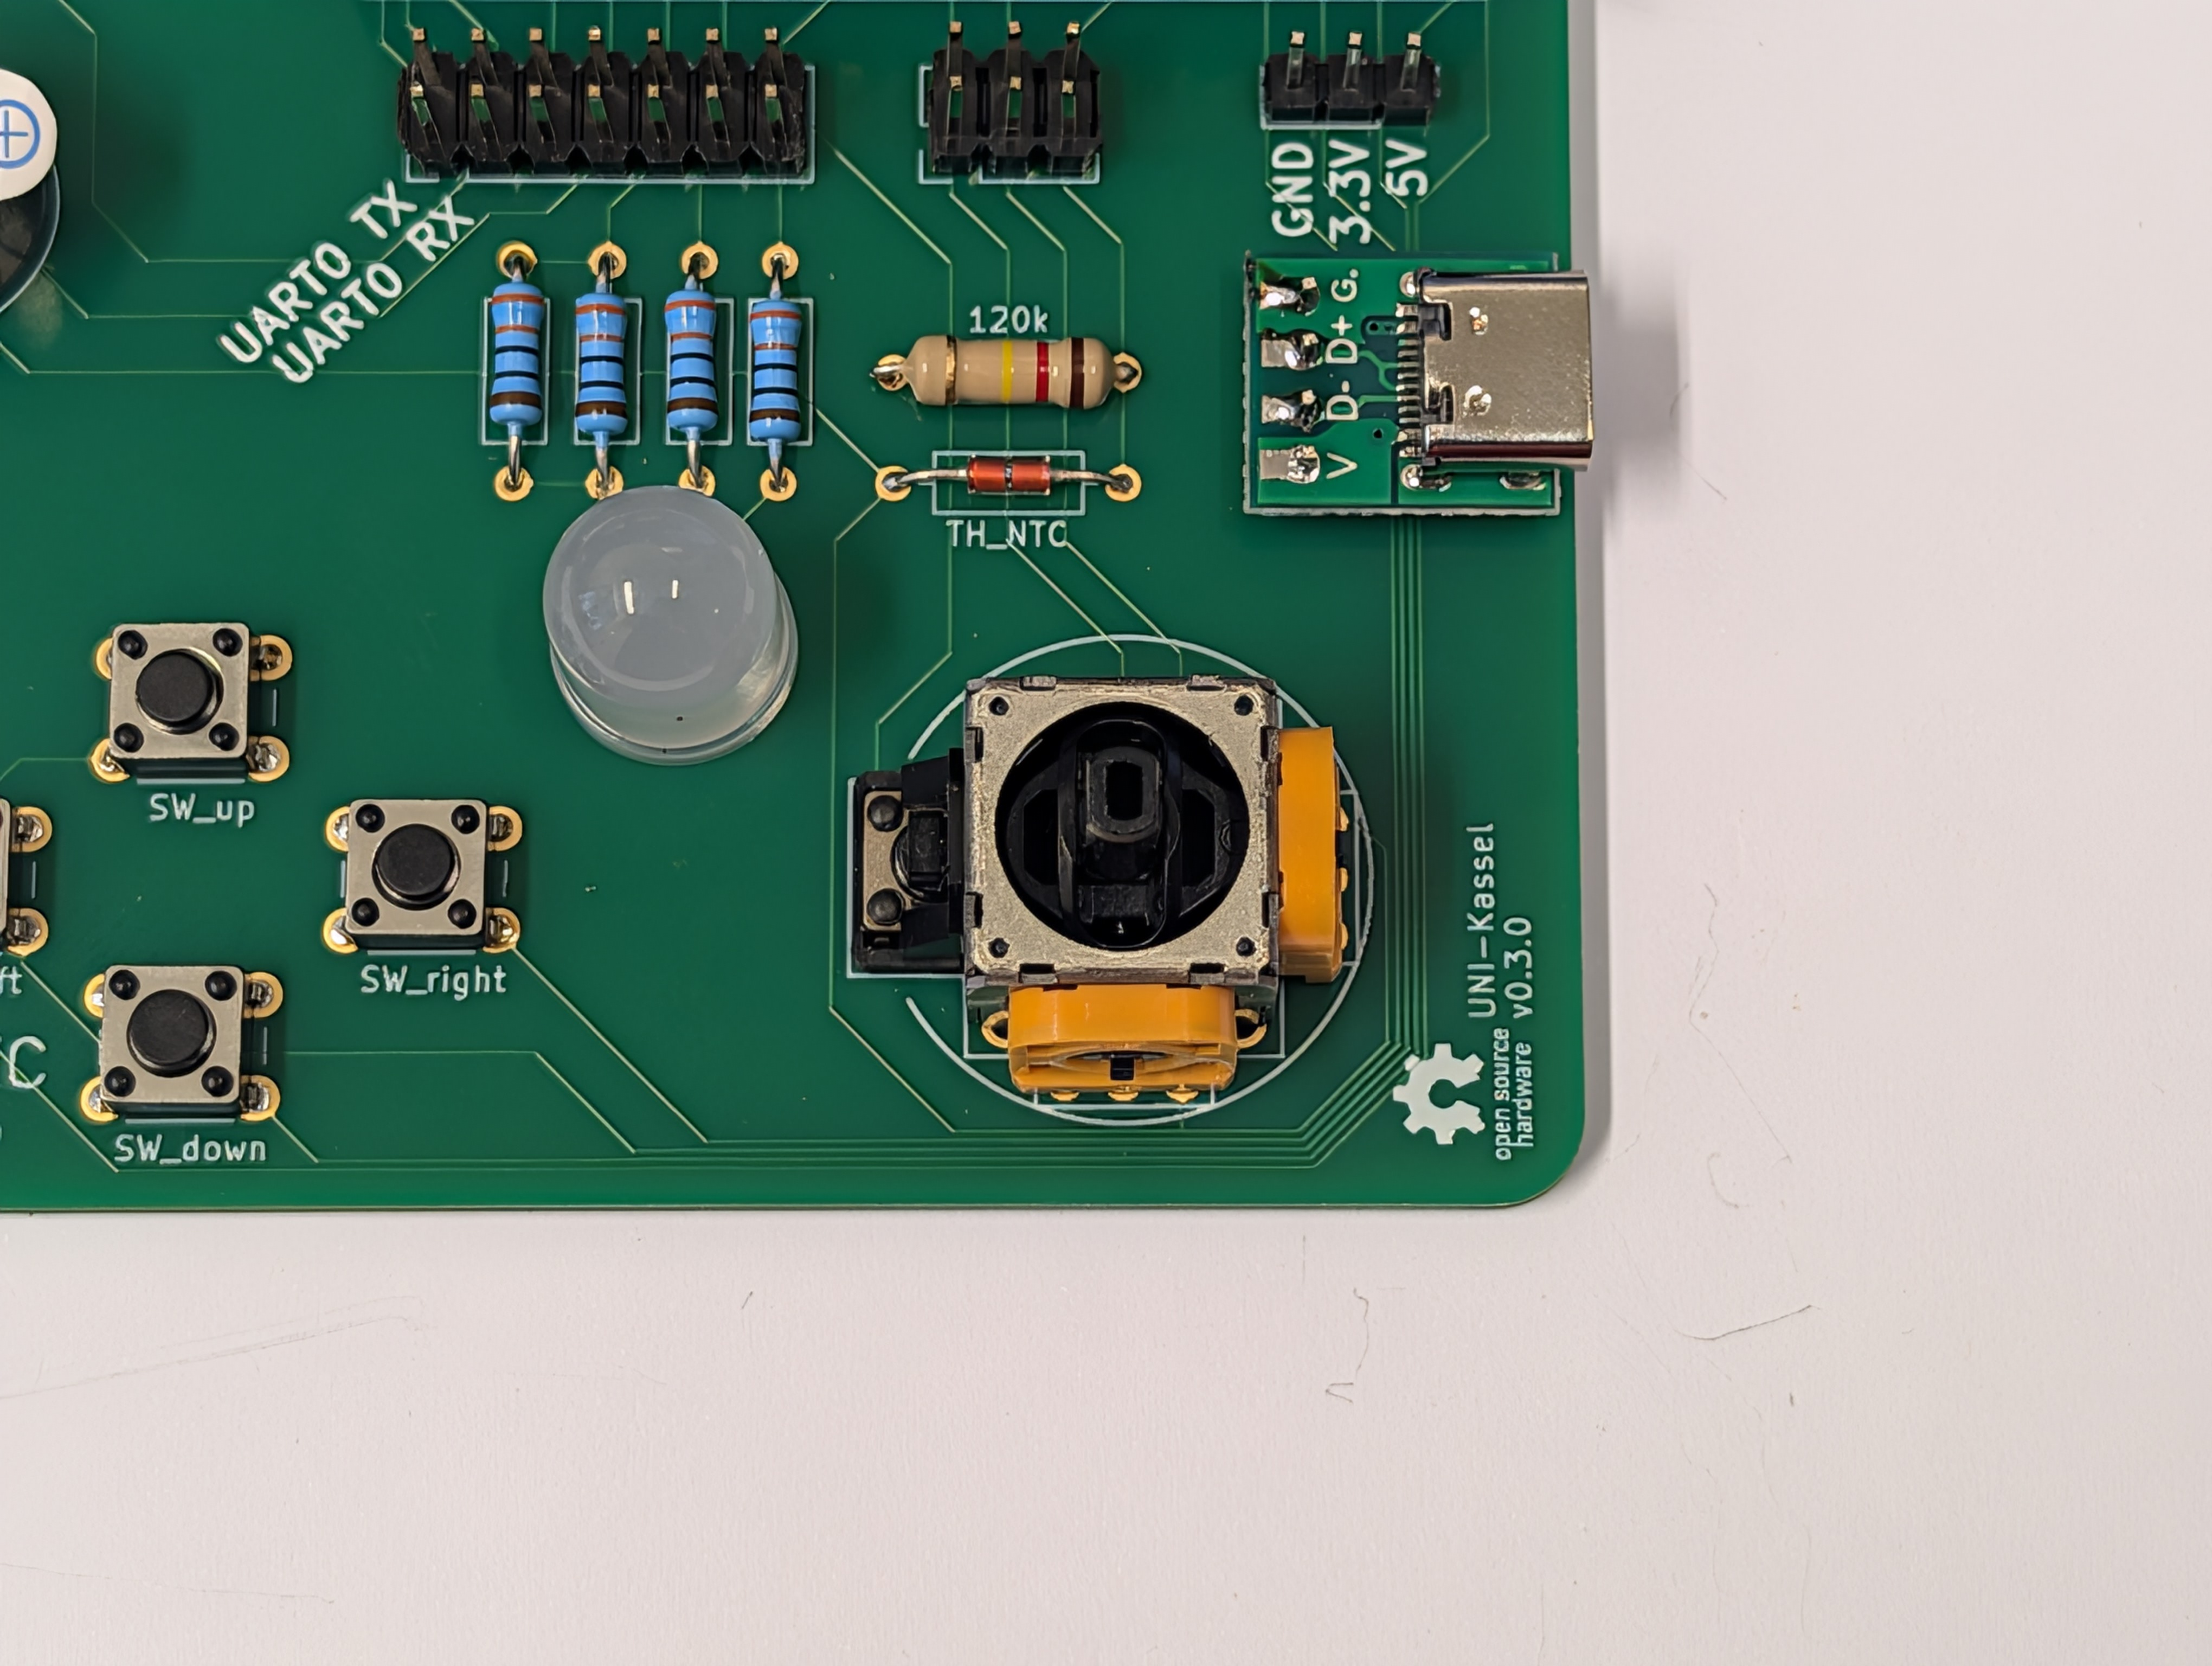
\includegraphics[width=0.75\textwidth]{pictures_of_construction/instruction_step_76.jpg}
\end{figure}

As the last component, we will install the analogue joystick.

\begin{figure}[H]
    \centering
    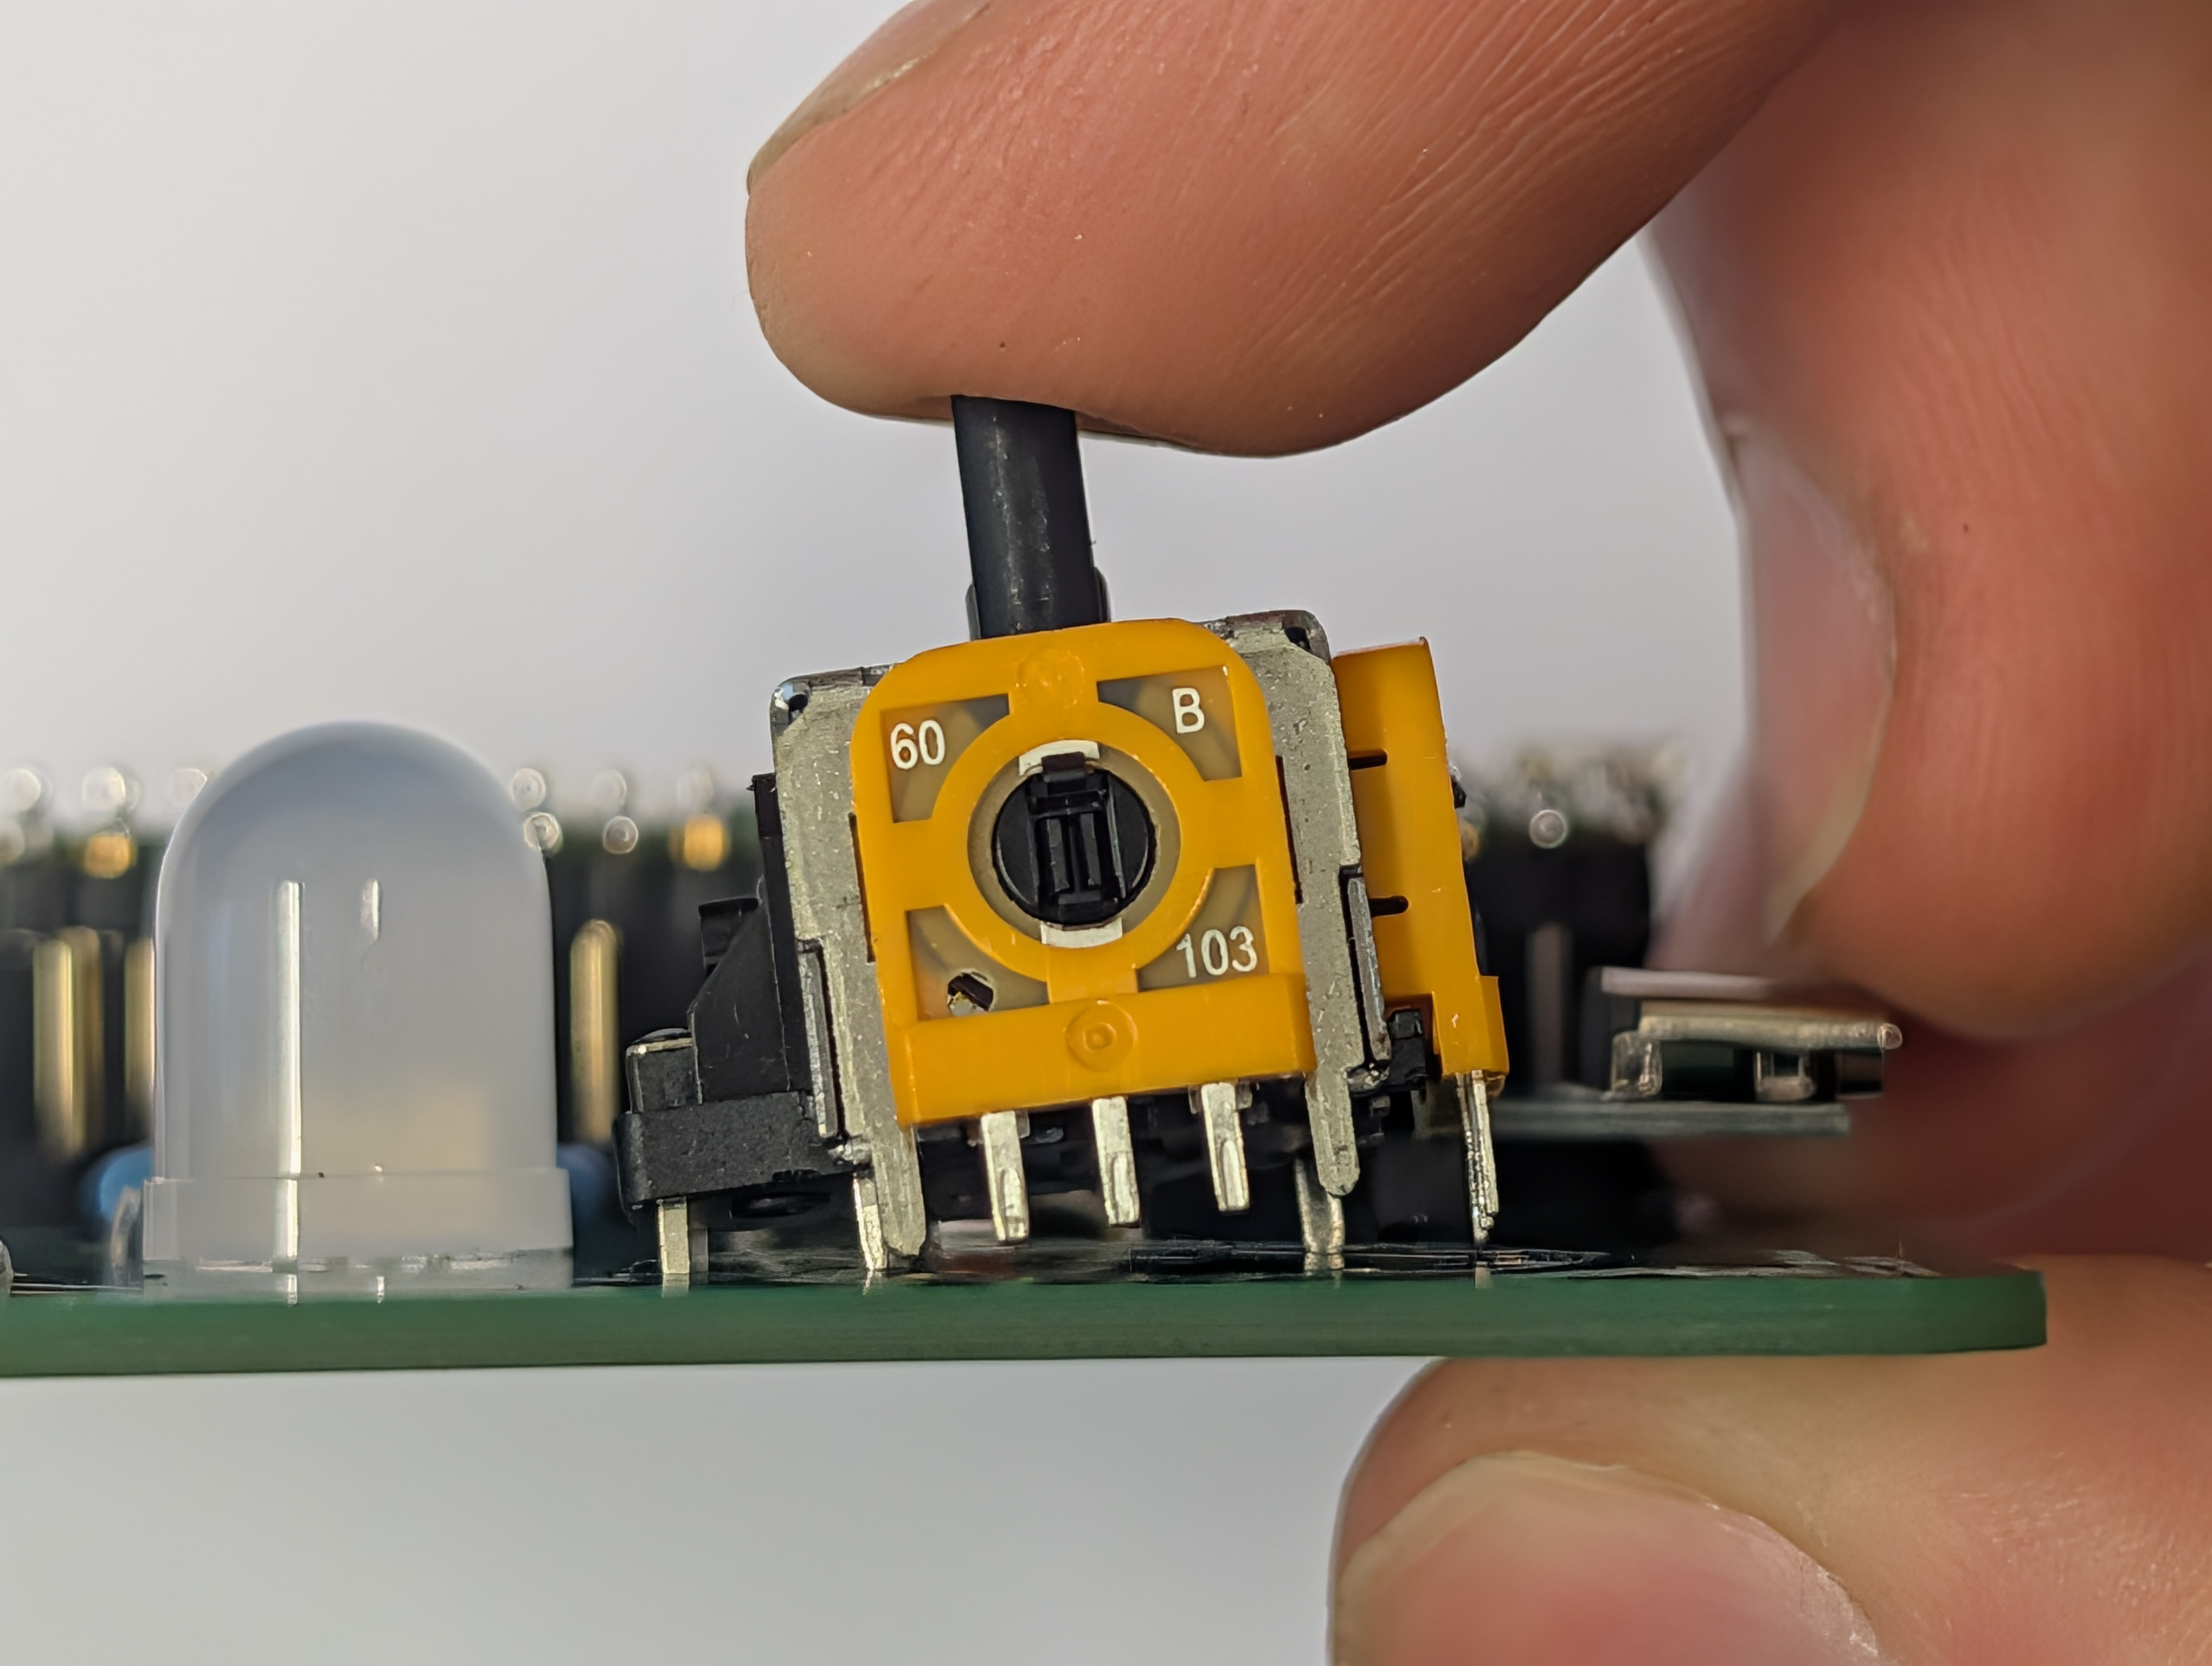
\includegraphics[width=0.75\textwidth]{pictures_of_construction/instruction_step_77.jpg}
\end{figure}

\begin{figure}[H]
    \centering
    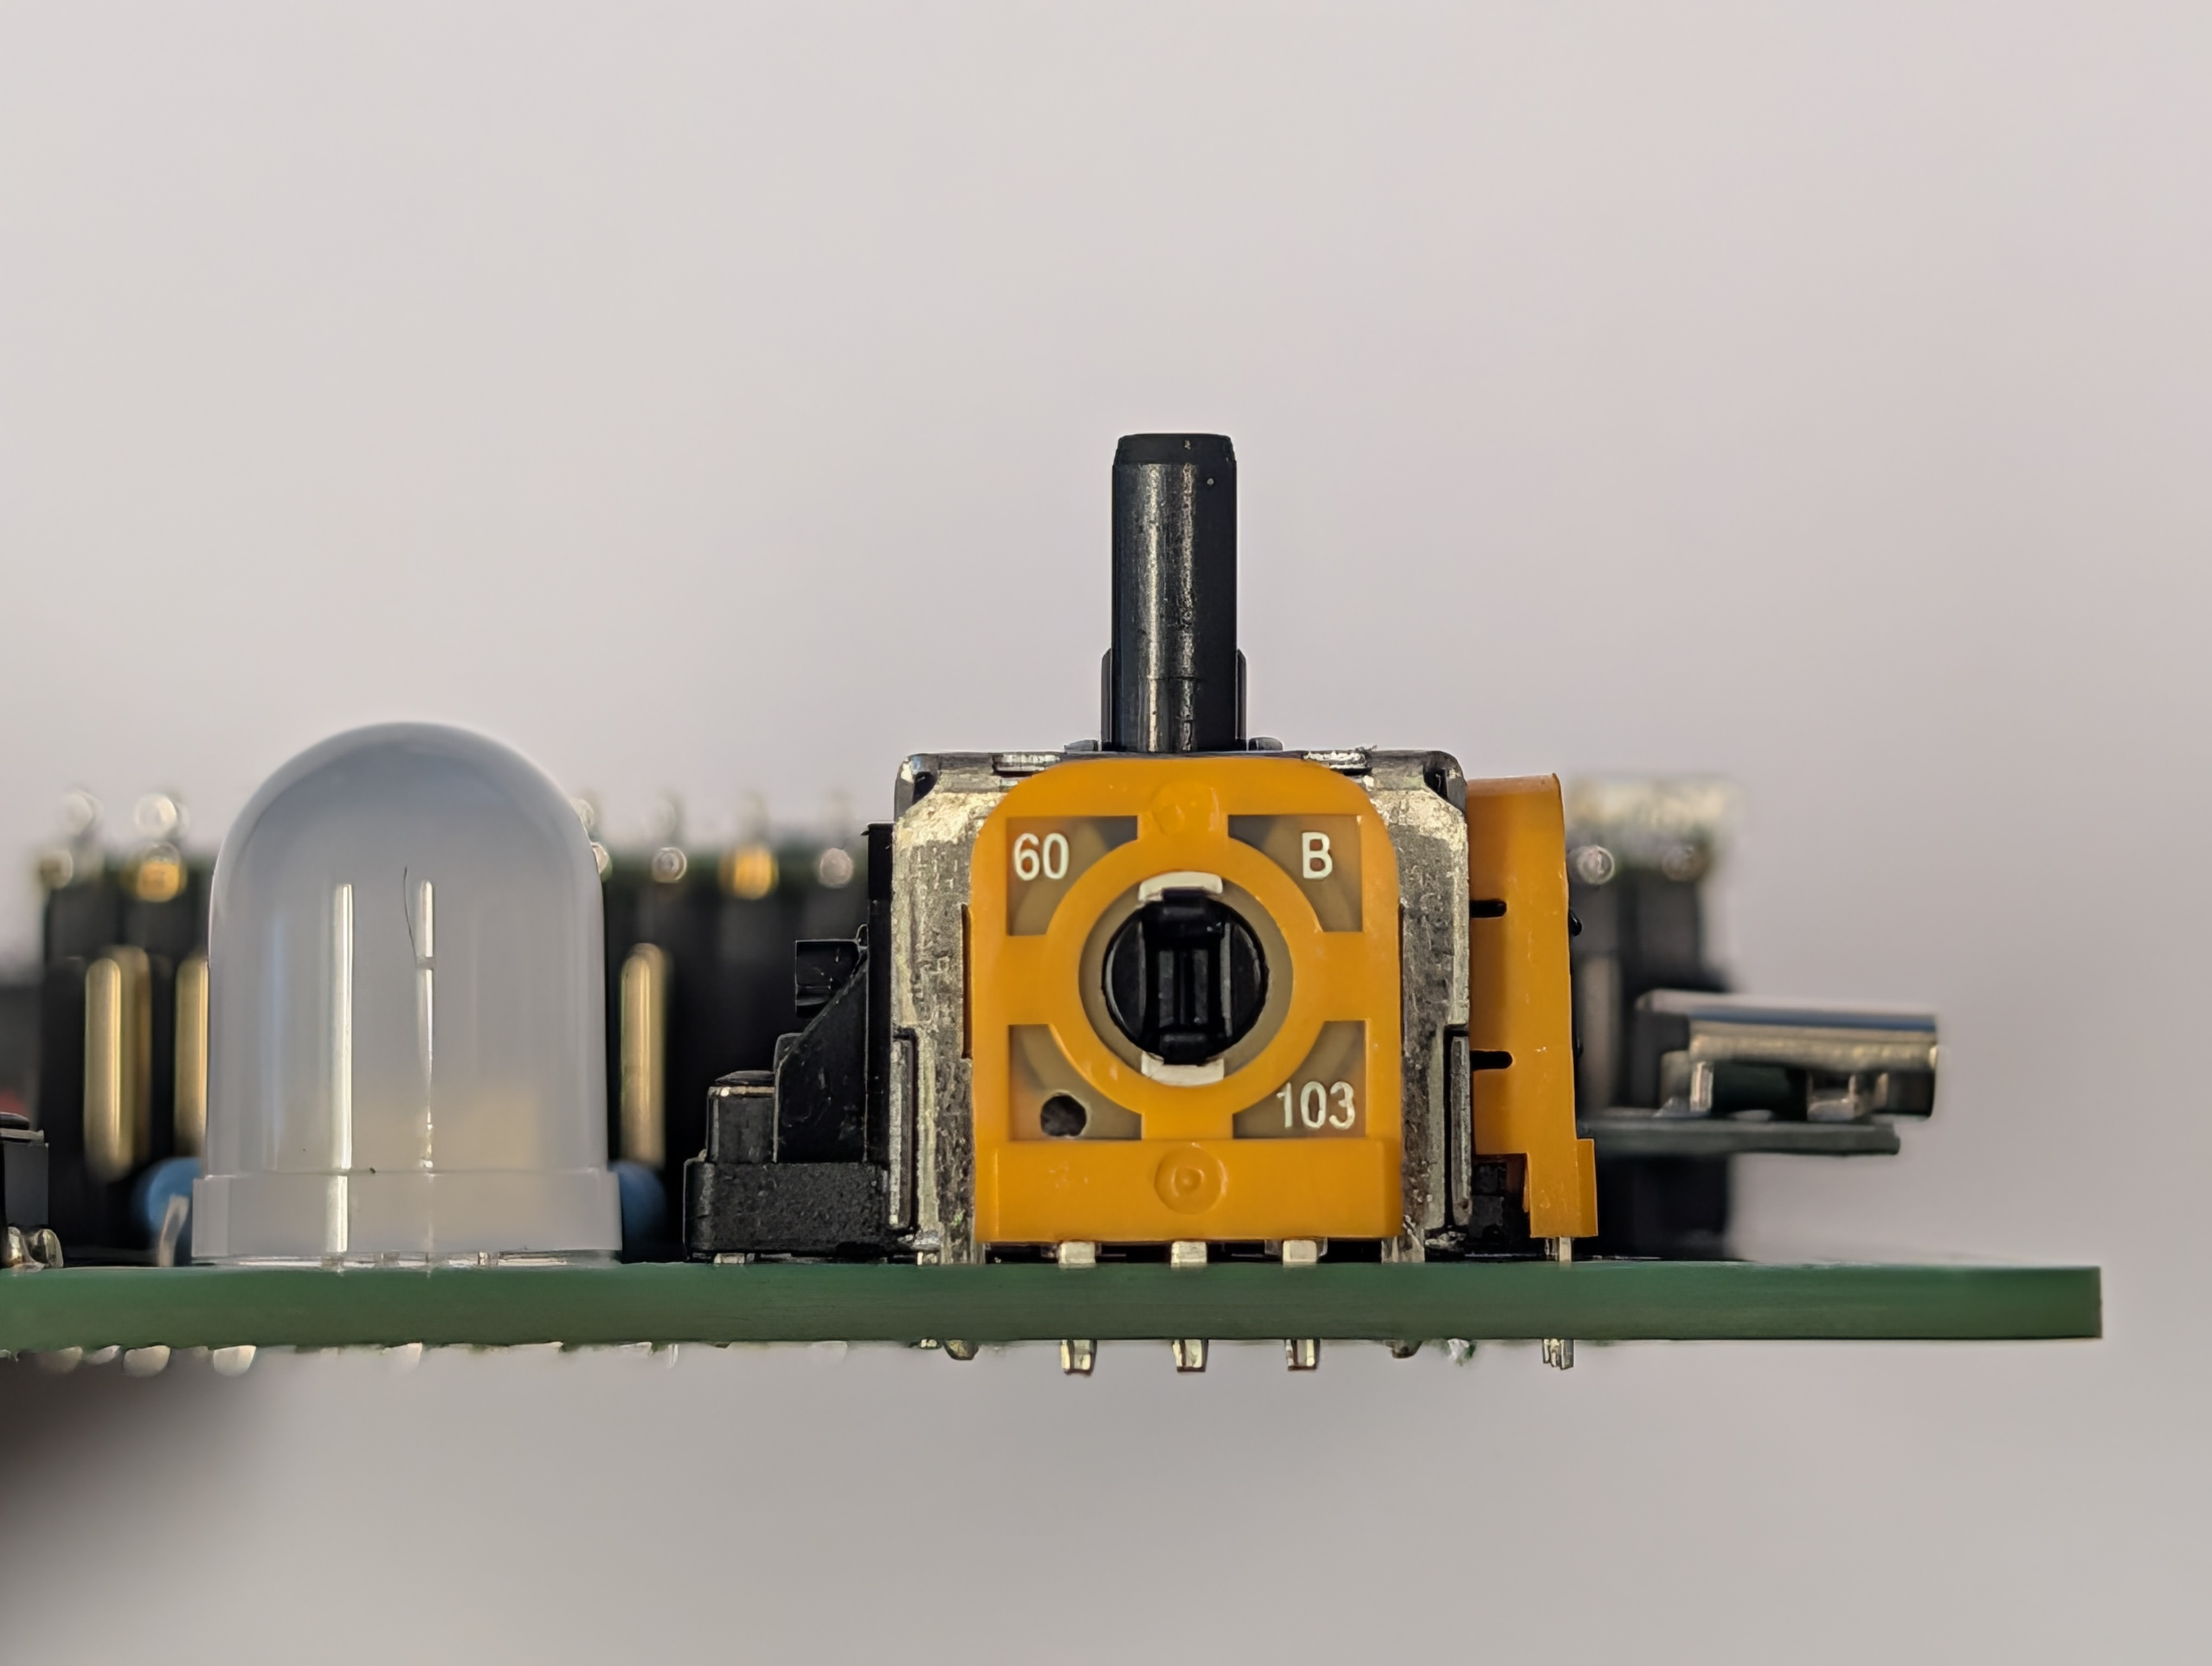
\includegraphics[width=0.75\textwidth]{pictures_of_construction/instruction_step_78.jpg}
\end{figure}

The installation of the joystick can be harder than necessary because of the many different pins. Start by putting the push-button pins into the Buzzerino PCB and then wiggle each pin from left to right slowly into position. After the joystick is fully seated, you can solder it in place.

\begin{figure}[H]
    \centering
    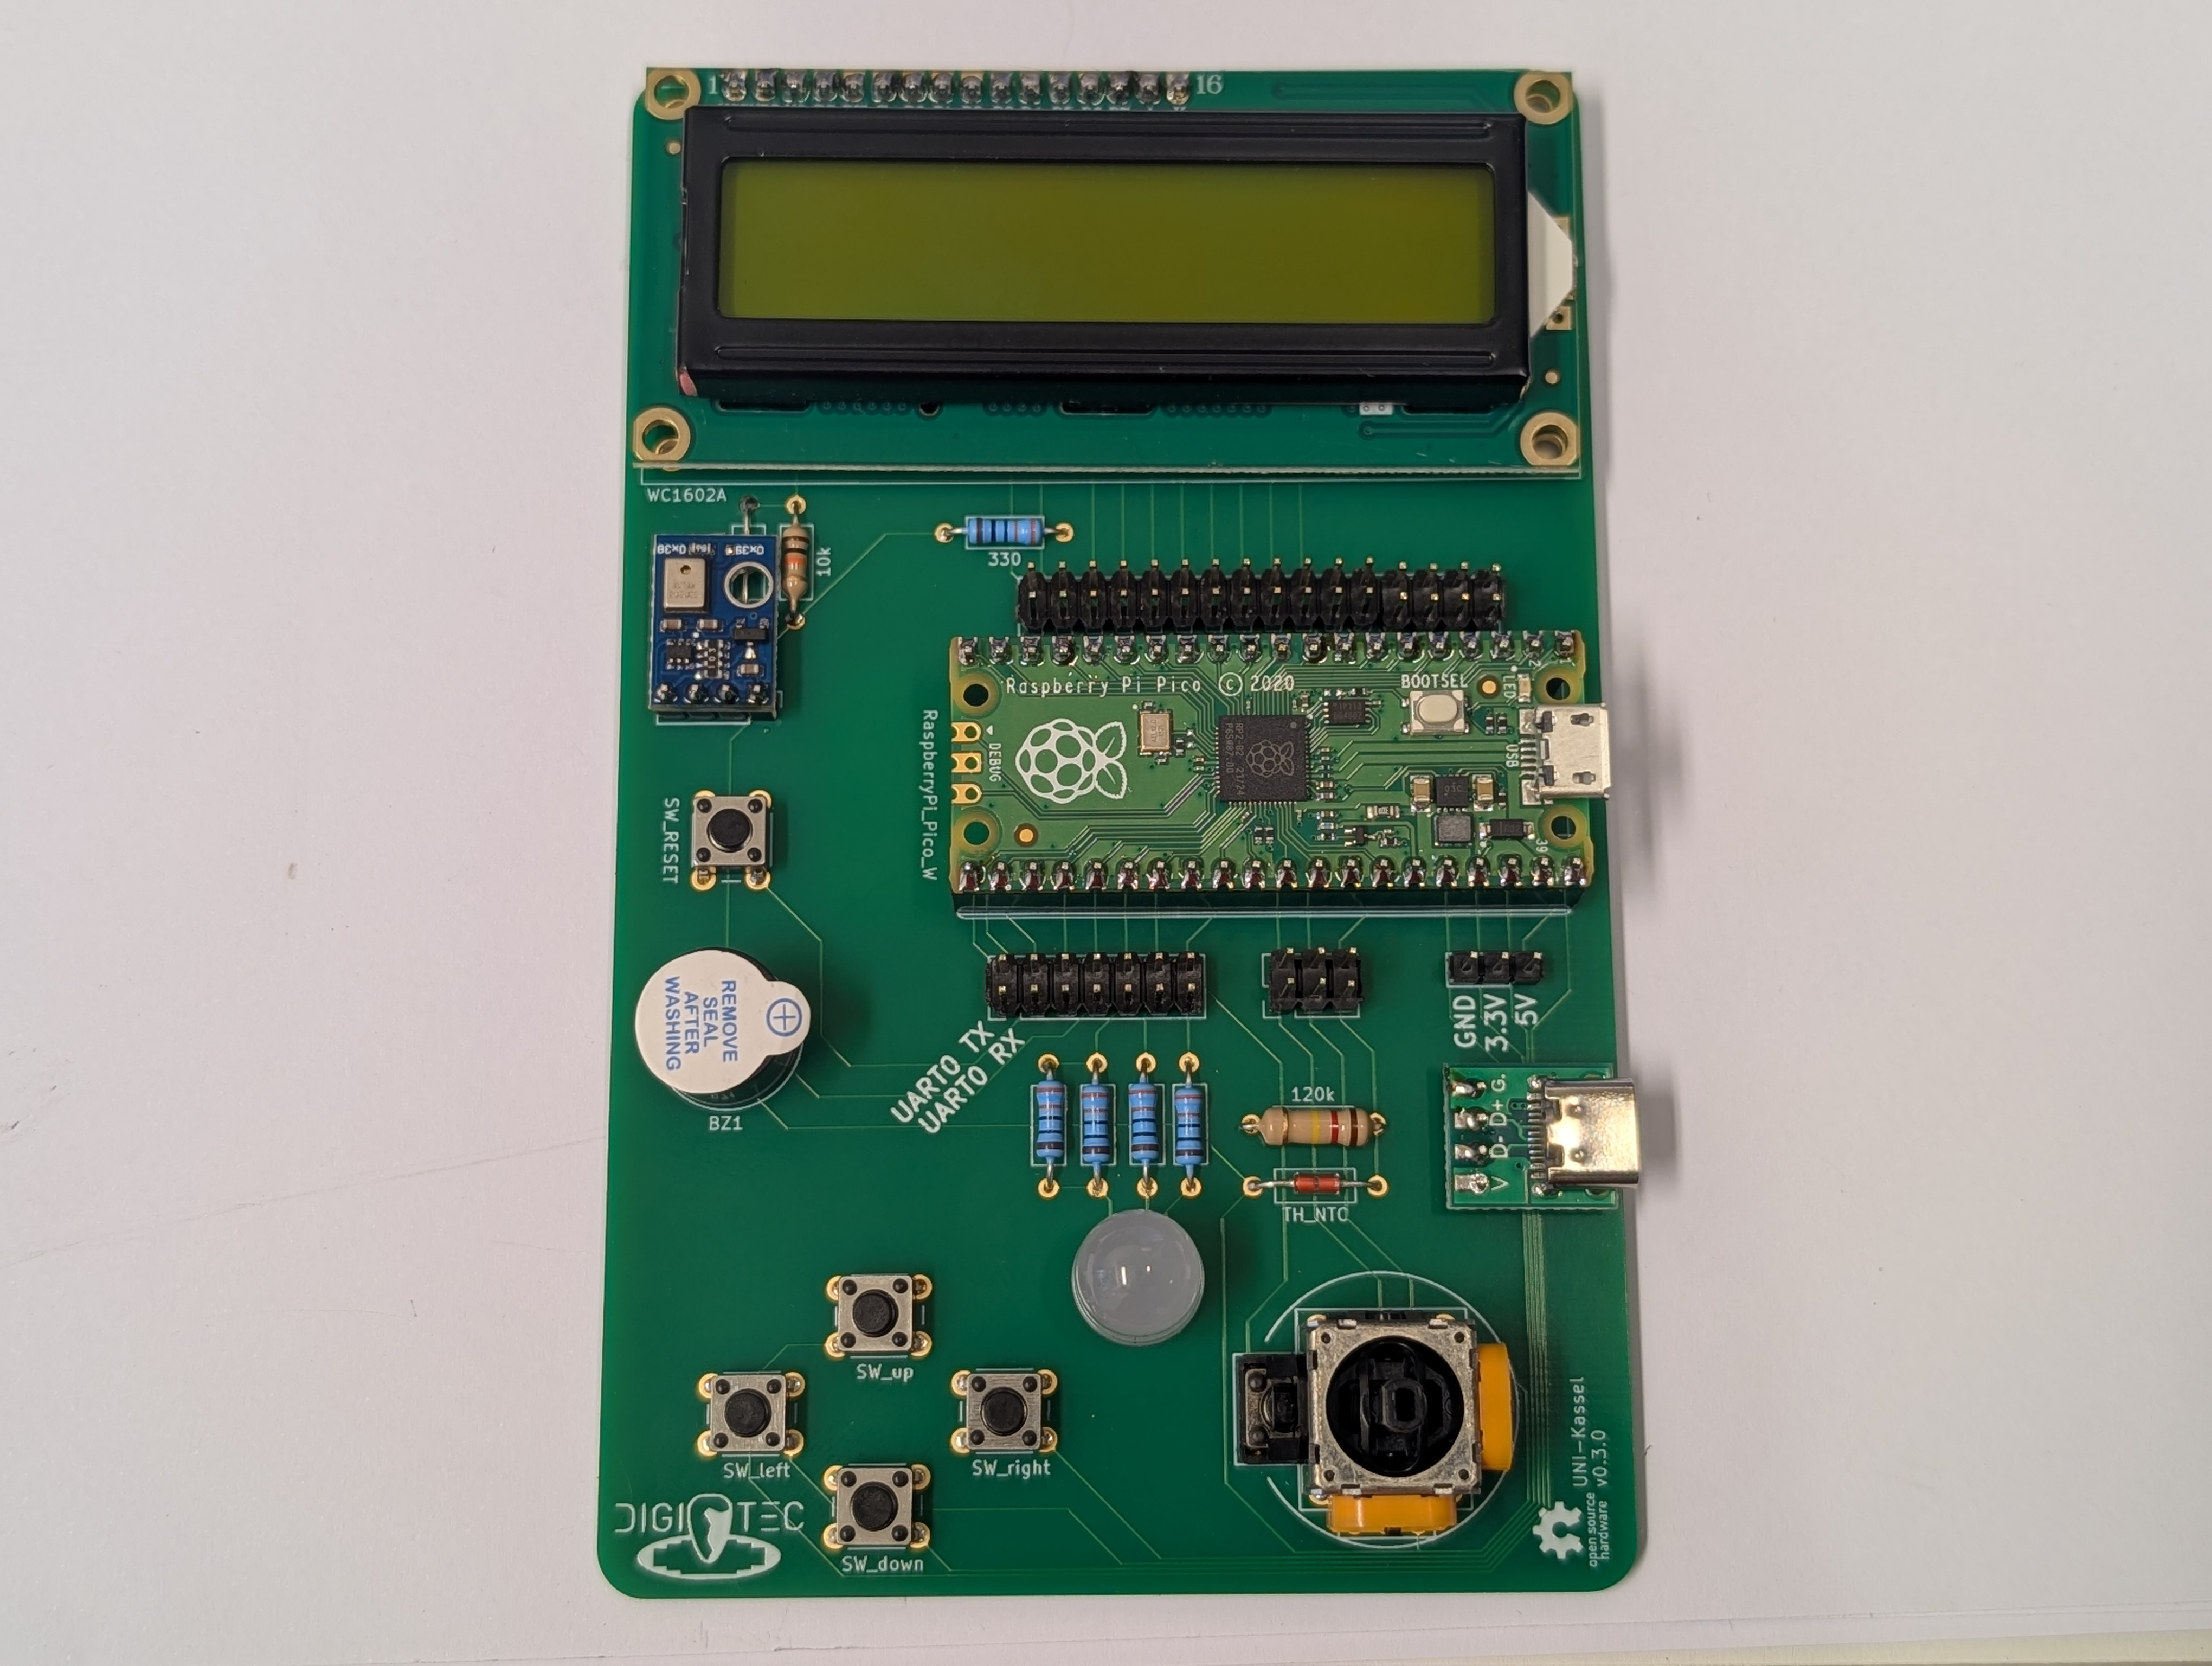
\includegraphics[width=0.75\textwidth]{pictures_of_construction/instruction_step_79.jpg}
\end{figure}

\subsection*{Installation of the jumpers}

\begin{figure}[H]
    \centering
    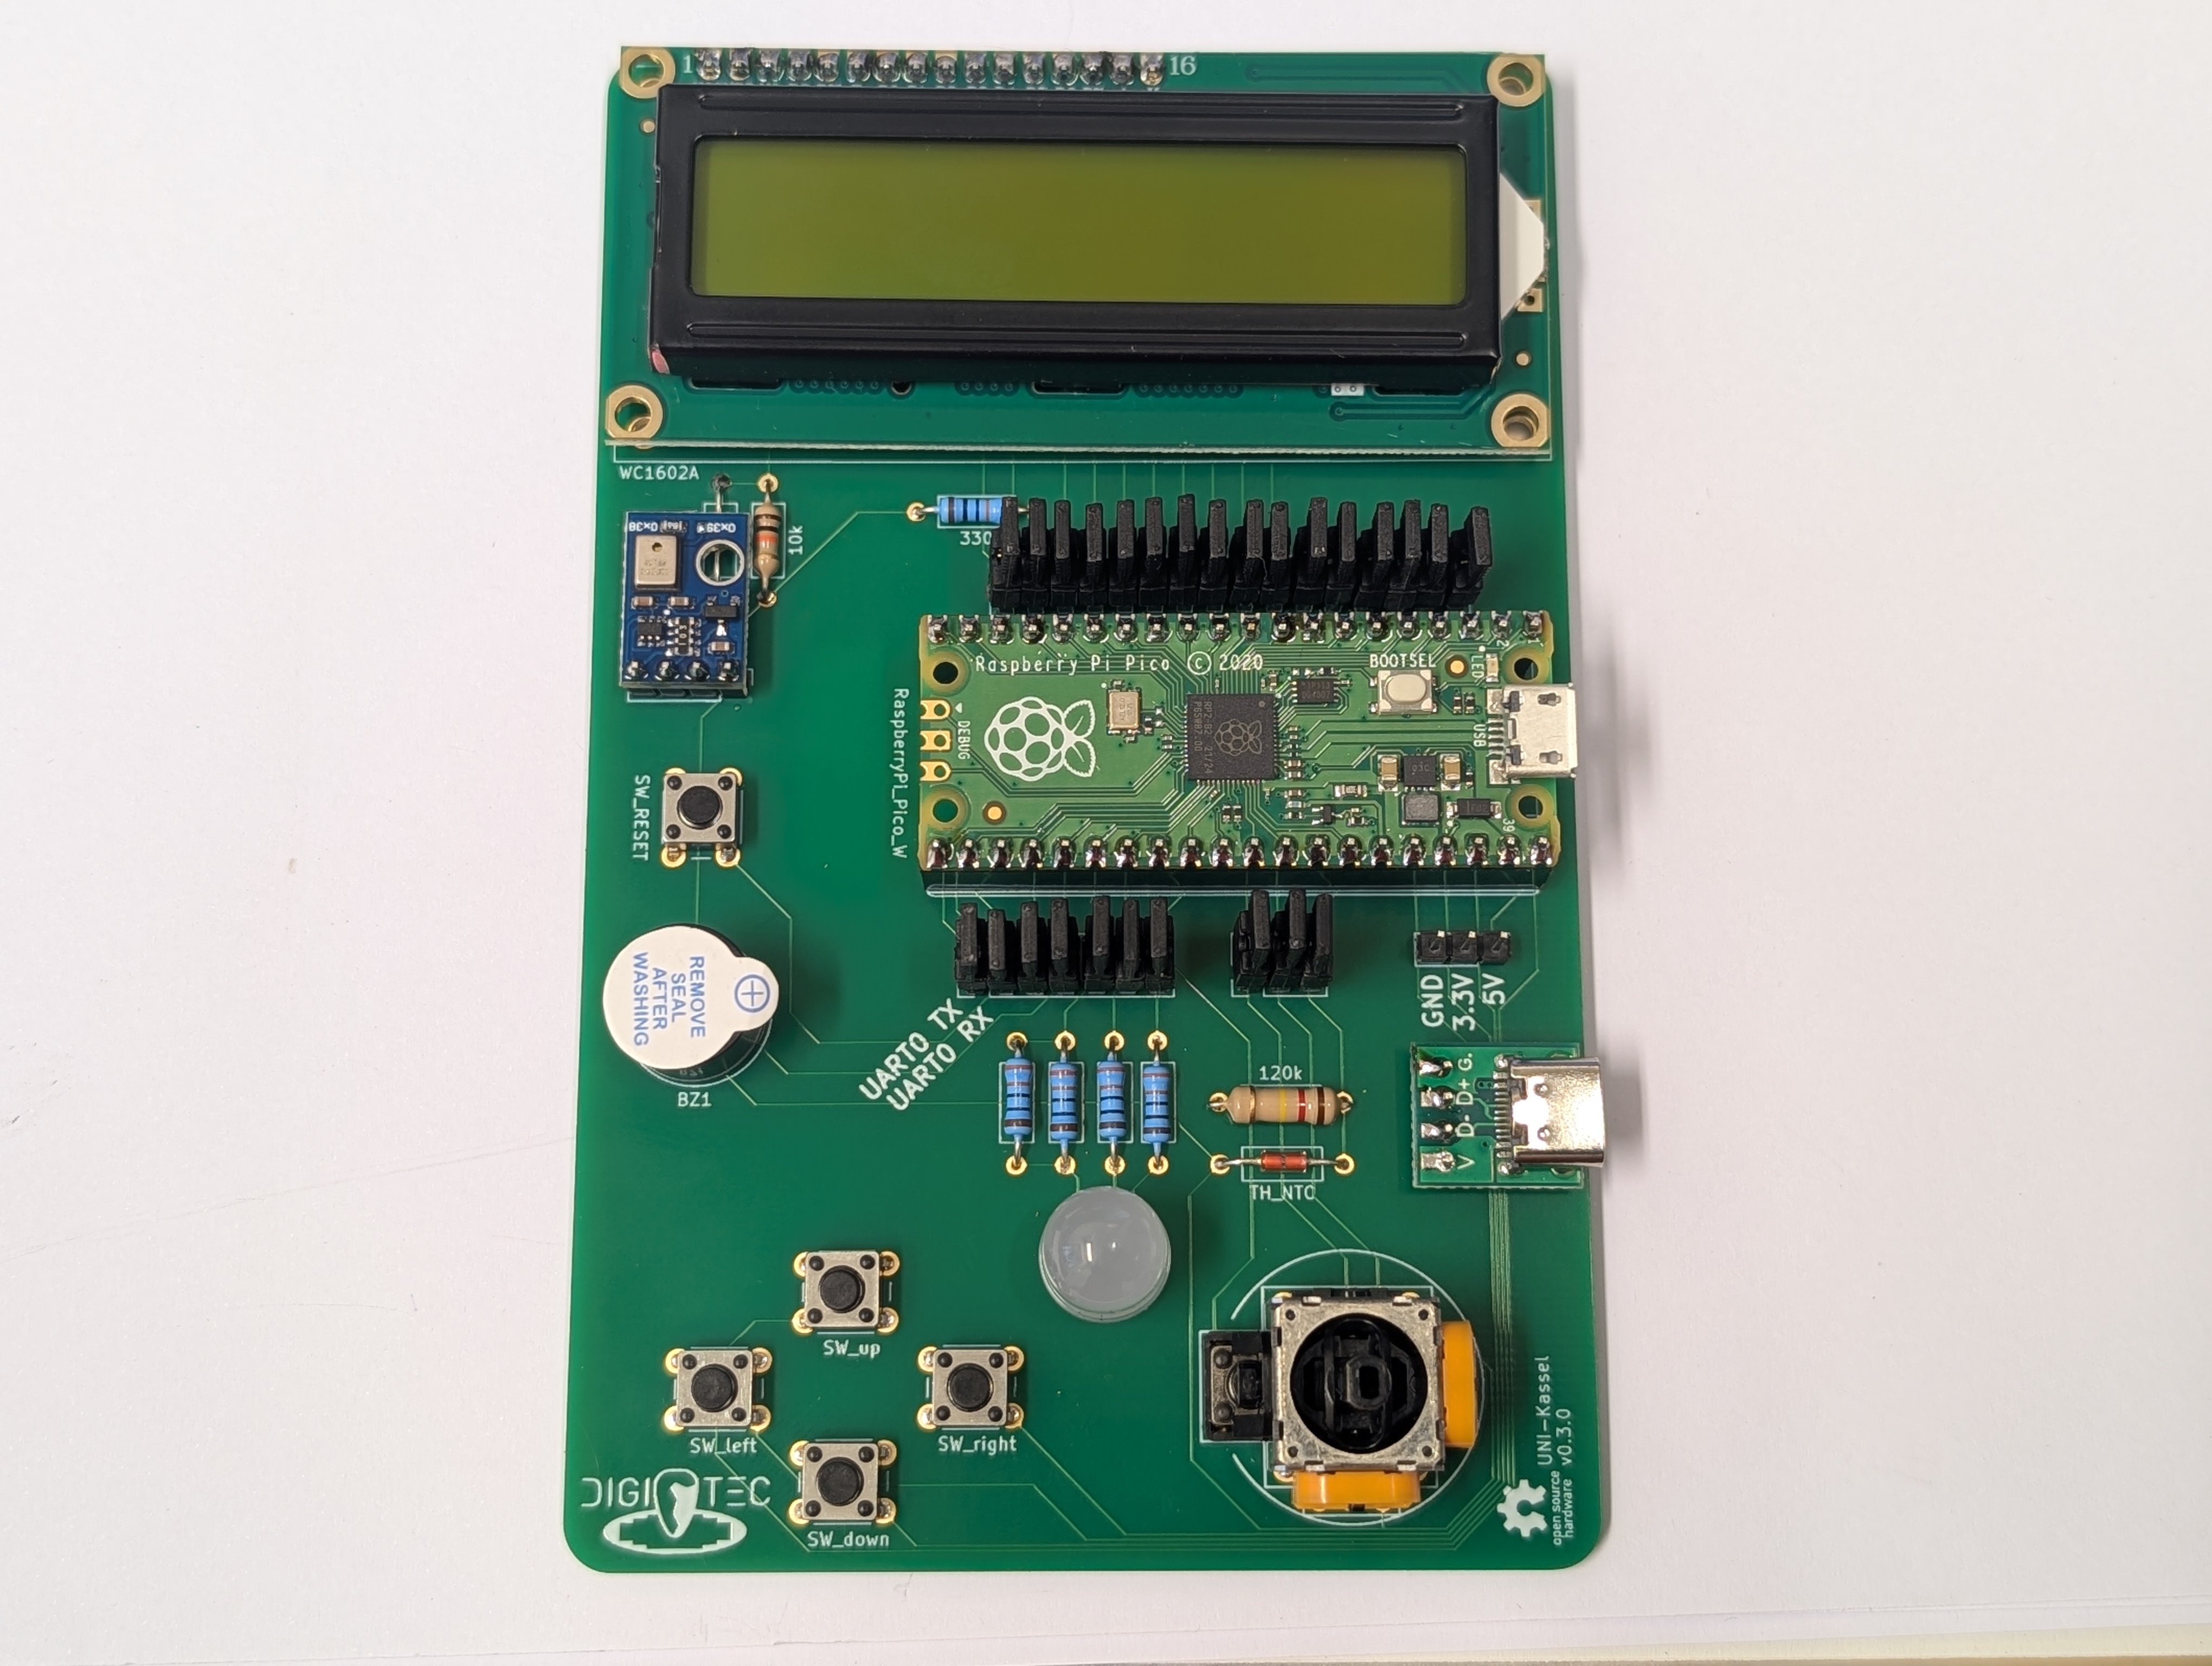
\includegraphics[width=0.75\textwidth]{pictures_of_construction/instruction_step_80.jpg}
\end{figure}

Before testing the board, we need to install all 26 jumpers as seen in the picture above.

\textbf{Congratulations, you have finished your soldering project.}

If you already flashed your Raspberry Pi Pico, it is time to power it up; if not, flash the \texttt{self\_test.uf2} onto the board.

\section*{Flashing}

If the board is not connected to a power source: press and hold the \textbf{BOOTSEL} button on the Raspberry Pi Pico and connect it via micro-USB to a PC. The Pico should mount as a mass-storage device called \textbf{RPI-RP2}. Now you can drag and drop a previously compiled or downloaded \texttt{.uf2} file onto it. It will automatically unmount and reboot. Ignore the message from your PC that the device was disconnected without ejecting.

You do not need to unplug and replug the Raspberry Pi Pico every time you want to flash it. You can also, with an established connection to your PC, press and hold the \textbf{BOOTSEL} button on the Raspberry Pi Pico and then briefly press (while still holding the \textbf{BOOTSEL} button) the \textbf{SW\_RESET} button on the Buzzerino PCB.

\section*{Example Programs}

The code of the example programs and their \texttt{.uf2} files are available in the folder \texttt{example\_programs}. Unless otherwise noted, all programs are designed and compiled for the Raspberry Pi Pico (neither the W version nor version 2) but can be recompiled for these targets. The preferred way to compile is VS Code with the Raspberry Pi Pico extension.


\end{document}